%\documentclass[b5paper,final,11pt,fleqn,twoside]{book}

\documentclass[a4paper,final,11pt,fleqn,twoside]{book}  %% ATENCIÓN: draft|final
%
% cabeceras.tex
%
% Copyright 2003, Diego Berrueta Muñoz
%
% Cabeceras comunes
%

\usepackage[T1]{fontenc}

%Glosario

\usepackage[toc,style=treenoname,order=word,counter=section]{glossaries}

\usepackage{xspace}


\usepackage{tikz,times}
\usetikzlibrary{mindmap,backgrounds}

% cambia algunas fuentes (utilidad dudosa)
\usepackage[scaled=0.92]{helvet}
\usepackage{pifont}
\usepackage{courier}

% cambia algunas fuentes en modo matemático a Palatino
\usepackage{mathpazo}

% españolización
\usepackage[spanish]{babel}
\usepackage[utf8]{inputenc}
%\extrasspanish

% gráficos y colores
\usepackage{rotating}
\usepackage{graphicx}
\usepackage{color}
%\usepackage[all]{xy}
%\usepackage{pstricks}
\usepackage{pst-node}
%\usepackage[dvips,usenames]{pstcol}
%\usepackage{pdftricks}
%\usepackage{pst-uml}  % para hacer diagramas UML
%\usepackage{rail}     % para hacer diagramas de gramáticas

% mejoras visuales
\usepackage{enumerate}
\usepackage{fancyhdr}  % para configurar los encabezados
\usepackage{fancybox}  % para hacer cajitas
\usepackage[normal,oneline,sf,bf]{caption2}
\usepackage{titlesec}  % para configurar los títulos de sección
\usepackage{paralist}


\usepackage{epigraph}

% citas, referencias e índices
\usepackage{cite}
%\usepackage{citesort}   % da errores al compilar
\usepackage{makeidx}

% incrustaciones de código fuente
%\usepackage[norules,nolineno]{lgrind}
\usepackage{verbatim}
\usepackage{listings}
%\usepackage{noweb,a4wide}


%\usepackage{textcomp}
\usepackage[right]{eurosym}

% columnas
\usepackage{multicol}

% tablas
\usepackage{longtable}
%\usepackage{ltxtable}

% impresión elegante de URLs
\usepackage{url}

\makeatletter
\def\url@pfcstyle{%
  \@ifundefined{selectfont}{\def\UrlFont{\sf}}{\def\UrlFont{\small\ttfamily}}}
\makeatother
%% Now actually use the newly defined style.
\urlstyle{pfc}


% márgenes
\usepackage[a4paper, left=30mm, right=20mm, top=25mm, bottom=25mm]{geometry}
%\usepackage[a4paper, left=20mm, right=20mm, top=25mm, bottom=25mm]{geometry}

% 
% \usepackage[a4,center,cam]{crop}
\usepackage{blindtext}

% salida en PDF navegable
%\usepackage{hyperref}
\usepackage[plainpages=false,colorlinks, linkcolor=black]{hyperref}

% quitar en versión final
%\usepackage{showkeys}   % depuración de etiquetas y referencias
%\usepackage{showidx}    % depuración de índice

% configuración del paquete "listings"

\lstset{%
        %language=Java,
	basicstyle=\footnotesize\sffamily,
	keywordstyle=\bfseries, %\color{darkred}
 	stringstyle=\itshape, %\color{violet}
 	commentstyle=\itshape, %\color{blue}
 	showspaces=false,
 	showtabs=false,
 	showstringspaces=false,
 	frame=trBL,
        frameround=tttt,
        %backgroundcolor=\color{lightyellow},
	inputencoding=utf8,
 	extendedchars=true,
 	numbers=none,
        aboveskip=0.5cm,
        belowskip=0.5cm,
        xleftmargin=1cm,
        xrightmargin=1cm,
	breaklines=true
}
\definecolor{darkred}{rgb}{0.5, 0, 0}
\definecolor{violet}{rgb}{1, 0, 1}
\definecolor{lightyellow}{rgb}{1,1,0.8}


%%%%%%%%%%%%%%%%%%%%%%%%%%%%%%%%%%%%%%%%%%%%%%%%%%%%%%%%%%%%%%%%%%%%%%
% cabeceras y pies de página (con el paquete "fancyhdr")
\headheight 15pt
%\addtolength{\headwidth}{\marginparsep}
%\addtolength{\headwidth}{\marginparwidth}
%\renewcommand{\chaptermark}[1]{\markboth{\MakeUppercase{#1}}{}}
%\renewcommand{\sectionmark}[1]{\markright{\thesection\ #1}}
%\fancyhead[LE,RO]{\textbf{\thepage}}
%\fancyhead[RE]{\textit{\leftmark}}
%\fancyhead[LO]{\rightmark}
%\fancyfoot[LCR]{}
\fancyhead{} % Todos los campos en blanco en la cabecera
\fancyfoot{} % Lo mismo al pie
\fancyhead[RO, LE]{\thepage}
\fancyhead[LO, RE]{\slshape\leftmark}
\renewcommand{\headrulewidth}{0.5pt}
\renewcommand{\footrulewidth}{0.5pt}


%%%%%%%%%%%%%%%%%%%%%%%%%%%%%%%%%%%%%%%%%%%%%%%%%%%%%%%%%%%%%%%%%%%%%%
% títulos de secciones (con el paquete "titlesec")
\titleformat{\chapter}[display]
	{\fontfamily{pag}\selectfont\Huge}
	{\LARGE\chaptertitlename\ \thechapter}{20pt}{\bfseries}
\titleformat{\section}
	{\fontfamily{phv}\selectfont\LARGE}
	{\thesection}{1em}{\bfseries}[\titlerule]
\titleformat{\subsection}
	{\fontfamily{phv}\selectfont\Large}
	{\thesubsection}{1em}{\bfseries}
\titleformat{\subsubsection}
	{\fontfamily{phv}\selectfont\large}
	{\thesubsubsection}{1em}{\bfseries}


%%%%%%%%%%%%%%%%%%%%%%%%%%%%%%%%%%%%%%%%%%%%%%%%%%%%%%%%%%%%%%%%%%%%%%
% espaciado entre párrafos
\addtolength{\parskip}{+0.2cm}


%%%%%%%%%%%%%%%%%%%%%%%%%%%%%%%%%%%%%%%%%%%%%%%%%%%%%%%%%%%%%%%%%%%%%%
% salida en PDF navegable (con el paquete "hyperref")
\hypersetup{bookmarks,
	bookmarksnumbered,
%	colorlinks, % quitar en las versiones impresas
	hyperindex,
	%linkcolor=red,
	%anchorcolor=black,
	%citecolor=green,
	citecolor=violet,
	%filecolor=magenta,
	%menucolor=red,
	%pagecolor=red,
	%urlcolor=cyan,
	pdftitle={PhD. Dissertation-Jose María Alvarez Rodríguez},
	pdfauthor={Jose María Alvarez Rodríguez}
	pdffitwindow,
	plainpages=false,
	pageanchor=false,
	pdfstartview={}}


%%%%%%%%%%%%%%%%%%%%%%%%%%%%%%%%%%%%%%%%%%%%%%%%%%%%%%%%%%%%%%%%%%%%%%
% profundidad de secciones y numeración
%\setcounter{tocdepth}{4}
\setcounter{secnumdepth}{3}


%%%%%%%%%%%%%%%%%%%%%%%%%%%%%%%%%%%%%%%%%%%%%%%%%%%%%%%%%%%%%%%%%%%%%%
% división silábica
\hyphenation{pu-bli-ca-ción con-tex-tua-li-za-ción pro-ble-mas Mi-nis-te-rio li-ci-ta-ción si-guien-tes desa-rro-llar con-tra-ta-ción pan-europea fa-ci-li-tar in-ter-opera-bility
 elec-tró-ni-ca li-ci-ta-do-ras he-te-ro-gé-neos res-trin-gi-do cons-cien-te de-sa-rro-lla-da mo-de-lo paí-ses ge-ne-ra-da
 par-ti-ci-pa-ción ad-mi-nis-tra-ti-vos bi-blio-gra-fía re-gis-tra-do-ra ad-mi-nis-tra-ti-va ca-rac-te-rís-ti-cas
 Pa-ra-le-la-men-te des-cri-ben vo-ca-bu-la-rio me-dian-te do-cu-men-to di-fe-ren-tes bi-blio-gra-fía mo-de-lo
 ve-ri-fi-ca rea-li-zar res-tric-ciones Por ejem-plo su-ge-ren-cias mo-de-los rea-li-za si-guien-do he-te-ro-gé-neas ello
 ra-zo-na-ble li-mi-ta-cio-nes reu-ti-li-cen ini-cia-ti-va va-ria-da exis-ten ob-te-ner con-ti-nua-men-te me-dian-te ins-ti-tu-ción
 pro-pues-ta pu-bli-ca-ción ca-tá-lo-go mo-ni-to-ri-za-ción vi-sua-li-za-ción mo-de-los co-rres-pon-dien-tes
 re-fe-ren-cia re-la-ti-vas par-ti-cu-lar  ele-men-to mo-de-la-do se-le-ccio-na-do pro-du-cción Re-con-ci-lia-ción des-crip-cio-nes broader-Transitive 
 de-pen-dien-do Ca-tá-lo-gos vo-ca-bu-la-rios Pro-pie-ta-rio des-plie-gue De-sa-rro-lla-dor mo-de-lar res-pues-ta si-mi-la-res rea-li-za-do SE-RI-MI 
Evol-ving ha-bi-li-tar rea-li-za-ción pu-bli-ca-ción ge-ne-ra-ción rea-li-za-ban ac-tua-li-za-ción ac-ce-so ha-cer es-tán-dar 
vo-ca-bu-la-ry con-si-de-ra-do des-cri-bir pu-bli-car pu-bli-ca-dos ta-xo-nó-mi-ca Pro-duct-on-to-lo-gy Va-lo-res in-terope-ra-bi-li-dad MOL-DEAS 
man-te-ni-mien-to re-pre-sen-tar ta-xo-no-mías des-crip-ción ge-ne-ra cons-truc-ción re-pre-sen-tan-do rea-li-za-das trans-fe-ren-cia 
uti-li-za-ble pu-bli-ca be-ne-fi-cios res-pon-sa-bi-li-da-des rea-li-zan Ad-mi-nis-tra-ción con-ti-nua-ción prio-ri-ta-rio ICT 
in-terope-ra-ble ge-ne-ra-do con-fi-gu-ra-cio-nes rea-li-zan-do rea-lis-ta má-xi-mo Cons-ti-tu-yen-do pro-ble-ma po-si-bi-li-dad ma-yor coo-pe-ra-ción 
ra-zo-na-mien-to Des-crip-tion con-cep-tua-li-za-ción de-sa-rro-lla-dos ope-ra-do-res axio-mas go-bier-no or-ga-nis-mos éxi-to 
si-guien-te do-mi-nios pro-duc-ción Na-tio-nal orien-ta-da ló-gi-ca in-di-vi-duos di-se-ña-do for-ma-li-za-dos ta-xo-no-mía 
auto-má-ti-ca ca-li-dad re-co-men-da-ble ad-mi-nis-tra-ti-vo su-mi-nis-tre error ca-rac-te-rís-ti-ca ele-men-tos he-rra-mien-tas 
eva-lua-ción res-pec-to Ad-mi-nis-tra-cio-nes ex-pe-ri-men-tal orien-ta-das re-gis-tros do-cu-men-tos má-xi-ma je-rar-quía 
sa-tis-fac-to-rios obs-tan-te con-su-mi-dos con-fe-ren-cias SPARQL rea-li-za-dos va-lo-ran eco-no-mi-zar fle-xi-ble ex-pe-dien-te 
pro-ce-di-mien-to usan-do ame-ri-ca-nas fa-mi-lia ni-vel ra-zo-na-do-res re-pre-sen-ta-ción lo-ca-li-za-do Man-ches-ter 
en-ri-que-ci-mien-to he-rra-mien-ta rea-li-zar-se prio-ri-ta-rios Li-ci-ta-cio-nes ne-ce-sa-rios ma-te-ria-li-zan es-pe-cia-li-zán-do-se 
Com-pu-ting pla-ni-fi-ca-ción cua-li-ta-ti-va de-sa-for-tu-na-da-men-te li-de-ra-do ma-te-ria-li-za-do Cons-tructs 
ma-te-ria-li-za WESO en-ten-di-mien-to MOLDEAS ela-bo-ra-ción re-fe-ren-te re-gis-tra-tion uni-la-te-ral po-si-bi-li-tar ope-rar 
in-ter-ope-ra-bles ad-mi-nis-tra-ti-vas fle-xi-bi-li-dad auto-no-mía co-mer-cio procesa-miento de-sa-rro-llan-do meta-in-for-ma-ción 
apro-pia-dos li-mi-ta-do es-pe-cia-li-za-ción ló-gi-cas in-de-pen-dien-te-men-te ge-ne-ral dis-po-ner dis-mi-nu-yen-do co-rrien-te 
rea-pro-ve-char de-sa-rro-llo ge-ne-ral Ins-ti-tu-te com-pu-ting pos-te-rior con-su-mi-da mi-llo-nes Fi-gu-ras cons-tan-te equi-va-len-cia ope-ra-cio-nes 
fac-to-ri-za-ción Res-pon-sa-bles Geo-Linked-Data reu-ti-li-za-ción co-rrec-tos trans-for-ma-ción bien con-si-guien-te des-cu-brien-do 
geo-rre-fe-ren-cia-ción pro-li-fe-ra-ción cum-pli-mien-to Ne-go-tia-ted uti-li-dad ma-nual es-pe-cia-li-za-ción ma-yo-ría mo-de-la 
des-cu-bri-mien-to rea-li-za-da pu-bli-can se-lec-cio-nar me-ca-nis-mos fun-cio-na-li-dad ve-ri-fi-car ines-pe-ra-dos re-gis-tro 
pro-pues-tos trans-pa-ren-te va-ria-bles bi-blio-te-ca bi-blio-te-cas adap-ta-bi-li-dad in-ter-co-ne-xión va-ria-ble vi-sua-li-zar 
ope-ra-ti-vo ge-ne-rar su-mi-nis-tra-dos va-li-da-ción su-mi-nis-tra-dores pro-pie-da-des hi-po-ni-mia re-cu-pe-ra-dos in-de-pen-dien-te-ment-te 
triun-fo reu-ti-li-za-ción ge-ne-ral apro-xi-ma-ción va-ria-bi-li-dad teó-ri-cas con-ti-nuo di-se-ño des-afor-tu-na-da-men-te In-dus-trial prin-ci-pios 
di-fe-ren-cia-das eva-lua-dos re-qui-si-tos co-la-bo-ra-cio-nes co-la-bo-ra-ción in-dus-tria-les Se-venth pon-de-ra-do re-po-si-to-rios 
ex-pe-ri-men-ta-les pu-bli-ci-tar co-la-bo-ra-ción bi-llo-nes Doc-to-ra-do re-so-lu-ción cul-tu-ra-les trans-cur-so Pa-rro-quias Lo-gics co-rrec-to 
sig-ni-fi-ca-do Aña-dien-do ope-ra-ción ma-ne-ra agi-li-zar con-fian-za per-so-na-les in-al-te-ra-dos re-la-ti-vos des-cri-bien-do 
se-ña-la-das vo-ca-bu-la-ries con-tex-tua-li-za-da Ba-rras cir-cuns-cri-bién-do-se for-ma-li-za-ción fa-ci-li-tan-do re-ali-men-ta-ción 
re-fe-ren-cias ma-ni-fes-tar-se CKAN lo-ca-li-dad dia-gra-ma ver-da-de-ra-men-te es-ta-ble-ci-mien-to con-si-de-ra ta-reas co-rrec-ta 
co-he-ren-te pos-te-rior-men-te apro-pia-das exac-tos va-rios pro-pues-to ex-pe-ri-men-to re-fe-ren-tes orien-ta-dos ha-bi-tual con-cre-tas 
con-fi-gu-ran afi-lia-ción Gi-ner va-lo-ra-ción res-pon-sa-bi-li-dad}   

%%Tablas
\addto\captionsspanish{
        \def\listtablename{\'Indice de tablas}%
        \def\tablename{Tabla}} 

%%%Math
\usepackage{latexsym}
\usepackage{amsmath}
\usepackage{amssymb}
\usepackage{amsthm}

\usepackage{algorithm}
\usepackage{algorithmic}
\usepackage{multirow}
\usepackage{rotating}


\newtheorem{theorem}{Theorem}[section]
\newtheorem{proposition}[theorem]{Proposición}
\newtheorem{lemma}[theorem]{Lema}
\newtheorem{definition}[theorem]{Definición}
\newtheorem{examples}[theorem]{Ejemplos}
\newtheorem{remarks}[theorem]{Remarks}
\newtheorem{corollary}[theorem]{Corolario}
\newtheorem{remark}[theorem]{Remark}
\newtheorem{example}[theorem]{Ejemplo}
\newtheorem{conjecture}[theorem]{Conjecture}
\newtheorem{note}[theorem]{Nota}



\newsavebox\FrameBox
\newenvironment{Frame}{%
  \par\setbox\FrameBox\hbox\bgroup\minipage{0.9\textwidth}\parskip\baselineskip\ignorespaces
}{%
  \endminipage\egroup\fbox{\box\FrameBox}\par
}

\newcommand{\si}{$\oplus$\xspace}
\newcommand{\no}{$\ominus$\xspace}
\newcommand{\na}{$\odot$\xspace}


%Extraer
\newcommand{\linkeddata}{\textit{Linked Data}\xspace}
\newcommand{\opendata}{\textit{Open Data}\xspace}
\newcommand{\lod}{\textit{Linking Open Data}\xspace}
\newcommand{\ogd}{\textit{Open Government Data}\xspace}
\newcommand{\datasets}{\textit{datasets}\xspace}
\newcommand{\dataset}{\textit{dataset}\xspace}
\newcommand{\provenance}{\textit{provenance}\xspace}
\newcommand{\trust}{\textit{trust}\xspace}
\newcommand{\egov}{\textit{e-government}\xspace}
\newcommand{\pusi}{\textit{Public Sector Information}\xspace}
\newcommand{\gd}{\textit{Government Data}\xspace}
\newcommand{\wod}{Web de Datos\xspace}
\newcommand{\wode}{\textit{Web of Data}\xspace}
\newcommand{\eproc}{\textit{\gls{e-Procurement}}\xspace}
\newcommand{\gld}{\textit{Government Linked Data}\xspace}


%
% utilidades.tex
%
% Copyright 2003, Diego Berrueta Muñoz
%
% Algunos comandos y entornos utilizados
%


%%%%%%%%%%%%%%%%%%%%%%%%%%%%%%%%%%%%%%%%%%%%%%%%%%%%%%%%%%%%%%%%%%%%%%
% Para llamadas de atención al margen

\reversemarginpar

\newcommand{\attention}{%
  \mbox{}\marginpar{\raggedleft \large\bfseries ! $\rightarrow$}%
}

\newcommand{\InlineFIXME}[1]{%
  {\bfseries\color{red} FIXME: #1}%
}

\newcommand{\FIXME}[1]{%
  \attention{}{\color{red}\bfseries #1}%
}


%%%%%%%%%%%%%%%%%%%%%%%%%%%%%%%%%%%%%%%%%%%%%%%%%%%%%%%%%%%%%%%%%%%%%%
% Comandos específicos de este proyecto

\newcommand{\FechaEntregaPFC}{2011}
\newcommand{\TituloPFC}{MÉTODOS SEMÁNTICOS DE REUTILIZACIÓN DE DATOS ABIERTOS ENLAZADOS EN LAS LICITACIONES PÚBLICAS}
\newcommand{\NumeroPFC}{}
\newcommand{\AreaPFC}{LENGUAJES Y SISTEMAS INFORMÁTICOS}
\newcommand{\AutorPFC}{Jose María Álvarez Rodríguez}
\newcommand{\TutorPFC}{José Emilio Labra Gayo}


\newcommand{\toriginal}[1]{\textit{#1}}

\newcommand{\simbolo}[1]{ %
  \textbf{\texttt{#1}} %
}




%
% portada.tex
%
% Copyright (c) 2003 Javier Noval
% Copyright (c) 2004 Diego Berrueta
%
% Macros para hacer la portada del proyecto. Adaptados por Diego
% Berrueta a partir de los cedidos por Javier Noval
%

\makeatletter

\newcommand{\PrintNumeroDocumentoPFC}[1]{DOCUMENTO N$^\mathrm{o}$ #1}
\newcommand{\SpaceAfterNombreDocumentoPFC}{\vspace{2cm}}

\newcommand{\pfctitlepage}[8]{% Parámetros: área, nº, título, proyectante, fecha, tutor, nº doc, título doc
	\cleardoublepage

	{\bfseries
		\begin{center}
                        % Escudo de la universidad
			{\LARGE UNIVERSIDAD DE OVIEDO}
			
			\vspace{0.75cm}
	    
			
\includegraphics[width=6cm]{../logo_uniovi}

			\vspace{1.25cm}
		      % Identificación de la escuela, el área
			{\LARGE SISTEMAS Y SERVICIOS INFORMÁTICOS PARA INTERNET}

			\vspace{1.25cm}
	      
			%{\Large ÁREA DE \uppercase{#1}}

			% Número del proyecto y título
% 			{\Large TRABAJO DE INVESTIGACIÓN N$^\mathrm{o}$ #2}
			{\Large TESIS DOCTORAL}

			\vspace{1cm}

			{\Large \uppercase{#3}}

			\vspace{1cm}

			{\Large Presentada por \\}
			\vspace{0.5cm}
		        {\Large Jose María Álvarez Rodríguez\\}
			\vspace{0.5cm}
			{\Large para obtención del título de Doctor por la Universidad de Oviedo\\}
			\vspace{1cm}
			%{\Large Oviedo 2012}
			{\Large Dirigida por el\\}
			\vspace{0.5cm}
		        {\Large Profesor Doctor D. José Emilio Labra Gayo\\}
			\vspace{1cm}
			{\Large Oviedo, Junio de 2012}

		\end{center}

		    \vspace{1cm}

                % Bloque inferior, con el escudo de la escuela, los
                % nombres del autor y el tutor, y la fecha
% 		{\Large \begin{tabular}{@{}l@{}p{10cm}@{}}
% 			\begin{minipage}{5cm}
% 				
\includegraphics[width=3.5cm]{../escudo2}	
% 			\end{minipage} &
% 			\begin{tabular}{@{}p{10cm}@{}}
% 				\uppercase{#4\\
% 				#5\\
% 				#6}
% 			\end{tabular}
% 		\end{tabular}}

% 		\vspace{0.5cm}
% 	{ \begin{tabular}{@{}l@{}p{10cm}@{}}
% 			\begin{minipage}{5cm}
% 			
% 	\begin{tabular}{|@{}p{5cm}@{}|}
% 				\hline  \\
% 				 \\
% 				\\
% 				\\
% 				\\
% 				 \hspace{2.5cm}\small{Vbº del Tutor} \\
% \hline
% 			\end{tabular}
% 		
% 			\end{minipage} &
% 		
% 		\end{tabular}}


	}

	\cleardoublepage
}

\newcommand{\pfctitle}[8]{% Parámetros: área, nº, título, proyectante, fecha, tutor, nº doc, título doc
        \pagestyle{empty}
	\pfctitlepage{#1}{#2}{#3}{#4}{#5}{TUTOR: #6}{#7}{#8}
       % \FDLNotice{}
        \setcounter{page}{1}
        \pagestyle{fancy}
}

\makeatother

\newcommand{\PortadaDocumentoPFC}[2]{% Parámetros: nº doc y título de documento
   \pfctitle{\AreaPFC}{\NumeroPFC}{\TituloPFC}{\AutorPFC}{\FechaEntregaPFC}{\TutorPFC}{#1}{#2}
}




%
% bibliografia-utils.tex
%
%
% Para insertar la bibliografía
%

\providecommand*{\phantomsection}{} % Para evitar errores si no usamos el hyperref

\newcommand{\insertbibliography}{%
  \cleardoublepage
  \phantomsection
  \renewcommand{\bibname}{Referencias}
  \addcontentsline{toc}{chapter}{\bibname}
  %\bibliographystyle{plain}
  %\bibliographystyle{unsrt}
  %\bibliographystyle{../bibliografia/these}
  \bibliographystyle{../bibliografia/pfc}

  % Bases de datos de bibliografía
  \bibliography{../bibliografia/moldeas,../bibliografia/metodos,../bibliografia/phd-references,../bibliografia/web,../bibliografia/intro,../bibliografia/linked-data,../bibliografia/experimentacion,../bibliografia/e-procurement,../bibliografia/semantic,../bibliografia/extra}  
}




\makeindex

\makeglossaries
\loadglsentries{glosario}


%%%%%%%%%%%%%%%%%%%%%%%%%%%%%%%%%%%%%%%%%%%%%%%%%%%%%%%%%%%%%%%%%%%%%%
\begin{document}

\title{\NombrePFC}
\author{\AutorPFC}
\date{\FechaEntregaPFC}
%\maketitle

%%%%%%%%%%%%%%%%%%%%%%%%%%%%%%%%%%%%%%%%%%%%%%%%%%%%%%%%%%%%%%%%%%%%%%
\frontmatter

\PortadaDocumentoPFC{1}{}

%\chapter*{To-Do List}
\begin{enumerate}
 \item Introducir valores de ONTOSPREAD en la tabla
 \item Transversales: ortografía, expresión escrita, hyphenation, Maquetación (segunda ronda)
% \item Contrastes de hipotésis, Wilcoxon no aporta demasiado
\end{enumerate}


%
% resumen.tex
%

\chapter*{Resumen}
Las Administraciones Públicas son uno de los mayores compradores de la Unión Europea, ya que
sus adquisiciones en conjunto representan un $17$\% del Producto Interior Bruto. La tendencia está encaminada 
a la agilización de este gran mercado de oportunidades para facilitar el acceso a las empresas, especialmente a 
las pequeñas y medianas empresas (PYMEs), posibilitando el acceso a la información presente 
en los contratos públicos, permitiendo así la construcción de un entorno de mercado competitivo. 

Desde otro punto de vista, el creciente uso de Internet durante los últimos años ha puesto de manifiesto un
nuevo entorno de ejecución para las aplicaciones, utilizando como nueva plataforma la Web. Nuevas tecnologías y paradigmas
están emergiendo para dar soporte al desarrollo y despliegue de aplicaciones y servicios, así como para la publicación de datos e información. 
En este sentido, iniciativas como la Web Semántica, en concreto el esfuerzo de \linkeddata dentro de la nueva ``Web de Datos'',
 intentan elevar el significado de los elementos y recursos que están disponibles en la web con el objetivo de mejorar 
la integración e interoperabilidad entre aplicaciones y facilitar el acceso a la información y los datos a 
través de modelos y formatos de datos de conocimiento compartido unificados.

En el caso particular del proceso de contratación pública electrónica surge la necesidad de abordar problemas de 
gran calado tales como la dispersión de la información, la heterogeneidad de los formatos de los anuncios, 
la diversidad de formatos de explotación o el multiling\"{u}ismo y multiculturalidad. Con el propósito de proporcionar 
una solución a estas necesidades mediante la aplicación de la iniciativa de Web Semántica y el esfuerzo 
propuesto por \linkeddata, se realiza un estudio de una serie de métodos semánticos, materializados a 
través de un ciclo de vida de datos enlazados de carácter general, y su aplicación 
específica al dominio de la contratación pública electrónica.

De esta forma se mejora el acceso a la información y a los datos de los anuncios de licitación, aspecto clave para 
el incremento de las oportunidades de participación en los procesos de contratación pública, favoreciendo la 
publicidad de los anuncios de licitación e impulsando un entorno de datos abiertos, 
estratégico para las Administraciones Públicas tanto por su carácter económico 
como corporativo debido al movimiento \opendata. 

%%%%%%%%%%%%%%%%%%%%%%%%%%%%%%%%%%%%%%%%%%%%%%%%%%%%%%%%%%%%%%%%%%%%%%
\section*{Palabras clave}

contratación pública electrónica, \textit{e-Procurement}, \textit{e-Government}, \textit{linked data}, \textit{open data}, 
\textit{linking open data}, \textit{linking open government data}, Web de Datos, web semántica

\chapter*{Abstract}
Public administrations are one of the largest buyers of the European Union representing the 
 $17$\% of the total GDP. Current trends try to provide a new agile market of opportunities to 
ease the access to public procurement notices to companies, more specifically to Small 
and Medium Companies (SMEs), making the construction of a competitive pan-European market possible.

From other point of view, the emerging use of Internet in the last years has generate a new realm for the 
execution of applications and the deployment of new services using the Web as platform. New technologies 
and development models are arising to deal with the requirements of this new context in which new added-value 
services, publication of data and information are required. In this sense, initiatives such as Semantic 
Web, in particular through the \linkeddata effort within the new Web of Data, seeks for raising the meaning 
of information resources on the Web with the major objective of improving the integration and interoperability 
among applications and easing the access to existing information and data by means of shared common models and formats.

In the e-Procurement context new relevant issues have to be resolved in order to fulfill the needs 
of existing problems with regards to the information dispersion, diverse publishing and exploitation formats or 
the multilingualism and multiculturalism. Taking into account the main goal of delivering a new solution 
to deal with these requirements applying the principles of the Semantic Web and \linkeddata initiatives, an innovative and 
in-depth study to establish a set of semantic methods as part of a \linkeddata life cycle and 
their application to the public contracts domain is carried out.

Thus the access to existing information and data extracted from the notices out is improved as key-enabler 
to increase the opportunity of joining in cross-border public procurement processes, boosting a new environment 
in which new advertising techniques for the notices based on open data are provided and aligning the outcomes 
of this work with the current corporate strategy of public administrations related to open data in one of 
the main economic domains.

%%%%%%%%%%%%%%%%%%%%%%%%%%%%%%%%%%%%%%%%%%%%%%%%%%%%%%%%%%%%%%%%%%%%%%
\section*{Key-words}

\textit{e-Procurement}, \textit{e-Government}, \textit{linked data}, \textit{open data}, \textit{linking open data}, 
\textit{linking open government data}, \textit{Web of Data}, \textit{semantic web}


%
% agradecimientos.tex
%

\chapter*{Agradecimientos}
Quiero que mis primeras palabras sean de agradecimiento a mi familia, mis padres, mi
hermana y mi cuñado, por la confianza y el apoyo incondicional que me han brindado
durante estos últimos años, por su espíritu de colaboración, su paciencia, su ``saber
hacer'', sustento fundamental para conseguir la tranquilidad y seguridad necesarias para
encarar la gran responsabilidad que supone afrontar la elaboración de un trabajo de
investigación de este calado.

Agradecer también a todos mis compañeros de trabajo, por su apoyo y estímulo, tanto a
aquellos con los que he compartido las fases iniciales de mi andadura profesional en el
campo de la investigación convirtiéndose, sin duda, en ``algo más'', ``Luis'', ''Milín'', ``Cabo 
Miguel'', Diego, ``Wikier'', Iván Mínguez, Tejo, Alejandro, etc., como a mis actuales
compañeros en el Grupo WESO y en el Departamento de Informática de la Universidad
de Oviedo.

De igual forma mi reconocimiento y gratitud a todos mis amigos: ``Ares'', ``Lea'',
Hugo, ``Viñas'', Héctor (``Ettore''), ``Mele'', ``Basi'', ``Rake'', Carla, Irene, ``Berto'', la peña ``De la que vas
plas'', etc., por todos los buenos momentos que hemos pasado ajenos al entorno digital,
por su lealtad y confianza tanto a nivel personal como en mi trabajo.

También agradecer al proyecto ``10ders Information Services'', y particularmente a la
empresa Euroalert.net, la oportunidad que me han ofrecido para desarrollar mi trabajo y
experimentación, posibilitando el acercamiento de la investigación a un entorno real.

Mención especial a mi director y mentor Dr. José Emilio Labra Gayo, por su
incombustible aliento e impulso en toda mi trayectoria, guía en el camino de la
investigación, por su empuje y por animarme a pensar yendo un paso más allá de lo
evidente afrontando con éxito los retos que se presentan y a hacer las cosas ``bien''.





%
% historian.tex
%

\chapter*{Historial de este documento}

\begin{tabular}{|l|l|l|}
\hline
\textbf{Fecha} & \textbf{Versión} & \textbf{Comentarios} \\\hline
Mayo/2011 & 0.1 & Inicio del documento  \\\hline
Junio/2011 & 0.2 & Estructura del documento  \\\hline
Septiembre/2011 & 0.3 & Introducción y Estado del Arte  \\\hline
Octubre/2011 & 0.4 & Contratación Pública y \textit{e-Procurement} \\\hline
Noviembre/2011 & 0.5 & \textit{Linked Data}, \textit{Open Data} y Web Semántica   \\\hline
Diciembre/2011 & 0.6 & Ciclo de Vida de Datos Enlazados \\\hline
Enero/2012 & 0.7 & Aplicación de MOLDEAS al \textit{e-Procurement}\\\hline
Febrero/2012 & 0.8 & Validación y Experimentación \\\hline
Marzo/2012 & 0.9 & Versión alfa del documento \\\hline
Abril/2012 & 1.0 & Versión final del documento \\\hline
\end{tabular}

%sobre
\chapter*{Sobre este documento}

Este documento recoge el estudio realizado sobre la aplicación
de métodos semánticos para la producción, publicación y consumo 
de datos enlazados abiertos en el contexto de la administración pública
electrónica y concretamente en el campo de \eproc o contratación pública
electrónica. Esta memoria de investigación titulada como
``Métodos Semánticos de Reutilización de Datos Abiertos Enlazados en las
Licitaciones Públicas'' se ha elaborado para la obtención del título
de Doctor por la Universidad de Oviedo.

El documento se encuentra organizado de la siguiente forma:
\begin{itemize}
\item ``Introducción'' (ver Capítulo~\ref{capitulo:introduccion}): se realiza
una motivación del problema de investigación a resolver identificando el plan
y la metodología de trabajo seguida durante el proceso de elaboración
de la tesis doctoral.

\item ``Contratación Pública y \eproc'' (ver Capítulo~\ref{capitulo:eprocurement}): se 
presenta la casuística del dominio del problema a estudiar, así como las soluciones
actuales más cercanas al enfoque desarrollado durante la investigación en el dominio
de la administración electrónica centrando los esfuerzos en la valoración
de los procesos de contratación pública electrónica.

\item ``Panorámica de uso de la Web Semántica y \linkeddata'' (ver Capítulo~\ref{capitulo:semantica}): se
repasan desde un punto de vista general el estado del arte de estas iniciativas, así como
su aplicación en los distintos dominios.

\item ``Definición de Métodos Semánticos'' (ver Capítulo~\ref{capitulo:metodos}): se realiza
la definición teórica de una serie de procesos, métodos y tareas a realizar para la promoción
de datos siguiendo las directrices de \linkeddata y atendiendo a los principios
de \opendata.

\item ``Métodos Semánticos en el ámbito de las Licitaciones Públicas'' (ver Capítulo~\ref{capitulo:metodos-separados}): se materializan 
los procesos, métodos y tareas definidos en el capítulo anterior para su aplicación en el campo de los anuncios de licitación públicos.


\item ``Sistema MOLDEAS'' (ver Capítulo~\ref{capitulo:moldeas}): se describe la implementación
de los componentes realizados para dar soporte a los procesos, métodos y tareas de carácter
semántica en el dominio de las licitaciones públicas.


\item ``Experimentación y Validación'' (ver Capítulo~\ref{capitulo:validacion}): se diseña
el experimento y se evalúan y valoran los resultados obtenidos de la investigación realizada.

% \item ``Evaluación'' (ver Capítulo~\ref{capitulo:evaluacion}): se evalúan los
% resultados obtenidos durante la experimentación realizada.

\item ``Conclusiones y Trabajo Futuro''(ver Capítulo~\ref{capitulo:conclusiones}): se comentan las conclusiones obtenidas
tras la realización de esta memoria de investigación. También se marcan las líneas de evolución futura.

\item ``Impacto y Difusión'' (ver Apéndice~\ref{capitulo:impacto}): se detallan las actividades
de difusión realizadas a través de los distintos canales durante la elaboración de la tesis doctoral valorando su impacto
en la comunidad científica e industrial.


\item ``Trabajos publicados'' (ver Apéndice~\ref{capitulo:publicaciones}): se enumeran
las publicaciones científicas realizadas que han surgido como parte del trabajo realizado
durante la elaboración de la investigación.


\item ``Tablas de Validación'' (ver Apéndice~\ref{capitulo:tablas}): se presentan
las tablas de validación pormenorizadas atendiendo a todos los criterios definidos
en la experimentación de la investigación.


\end{itemize}

\chapter*{Sobre el autor}

Jose María Alvarez Rodríguez es Ingeniero en Informática (2007) e Ingeniero Técnico en Informática de Sistemas (2005) por la Universidad de Oviedo. 
En junio de 2008 recibió el Premio al Mejor Proyecto Fin de Carrera de Ingeniería Informática por su proyecto ``Activación de Conceptos 
en Ontologías mediante el algoritmo de Spreading Activation'' otorgado por el Colegio Oficial del Principado de Asturias. 


Desde abril del año 2005 a enero del año 2010 desempeña su actividad investigadora en el área de tecnologías semánticas 
del departamento de I+D+i de la Fundación CTIC de Asturias, especializándose en servicios web semánticos, sistemas basados en reglas, sistemas de búsqueda y 
datos enlazados. Durante esta etapa participa activamente en la redacción y ejecución de proyectos de investigación en distintos ámbitos 
destacando: regional (proyecto PRAVIA-PCTI Asturias cod. IE05-172), nacional (proyecto PRIMA-Plan Avanza-cod. TSI-020302-2008-32) y 
europeo (proyecto ONTORULE-FP7 cod. 231875). Como fruto de esta actividad es autor de diversas publicaciones en el área de semántica 
de carácter internacional en conferencias y \textit{workshops} realizando su trabajo de investigación en 2009 bajo 
el título de ``Interoperabilidad e Integración en Arquitecturas Orientadas a Servicios basadas en Semántica'' para el Programa de 
Doctorado 34.1-``Sistemas y servicios informáticos para internet'' del Departamento de Informática de la Universidad de Oviedo. Durante el curso 2008/2009 obtiene una plaza de profesor asociado (ref. Código: F036-75-DL0X041-AL6H. Bopa Nº 181, 4 de Agosto de 2008) 
impartiendo docencia en el área de Ciencias de la Computación e Inteligencia Artificial del Departamento de Informática de la Universidad de Oviedo. 


Actualmente se encuentra contratado por el grupo WESO del Departamento de Informática de la Universidad de Oviedo dirigido por 
el profesor Dr. José Emilio Labra Gayo para la ejecución de distintos proyectos de investigación a nivel regional y nacional, destacando  
el proyecto \textit{10ders Information Services} (Plan Avanza-cod. TSI-020100-2010-919) y \textit{ROCAS-Reasoning On the Cloud Applying Semantics} 
(Ministerio de Ciencia e Innovación-TIN2011-27871) lo que le ha habilitado para la consecución de becas de carácter competitivo internacional, 
como la obtenida en marzo de 2012 a través de la red europea: \textit{HPC-Europa2: Pan-European Research Infrastructure for High Performance Computing}.
 También ha compaginado su actividad investigadora con una plaza de profesor asociado en el área de Lenguajes y Sistemas Informáticos del Departamento de Informática de la Universidad de Oviedo durante el curso académico 
2011/2012 participando en la co-dirección de proyectos fin de carrera. Finalmente y como parte esencial de la actividad investigadora 
es autor y revisor de varias conferencias y revistas de carácter internacional en el área de tecnologías semánticas.





\tableofcontents

\listoffigures

\listoftables

%%%%%%%%%%%%%%%%%%%%%%%%%%%%%%%%%%%%%%%%%%%%%%%%%%%%%%%%%%%%%%%%%%%%%%\textit{}
\mainmatter

\chapter{\label{capitulo:introduccion}Introducción} % 10
\epigraph{¿Por dónde empiezo, Majestad? \\ Empieza por el principio. Y sigue hasta que llegues al final. Entonces te detienes.}
{\textit{Alicia en el país de las Maravillas}\\ \textsc{Lewis Carrol}}
Las Administraciones Públicas son uno de los mayores compradores de la Unión \gls{Europea} (UE), ya que
sus adquisiciones en conjunto representan un $17$\%~\cite{europeanStrategy} del Producto Interior Bruto (\gls{PIB}). La tendencia se dirige a intentar 
agilizar este gran mercado de oportunidades, que asciende a unos $2,155$ billones de euros, para 
facilitar el acceso a las empresas, especialmente a las pequeñas y medianas empresas (\gls{PYME}s), posibilitando 
el acceso a la información presente en los contratos públicos y permitiendo así la construcción de un entorno de mercado competitivo. Por otra parte, 
un punto clave reside en el impulso de la transparencia y la eficiencia en los propios procesos administrativos asociados a la contratación pública.
Esta situación ha supuesto la germinación de una voluntad en las Administraciones Públicas para tratar de simplificar 
el proceso de contratación pública tanto desde un punto vista legal, como operativo. Las acciones de cambio vienen impulsadas desde la Unión Europea 
a través de distintas directivas que son transpuestas en los distintos \gls{Estados} Miembros, dando soporte a estos procesos de adquisición de bienes y servicios. 
No obstante, las oportunidades comerciales que representan estos contratos públicos están fragmentadas en 
cientos de fuentes, en general de carácter local, representando una dilatada sucesión de anuncios de 
licitación que no llegan a tener una difusión adecuada, lo cuál es inaudito en la era de las comunicaciones instantáneas 
y globales. 

Por otra parte, teniendo en cuenta que la información incluida en los anuncios de licitación
tiene la consideración de Información del Sector Público (\gls{PSI}), se deben proveer los mecanismos
necesarios de acceso a esta información para facilitar la consulta de los datos contenidos
en los anuncios de licitación. Actualmente la corriente \opendata dentro del seno de las organizaciones e individuos en general y de las entidades públicas en particular, ha generado un entorno
de datos abiertos en el cual deben formar parte necesariamente los contratos públicos. 
Esta sensibilidad emergente respecto a la apertura de datos implica una necesaria relación con la 
contratación pública debido al valor de la información que contienen, tanto para crear nuevos servicios 
de valor añadido agregando datos de distintas fuentes, como medio de información para 
las empresas interesadas en atender a procesos de contratación pública.

%Linked Data y semantic web
Desde otro punto de vista, el creciente uso de Internet durante los últimos años ha puesto de manifiesto un
nuevo entorno de ejecución para las aplicaciones, utilizando como nueva
plataforma la Web, el gran sistema distribuido. Nuevas tecnologías y paradigmas
están emergiendo para dar soporte al desarrollo y despliegue de aplicaciones y
servicios, así como para la publicación de datos e información. Los modelos de
desarrollo están evolucionando hacia un estilo más colaborativo en el cual las empresas
ofrecen su software como servicios (\textit{Software as a Service}-\gls{SaaS}), materializado a
través del paradigma de \textit{Cloud Computing}, implementado con tecnología de
servicios con el objetivo de que terceros puedan utilizar estos nuevos servicios y datos para
la construcción de aplicaciones agregadas con valor añadido. 

En este sentido, iniciativas como la Web Semántica~\cite{Berners-Lee2001} dentro de la nueva ``Web de Datos'' o \wode a través de modelos y
formatos de datos de conocimiento compartido unificados, intentan elevar el
significado de los elementos y recursos que están disponibles en la web con el
objetivo de mejorar la integración e interoperabilidad entre aplicaciones, impulsando la implantación de este enfoque. Dentro de la iniciativa de Web
Semántica hay que destacar principalmente dos esfuerzos: 
\begin{enumerate}
 \item La iniciativa \linkeddata~\cite{Berners-Lee-2006}, propone la publicación de datos
enlazados siguiendo el modelo \gls{RDF}~\cite{rdf-syntax} para facilitar la creación de una web de
datos en la que éstos se puedan mostrar, intercambiar y conectar a través de
URIs. La tendencia actual de publicación de datos enlazados está marcando una
evolución en la interoperabilidad de aplicaciones con el consiguiente efecto que
conlleva para las relaciones \textit{Business to Business} (\gls{B2B}), \textit{Business to
Client}(\gls{B2C}) o \textit{Administration to Administration} (\gls{A2A}). Entre los casos de éxito
se podrían destacar: administración electrónica (iniciativa de \textit{Open Government
Data}~\cite{8-principles} (\gls{OGD}), contratación pública electrónica de bienes y servicios (\textit{\gls{e-Procurement}}), oferta
formacional, contextualización de aplicaciones, etc. 

\item El desarrollo de lenguajes y formalismos lógicos para representar el
conocimiento sobre un universo de discurso que permita la inferencia de nuevos
datos a partir de los datos ya publicados. En este contexto se han reimpulsado
el uso de técnicas de razonamiento y de sistemas basados en conocimiento, 
como pueden ser las ontologías y los sistemas basados en reglas lógicas (Ontobroker,
XSB, etc.) o de producción (Drools, JRules, etc.). La aplicación de estos
sistemas está ampliamente asentada en la resolución de diversos problemas
(diagnóstico, planificación, reglas de negocio, etc.) pero siempre utilizando un
enfoque para la representación del conocimiento y de los datos, en muchos casos
específico y no estandarizado, pero que con la aplicación de los principios
de la Web Semántica se ve favorecido por un nuevo contexto de estandarización. 
\end{enumerate}

Por lo tanto, teniendo en cuenta el contexto estratégico que supone la contratación pública
para el mercado común y la sostenibilidad económica y considerando iniciativas
como la Web Semántica, que animan y potencian la reutilización de datos, información
y modelos de conocimiento compartido, queda patente que la inclusión de la tecnología
semántica en el contexto de la administración electrónica y en concreto en los
procesos de contratación pública electrónica, mejora e impulsa este dominio con un 
nuevo enfoque. El estudio e implantación de la semántica conlleva una mejora
cualitativa en cuanto a la provisión de un modelo estandarizado, cooperativo y con
nuevas capacidades, para mejorar e instrumentar este entorno desde un punto
de vista tecnológico y realizar la visión estratégica que desde la política
se propugna. Si se aplica el principio de evolución de las especies
de \textit{Charles Darwin}, se diría que la semántica aplicada a la contratación pública
supone una evolución natural a la forma de entender este proceso administrativo, favoreciendo
su supervivencia en el nuevo contexto de la \wode.

\textit{It is not the strongest of the species that survive, nor the most
intelligent, but the ones most responsive to change.}

\section{Motivación}
La aplicación de las tecnologías semánticas e iniciativas como \opendata y
\linkeddata, están de rigurosa actualidad, convirtiéndose en pieza clave
para el desarrollo de nuevas aplicaciones y servicios de valor añadido,
reutilizando datos provenientes de distintas fuentes: redes sociales, empresas,
personas o instituciones públicas. Por otra parte, la investigación desarrollada
en estas áreas se está materializando a través de múltiples publicaciones de
alto valor científico, realización de conferencias internacionales, desarrollo
de herramientas y transferencia tecnológica a empresas de distintos
dominios, en las cuales se han de integrar fuentes de datos heterogéneas y generar
servicios inteligentes contextualizados para los usuarios. De tal manera, se pueden 
encontrar soluciones en dominios tan dispares como salud, control de procesos
industriales, administración electrónica, gestión de recursos humanos, etc.

En concreto, en el caso de la administración electrónica, uno de los procesos
administrativos más influyentes por su impacto económico en la sociedad es la compra y adquisición
de bienes y servicios, ya que impulsa la actividad económica de las empresas como proveedores
de la Administración Pública y permite disponer nuevos servicios a los ciudadanos que, en último término, son los clientes
y contribuyentes de la Administración. Es por ello, que la aplicación de
las últimas tendencias de investigación y tecnológicas en este contexto se plantean
como clave para mantener a la Administración Pública como paradigma de funcionamiento,
organización y actualización.

\subsection{Motivación Investigadora}
La investigación en el campo de la Web Semántica se materializa a través de distintas
líneas de estudio, que van desde la definición de modelos lógicos formales y 
su combinación con los ya existentes, hasta actividades más orientadas a la innovación para dar un nuevo
enfoque a la resolución de problemas subyacentes a la informática, como es la integración
de fuentes de datos heterogéneas o gestión de la información. Este amplio espectro
de aplicación permite iniciar actividades de investigación en múltiples líneas
y con distinto carácter: básica, aplicada, innovadora, etc. En el caso objeto de estudio, la investigación
realizada se centra en aplicar los principios de la Web Semántica y \linkeddata al dominio
de la contratación pública electrónica, con el objetivo de facilitar el acceso a la información que estos
documentos contienen. Por lo tanto, la actividad de investigación a realizar, centra su foco
en cómo puede la semántica facilitar el acceso a la información de los anuncios
de licitación pública. 

En cualquier actividad de investigación a partir de una serie de hipótesis iniciales se intenta demostrar la validez 
de estos supuestos siguiendo una metodología que permita caracterizar y cuantificar la veracidad de los principios marcados. En este sentido, la aplicación
de semántica a los contratos públicos provee un escenario extremadamente rico para realizar la 
experimentación necesaria que evalúe la mejora de la conjunción de la semántica como modelo
para la gestión de la información y datos contenidos en los anuncios de licitación públicos, en contraposición
con los actuales procesos tradicionales. En concreto, la investigación a realizar posee un objetivo
muy específico pero de gran calado para la innovación en el ámbito de la administración pública, electrónica
y de los procesos de contratación pública.

Por otra parte y en cuanto a los resultados esperados, la investigación realizada debe demostrar
las ventajas de la semántica en este dominio, ya probada en muchos casos para la resolución de problemas en otros contextos, 
para que de este forma se pueda promocionar el \textit{know-how} tanto verticalmente, atacando otras
situaciones sensibles en la contratación pública, como horizontalmente en otros procesos
administrativos. En resumen, la investigación realizada debe proveer los resultados y mecanismos
adecuados para crear concienciación, tanto en la comunidad científica, como en la industrial, de la bondad
de la aplicación de la semántica al dominio de la contratación pública electrónica.

\subsection{Motivación Técnica}
Los procesos de contratación pública conllevan una serie de actividades que hacen uso
de las más avanzadas técnicas para la gestión de la información y de datos, así como para
el soporte a la decisión. La relevancia de la información que se maneja
en estos procesos sumado a la trascendencia económica, implica que la tecnología que da
soporte a todo el proceso debe asegurar la fiabilidad y corrección del mismo, impulsando
y mejorando la cadena de valor tanto para la propia Administración como para los proveedores.

En general, la Administración Pública suele ser referente tecnológico por la inversión
en infraestructuras que realiza. Es por ello, que la aplicación de la semántica
en este dominio debe, no sólo ser capaz de proveer las mismas capacidades para el 
despliegue de servicios, sino mejorar la calidad de los mismos. Este reto
tecnológico implica, en muchos casos, el desarrollo de herramientas que faciliten
la adición de semántica aplicando un enfoque de ingeniería cuantificable. También, y
desafortunadamente el uso de tecnología semántica implica, más veces de las deseadas, 
la depuración de la misma, por ello dentro de esta investigación la tecnología semántica juega un papel
relevante tanto para probar su valía en este dominio, como para mejorar y ampliar sus capacidades.

\subsection{Motivación Personal}
La carrera en investigación propone desafíos para la resolución de problemas
de diversos ámbitos aplicando diferentes técnicas. A lo largo de mi trayectoria profesional
en el campo de la investigación, he tenido la oportunidad de participar
en actividades relacionadas con la investigación como proyectos, conferencias, redacción
de artículos o formación, en los cuales he podido conocer y relacionarme con personas
y organizaciones provenientes de distintos ámbitos así, sector privado, público y académico. Cada uno 
de ellos, con distintos objetivos y perfiles, han contribuido al enriquecimiento de mi propia experiencia, tanto
a nivel personal, como evidentemente profesional, el cual queda materializado en la realización
de esta tesis, fiel reflejo de la contribución de la misma, ya que afirmar que se trata de un trabajo personal aislado sería
entender al individuo como un ente aislado del mundo, lo que implicaría negar el factor
social inherente al mismo. Por ello, a nivel personal, la realización de la tesis supone
un punto de inflexión en mi carrera de investigación, supone no sólo un compendio de mi historia
personal hasta el momento presente, sino también y con seguridad un elemento clave para mi devenir profesional y personal
tanto a corto, como a medio y largo plazo. 

Por otra parte, se plantean también dos retos: 1) investigador, que reside en el estudio,
análisis, aplicación y prueba de la validez de uso de 
las tecnologías semánticas en el campo de la contratación pública electrónica y 2) tecnológico, al aplicar
conceptos de ingeniería a la resolución de un problema, mediante una serie de métodos y herramientas
cuantificables permitiendo así desarrollar tanto la motivación intrínseca (desafío de resolver
un problema concreto) como extrínseca (difusión del conocimiento y solución generadas).

Finalmente, un efecto incentivador reside en la obtención del propio título de Doctor, que supone
la mayor distinción a nivel académico y formativo que se puede lograr en el actual sistema
de educación, que se trasluce igualmente en gran satisfacción y orgullo no sólo a nivel personal, familiar y social sino también 
profesional. 

\subsection{El proyecto \textit{10ders Information Services}}\label{10ders}
\textit{\gls{10ders} Information Services}~\cite{10ders} es un proyecto de investigación
cofinanciado por el Ministerio de Industria, Turismo y Comercio dentro del plan Avanza 2 
con código TSI-020100-2010-919, liderado por Gateway S.C.S.~\cite{gateway} (creadores de la plataforma
de alertas de anuncios de licitación Euroalert.net~\cite{euroalert}) y desarrollado en colaboración con la empresa Exis TI~\cite{exis} y el equipo
de investigación \gls{WESO} de la Universidad de Oviedo. 

El objetivo principal de este proyecto es el siguiente:

\textit{Construir una plataforma pan-europea y unificada que agregue todas
las licitaciones públicas de la Unión \gls{Europea} con el fin de diseñar productos y
servicios de información baratos y accesibles que ayuden a las \gls{PYME} a
ser más competitivas en este mercado.}

De la misma forma, este objetivo se desarrolla dentro de un proceso de ingeniería
y tecnología cuya meta es:

\textit{Diseñar una arquitectura escalable capaz de localizar e interoperar con miles
de fuentes de información públicas completamente heterogéneas para agregar
la información de los cientos de miles de anuncios de licitación publicados
diariamente en la Unión Europea en múltiples idiomas y culturas, con el fin de
comprender y extraer conocimiento para el diseño de nuevos productos de
información para PYMES.}

Teniendo en cuenta este objetivo y el entorno tecnológico predefinido, los siguientes
problemas que atañen a la contratación pública deben ser abordados y resueltos con la
aplicación de nuevos métodos.

\begin{description}
 \item  [Dispersión de la información.] Los anuncios de licitación se publican en multitud de fuentes
públicas de ámbito europeo, nacional, regional y local. Adicionalmente, las licitaciones de menor
valor correspondientes a procedimientos con publicidad restringida y que suponen una larga
serie de oportunidades comerciales, se publican en los perfiles del contratante de cada
entidad, agencia o autoridad pública. Conseguir el diseño de un sistema eficiente de rastreo y
monitorización para miles (cifra estimada) de fuentes de información, capaz de detectar las
nuevas oportunidades publicadas diariamente, y que además pueda agregar nuevas fuentes a
medida que sean descubiertas, constituye el primer problema tecnológico.

\item [Mismo anuncio en más de una fuente.] Dependiendo de la diferente normativa legal local,
regional o nacional, el mismo anuncio de licitación se publica en más de una fuente al
mismo tiempo. Como dificultad adicional, lo más habitual es que no se utilice ningún tipo de
código o referencia que identifique el anuncio de forma coherente entre las diferentes
fuentes. En ocasiones, entre los datos suministrados por cada una de las fuentes existirá más
detalle en determinados aspectos del mismo anuncio de licitación; así por ejemplo, una fuente
puede disponer de mejores datos sobre la autoridad contratante, mientras que otra puede que los suministre
más completos sobre el objeto del contrato. En ese contexto, existe un gran interés en poder
identificar de forma algorítmica qué datos provenientes de distintas fuentes se refieren al
mismo anuncio, y al mismo tiempo ser capaces de utilizar los de mejor calidad en cada caso,
no sólo para evitar tener información duplicada, sino para disponer de la mejor calidad posible
en los datos a explotar, agregando lo mejor de cada publicación.

\item [Heterogeneidad de los formatos de los anuncios.] Aunque los datos deben ser públicos, no
existe un formato de anuncio de licitación unificado, ni tan siquiera un número limitado de
posibilidades. Descargar y procesar la información de cada fuente para que sea utilizable de
forma agregada, supone resolver diversos problemas complejos para interpretar la información
estructurada o no, de los anuncios y extraer datos que permitan
homogeneizar todas estas fuentes. Además los datos disponibles y su formato varían a lo largo
del tiempo, ya que ninguna de las fuentes públicas ofrece una garantía de estabilidad o
compatibilidad futura de los formatos utilizados para la publicación.

\item [Almacenamiento.] La cantidad de información que deberá procesar el sistema (solo el Diario
Oficial de la Unión Europea-\gls{DOUE} supone más de $20,000$ documentos cada día) hace que sea necesario resolver la forma en que
deba almacenarse para que pueda explotarse de forma eficiente. El sistema de
almacenamiento diseñado, tiene el reto adicional de ser escalable para incluir nuevas
fuentes de información.

\item [Diversidad de formatos de explotación.] Un almacén de información unificado con los
anuncios de compras públicas ofrece múltiples posibilidades de explotación en diferentes
productos, algunos de los cuales surgirán para responder a necesidades identificadas mucho
después de cerrar el diseño del sistema. El último gran problema tecnológico es diseñar la
arquitectura, en la que puedan convivir múltiples subconjuntos de información optimizados
para requisitos de explotación diversos. En el caso más extremo, determinados casos de
minería de datos estarán interesados en explotar datos que no tienen utilidad al margen de ese
caso concreto, luego la arquitectura debe reducir la barrera del re-procesado en tiempo real de
la información disponible, para extraer datos adiciones sin penalizar con ello otros servicios en
explotación.

\item [Multiling\"{u}ismo y multiculturalidad.] Como reto añadido se advierte que los documentos de
licitación pueden publicarse en una o varias de las $23$ lenguas oficiales de la Unión Europea.
Adicionalmente cada país, en ocasiones utiliza otras lenguas también oficiales en sus respectivos territorios. Todos
los algoritmos y sistemas que se incorporen a la arquitectura, deberán procesar, agregar e
interpretar información que estará escrita en un número elevado de lenguas, que además
estará expresada incorporando particularidades culturales que van desde la moneda, hasta el
sistema impositivo pasando por la forma en que se codifican las direcciones postales.
Suplementariamente, cuando el mismo anuncio se publica en más de un idioma, no siempre bastará
con centrarse en uno de los idiomas, sino que en ocasiones habrá que analizarlos todos y cada uno de ellos
utilizando las partes con datos de mayor calidad obtenidos entre las distintas versiones del mismo
documento.
\end{description}

Una vez contextualizado el proyecto \textit{10ders Information Services}, las actividades en las cuales
la Universidad de Oviedo participa, se enclavan en la aplicación de las tecnologías semánticas
e iniciativas como \linkeddata, añadiendo una capa de conocimiento basada en semántica para proporcionar
una visión de los datos que sea compatible con los principios y directrices de las 
actuales corrientes de \opendata y \linkeddata. Con ello se pretende dar respuesta a los retos
que presenta la contratación pública a nivel europeo, y como se ha reseñado en los puntos anteriores las tecnologías
basadas en semántica, aportan una solución coherente y sostenible a la identificación y gestión de la información 
(\textbf{Dispersión de la información} y \textbf{Mismo anuncio en más de una fuente}) mediante modelos de datos y formatos
compartidos y consensuados (\textbf{Heterogeneidad de los formatos de los anuncios} y \textbf{Diversidad de formatos de explotación}) en un entorno
intrínsecamente para dar soporte a la internacionalización y acceso ubicuo a la información de forma
contextualizada (\textbf{Multilingüismo y multiculturalidad}).

\section{Planteamiento y Definición Inicial del Problema}
Una vez que se ha repasado y presentado en las anteriores secciones una introducción a la casuística de la contratación
pública y tecnología semántica, se han vislumbrado los distintos orígenes de la motivación y activado el contexto
de ejecución dentro del proyecto \textit{10ders Information Services}, es el momento adecuado para plantear
el problema a resolver y definir la hipótesis de partida objeto de estudio en esta tesis y de redacción
en este documento.

Se parte de un dominio en el cual la publicación de la información de forma accesible, multiformato, multicanal, multiling\"{u}e, etc., 
resulta clave para facilitar las oportunidades de participación en los procesos de contratación pública favorecer la publicidad
de los anuncios de licitación, mejorando la eficiencia de la propia Administración al generar un entorno
competitivo. Por otra parte, la iniciativa de la Web Semántica y una parte de su realización como es el enfoque
de \linkeddata, proporciona la base para el modelado de datos e información de forma estándar y consensuada. Finalmente, el tercer
componente a considerar reside en la tendencia actual de apertura de datos por parte de las instituciones públicas, gracias
a la sensibilización generada por el movimiento de \opendata. A partir de la conjugación de estos tres puntos claves se formula
la siguiente hipótesis, vertebradora de nuestra investigación.

\begin{Frame}
\textbf{Es posible mejorar el acceso a la información contenida en los anuncios de licitación de 
las distintas instituciones públicas europeas, tanto en términos cuantitativos como cualitativos, mediante métodos semánticos basados 
en aplicar y cumplir los principios de la iniciativa \linkeddata y de la misma forma mantener y favorecer
los principios de la corriente \opendata.}
\end{Frame}


\section{Objetivos Científico/Técnicos}\label{objetivos}
La cooperación de las iniciativas basadas en semántica como \linkeddata, unido al movimiento emergente
de \opendata en el contexto de la licitación pública, presentan una serie de beneficios que permiten
dar respuesta a problemas de gran calado que dificultan el despegue del mercado económico común. El estudio 
de la aplicación de la semántica en este contexto, junto con el despliegue tecnológico que soporte
las capacidades necesarias que se han subrayado dentro del proyecto \textit{10ders Information Services}, se
materializa en los siguientes objetivos científico-técnicos.

\begin{enumerate}
\item Estudiar, analizar y valorar las capacidades actuales del dominio de la contratación pública.  %1
\item Estudiar, analizar y valorar las corrientes de \opendata y Web Semántica, más en concreto \linkeddata, para su
aplicación en el dominio de la contratación pública.%2
 \item Definir los métodos basados en semántica para producir, publicar, consumir y validar 
la información de los anuncios de licitación siguiendo las directrices de \opendata y \linkeddata. %3
 \item Definir los algoritmos y procesos para dar soporte a la aplicación de los métodos basados en semántica 
a la información de los anuncios de licitación. %4
\item Implementar y reutilizar los componentes software necesarios para dar soporte a los métodos semánticos.%5
\item Promover el uso de estándares y la reutilización de información y modelos de conocimiento compartido.%6
\item Aplicar los métodos semánticos definidos al contexto de los anuncios de licitación pública.%7
\item Establecer un conjunto de prueba y validación de los componentes implementados para verificar la corrección, 
 validez y rendimiento de los métodos propuestos.%8
\item Difundir, formar y transferir la tecnología y conocimiento generado tanto a las comunidades científicas como industriales.%9
\end{enumerate}

Cada uno de estos objetivos se lleva a cabo en el conjunto de tesis y se presentan a lo largo de los capítulos que 
se desarrollan en este documento, según se desglosa en la Tabla~\ref{tabla:objetivos}.


\begin{longtable}[2]{|p{4cm}|p{8cm}|} 

\hline

  \textbf{Objetivo(s) } &  \textbf{Capítulo(s) } \\\hline
  
\endhead
  1 & Estudio, análisis y valoración  de la panorámica de la contratación pública en el Capítulo~\ref{capitulo:eprocurement}. \\ \hline
  2 & Estudio, análisis y valoración de la panorámica de la Web Semántica y \linkeddata en el Capítulo~\ref{capitulo:semantica}. \\ \hline
  3 y 4 & Definición de los métodos semánticos necesarios para dar soporte a la contratación pública mediante \linkeddata en los 
  Capítulos~\ref{capitulo:metodos} y~\ref{capitulo:metodos-separados}. \\ \hline
  5 y 6 & Implementación y reutilización de los componentes software necesarios para aplicar los puntos anteriores en el Capítulo~\ref{capitulo:moldeas}.\\ \hline
  7 y 8& Experimentación y validación de los métodos semánticos aplicados al contexto de la licitación pública en los Capítulos~\ref{capitulo:validacion} y~\ref{capitulo:conclusiones}. \\ \hline
  9 & Difusión y publicaciones realizadas tras el proceso de estudio, investigación y desarrollo en el Apéndice~\ref{capitulo:publicaciones}. \\ \hline

\hline

 \caption{Alineación de Objetivos y Capítulos.}
  \label{tabla:objetivos}
\end{longtable}


\section{Metodología de la Investigación}
La realización de la tesis debe plantearse como un proceso de trabajo, evolución y realimentación, en el cual
a partir de una hipótesis inicial, unos objetivos concretos y un plan de trabajo se puedan alcanzar 
los objetivos planteados de una forma sistemática. Con el objetivo de facilitar este proceso y asegurar la calidad del trabajo, 
es conveniente plantear el siguiente esquema para identificar correctamente el ``Problema a Resolver''.

\begin{itemize}
    \item ¿Por qué no se ha resuelto todavía?
    \item ¿Cómo se puede resolver?, ¿Resolución total, parcial, etc.?
    \item ¿Qué enfoques se pueden utilizar para el problema propuesto?, ¿Se puede mejorar alguno?
    \item ¿Cuáles son los factores críticos de éxito?, ¿Se pueden minimizar riesgos?, ¿Cuál sería el caso peor?
    \item ¿Es un problema actual?
    \item ¿Cuál sería el impacto de su resolución?
    \item ¿Cuáles son los escenarios relevantes para su aplicación posterior? 
\end{itemize}

Teniendo presente las posibles respuestas a estas preguntas cabe definir claramente el proyecto de tesis describiendo pormenorizadamente
el problema o problemas a resolver, por ello es conveniente fijar un enfoque general, repasar el trabajo realizado y proponer
una planificación para la consecución en tiempo y esfuerzo de los objetivos prefijados. En este sentido, existen 
métodos~\cite{Hevner:2010:DRI:1859261} para dar soporte a la formulación, evaluación y validación del problema.

\begin{description}
 \item [\textit{Constructs}.] Proveen lenguaje, terminología y espacio, en la que un problema es definido y explicado.
 \item [\textit{Models}.] Cubren los hechos y conceptos en un dominio de interés o tipo de situaciones. Usan \textit{Constructs} 
  como lenguaje de descripción del espacio del problema.
 \item [\textit{Methods}.] Describen procesos y guían a los usuarios sobre cómo identificar soluciones aplicables a un problema investigación. 
  Abarcan desde la parte teórica de algoritmos matemáticos a su realización. Desarrollo de una metodología, técnica o algoritmo.
 \item [\textit{Implementations}.] Implementan los anteriores con el objeto de demostrar su viabilidad. Implementaciones de referencia.
\end{description}

Como ejemplos de resultados de su aplicación, se puede generar una nueva área de investigación, desarrollar un \textit{framework} de trabajo, 
resolver problemas estancados, explorar minuciosamente un área, refutar los resultados actuales, crear nuevas metodologías o 
algoritmos más genéricos. 

Esta metodología de trabajo sólo pretende ser una pequeña guía para centrar los esfuerzos y 
economizar el tiempo de desarrollo de la tesis. Las tareas aquí mencionadas serán 
responsabilidades tanto del Director de la tesis como del Doctorando. El objetivo final, será obtener un 
resultado relevante para la comunidad científica que pueda ser proyectado posteriormente 
en un entorno industrial.

\subsection{Plan de Trabajo}
El plan de trabajo que da soporte a la realización de la investigación, se divide en las siguientes fases:
\begin{enumerate}
 \item Trabajo de Investigación, resumen y evaluación de la investigación realizada identificando problemas, métodos y propuesta de tema objeto
de estudio. El resultado de este trabajo se materializa en:
  \begin{itemize}
   \item Entrega del Trabajo de Investigación en el Departamento de Informática y obtención del Diploma de Estudios Avanzados.
   \item Realización, al menos, de dos publicaciones en congresos. En este sentido, se debe adecuar el lugar de publicación al 
    avance del trabajo realizado. Se fijan como lugares objetivos: \textit{PhD Symposium}, \textit{workshops} o conferencias internacionales 
    de un nivel asequible. El objetivo principal será obtener realimentación de la línea de investigación marcada.
  \item El tiempo para cubrir esta primera etapa será de doce meses.
  \end{itemize}
\item Elaboración y evaluación de la solución propuesta. En esta etapa, se deben resolver las cuestiones principales de la tesis. 
  Encontrar posibles soluciones, formulación, evaluación y validación. El resultado de este trabajo se materializa en:
 \begin{itemize}
  \item Documento con la definición formal, evaluación y validación.
  \item Realización, al menos, de dos publicaciones en congresos o revistas (JCR) de carácter y prestigio internacional. 
  Realimentación de  expertos: colaboración en listas de correos, proyectos, etc.
  \item El tiempo para cubrir esta segunda etapa será de doce meses.
 \end{itemize}
  \item Escritura del documento de tesis. Finalización, redacción de toda la documentación necesaria.
  El resultado de este trabajo se materializa en:
  \begin{itemize}
    \item Documento final de la tesis para la obtención del título de Doctor.
   \item Realización, al menos, de dos publicaciones en congresos de carácter y prestigio internacional y dos revistas (JCR).  
   \item Realimentación de expertos: colaboración en listas de correos, proyectos, etc. El tiempo para cubrir esta última etapa será de doce meses.
  \end{itemize}

\end{enumerate}

Este proceso de elaboración de la tesis es ideal, y ha sido cubierto teniendo en cuenta
las fluctuaciones habituales procedentes del ejercicio de otras tareas. Para minimizar
los retrasos, se ha establecido un método de monitorización consistente en revisiones periódicas entre el Director y el Doctorando. 

\subsection{Metodología de Trabajo}
En esta sección se presenta un resumen de la metodología de trabajo que se ha llevado a cabo durante la duración 
del trabajo en el proceso para la consecución de la tesis. Para alcanzar los objetivos científico-técnicos planteados, se han definido
tareas de ``investigación y prototipado'' y otras de carácter transversal que cubren las necesidades generales de la 
realización de la tesis, como pueden ser la ejecución de pruebas o la redacción de documentación y publicaciones.

El estudio realizado en cuanto a contratación pública, como proceso administrativo y dentro del marco de la administración
electrónica, así como la panorámica de uso de la Web Semántica, \linkeddata y \opendata afectan de forma crucial
en las tareas propias de ``investigación y prototipado'', ya que se produce un proceso de realimentación que permite
acotar las referencias a consultar y focalizar el proceso de investigación. Esto conlleva que aquellas tareas
propias de la ingeniería, sirvan como realimentación para el estudio realizado en las distintas líneas
de investigación. De esta forma, la validación y las pruebas sirven para definir y realimentar los activos
experimentales de los componentes de software.

La investigación sigue un modelo diferente a los clásicos modelos de ciclo de vida de ingeniería de software,
 más orientado al problema científico a resolver. Con ello, se realiza un enfoque de ``investigación y experimentación concurrente'', 
en el que las tareas de investigación y experimentación se realizan en paralelo obteniendo 
así un ciclo de vida en ``espiral'', que se adapta mejor al dinamismo de la investigación. De esta forma se sientan las bases para un modelo
de estudio y desarrollo con realimentación continua de la experimentación, se orienta a la consecución de investigación y prototipos iterativos.

En contraste con las aproximaciones donde los proveedores de software tradicionales evalúan el resultado del proyecto durante la fase final del mismo,
se realiza una aproximación de ingeniería concurrente dónde la investigación, el prototipado de software, 
la experimentación y la validación se realizan en paralelo. De esta manera, las actividades de investigación reciben realimentación de su
relevancia en una fase temprana de la ejecución.

Finalmente, el \textit{software} realizado durante la tesis se desarrolla mediante un modelo basado en comunidad
de software libre, siendo el que mejor se adapta para obtener una
colaboración y coordinación eficiente de las diferentes partes involucradas en la ejecución
del proceso: validación por parte del Director, publicación de resultados, etc.
 Este modelo es fácil de gestionar y permite incorporar nuevos investigadores y contribuciones 
externas sin esfuerzo. Para dar soporte a este modelo se usa la infraestructura proporcionada por Google Code, adicionalmente, 
se emplean otras herramientas de software libre disponibles como:
\begin{itemize}
 \item Herramientas de desarrollo software: \gls{Eclipse} IDE y \textit{plugins}, lenguajes de
programación: Java, Python, etc.
 \item Herramientas de razonamiento y distribución: razonadores como Pellet, motores de
inferencia como Drools, Prolog, Apache Hadoop, Apache \gls{Mahout}, etc.
\item Herramientas de integración de software: \gls{ANT}, \gls{Maven}, Continuum, etc.
 \item Herramientas de edición de documentos: Open-Office y LaTeX.
\item Otras herramientas: Google \gls{Refine}, Protégé, \gls{SNORQL}, \gls{Pubby}, etc.
\end{itemize}

\section{El Camino hacia la Tesis}
En el verano del año 2002 tras superar el primer curso en la Escuela de Ingeniería Técnica Informática de Oviedo
y adquirir los primeros conocimientos de programación, algorítmica y matemáticas aplicados a la informática
decidí, \textit{motu proprio}, introducirme en el mundo de Internet. Recuerdo, el portal de \textit{Geocities} en el 
cual se proporcionaba una herramienta tipo \textit{Microsoft Front Page}, para la creación de sencillas páginas
web, incluyendo formularios, encuestas, etc., en aquel momento, aunque no entendía el código \gls{HTML} ni la forma de publicar páginas
web, cree mi primera página, que incluía con una encuesta con una votación sobre los participantes de un programa
de talentos, que en ese momento se emitía en televisión. Una vez concluida la edición de la página, cuando pulse el botón ``Publicar'' 
rápidamente avisé a mi hermana para mostrarle, orgulloso, que mis conocimientos estaban en aumento, 
sin embargo su reacción no fue ni mucho menos la esperada, con un gesto que denotaba incredulidad y asombro comentó: ``¿qué es esto?''. 
Esta anécdota que suele recordar cada cierto tiempo, o más bien cuando le muestro algo nuevo que he hecho, me recuerda 
la evolución que he experimentado en el transcurso de estos últimos años en el campo de la informática y de la tecnología 
web en concreto.

En el camino hacia la Tesis, existe otro punto de inflexión que tiene lugar en el invierno del año 2004 tras finalizar y 
obtener el título de Ingeniero Técnico en Informática de Sistemas, cuando surgió la posibilidad
de formar parte de un nuevo equipo multidisciplinar, en el cual se iba a iniciar actividad de investigación en el área
de Web Semántica. Este equipo comandado por expertos de la Universidad de Oviedo como José Emilio Labra, Enrique Del Teso (Filología),
 Guillermo Lorenzo (Filología) o Roger Bosch (Filosofía) y ubicado en la Fundación CTIC bajo la 
supervisión de Antonio Campos, comenzó su andadura con la tecnología semántica para desarrollar un sistema de búsqueda para
el Boletín Oficial del Principado de Asturias (\gls{BOPA}). Con aquel equipo, con el cual compartí casi 5 años y formado
por Diego Berrueta, Luis Polo, Emilio Rubiera, Manuel Cañon e Iván Frade se desarrolló un buscador ``semántico''~\cite{bopaEstonia} para
las disposiciones que se publicaban en el BOPA. Se basada en la utilización en una técnica de ``Concept Expansion'', utilizando
ontologías que después se transformaba a una consulta en \textit{Apache Lucene}, los resultados no pudieron ser mejores y fue un gran éxito a nivel
estratégico, de tal forma que actualmente todavía está en producción (la parte de búsqueda sintáctica) en la Administración del Principado de 
Asturias y, siendo seleccionado como un caso de uso~\cite{bopa-use-case} por el \gls{W3C}. 

Al presente valorando y analizando el desarrollo de aquel proyecto en el que se abordaron varios problemas, tales como:\textit{screen scrapping} de los datos de las disposiciones, reconciliación de entidades, transformación de clasificaciones de productos o \textit{mapeo} de palabras a conceptos, 
que atañen hoy al mundo de la Web Semántica y de la iniciativa \linkeddata y también casi accidentalmente, se proporcionaron 
servicios como suscripción \gls{RSS} a un consulta, navegación gráfica sobre las ontologías de dominio, búsqueda contextualizada por varios criterios
y múltiples formatos para visualizar la información de las disposiciones (\gls{HTML} y \gls{RDF}). Hoy en día este proyecto estaría
de actualidad en cualquier Administración, probablemente bajo un nombre tipo: ``Portal multicanal de \opendata y \linkeddata para el acceso a las disposiciones
del boletín x'', la cuestión reside en que de una manera intuitiva, se desarrolló investigación y tecnología a la cual en nuestros días
se le designa con un nombre concreto y que además se puede comercializar. Este antecedente simplemente trata de revelar la evolución 
que en este área se ha producido. 

Durante los siguientes años, seguí mi andadura en CTIC~\cite{ctic} participando en proyectos de investigación relacionados 
siempre con semántica y sobretodo con servicios web, en los cuales me gustaría destacar la actividad desarrollada 
en el proyecto PRAVIA~\cite{pravia} y su sucesor a nivel nacional el proyecto PRIMA~\cite{prima}, en ambos casos se trataba de utilizar servicios web semánticos para facilitar la interacción con los proveedores de servicios, en el sector 
asegurador, si bien se consiguieron realizar distintos prototipos, la gran lección aprendida fue
la relativa a la notable complejidad de esta iniciativa, que por entonces, y probablemente de momento no se puede resolver de forma
sencilla. Este trabajo me facilitó la posibilidad de participar en otros proyectos como EzWeb~\cite{ezweb}, en la parte de recomendación
y descubrimiento de servicios, MyMobileWeb~\cite{mymobileweb}, adición de semántica para gestionar el contexto en 
aplicaciones móviles, SAITA~\cite{saita}, creación de una pasarela \gls{REST}-\gls{SOAP}, etc. Es en esta época cuando surge mi trabajo de investigación,
 cuyo tema principal era la interoperabilidad e integración en arquitecturas orientadas a servicios usando tecnologías semánticas. 
Finalmente, en mi última etapa en CTIC participé en el proyecto europeo ONTORULE~\cite{ontorule}, en el cual realicé actividades 
relacionadas con la gestión del proyecto y desde el punto de vista de la investigación, con la esfera de las reglas de negocio y ontologías, 
específicamente en tareas relacionadas con \gls{RIF}~\cite{rif-core}(\textit{Rule Interchange Format}).

\subsection{Elaboración de la Tesis en el contexto del equipo de investigación WESO}
Desde noviembre del año 2010 y como miembro del equipo de investigación de Web Semántica Oviedo dirigido por José 
Emilio Labra Gayo se disfruta de un entorno dinámico, colaborativo y flexible para la realización de trabajos 
de investigación e innovación mediante la realización de tareas y actividades como participación en proyectos, 
viajes, redacción de artículos, asistencia a conferencias, etc. 

La metodología de trabajo utilizada en este equipo favorece la interacción entre las personas y 
el impulso de la investigación para conseguir resultados tanto desde punto de vista cualitativo 
como cuantitativo. 

Mi llegada al equipo de \gls{WESO} ha supuesto una nueva puerta a mi carrera profesional e investigadora 
en la cual he podido perfeccionar y aumentar mi conocimiento aplicándolo a nuevos desafíos y trabajos 
en los cuales he tenido la suerte de participar con excelentes profesionales que de una forma 
u otra también forman parte de este trabajo.

\section{Convención utilizada en este documento}
A lo largo de este documento se utilizan distintos tipos de letra y puntuación para señalar partes destacadas
del mismo y centrar la lectura del lector. La convención seguida en todo el documento es la siguiente:
\begin{description}
 \item [Letra en \textit{cursiva}.] Se utiliza para destacar las palabras procedentes de otro idioma, por ejemplo en inglés \linkeddata, o para señalar
tecnicismos, por ejemplo \textit{cloud computing}.
 \item [Letra en \textit{cursiva} en un cuadro.] Se utiliza para referenciar partes de texto que han sido tomadas de otros documentos y que
es importante mantener exactamente la definición que realizan. Por ejemplo, algunos textos tomados de directivas de la Unión Europea.
\item [Letra en negrita.] Se utiliza para destacar palabras o párrafos de alto valor para el correcto entendimiento del documento. Por ejemplo,
en la formulación de la hipótesis.
\item [Texto ``entrecomillado''.] Se utiliza para destacar palabras o párrafos en los cuales se cita alguna frase u oración
de un autor conocido o bien para simular la primera persona en la expresión escrita.
\item [Figuras.] Sirven para designar: diagramas, imágenes o trozos de ejemplo de código fuente. Por ejemplo, se utilizan para formalizar
de forma gráfica el diseño del sistema \gls{MOLDEAS}.
\item [Tablas.] Se utilizan tablas para indicar una serie de características y su evaluación. Por ejemplo, durante la evaluación,
se usa este formato de presentación de la información para facilitar la lectura de la mayor cantidad de información de un sólo vistazo.
\end{description}

El principal objetivo del empleo de esta notación, es amenizar y hacer más atractiva
la lectura y comprensión del texto.

Igualmente, se utiliza indistintamente el concepto de licitaciones, anuncio de licitación o contrato público, para
designar al documento que contiene la información y los datos de un contrato público. También se utilizan tecnicismos 
provenientes del idioma inglés, cuyo uso está perfectamente asentado e integrado en la prosa habitual
en lo concerniente a temas como Web Semántica, \linkeddata, \opendata, \lod o \wod. Entre ellos, se puede destacar \gls{URI}, \gls{IRI},
recurso RDF, etc., para evitar la cacofonía y aunque la traducción al español implica el uso del género masculino, en 
muchos casos se opta por adaptar la expresión escrita a su uso habitual. De esta manera, se habla
de ``la URI de un recurso RDF'', en lugar de ``el URI de un recurso RDF'' y en general, para ciertas
traducciones se emplea el género femenino en lugar del masculino con el objetivo de facilitar la lectura
y adaptar la forma escrita al modo habitual de expresión.


\chapter{\label{capitulo:eprocurement}Contratación Pública y e-Procurement}% 10-15
\epigraph{Cuando creíamos que teníamos todas las respuestas, de pronto, cambiaron todas las preguntas.}
{\textit{Citas Célebres}\\ \textsc{Mario Benedetti}}
\section{Introducción}
La contratación pública es uno de los sectores clave de la economía europea, alcanzando
un $17$\%~\cite{europeanStrategy} del Producto Interior Bruto (\gls{PIB}). La modernización y apertura de las fronteras de los \gls{Estados} Miembros se plantea
crucial para la mejora de la competitividad y la creación de nuevas oportunidades de negocio. En general,
el proceso de contratación pública se considera largo y tedioso, con un gran consumo de recursos
tanto para la propia Administración, como para los potenciales empresarios que acudan a los procesos
de licitación. Por ello, desde la Unión \gls{Europea} se elaboró el ``Plan de Acción sobre Contratación Electrónica''~\cite{plan2004} en el año 2004 con
varios objetivos, entre los que destaca la creación de un marco jurídico común para el proceso
de contratación pública y la elaboración de distintas acciones, proyectos y actividades que
pudieran impulsar tecnológicamente este servicio de la Administración y mejorar la participación
de las distintas empresas. Como resultado, en la Figura~\ref{fig:ted-2}, se muestran los objetivos, resultados e impacto
esperado que forman parte de los informes~\cite{siemensEval,euEval} elaborados en 2010 por Siemens y la propia Comisión.

\begin{figure}[!htb]
\centering
	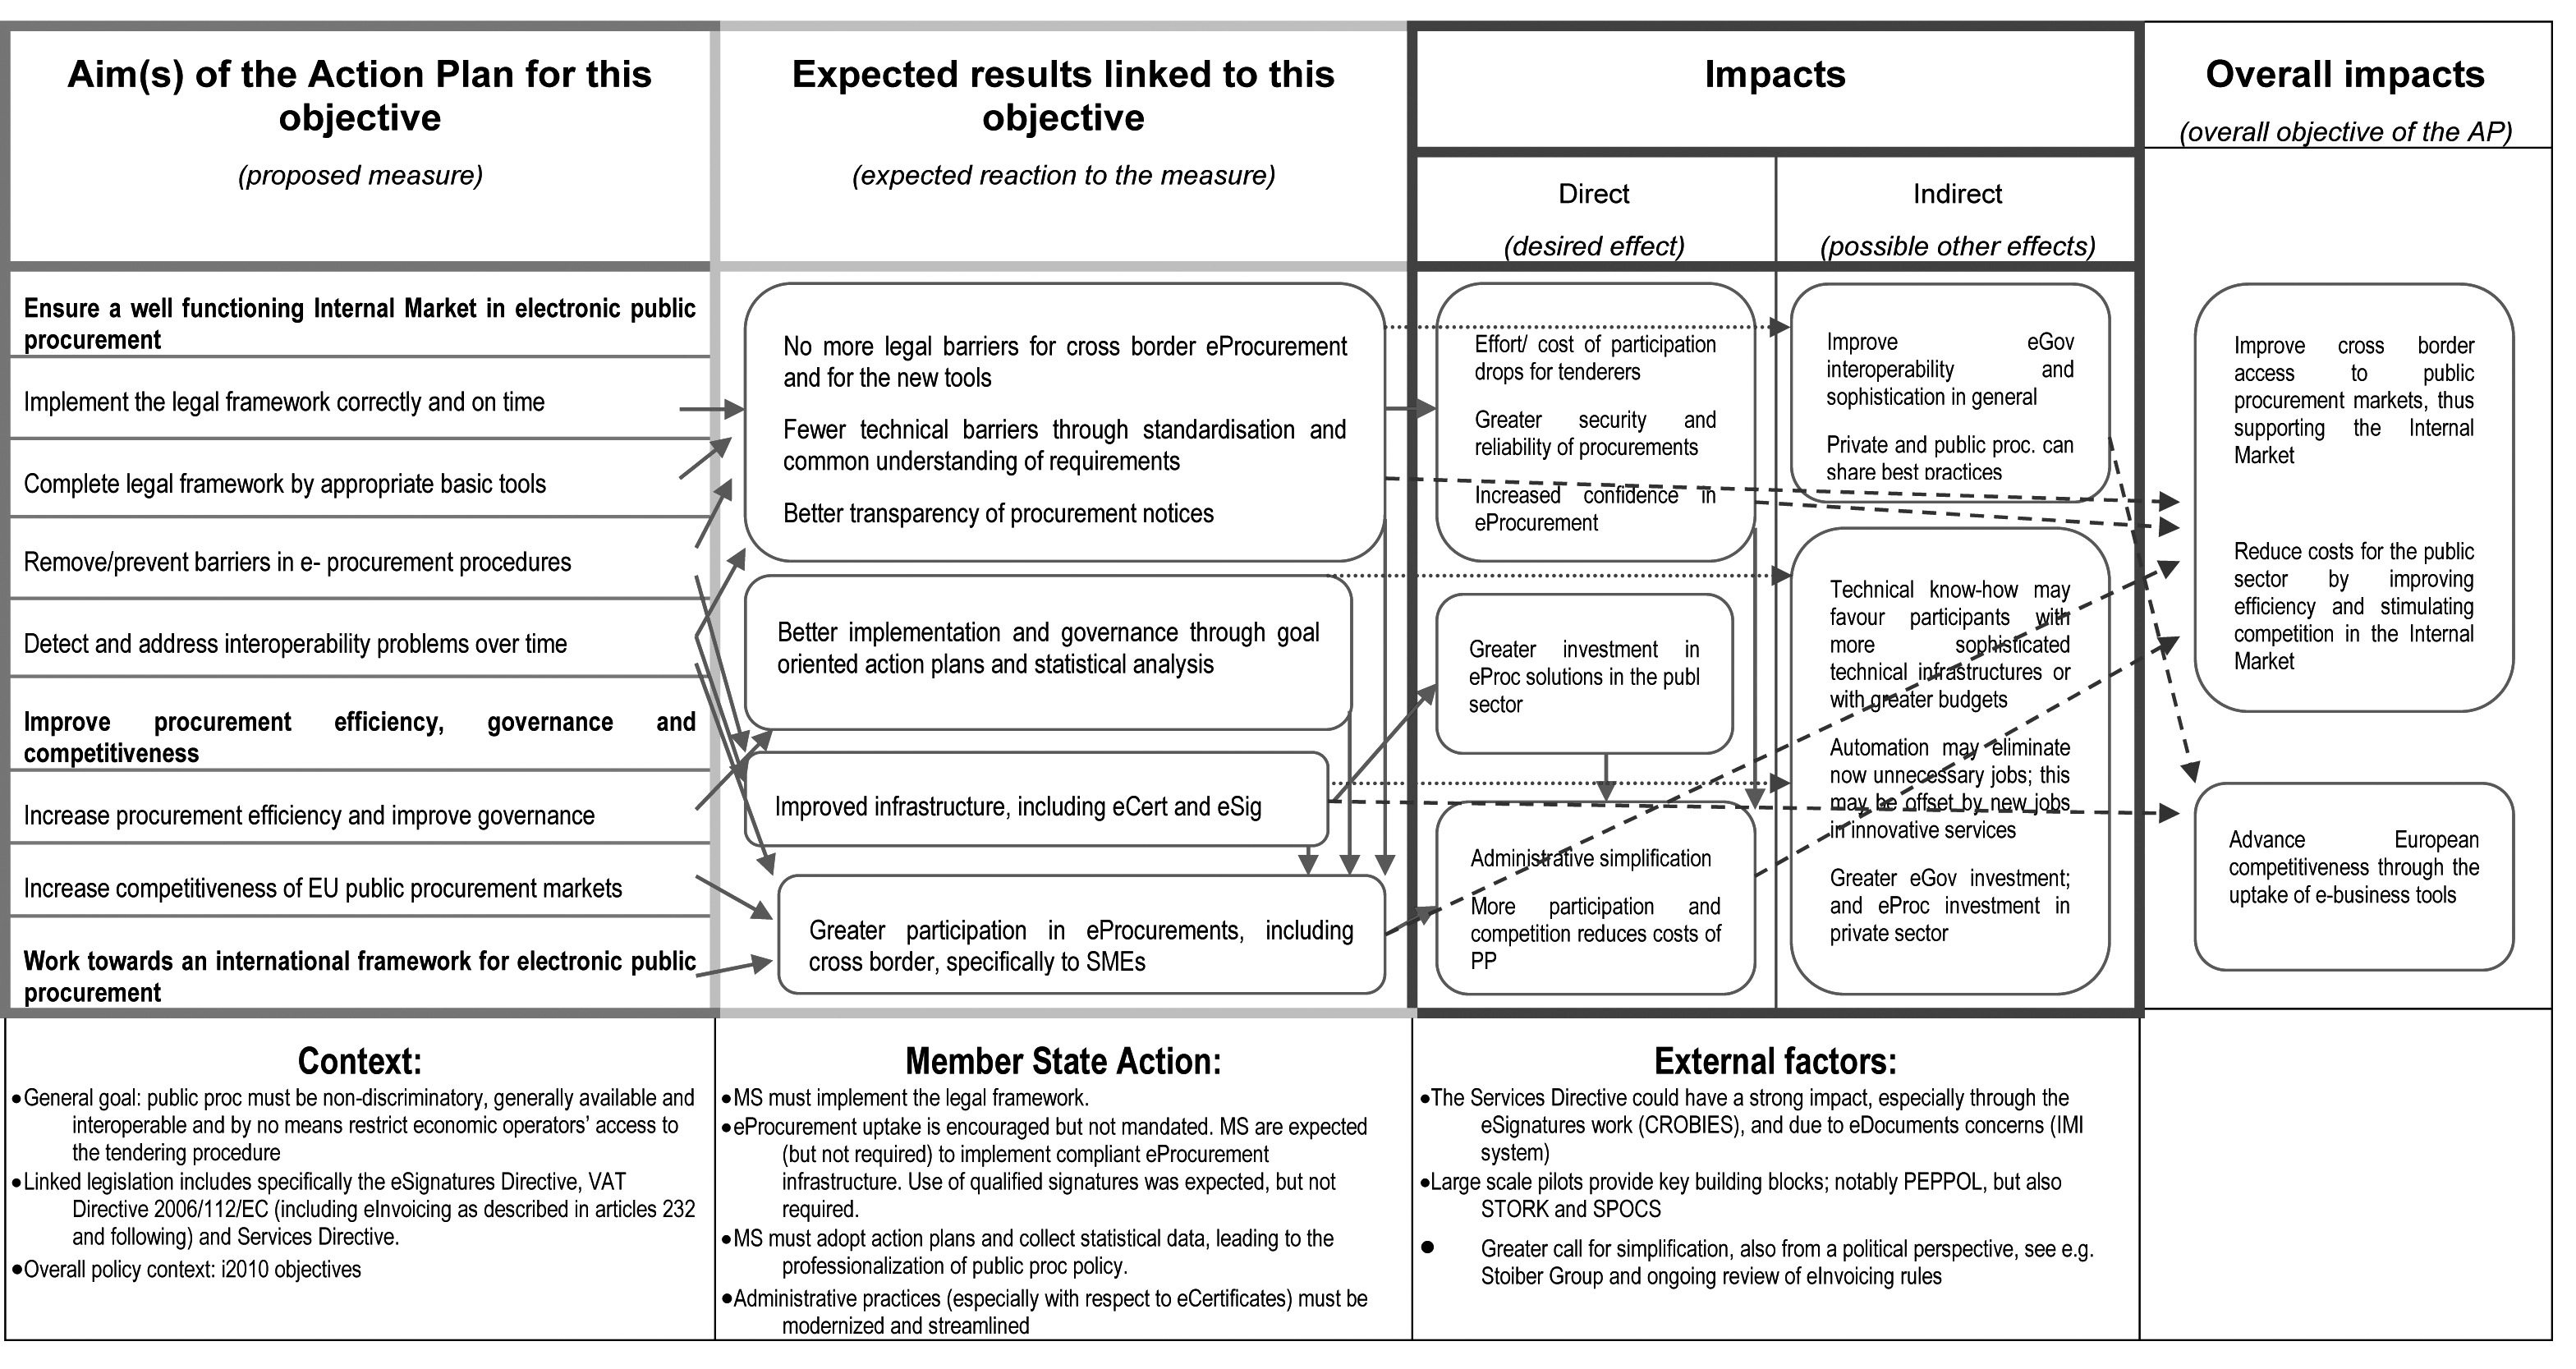
\includegraphics[width=16cm]{images/phd/eproc/ted-2}
\caption{Estrategia en e-Procurement de la Unión Europea elaborado por Siemens.}
\label{fig:ted-2}
\end{figure}

De igual forma, en este informe~\cite{siemensEval} se establecen una serie de métricas, ver Figura~\ref{fig:ted-3}, resultados e impacto, 
que deben servir como guía para las distintas acciones realizadas a nivel europeo y que
deben manifestarse en los distintos Estados Miembros.
% 
% 
\begin{figure}[!htb]
\centering
	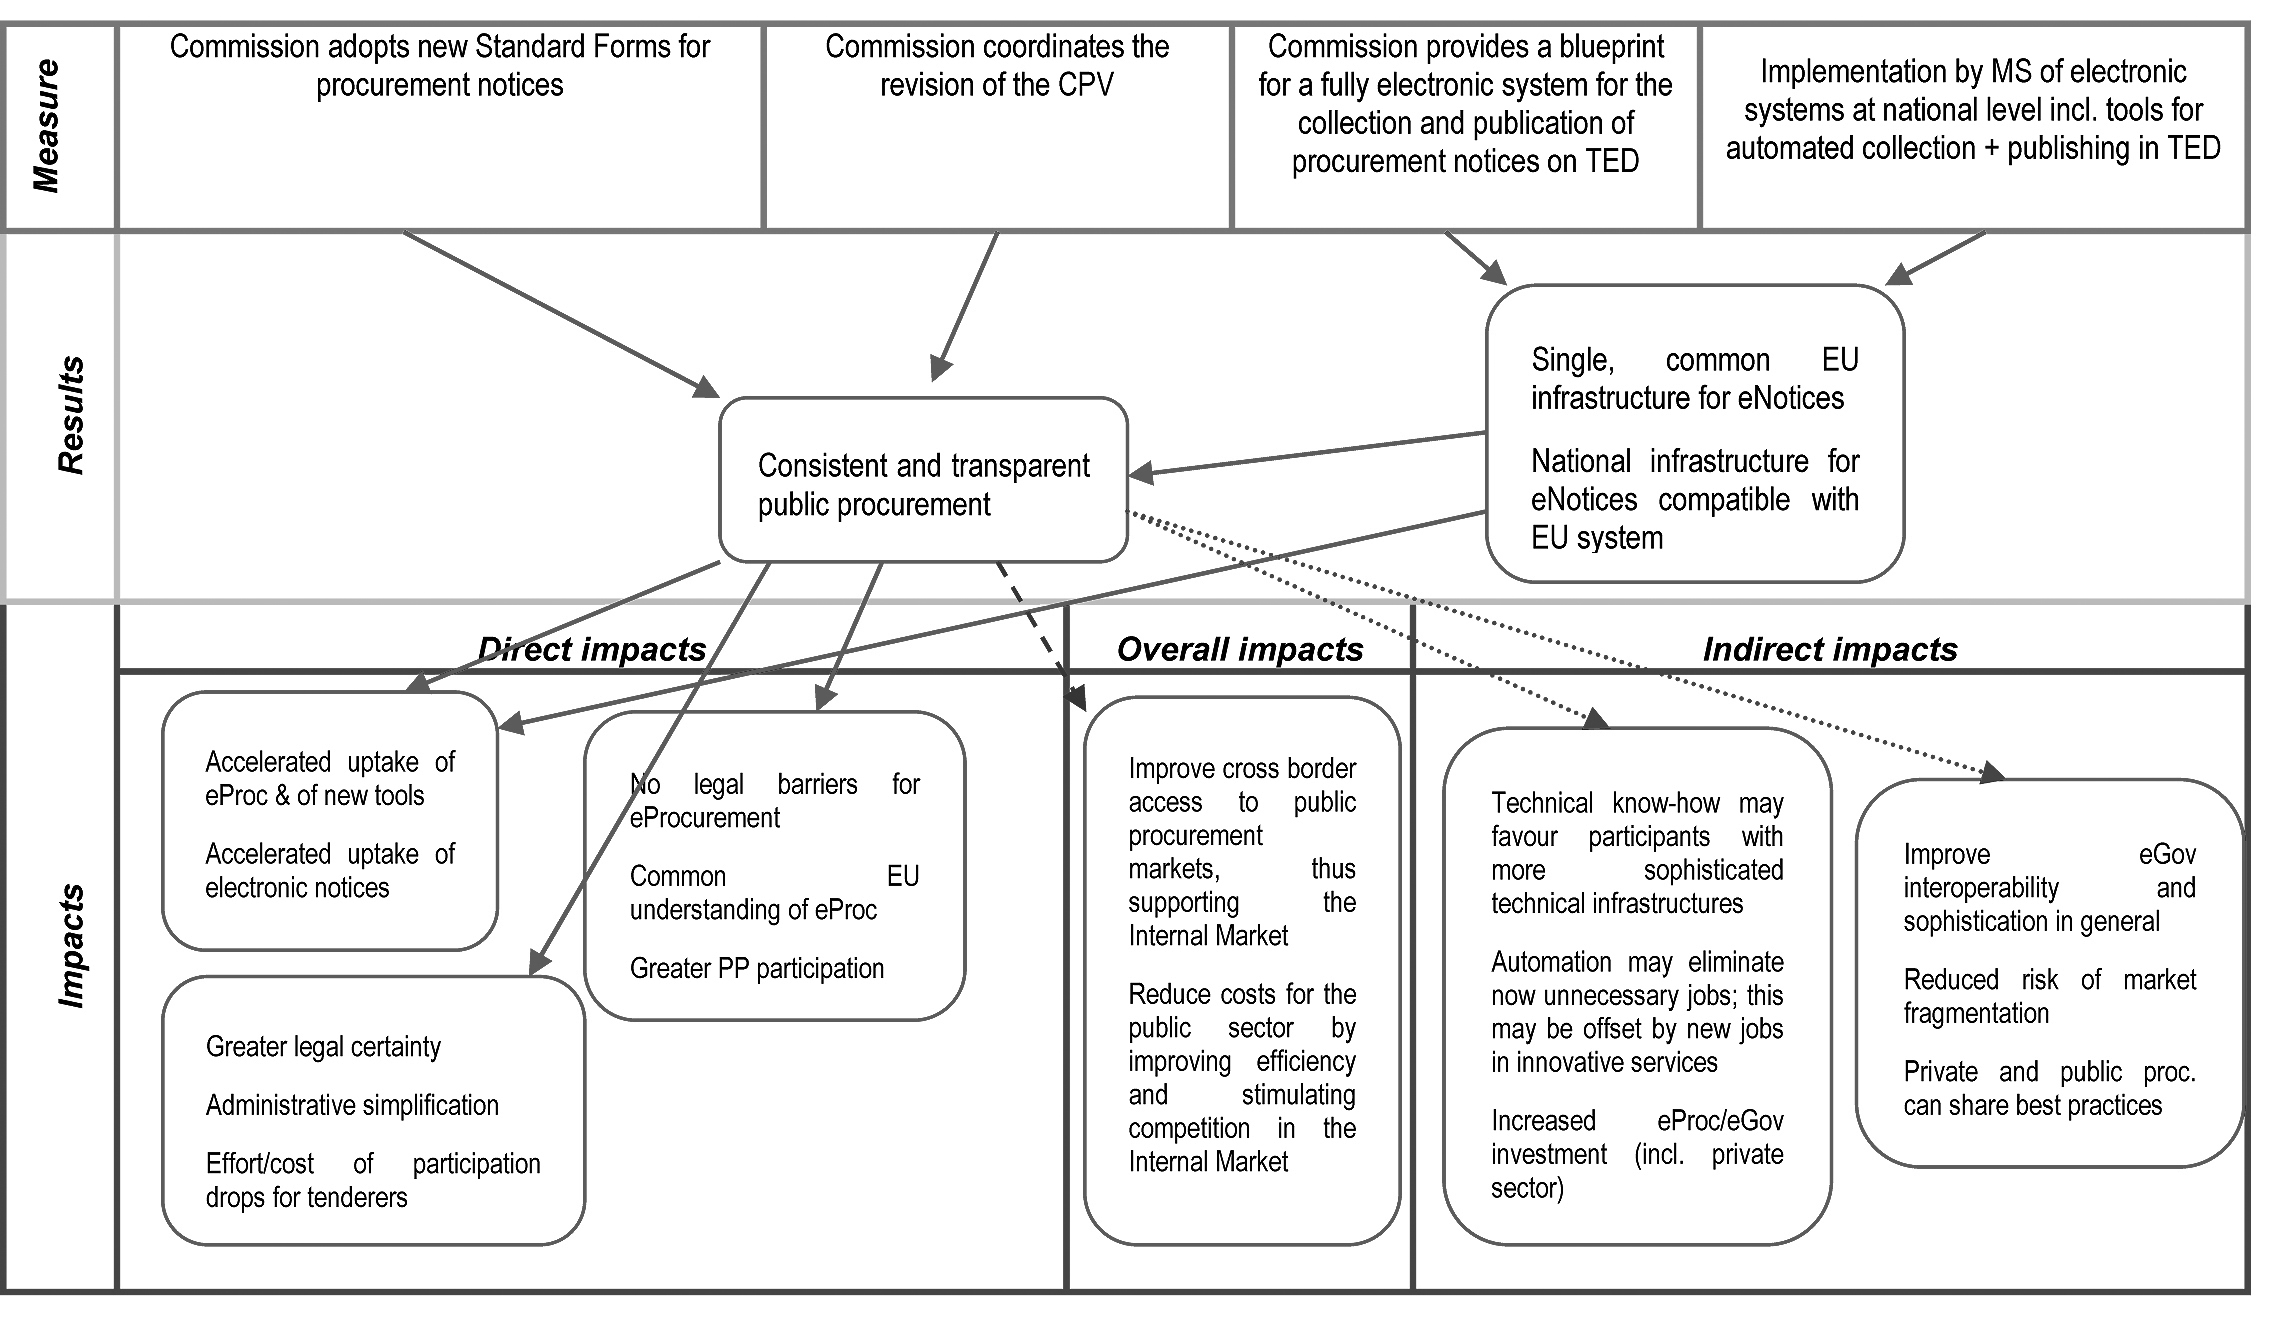
\includegraphics[width=16cm]{images/phd/eproc/ted-3}
\caption{Métricas en e-Procurement de la Unión Europea elaborado por Siemens.}
\label{fig:ted-3}
\end{figure}

A través del Plan de Acción de 2004 y de las posteriores evaluaciones continuas que se vienen realizando
en la Unión Europea, queda patente la importancia que desde las instituciones públicas se aplica
al proceso de contratación pública.
%\cleardoublepage
\subsection{Terminología}
Con el objetivo de favorecer la lectura del documento y disponer de una clara definición de cada uno
de los términos habitualmente utilizados en los procesos de contratación pública, se dispone a continuación
de una serie de definiciones (se incluyen las más importantes para el ámbito de este documento):

\begin{description}

\item [Adjudicatario (\textit{Successful tenderer}).] Empresa ganadora de un contrato público. Anteriormente en España
el proceso de adjudicación se dividía en provisional y definitivo. La diferenciación del procesos en dos partes, se 
establecía con el objetivo de comprobar si el adjudicatario cumplía las garantías necesarias.
Una vez que el proceso de selección previo se había superado, ya se establecía la formalización
del contrato con un determinado órgano y siguiendo la lista de candidatos que la Mesa de Contratación había valorado.

\item [Adjudicación (\textit{Awarding}).] Pasos que el órgano de contratación y los colectivos de soporte, 
comités de expertos o técnicos, siguen para decidir qué licitadores ofertan las mejores
opciones para ganar el contrato. Habitualmente, se utilizan diversas técnicas para
cada paso (técnica Delphi, entropía, etc.) aunque una de las máximas es obtener
la mejor relación oferta/precio, bajo las condiciones más óptimas.

\item [Agente externo.] Actor dentro del proceso de licitación que interviene en alguna
parte del proceso. Por ejemplo, en el ámbito español la Agencia Estatal de Administración Tributaria (\gls{AEAT}) o la
Tesorería General de la Seguridad Social (\gls{TGSS}), disponen de información susceptible de ser solicitada
por los sistemas de contratación electrónica de los órganos de contratación.

\item [Anuncio previo (\textit{Prior Information Notice}-\gls{PIN}).] Mensaje publicado por el órgano de contratación para informar sobre
la intención de contratar en un determinado período. Suelen contener información sobre
contratos de obras, suministros y servicios para los siguientes doce meses.

\item [Anuncio de adjudicación (\textit{Award notice}).] Mensaje publicado por el órgano de contratación mediante
los boletines oficiales como el ``Diario Oficial de la Unión Europea'' (\gls{DOUE}) y el ``Boletín
Oficial del Estado'' (\gls{BOE}), en los cuales se informa de los datos pertinentes de una
licitación y su adjudicatario. Suele corresponder a la información que se notifica
como resolución al proceso.

\item [Anuncio de licitación (\textit{Contract notice}).] Mensaje publicado por el órgano de contratación mediante
el cual se anuncia una nueva licitación, describiendo los términos legales, administrativos y
técnicos mínimos para que los empresarios expresen su interés de participación. La publicación
se realiza de forma oficial a través del \gls{DOUE}, \gls{BOE}, etc., y también forma parte del perfil
del comprador. En el ámbito español, existen otros tipos como el ``Anuncio Simplificado de Licitación'', utilizado 
en la fase de contratación específica de un Sistema Dinámico de Adquisición.

\item [Contrato (\textit{Contract}).] Documento de acuerdo entre un órgano de contratación y un licitador, que 
establece las condiciones de contratación de acuerdo a los pliegos publicados por el primero
y la oferta realizada por el segundo. Incluye firmas de las partes contratantes y toda la información
pertinente. Este documento representa la culminación del acto de licitación.

\item [Empresario (\textit{Economic operator}).] Es el ``operador económico'' que designa tanto a un ``contratista''
como a un ``proveedor'' o ``prestador de servicios''. Otros términos que se utilizan
para especificar esta figura son ``Licitador'' o ``Adjudicatario''.

\item [Espacio de trabajo de la licitación.] Espacio digital en el cual se registra toda
la documentación y aspectos relativos al proceso administrativo. Es el expediente electrónico
del proceso, que puede ser implementado mediante carpetas virtuales, registros, repositorios, etc.

\item [Licitar (\textit{Call for tenders} o \textit{tendering}).] En su acepción más amplia: acto por el cual el Estado concede contratos para la
ejecución de servicios, suministros y obras de interés público; la adjudicación definitiva de
dichos contratos puede ir precedida de un concurso o subasta en la que varias personas, físicas
o jurídicas, presentan sus cotizaciones o los precios que cobrarían por la ejecución del
contrato. También se utiliza para denominar al subconjunto de tareas ejecutadas por el empresario,
en interacción con el Órgano de contratación, destinadas a presentar una Oferta en respuesta
a un Anuncio de Licitación o una invitación a oferta.

\item [Oferta (\textit{tender}).] Documento que un empresario envía a
un órgano de contratación para licitar.

\item [Órgano de contratación (\textit{Contracting authority}).] Organizaciones, departamentos, secciones
o colegiados con la capacidad legal y estatutaria para celebrar
contratos en nombre de las entidades públicas.

\item [Perfil del contratante (\textit{Buyer profile}).] Página web en la cual se publicita toda la información
referente a los contratos de un determinado órgano de contratación.

\item [Plataforma de contratación (\textit{e-Procurement System}).] Plataforma electrónica a través de la cual se gestiona
el proceso administrativo de la contratación electrónica.

\item [Otros.] A continuación se disponen de algunos términos habitualmente utilizados
en la bibliografía relativa a contratación pública y que se consideran de interés:
acuerdo de exclusión, acuerdo marco (\textit{framework agreement}), 
agencia de garantía (\textit{guarrantee agency}), agencia registradora (\textit{registration agency}), 
artefacto (\textit{artifact}), agente externo (\textit{external agent}),
claúsulas administrativas, comité de expertos (\textit{technical committee}), 
diálogo competitivo (\textit{competitive dialogue}), expediente (\textit{procurement File}), 
garantía definitiva (\textit{tender guarantee}), invitación, mesa de contratación,
oferta indicativa, oferta temeraria, pliegos (\textit{tender information}), prescripciones técnicas,
procedimiento (\textit{procedure}): abierto, negociado, restringido, Registro Oficial de Licitadores y de Empresas Clasificadas (\gls{ROLEC} en el ámbito español), sistema dinámico de adquisición 
(\textit{dynamic purchasing system}), etc.
\end{description}

\section{Contratación Pública}
En general los participantes en un proceso de contratación pública, no difieren de la ejecución
de cualquier contrato habitual salvo que uno de los actores, como parte contratante sea la Administración Pública, 
mientras que por la parte contratada pueden distinguirse tanto a personas físicas como jurídicas con capacidad de obrar y con solvencia acreditada tanto
a nivel económico-financiero como técnico.

La Administración se estructura en diferentes órganos, compuestos por distintas unidades organizativas o 
agentes responsables de llevar a cabo las actividades de los procesos administrativos y entre ellos
el proceso de contratación pública. Para estudiar los actores participantes en el proceso de contratación, se pueden seguir diferentes criterios pero por sencillez se suele utilizar una distribución funcional
según las actividades a desarrollar por cada uno de ellos. A continuación, se detallan algunos de estos
agentes con referencia a la situación actual en el ámbito de la Administración General del Estado
en España.

\begin{description}
 \item [Contratación.] Son las entidades con capacidad para obrar un contrato. Normalmente,
se agrupan bajo el término ``Órganos de Contratación'' y dependen de la propia estructura y organización
de la Administración. Dependiendo de distintas variables como el tipo de contrato, el importe del 
mismo o el lugar de celebración, los órganos cambiarán de acuerdo a su potestad. Como ejemplo y siguiendo
la estructura y organización de la Administración General del Estado, se establecen distintas unidades
organizativas que tendrán capacidad de actuar como Órganos de Contratación. En este caso y siguiendo 
la Ley 6/1997~\cite{l6-1997}, de 14 de abril de Organización y Funcionamiento de la Administración 
General del Estado, la cual en su exposición de motivos, refiere a uno de los preceptos fundamentales
que la Constitución Española de 1978 dedica en su artículo 103 a la actividad de la Administración, así, objetividad,
generalidad, eficacia, jerarquía, descentralización, desconcentración y coordinación se constituyen como principios básicos 
de funcionamiento de la Administración.

Esta misma ley, en su artículo 3, establece que la organización y actuación de la Administración General del Estado se realizará 
con respeto al principio de legalidad y de acuerdo a los siguientes principios (entre otros):
\begin{itemize}
 \item De organización:
\begin{itemize}
 \item Jerarquía.
 \item Descentralización funcional.
 \item Desconcentración funcional y territorial
 \item Economía, suficiencia y adecuación estricta de los medios a los fines institucionales.
 \item Coordinación.
\end{itemize}
 \item De funcionamiento: 
\begin{itemize}
\item Eficacia en el cumplimiento de los objetivos fijados.
\item Eficiencia en la asignación y utilización de los recursos públicos.
\item Programación y desarrollo de objetivos y control de la gestión y de los resultados.
\item Responsabilidad por la gestión pública.
\item Racionalización y agilidad de los procedimientos administrativos y de las actividades de gestión.
\item Servicio efectivo a los ciudadanos.
\item Objetividad y transparencia de la actuación administrativa.
\end{itemize}
\end{itemize} 

También y como ejemplo, en el Capítulo II de dicha ley se establece
la ``Organización Administrativa'', tanto de la Administración General del Estado como de sus Organismos públicos. La Administración 
General del Estado responde a una organización funcional en Departamentos ministeriales y de gestión
territorial integrada en Delegaciones de Gobierno en las propias
Comunidades Autónomas. La organización de la Administración Central distingue
entre órganos superiores (S) y órganos directivos (D):
\begin{itemize}
 \item Ministros. (S)
 \item Secretarios de Estado. (S)
 \item Subsecretarios y Secretarios generales. (D)
 \item Secretarios generales técnicos y Directores generales. (D)
 \item Subdirectores generales. (D)
\end{itemize}

Esta estructuración administrativa resulta idónea para exponer una distribución modelo que dependiendo de cada
caso puede variar: Comisión Europea, Universidad, etc.

\item [Gestión.] Contribuyen al proceso de contratación pública, dando el apoyo a las actividades
de ejecución de las tareas económico-administrativas para tramitar el proceso. En general, suelen formar
parte del propio Órgano de Contratación, aunque también pueden tener carácter general, como por ejemplo la 
Dirección General del Tesoro y Política Financiera siendo los encargados en última instancia de realizar el pago
de los importes de los contratos.

\item [Control.] Se encargan de asegurar la legalidad de los procesos de contratación. En el ámbito
de la Administración General del Estado, se podría destacar la Intervención General de la Administración del Estado y el
Tribunal de Cuentas.

\item [Asesoría.] Especialistas colaboradores de la contratación para diferentes aspectos: jurídicos, técnicos, económicos u 
otros que pudieran requerirse. Siguiendo con el ejemplo anterior, y en general: la Junta Consultiva de Contratación Administrativa o 
los Servicios Jurídicos del Estado, por otra parte, en particular podríamos citar: las Oficinas Técnicas de Supervisión
de Proyectos o la Comisión Interministerial de Adquisición de Bienes y Servicios Informáticos (CIABSI).


\item [Publicidad.] Canales de comunicación para hacer públicas las convocatorias y los procedimientos de contratación. En el 
ámbito de la Administración General del Estado podemos citar el BOE o la Plataforma
de Contratación del Estado. En el ámbito europeo hay que mencionar el DOUE, \textit{Tenders Electronic Daily} (\gls{TED}) 
o el Sistema de Información para la contratación pública europea (SIMAP).


\item [Otros.] Funciones de carácter transversal, como las obligaciones tributarias o de seguridad social. Continuando con el ejemplo citado, 
la Agencia Tributaria o la Tesorería de la Seguridad Social serían agentes participantes que dan soporte a las actividades derivadas de la contratación pública.
\end{description}


\subsection{Ejemplo: la Administración General del Estado en España}
En esta sección se recoge parte de la casuística implicada en un proceso de contratación
pública con la Administración General del Estado, con el objetivo de mostrar las actividades
que se han de desarrollar y desvelando algunas de las interacciones que surgen entre los distintos
agentes con las consiguientes necesidades de interoperabilidad e integración.

Actualmente cada Comunidad Autónoma tiene su propia plataforma de contratación y perfil
del contratante, ver Tabla~\ref{table:plataformas}, en la cual se pueden realizar las operaciones del proceso de contratación pública 
electrónica. En muchos de los casos están enlazadas con la Plataforma de Contratación del Estado~\cite{PlataformaContratacionEstado}
y siguen sus estándares como ``Componentes y Documentos Interoperables para la Contratación Electrónica'' (\gls{CODICE}) 
para la gestión de la información y documentación generada a lo largo del proceso. Evidentemente y dependiendo de 
la capacidad de cada órgano de contratación podrán desplegar su propia plataforma, la administración en España sigue un modelo
descentralizado y coordinado desde la Administración General del Estado, o bien utilizar la infraestructura común.
%Comunidad, Plataforma

\begin{longtable}[c]{|p{7cm}|p{8cm}|} 
\hline
  \textbf{Comunidad Autónoma} & \textbf{Plataforma de Contratación} \\\hline
\endhead
Andalucía & \url{http://www.juntadeandalucia.es/contratacion} \\ \hline
Aragón & \url{http://portal.aragon.es/portal/page/portal/CPUBLICA#} \\ \hline
Castilla y León & \url{http://www.jcyl.es/web/jcyl/Portada/es/Plantilla100/1246947706077/_/_/_} \\ \hline
Castilla La Mancha & \url{http://pagina.jccm.es/contratacion/} \\ \hline
Cantabria  & \url{https://aplicaciones5.cantabria.es/PerfilContratante} \\ \hline
Canarias & \url{http://www.gobcan.es/perfildelcontratante/contenido} \\ \hline
Cataluña & \url{https://contractaciopublica.gencat.cat} \\ \hline
Región de Murcia & \url{http://www.carm.es/web/pagina?IDCONTENIDO=6427&IDTIPO=100} \\ \hline
Comunidad de Madrid & \url{http://www.madrid.org/cs/Satellite?cid=1203334374251&language=es&pagename=PortalContratacion/Page/PCON_contenidoFinal} \\ \hline
Comunidad Valenciana & \url{https://www.contratacion.gva.es/WebContrataP} \\ \hline
Cdad. Foral de Navarra & \url{http://www.navarra.es/home_es/Servicios/Portal+contrataciones/} \\ \hline
Extremadura & \url{https://contratacion.juntaextremadura.net} \\ \hline
Galicia & \url{http://www.contratosdegalicia.es/} \\ \hline
Illes Balears & \url{http://www.plataformadecontractacio.caib.es/} \\ \hline
La Rioja & \url{http://www.larioja.org/npRioja/default/defaultpage.jsp?idtab=26275} \\ \hline
Principado de Asturias & \url{https://sede.asturias.es} \\ \hline
País Vasco & \url{http://www.euskadi.net/r33-2288/es/contenidos/informacion/perfil_anuncios/} \\ \hline
 \hline
\caption{Plataformas de Contratación en las Comunidades Autónomas.}\label{table:plataformas}\\    
\end{longtable}

En estas plataformas las operaciones a realizar, los idiomas disponibles, etc., son variados, si además se amplia el rango
de órganos de contratación a Universidades, Ayuntamientos, Parroquias Rurales, Mancomunidades, etc.,  y ahora se proyecta
a nivel europeo es factible advertir la diversificación y la replicación de esfuerzos que se están efectuando en este ámbito. 
Por ello, iniciativas como la Plataforma de Contratación del Estado o \gls{TED} ayudan a unificar y facilitar el acceso a las distintas fases del proceso
de contratación pública.

\section{Contratación Pública Electrónica: \textit{e-Procurement}}
El término \eproc~\cite{Podlogar2007} se utiliza para designar el uso de medios y tecnologías electrónicos para llevar a cabo
las operaciones y comunicaciones relacionadas con la contratación pública, y en general para todos aquellos procesos~\cite{DBLP:journals/tcci/Alor-HernandezAJPRMBG10}
en los que participen proveedores y consumidores de un cierto servicio o producto. En el caso particular de las Administraciones
Públicas se utiliza esta terminología para definir las operaciones llevadas a cabo para adquirir bienes o servicios mediante
distintos métodos: contratación directa, centrales de contratación, contratos de urgencia y emergencia, etc.

La importancia del proceso de contratación pública electrónica, va más allá de la simple transición del papel ya que puede
aportar mejoras relevantes en eficiencia de las adquisiciones, gestión global del proceso de contratación pública y en general, 
al funcionamiento de los mercados de las administraciones.

La tendencia actual para acelerar la implantación de procesos de contratación, se alinea con las directrices de impulso de la administración
electrónica como camino para la transformación del funcionamiento de la Administración Pública y la prestación de servicios. En este sentido,
la Agenda Digital de la Comisión Europea está trabajando en una guía o ``libro blanco'', para fijar las medidas que aseguren el despliegue
de una infraestructura integradora de la contratación pública para atender las necesidades de los distintos países. Como primer paso para la 
consecución de este gran objetivo, se ha elaborado una declaración de intenciones a través de un ``libro verde'' en el cual se pone de manifiesto el ambicioso objetivo
de uso de las TICs en este dominio de la Administración Pública. 

El nacimiento de esta propuesta está fechada en el año 2005 cuando los Ministros de la Unión Europea manifestaron su deseo de conseguir ``en el año 2010,
que como mínimo el $50$\%  de toda la contratación pública que rebase el umbral de contratación pública de la Unión \gls{Europea} se lleve a cabo
por medios electrónicos''. Teniendo presente esta intención se modificó la legislación pertinente y se puso en práctica el ``Plan 
de Acción sobre Contratación Electrónica''~\cite{plan2004} en el año 2004. Aunque desde un punto de vista teórico se han sentado las bases para la contratación
pública electrónica, la realidad es que el grado de implantación efectiva es muy inferior al esperado, ya que la complejidad subyacente,
ver Figura~\ref{fig:e-proc-complexity}, abarca distintos niveles: técnico, logístico y administrativo. Siguiendo la evaluación realizada por la Comisión, se señala que al
menos el $5\%$ del presupuesto total destinado a la contratación en los \gls{Estados} Miembros que iniciaron esta línea de acción se adjudica
por canales electrónicos.

\begin{figure}[!htb]
\centering
	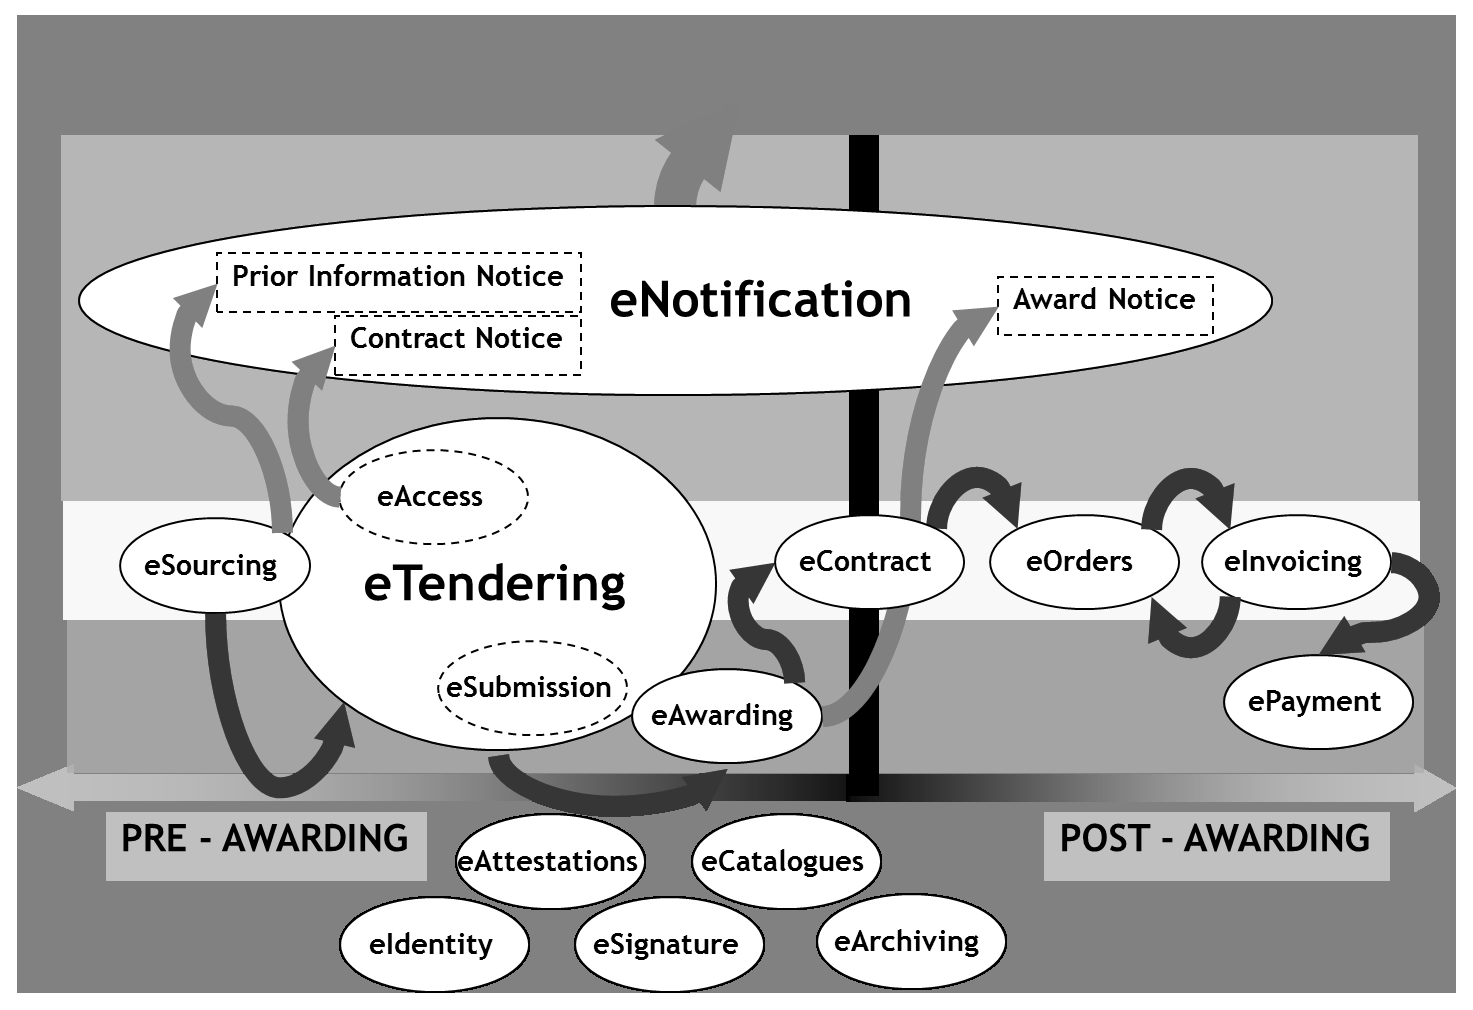
\includegraphics[width=16cm]{images/phd/eproc/e-proc-complexity}
\caption{Diagrama de Complejidad y Fases de e-Procurement por la Unión Europea.}
\label{fig:e-proc-complexity}
\end{figure}

Ahora bien, el crecimiento de este porcentaje depende en buena medida de que la contratación electrónica sea implantada a todos los niveles
administrativos (local, regional y estatal), para ello se debe contar con la tecnología necesaria, en muchos casos ya disponible, así como
de plataformas de contratación que se puedan integrar a nivel operativo para que el tráfico a través de las mismas genere la masa
crítica suficiente como para alcanzar los requisitos fijados por la Comisión para lograr la innovación en este proceso. Además de incrementar el uso
de medios electrónicos en la contratación pública, surge la oportunidad de armonizar este proceso administrativo de forma transfronteriza
de tal forma que se impulse la participación de las empresas en procesos de contratación pública más allá de su región de origen, fomentando 
así la competitividad y mejorando tanto los productos como los servicios a contratar y por extensión potenciando tanto las posibilidades
de las entidades dispuestas a licitar, como los servicios prestados por la propia administración.


\subsection{Definición de Contratación Electrónica}
Siguiendo la definición realizada por la Unión Europea~\cite{e-Proc-green-paper}, se puede definir contratación electrónica como:

\textit{La contratación electrónica es un término general utilizado para designar la sustitución de los
procedimientos basados en soporte de papel por el tratamiento y la comunicación mediante
TIC a lo largo de toda la cadena de contratación pública. Supone la introducción de
procedimientos electrónicos para sustentar las distintas fases del proceso de contratación, es
decir, publicación de los anuncios de licitación, suministro del pliego de condiciones,
presentación de ofertas, evaluación, adjudicación, pedido, facturación y pago.}

\textit{Los procedimientos vinculados a la facturación y el pago (posteriores a la adjudicación) no
son específicos de la contratación; por tanto, es posible aplicar en el ámbito de la contratación
pública electrónica soluciones desarrolladas para un mercado más amplio (de empresa a
empresa) 6 . No obstante, en algunas fases (notificación, presentación de propuestas,
valoración y pedido) se requieren soluciones específicas. Las fases de presentación,
valoración y pedido son las más arduas ya que exigen la aplicación de una serie de protocolos
y normas consensuados para organizar el intercambio de documentos complejos, así como la
interacción entre el comprador público y los proveedores.}

No obstante, consultando la actividad propuesta por la Unión Europea para la contratación electrónica
se han fijado algunos aspectos que deberán todavía coexistir de forma no automatizada. Es el caso
de la documentación de procesos de contratación complejos como pueden ser los planos y diseños
de obras, ya que es necesario disponer de los originales de forma impresa y normalizados para poder ser consultados por
los propios expertos de la administración y realizar las validaciones pertinentes. 

Ahora bien para dar cabida a la contratación pública electrónica se ha necesitado un esfuerzo por parte
de las diferentes Administraciones para la creación de portales en los cuales contener los anuncios de licitación y facilitar
el acceso a la descripción de los mismos, y más en particular a los pliegos de condiciones técnicas y económicas. 
De esta forma, se da un paso hacia delante al disponer de un servicio público electrónico de ``principio a fin''. 
Este tipo de plataformas han sido denominadas como ``plataformas de contratación electrónica'', como ejemplo
podemos citar la ``Plataforma de Contratación del Estado''~\cite{PlataformaContratacionEstado} entre otras. 
También y de forma obligatoria, aquellos entes que quieran hacer uso de la contratación pública electrónica deben 
publicar su ``Perfil de Contratante''~\cite{PerfilContratante}. En el caso de España, existen otras características que impulsarán la 
contratación pública electrónica como la factura electrónica~\cite{FacturaElectronica}.

Por otra parte, el proceso de contratación pública y en concreto el que concierne a la contratación pública electrónica cuenta 
con distintas fases~\cite{siemensEval} con diferentes objetivos y que se deben abordar en un contexto común, definiendo 
para cada uno de ellos sus características.  A continuación, se disponen de las distintas fases identificadas, ver Figura~\ref{fig:ted-1}, 
por la Comisión en este ámbito y que sirven para focalizar el objetivo de este documento.


\begin{figure}[!htb]
\centering
	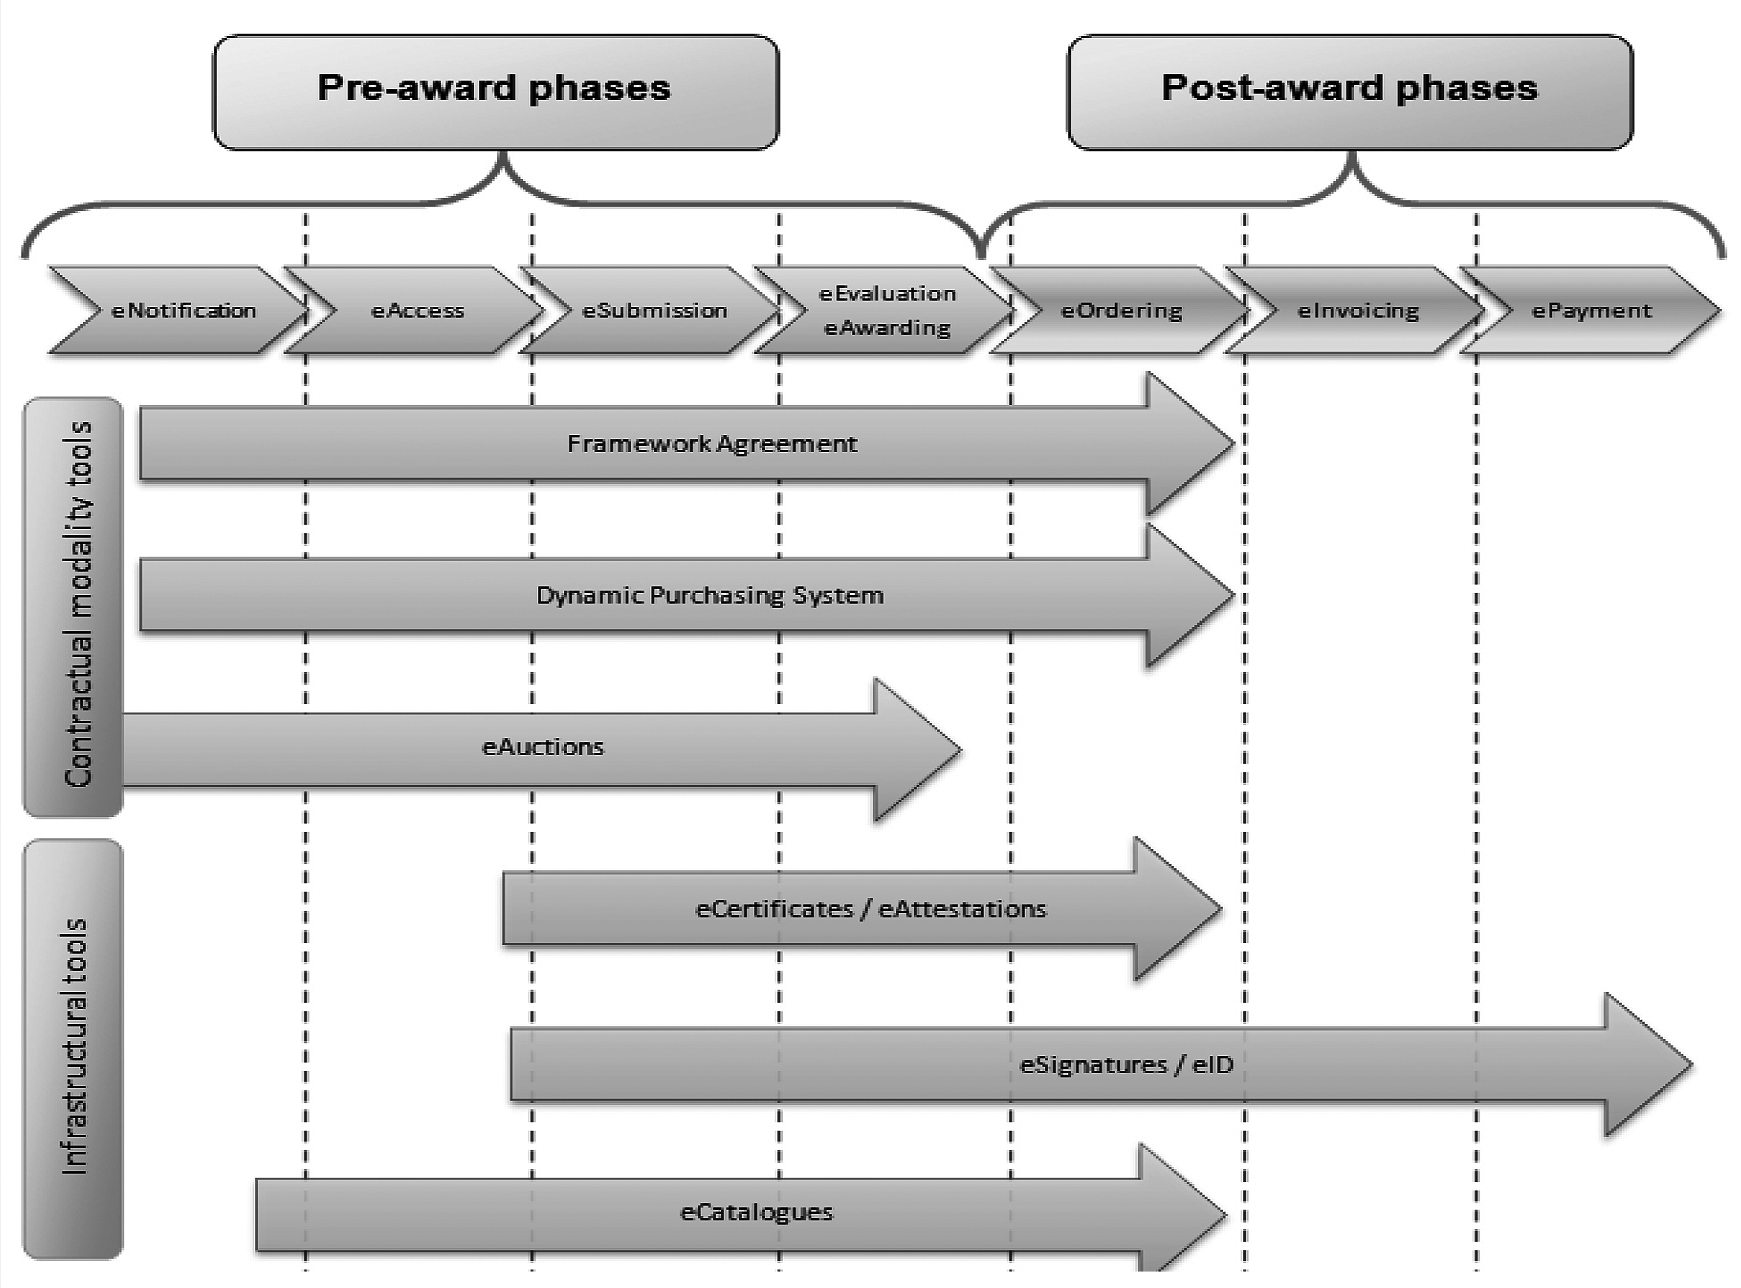
\includegraphics[width=16cm]{images/phd/eproc/ted-1}
\caption{Fases de e-Procurement definidas por la Comisión Europea.}
\label{fig:ted-1}
\end{figure}


\begin{description}

 \item [\textit{eNotification}.] Esta fase cubre la publicación de anuncios de licitación. Se trata
de un proceso unilateral que conlleva la comunicación entre órgano de contratación y el sistema
de publicación. Es el primer paso para facilitar el acceso a la información contenida
en los anuncios de licitación. El principal desafío de esta fase es realizar la publicación
de la información de la forma más estandarizada posible. Actualmente, se utiliza XML como 
formato de publicación y mediante herramientas como eSenders es posible enviar la información
a través de distintos canales como fax o correo electrónico. Los órganos de contratación 
se encargan de esta tarea buscando agilizar el proceso de publicación y asegurando
que no existan errores. A nivel europeo, en el año 2009, alrededor del $89\%$ de los anuncios de licitación
utilizan un medio electrónico para ser publicados. En la Figura~\ref{fig:circa-1}, se puede ver el uso 
de los medios para la publicación de anuncios realizados por los distintos Estados Miembros de forma agregada. Por ejemplo y comparando algunos países, 
en España sería un $88,8\%$  (ver Figura~\ref{fig:circa-6}) y en Alemania un $82,9\%$ (ver Figura~\ref{fig:circa-5}).


\begin{figure}[!htb]
\centering
	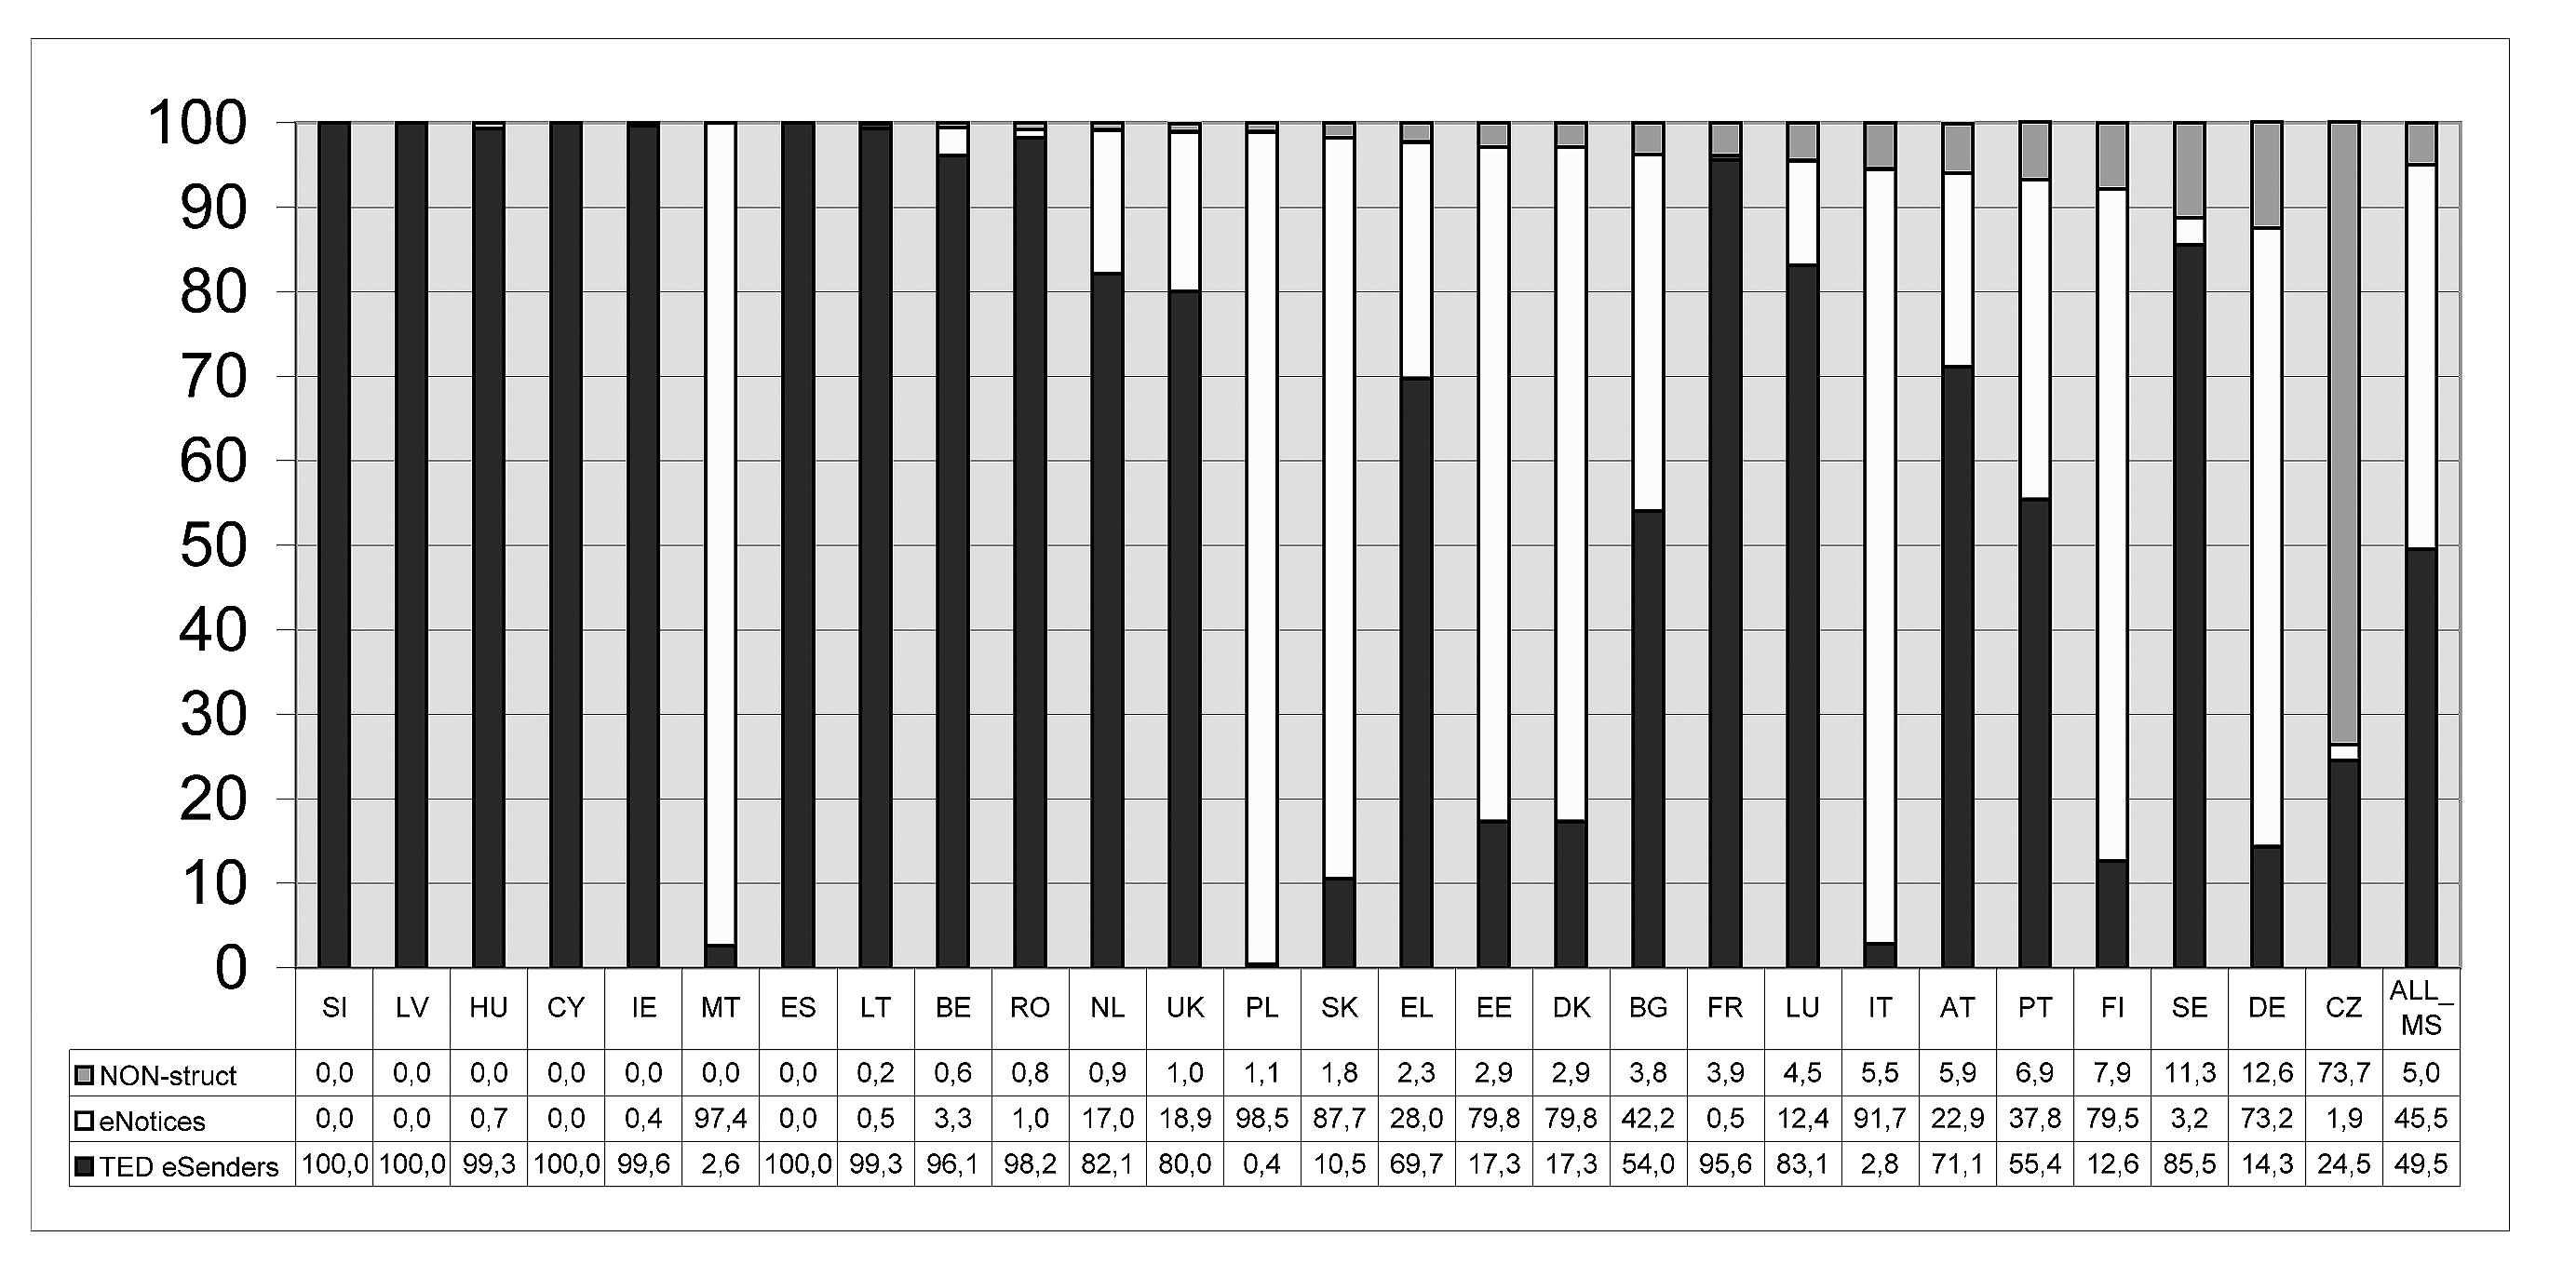
\includegraphics[width=16cm]{images/phd/eproc/circa-1}
\caption{Porcentaje y Tipo de Publicación de Anuncios de Licitación en TED.}
\label{fig:circa-1}
\end{figure}


\begin{figure}[!htb]
\centering
	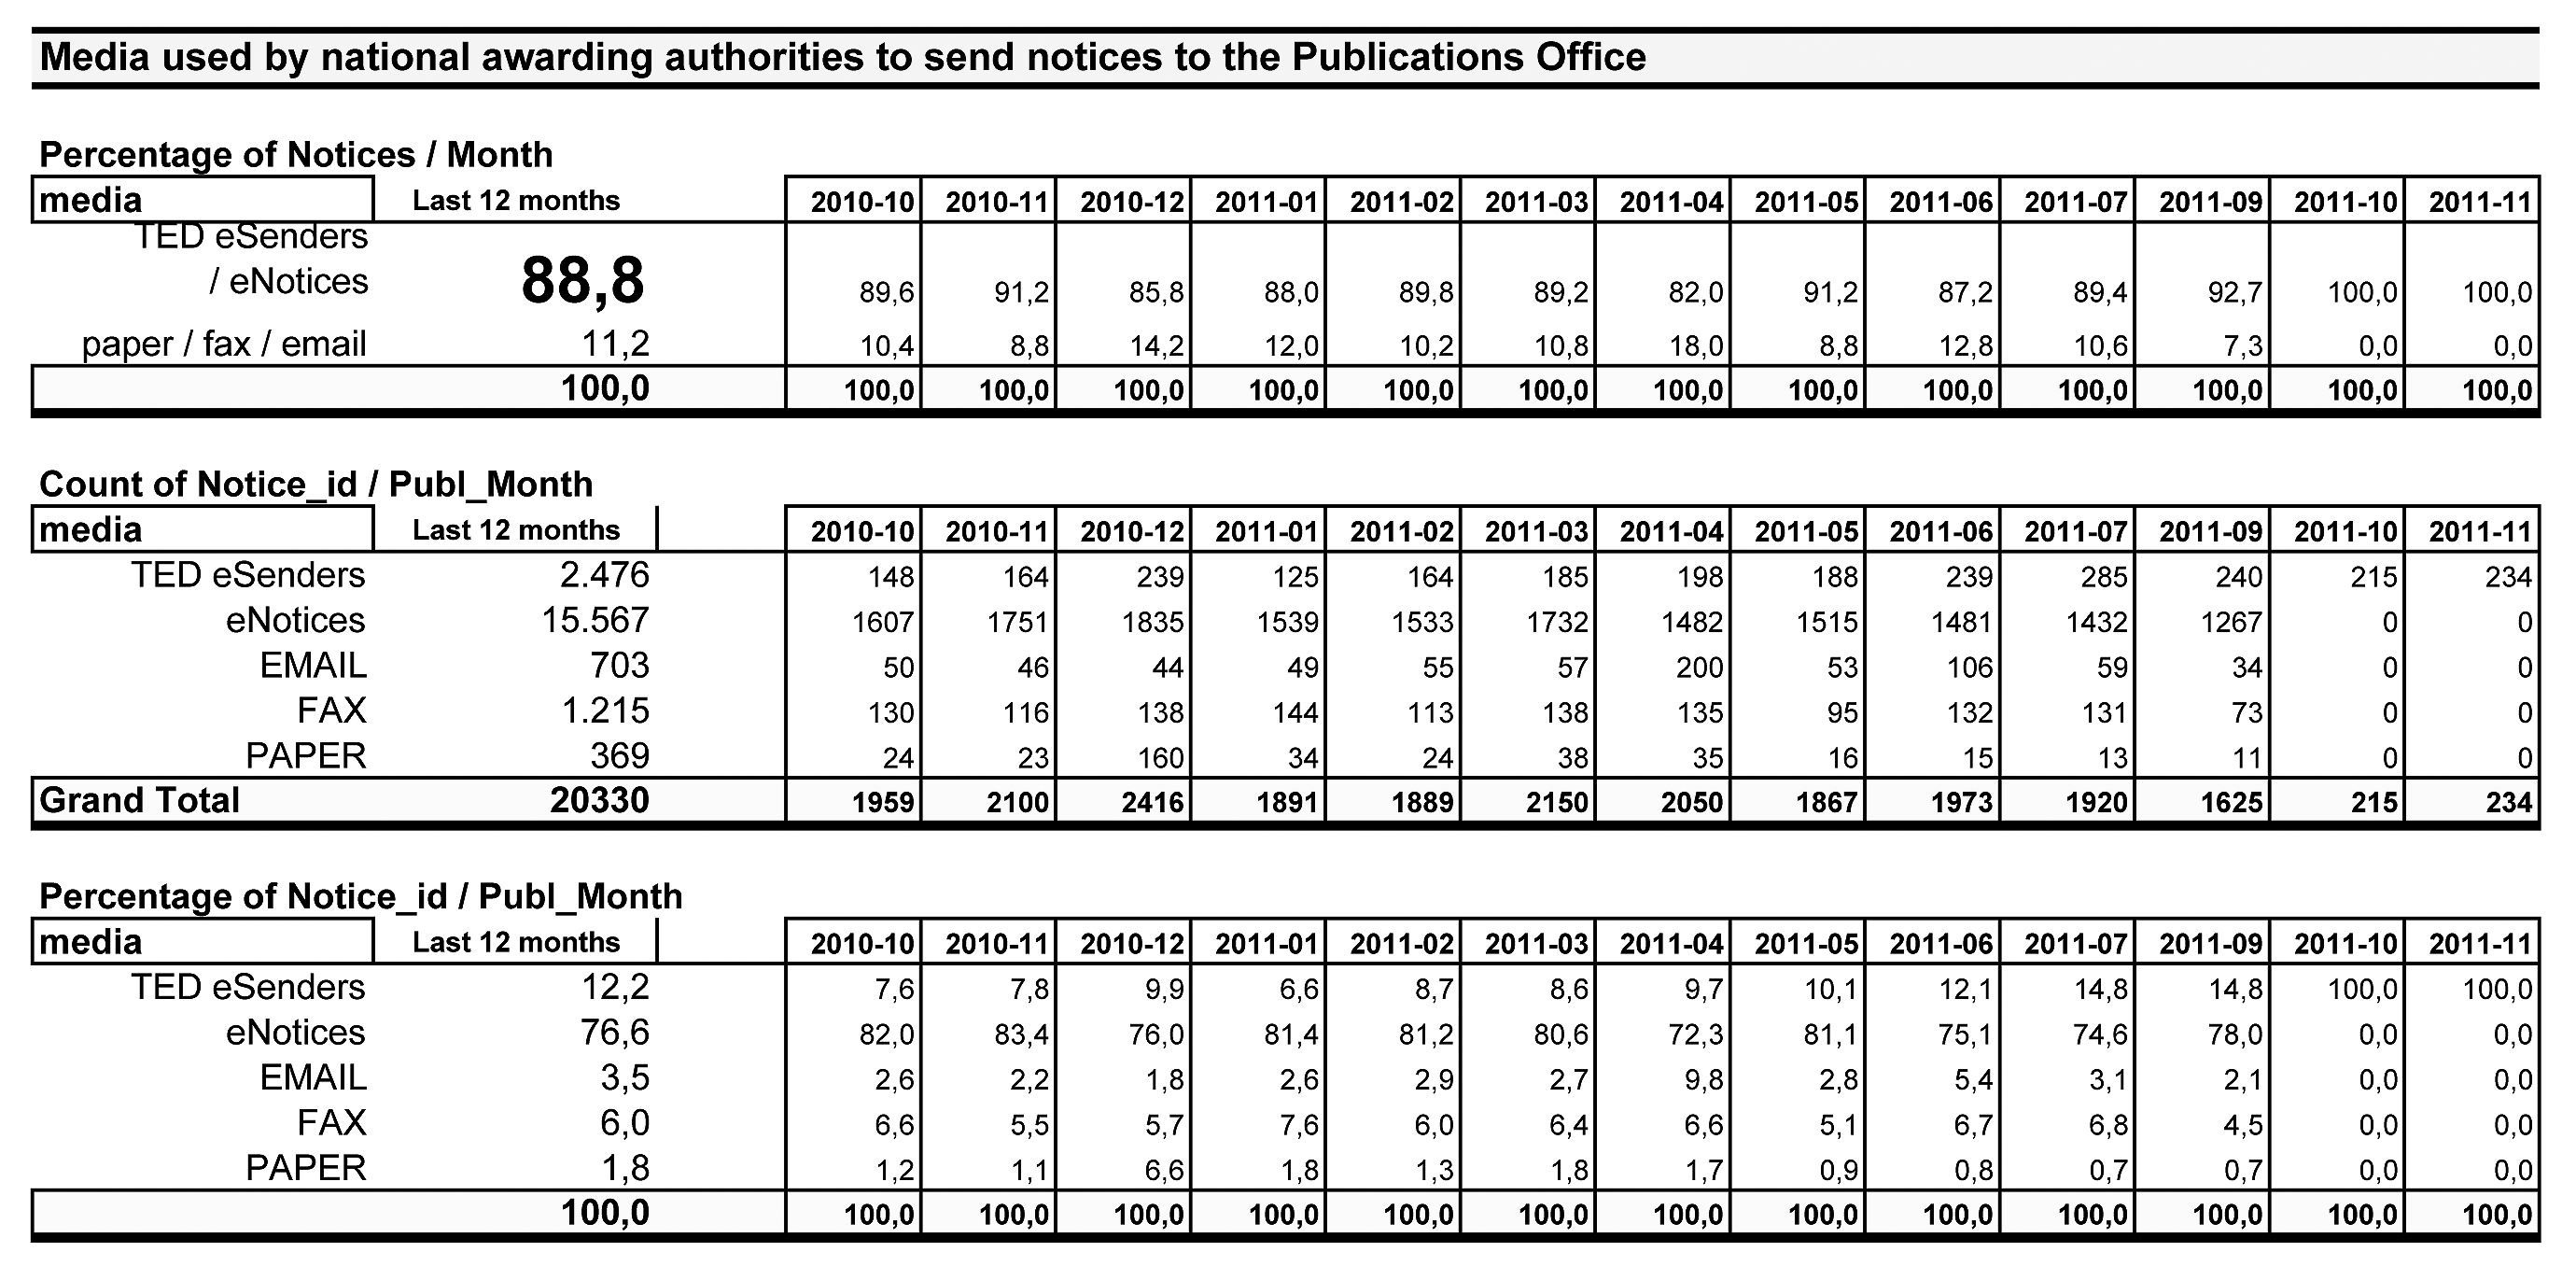
\includegraphics[width=16cm]{images/phd/eproc/circa-6}
\caption{Porcentaje y Tipo de Publicación de Anuncios de Licitación en TED de España.}
\label{fig:circa-6}
\end{figure}


 \begin{figure}[!htb]
\centering
	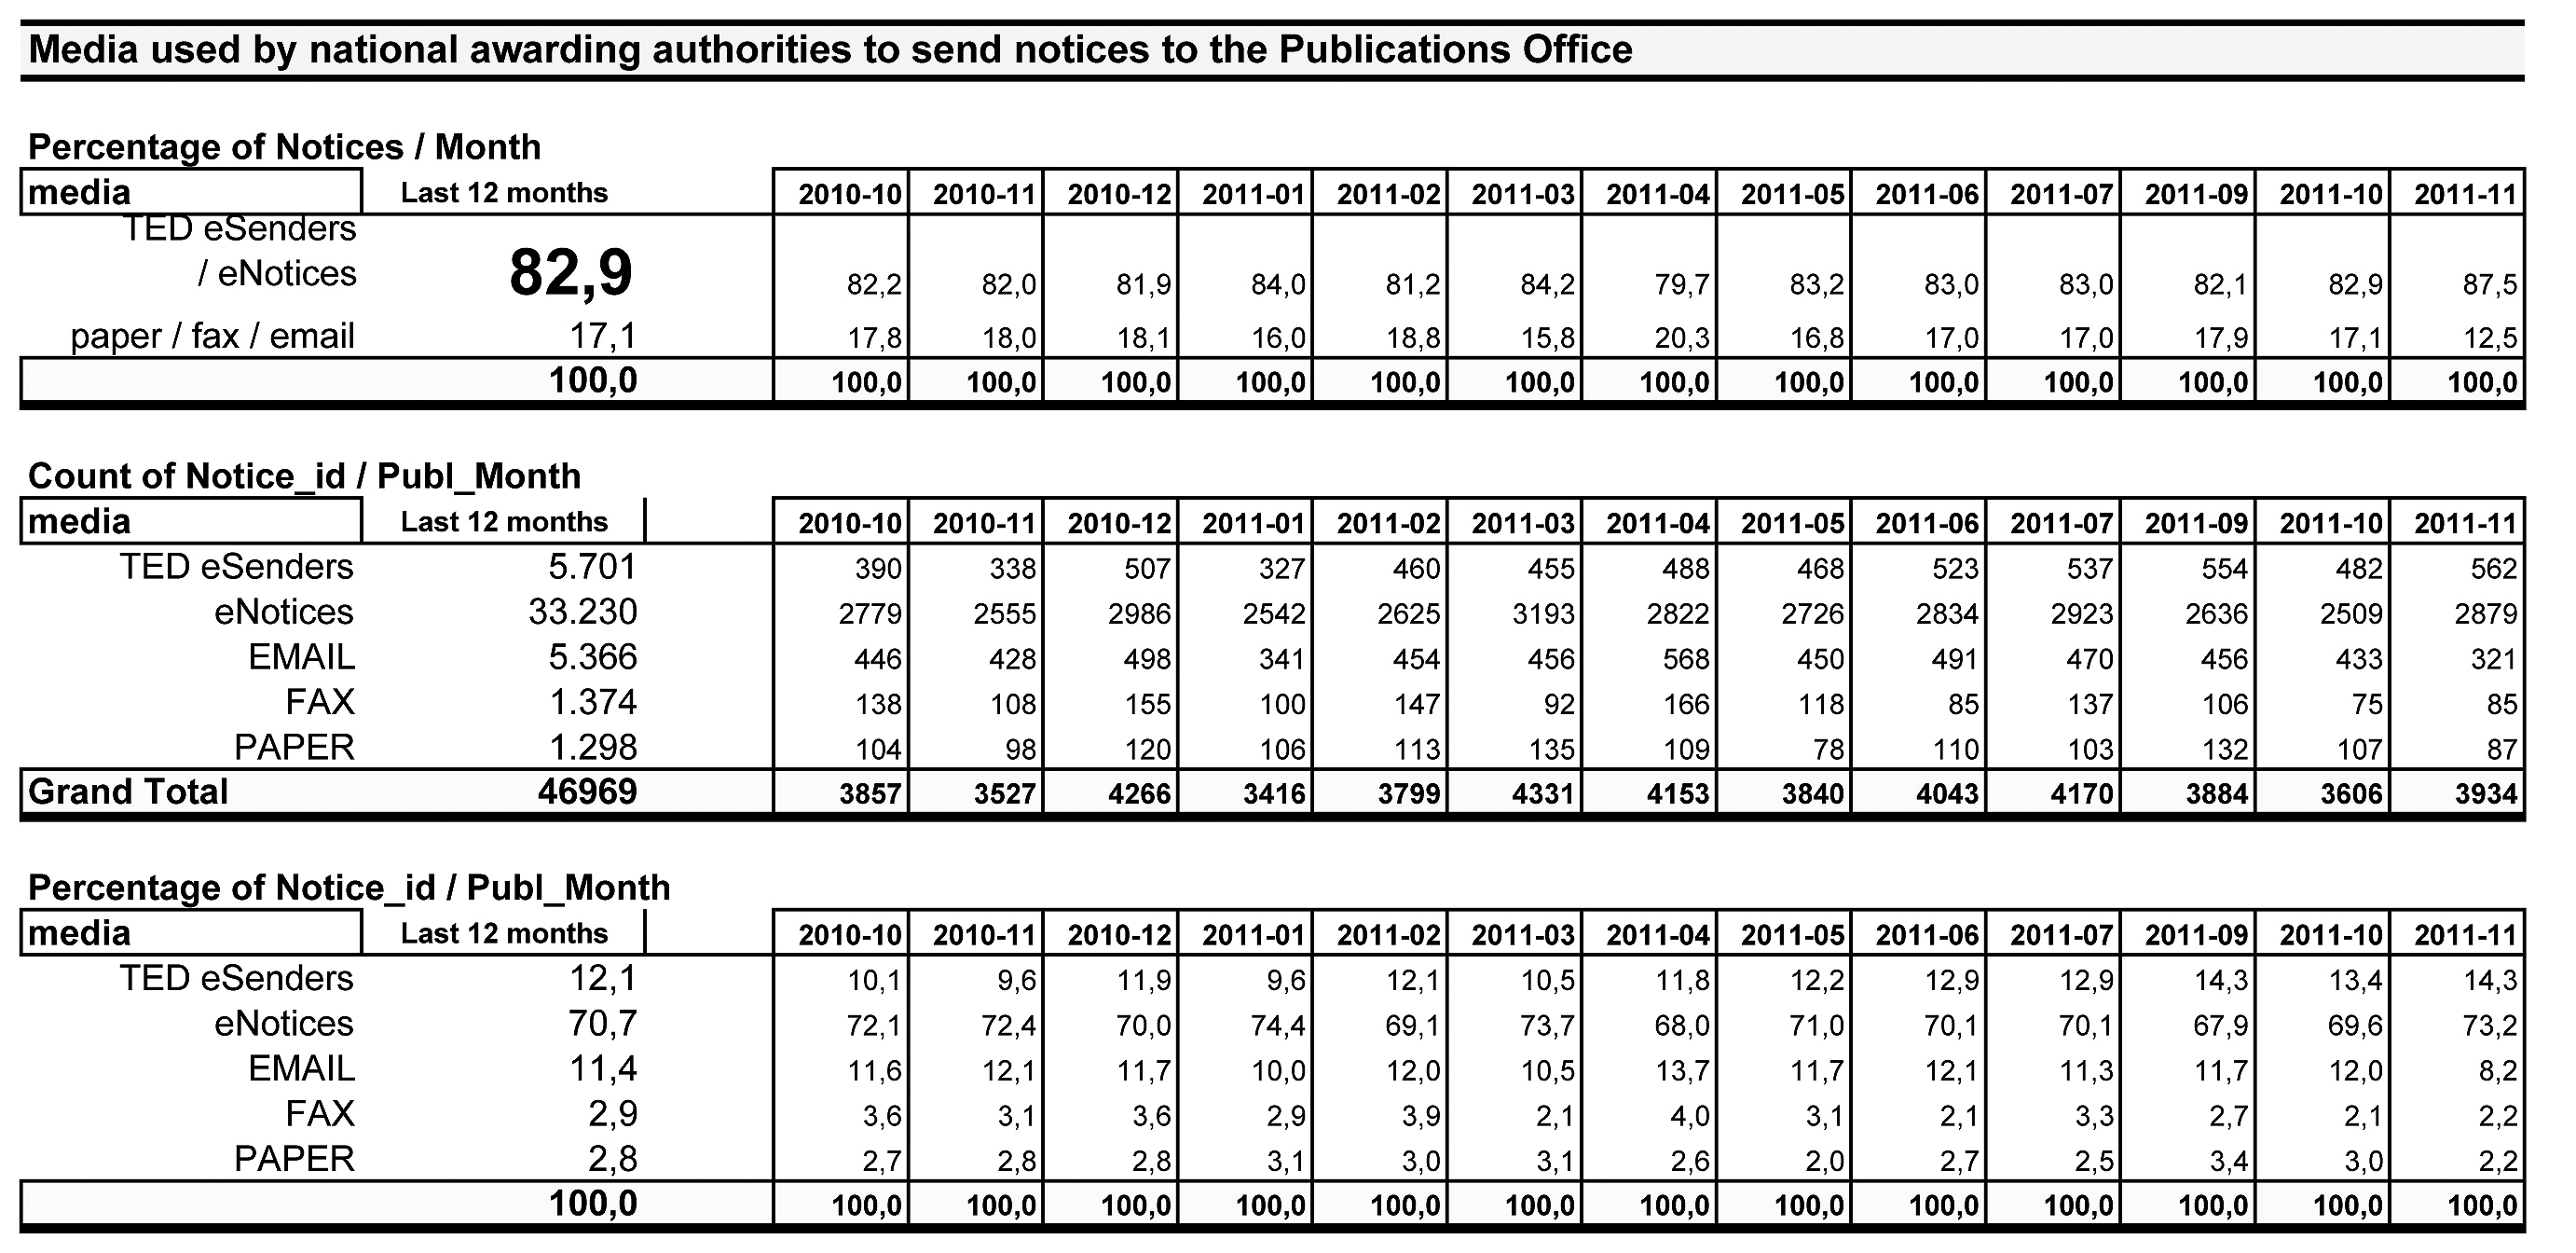
\includegraphics[width=16cm]{images/phd/eproc/circa-5}
\caption{Porcentaje y Tipo de Publicación de Anuncios de Licitación en TED de Alemania.}
\label{fig:circa-5}
\end{figure}


\item [\textit{eAccess}.] Esta fase cubre la habilidad de obtener copias de cualquier documento del 
proceso de contratación electrónica, incluyendo los anuncios de licitación. Los medios habituales
para posibilitar el acceso son la publicación a través de distintos sitios web o mediante correo
electrónico. Se trata igualmente de un proceso unilateral, cuya relevancia radica
en que las buenas prácticas y la estandarización deben estar presentes como puntos clave
para facilitar el acceso a la información de los anuncios de licitación.


\item [\textit{eSubmission}.] Esta fase trata el envío de las ofertas realizadas por un agente
económico al órgano de contratación. Se trata de un proceso bilateral en el cual se establece
una comunicación continua entre estos dos agentes. Unos de los principales desafíos radica
en el uso de sistemas de autenticación y autorización, que permitan la interoperabilidad
pan-europea entre los distintos sistemas de autenticación de los Estados miembros.

\item [\textit{eEvaluation/eAwarding}.] Estas dos fases desarrollan el proceso de toma de decisión
sobre qué oferta de las presentadas se ajusta mejor al pliego de condiciones técnicas. El desafío
clave en estas fases radica en el uso de técnicas totalmente automatizadas.

\item [\textit{eOrdering}.] Esta fase conlleva la tarea de automatizar el proceso de publicar la información
en línea, especialmente mediante el uso de catálogos (\textit{eCatalogues}) que serán utilizados
posteriormente por las herramientas que dan soporte a las distintas fases.

\item [\textit{eInvoicing}.] Esta fase se encarga de la gestión de las facturas a través de medios
electrónicos. Su principal desafío radica en el uso de medios electrónicos para el tradicional 
proceso de facturación requiriendo la comunicación e interoperabilidad entre los agentes
participantes.

\item [\textit{ePayment}.] Esta fase está relacionada con la gestión de los pagos y las transferencias
de dinero entre los agentes participantes. Se trata por tanto de transacciones B2B, en las cuales
la seguridad es un factor clave. Por todo ello, se ha definido el \textit{Payment Services Directive}
como resultado del \textit{Single Euro Payments Area}, con el objetivo de eliminar posibles barreras
en los sistemas electrónicos de pago.
\end{description}

Atendiendo a estas definiciones y según la exposición realizada en este documento y trabajo de investigación
los resultados están orientados a mejorar tres fases de las identificadas por la Comisión: 
\textit{eNotification}, \textit{eAccess} y \textit{eOrdering}. No obstante, tratándose de la aplicación
de tecnología semántica con las características intrínsecas que conlleva, también se podrían aplicar
a otras fases con el objetivo de impulsar la interoperabilidad entre los agentes implicados en el proceso
de contratación electrónica.

\section{Marco legal en Contratación Publica}
El proceso de contratación pública electrónica se ha definido como clave en la Unión Europea, por ello
se han redactado diferentes reglamentos que deben ser transpuestos a la legislación de cada país para unificar
los criterios y establecer un marco común en todo el proceso. De esta manera, se establece una
base legislativa que da soporte, para que la contratación pública electrónica en la Unión Europea sea transfronteriza. Es importante
destacar que la legislación sobre contratos públicos se ve sometida a continuos cambios que permitan adaptar los procesos a las
necesidades de la propia Administración Pública y de los licitadores, de esta manera las distintas actividades de publicación,
adjudicación, caracterización de los tipos de contrato etc., se actualizan con el objetivo de adaptarse a la casuística que
va surgiendo y cambiando a lo largo del tiempo. A continuación, se dispone de una descripción sintética de 
la lista de los Reglamentos, Leyes, Reales Decretos, etc., más destacados que se han formalizado, 
ordenados por ámbito cronológicamente:

\begin{itemize}
\item Reglamento (CE) Nº 1177/2009~\cite{r1177} de la Comisión, de 30 de noviembre de 2009 por el que se modifican las Directivas 2004/17/CE, 2004/18/CE y 2009/81/CE del Parlamento Europeo y del Consejo en lo que concierne a sus umbrales de aplicación en materia de procedimientos de adjudicación de contratos.

\item Reglamento (CE) Nº 1150/2009~\cite{r1150} de la Comisión, de 10 de noviembre de 2009 por el que se modifica el Reglamento (CE) no 1564/2005 en lo que respecta a los formularios normalizados para la publicación de anuncios en el marco de los procedimientos de adjudicación
de contratos públicos con arreglo a las Directivas 89/665/CEE y 92/13/CEE.

\item Reglamento (CE) No 213/2008~\cite{r213} de la Comisión, de 28 de noviembre de 2007 que modifica el Reglamento (CE) no 2195/2002 del Parlamento Europeo y del Consejo, por el que se aprueba el Vocabulario común de contratos públicos (CPV), y las Directivas 2004/17/CE y 2004/18/CE del Parlamento Europeo y del Consejo sobre los procedimientos de los contratos públicos, en lo referente a la revisión del CPV.

\item Directiva 2004/18/CE del Parlamento Europeo y del Consejo de 31 de marzo de 2004.

\item Real Decreto Legislativo 3/2011~\cite{rd3}, de 14 de noviembre, por el que se aprueba el texto refundido de la Ley de Contratos del Sector Público.
\item Ley 24/2011~\cite{l24}, de 1 de agosto, de contratos del sector público en los ámbitos de la defensa y de la seguridad.
\item Dictamen 31/11 de la Junta Consultiva de Contratación Administrativa sobre la obligatoriedad de integrar el perfil de contratante de los organismos y entidades del sector público estatal en la Plataforma de Contratación del Estado así como de las informaciones a publicar en la misma. 
\item Real Decreto 300/2011~\cite{r300}, de 4 de marzo por el que se modifica el Real Decreto 817/2009, de 8 de mayo, por el que se desarrolla parcialmente la Ley 30/2007, de 30 de octubre, de contratos del sector público y se habilita al titular del Ministerio de Economía y Hacienda para modificar sus anexos.
\item Ley 2/2011~\cite{l2}, de 4 de marzo, de Economía Sostenible.
\item Anteproyecto de Ley de Contratos del Sector Público en el ámbito de la Defensa y la Seguridad.
\item Ley 30/2007~\cite{l30} incorporando las modificaciones de la Ley 34/2010~\cite{l34}, y otras normas posteriores a su publicación.
\item Acuerdo de la Junta Consultiva de Contratación Administrativa en relación con los supuestos de derecho transitorio que pueden derivar de la entrada en vigor de la Ley 34/2010, de 5 de agosto .
\item Ley 34/2010~\cite{l34}, de 5 de agosto, de modificación de las Leyes 30/2007, de 30 de octubre, de Contratos del Sector Público, 31/2007, de 30 de octubre, sobre procedimientos de contratación en los sectores del agua, la energía, los transportes y los servicios postales, y 29/1998, de 13 de julio, reguladora de la Jurisdicción Contencioso-Administrativa para adaptación a la normativa comunitaria de las dos primeras.
\item Orden EHA/1490/2010~\cite{o1490}, de 28 de mayo.
\item Resolución~\cite{r3} de 3 de marzo de 2010, de la Dirección General del Patrimonio del Estado, por la que se 
publica la Recomendación de la Junta Consultiva de Contratación Administrativa sobre el envío de anuncios a la Comisión Europea. 
\item Orden EHA/3497/2009~\cite{oEHA}, de 23 de diciembre por la que se hacen públicos los
límites de los distintos tipos de contratos a efectos de la contratación administrativa a partir del 1 de enero de 2010.
\item Real Decreto 817/2009~\cite{rd817}, de 8 de mayo, por el que se desarrolla parcialmente la Ley 30/2007, de 30 de octubre, de Contratos del Sector Público. 
\item Instrumentos para la aplicación de la Ley 30/2007 de 30 de Octubre de Contratos del Sector Público.
\item Orden EHA/1220/2008~\cite{oEHA1220} de 30 de abril, por la que se aprueban las instrucciones 
para operar en la Plataforma de Contratación del Estado.
\item \ldots
\end{itemize}

En conclusión, se puede observar como las directivas europeas se transponen a los Estados Miembros,
en este caso España, con el objetivo de unificar en la medida de lo posible la gestión de la contratación pública
mediante medios electrónicos y así poder facilitar el acceso a la misma a las distintas empresas y personas de 
todos los \gls{Estados} Miembros en un mercado abierto común.

\section{Necesidades de \textit{e-Procurement}}
Desde la Comisión Europea existe el compromiso firme de afianzar y desarrollar la contratación
pública electrónica~\cite{plan2004,e-Proc-green-paper,ePractice} con el objetivo de facilitar el acceso a los procesos administrativos a todas
las empresas interesadas en el mercado común. Con ello se pretende conseguir una serie
de ventajas que enlazan con las iniciativas de \textit{Open Government} (\gls{OG}):
%%de ventajas que enlazan con las iniciativas de \textit{Open Government} (\gls{OG}), ver Sección~\ref{opendata-sect}:
\begin{itemize}
 \item Reducción de costes tanto temporales como materiales. Habitualmente un proceso
de contratación pública implica un gran despliegue de recursos humanos que deben dar 
soporte a las distintas actividades implicadas en el proceso administrativo y en las
comunicaciones con los participantes. Esta situación se puede agilizar y optimizar
para hacer un uso eficiente de los recursos propios de la administración y facilitar
la interacción con las entidades implicadas.
\item Incremento de la transparencia y accesibilidad. La automatización de los procesos
de contratación pública centralizando los flujos de comunicación para concurrir a un concurso
de licitación mejora la transparencia de la Administración Pública, suministrando información
en un punto común y favoreciendo la accesibilidad a la misma, estableciendo el lugar 
en el cual encontrar la información. En general, el coste de búsqueda de oportunidades
se reduce, encontrándose ante un entorno más abierto, favoreciendo la divulgación a través
de la red global de Internet. Esto trae consigo un incremento de la competencia
ya que un mayor número de empresas pueden ser conscientes de las oportunidades de concurrir
a los procesos, impulsando la apertura del mercado y obteniendo ofertas más competitivas.
\item Mejora de la eficacia de la gestión administrativa. Dependiendo del tipo de contrato,
por ejemplo las centrales de contratación, los procedimientos pueden ser centralizados y de esta manera
ser racionalizados con una eficiente gestión de recursos.
\item Incremento de la integración entre mercados de la Unión Europea. El proceso
tradicional de contratación está basado en el uso de papel como modelo de intercambio
de información, con los consiguientes problemas asociados: multiling\"{u}ismo, localización, etc.,  
que impiden que las empresas puedan concursar más allá de su lugar de ubicación. El uso de la contratación
publica electrónica supera estas barreras tradicionales proveyendo un canal de comunicación
común, en el cual cualquier entidad dispone de las mismas oportunidades independientemente
de su país de procedencia. Con ello se consigue una participación transfronteriza
de las distintas empresas.
\end{itemize}

En general, estas necesidades y ventajas asociadas al uso de las tecnologías de la información
aplicadas al proceso de contratación pública deben contribuir a lograr una mayor eficacia
en el uso de los recursos de la Administración Pública y de las entidades participantes
en las distintas actividades. El contexto económico actual invita a reducir costes
corrientes, entre los que se encuentra el exceso de burocracia presente tanto en el ámbito de los recursos humanos como materiales. 
Teniendo en cuenta el volumen de contratos públicos en el ámbito europeo queda justificado que el impulso de la administración electrónica en este campo debe ser
prioritario. Por otro lado, la implantación de estos nuevos procesos, el coste del cambio, exige
fuertes inversiones tanto técnicas como de formación y difusión para concienciar a los distintos
agentes participantes del proceso de las necesidades y ventajas de este nuevo enfoque. Según
informes~\cite{e-Proc-green-paper} de la Unión Europea, el coste a escala nacional y regional
de la implantación de portales electrónicos de contratación se situaría entre $0,5$ y $5$ millones
de euros, el coste de mantenimiento de los mismos se estima~\cite{ePractice} entre miles y varios millones
de euros, dependiendo de la escala del sistema y la sofisticación del mismo.

\section{\textit{e-Procurement} en la Unión Europea}\label{e-proc-eu}
El despliegue de un sistema de contratación pública a nivel europeo requiere
una fuerte inversión que debe recaer a nivel nacional y regional, ya que las necesidades
particulares y capacidades de cada entidad pública quedan de manifiesto en estos ámbitos.
Por otra parte, la legislación de la Unión \gls{Europea} en este campo permite a las entidades
adjudicadores seleccionar el método y canal de comunicación más apropiado de acuerdo
a su funcionamiento (electrónico o tradicional) si se ha sobrepasado un cierto umbral
de contratación, es por ello que a nivel europeo la estrategia se sitúa en proveer
el marco legal necesario para liberar el mercado de la contratación pública mediante
una organización descentralizada y descoordinada con los siguientes objetivos:
\begin{itemize}
 \item Permitir a las entidades adjudicadoras seleccionar el medio y canal para llevar
a cabo el proceso de contratación pública.
\item Asegurar que el proceso se desarrolla bajo las directrices de la Unión Europea
y de acuerdo a los tratados que fijan los umbrales de contratación y sus condiciones.
\item Fomentar el desarrollo de soluciones tecnológicas convergentes que permitan
la viabilidad electrónica del proceso dando lugar a una serie de buenas prácticas
que sean aplicables a otros servicios.
\item Facilitar la participación de las distintos agentes en un ámbito global a nivel
europeo eliminando en la medida de lo posible los costes de la contratación transfronteriza. Para ello
las soluciones técnicas deben asegurar la eliminación de barreras intrínsecas a la diversidad
europea, por ejemplo el idioma.
\end{itemize}

Enmarcando estos objetivos en una dimensión superior, la Unión Europea debe ejercer la función
de coordinación e impulso general del sector de la contratación pública, para armonizar un sector
altamente divergente pero de un gran calado para la economía de toda Europa. Hasta el momento las
medidas tomadas por la Comisión se centran en lo ya comentado sobre el aseguramiento del marco
legislativo, no obstante, se han promovido varias acciones como: 1) la modificación
de ciertas Directivas de contratación pública que permitieran la introducción de técnicas
electrónicas y sistemas automáticos para la adquisición de bienes y servicios; 2) plan
de acción para que ``...cualquier empresa europea que disponga de un ordenador y una conexión a
 Internet pueda participar en una adquisición pública llevada a cabo con medios electrónicos.''
y 3) cofinanciación de investigación para el desarrollo de tecnología que permitiese
la contratación pública transfronteriza como las iniciativas \gls{PEPPOL}~\cite{peppol} y la herramienta e-CERTIS~\cite{e-certis}. Como ejemplo
de la actividad de la Unión Europea en este área y del Plan de Acción, el uso 
de \textit{Tenders Electronic Daily} (\gls{TED}) en el año 2009 superó el $90\%$ para las licitaciones
que superaban un cierto umbral, ver Tabla~\ref{umbralesTed}, generando $300$ \textit{billion} de euros en licitación. TED supone un gran avance para el campo de la contratación
pública electrónica proporcionando formularios estándar~\cite{formsTed} (19) para las distintas fases y herramientas que permiten
la gestión de la documentación e información como \textit{eNotices}~\cite{eNotices}. En resumen, las acciones identificadas en el Plan de Acción de 2004 
siguen vigentes hoy en día y el contexto de actuación sigue siendo clave para el impulso de la contratación
pública electrónica y la participación transfronteriza en la contratación 
en línea.

\begin{longtable}[c]{|p{9cm}|p{3cm}|} 
\hline
  \textbf{Tipo de Contrato} & \textbf{Umbral} \\\hline
\endhead
\textit{Public works} & $5,000,000$ \euro \\ \hline 
\textit{Service contracts}&$200,000$ \euro \\ \hline 
\textit{Supplies contracts}& $200,000$ \euro \\ \hline 
\textit{Supplies in the sectors of water, energy and transport}&$400,000$ \euro \\ \hline
\textit{Supplies in the telecommunications sector}&	$750,000$ \euro \\ \hline 
\textit{Contracts falling under the GATT agreements}&	$130,000$ \euro \\ \hline
 \hline
\caption{Tipos de Contratos y Umbrales para publicar en TED.}\label{umbralesTed}\\    
\end{longtable}


\section{Desafíos europeos en \textit{e-Procurement}}
Las ventajas y necesidades revisadas anteriormente implican una serie de retos a distintos
niveles que suponen una barrera de entrada a la adopción integral de las soluciones basadas
en tecnologías de la información para los procesos de contratación pública. Por ello,
se fijan distintos puntos de acción que deben ser abordados para conseguir la implantación
exitosa de la administración electrónica en el campo de los contratos públicos:

\begin{itemize}
 \item Uno de los principales problemas en relación a la implantación de un nuevo proceso consiste en la 
concienciación al cambio tanto a las entidades adjudicatarias como a los posibles proveedores. La inercia
en la Administración Pública habitualmente conlleva una lenta adopción de los nuevos trámites, debido
a cuestiones de reorganización interna y desconocimiento de las nuevas ventajas. Por otra parte, 
la reacción de los proveedores cuando interactúan con la Administración, en una situación de transición, 
suele venir marcada por cierto escepticismo debido a la falta de confianza
en las nuevas tecnologías, la pérdida de la interacción personal, etc. Especialmente en este
tipo de operaciones de centralización, las \gls{PYME} suelen inquietarse por el temor a caer en un 
estado de obsolescencia en su relación con la Administración, es por ello que la
capacidad de concienciación por parte de la Administración Pública al entorno afectado, se plantea
como un reto crítico.

\item Homogeneización de la normativa aplicada a la contratación pública electrónica. Como
se ha comentado en anteriores secciones la Unión \gls{Europea} a través de distintas directivas
marca el paso que han de seguir los distintos \gls{Estados} Miembros para transponer la normativa
a sus entornos nacionales y regionales. Sin embargo, la aparición de numerosas plataformas
y casos particulares de contratación conllevan una complicación superior a los proveedores
candidatos a concursar. Por ejemplo en el caso de la fase de presentación de las ofertas, 
el aprendizaje necesario para el uso de estos nuevos portales opera como una importante
barrera de entrada a los procesos. En este punto, la Unión Europea actúa con el objetivo
de normalizar al máximo los procesos transfronterizos con la intención de unificar criterios
y obtener sistemas interoperables que no confundan a sus usuarios. Algunas de estas líneas
transversales se centran en la autenticación de usuarios, intercambio de documentación,
facturas, catálogos, etc., de forma estándar.

\item Enredo de requisitos técnicos que impiden la adopción ágil de los nuevos procesos. El típico
caso se ve reflejado en los sistemas de autenticación e identificación que van desde la simplicidad de un 
par, usuario y contraseña, hasta sistemas más complejos basados en firma o certificados
digitales. 

\item Adopción paulatina. Las capacidades y prioridades de cada Estado Miembro varían dependiendo
de distintos parámetros y aunque el objetivo final es la implantación completa e integrada en cada
uno de los países, cada uno de ellos avanza con su propio ritmo. No obstante, cabe resaltar
que el desafío reside en que paulatinamente todos los instrumentos necesarios para la contratación
transfronteriza se hagan realidad mediante este esfuerzo común.
\end{itemize}

La Unión Europea, como órgano integrador y vertebrador de los distintos Estados Miembros, tiene la obligación
de aunar y coordinar los esfuerzos nacionales y regionales para la adopción definitiva de la contratación
pública electrónica dando respuesta tanto a las necesidades como a los retos que esta iniciativa conlleve.

\section{Iniciativas y proyectos en \textit{e-Procurement}}
Dentro del Plan de Acción realizado en 2004 para el impulso de la contratación pública electrónica, se habían
seleccionado diferentes líneas de actuación que se han materializado en actividades a lo largo de estos años algunas de las cuales ya se han 
dado por finalizadas mientras que otras siguen su curso. Atendiendo 
al mapa de actividades~\cite{e-Proc-map-paper} realizadas podemos destacar las siguientes:

\begin{enumerate}
 \item \textbf{e-Certis}. Herramienta de información en línea y gratuita que
se ha lanzado en las últimas fechas (2010) para aportar datos sobre los
diferentes tipos de certificados y declaraciones que se suelen exigir
en los procedimientos de contratación de los 27 \gls{Estados} miembros, los países
candidatos (Turquía y Croacia) y los países del \gls{EEE} (Islandia, Liechtenstein y Noruega). 
La principal función de esta herramienta es ayudar a los agentes económicos y a las
entidades adjudicadoras a comprender qué tipo de información se solicita, así como facilitar
la información aceptable. Esta acción sigue su curso, siendo el órgano responsable
\textit{The Internal Market and Services Directorate General} (\gls{DG-MARKT}), centrando su aplicación 
en la fase de \textit{eTendering} (\textit{eAttestation}).
\item \textbf{Fiscalis 2013}. Esta iniciativa trata de luchar contra el fraude
fiscal, mejorar las prácticas administrativas y asegurar el intercambio de información
entre las Agencias Tributarias nacionales y las entidades adjudicatarias, a través
de los sistemas transfronterizos de fiscalidad. Es una acción iniciada en el año 2008
y cuyo plazo de finalización está previsto para el año 2013. El órgano responsable es \textbf{Taxation and Customs Union} (\gls{DG-TAXUD}) y 
su principal aplicación se centra en las fases de: \textit{eInvoicing} y \textit{ePayment}.
\item \textbf{\gls{ePRIOR}}. Se trata de la implementación de servicios interoperables
electrónicos a nivel europeo para la fase posterior a la adjudicación del contrato
público. A través del programa \textit{Interoperable Delivery of European eGovernment Services to public Administrations, Businesses and Citizens}(IDABC) y \textit{eInvoicing} y \textit{eOrdering}, iniciados
en verano del año 2007 por el \gls{DG-MARKT} y \textit{Directorate-General for Informatics} (\gls{DIGIT}) 
de la Comisión Europea, buscan contribuir a los objetivos de la iniciativa \textbf{i2010} mediante el establecimiento
de un marco de políticas comunes para la sociedad de la información y medios digitales. Se ha
realizado un prototipo en el cual se han incluido la metodología RUP@EC, se ha realizado
un estudio sobre el uso de \textit{eCatalogues} y se ha desarrollado un conector
a la infraestructura del proyecto PEPPOL. Como resultado principal se ha obtenido
el despliegue de la plataforma \gls{ePRIOR} (\textit{electronic PRocurement Invoicing and
ORdering}) en octubre del año 2009. Los órganos responsables son el \gls{DG-MARKT} y \gls{DIGIT} cubriendo
las fases o temas de \textit{eInvoicing}, \textit{eOrdering} y \textit{eCatalogues}.
\item \textbf{Open e-PRIOR}. Es la versión de la iniciativa anteriormente mencionada, 
en la cual los formatos de fuente son abiertos, permitiendo el intercambio
de información y documentos a través de la infraestructura \gls{PEPPOL}. Tanto los
órganos responsables como las fases cubiertas son las mismas que en el caso precedente.
\item \textbf{PEPPOL - Pan-European Public Procurement Online}. Es el gran proyecto
de contratación pública electrónica transfronteriza gestionado por organismos del 
sector público de diferentes países y cofinanciado por la Unión \gls{Europea}. Su principal
objetivo es disponer de una infraestructura para facilitar el despliegue de servicios
tecnológicos en un entorno homogéneo y de escala global para el desarrollo y la gestión
de las operaciones implicadas en los procesos de contratación pública paneuropea. El núcleo
de este proyecto lo constituye una red de transporte que permite a los socios comerciales
conectar sus recursos tecnológicos para el intercambio de documentos de forma segura
y fiable. También se considera su aplicación para los pedidos, la facturación 
electrónica, firma y validación, expedientes virtuales para la empresa, creación
de catálogos electrónicos, etc. El órgano responsable es \textit{The Information Society and Media Directorate General} (\gls{DG-INFSO}) (CIP ICT/PSP programme)
y las fases cubiertas por este proyecto corresponden a \textit{eOrdering}, \textit{eInvoicing}, 
\textit{eCatalogue} y \textit{eSignature}. Este proyecto, debido a su gran envergadura se encuentra
dividido en diferentes paquetes de trabajo (8), cubriendo diferentes fases y colaborando
con otras iniciativas tales como: \textit{WP1- eSignature, WP2- Virtual Company Dossier, WP3 – eCatalogue,
WP4 –eOrdering, WP5- eInvoicing, WP6-Project Management, WP7- Consensus and awareness building
y WP8- Solutions architecture, design and validation}. De esta forma y a través
de los subproyectos se cubren nuevas etapas de la contratación como  
\textit{eNoticing, eTendering, eAwarding y eOrdering}.
\item \textbf{\gls{STORK} - Secure idenTity acrOss euRope linKed}. El objetivo de esta iniciativa
es establecer ``...a European eID Interoperability Platform'', que permita a los ciudadanos y 
a las empresas establecer relaciones virtuales transfronterizas a través del uso 
de los documentos de identificación nacionales. El órgano responsable de esta acción
es el \gls{DG-INFSO} y cubre las fases de \textit{eSignature} y \textit{eID}.

\item Iniciativas en el campo de la estandarización que se han realizado
a lo largo de estos últimos años entre las que se pueden destacar:
\begin{itemize}
 \item \textit{CEN BII - Workshop on 'Business Interoperability Interfaces on public procurement in Europe' Phase 2 (WS/BII 2)}.
\item \textit{CEN eCAT - Multilingual eCataloguing and eClassification in eBusiness}.
\item \textit{CEN WS/eBES - Workshop on 'e-business Board for European Standardization'}.
\item \textit{CEN - Workshop on eInvoicing Phase 3 (CEN WS/INV3)}.
\item \textit{OASIS TC/UBL - The Universal Business Language}.
 \item \textit{UN/CEFACT - United Nations Centre for Trade Facilitation and Electronic Business}. En los grupos de trabajo
específicos de \textit{International Trade and Business Group (TBG)} y en concreto, \textit{TBG1 - Supply Chain},
\textit{TBG6 – Architecture, Engineering and Construction} y \textit{TBG19 - \gls{eGovernment}}.
\end{itemize}

\item Participación en otros grupos de trabajo, comunidades y redes de trabajo como \textit{eProcurement Forum}.
\end{enumerate}

Finalmente y dentro de esta gran actividad de han completado proyectos de diversa índole como:
\textit{Evaluation of eProcurement uptake} (encuesta en línea) y \textit{CROBIES - Cross-Border Interoperability of eSignatures},
participado en foros de discusión: \textit{CEN eBIF - European e-Business Interoperability Forum} y
\textit{CEN BII - Workshop on ``Business Interoperability Interfaces on public procurement in Europe'' Phase 1}, redactado
documentos estratégicos \textit{``Evaluation of the 2004 Action Plan for Electronic Public Procurement''} (2010),
\textit{``Green Paper on expanding the use of eProcurement in the EU''} (2010), 
\textit{``Summary of the responses to the Green Paper on expanding the use of eProcurement in the EU''} (2011), 
\textit{``Reaping the benefits of electronic invoicing for Europe''}, \textit{``e-Catalogues Gap Analysis between pre-awarding business requirements 
and the post-awarding implementation in e-PRIOR, Version 1.0''}, etc., mediante los cuales se ha intentado
concienciar a la comunidad sobre las ventajas del impulso de la contratación pública electrónica, utilizando
estándares y las nuevas tecnologías de la información. Como ya se ha comentado, siempre enclavadas en un marco
legislativo referente \textit{``New Directive on eInvoicing''} (2010) o 
\textit{``Provisions relating to eProcurement introduced by the public procurement Directives 2004/17/EC13 and 2004/18/EC14''} (2004) y también
otros como el \textit{``New Common Procurement Vocabulary''} (2008).

En conclusión, se puede observar como la actividad de la Unión Europea en este campo y de sus distintos organismos, 
apuesta firmemente por el impulso de la contratación pública electrónica como medio para la mejora de la economía
y de la competitividad en un ámbito paneuropeo, en el cual las tecnologías de la información y los estándares 
juegan un papel clave. La financiación de todas estas actividades requiere un esfuerzo común de las administraciones
nacionales y regionales pero el retorno es evidente tanto para las empresas y ciudadanos, como para la propia
Administración ya que se consigue una mejora en toda la cadena de valor en la que un contrato público actúa.

\section{Modelo de Información para los Anuncios de Licitación}
Una de las principales líneas de actuación para el impulso de la contratación
pública electrónica es disponer de sistemas interoperables con la capacidad de
comunicarse entre sí e intercambiar documentación, información y datos. Las propuestas
e iniciativas relacionadas en la sección anterior se centran en estos puntos. De
esta manera, en las etapas de contratación pública, ver Figura~\ref{fig:e-proc-complexity}, se produce un flujo constante de información entre las entidades
licitadoras y las partes licitantes (personas físicas o jurídicas). La flexibilidad y la capacidad
de procesamiento automática de toda esta información es clave para el impulso de la contratación
pública electrónica. Teniendo en cuenta que las barreras tecnológicas se pueden rebasar utilizando
productos y herramientas en un estado de madurez alto, el principal problema se encuentra en la interoperabilidad.

\subsection{Necesidad de Interoperabilidad}
La interoperabilidad es una característica de los sistemas que se define como la capacidad para compartir y hacer uso de la
información~\cite{interoperability}. No debería considerarse desde un único punto de vista, 
sino que también tiene connotaciones en relación con la experiencia de usuario en el
sentido de satisfacer sus expectativas en cuanto al intercambio y utilización de la información entre diferentes dispositivos y proveedores.
Además, un entorno interoperable mejora las relaciones económicas entre las
empresas ya que facilita su comunicación en entornos heterogéneos e impulsa las
relaciones \gls{B2B}.

\textit{The ability of two or more systems or components to exchange information
and to use the information that has been exchanged.}

En el actual entorno de ejecución como es la Web y con el despunte
de las arquitecturas orientadas a servicios (\gls{SOA}), la interoperabilidad es una de las claves para mejorar la comunicación
entre los componentes. La agilidad proveniente de un entorno interoperable conlleva una mejora importante en los distintos procesos que engloba SOA:
despliegue de nuevos servicios, evolución de la plataforma, etc. Las aplicaciones necesitan un entorno interoperable para mejorar su capacidad de
evolución y no caer en la obsolescencia. Como ejemplo se puede pensar en una nueva aplicación que realiza un servicio totalmente innovador, 
suponemos igualmente que otra aplicación, estaría interesada en utilizar este servicio por la ventaja que 
podría obtener con respecto a sus competidores. Si no se dispone de un entorno interoperable para comunicar estas dos aplicaciones, la ventaja competitiva de
las mismas decae y se necesitan aplicar recursos en tareas que podrían ser más o menos automatizadas en un entorno interoperable. Algunos de
los puntos de la necesidad de la interoperabilidad en SOA son los siguientes:

\begin{itemize}
 \item Mejorar la comunicación entre aplicaciones.
 \item Homogeneizar un entorno heterogéneo en cuanto a formato de datos y protocolos de comunicaciones.
\item Aplicar estándares acordados de forma comunitaria.
\item Agilizar los procesos de desarrollo y de mantenimiento.
\item Facilitar los entornos de pruebas.
\item Reutilizar lógica de negocio.
\end{itemize}

Desde un punto de vista técnico, podemos identificar dos tipos de interoperabilidad en el ámbito del software y las comunicaciones:
\begin{description}
\item [Sintáctica.] Sucede cuando los sistemas son capaces de intercambiar información 
en un formato de datos determinado y bajo unos ciertos protocolos de
comunicaciones. El caso más habitual es el uso de un vocabulario XML compartido
para expresar los datos. Es la base de la interoperabilidad entre aplicaciones en
los actuales entornos distribuidos.
\item [Semántica.] Más allá de la capacidad de intercambiar datos bajo ciertas
condiciones existe la posibilidad de la interpretación automática de los
mismos. Cuando las aplicaciones son capaces de compartir datos (sintaxis) e
interpretarlos automáticamente (semántica) conseguimos este tipo de
interoperabilidad. El valor añadido de la semántica a las aplicaciones se
aplica a su autonomía. En un entorno como \gls{SOA}, existen ciertas operaciones
(descubrimiento o selección de servicios) que se pueden automatizar en un estado
consciente, aumentando el grado de flexibilidad de la arquitectura. Por otro
lado, la adición de semántica tiene que estar en buena relación con el
determinismo o la precisión de las operaciones que la usan, es decir, añadir
semántica en un entorno y trabajar con incertidumbre no tiene sentido para
ciertas operaciones. 
\end{description}

La importancia de la interoperabilidad queda por tanto probada en el
sentido de fluidificar la comunicación entre distintas aplicaciones, es decir,
que ``hablen'' el mismo lenguaje. Esta característica dentro de las
arquitecturas globales es esencial, ya que junto a la integración se mejora por un
lado la comunicación de aplicaciones y el formato de las mismas. En el
momento en el que aparecen heterogeneidades se pueden utilizar adaptadores de un
formato a otro, por lo que no representa en sí un gran problema una vez fijadas las características anteriores.

\subsubsection{Cómo conseguir Interoperabilidad}
Para conseguir un entorno interoperable se pueden seguir una serie de acciones que mejoran la comunicación de las aplicaciones, 
se pueden destacar las siguientes:

\begin{itemize}
\item Uso de estándares. Los estándares representan esfuerzos comunitarios en
cierto sector de negocio para mejorar la comunicación entre los distintos
sistemas. En este sentido, como paradigma se puede citar \textit{eXtensible Business
Reporting Language}  (\gls{XBRL}), el cual nace de la
propuesta lanzada en 1998 por Charles Hoffman, experto contable y auditor, para
simplificar la automatización del intercambio de información financiera mediante
el uso del lenguaje \gls{XML}. La idea subyacente en esta iniciativa no era otra que la
de estandarizar el formato con el que la información financiera se distribuye
entre los diferentes proveedores y consumidores.

\item Tecnología común de comunicaciones. Para transportar la información
utilizando cierto estándar establecido se debe utilizar un protocolo de
comunicaciones común. Por ejemplo, en los servicios web se utiliza
\gls{SOAP}~\cite{SOAP11} (peticiones \textit{\gls{POST}} sobre \gls{HTTP}) o \gls{REST}~\cite{Fielding2000}.

\item Implementaciones usando estándares. Las aplicaciones dispuestas al uso de
un determinado estándar, por ejemplo servicios web \gls{WSDL}~\cite{WSDL}+SOAP, deben realizar un
esfuerzo para saber trabajar con esos datos y adaptarlos a su lógica de negocio.
En resumen, las aplicaciones deben ser capaces de importar y exportar datos
utilizando los estándares propuestos.
\end{itemize}

\subsubsection{Semántica e Interoperabilidad}
La semántica representa un esfuerzo en cuanto a la consecución de la
interoperabilidad, tanto desde el punto de vista de la obtención de modelos de datos
comunes como de proporcionar los mecanismos adecuados para que la información
pueda ser procesada de forma automática por las aplicaciones. La aplicación de
semántica para mejorar la interoperabilidad se ve reflejada en diferentes
ámbitos: modelar el conocimiento de un dominio de forma estándar, utilizar este
modelo para describir los servicios del dominio o establecer un formato de
datos estándar. 

\begin{itemize}
\item Modelo de datos y formato estándar.
\item  El contenido es usable desde que está disponible.
\item  Es un formato procesable por las máquinas.
\item La información existente es fácilmente representable.
\item Flexibilidad en la representación de la información.
\end{itemize}

\subsection{Propuestas y Modelos de Información actuales}\label{data-model-eproc}
Una vez revisado el concepto de interoperabilidad y su necesidad de aplicación
en el contexto de la contratación pública electrónica, teniendo en cuenta
la diversidad de plataformas para el proceso de contratación, modelos de información para definir las distintas
fases de \eproc y las iniciativas en desarrollo que se están promoviendo desde la Unión
Europea para ser transpuestas a nivel nacional y regional, es conveniente señalar que recomendaciones
se siguen actualmente.

A nivel europeo el modelo desarrollado en TED es preceptivo para los anuncios de licitación
que superen cierto umbral, ver Sección~\ref{e-proc-eu}, en el desarrollo de esta iniciativa
se ha conseguido interoperabilidad a nivel sintáctico, suministrando una serie de \gls{XML Schema}s que 
permiten establecer un modelo común para la información contenida en los anuncios de licitación. Actualmente,
estos \gls{XML Schema}s no están disponibles de forma pública, salvo que se disponga de una suscripción a la herramienta
\textit{eSenders}, en su caso se pueden encontrar guías de implementación. 

A nivel nacional, se puede utilizar como paradigma la Plataforma de Contratación del Estado 
que de nuevo han diseñado una serie de XML Schemas que permiten establecer un modelo formal
para todas las fases de \eproc. En concreto, para las fases que son objeto
de estudio en este documento: \textit{eNotification} y \textit{eAccess}, se puede encontrar el siguiente diagrama de componentes \gls{CODICE} v1, ver Figura~\ref{fig:codice-1}. De igual
forma, existen modelos similares, hasta 15 (\textit{Appeal Notification, Awarded Notification, Contract Award Notice, Contract Documents, Contract Documents Request,
 Contract Notice, Declaration, Guarantee Document, Invitation to Tender, Prior Information Notice, Qualification Result Notification, 
Rectification Request, Tender, Tender Reception Notification} y \textit{Unawarded Notification}), para cada una de las fases implicadas en 
el proceso de contratación pública electrónica, ver Figura~\ref{fig:codice-3}. En todos ellos se utilizan 
vocabularios \gls{XML} estándar como \textit{Universal Business Language} (\gls{UBL}), códigos \gls{ISO} para identificar monedas y países, etc., 
con el objetivo presente de la interoperabilidad como máxima para impulsar el uso de estas
plataformas.  A nivel regional, la casuística vuelve a ser diversa dependiendo de distintos 
modelos de información basados en diferentes especificaciones formales.


El principal problema de todos estos modelos reside en la sobre-especificación
que se realiza de la información. La necesidad de que las distintas herramientas accedan
a diferentes datos obliga a modelar con un grado de especificidad muy alto cada tipo de dato, proporcionando
además una gran cantidad de metainformación. Todos estos esquemas siguen este modelo y realmente
son extremadamente difíciles de generar y tratar, especialmente para terceras partes interesadas
en acceder a esta información. Si bien supone un gran avance para la contratación pública electrónica, 
también en muchas ocasiones supone una considerable barrera de entrada ya que llega a comprender toda la información
necesaria, etc., requiriendo un enorme esfuerzo integrador que conlleva que posibles agentes involucrados
en el consumo de esta información no estén dispuestos a realizar. 

Esta situación ha sido identificada dentro del proyecto \textit{\gls{10ders} Information Services} y por ello
se ha desarrollado un nuevo vocabulario \gls{XML} con el objetivo de aunar la información de los anuncios de licitación,
contratos, etc., intentando unificar la versiones previas de \gls{TED}, \gls{CODICE} v1 y v2 y modelos
regionales. Este trabajo se ha plasmado en la creación de \textit{\gls{opXML}} que, nuevamente, incluye
una serie de modelos en \gls{XML Schema} para expresar dicha información. El objetivo principal
es servir como elemento vertebrador para expresar la información de forma común. Evidentemente,
es similar a las especificaciones previas pero busca una definición simplificada que sea más manejable
por terceros y que tenga transformación directa con las distintas plataformas de contratación. La principal ventaja
es que surge por parte de una empresa experta en el dominio. Por otra parte, las desventajas
de este enfoque residen en que reiteradamente se define un vocabulario XML cuando ya existen varios en \gls{TED}, CODICE, etc., 
con este objetivo y no existe ningún consenso con otras entidades como puede ser la propia Administración o proveedores
de servicios.  A continuación y en contraste con los modelos anteriores de información se puede observar el 
enfoque seguido en \textit{opXML}, ver Figura~\ref{fig:10ders-1}. 

\newpage
La principal conclusión que surge de esta análisis es que se han realizado numerosos y valiosos esfuerzos
para modelar la información disponible en el proceso de contratación pública electrónica, pero
que presentan desventajas en el sentido de una excesiva sobre-especificación, falta de consenso
entre los agentes implicados, etc., que conlleva a una replicación de esfuerzos y a la especificación
de las mismas partes repetidamente. No obstante, todo el conocimiento generado sobre este dominio
debe a, largo plazo, convertirse en la semilla de algún tipo de estándar que pueda ser aplicado
transversalmente en cualquier entidad con necesidades de contratación de productos y servicios.

%
\begin{figure}[!htb]
\centering
	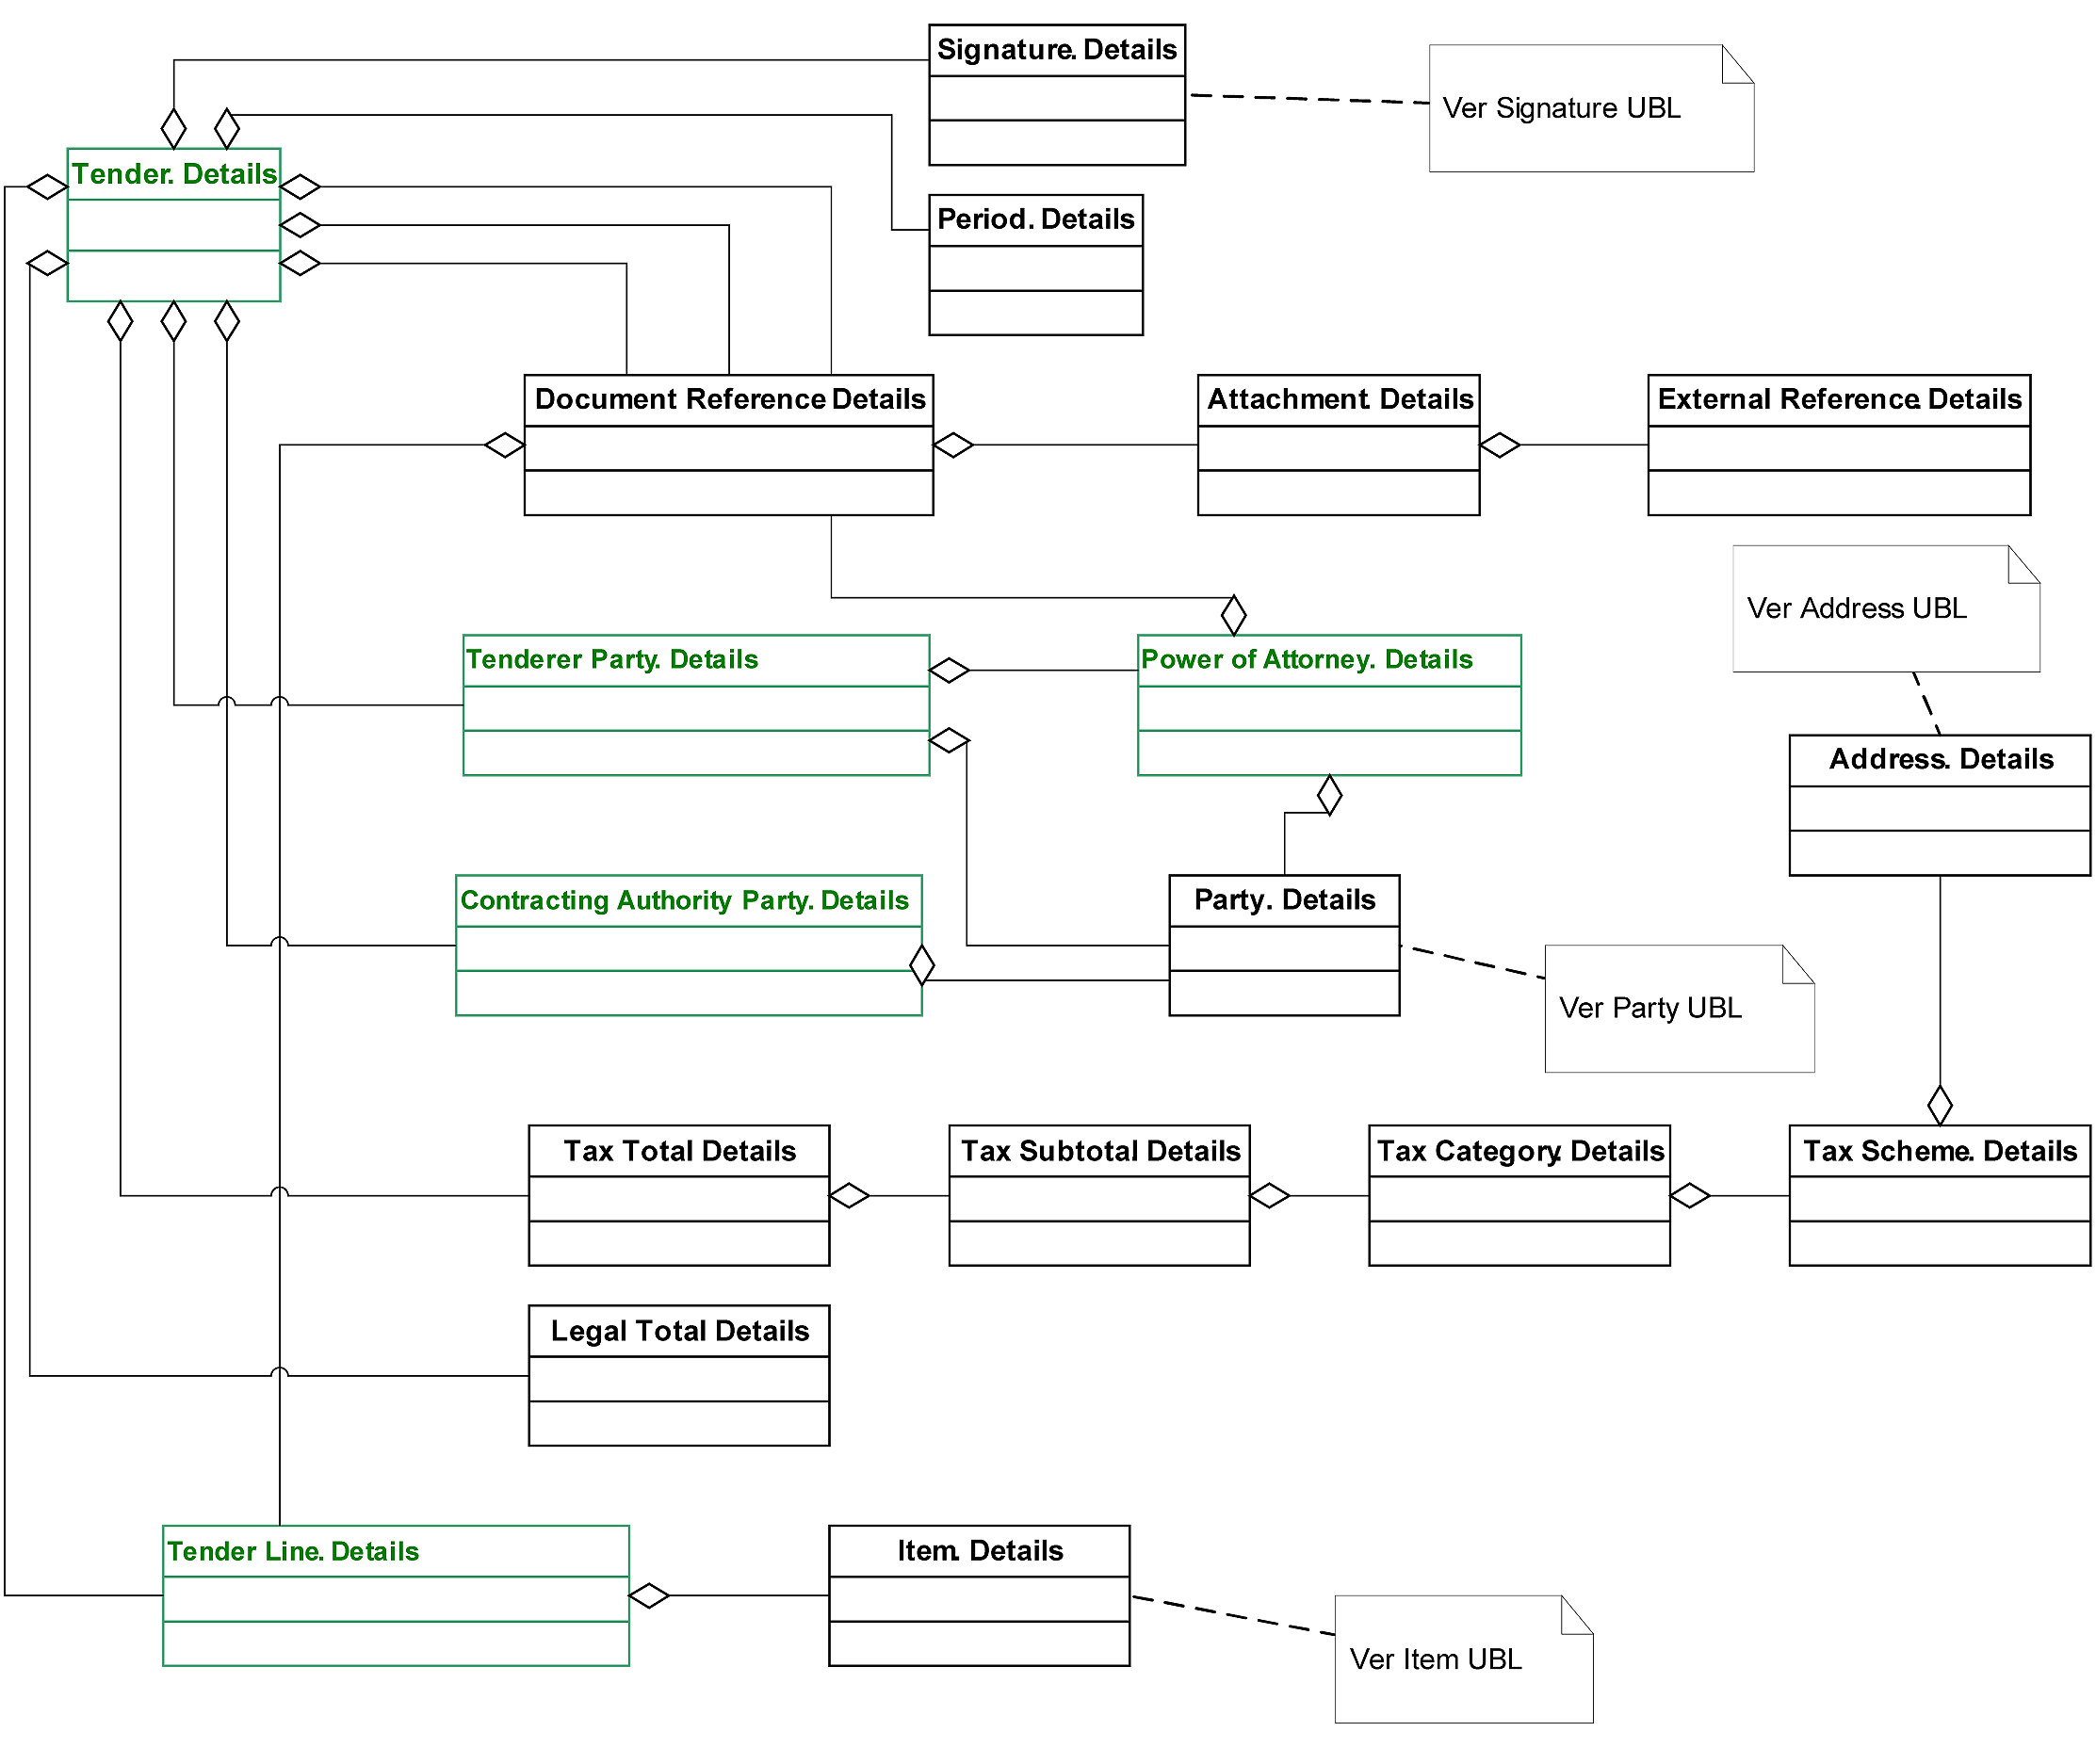
\includegraphics[width=16cm]{images/phd/eproc/codice-3-tender}
\caption{Modelo del Proceso de Contratación Pública Electrónica en CODICE v1.}
\label{fig:codice-3}
\end{figure}


\begin{figure}[!htb]
\centering
	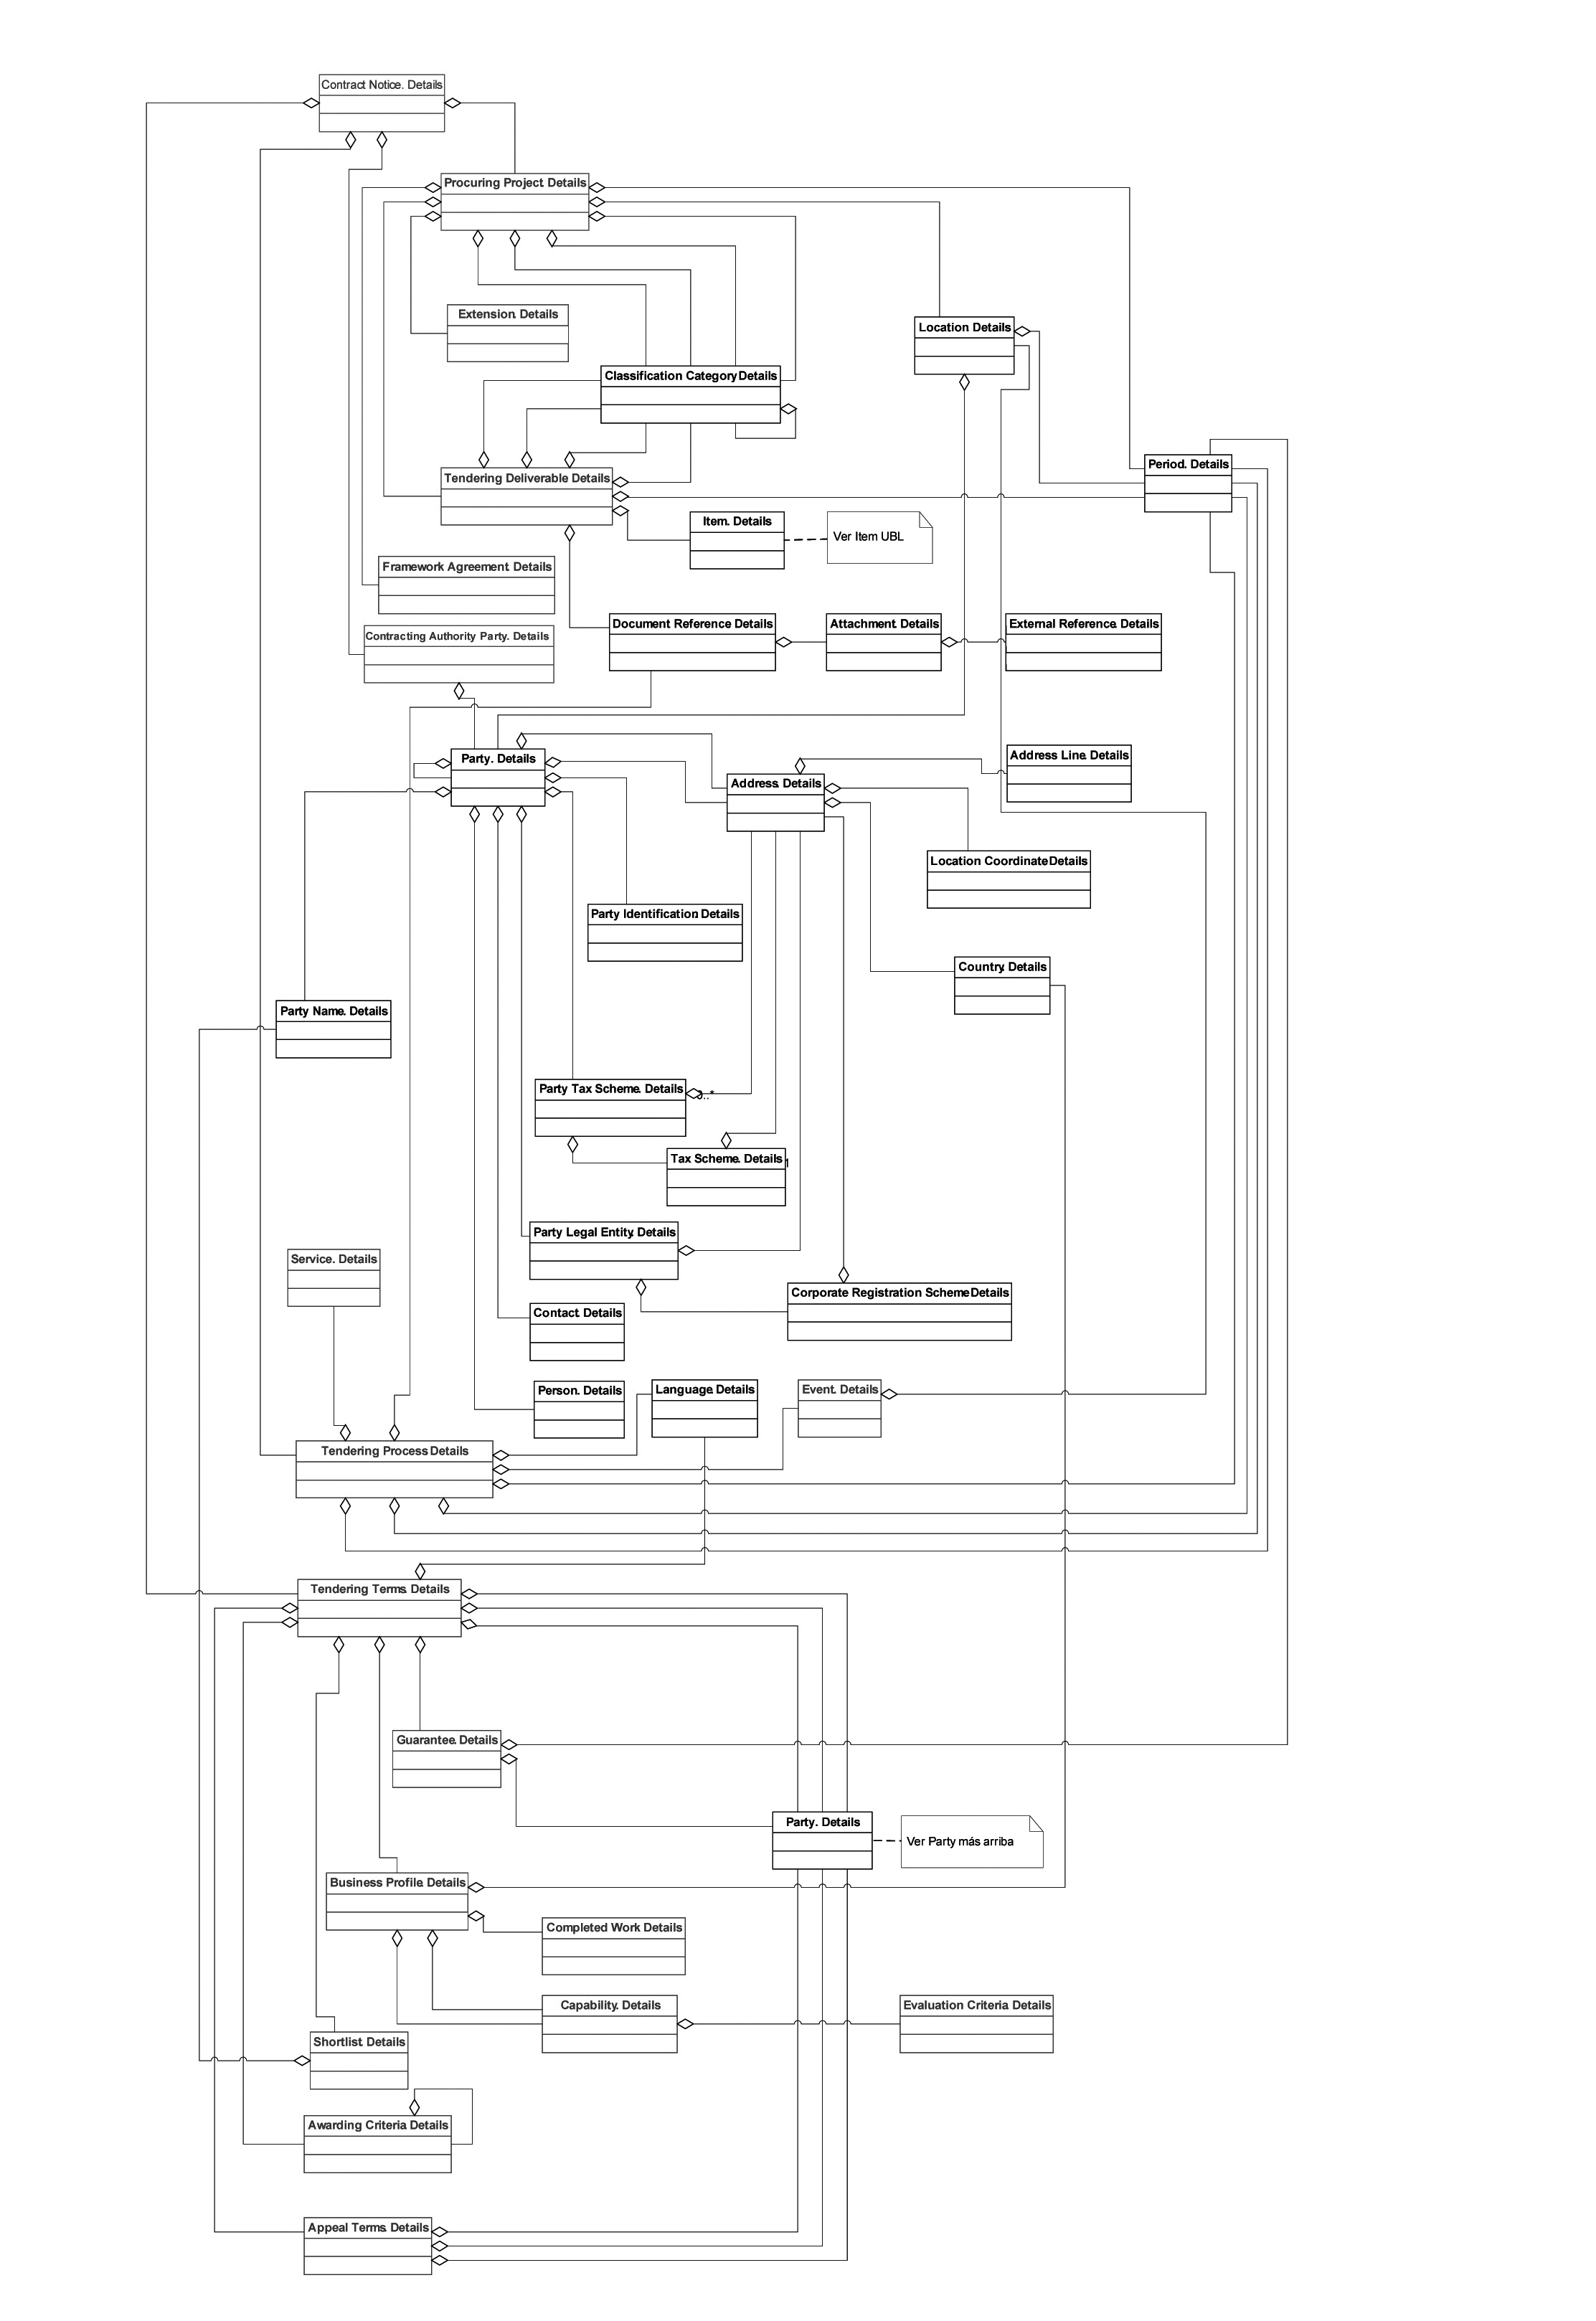
\includegraphics[width=14cm]{images/phd/eproc/codice-1}
\caption{Modelo de Información de Anuncio de Licitación en CODICE v1.}
\label{fig:codice-1}
\end{figure}

\begin{figure}[!htb]
\centering
	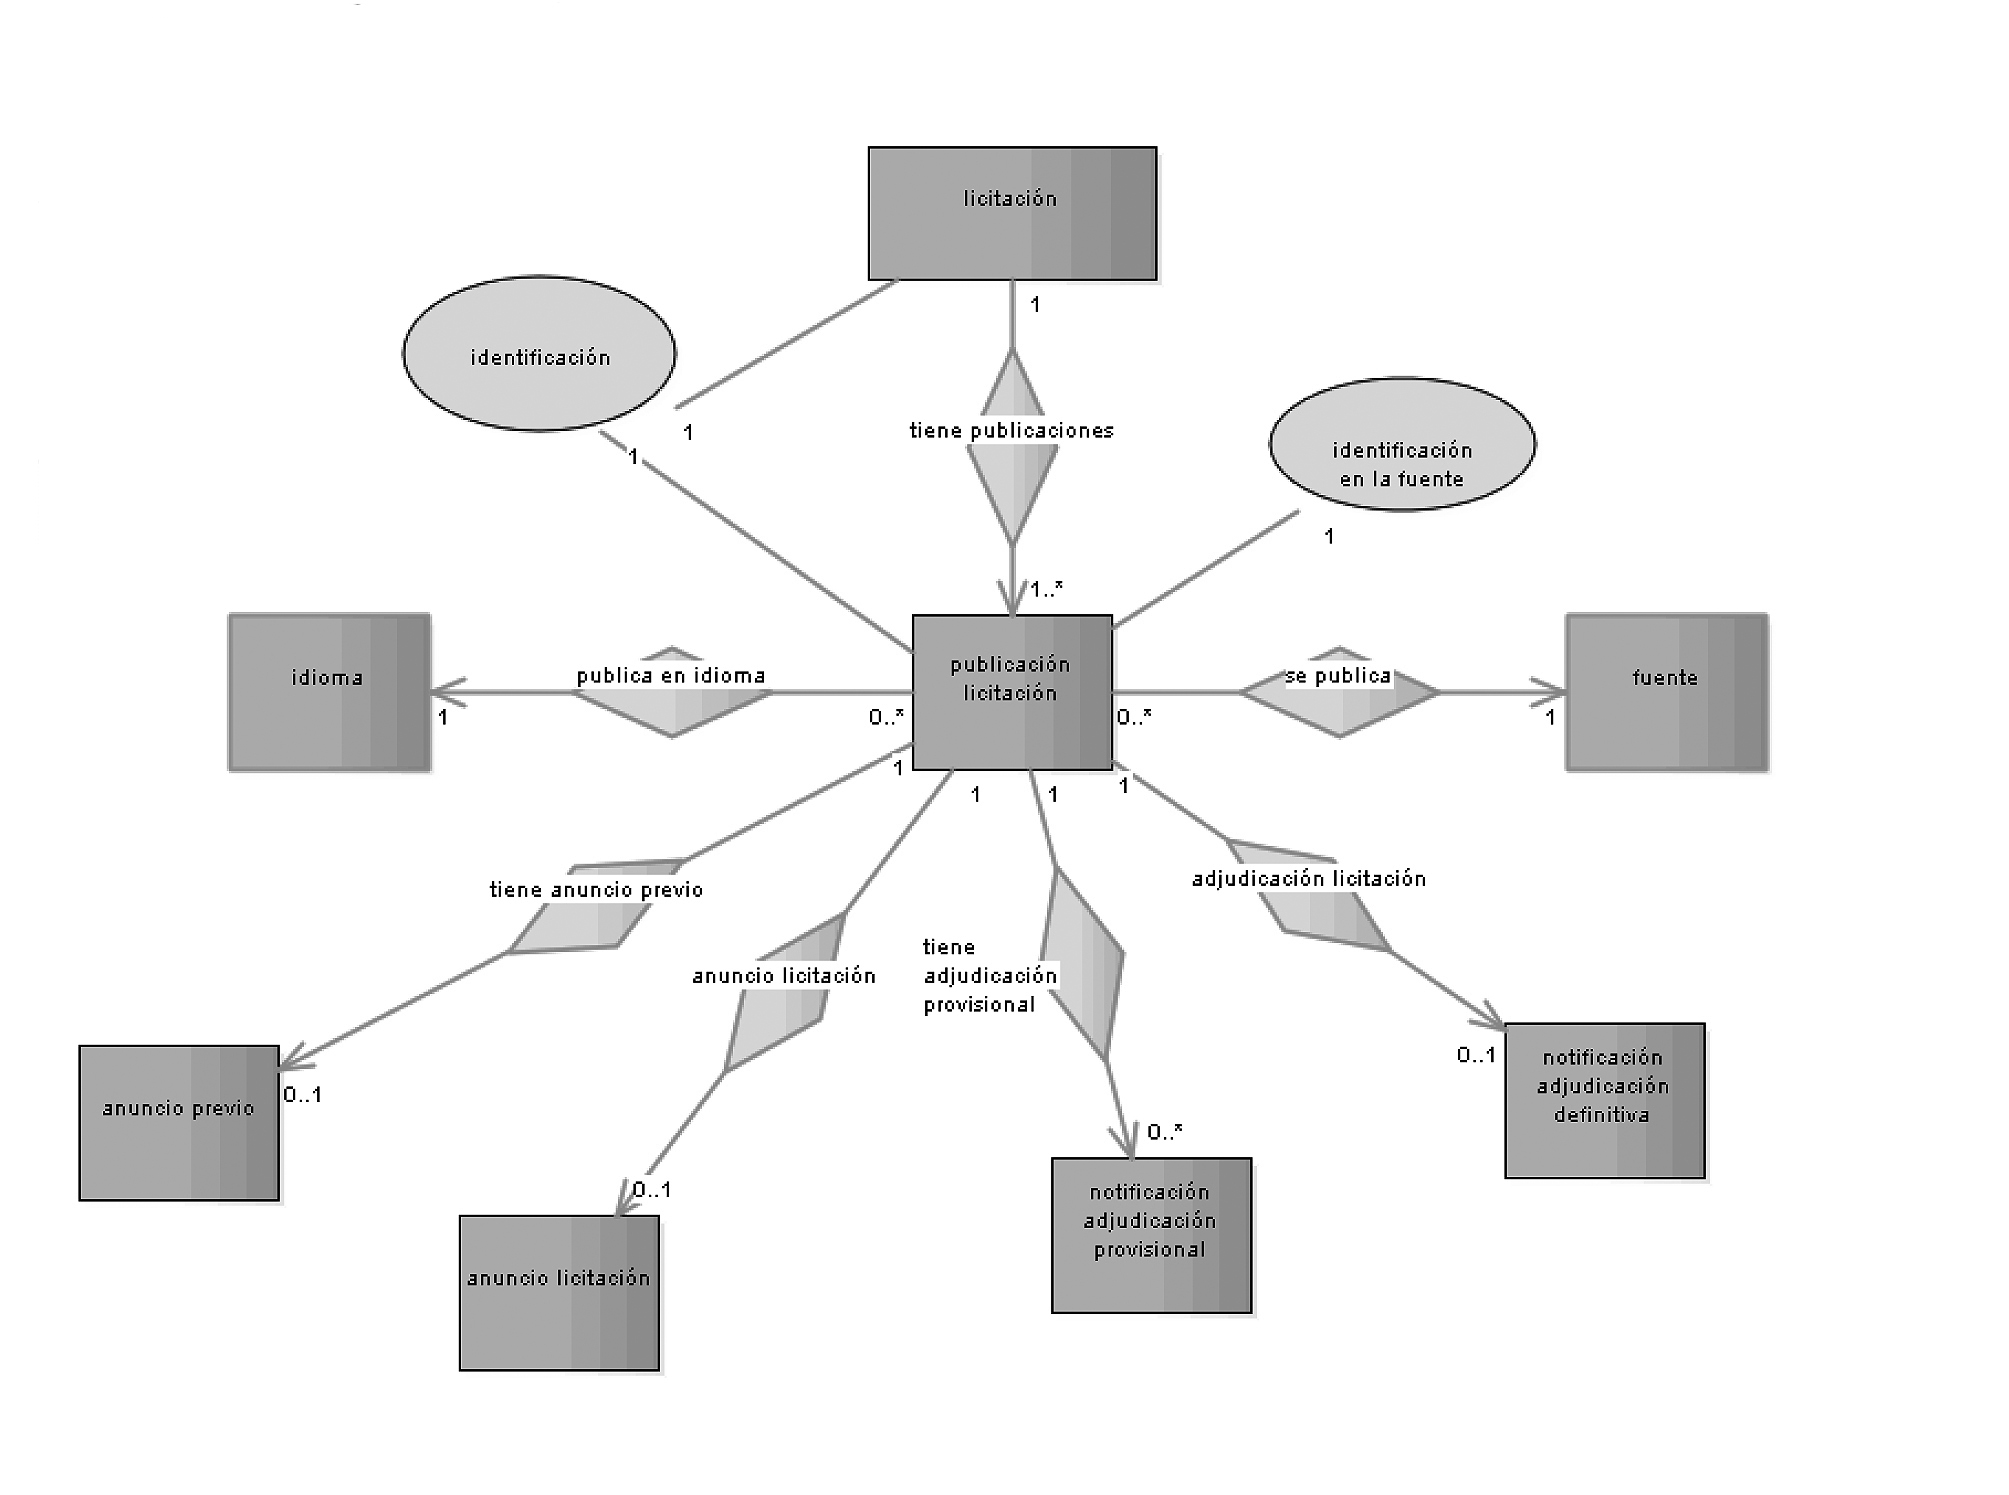
\includegraphics[width=18cm]{images/phd/eproc/10ders-1}
\caption{Modelo de Información de Anuncio de Licitación en \textit{opXML}.}
\label{fig:10ders-1}
\end{figure}

\clearpage
\section{Clasificaciones Estándar de Productos}\label{sect:pscs}
Los anuncios de licitación contienen información muy relevante para la búsqueda
de oportunidades de negocio para las distintas empresas, relativa a la localización,
la cuantía del contrato, la duración, etc., importante para concursar
en la adjudicación del contrato, sin embargo, la información clave en un anuncio
de licitación es el tipo de contrato que se va a adjudicar ya que con ello
se crea el mayor filtro posible para las posibles empresas. En este sentido,
han surgido muchas iniciativas~\cite{Leukel-findings} para aunar la adición de descriptores estándares~\cite{Leukel-standard}
a los anuncios de licitación. A este tipo de información se le denomina, de forma particular, esquemas o catálogos estándar de productos y 
servicios, en general se pueden asimilar a un sistema de organización de conocimiento como tesauros, taxonomías o sistemas de clasificación jerárquicos, utilizados
ampliamente para la organización~\cite{Leukel-automating} de grandes colecciones de información como 
documentos, textos, páginas web o recursos multimedia tanto en el ámbito público como privado~\cite{Leukel-comparative}. Estos vocabularios
permiten que los usuarios puedan anotar los objetos de información de una forma
sencilla para que posteriormente su consulta y acceso se simplifique. El uso
de estas técnicas de etiquetado con vocabularios controlados está ampliamente
asentado~\cite{Leukel-ecatalog2005} para describir el \textit{topic} de distintos objetos de información, 
suponiendo un primer paso para el tratamiento automático de la información.

\begin{figure}[!htb]
\centering
	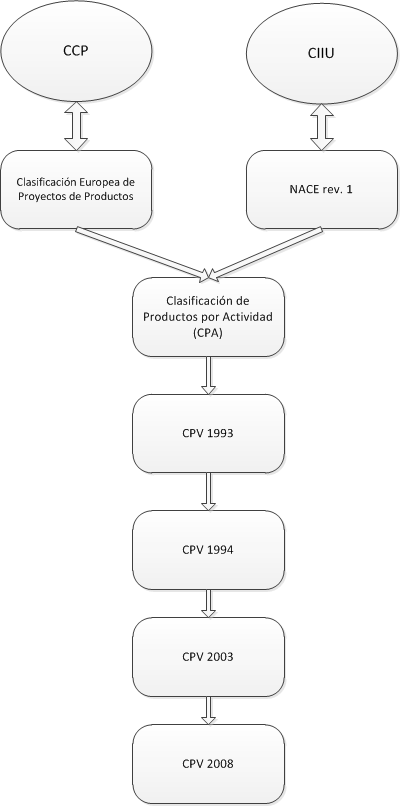
\includegraphics[width=6cm]{images/phd/eproc/evo-cpv}
\caption{Evolución \textit{Common Procurement Vocabulary}.}
\label{fig:evo-cpv}
\end{figure}

Por ejemplo en el contexto europeo han surgido muchas clasificaciones de este tipo
para distintos dominios, disponibles en el servidor de metadatos \gls{RAMON}.
Entre ellos se puede destacar ``\textit{the European Schedule of Occupational Diseases}'' en el 
campo de la salud, ``\textit{the European Education Thesaurus or the European Glossary on Education}''
en materia de educación, ``\textit{the International Standard Classification of Occupations}'' en el ámbito trabajo, etc.
La estructura de estos sistemas de clasificación es similar: jerarquía de entidades y multiling\"{u}ismo, contienen sin embargo, 
factores heterogéneos que impiden su interoperabilidad y que deben ser abordados para conseguir un aprovechamiento eficiente del esfuerzo que supone realizar este tipo
de clasificaciones.

En el campo de la contratación pública electrónica es evidente que este tipo
de paradigmas de clasificación controlada de documentación como anuncios de licitación, lotes,
contratos, etc., es clave para realizar una gestión eficiente de la gran cantidad de información
y documentos que son generados constantemente. Como consecuencia, una de las primeras medidas
impulsadas desde la Comisión Europea ha sido la realización del ``\textit{Common Procurement Vocabulary}'' (\gls{CPV})~\cite{cpvguide}, se trata de 
una clasificación para describir los objetos de un contrato permitiendo a los agentes
implicados una forma sencilla de buscar los anuncios de licitación. De esta forma, se ha
conseguido armonizar el sistema de codificación de los objetos de contrato. Además, el uso
del CPV es obligatorio desde el 1 de febrero de 2006 según se establece en la Directiva 
Regulation (EC) No 2195/2002~\cite{r2195} del Parlamento Europeo. En el ámbito europeo el CPV es, sin duda, 
el vocabulario controlado clave en la esfera de la contratación pública electrónica, que
ha sido fruto del esfuerzo y trabajo desde otras clasificaciones, ver Figura~\ref{fig:evo-cpv}, como la ``Clasificación
Central de Productos'' (\gls{CPC}), la ``Clasificación Industrial Internacional Uniforme'' (\gls{CIIU})
y la ``Clasificación de Productos por Actividades'' (\gls{CPA})

\begin{longtable}[c]{|p{6cm}|l|p{6cm}|} 
\hline
  \textbf{Clasificación} &  \textbf{Acrónimo} & \textbf{Organismo} \\\hline
\endhead
\textit{Combined Nomenclature} 2012 (desde 1995) & \gls{CN} & Unión Europea  \\ \hline
\textit{Central Product Classification}, version 2 (2008) & \gls{CPC} & Unión Europea \\ \hline
Clasificación de Productos por Actividad (2008) & \gls{CPA} & Unión Europea \\ \hline
\textit{Integrated Tariff of the European Communities)} & \gls{TARIC} & Unión Europea\\ \hline
\textit{International Standard Industrial Classification of All Economic Activities, Rev.4} & \gls{ISIC} & \textit{United Nations Statistics Division} \\ \hline
\textit{North American Product Classification System} & \gls{NAPCS} & Agencias estadísticas de Canadá, México y Estados Unidos\\ \hline
\textit{North American Industry Classification System} 2007 y 2012 & \gls{NAICS} & Gobierno de Estados Unidos \\ \hline
\textit{PRODuction COMmunautaire} & \gls{PRODCOM} & Unión Europea \\ \hline
\textit{Standard International Trade Classification, Revision 4} & \gls{SITC} & \textit{United Nations Statistics Division} \\ \hline
\textit{Nomenclature générale des activités économiques dans les Communautés européennes} & \gls{NACE} & Unión Europea \\ \hline
\textit{United Nations Standard Products and Services Code} & \gls{UNSPSC} & Consorcio entre ellos la ONU\\ \hline
  \multicolumn{3}{|c|}{\ldots}  \\ \hline
\hline
\caption{Catálogo de Clasificaciones Estándar de Productos.}\label{table:pscs}\\    
\end{longtable}

Además del CPV existen otras muchas clasificaciones~\cite{Norbert-class} interesantes, ver Tabla~\ref{table:pscs}, en comercio electrónico o bien
para la extracción de estadísticas, que han sido formuladas por diferentes organismos como
la \gls{UNESCO}, \gls{ONU} o el Gobierno de Estados Unidos, que actualmente tienen en el mejor de los casos \textit{mapeos} entre ellas, 
pero cuyo acceso suele ser complicado tanto por los formatos en los que se presentan, habitualmente MSExcel o \gls{PDF}, como por 
las aplicaciones y sistemas de búsqueda muy rígidos. 

El uso de estas clasificaciones es clave para la trazabilidad de proveedores de productos y servicios,
sistemas de anotación y etiquetado, extracción de información, etc. En el contexto de los anuncios
de licitación representan el método de especificar el objeto del contrato pero no todo
son ventajas, ya que al existir una amplia variedad, es difícil mantener la consistencia entre ellas
y sus distintas versiones, forzando a que se dupliquen esfuerzos en los distintos organismos para 
extraer información basada en estos códigos. 



\section{Información sobre Organizaciones}
\textit{An organization is considered to be a set of constraints on the activities performed by agents}. 

Este enfoque de organización fue presentando por Max Weber~\cite{Weber1978}, posteriormente Mintzberg realizó un análisis
de las estructuras organizacionales distinguiendo entre cinco tipos y configuraciones diferentes. Estos enfoques
ponen de manifiesto los mecanismos que operan dentro de las organizaciones con el objetivo
de coordinarse para conseguir un determinado objetivo materializado a través de diferentes metas,
procesos y reglas de negocio, posición en el mercado y comunicación. Existen trabajos~\cite{Fox95anorganisation}
en los cuales se intenta modelar la estructura de una organización, pero que no ha abordado problemas como:
1) falta de información para definir el \textit{status} de una organización, 2) maraña de subdivisiones
para especificar la estructura entre los elementos de la organización, 3) ausencia de capacidades léxicas
para describir los conceptos y relaciones que se manejan en una organización, 4) distintos tipos
de nombrado, etc. 

La problemática para definir la estructura de una organización y su actividad no es sencilla, ya que puede
ser muy diversa dependiendo de su organización, objetivos particulares, etc., es por ello que en el campo
de la contratación pública electrónica resulta de gran valor la posibilidad de disponer de la información
de los agentes implicados en el proceso administrativo, para así poder trazar su actividad a lo largo
del tiempo. Desde un punto de vista del órgano contratante, su perfil debe estar disponible al público, el cual, 
además de los anuncios de licitación debe comprender la información de contacto, persona encargada, etc., 
toda esta información actualmente está accesible pero de una forma ligeramente rudimentaria. De igual forma, cuando
los contratos son adjudicados, se dispone de la información relativa a la empresa adjudicataria pero de nuevo
el acceso a esta información sigue un modelo tradicional. Un proceso lógico sería que una entidad especificara
su perfil de contrante siguiendo un estándar en cuanto a su organización interna y que por otro lado
las empresas pudieran definir un perfil en el cual indicar sus intereses y así facilitar el proceso de 
encaje entre tipos de contrato e intereses. 

\section{Evaluación del estado actual del mundo de\\ \textit{e-Procurement}}
En este capítulo se han repasado los conceptos clave sobre contratación
pública y en concreto la contratación pública electrónica. Desde la
Unión Europea existe un claro compromiso y liderazgo por impulsar este proceso
administrativo por la relevancia y el impacto que tiene en la sociedad, ya que sin lugar a dudas las cifras de inversión y gasto que se manejan
resultan de gran interés para las empresas de todo tipo y sector. Sin embargo, aunque las distintas iniciativas han conseguido avanzar en la 
consecución de este gran reto, existen puntos clave en los cuales las soluciones existentes no han
conseguido desarrollar toda su capacidad para atraer a las empresas
y así conseguir un mercado competitivo a nivel paneuropeo. En este sentido,
la disponibilidad de soluciones técnicas ya existentes así como las que
se están desarrollando y la transferencia tecnológica desde los entornos
académicos deben mejorar las fases de \eproc. Esta inversión
en nuevas capacidades es clave para la adopción y uso efectivo de este proceso administrativo
de forma electrónica. Por ello, son esenciales tanto la publicación como la accesibilidad transfronteriza
a la información y sistemas de contratación pública electrónica. 

Los retos que se plantean son diversos y abarcan desde la generación de confianza suficiente
entre entidades adjudicadoras y proveedores a través de un marco legislativo adecuado, hasta
la generación de herramientas y medios que permitan la comunicación efectiva entre los distintos
agentes participantes en el proceso. Muchas veces, los requisitos técnicos en lugar de facilitar
la adopción de una nueva metodología de trabajo, suponen una gran barrera de entrada, un simple sistema de autenticación se puede
convertir en un gran inconveniente para el uso de los medios electrónicos. No obstante,
la transición hacia este nuevo mundo electrónico para la contratación se está realizando
de forma sostenible y a distintas velocidades, dependiendo de las capacidades de las propias
Administraciones. Las prioridades para realizar el despliegue definitivo se centran en el uso
de medidas que actúan como incentivo o penalización para acelerar este nuevo método, impulsar
la participación paneuropea en los distintos procesos de licitación pública, simplificando 
las condiciones a satisfacer para el uso de los nuevos sistemas y facilitando la autenticación
entre los distintos agentes económicos. Finalmente, todos estos retos y prioridades se realizarán
bajo una base normalizada, tanto en tecnología como en estándares, para la distinta documentación
generada durante el proceso con el objetivo final de que paulatinamente todo tipo de empresas
puedan competir por los contratos públicos bajo las mismas condiciones con las consiguientes
ventajas para el mercado económico común.

\section{Modelos Conceptuales de Dominio}\label{sect:mcds}
% 


\begin{figure}[!htb]
\centering
	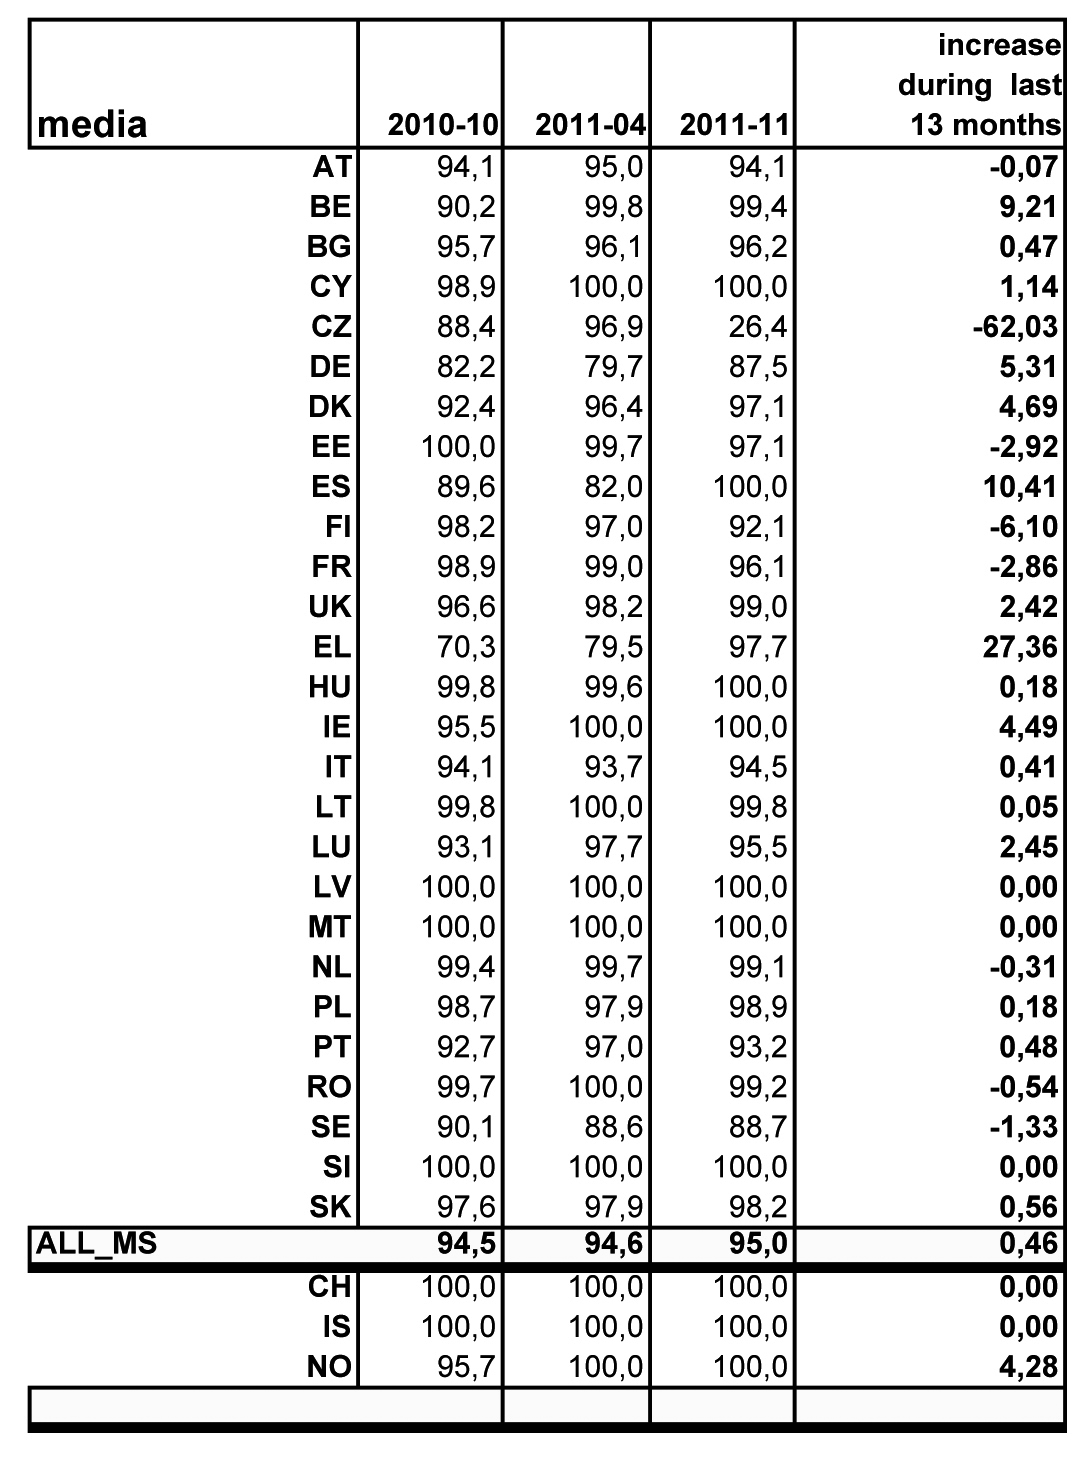
\includegraphics[width=10cm]{images/phd/eproc/circa-2}
\caption{Porcentaje y Tipo de Publicación de Anuncios de Licitación en TED (2).}
\label{fig:circa-1}
\end{figure}



\begin{figure}[!htb]
\centering
	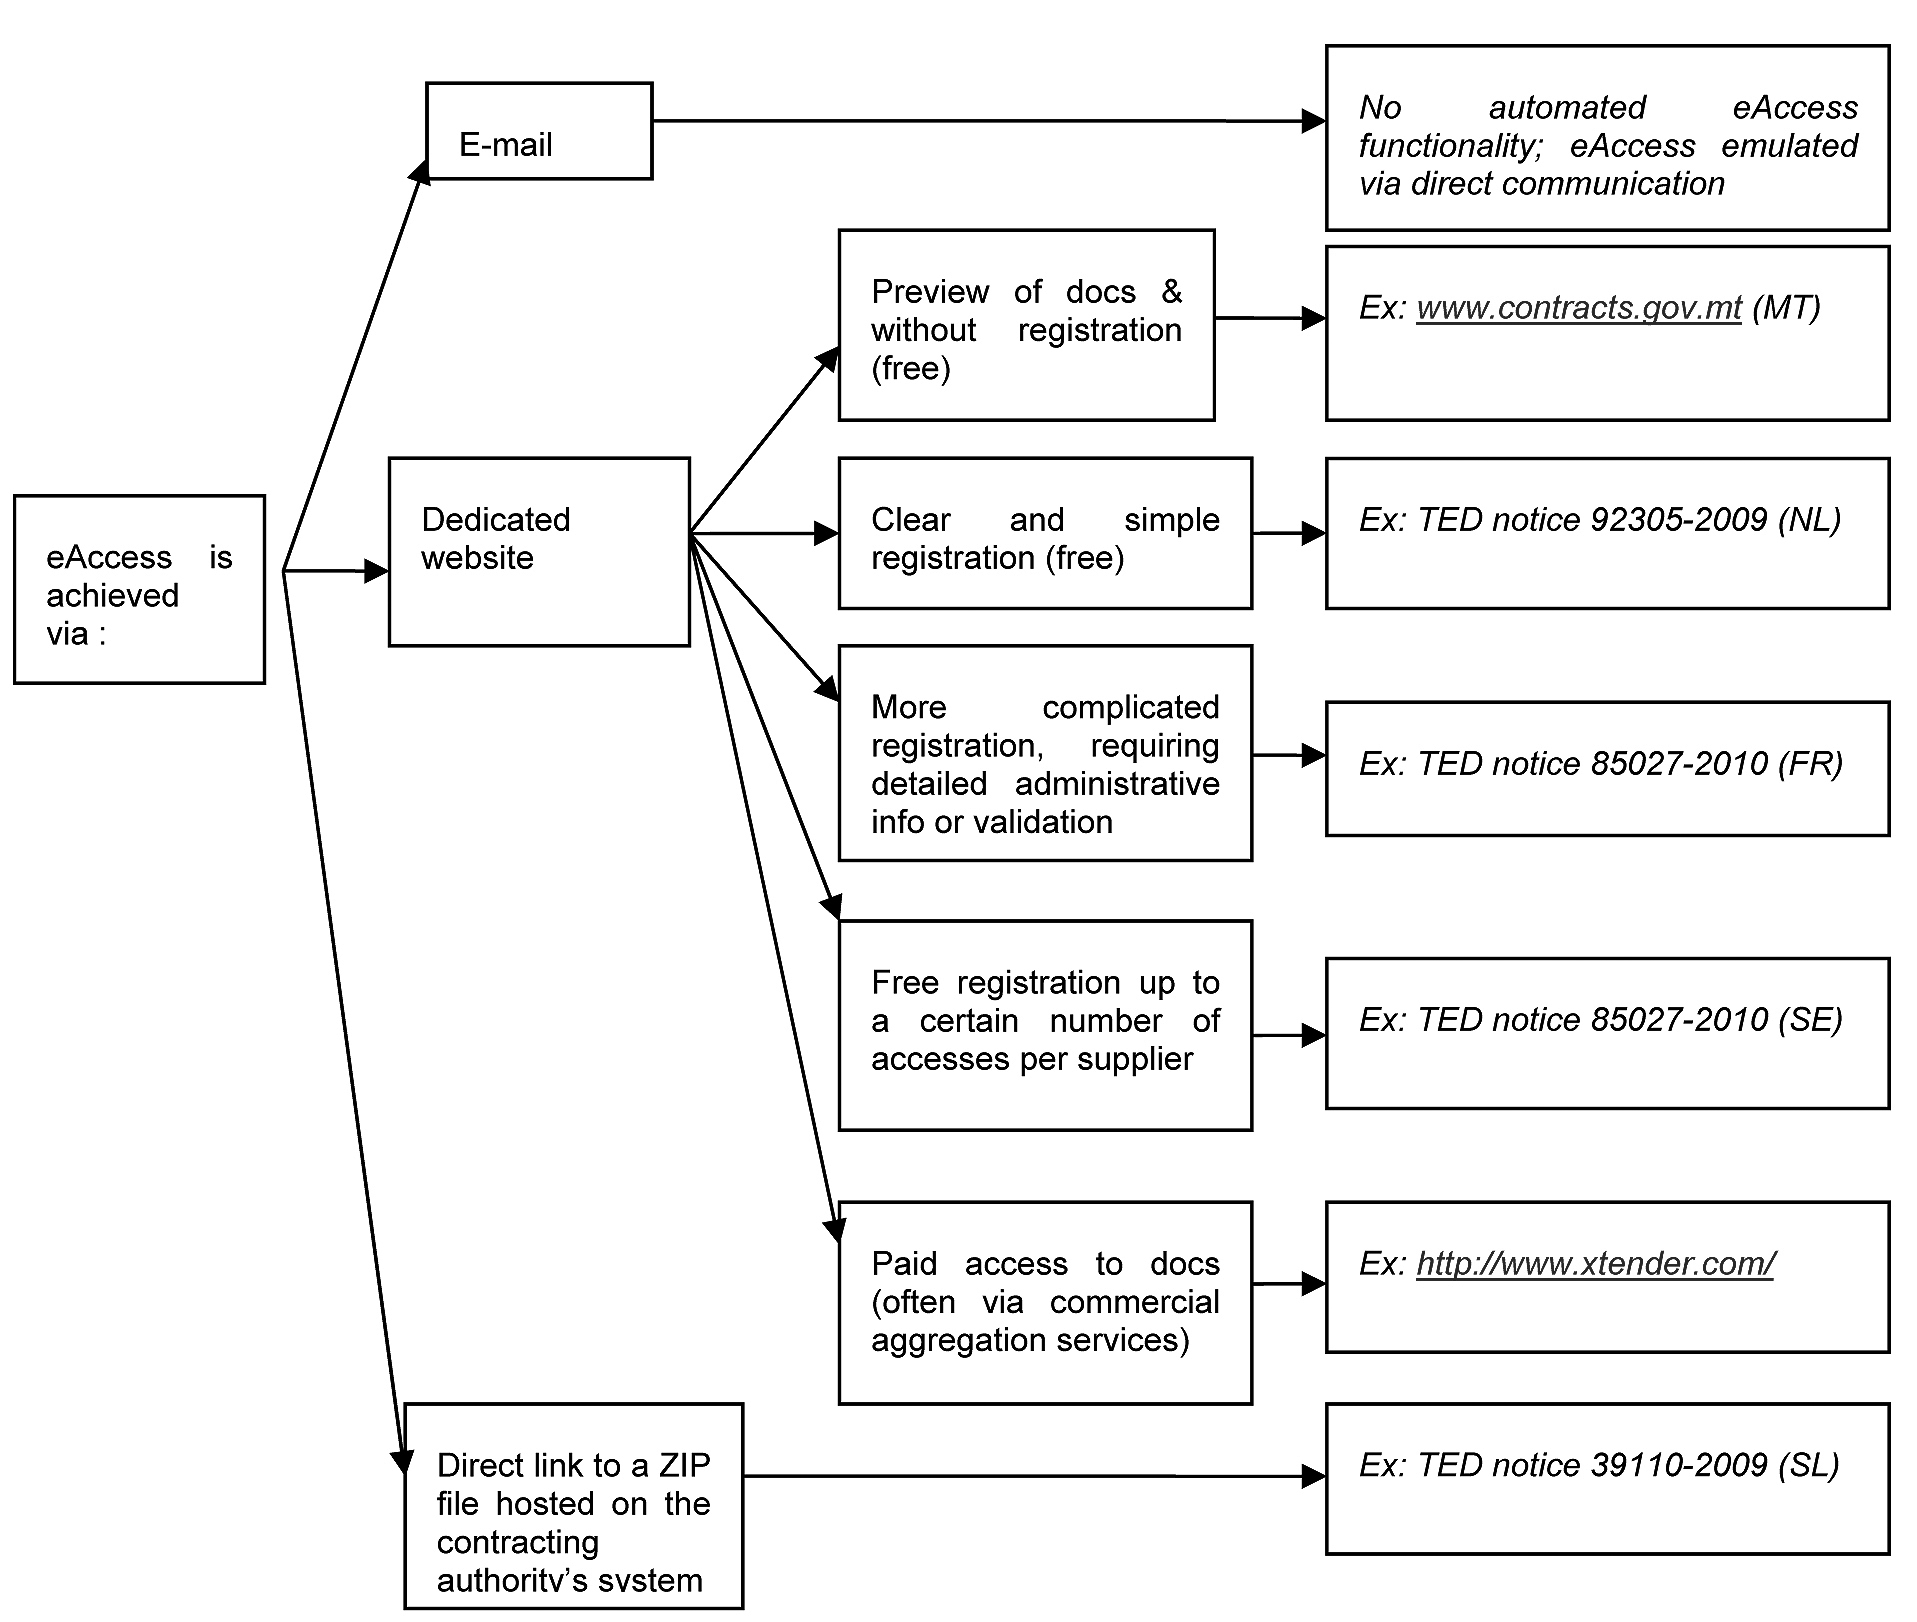
\includegraphics[width=10cm]{images/phd/eproc/ted-4}
\caption{Características en \textit{eAccess} de la Unión Europea por Siemens.}
\label{fig:ted-4}
\end{figure}



\begin{figure}[!htb]
\centering
	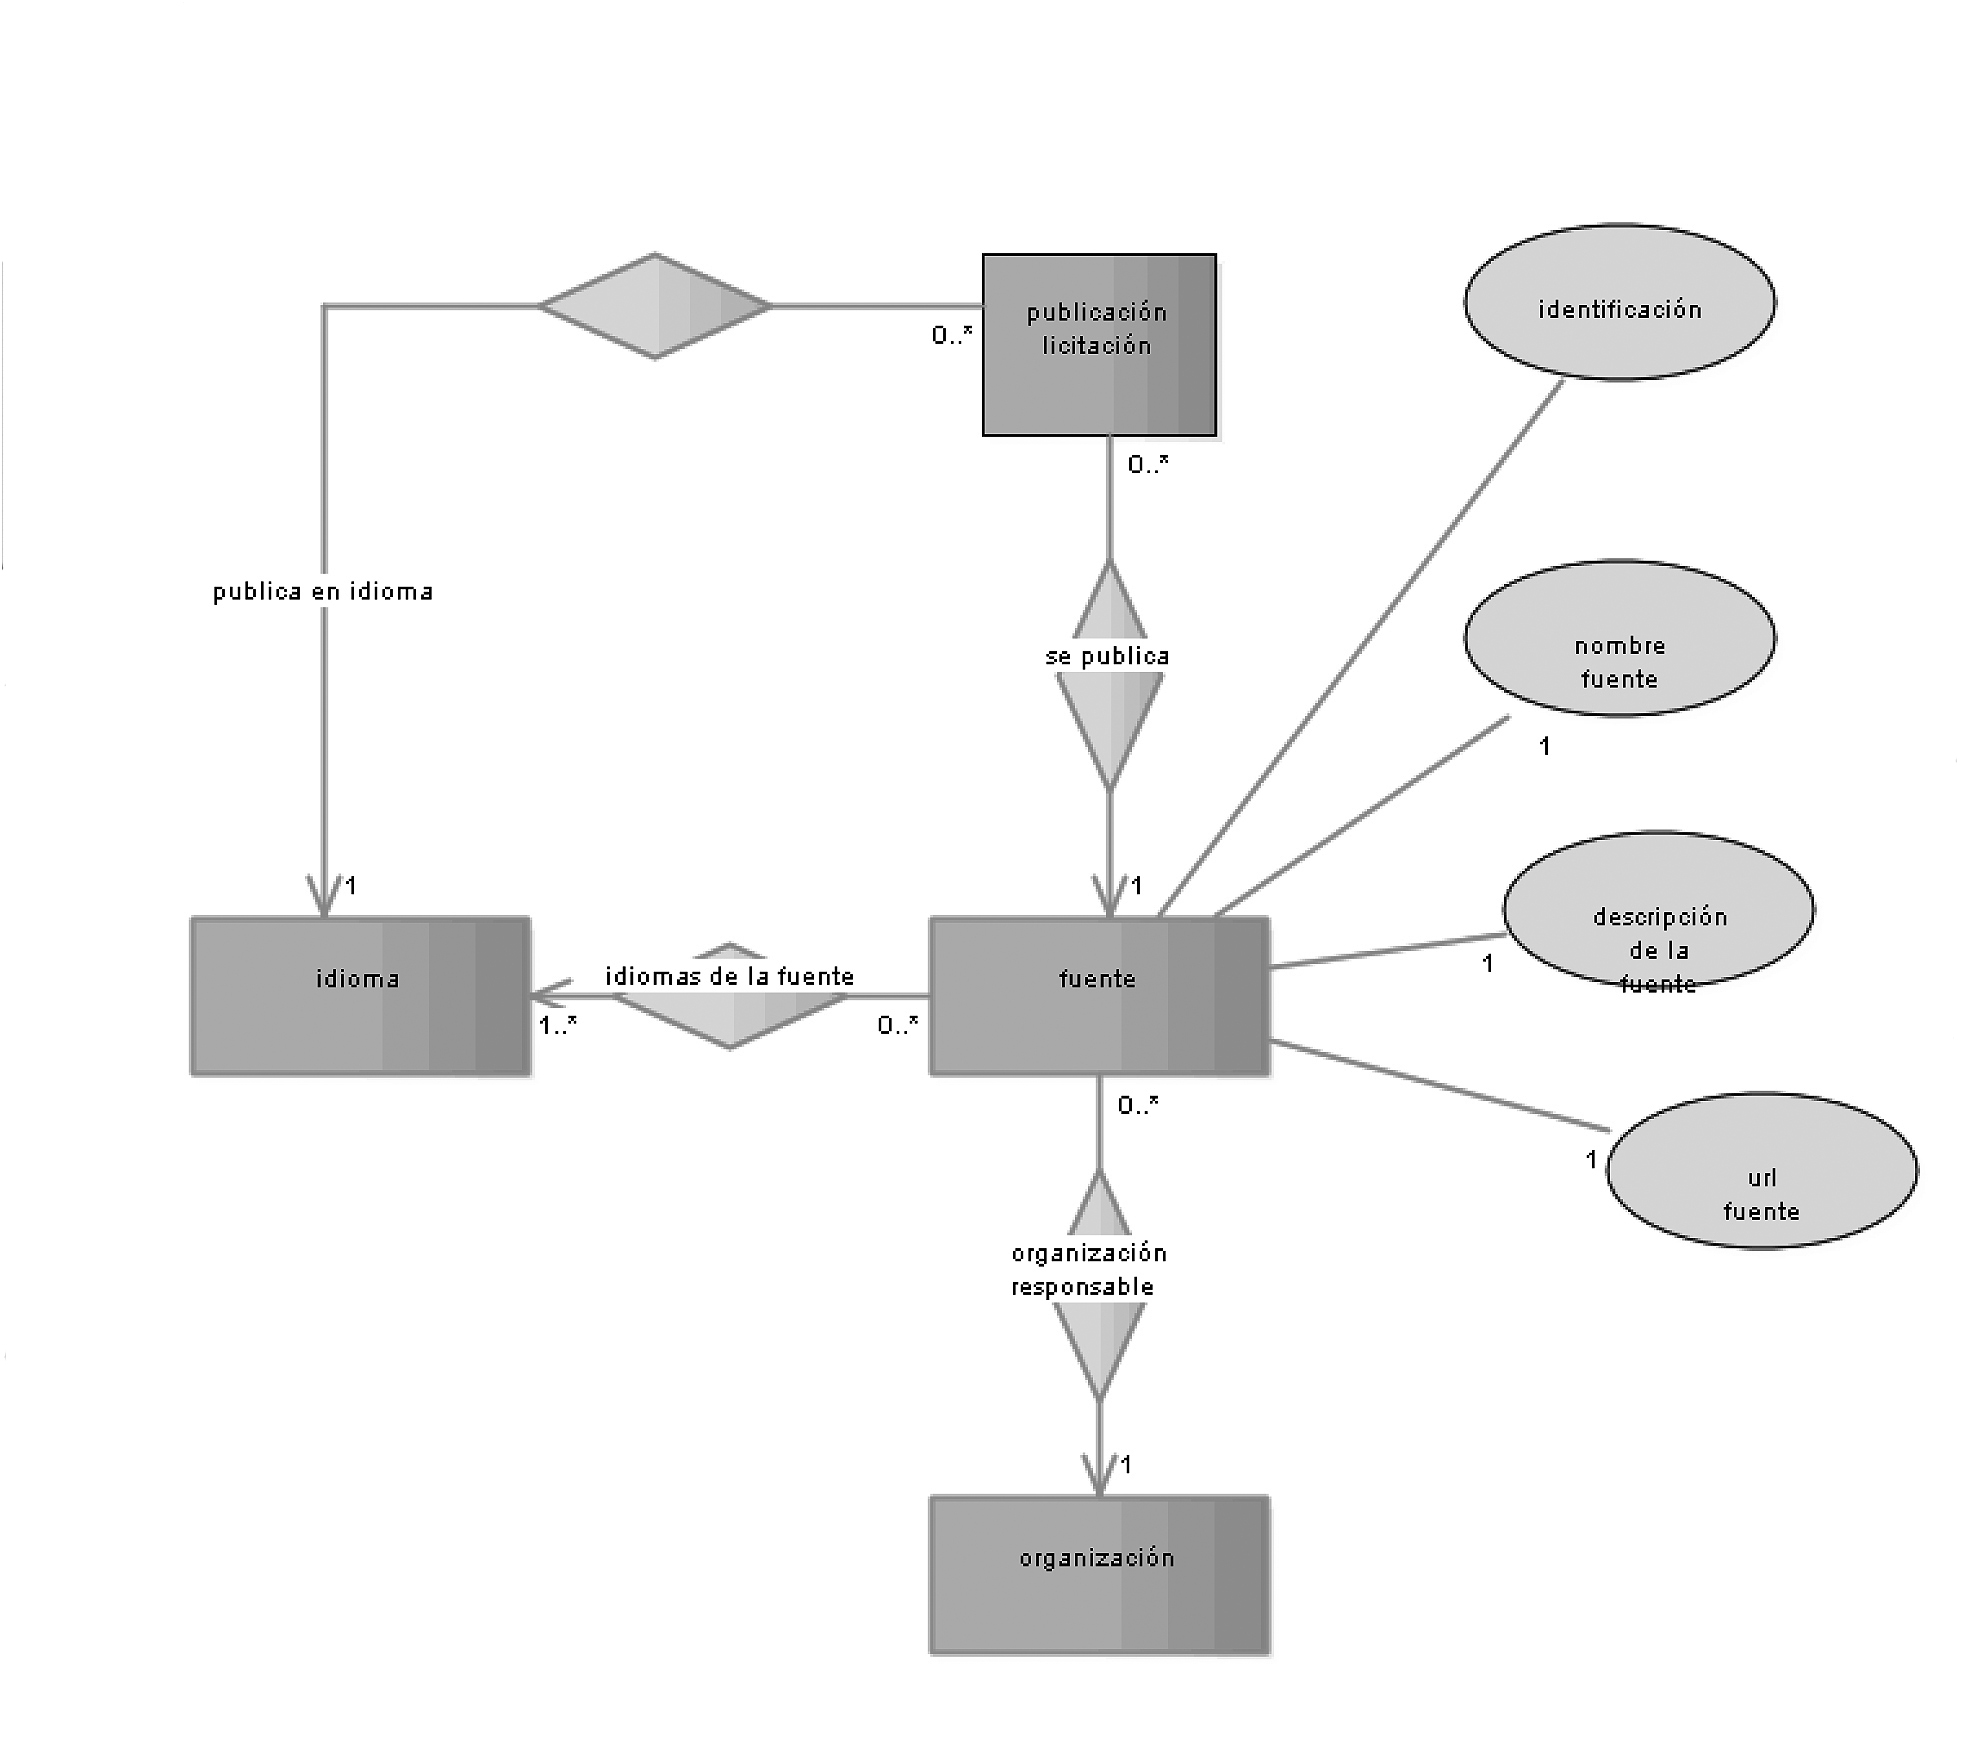
\includegraphics[width=10cm]{images/phd/eproc/10ders-8}
\caption{Fuente de Publicación en el proyecto 10ders.}
\label{fig:10ders-8}
\end{figure}

\begin{figure}[!htb]
\centering
	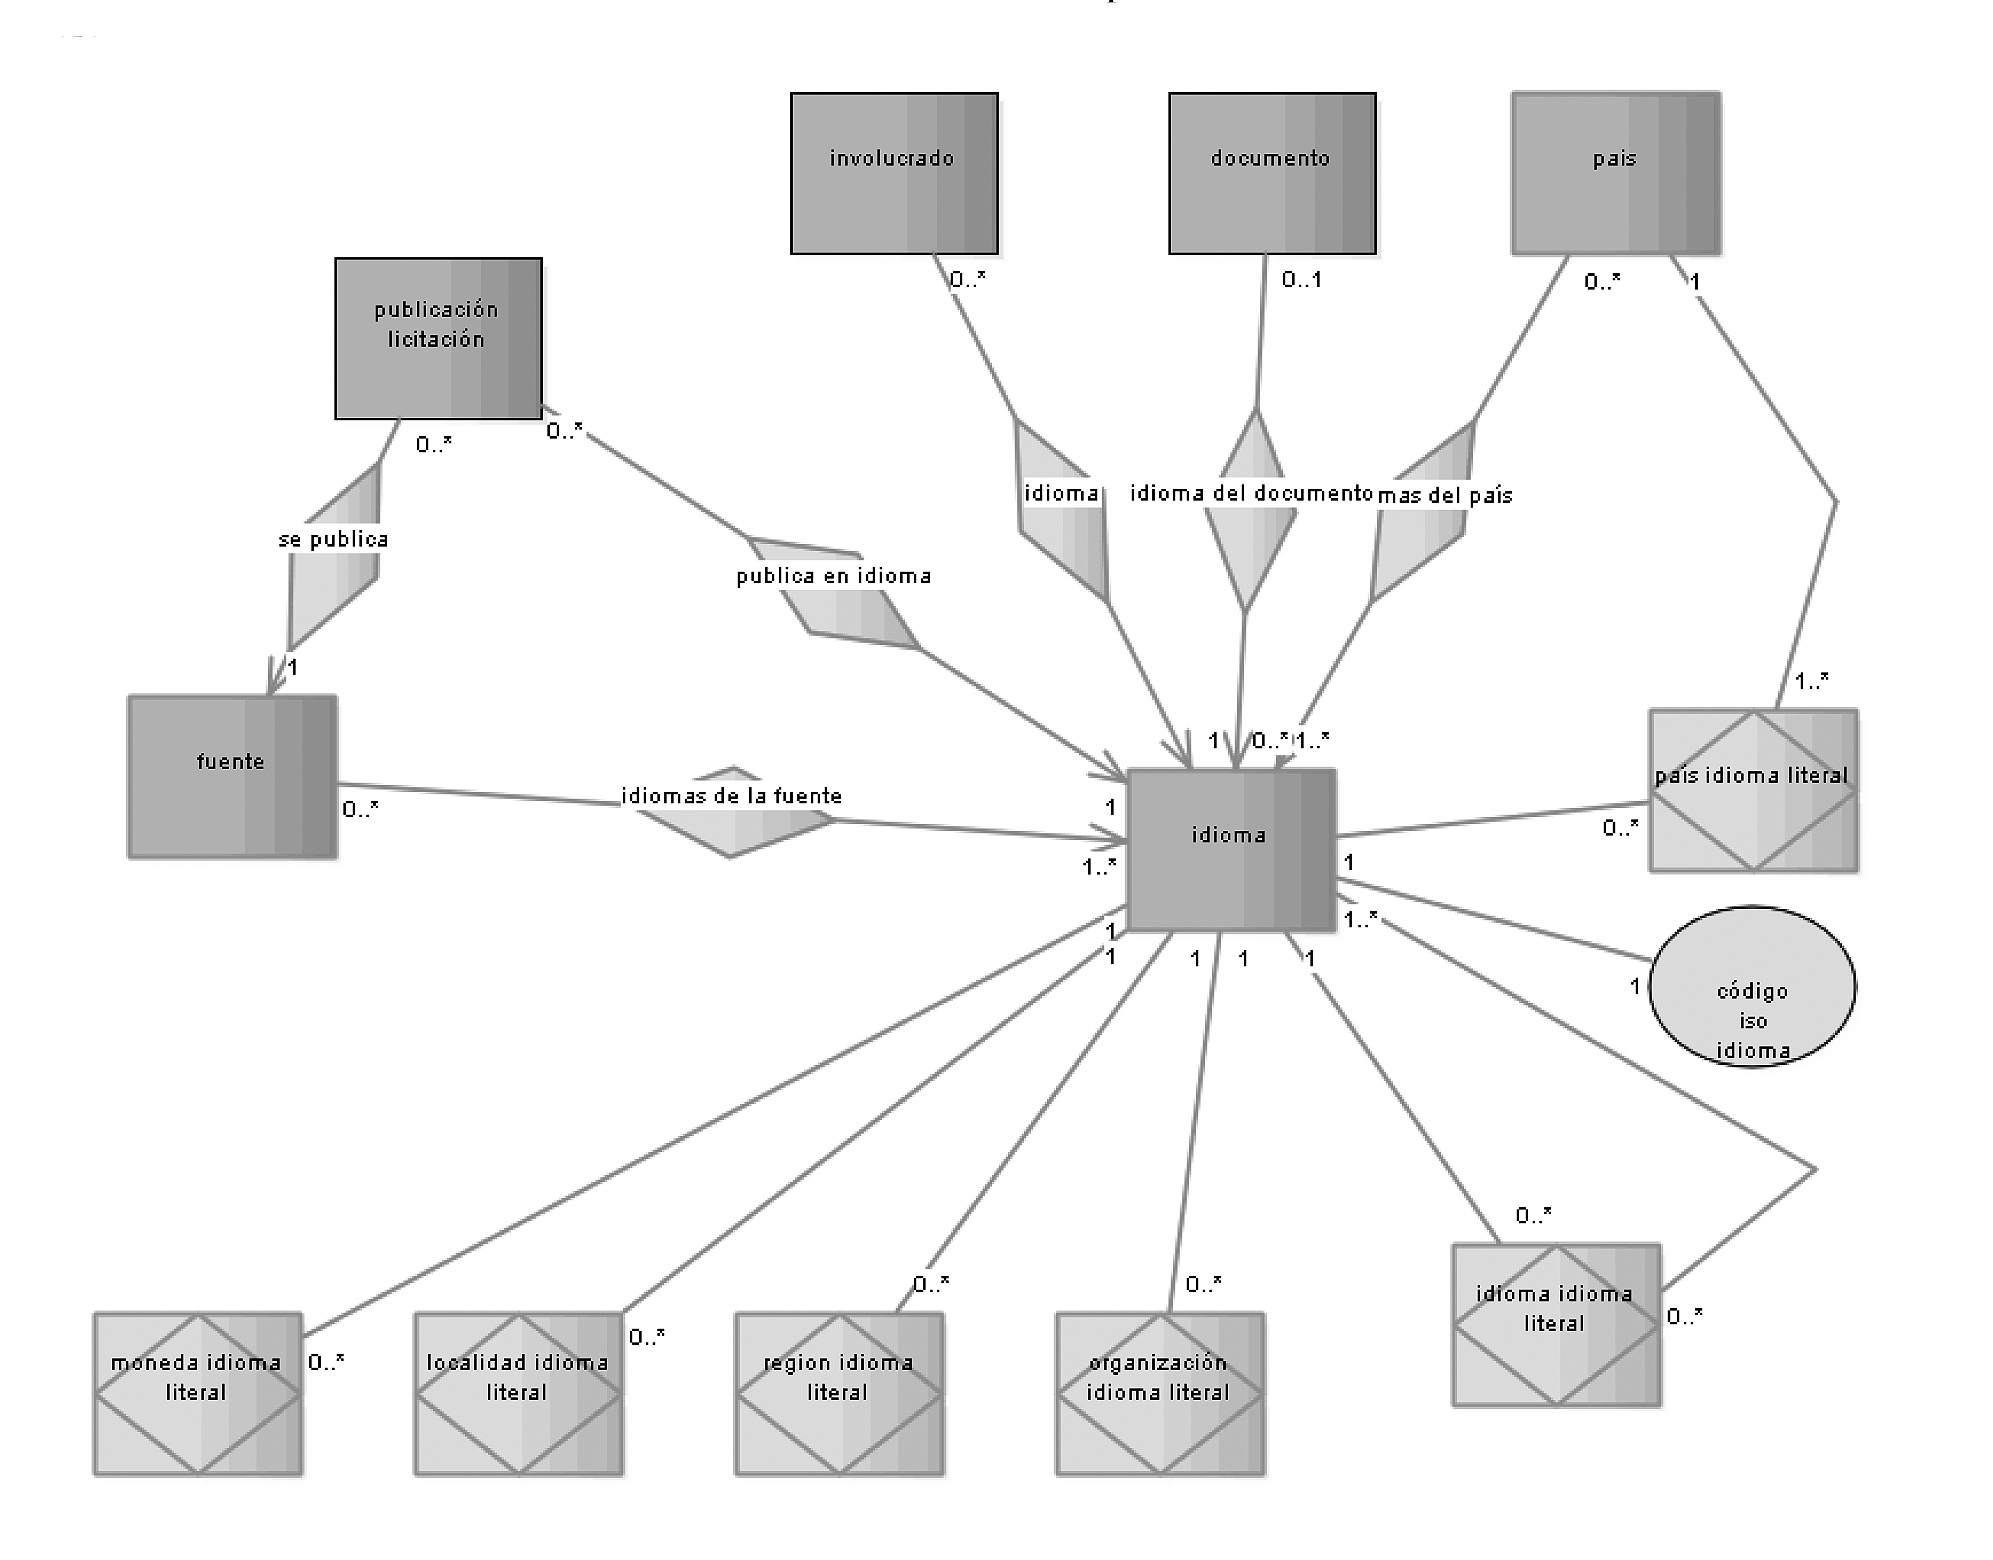
\includegraphics[width=10cm]{images/phd/eproc/10ders-9}
\caption{Idioma en el proyecto 10ders.}
\label{fig:10ders-9}
\end{figure}



\begin{figure}[!htb]
\centering
	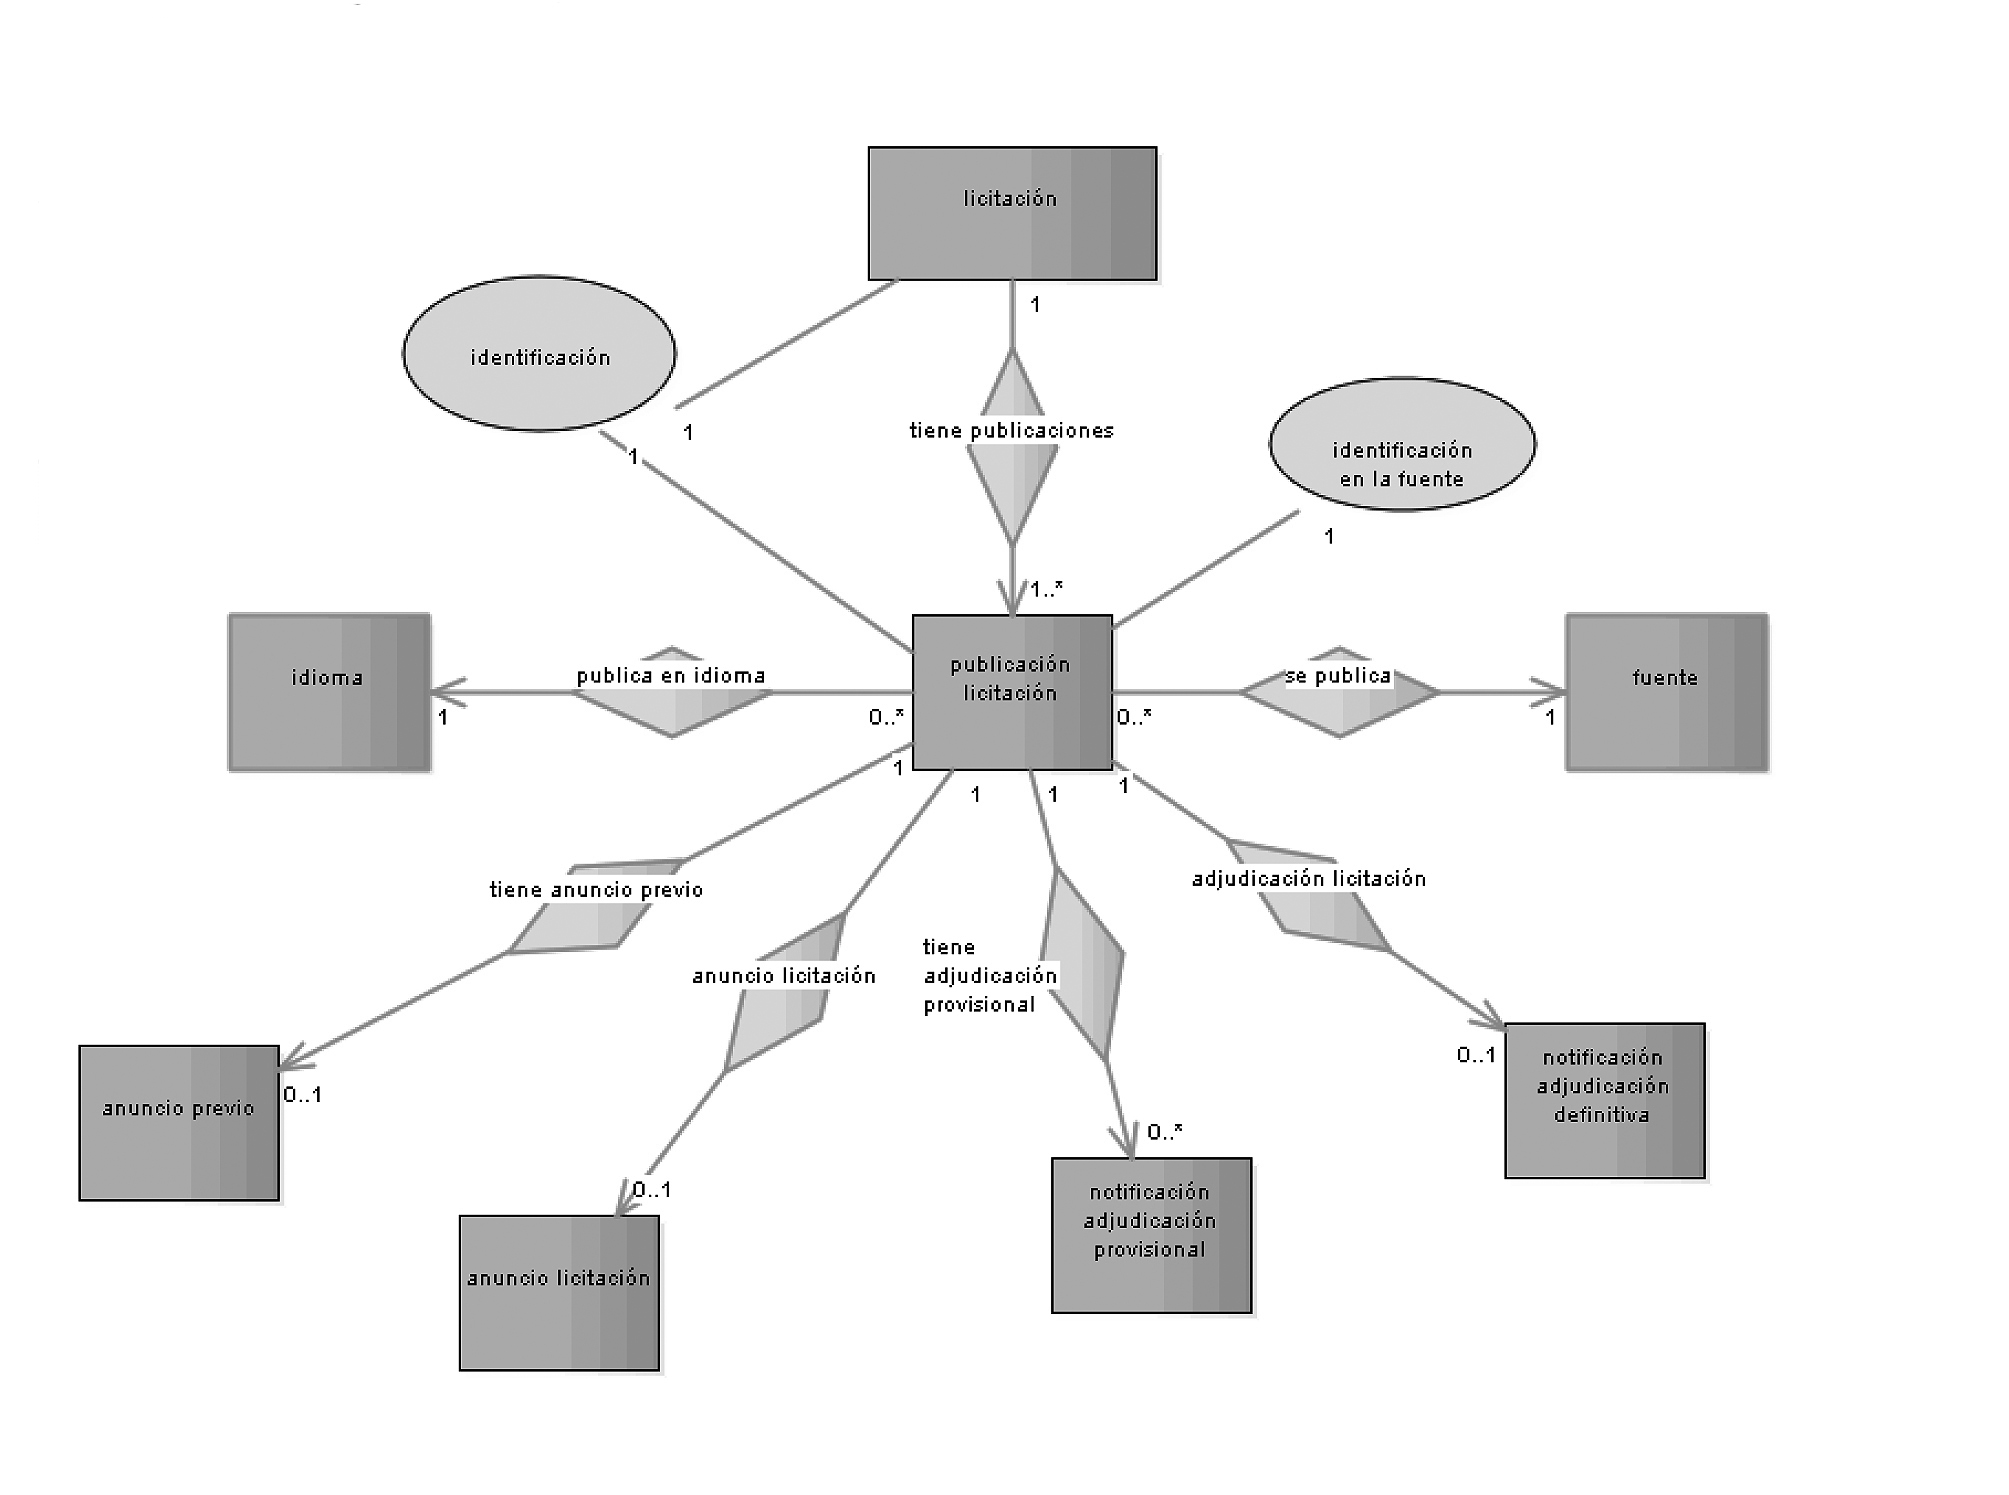
\includegraphics[width=10cm]{images/phd/eproc/10ders-1}
\caption{Publicación de Anuncio de Licitación en el proyecto 10ders.}
\label{fig:10ders-1}
\end{figure}


\begin{figure}[!htb]
\centering
	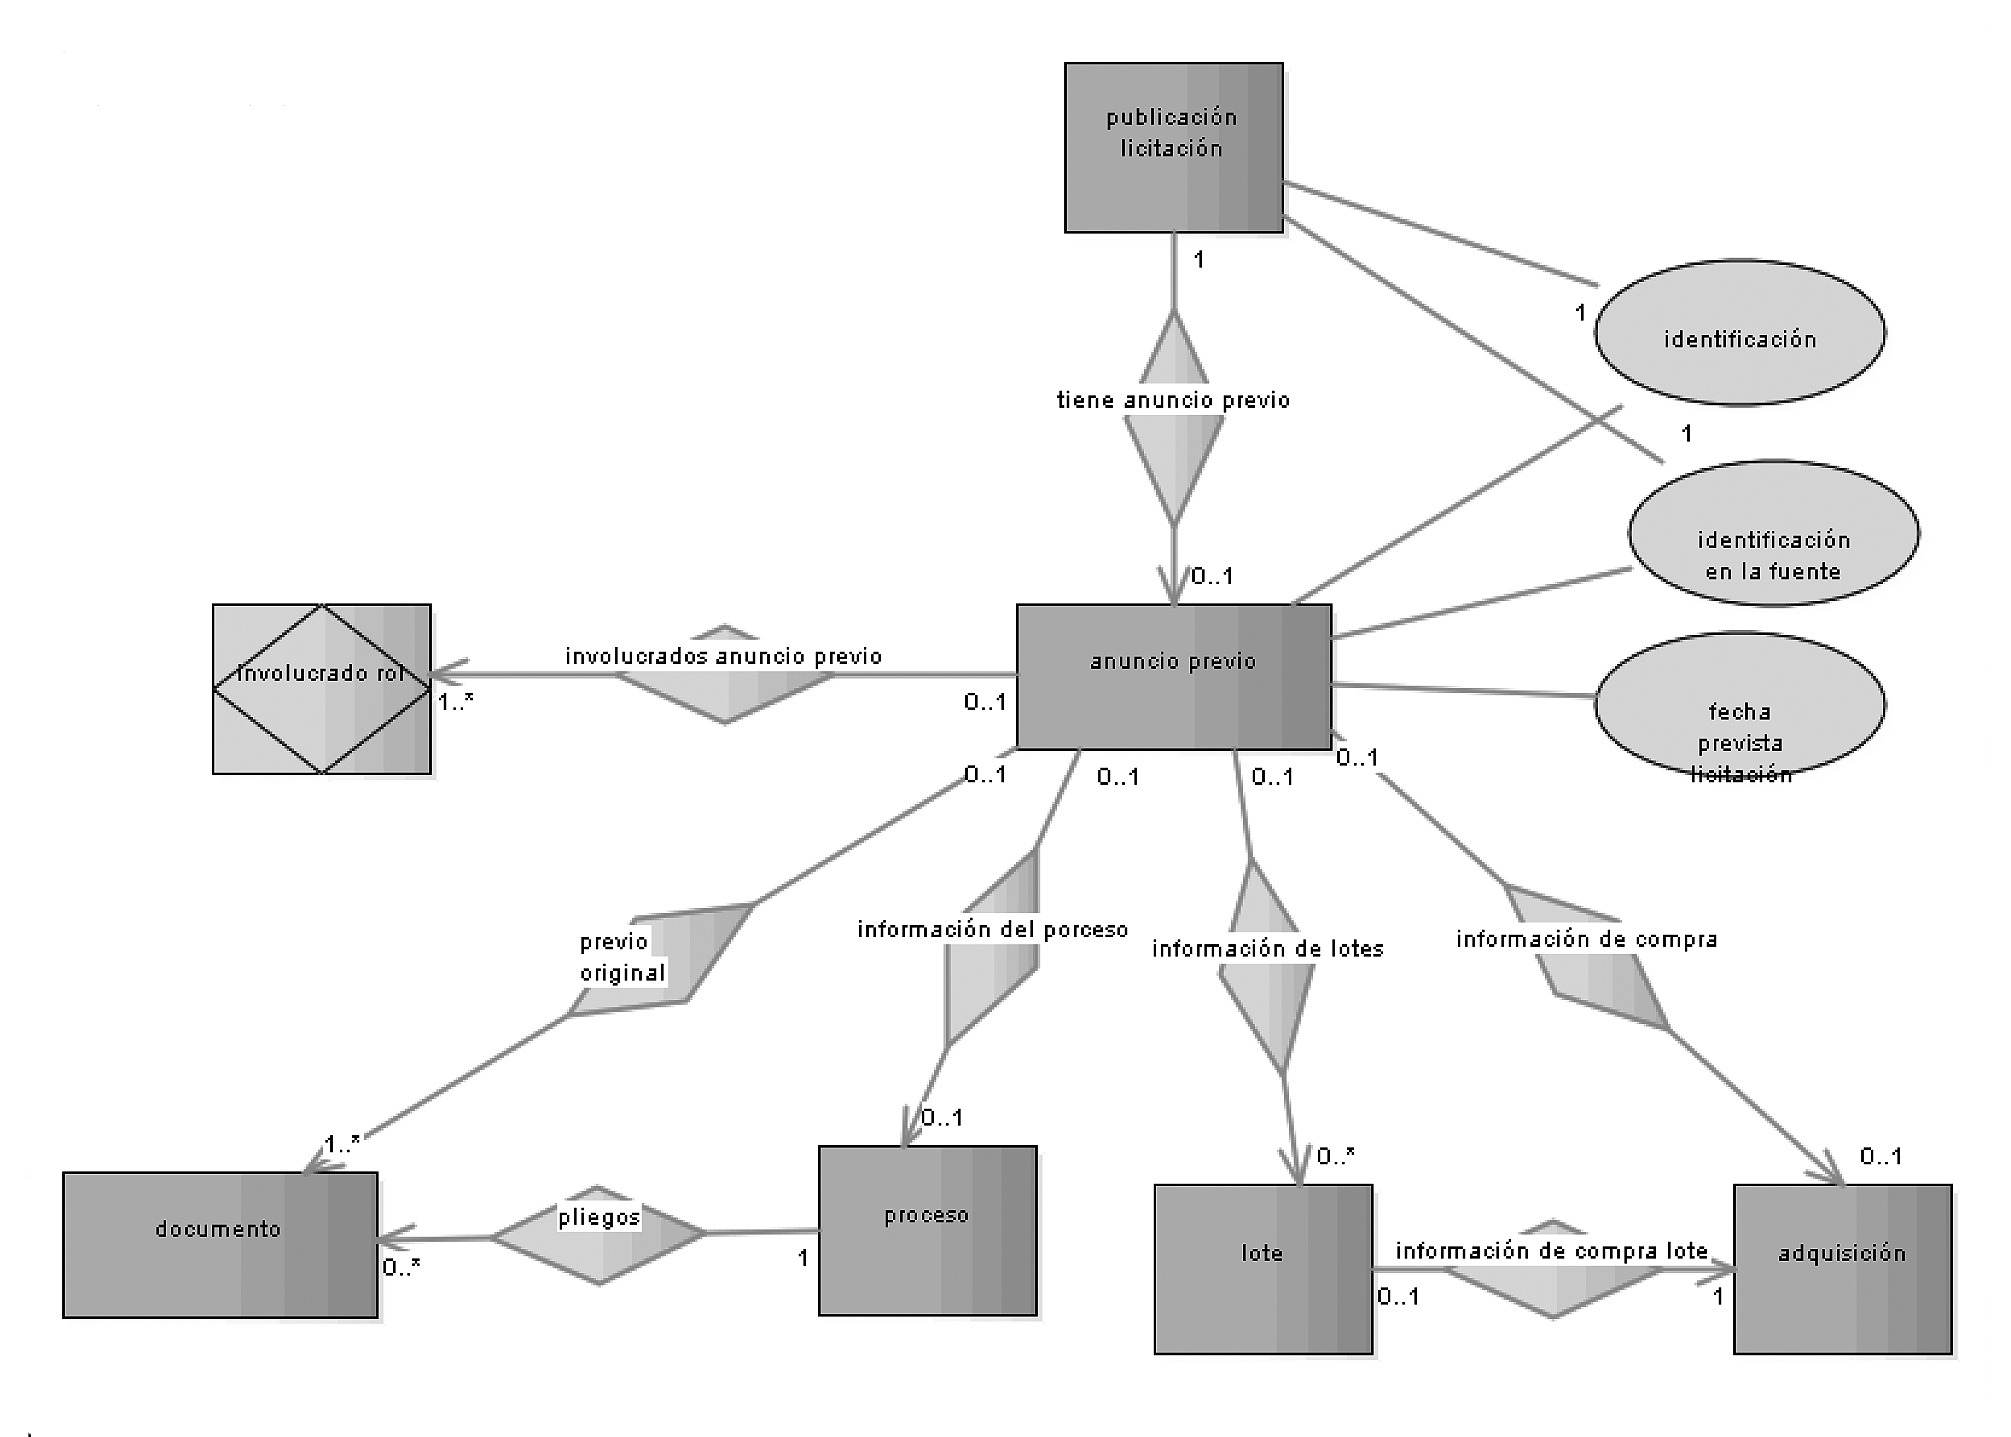
\includegraphics[width=10cm]{images/phd/eproc/10ders-2}
\caption{Anuncio Previo de Licitación en el proyecto 10ders.}
\label{fig:10ders-2}
\end{figure}


\begin{figure}[!htb]
\centering
	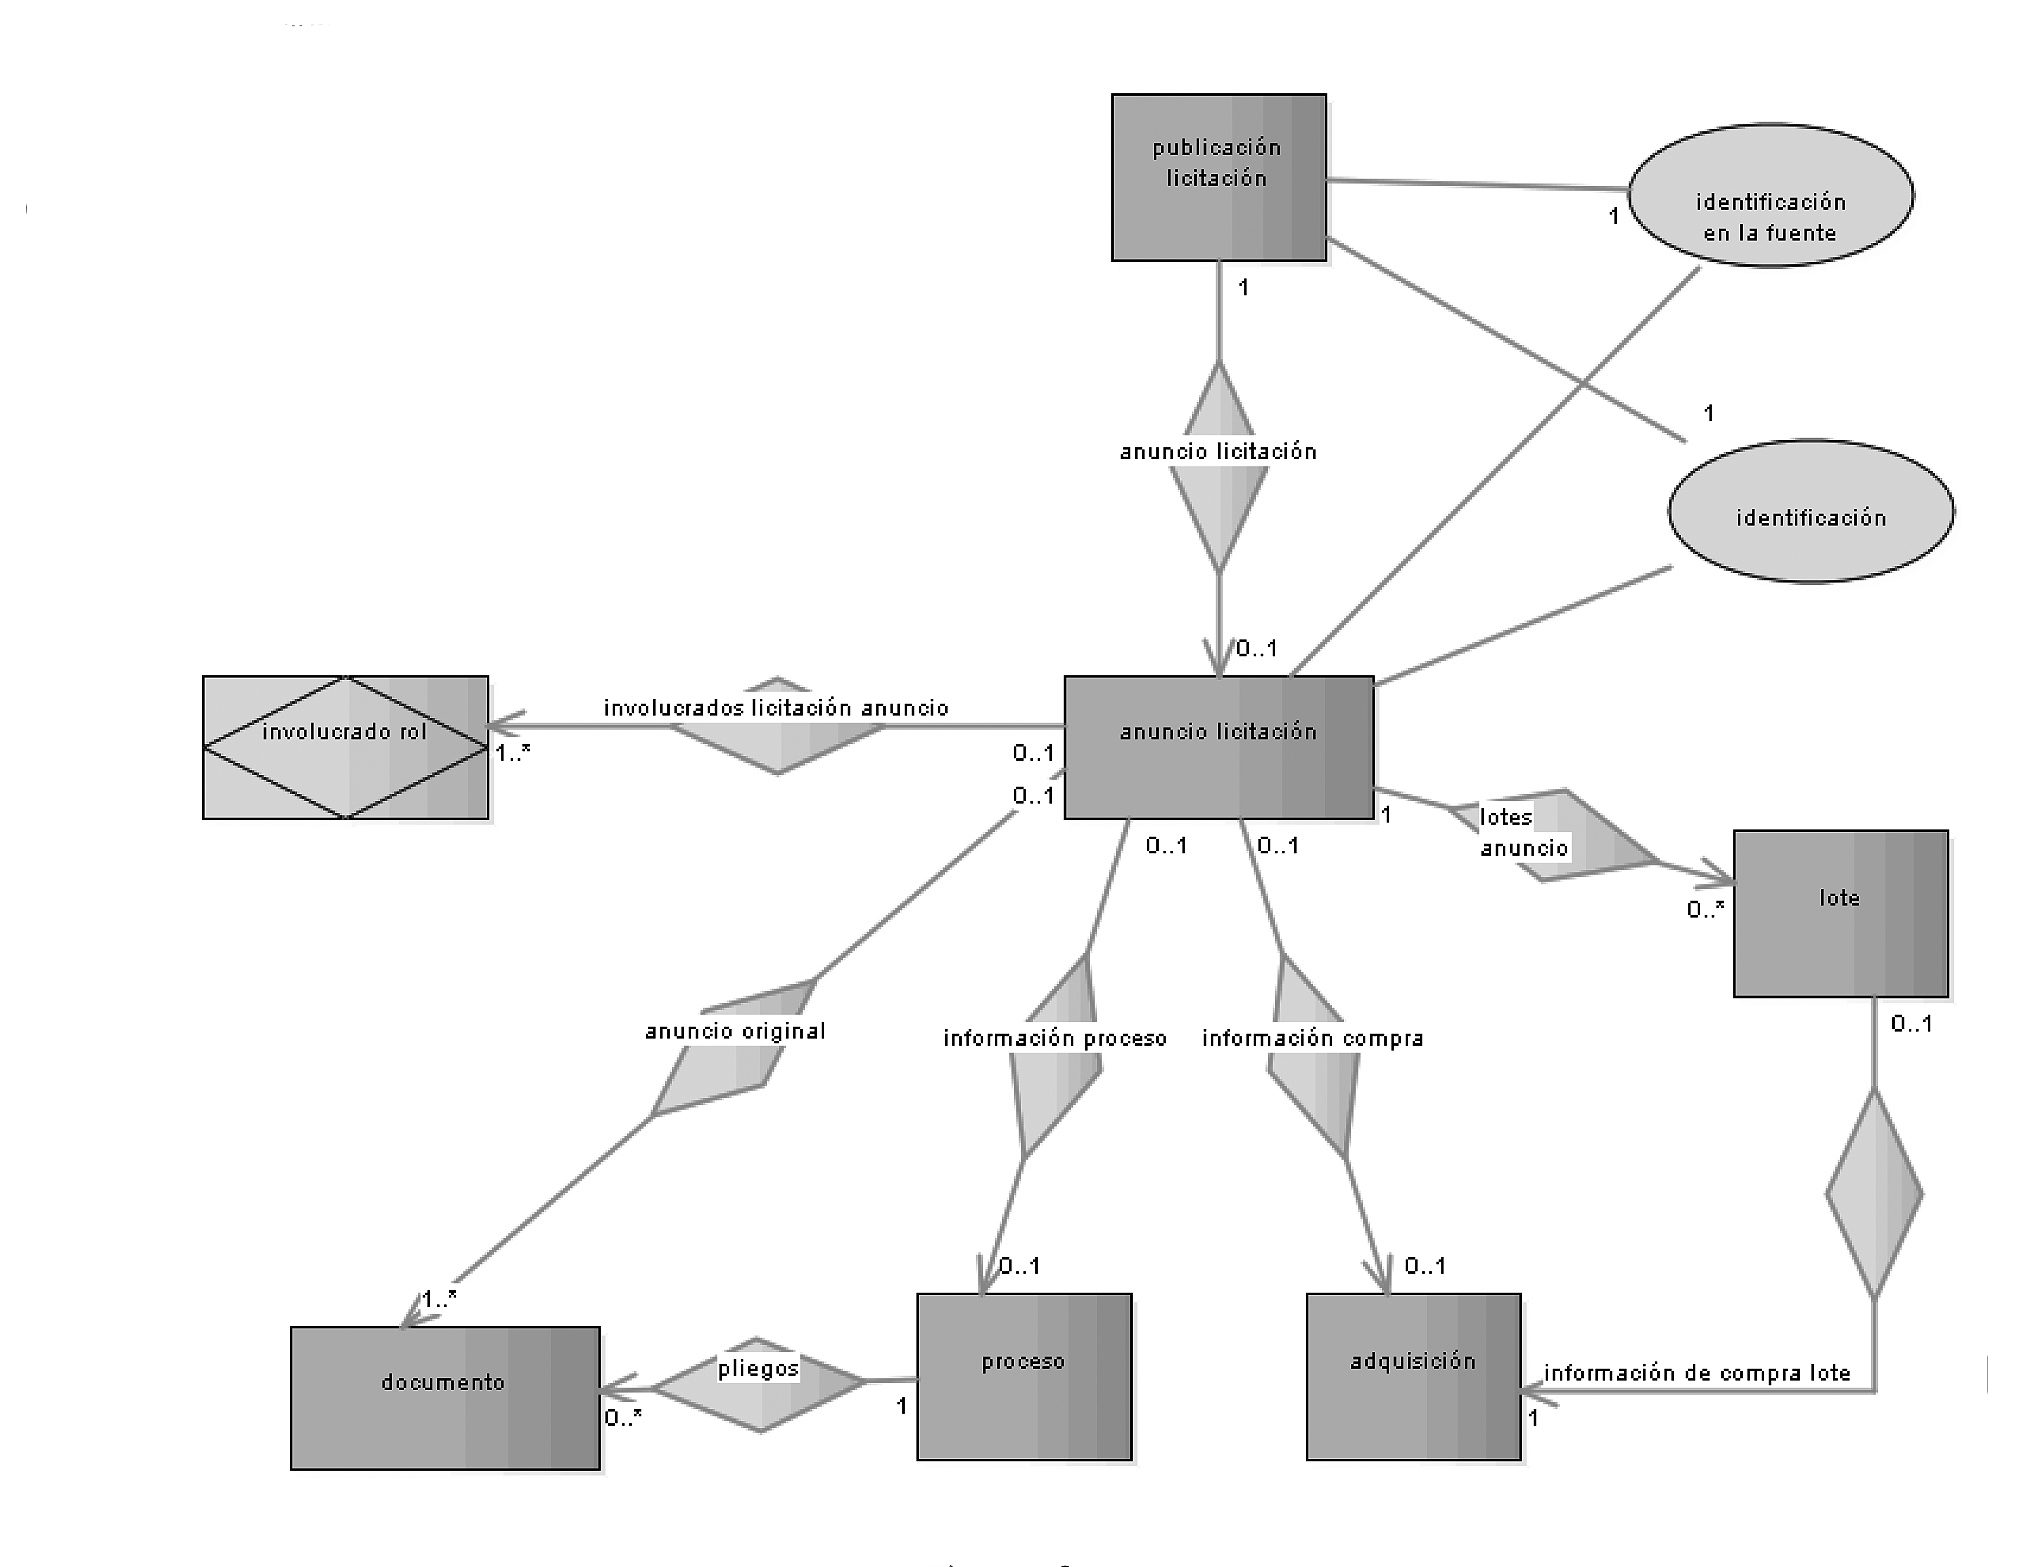
\includegraphics[width=10cm]{images/phd/eproc/10ders-3}
\caption{Anuncio de Licitación en el proyecto 10ders.}
\label{fig:10ders-3}
\end{figure}

\begin{figure}[!htb]
\centering
	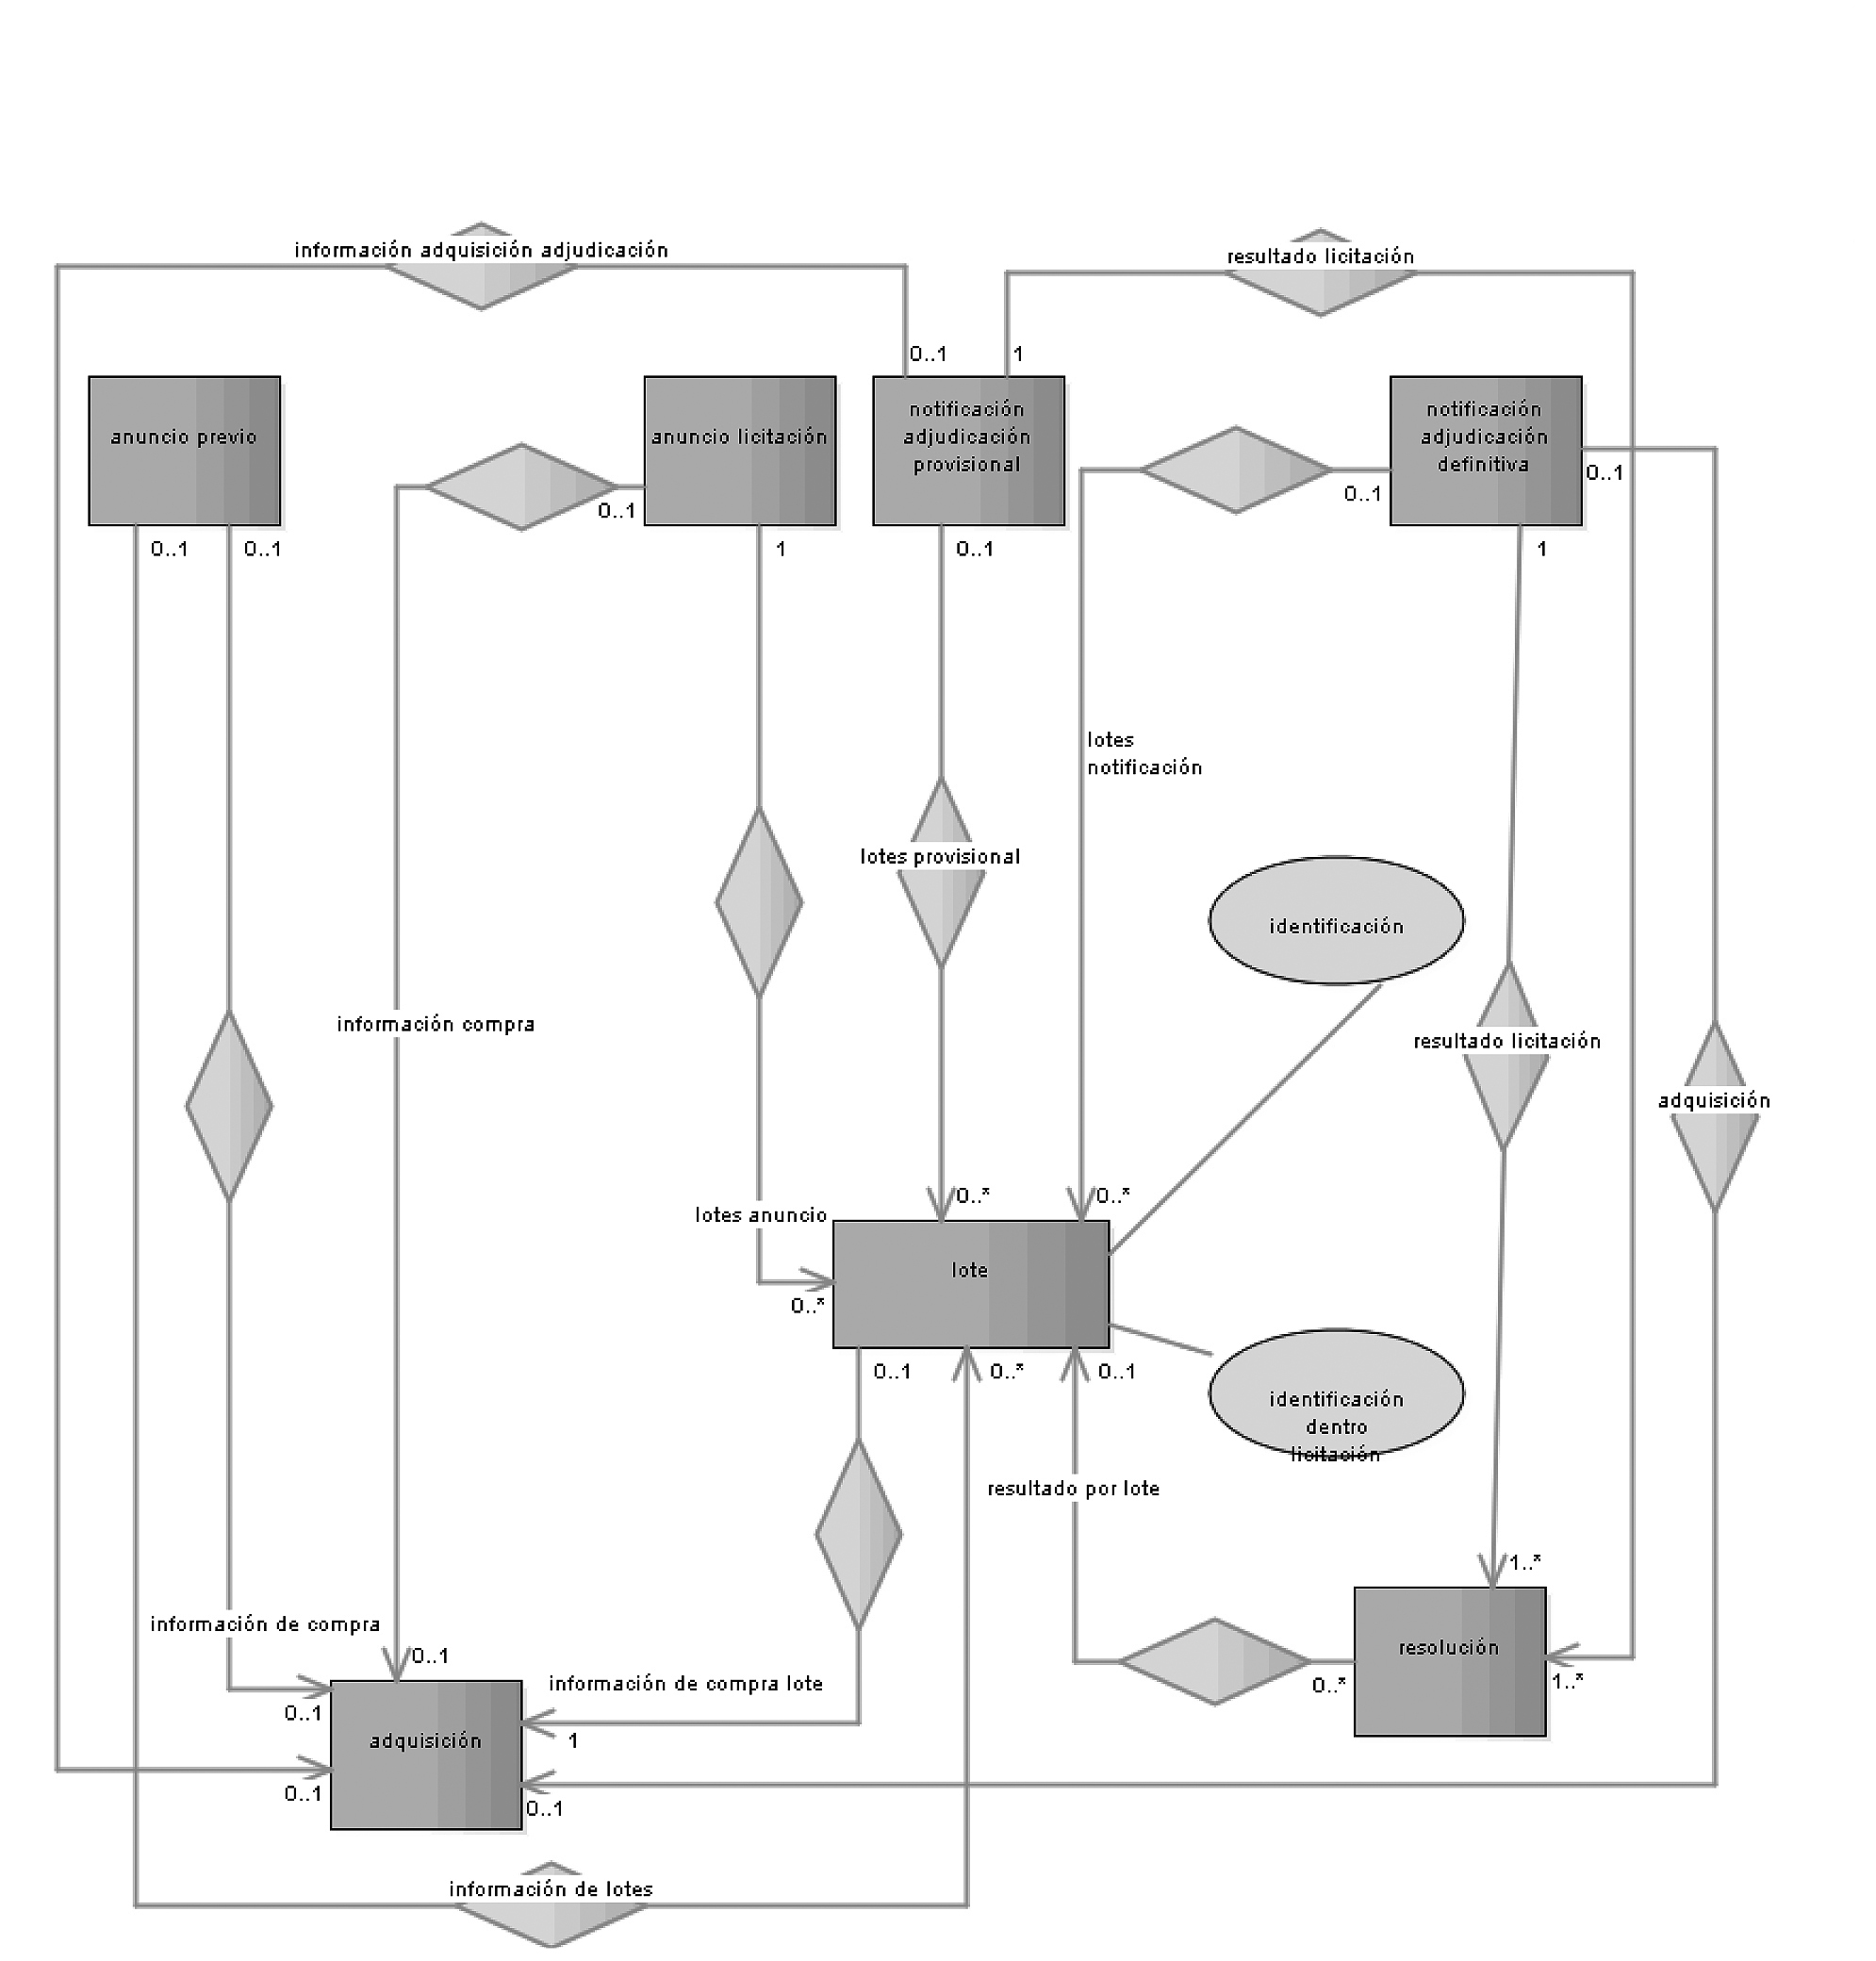
\includegraphics[width=10cm]{images/phd/eproc/10ders-6}
\caption{Lote en el proyecto 10ders.}
\label{fig:10ders-6}
\end{figure}


\begin{figure}[!htb]
\centering
	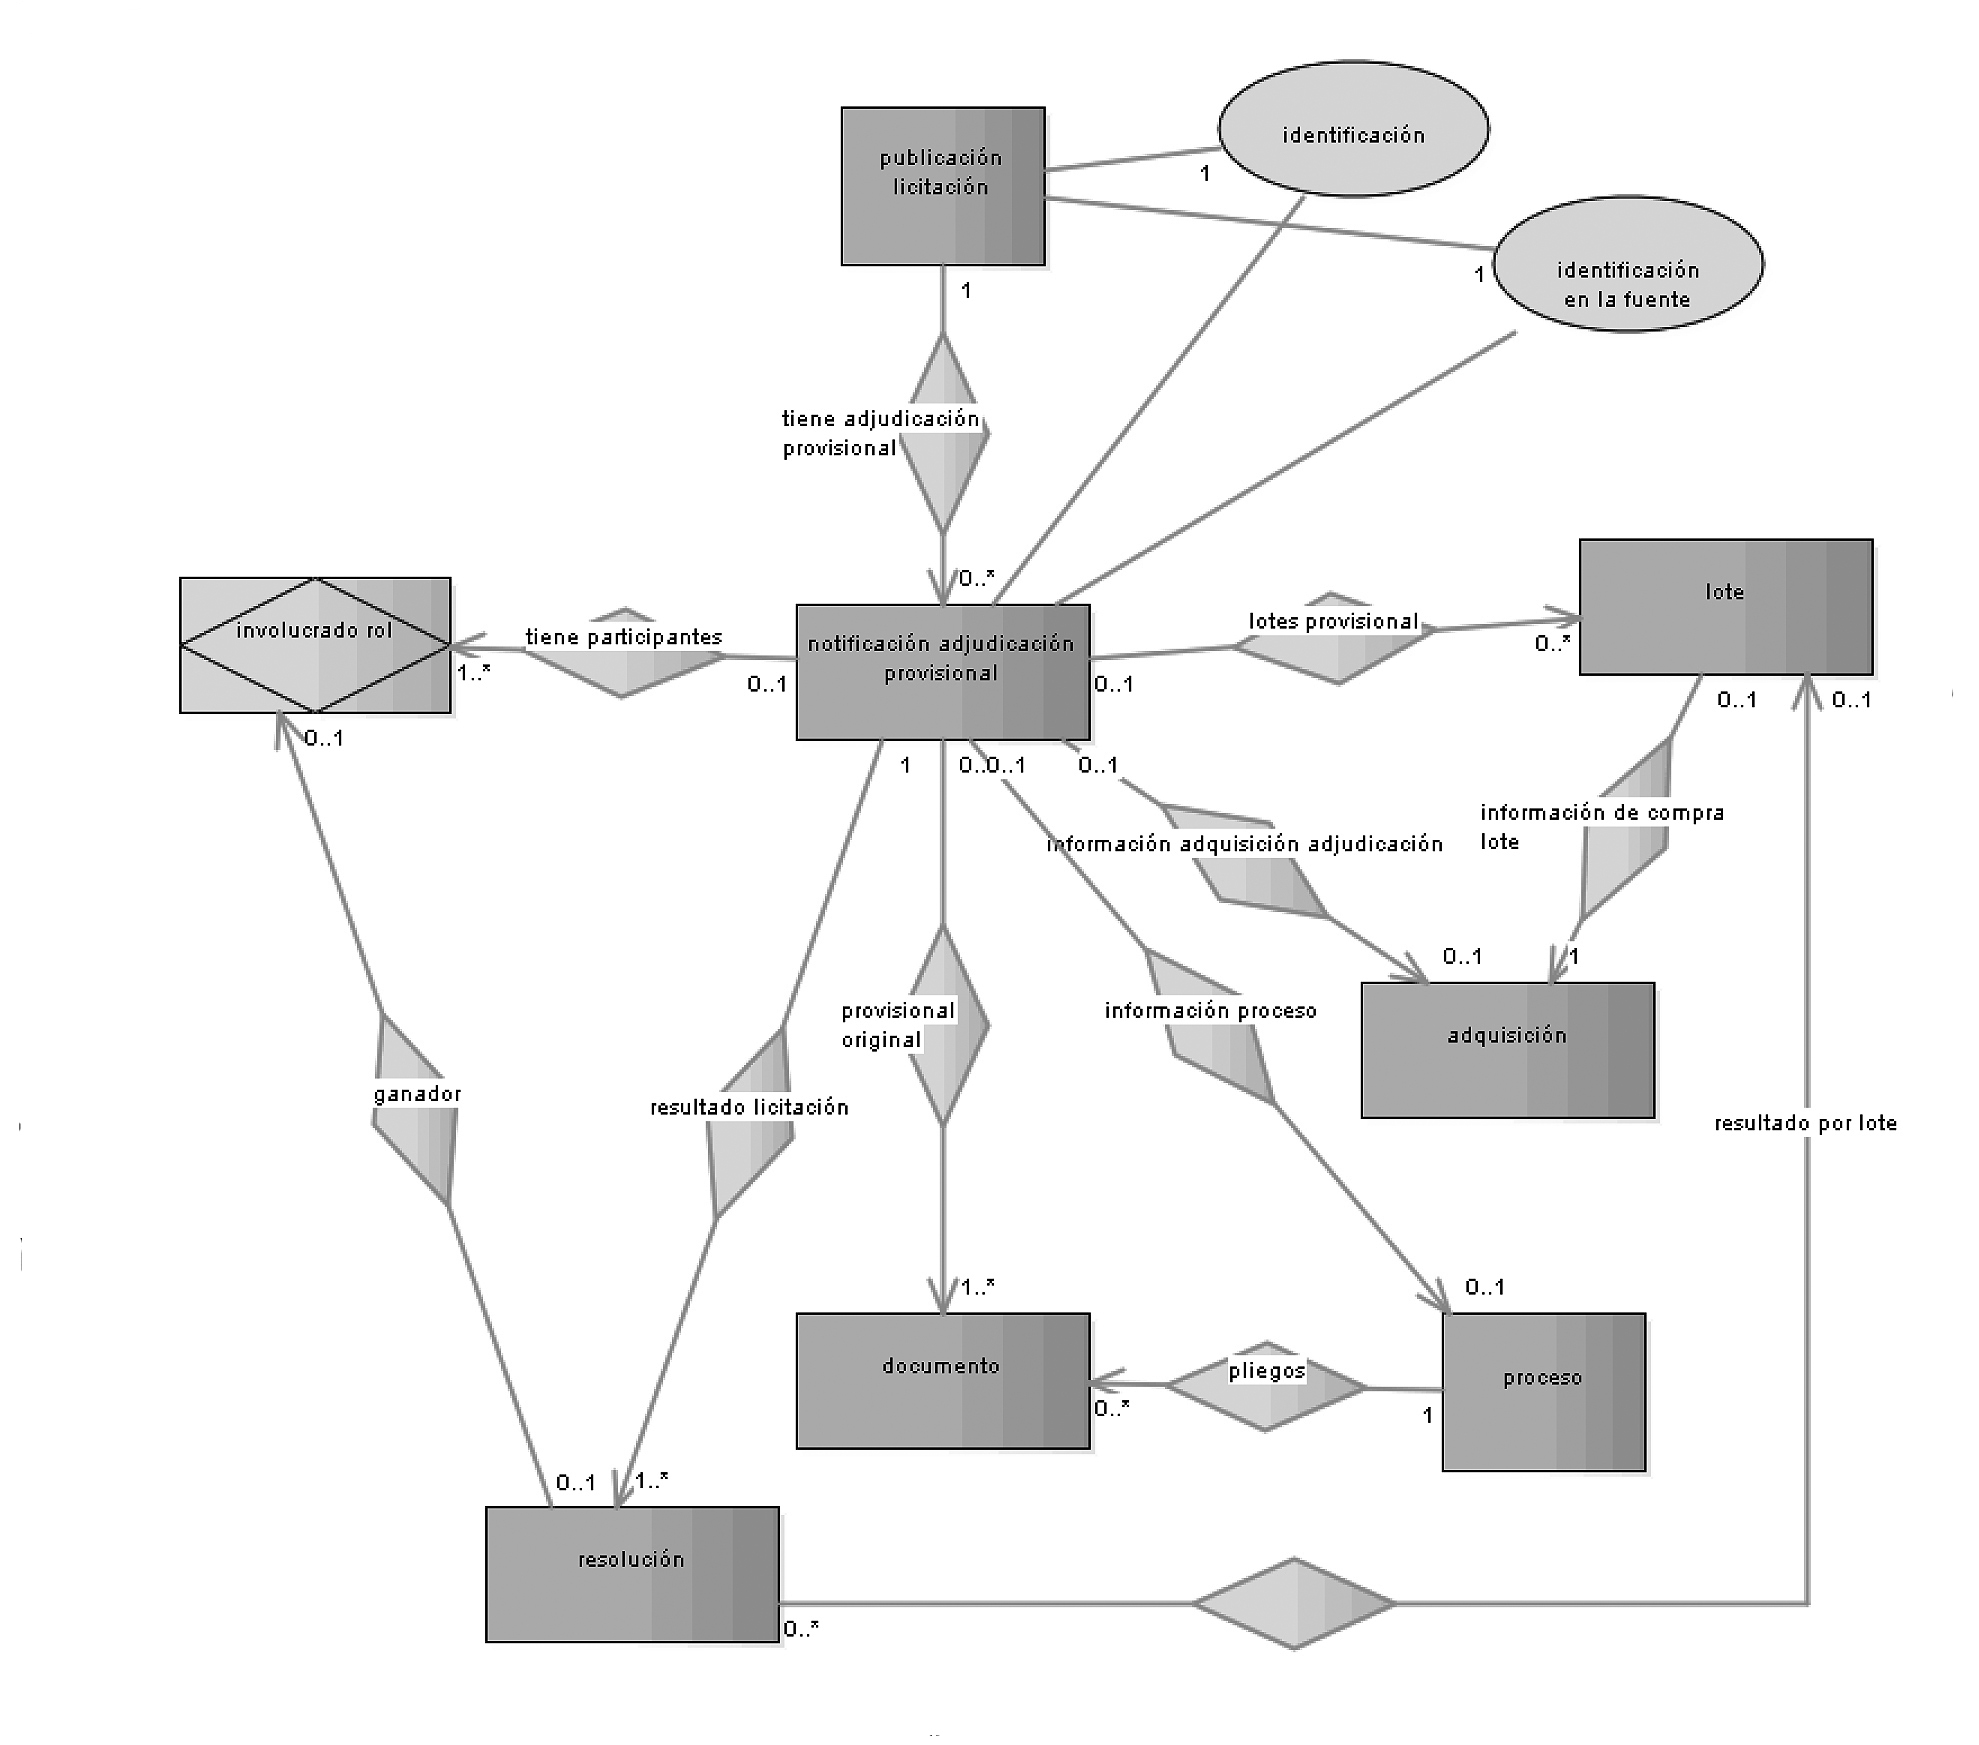
\includegraphics[width=10cm]{images/phd/eproc/10ders-4}
\caption{Notificación de Adjudicación Provisional el proyecto 10ders.}
\label{fig:10ders-4}
\end{figure}



\begin{figure}[!htb]
\centering
	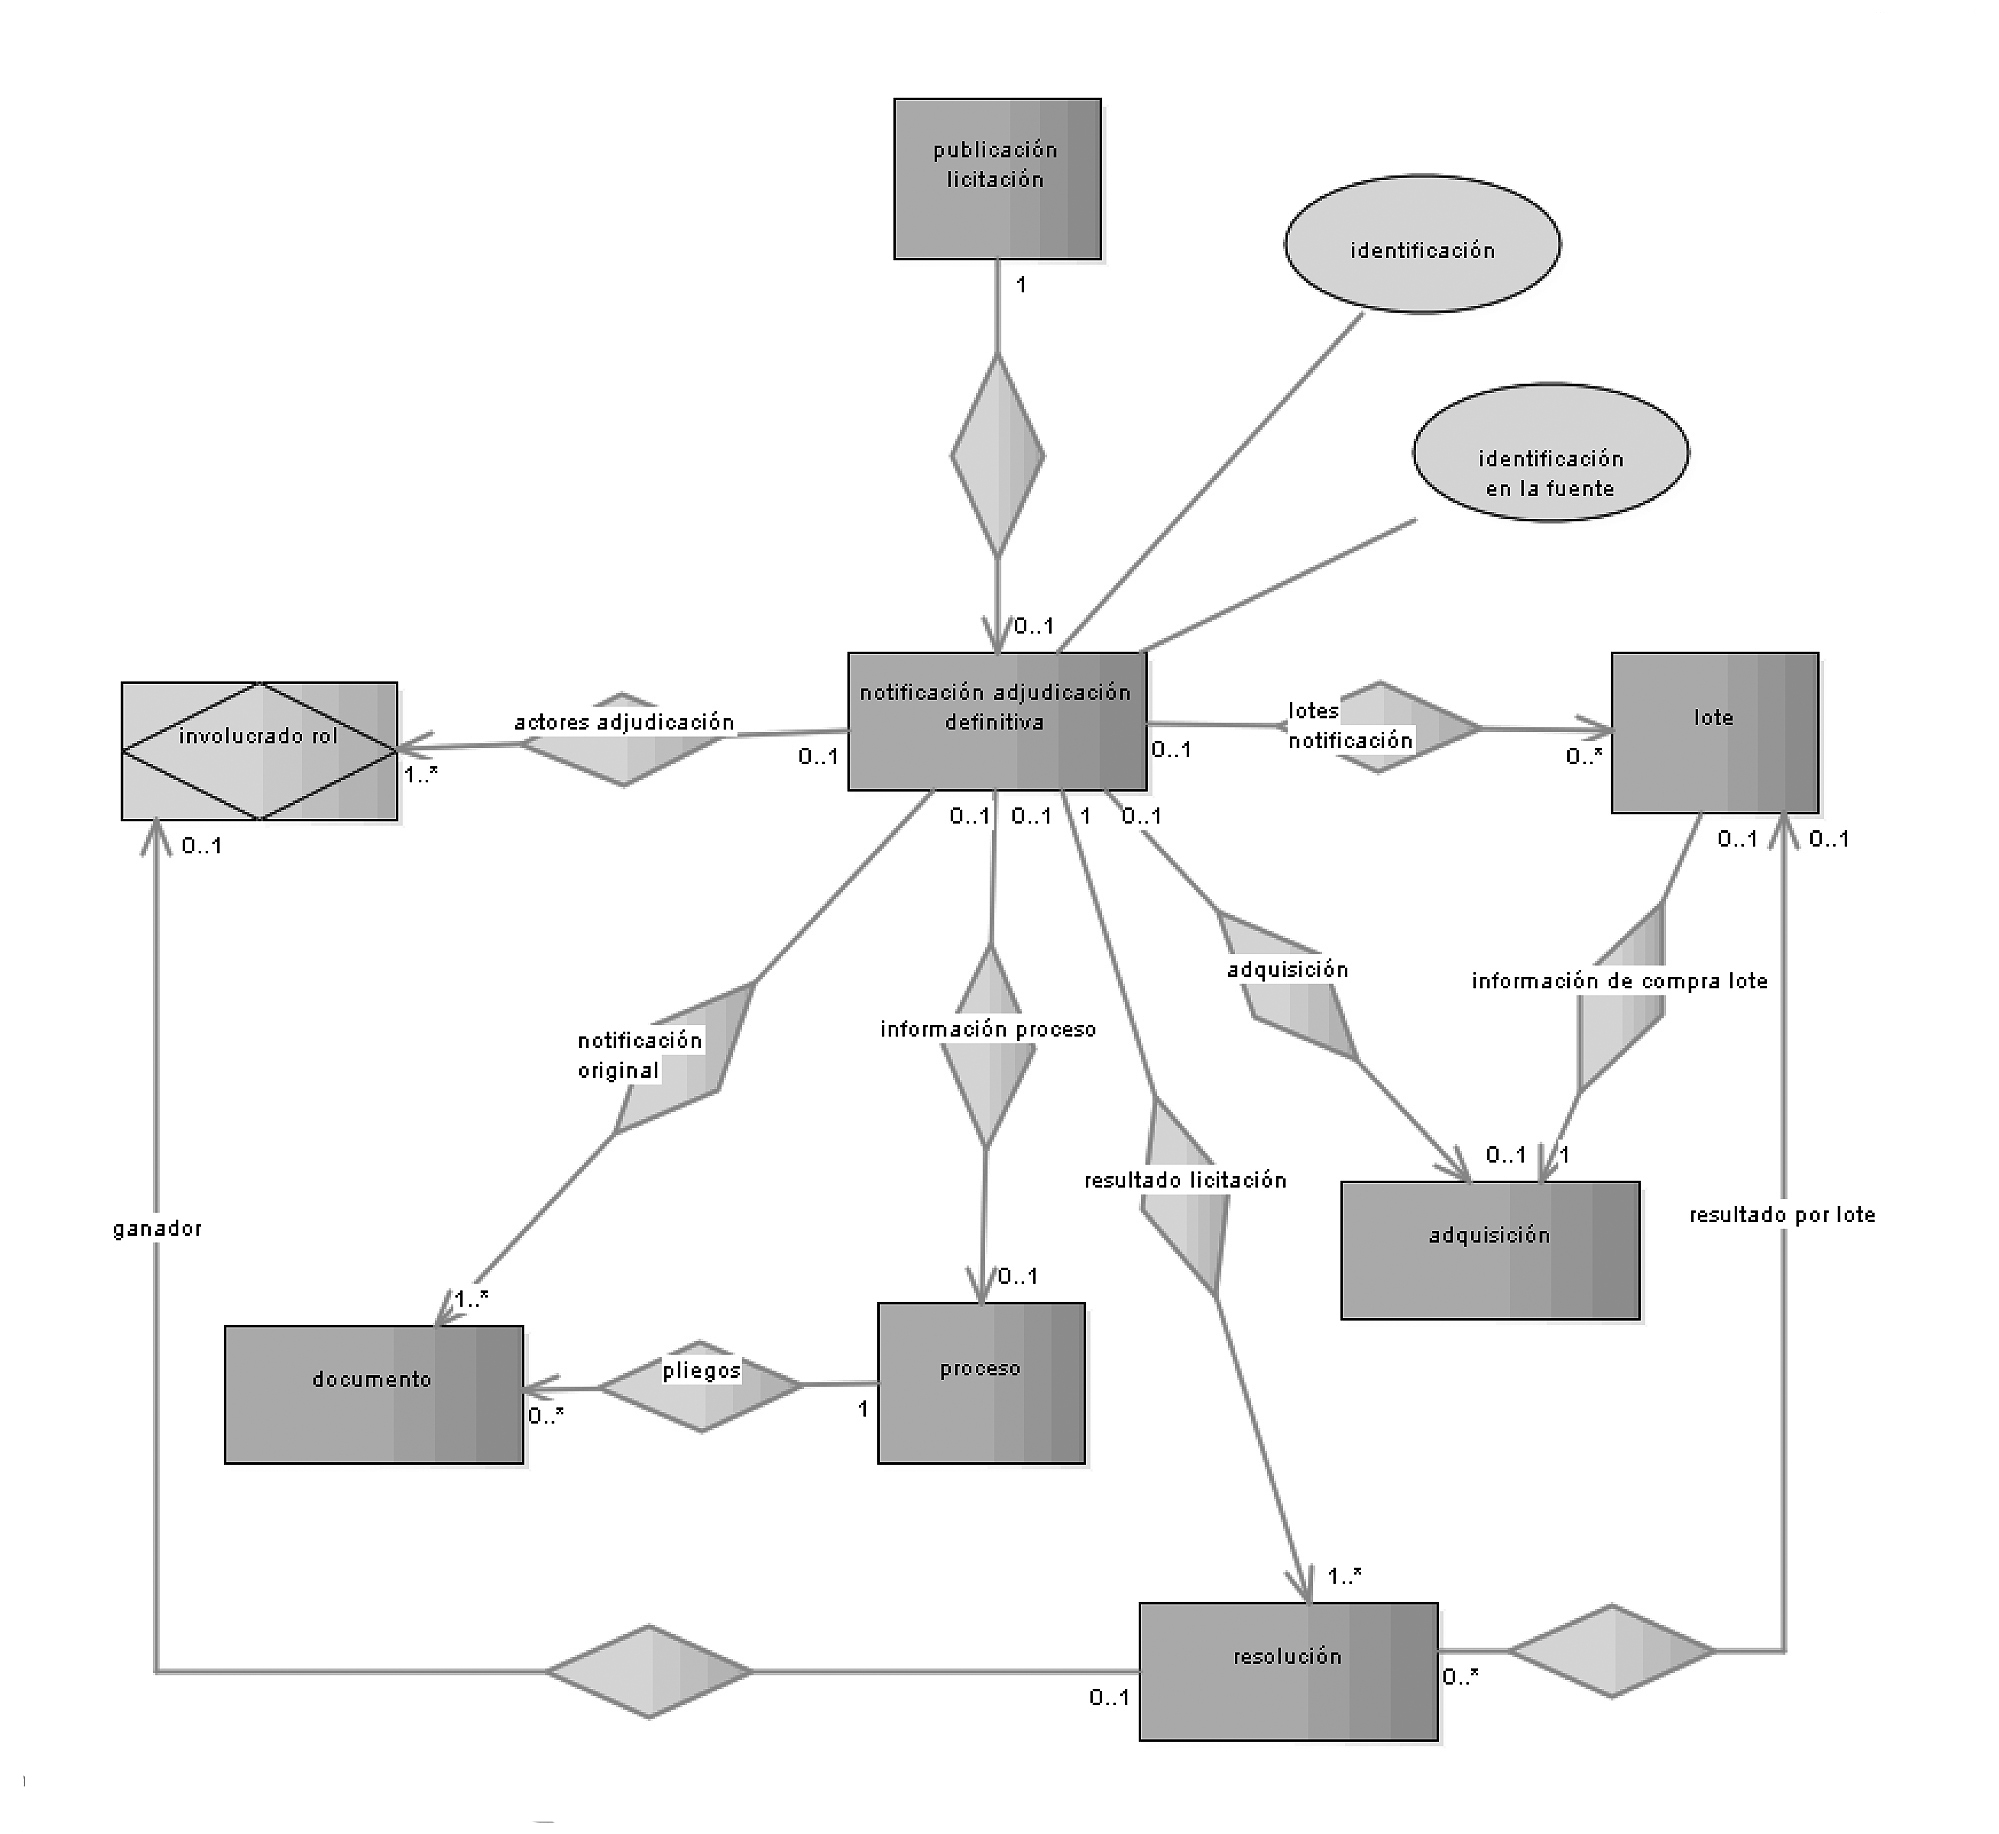
\includegraphics[width=10cm]{images/phd/eproc/10ders-5}
\caption{Notificación de Adjudicación Definitiva el proyecto 10ders.}
\label{fig:10ders-5}
\end{figure}



\begin{figure}[!htb]
\centering
	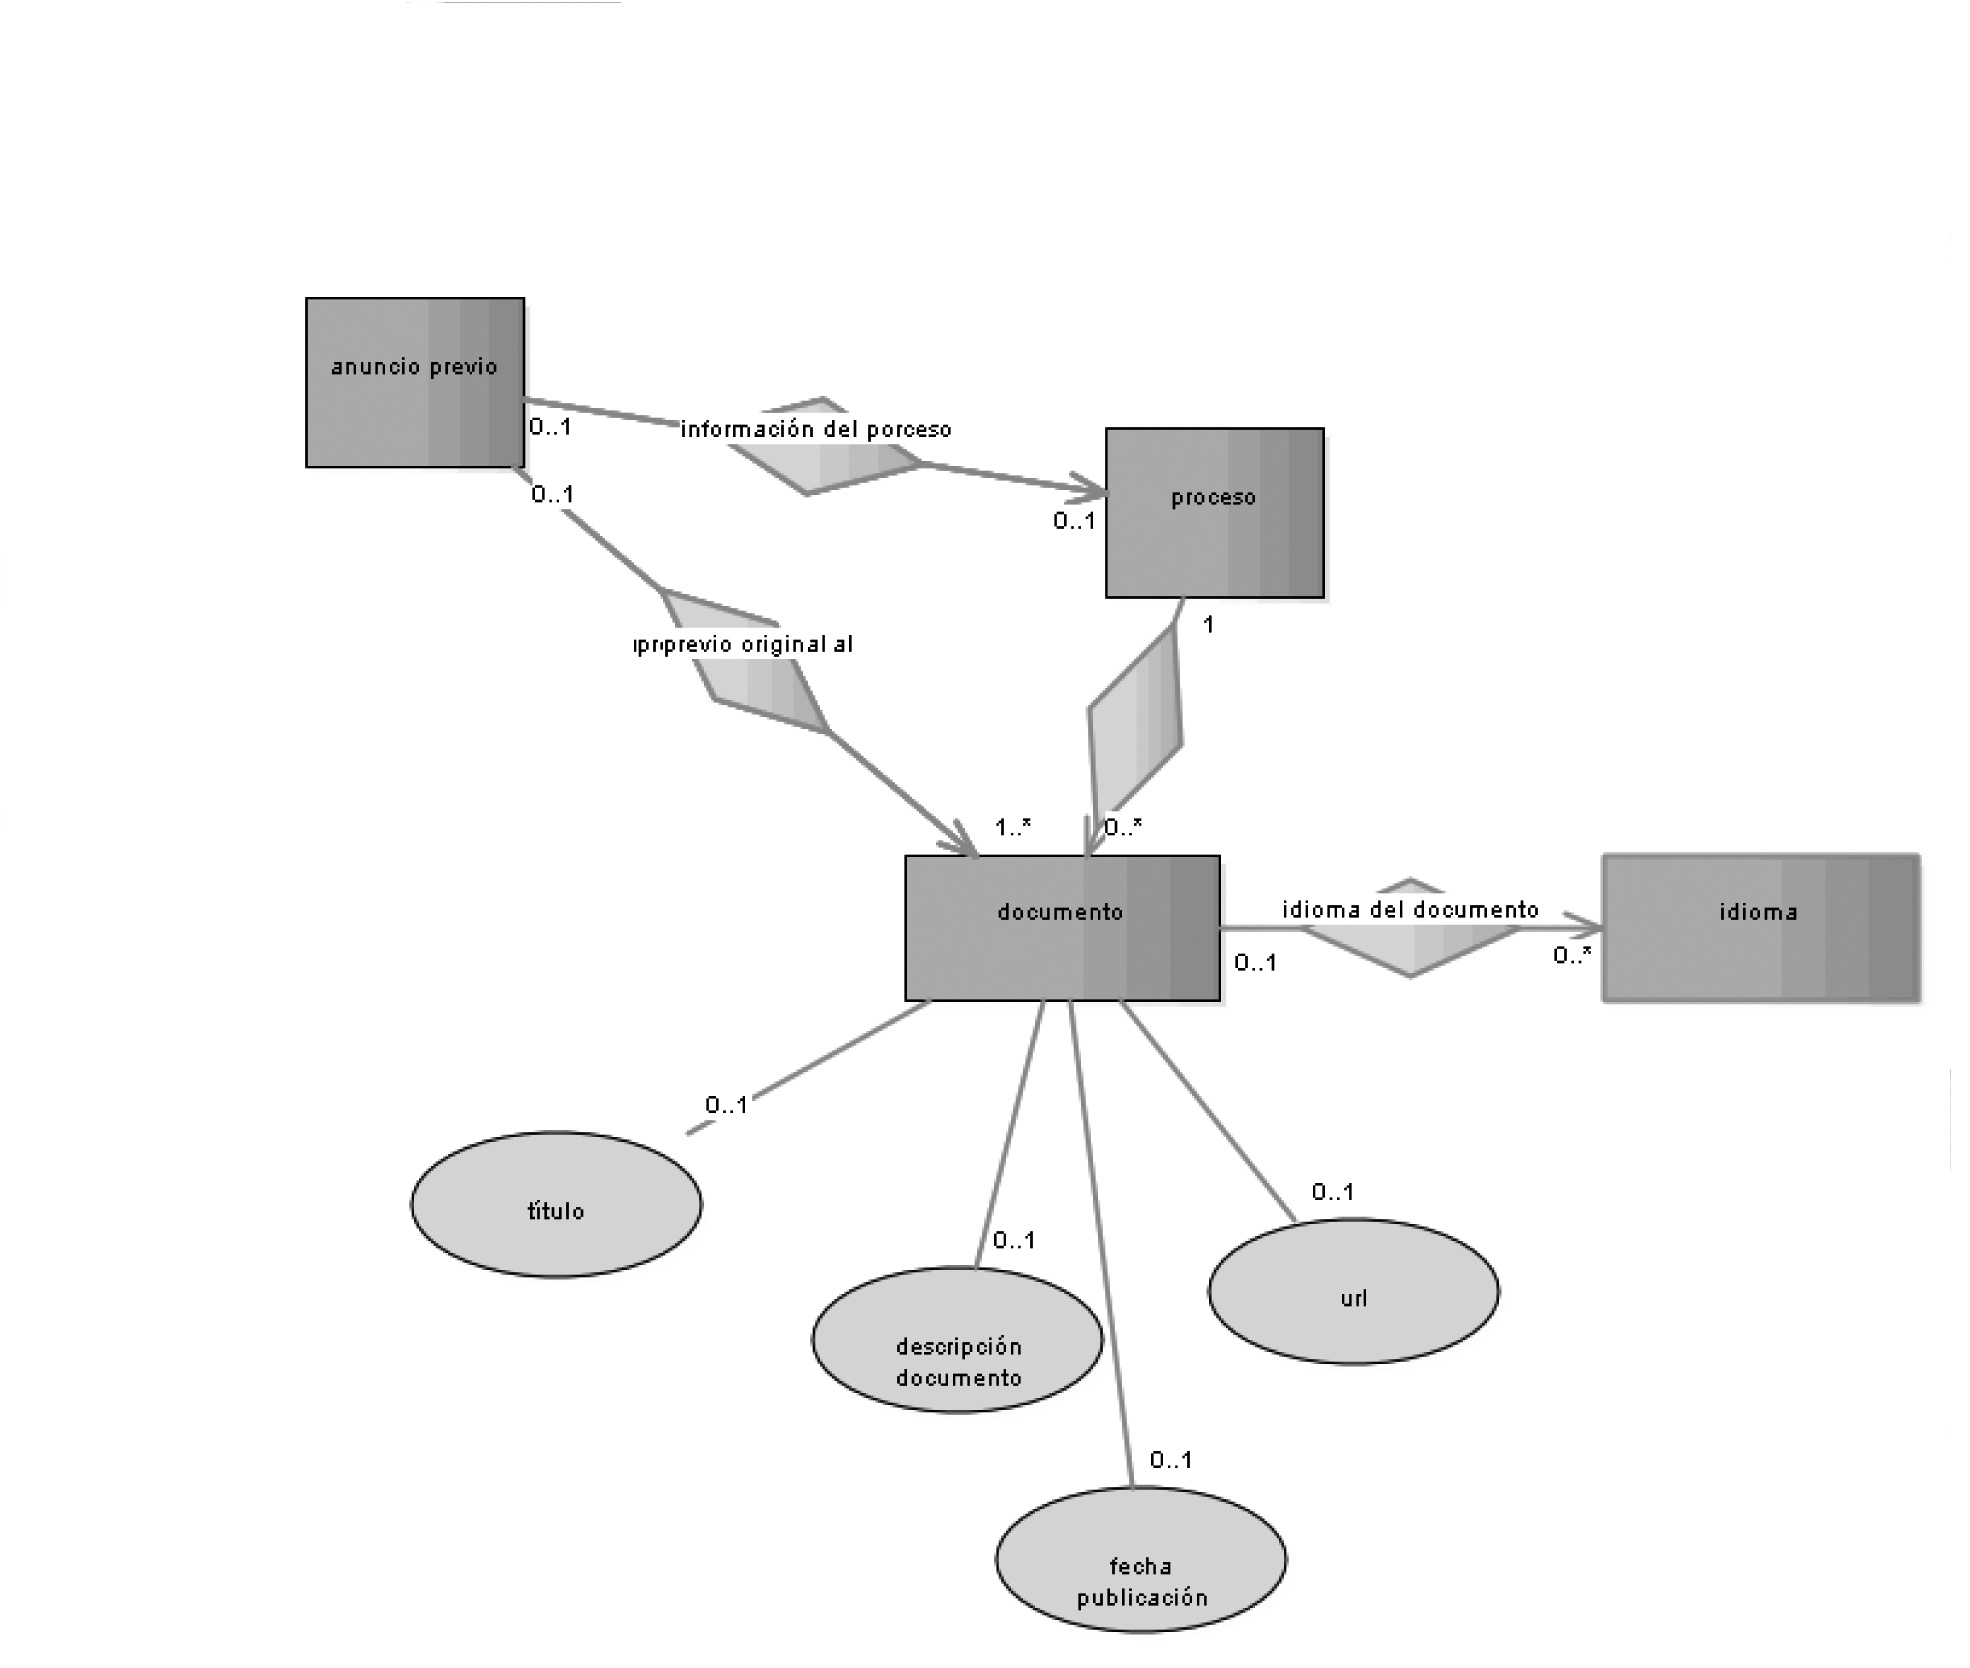
\includegraphics[width=10cm]{images/phd/eproc/10ders-7}
\caption{Documento en el proyecto 10ders.}
\label{fig:10ders-7}
\end{figure}


% 


% 











\chapter{\label{capitulo:semantica}Panorámica de uso de la\\ Web Semántica y \linkeddata} 
\epigraph{¿Por qué esta magnífica tecnología científica, \\ que ahorra trabajo y nos hace la vida mas fácil, \\ nos aporta tan poca felicidad? La repuesta es simplemente: \\ porque aún no hemos aprendido a usarla con tino.}
{\textit{Citas Célebres}\\ \textsc{Albert Einstein}}
% 30-50
\section{Web Semántica}\label{semantica}
Government bodies and public institutions as a whole are the most important buyers in the European Union (EU), since public procurement spending represents around 19\% of 
EU Gross Domestic Product (GDP)~\cite{d2010}. Given this situation there is a growing interest and commitment~\cite{d2010a} to ensure that these funds are 
well managed and most of inefficiencies are eliminated. Electronic public procurement or e-Procurement~\cite{Podlogar2007} emerges as an alternative to link and 
integrate inter-organizational business processes and systems with the automation of the requisitioning, the approval purchase order 
management, accounting processes among others through the Internet-based protocol. However there is much more at stake than the mere changeover 
from paper based systems to ones using electronic communications. It should have the potential to yield important improvements in the access to information and data such as the efficiency of individual purchases, 
the overall administration of public procurement or the functioning of the markets for government contracts. 

In this context the European Commission (EC) is trying to unlock this potential, the 2004 Public Procurement Directives 2004/17/EC and 2004/18/EC 
introduced several provisions and projects~\cite{peppol,e-certis} aimed at enabling e-Procurement uptake in all Member States. In this light of 
modernizing the European public procurement sector to support growth and employment the EC also identified~\cite{siemensEval} 
both regulatory and natural barriers in the access to public procurement in the EU context, especially for SMEs. 
According to this evaluation, a real European Single Market use~\cite{d2011} has not yet been achieved causing losses, 
being cost-inefficient, missing opportunities for society and leading to a situation where more than 27 national markets co-exist instead of an EU-wide public market~\cite{monti2010}. 
In this sense, one relevant action to ease the interconnectivity and interoperability in this landscape was the creation of the Tenders Electronic Daily~\cite{eNotices,formsTed} (TED) 
by the EC. It is the on-line version of the ``Supplement to the Official Journal of the European Union'', dedicated to European public procurement notices 
($1500$ new announcements every day) but a unified pan-European information system dealing with: dispersion of the information, 
duplication of the same notice in more than one source, different publishing formats, problems with regards to a multilingual environment and 
aggregation of low-value procurement opportunities, is still missing. As a consequence some of the potential advantages 
outlined by the EC~\cite{d2010} such as increased accessibility and transparency, benefits for individual procedures, 
benefits in terms of more efficient procurement administration and potential for integration of EU procurement markets cannot be reached in a 
short-term.

Furthermore other EU actions in the e-Government context have been focused on the development of conceptual/terminological maps available in the Eurostat's metadata server (RAMON): 
in the Health field, the ``European Schedule of Occupational Diseases'' or  the ``International Classification of Diseases''; in the Education field,  
thesauri as the ``European Education Thesaurus''; in the Employment field, the ``International Standard Classification of Occupations''; 
in the European Parliament activities the ``Eurovoc Thesaurus'' and in the e-Procurement field the ``Common Procurement Vocabulary'' (CPV). 
The structure and features of these systems are very heterogeneous, although some common aspects can be found in all of them: hierarchical relationships between terms or concepts and multilingual character of the information. 
These knowledge organization systems (KOS) enable users to annotate information objects providing an agile mechanism for performing 
tasks such as exploration, searching, automatic classification or reasoning. Nevertheless depending on the country and the scope 
distinct classifications are commonly used. In the specific case of e-Procurement, the United Nations Standard Products and Services Code (UNSPSC) in Australia, 
the North American Industry Classification System (NAICS) in United States or the CPV and TARIC (Integrated Tariff of the European Communities) in the European Union 
are examples of similar efforts to unify and model procurement-related data. As a consequence a real, standardized and integrated environment 
for e-Procurement (and business) data to encourage the creation of knowledge-based services cannot be easily deployed. In this sense the 
``European Code of Best Practices Facilitating Access by SMEs to Public Procurement Contracts''~\cite{d2008} pointed out 
two groups of difficulties regarding the barriers faced by SMEs in accessing relevant information about public procurement opportunities. 
The document stated that ``the (big) number of such web portals being used by the government and by regional and local authorities makes it difficult 
for tenderers to maintain an overview''. By aggregating data on public procurement in all Member States 
and at all administrative levels in a standardized way and reusing existing efforts of modeling 
and classifying domain knowledge, some open and critical issues can be tackled to improve a situation which affects more 
than \euro $20$ million non-financial companies established in the EU.


On the other hand and following the principles of the Open Data initiative, the vice-president Neelie Kroes is leading the Open Data Strategy for Europe. 
She also outlined in December 2011 several types of actions that will help to unleash potential of data held by governments in Europe. The strategy is 
strongly focused on the commercial value of the re-use of Public Sector Information (PSI), by which the Commission expects to deliver a \euro 40 billion boost to the EU's economy each year. 
A new version of the 2003 Public Sector Information Directive~\cite{d2003} is also expected and the EC is strongly determined to act as a global leader along with United States, 
Canada or Australia. This open data is supposed to enable greater transparency; delivers more efficient public services; and encourages greater 
public and commercial use. More specifically in the context of e-Procurement the access to public contracts announcements is the first natural 
step to encourage SME participation and create a real public market of procurement opportunities.


Moreover, the emerging Web of Data and the sheer mass of information now available make it possible the deployment of new 
added-value services and applications based on the reuse of existing vocabularies and datasets. 
The popular diagram of the Linked Data Cloud~\cite{linked-data-cloud}, generated from metadata extracted from the 
Comprehensive Knowledge Archive Network (CKAN) out, contains $336$ datasets, with more than 25 billion RDF triples and 395 million links. 
With regards to e-Procurement, a new group of 130 CKAN datasets have been released from the ``OpenSpending.org'' site. In this realm, 
data coming from different sources and domains have been promoted following the principles of the 
Linked Data initiative~\cite{Berners-Lee-2006} to improve the access to large documental databases, 
e.g. e-Government resources, scientific publications or e-Health records. In the case of KOS, such as thesauri, taxonomies or classification systems 
are developed by specific communities and institutions in order to organize huge collections of information objects. 
These vocabularies allow users to annotate~\cite{Leukel-standard,Leukel-automating,Leukel-comparative} the information objects and easily retrieve them, 
promoting lightweight reasoning in the Semantic Web. Topic or subject indexing is an easy way to introduce machine-readable metadata for a resource's content 
description. Indeed, Product Scheme Classifications (also known as PSCs), such as the CPV, are a kind of KOS that have been built to solve specific problems 
of interoperability and communication between e-Commerce agents~\cite{FenselOmel2001,Leukel-findings}, in the particular case of PSCs they are considered to be a key-enabler of 
the next European e-Procurement domain and other supply chain processes~\cite{DBLP:journals/tcci/Alor-HernandezAJPRMBG10}.

Obviously the public information published by governmental contracting authorities, more specifically PSCs, are a suitable candidate to apply the Linked (Open) Data 
(LOD) principles and semantic web technologies providing a new environment in which the conjunction of these initiatives can provide the building blocks for an 
innovative unified pan-European information system that encourages standardization of key processes and systems and gives economic operators the tools to overcome 
technical interoperability easing and enhancing the access and reuse of public information. Therefore main contributions of this paper lay in:
\begin{itemize}
\item Modeling, transforming and interlinking the structure and data of PSCs developed by public bodies following the LOD principles.
\item Publishing all information via an SPARQL endpoint providing a public procurement Linked Data node and, more specifically, a new PSCs catalogue as Linked Data.
\item Exploiting the aforementioned catalogue via a contract descriptor recommendation service.
\item Demonstrating the gain (in terms of number of descriptors to retrieve public procurement notices) and the semantic exploitation 
capabilities of the new PSCs catalogue.
\end{itemize}

The remainder of this paper is structured as follows. Section~\ref{sect:related-work} reviews the relevant literature. Next thesauri 
conversion methods are outlined. Section~\ref{sect:method} presents the application of a method for promoting raw data to the LOD initiative 
and its application to the PSCs in the European e-Procurement sector. Section~\ref{sect:evaluation} describes the evaluation of applying the LOD principles to 
these product schemes through two studies that include a description of the sample, the method, results and discussion. Finally, 
the paper ends with a discussion of research findings, limitations and some concluding remarks.
                                                                     
\subsection{Definición}                                                                                              
La Web Semántica siguiendo la definición propuesta por el W3C se presenta como: 
\begin{Frame}
\textit{Una web extendida, dotada de mayor significado, en la que cualquier
usuario en Internet podrá encontrar respuestas a sus preguntas de forma más rápida y
sencilla gracias a una información mejor definida.}
\end{Frame}

Surge como respuesta a las dificultades que aparecen al tratar de 
automatizar muchas tareas en la web actual. Hoy en día, los contenidos de la web son
creados considerando que van a ser consumidos principalmente por personas,
lo que hace difícil su interpretación por parte de agentes \textit{software}.
En consecuencia, algunas tareas comunes como la búsqueda de información en la web actual,
son notoriamente mejorables; otras tareas aparentemente sencillas son casi imposibles de implementar.
En el origen de este problema se encuentra la incapacidad de los agentes \textit{software} (las máquinas)
para encontrar, interpretar, extraer y combinar la información ya disponible en la web.


Para tratar de paliar esta situación, \textit{Tim Berners-Lee}, reconocido como ``padre de la web'',
impulsa a través del \gls{W3C} el desarrollo de la Web Semántica ~\cite{WeavingTim,berners-lee06a}.
A través de esta iniciativa, se desarrollan los lenguajes y formalismos que permiten
extender la web actual, de tal manera que sus contenidos sean accesibles tanto a
personas como a máquinas. Esta tecnología abre la puerta a una nueva generación
de aplicaciones informáticas capaces de encontrar, seleccionar y combinar la
información dispersa en la web para realizar tareas que actualmente se ejecutan de forma manual: seleccionar los resultados relevantes en una búsqueda, agregar
información procedente de distintas fuentes, etc.


Una de las fortalezas de la web actual es la ingente cantidad de información que se encuentra
publicada en ella y la infinidad de servicios a los que se puede acceder.
Sin embargo, si la explotación de estos recursos requiriese necesariamente la intervención humana,
como sucede ahora, su utilidad estaría limitada, de ahí que el W3C pretenda
``guiar a la web hacia su máximo potencial'' como herramienta universal y multipropósito.
La Web Semántica proporciona una infraestructura para explotar eficientemente el potencial de
la web~\cite{Berendt02,decker00knowledge}, se encuentra, sin embargo en continuo desarrollo, gestándose gradualmente su progresión.

En el contexto de la iniciativa de la Web Semántica, se han desarrollado y se continúan
desarrollando estándares que son el soporte necesario para hacer realidad la misma.
En la base se utilizan tecnologías estándar ya asentadas, como \gls{XML}~\cite{XML11}, \gls{HTTP}~\cite{http-rfc} y \gls{URI}s~\cite{uri-rfc},
que son también la base de la web actual. Pero además se han creado nuevos mecanismos
para describir semántica y formalmente la información, se trata, entre otros, de \gls{RDF}~\cite{RDF}, \gls{RDF Schema}~\cite{RDFS} y \gls{OWL}~\cite{OWL11,owl2-primer}. Con estos lenguajes y modelos se puede describir la información de manera precisa y
y carente de ambig\"{u}edad basándose en teorías lógicas como las \textit{Description Logics~\cite{baader03description} (\gls{DL}s)}.
En este sentido juegan un papel fundamental las taxonomías, los tesauros y las ontologías,
como estructuras capaces de dotar de significado a los datos 
~\cite{Benjamins98knowledgemanagement}.

\subsubsection{No es Web Semántica}
En muchas ocasiones, no existe manera más conveniente para definir un concepto que encontrar
un contraejemplo. Así, \textit{Tim Berners-Lee} insiste en que la Web Semántica \textbf{No} es inteligencia artificial: 
\begin{Frame}
\textit{El concepto de documento entendible por una máquina no implica algún tipo de
inteligencia artificial mágica que permita a las máquinas comprender el
farfullar de los humanos. Sólo indica una habilidad de la máquina para resolver
un problema bien definido a base de realizar operaciones bien definidas sobre
unos datos bien definidos. En vez de pedir a las máquinas que entiendan nuestro
lenguaje, se le pedirá a la gente que haga un esfuerzo extra.} \textit{A roadmap
to the Semantic Web.  What the semantic Web isn't but can represent}. 1998. 

Fuente: \url{http://www.w3.org/DesignIssues/RDFnot.html}
\end{Frame}

Por tanto, desposeída de su aura mágica al no constar entre sus objetivos la
conquista del lenguaje natural, la Web Semántica queda reducida a un intercambio
de información eficiente entre los agentes.
                                                                
\subsection{Infraestructura para la Web Semántica}                                                                   
La iniciativa de la Web Semántica puede ser divergente en sus enfoques para los
diferentes escenarios de aplicación, pero lo que está perfectamente definido
es su apoyo en el uso de \textbf{ontologías}~\cite{Sowa99knowledge}. 

\subsubsection{Ontologías en la Web Semántica}
La evolución de la web a través de la Web Semántica, proporciona un nuevo
espacio de publicación de recursos (documentos) que junto con las nuevas tecnologías de
la información generan un entorno con unas condiciones inigualables para la
divulgación de contenido.

Uno de los principales problemas de la web actual es la inmensa cantidad de
información que se publica obviando cualquier procedimiento de control, creando
grandes bases de datos, recursos y conocimiento, cuya explotación no es eficiente, ya que
en muchos casos sólo está preparada para ser procesada o bien por agentes
humanos o por agentes \textit{software}.

Las ontologías se presentan como una forma para la organización de conocimiento
y contenido heterogéneo en el ámbito de la Web Semántica, estableciendo un enlace entre el procesamiento humano de recursos y el
automático, realizado entre agentes \textit{software}. Paralelamente, las ontologías se utilizan como
instrumentos para la desambiguación del lenguaje natural. Constituyendo en definitiva un mecanismo para 
la realización de la comunicación entre agentes de forma eficiente
basándose en un conocimiento común y compartido. En la Sección~\ref{ontologias} se describen más amplia y genéricamente los modelos de conocimiento basados en ontologías.

\subsubsection{Arquitectura para la Web Semántica}\label{sect:arch-ws}
En un primer momento, la arquitectura para la Web Semántica, más conocida como
``tarta o pila de la Web Semántica'', ver Figura~\ref{fig:stack-2002}, se diseño con diferentes capas de abstracción, 
construyen un \textit{framework} semántico, recogiendo supuestamente, todas las necesidades para la gestión del
conocimiento. Cada una de las capas enriquece a la inmediatamente inferior
proveyendo nuevos servicios o niveles de formalización superior del conocimiento.

\begin{figure}[!htbp]
\centering
	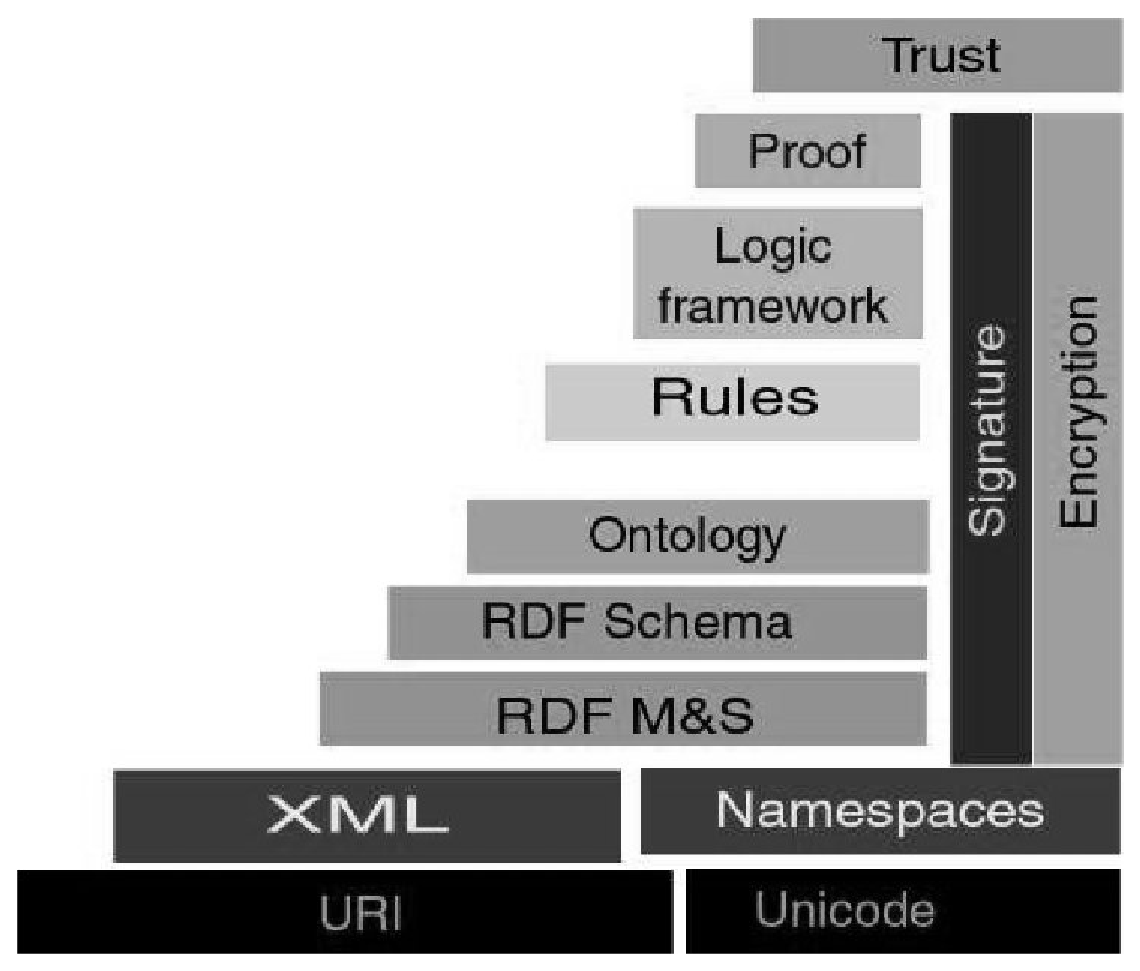
\includegraphics[width=10cm]{images/sw-stack-2002}
\caption{Arquitectura Web Semántica 2002.}
\label{fig:stack-2002}
\end{figure}

A continuación se explica someramente la intención de cada una de las capas y el por qué
de su presencia:
\begin{description}
\item[\gls{URI}/\gls{IRI}-Unicode.] Para dar un soporte estándar a una tecnología existen
dos factores fundamentales: nombrado e identificación única de cada uno de los
recursos y codificación de los mismos. Por esta doble razón aparecen los \textit{Unified
Resource Identifier}y la codificación estándar Unicode, implementada principalmente en UTF-8.
\begin{example}
URI: protocolo:dirección:directorio:recurso, \url{http://www.josemalvarez.es/foaf.rdf}
\end{example}

\item[\gls{XML}~\cite{XML11}.] lenguaje extensible de marcas (\textit{eXtensible Markup
Language}) es un formato estándar creado para la estructuración de datos.
Hoy en día se encuentra regulado por el \gls{W3C} que es el encargado de realizar las distintas
especificaciones y versiones desde Febrero de 1998. XML está basado en \gls{SGML}
(\textit{Standard Generalized Markup Language}, ISO 8879) que ya había sido establecido
en 1986. El uso principal de XML es la estructuración de datos, pero en general es utilizado por todas
aquellas aplicaciones informáticas en las cuales se pueda representar la información jerárquicamente.
El lenguaje XML es en sí mismo un metalenguaje utilizado ampliamente para definir otros
lenguajes. Consta entre otros, de elementos y atributos. Su orden y jerarquía
son los encargados de formar el lenguaje que definimos con XML. No se dispone de etiquetas predefinidas, como podría ser \gls{HTML}, esto
se deja a labor del usuario que es el encargado de definir un conjunto de elementos con sus
etiquetas asociadas, la semántica de los documentos es proporcionada por la aplicación que use
esos datos. Para definir la estructura de un documento XML, es decir, una 
gramática que indique el orden de los elementos y su jerarquía, lo podemos conseguir de
dos formas utilizando: 1) \gls{DTD} o 2) \gls{XML Schema}~\cite{XMLSchema}.

Es importante resaltar que un documento bien formado no es lo mismo que un documento
válido, un documento estará bien formado cuando siga las reglas sintácticas de
formato XML, mientras que un documento será válido si todos sus elementos están en orden correcto de anidación y está bien formado. Algunas de las razones 
por las que es interesante utilizar XML son las siguientes:
\begin{itemize}
\item Estándar para el intercambio de datos.
\item Facilidad de uso.
\item Legibilidad.
\item Implantación.
\item Extensibilidad.
\item Separación entre formato y contenido.
\item Tratamiento multiplataforma.
\item Es libre, especificaciones disponibles. 
\end{itemize}

\begin{figure}[!htbp]
\centering
\lstinputlisting[language=XML]{examples/events.xml}
\caption{Ejemplo de fichero XML.}
\label{fig:ejemplo-xml}
\end{figure}

Como aplicación práctica de XML, ver Figura~\ref{fig:ejemplo-xml}, y debido a la necesidad de tratamiento
automático para diferentes fines (formatos de presentación, transformación de un
vocabulario a otro, etc.) hay que destacar \gls{XSL}~\cite{XSL} generación del
contenido a partir de un documento XML de una manera rápida, sencilla y eficaz, cuyo objetivo principal es presentar al usuario final un 
interfaz del documento más entendible con el que pueda realizar un tratamiento de la información contenida en él de una manera más
asequible, sin necesidad de conocer el formato XML.

\begin{figure}[!htbp]
\centering
	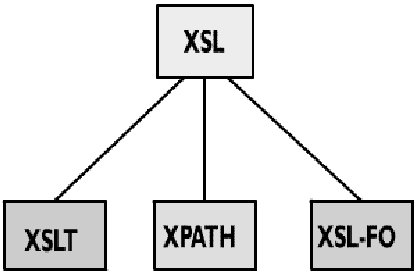
\includegraphics[width=6cm]{images/xsl}
\caption{Componentes de XSL.}
\label{fig:xsl}
\end{figure}

Por ello desde el consorcio \gls{W3C} se optó por realizar la especificación XSL con
el objetivo de presentar un modelo para el procesamiento de la información
almacenada en formato XML. La especificación redactada por el consorcio web para la transformación del contenido XML
se denomina XSL, se encarga de definir una hoja de estilo con la cual se transforma el fichero
XML en otro formato, teniendo en cuenta que la información en XML se almacena de forma
jerarquizada, con la definición de XSL se pretende poder presentar al usuario dicha información
en otros formatos estructurados como pueden ser: HTML, \gls{PDF}, etc., XSL es una especificación, pero 
el lenguaje del que hace uso para la realización de la transformación es XSLT con sintaxis de XPath~\cite{XPath}.

En \gls{XSLT} se define cómo se ha de realizar la transformación del documento XML y no
cuándo se debe realizar, la transformación del documento se realiza en distintos
pasos: 
\begin{itemize}
    \item Generación de un árbol a partir del fichero fuente de XML, esto se
    realiza mediante un procesador que analiza el documento, realizando al mismo tiempo una validación sintáctica del
mismo.
\item Procesamiento del árbol generado construyendo un nuevo árbol con la
información procesada, el recorrido del árbol generado se realiza en preorden, con la posibilidad de variar el tipo de recorrido, es importante tener en cuenta
el orden de evaluación de los nodos del árbol para así poder aplicar las
plantillas correctamente. 
\end{itemize}

El principal uso de XSLT como ha quedado patente en la introducción, es la transformación
de documentos XML para generar contenido web, lógicamente esto no aportaría demasiada potencia
a este lenguaje si solo sirviera para generar contenido web estático. En cambio usando
este lenguaje se genera contenido dinámico aplicando distintas reglas, como ejemplo se
podría obtener de una base de datos un fichero XML y con dicho fichero y una transformación
apropiada generar una página dinámica con contenidos auto-actualizables cada cierto tiempo, otro 
ejemplo de aplicación podría ser la conversión de un programa escrito en un lenguaje a otro, definiendo las reglas correctas. 
XSLT utiliza también \gls{XPath}, ver Figura~\ref{fig:xsl-example}, que es una especificación
para el acceso a los valores de los distintos nodos del árbol generados a partir del procesamiento
del fichero XML. 

\begin{figure}[!hbp]
\centering
\lstinputlisting[language=XML]{examples/events.xsl}
\caption{Ejemplo de hoja de estilo XSL.}
\label{fig:xsl-example}
\end{figure}


\item[\gls{XML Schema}~\cite{XMLSchema}.] En primer lugar es interesante diferenciar las dos
tecnologías establecidas para la definición de la estructura de un documento
XML: \begin{inparaenum}
     \item \textit{Document Type Definition} (\gls{DTD}) es un vocabulario para definir las
     reglas de construcción de un documento XML.     
     \item XML Schema: Vocabulario XML utilizado para definir otros vocabularios
     XML.  
     \end{inparaenum}

El incremento en el uso de \gls{XML} hace necesario la utilización de tecnología para poder
expresar la estructura del documento y así proceder a su validación. Aunque en principio el objetivo de ambos es el mismo: 
definir vocabularios XML para poder validarlos sintácticamente e imponer distintos tipos de 
restricciones como de cardinalidad o integridad, cada uno presenta unas características diferentes 
lo que supone que escoger entre uno u otro implique realizar un estudio de lo que se pretende desarrollar.
También disponemos de herramientas que nos permiten realizar la transformación de uno a
otro pero sólo en el sentido de DTD a XML Schema. Se puede pensar que XML Schema es el
sucesor de las DTD.

La utilización de XML Schema, ver Figura~\ref{fig:xsd-example}, se apoya en diferentes características que hacen
que su uso sea interesante en el ámbito de la Web Semántica:
\begin{itemize}
\item Espacios de nombres, permite utilizar los mismos identificadores en el
mismo documento, evitando así la ambigüedad.
\item Esquema, es la estructura que va a presentar el vocabulario XML construido, con
sus distintos elementos y atributos así como con las validaciones que sean
necesarias.
\item Documento instancia,  documento XML creado con una estructura
definida en un XML Schema y contra el cual se ``valida''.
\end{itemize}

Las razones que pueden llevar a elegir XML Schema son, entre otras, las siguientes:
\begin{itemize}
  \item Utiliza sintaxis XML.
  \item Perfectamente documentado.
  \item Define los elementos y atributos que pueden aparecer en un documento instancia.
  \item Establece la jerarquía y orden de los distintos elementos.
  \item Podemos crear distintos tipos genéricos.
  \item Extensible.
  \item Inclusión de documentos externos.
  \item Expresividad.
  \item Posibilidad de documentación.
  \item Tipos de datos simples, complejos, derivados.
  \item Expresión de restricciones de integridad y cardinalidad.
  \item Reutilización de tipos por extensión o restricción.
  \item \ldots  
\end{itemize}


\begin{figure}[!htbp]
\centering
\lstinputlisting[language=XML]{examples/events.xsd}
\caption{Ejemplo de XML Schema.}
\label{fig:xsd-example}
\end{figure}


La utilización de XML Schema es crítica en los servicios web basados en \gls{WSDL}~\cite{WSDL20} y \gls{SOAP}~\cite{SOAP11} y 
está muy asentada en entornos de desarrollo basados en Java a través de herramientas como \gls{JAXB}.

\item[\gls{RDF}~\cite{RDF}.] \textit{Resource Description Framework}, se encarga
de describir los recursos, añadiéndoles la metainformación necesaria en
un formato procesable. En la siguiente Sección~\ref{rdf} abordaremos la descripción de
RDF de manera más extensa.

\item[Ontologías:] Los documentos etiquetados constituyen una gran cantidad
de información disponible para utilizar por la máquina. Están disponibles los datos, pero
todavía no hay capacidad semántica. Es necesario construir un modelo donde ``encajar''
esos datos. Para añadir la componente semántica mediante ontologías, ver Sección
\ref{ontologias}, se pueden utilizar diferentes lenguajes, cuyo estudio se 
abordará en la Sección~\ref{lenguajes}.

\item[Capas superiores:] La arquitectura propone diferentes niveles en los
que se colocan las reglas y la lógica, debido a su complejidad todavía es precipitado definirlas por completo y las discusiones se mantienen
abiertas en grupos de trabajo del \gls{W3C} como el \gls{RIF}~\cite{rif-core}. 
Los módulos transversales de ``firma''~\cite{XML-dsig} y 
``encriptación''~\cite{XML-enc} están definidos y se
pueden encontrar como recomendaciones del W3C.

\end{description}

Aunque las ventajas de un diseño basado en capas está sobradamente demostrado en
bibliografía de ingeniería del \textit{software}, hay que resaltar que esta primera
aproximación ha sido modificada con el objetivo de recoger la realidad de la
arquitectura para la Web Semántica. Hay que tener en cuenta que la primera
versión propuesta por \textit{Tim Berners Lee} (web XML) ofrecía una visión ideal
que contemplaba todas las partes implicadas, pero que no tenía el efecto experiencia
de la construcción de aplicaciones y de los posibles problemas que se podrían
encontrar. Por ello, esta arquitectura ha sido rediseñada planteando un modelo
más cercano a la realidad, por lo menos de las aplicaciones y problemas, y que
también es conocida como las ``dos torres''~\cite{kifer05} (web RDF), ver Figura~\ref{fig:stack-2005}.

\begin{figure}[!htbp]
\centering
	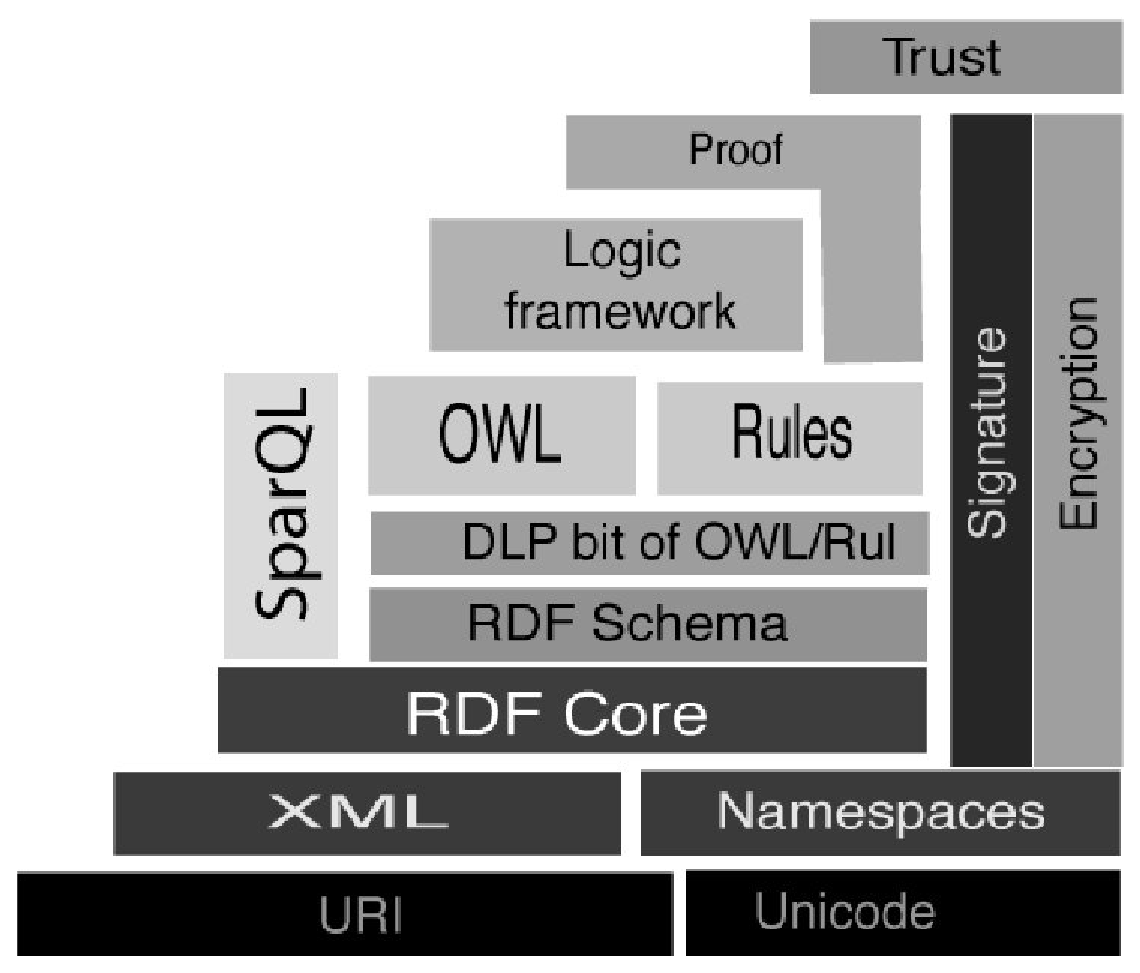
\includegraphics[width=10cm]{images/sw-stack-2005}
\caption{Arquitectura Web Semántica 2005.}
\label{fig:stack-2005}
\end{figure}

La propuesta de cambio surge porque la Lógica Descriptiva, que utiliza \gls{OWL}, no
tiene un poder expresivo suficiente para solucionar el problema de la
representación de conocimiento y razonamiento en la Web Semántica. OWL no puede
tratar con información de una forma dinámica, no tiene predicados \textit{n-arios}, no
soporta símbolos de función, etc. De ahí que se valorará la posibilidad de extender las bases
de conocimiento en OWL con reglas para aumentar la expresividad de los modelos y
ganar en capacidad de inferencia.

Las reglas, en programación lógica como PROLOG, tienen una larga tradición en
las ciencias de la computación y se llevan estudiando desde hace más de 20 años. Sin
embargo, la extensión de OWL con reglas no es una tarea sencilla. En general, las reglas 
están basadas también en un subconjunto de la lógica de primer orden, la
lógica \textit{Horn}, aunque su semántica formal es diferente, no está basada en teoría de modelos. La diferencia fundamental, aparte del tratamiento
de la negación y cuestiones de expresividad, tiene que ver con OWL, ya que, 
debido a su semántica de primer orden, utiliza la hipótesis de mundo abierto,
mientras que las reglas habituales de programación lógica utilizan mundo cerrado. 

La extensión más conocida de OWL en este sentido es \gls{SWRL}~\cite{Swrl}, que permite cláusulas
Horn como axiomas en las bases de conocimiento en OWL. Este lenguaje mantiene
el mundo abierto de OWL, pero penaliza en rendimiento debido a su alto coste computacional.

Debido a esta serie de problemas, se ha sugerido la opción de separar ontologías y
reglas (lógica descriptiva y programación lógica) y utilizar cada tecnología en casos
de uso pertinentes y apropiados. La combinación entre ambos, un objetivo verdaderamente ambicioso de la Web Semántica, 
ya no sería mediante la extensión de OWL con algún tipo de formalismo para la expresión de reglas, sino mediante la construcción
de un interfaz lógico que permita desde las reglas utilizar información definida
en las ontologías, y desde éstas, información inferida por el
comportamiento de los sistemas de reglas.

Destacar la aparición del lenguaje de consulta para RDF, \gls{SPARQL}~\cite{Sparql} y su última
versión SPARQL 1.1, creado por la necesidad de disponer de un lenguaje de acceso a los recursos
definidos en forma de grafo y con una semántica definida~\cite{Perez:2009:SCS:1567274.1567278}. El modelo semántico~\cite{citeulike:1556975} 
proporcionado por RDF permite tratar cualquier recurso como una entidad con descripción asociada. No obstante, el uso de RDF no es
suficiente para la elaboración de modelos de dominio más ricos y descriptivos, razón por la cual surge un lenguaje como OWL que apoyado sobre el modelo de RDF
permite realizar formalizaciones utilizando diferentes lógicas (principalmente \textit{Description Logics}).

\subsubsection{Lenguajes para la Web Semántica: Creando ontologías}\label{lenguajes}
La construcción de una base de conocimiento~\cite{GruberOnto} utilizando ontologías puede
realizarse con distintos lenguajes y diferentes grados de expresividad lógica~\cite{HoPa10a,Kifer:1989:FHL:66926.66939}.
La selección de la lógica apropiada para la modelización de nuestra base de
conocimiento no es una cuestión sencilla y debemos contemplar diferentes
factores: grado de computabilidad, decidibilidad, soporte razonadores, etc.
Todos ellos determinarán la lógica a utilizar ya que no se puede señalar arbitrariamente que se debe utilizar un nivel lógico cuando no es necesario para
el modelo formal.
\subsubsection{RDF}\label{rdf}
El primer lenguaje que nos encontramos para la creación de ontologías es \gls{RDF}
(\textit{Resource Description Framework}) como soporte básico a la par que potente, 
para añadir semántica a los recursos (documentos entre otros). La primera observación 
a realizar es la distinción entre: \begin{inparaenum}\item Modelo de datos, basado en
tripletas Sujeto-Predicado-Objeto. \item Formato de datos, puede utilizar RDF/XML (normativo)
como formato para la serialización del modelo.\end{inparaenum}

El modelo de datos de RDF utiliza tripletas, ver Figura~\ref{fig:rdf-model}, encargadas de describir recursos:
\begin{description}
\item[Sujeto:] recurso sobre el que vamos a realizar una afirmación. Están
identificados de forma única a través de URIs. Por ejemplo: Yo.
\item[Predicado:] es la afirmación sobre el sujeto. Por ejemplo: ``tengoNombre''.
\item[Objeto:] valor del predicado para este sujeto. Por ejemplo: ``Jose
María''@es.
\end{description}

\begin{figure}[!htbp]
\centering
	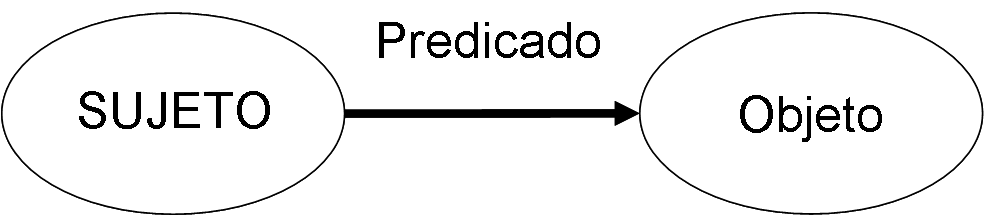
\includegraphics[width=10cm]{images/rdf-model}
\caption{Modelo de tripletas RDF.}
\label{fig:rdf-model}
\end{figure}

Usando RDF pueden realizarse afirmaciones simples sobre ``cosas'': ``Este
documento de memoria tiene de creador'' a ``Jose María Alvarez'' puede expresarse en
RDF usando la tripleta (memoria, ``tieneCreador'', ``Jose María Alvarez''). 
A su vez  se pueden generar nuevas tripletas (memoria, ``tieneFecha'',
``Enero 2012'') o (memoria, ``tieneFormato'', ``PDF''), generando así un
modelo semántico simple pero perfectamente válido. Si se le añade el uso de colecciones y 
la capacidad de ``reificación'' (afirmaciones sobre otras
afirmaciones) se conseguirá una capacidad de expresión muy potente asentada en un
sencillo lenguaje. En cuanto, a la serialización de RDF o su formato, existen diferentes estándar
perfectamente válidos para su tratamiento automático por las máquinas y más o
menos amigables para los humanos. 
\begin{itemize}
  \item \gls{RDF/XML}~\cite{rdf-syntax} formato estándar y normativo por excelencia, ver Figura~\ref{fig:rdf-n3}. 
\begin{figure}[!htbp]
\centering
  \begin{lstlisting} 
<rdf:RDF xmlns:rdf="http://www.w3.org/1999/02/22-rdf-syntax-ns#"
  xmlns:rdfs="http://www.w3.org/2000/01/rdf-schema#"
  xmlns:dc="http://purl.org/dc/elements/1.1/">
    <rdf:Description rdf:about="http://petra.euitio.uniovi.es/~i1637566/">
      <dc:creator>Jose M. Alvarez</dc:creator>
    </rdf:Description>
</rdf:RDF>  
  \end{lstlisting} 
\caption{Ejemplo de tripletas de RDF en RDF/XML.}
\label{fig:rdf-n3}
\end{figure}  

\item Otros como: \gls{RDFa}~\cite{rdfa-primer}, \gls{Turtle}~\cite{turtle-syntax}, \gls{N3}~\cite{n3-syntax} ,\gls{RDF}/\gls{JSON}~\cite{rdf-json} o RDF binario~\cite{rdf-binario}.   
\begin{figure}[!htbp]
\centering
  \begin{lstlisting} 
@prefix dc <http://http://purl.org/dc/elements/1.1/>
<http://petra.euitio.uniovi.es/~i1637566/> dc:creator "Jose M. Alvarez"
  \end{lstlisting}
\caption{Ejemplo de tripleta de RDF en N3.}
\label{fig:rdf-n3}
\end{figure}


 \end{itemize}

En definitiva, RDF provee un mecanismo muy útil para describir recursos que
no realiza presunciones sobre un dominio y capaz de representar a cualquiera
de ellos. La declaración de propiedades (atributos) y su valor semántico se definen
en el contexto de RDF con RDFS (\textit{\gls{RDF Schema}}). RDFS se construye por
encima de RDF y sirve, no solo para definir las propiedades del recurso, sino también
el tipo de recurso. Se pueden crear \textit{clases de recursos}, restringir
combinaciones de las clases, de las relaciones, además de ser el primer nivel de
semántica que permite detectar estas aserciones. RDFS está basado en el
metamodelado de objetos, el principal problema lo constituye la posibilidad de que una
misma clase pueda desarrollar un doble rol de clase o de instancia. Aunque se puede utilizar como
un lenguaje de ontologías desde el punto de vista del manejo de clases, propiedades, rangos y dominios sobre propiedades. 
La posibilidad de generación de jerarquía de conceptos es un lenguaje muy limitado para la expresión de datos en
detalles y no asegura la computabilidad. Es interesante conocer algunos de los vocabularios RDF, especialmente
con el advenimiento de la iniciativa de \linkeddata, que se han creado con distinto propósito, con muy buena 
acogida en la comunidad de Internet y cada día con un uso más extendido: 

\begin{description}
\item[\textit{Dublin Core}.] Vocabulario RDF con las propiedades más comunes y semántica bien definida para el etiquetado de cualquier documento.

\begin{itemize}
  \item Cada etiqueta es opcional y puede estar repetida. Un documento no
  necesita tener resumen y puede tener varios autores.
  \item La mayoría de etiquetas tienen cualificadores para refinar (nunca extender) su significado.
Por ejemplo, la etiqueta ``fecha'' tendrá como cualificadores ``de publicación'',
``de creación'', etc.
\item Principio del Uno-a-Uno. Los metadatos se refieren a un documento
concreto, no a lo representado. 
\item  Principio del \textit{Dumb-down}: Si no se procesan las restricciones al
significado de las propiedades, estas deben seguir proporcionando información
útil. Se pierde nivel de detalle, pero la información sigue siendo válida.
\item Las buenas prácticas de uso para una etiqueta determinada pueden variar por
el contexto. El creador no puede dar por supuesto que serán interpretadas exclusivamente por
una máquina. Esto impondrá algunas restricciones a como se construyen los
metadatos, pero no se debe eludir que el requisito fundamental de
estos es su utilidad para descubrir información.
\end{itemize}

Usando estos principios, \textit{Dublin Core} se impuso el objetivo de lograr un lenguaje
de etiquetado: simple y fácil de mantener, semántica esencial y de significado común, alcance internacional y extensible.
Podemos establecer dos escenarios muy habituales en el uso de este vocabulario:
\begin{enumerate}
  \item En los metaelementos presentes en \gls{HTML} y \gls{XHTML}, ver Figura~\ref{fig:html-dc-example}.

\begin{figure}[!htbp]
\centering
  \begin{lstlisting} 
  <head>
<title>Dublin Core Metadata Initiative (DCMI)</title>
<link rel="schema.DC" href="http://purl.org/dc/elements/1.1/" />
<meta name="DC.title" content="Dublin Core Metadata Initiative (DCMI) Home Page" />
<meta name="DC.description" content="The Dublin Core Metadata Initiative is an open forum . . . metadata standards and practices." />
<meta name="DC.date" content="2011-10-01" />
<meta name="DC.format" content="text/html" />
<meta name="DC.contributor" content="Dublin Core Metadata Initiative" />
<meta name="DC.language" content="en" />
</head>  
 \end{lstlisting} 
\label{fig:html-dc-example}
\caption{Ejemplo de \textit{Dublin Core} en HTML/XHTML.}
\end{figure}
 
\item En documentos RDF propiamente dichos como metadatos de los recursos. A
continuación, se puede ver en la Figura~\ref{fig:rdf-dc-example} el uso de \textit{Dublin Core} en combinación con \gls{RSS}.

\begin{figure}[!htbp]
\centering
\begin{lstlisting}
<rdf:RDF
 xmlns:rdf="http://www.w3.org/1999/02/22-rdf-syntax-ns#"
 xmlns="http://purl.org/rss/1.0/"
 xmlns:dc="http://purl.org/dc/elements/1.1/"
 xmlns:syn="http://purl.org/rss/1.0/modules/syndication/"
 xmlns:taxo="http://purl.org/rss/1.0/modules/taxonomy/"
>
<channel rdf:about="http://dublincore.org">
<title>Dublin Core Metadata Initiative</title>
<link>http://dublincore.org/</link>
<description>Making it easier to find information.</description>
<dc:language>en-us</dc:language>
<dc:rights>1995-2007</dc:rights>
<dc:date>2007-10-01</dc:date>
<items>
<rdf:Seq>
  <rdf:li rdf:resource="http://dublincore.org/news/2007/#dcmi-news-20071001-01" />
  <rdf:li rdf:resource="http://dublincore.org/news/2007/#dcmi-news-20071001-02" />
  <rdf:li rdf:resource="http://dublincore.org/news/2007/#dcmi-news-20071001-03" />
  <rdf:li rdf:resource="http://dublincore.org/news/2007/#dcmi-news-20071001-04" />
</rdf:Seq>
</items>
</channel>

</rdf:RDF>
 \end{lstlisting} 
\label{fig:rdf-dc-example}
\caption{Ejemplo de \textit{Dublin Core} con RDF.}
\end{figure}

\end{enumerate}

\item[\gls{SKOS}-Core~\cite{SKOS-Core}.] Vocabulario RDF utilizado para la representación de conocimiento 
de forma simple a través de conceptos, para ser procesado por máquinas de forma
automática: vocabularios controlados, taxonomías, tesauros, esquemas
conceptuales, glosarios o esquemas categorizados. Algunas de las propiedades de SKOS que 
confieren interés este vocabulario:
\begin{itemize}
\item Identificación de conceptos a través de URIs.
\item  Etiquetado de conceptos: \textit{prefLabel}, \textit{altLabel},
\textit{prefSymbol}, \textit{altSymbol}, etc.
\item Descripción y documentación (conceptos): \textit{definition}, \textit{example}, \textit{scopeNote},
\textit{version}, \textit{changeNote}, etc.
\item Relaciones entre conceptos: \textit{broader}, \textit{narrower},
\textit{related}, etc. 
\item Indexación: \textit{subject}.
\item Soporte multiling\"{u}e
\end{itemize}

En la siguiente Figura~\ref{fig:skos} se presenta un ejemplo más completo del
uso de SKOS-Core para la descripción de conceptos:
 
\begin{figure}[!htbp]
\centering
	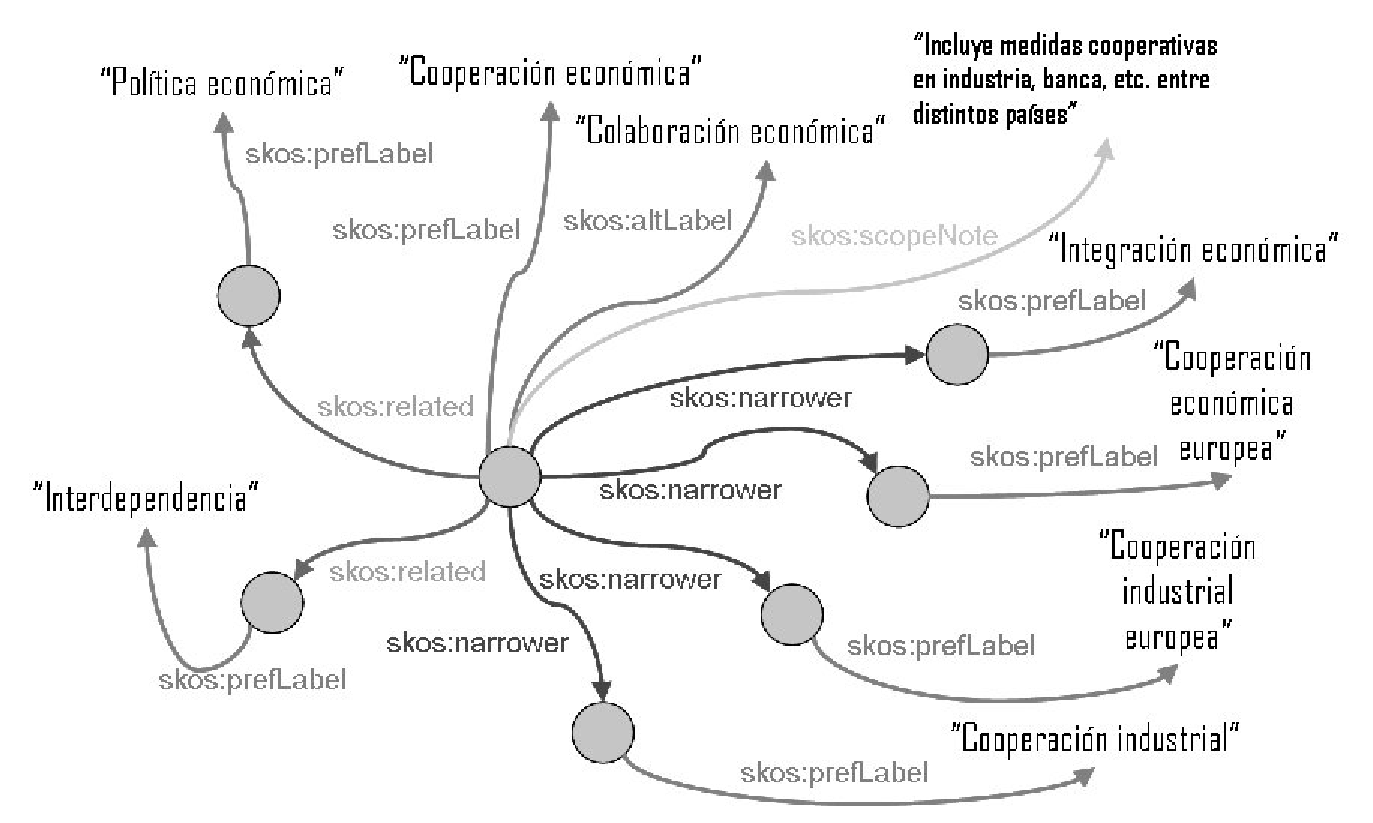
\includegraphics[width=14cm]{images/skos}
\caption{Concepto expresado en SKOS-Core.}
\label{fig:skos}
\end{figure}

Debe puntualizarse que el uso de SKOS-Core está siendo objeto de estudio para la
representación de recursos lexicográficos~\cite{Milin} desde un punto de vista de la
lingüística y como un avance tecnológico en este campo.

\item[\gls{FOAF} y \gls{DOAP}.] Vocabularios RDF para definir personas y amistades (\textit{Friend Of A Friend}), ver Figura~\ref{fig:foaf-example}, o 
proyectos (\textit{Description Of A Project}), 
ver Figura~\ref{fig:doap-example}. Cada vez hay un mayor interés por este tipo de tecnologías y algunos proyectos de gran envergadura como 
Apache o RDF Ohloh~\cite{Ferndez08rdfohloh}, que incluyen muchos subproyectos, programas, etc., utilizan estas
descripciones semánticas para cada módulo.

\begin{figure}[!htbp]
\centering
  \begin{lstlisting}
<#me> a foaf:Person;
	foaf:family_name "Alvarez Rodr\u00EDguez";
	foaf:givenname "Jose Mar\u00EDa";
	foaf:homepage <http://josemalvarez.es>;
	foaf:knows _:bnode2016979200;
	foaf:mbox_sha1sum "0d1d9ad2de64fd900d03c18e3d2608171832d155";
	foaf:name "Jose Mar\u00EDa Alvarez Rodr\u00EDguez";
	foaf:nick "chema";
	foaf:phone <tel:+34-666-714-721>;
	foaf:schoolHomepage <http://www.uniovi.es/inicio/>;
	foaf:title "Sr.";
	foaf:workplaceHomepage <http://www.weso.es>.
_:bnode2016979200 a foaf:Person;
	rdfs:seeAlso <http://www.di.uniovi.es/~labra/labraFoaf.rdf>;
	foaf:mbox_sha1sum "5fa5d69bac0c1396825c475ec19325ec0ffd5569";
	foaf:name "Jose Emilio Labra".
  \end{lstlisting}
\caption{Ejemplo parcial de documento FOAF en N3.}
\label{fig:foaf-example}
\end{figure}


\begin{figure}[!htbp]
\centering
  \begin{lstlisting}
<http://rdfohloh.wikier.org/project/moldeas/rdf> 
	dct:isFormatOf 	<http://rdfohloh.wikier.org/project/moldeas>;
	a foaf:Document;
	rdfs:label "MOLDEAS's DOAP document serialized in RDF/XML";
	foaf:primaryTopic <http://rdfohloh.wikier.org/project/moldeas>.
	<http://rdfohloh.wikier.org/project/moldeas> dct:updated "2012-01-22T13:02:25Z";
	rdfohloh:ohloh-page <http://www.ohloh.net/projects/moldeas>;
	doap:created "2011-10-14T09:19:11Z";
	doap:description "This work aims to apply the semantic web and 
	    LOD approaches to public procurement notices...";
	doap:download-page <http://code.google.com/p/moldeas/downloads/list>;
	doap:homepage <http://purl.org/weso/moldeas/>;
	doap:name "MOLDEAS";
	doap:programming-language "JavaScript";
	a doap:Project;
	= <http://rdfohloh.wikier.org/project/586667>;
	skos:subject <http://dbpedia.org/resource/Java>, 
	<http://dbpedia.org/resource/JavaScript>.
  \end{lstlisting}
\caption{Ejemplo parcial de documento DOAP en N3.}
\label{fig:doap-example}
\end{figure}

\item[\gls{SIOC}.] (\textit{Semantically-Interlinked Online Communities}). Es una ontología desarrollada 
por el equipo de Web Semántica de DERI Galway para describir semánticamente
distintas comunidades \textit{online}. SIOC integra, ver Figuras~\ref{fig:sioc} y~\ref{fig:sioc-example}, distintos vocabularios RDF con el
objetivo de reutilizar las definiciones ya realizadas en \gls{FOAF}, \gls{SKOS},
\gls{RSS} o \textit{Dublin Core}. Se ha empleado con éxito en distintas aplicaciones para gestionar y
describir toda la información disponible de las comunidades \textit{online}: listas de correo (SWAML~\cite{Sergio}), 
foros, etc.
 
\begin{figure}[!htb]
\centering
	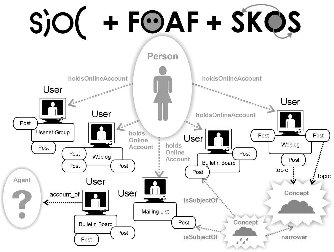
\includegraphics[width=12cm]{images/sioc}
\caption{SIOC integración con otros vocabularios.}
\label{fig:sioc}
\end{figure}

\begin{figure}[!htbp]
\centering
  \begin{lstlisting}
<rdf:RDF
  xmlns:sioc='http://rdfs.org/sioc/ns#'
  xmlns:rdf='http://www.w3.org/1999/02/22-rdf-syntax-ns#'
  xmlns:dc='http://purl.org/dc/elements/1.1/'
  xmlns:mvcb='http://webns.net/mvcb/'
>
  <sioc:Site rdf:about="http://groups.google.com/group/sioc-dev">
    <sioc:host_of>
      <sioc:Forum rdf:about="http://swaml.berlios.de/demos/sioc-dev/index.rdf#SIOC-Dev">
        <dc:description>SIOC development mailing list</dc:description>
        <mvcb:errorReportsTo rdf:resource="http://swaml.berlios.de/bugs"/>
        <sioc:container_of rdf:resource="http://swaml.berlios.de/demos/sioc-dev/2006-Dec/post-419.rdf"/>
        <dc:date>2007-06-18</dc:date>
        <dc:title>SIOC-Dev</dc:title>
        <mvcb:generatorAgent rdf:resource="http://swaml.berlios.de/doap.rdf"/>
        <sioc:has_host rdf:resource="http://groups.google.com/group/sioc-dev"/>
        <sioc:has_subscriber rdf:resource="http://swaml.berlios.de/demos/sioc-dev/subscribers.rdf#s26"/>
      </sioc:Forum>
    </sioc:host_of>
  </sioc:Site>
</rdf:RDF>
  \end{lstlisting}
\caption{Ejemplo de descripción con SIOC.}
\label{fig:sioc-example}
\end{figure}

\item[\gls{RSS}.] Existen diferentes versiones y definiciones de este vocabulario RDF, ver Figura~\ref{fig:rss-example}: \textit{Rich Site Summary} (RSS 0.91), XML; 
\textit{RDF Site Summary} (RSS 0.9 y 1.0), RDF; \textit{Really Simple Syndication} (RSS 2.0). La definición
realizada en el \gls{W3C} es la siguiente:

\begin{Frame}
Vocabulario RDF basado en XML que permite la catalogación de información (noticias y eventos) 
de los usuarios. Los archivos RSS contienen metadatos sobre fuentes de información especificadas 
por los usuarios, cuya función principal es notificar de forma automática cualquier cambio que se realice 
en esos recursos de interés.
\end{Frame}

\begin{figure}[!htb]
\centering
\lstinputlisting[language=XML]{examples/rss.rss}
\label{fig:rss-example}
\caption{Ejemplo de canal RSS.}
\end{figure}

\end{description}

En resumen, se dispone de un lenguaje muy útil y sencillo para describir recursos (RDF) y 
un esfuerzo en forma de vocabulario para la definición de recursos más detallada (RDFS) pero incompleto. 
Por ello, a continuación, se expondrán algunos de los lenguajes más completos que han surgido para 
intentar mejorar los puntos débiles de esta primera aproximación para la expresión de modelos semánticos. En cuanto
a vocabularios RDF existen una infinidad~\cite{common-vocabularies} de ellos para ser utilizados en distintos contextos que han sido
enormemente impulsados por la corriente \linkeddata y \opendata.
%Avoiding too many floats 
\clearpage

\subsubsection{OIL}
El \textit{Ontology Inference Layer}~\cite{Fensel01oil:an} (\gls{OIL}) desarrollado en el proyecto Europeo 
\textit{OntoKnowledge} está construido por encima de \gls{RDF} y RDFS utilizando muchos de sus constructores e intentando
mantener la compatibilidad hacia atrás. OIL provee características de modelado
basada en lógica de marcos~\cite{Kifer:1989:FHL:66926.66939} y \textit{Description Logic}~\cite{baader03description}.

La importancia de OIL reside en la unificación de:
\begin{itemize}
\item \textit{Description Logic}, heredando su semántica formal y la capacidad
de razonamiento efectivo (FaCT++, Racer o Pellet).
\item Sistemas basados en marcos, incorpora las características básicas de
modelado basado en marcos (conceptos, superclases, atributos, etc.).
\item Estándares web, construido sobre RDF y RDFS y utilizando como formato de
intercambio de datos XML.
\end{itemize}

Las ontologías creadas con OIL distinguen distintos meta niveles, con el
objetivo de proporcionar distintos niveles de servicio que pueden ser válidos para un
gran número de ontologías y aplicaciones:
\begin{description}
\item[Primer meta nivel:] también conocido como \textit{definición de ontologías}, en la
cual se proveen las definiciones de ontología, terminología que debería ser
instanciada para definir un vocabulario estructurado con la semántica adecuada.
\item[Segundo meta nivel:] conocido como ``meta meta'' nivel o \textit{contenedor de
ontologías}, describe las características de la ontología tales como autor,
nombre, ámbito, etc. Las anotaciones de este nivel se hacen mediante
\textit{Dublin Core}.
\end{description}

La capacidad de razonamiento es otra de las características importantes de OIL, que no estaba presente en RDF. Habitualmente esta capacidad se utiliza
para realizar las operaciones de clasificación, validación de consistencia e inferencia de nuevo conocimiento de acuerdo a distintos 
niveles de expresividad: 

\begin{description}
\item[Core OIL:] prácticamente compatible con RDFS exceptuando la capacidad de
``reificación''.
\item[Standard OIL:] lenguaje que captura las primitivas y constructores necesarios para
construir modelos semánticos con capacidad de inferencia.
\item[Instance OIL:] inclusión de ``instancias''.
\item[Heavy OIL:] capacidades extras de representación y razonamiento.
\end{description}


\begin{figure}[htb]
\centering
	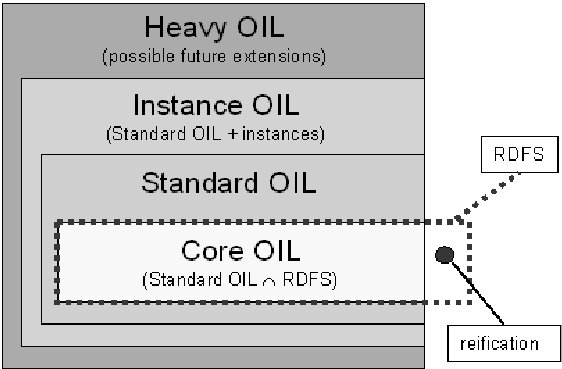
\includegraphics[width=10cm]{images/oil}
\caption{Niveles de expresividad OIL.}
\label{fig:oil}
\end{figure}

Cabe concluir, por tanto, que las principales ventajas de OIL se resumen en:
\begin{inparaenum} \item una aplicación no está obligada a trabajar con un
lenguaje más expresivo de lo necesario. \item aplicaciones que utilicen la
expresividad más baja pueden añadir aspectos de otras ontologías.
\item aplicaciones con un alto nivel de complejidad pueden utilizar
características de otras más simples.\end{inparaenum}

El trabajo realizado en OIL tiene su continuación en el siguiente lenguaje de
modelado de ontologías \gls{DAML+OIL}, ver Figura~\ref{daml+oil}, realizado por la cooperación
de iniciativas europeas y americanas.

\subsubsection{DAML+OIL}\label{daml+oil}
\gls{DAML+OIL}~\cite{HM00} es un lenguaje de marcado semántico para recursos web creado por la cooperación de las iniciativas
europeas (OIL) y americanas (DAML-ONT, \gls{DARPA} \textit{Agent Markup Language})
en el desarrollo de ontologías. El objetivo de desarrollo de este lenguaje está
especialmente centrado para la Web Semántica, modelización de dominios concretos,
utilizando los estándares (\gls{XML} y \gls{RDF}) y añadiendo una serie de primitivas de
orientación a objetos (clases, propiedades, axiomas y aserciones),
sistemas basados en marcos y parte de \textit{Description Logic}. Además, 
DAML+OIL da soporte a los tipos de datos de \gls{XML Schema}, separando las instancias
de una clase y de las instancias de tipos de datos. El significado de DAML+OIL
está definido por un modelo semántico estándar basado en las interpretaciones, consistiendo éstas 
en un dominio del discurso y una función de interpretación.

\subsubsection{OWL}\label{owl}
\gls{OWL}, lenguaje de ontologías para la web, sucesor de DAML+OIL, actualmente está
siendo desarrollado por el W3C, su primera versión estable es OWL 1.0, 
aunque que ya se ha publicado una nueva versión OWL 1.1~\cite{OWL11} y OWL2~\cite{owl2-primer}.

Como lenguaje para ontologías es una potente herramienta que dota de la
expresividad necesaria para mejorar algunos de los servicios más utilizados en
la red de Internet: búsqueda, manejo del conocimiento, interacción entre agentes
automáticos etc. Desde un punto de vista más formal, OWL está formado por
un conjunto de primitivas o constructores de metamodelado que son el punto de
partida para operaciones más complejas, como las de razonamiento. Actualmente,
aunque las características genéricas de OWL tienen su origen en OIL, se distinguen
al menos 3 versiones de OWL (en su versión 1.0 y 1.1) dependiendo de su expresividad, complejidad y grado
de computabilidad, cada versión superior de OWL contiene a la anterior
($Lite\subset DL \subset FULL$).

\begin{description}
\item[OWL-FULL.] Se pueden utilizar todos los constructores y primitivas
definidos en OWL y no restringe el uso de RDF. Esto implica que no se garantiza
su decidibilidad pero en cambio, como familia de \textit{Description Logics}
posee un gran poder expresivo: tratar clases como instancias, definir
propiedades sobre tipos de datos (\textit{string}, \textit{float}, etc.) .

\item[OWL-DL.] Subconjunto decidible de OWL-FULL, supone la máxima expresividad
computable. Cada modelo realizado en OWL-DL genera directamente un modelo
semántico en \textit{Description Logics}.

\item[OWL-Lite.] Añade restricciones adicionales sobre en el uso de los
constructores de OWL, básicamente se pueden modelar jerarquías con restricciones
sencillas.
\end{description}

Para advertir a que nivel de expresividad y complejidad se puede trabajar
dependiendo del lenguaje utilizado se dispone la Figura~\ref{fig:owl-dialects}, extraída del laboratorio OntoText.

\begin{figure}[htb]
\centering
	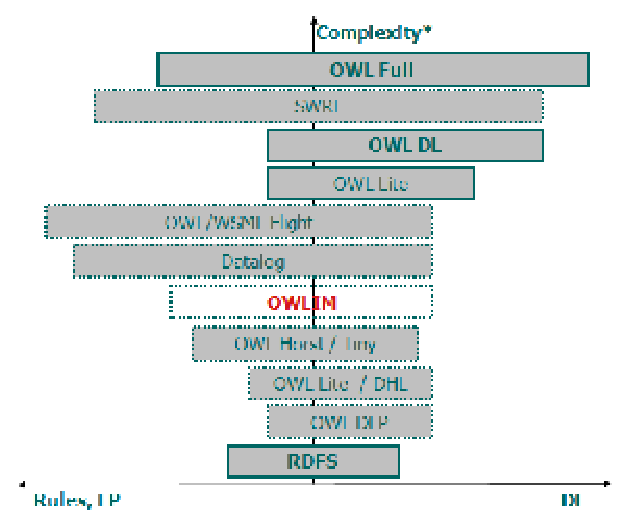
\includegraphics[width=10cm]{images/owl-dialects}
\caption{Algunos lenguajes para la Web Semántica por OntoText.}
\label{fig:owl-dialects}
\end{figure}


Algunas de las características que hacen interesante el uso de OWL en el ámbito
de la Web Semántica son:
\begin{itemize}
  \item Las ontologías en OWL son una serie de axiomas y hechos que pueden
  reutilizar otras ontologías (importándolas). Además, como documento que son
  (serializado en RDF/XML), están identificadas por un URI y tienen asociada cierta metainformación
  (author, dominio, fecha, etc.) que permite que sean referenciables como
  cualquier otro recurso en la red.
  \item Los axiomas son utilizados para asociar una serie de características
  (descripciones, restricciones, etc.) a las clases y propiedades de la
  ontología. 
\item Los hechos proporcionan información particular de una determinada instancia. 
\end{itemize}

Como ejemplo de utilización de OWL, en su versión DL y con características de OWL2, se presenta una sencilla
ontología, ver Figura~\ref{fig:psydiag}, que modela un sistema de diagnóstico psicológico con capacidad de clasificar individuos
de acuerdo a sus síntomas, ver Figura~\ref{fig:psydiag-axiomas}, con sintaxis Manchester.

\begin{figure}[htb]
\centering
	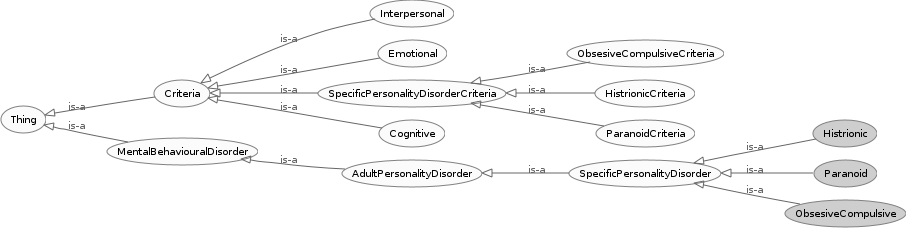
\includegraphics[width=16cm]{images/psydiag}
\caption{Ontología de ejemplo en OWL2 para diagnóstico psicológico.}
\label{fig:psydiag}
\end{figure}


\begin{figure}[htb]
\centering
 \begin{lstlisting} 
Class: <http://example.org/psydiag.owl/Histrionic>

    EquivalentTo: 
        <http://example.org/psydiag.owl/has-criteria> min 3
	      <http://example.org/psydiag.owl/HistrionicCriteria>,
        (not (<http://example.org/psydiag.owl/has-criteria> some 
	      <http://example.org/psydiag.owl/ObsesiveCompulsiveCriteria>))
         and (not (<http://example.org/psydiag.owl/has-criteria> some 
	      <http://example.org/psydiag.owl/ParanoidCriteria>))
         and (<http://example.org/psydiag.owl/has-criteria> only 
	      <http://example.org/psydiag.owl/HistrionicCriteria>)
    
    SubClassOf: 
        <http://example.org/psydiag.owl/SpecificPersonalityDisorder>

DisjointClasses: 
    <http://example.org/psydiag.owl/Histrionic>,
    <http://example.org/psydiag.owl/ObsesiveCompulsive>,
    <http://example.org/psydiag.owl/Paranoid>
  \end{lstlisting} 
\caption{Algunos axiomas de ejemplo en OWL2 para diagnóstico psicológico.}
\label{fig:psydiag-axiomas}
\end{figure}


\subsubsection{WSML}
\gls{WSML}~\cite{WSML2006} es la propuesta de lenguajes formales realizado en \gls{WSMO}~\cite{WSMODeri} 
(relevante por su relación con los Servicios Web Semánticos) para la construcción de ontologías y que recoge 
distintas variantes de lógica, ver Figura~\ref{fig:wsml-layering}. En general, teniendo en cuenta los
distintos tipos de lógica de acuerdo a su expresividad es posible obtener diferentes serializaciones
de los modelos realizados con distintos lenguajes \gls{OWL}, WSML, F-Logic, etc. Esta característica
es muy interesante para el uso de razonadores con distintos tipos de algoritmos y capacidades de
razonamiento, independientemente del lenguaje en el que se haya modelado el dominio.

\begin{figure}[htb]
\centering
	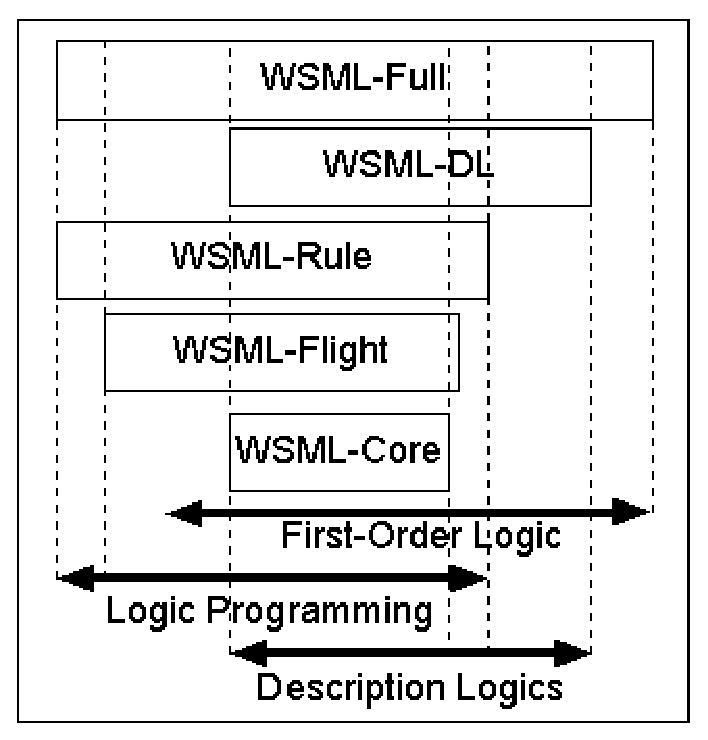
\includegraphics[width=8cm]{images/wsml-layering}
\caption{Capas de WSML.}
\label{fig:wsml-layering}
\end{figure}

\begin{note}
En OWL, con la arquitectura semántica de una torre, ver Figura~\ref{fig:stack-2002}, las
reglas ocuparían una capa por encima del lenguaje. Sin embargo, la práctica ha demostrado que la reglas son
parte de la ontología (no son condición necesaria, pero a un mínimo de complejidad en el
modelo se aprecia su utilidad). WSML incluye una variedad cubriendo esta
posibilidad (WSML-RULE).
\end{note}


\subsubsection{Nota}
Los lenguajes aquí presentados no son los únicos para la expresión de modelos de
conocimiento basados en semántica y reaprovechables para la web. No obstante,
al estar impulsados por el \gls{W3C} y pretender ser estándares, resultan de especial
interés y casi de conocimiento obligado para la comunidad de la Web Semántica.

No se puede determinar cuál es mejor que otro, la decisión de un lenguaje u otro
 debería venir asociado a un profundo análisis tanto funcional: propiedades  del
dominio a modelar y las necesidades lógicas del mismo como no funcional:
herramientas desarrollados, soporte, estabilidad, etc. Actualmente, \gls{OWL} 1.0
en su versión DL, \gls{WSML} y \gls{RDF} están siendo ampliamente utilizados mientras que las
propuestas de \gls{OIL}, \gls{DAML+OIL} y RDFS o bien están obsoletas o no han cumplido
las expectativas de los desarrolladores.


 
                                                           
\subsection{Ontolog\'ias}\label{ontologias}
\subsubsection{Antecedentes y Definición}
El desarrollo de las ontologías se deriva directamente de la filosofía, 
Aristóteles acuña el término ``Categoría'' como palabra para describir las
diferentes clases en las que se dividían las cosas del mundo. 
El término ``ontología'' es relativamente moderno (siglo XIX), proviene del griego
$Ontos$ (Ser) y $Logos$ (Palabra), se empezó a utilizar para diferenciar el
estudio de la Teoría de Categorías que se hacía en biología, de hecho, el trabajo de categorización surge en muchas áreas de la
ciencia (filosofía, biología, medicina, lingüística, etc.).

El cuerpo de un esquema de conocimiento, \textit{lo} que se puede representar, está basado en una
conceptualización: objetos, conceptos y otras entidades, que se asume existen en
un determinado dominio y que mantienen unas relaciones entre sí. 

\begin{Frame}
\textit{Una ontología es una especificación (explícita) de una conceptualización}~\cite{GruberOnto}. 
\end{Frame}

Las ontologías, por consiguiente, son sistemas basados en el conocimiento (\textit{\gls{SBC}}) que
sirven como modelo unificado en la representación del mismo, adquiriendo incluso
grado de ingeniería~\cite{isbn1846283965,Benjamins98ontological}. En muchos
casos, la Web Semántica y por extensión las ontologías se apoyan en la
reutilización de conocimiento compartido. Las definiciones realizadas para las ontologías son variadas y todas dejan claro
que sirven para modelar cierto dominio (conjunto de conceptos y relaciones):

\begin{itemize}
  \item Una ontología define los términos básicos y las relaciones establecidas en cierta área.
  \item Especificación explícita de una conceptualización.
  \item Especificación formal y explícita de una conceptualización compartida.
  \item Teoría lógica que provee de forma explícita y parcialmente una conceptualización.
  \item \ldots
\end{itemize}

En el artículo~\cite{Studer98knowledge} los autores agregan
expresividad realizando la siguiente descripción completa de ontología:
\begin{itemize}
  \item Conceptualización, modelo abstracto de algún fenómeno del mundo,
  proveniente de la identificación de los conceptos relevantes de dicho
  fenómeno. \item Explícita, conceptos y restricciones usados se definen
  explícitamente. \item Formal, capacidad de ser legible e interpretable por las
  máquinas.
  \item Compartida, captura conocimiento consensuado.
\end{itemize}

Es posible fusionar las definiciones anteriores en nueva descripción del término ontología:
\begin{definition}
Modelo conceptual organizado mediante una taxonomía que permite definir
relaciones entre conceptos, funciones, instancias (elementos) y axiomas en un determinado
dominio.
\end{definition}

Para completar la definición de ontología hay que tener en cuenta la
nomenclatura que habitualmente se utiliza para nombrar a las distintas entidades
posibles y que en algunos casos puede dar lugar a errores:

\begin{itemize}
  \item Clase, concepto, categoría o tipo.
  \item Instancia, individual.
  \item Entidad, objeto (clase o instancia).
  \item Propiedad, relación, slot, atributo, rol.
\end{itemize}

En la actualidad, la construcción de sistemas basados en conocimiento conlleva la
creación partiendo de cero de nuevas bases de conocimiento. La aspiración debería ser
utilizar componentes reutilizables~\cite{Gruber93towards}, de esta manera los desarrolladores deberían
crear sistemas con la agregación del conocimiento ya existente. El conocimiento definido, 
las técnicas de resolución de problemas y otros servicios, podrían ser
compartidos entre varios sistemas, impulsando la creación de grandes sistemas con
un bajo coste. Desde esta perspectiva, se pueden usar las ontologías como
infraestructura para sistemas ubicuos.

\subsubsection{Componentes}
Una ontología consta de un conjunto no vacío de conceptos identificados como
relevantes en el dominio a modelar, un conjunto de atributos para describir los
conceptos que pueden proveer de distintas fuentes: propios, heredados, etc., un
conjunto de funciones, un conjunto de axiomas que formalizan las condiciones que
deben cumplir los distintos conceptos y un conjunto de instancias o
realizaciones particulares de los conceptos.

\begin{description}
\item[Conceptos:] cualquier entidad que se puede describir, tiene asociado un
identificador único, puede poseer diferentes atributos y establecer relaciones
con otros conceptos.
\item[Relaciones:] representan la interacción entre los conceptos de dominio.
Formalmente, se definen como subconjuntos del producto cartesiano de $n$
conjuntos $R: C_1 \times C_2 \times \ldots \times C_n$.

No todas las relaciones tienen el mismo significado, existen relaciones binarias
de especialización como (\textit{is-a}) o de composición (\textit{part-whole}),
que se modelan con las propiedades clásicas simétricas, reflexivas, etc.

\item[Funciones:]relaciones en las cuales el elemento \textit{n-ésimo} es único para
los $n-1$ anteriores. Formalmente, se definen como $F:C_1 \times C_2 \times
\ldots \times C_n$. Por ejemplo una relación \textit{serPadreDe} se puede
modelar como una función ya que el atributo que evalúa es único para cada caso.

\item[Axiomas:] modelan ``verdades'' que siempre se cumplen en el modelo.
Existen dos tipos de axiomas:
\begin{itemize}
  \item Estructurales, condiciones relacionadas con la estructura jerárquica de
  la ontología. 
  \item No estructurales, establecen relaciones entre atributos de un concepto y
  son específicos de cada dominio.
\end{itemize}

\item[Instancias:] representan realizaciones específicas del dominio de la ontología.
\end{description}

\subsubsection{$Description Logics$ y ontologías}
\textit{Description Logics}~\cite{baader03description} (\gls{DL}s) son un conjunto de lógicas
formales en el área de \textit{Knowledge Representation}, utilizadas para la representación y
razonamiento del conocimiento en un dominio de forma no ambigua. Las DLs se
basan en una semántica perfectamente definida que provee un conjunto de
constructores y primitivas con un significado lógico preciso.

Los pilares de estas lógicas son dos conjuntos: uno de ellos, \textit{atomic concepts}
o predicados unarios y otro, \textit{atomic roles} o predicados binarios. Una
DL provee además un conjunto de operadores, llamados \textit{constructores}, que
permiten crear conceptos y roles más complejos a partir de los más sencillos.
Tanto los conceptos atómicos como los complejos, se denominan uniformemente \textit{conceptos}
y de igual forma, los roles atómicos y los complejos se denominan
\textit{roles}.

Los conceptos se utilizan para representar conjuntos de objetos y los roles
sirven para establecer relaciones binarias entre objetos. Podemos definir el
conjunto de los números reales como la disyunción de
números racionales e irracionales
\begin{example}
$ \mathbb{R} \equiv \mathbb{Q} \sqcup \mathbb{I}$
\end{example}

En general, una base de conocimiento basada en DL consiste en:
\begin{itemize}
  \item \textit{TBox}, contiene los axiomas de inclusión de conceptos
  $C_1 \sqsubseteq C_2$.
  \item \textit{RBox}, contiene los axiomas de inclusión de roles $R_1 
  \sqsubseteq R_2$.
  \item \textit{Abox}, contiene axiomas (aserciones sobre conceptos) $C(a)$, las
  aserciones sobre los roles $R(a,b)$, $a$ y $b$ son son nombre de objetos, $R$
  es un rol y $C$ es un concepto.
\end{itemize}
 
Los constructores booleanos de conceptos son la $\sqcup$ (disyunción o unión),
$\sqcap$ (conjunción o intersección) y $\neg$ (negación). Una
DL que provee, implícita o explícitamente, todos los operadores booleanos se
considera \textit{cerrada} (proposicionalmente). Las DLs ``cerradas'' serán las
que sean interesantes para su procesamiento en la Web Semántica. Aparte de los
operadores booleanos, habitualmente las DLs proveen otros constructores para
generar conceptos complejos a partir de roles. En este apartado, se encuentran
los operadores existencial ($\exists$)  y universal $\forall$. 

Las DLs que proveen estos cinco operadores se denominan $\mathcal{ALC}$, pero
esta lógica no permite axiomas de inclusión en roles y la componente 
\textit{RBox} es vacía, supone que si bien se pueden realizar operaciones
de razonamiento, la lógica a este nivel es poco expresiva. Añadiendo nuevos
constructores a $\mathcal{ALC}$ se obtiene el conjunto de lógicas
$\mathcal{ALC_{HR^+}}$ (también conocida como $\mathcal{SH}$), que resultan de añadir la
inclusión de axiomas (permitiendo diferentes tipos), sobre la \textit{RBox}.
Esta familia de lógicas, ver Tabla ~\ref{table:sh} extraída de~\cite{Cuenca}, es muy
interesante porque posee un gran poder expresivo y puede ser probada sobre razonadores DL, como FaCT++, Racer, Pellet o Hermit.


\begin{table}[htb]
\renewcommand{\arraystretch}{1.3}
\begin{center}
\begin{tabular}{|c|c|c|}
\hline
\textbf{Nombre constructor}&\textbf{Sintaxis}&\textbf{Lógica}\\
\hline
Concepto atómico& $A$ & \\
Concepto universal& $(\top)$ & \\
Rol atómico& $R$ & \\
Conjunción de conceptos& $C \sqcap D$ & \\
Disyunción de conceptos& $C \sqcup D$ & \\
Negación de concepto& $\neg C$ & \\
Restricción existencial& $\exists R.C$ & \\
Restricción universal& $\forall R.C$ & \\
Rol transitivo& $Trans(R)$ & $\mathcal{S}$\\
\hline
Jerarquía de roles& $R_1 \sqsubseteq R_2$ & $\mathcal{H}$\\
\hline
Inversión de roles& $(R^-)$ & $\mathcal{I}$\\
\hline
Nominales (instancias)& $\{o\}$ & $\mathcal{O}$\\
\hline
Restricciones funcionales de número& $\geq 2S  (\geq 1S)$ &
$\mathcal{F}$\\ \hline

Restricciones no cualificadas de número& $\geq nS  (\leq nS)$ &
$\mathcal{N}$\\ 

\hline

Restricciones cualificadas de número& $\geq nS.C  (\leq nS.C)$ &
$\mathcal{Q}$\\ 

\hline
\hline

\end{tabular}
\caption{Familia de lógicas $\mathcal{SH}$.}
\label{table:sh}
\end{center}
\end{table}

La lógica DL es importante para la construcción de ontologías ya que permite
construir bases de conocimiento formales, computables y no ambiguas. Aunque no siempre será indispensable este nivel 
de lógica, tanto para la descripción de dominios como para la Web Semántica, es necesario presentar y dar a conocer este conjunto
de lógicas, para así validar los modelos y mantener unos criterios
formales en la construcción de ontologías. Las ontologías construidas con lógica
DL proporcionan una base sólida para el desafío de la Web Semántica.


\subsubsection{Ontología como \textit{SBC}}
Como sistema basado en el conocimiento, ver Figura~\ref{fig:knowledge}, y teniendo en
cuenta la importancia de la utilización de \textit{Description Logics} como lógica para
la creación de ontologías, se pueden distinguir los tres componentes heredados de
la definición de \gls{DL}. Pero desde el punto de vista tanto del razonamiento como la
inferencia, operaciones importantes en cualquier \gls{SBC}, resultan de interés los
siguientes componentes: 1) \textit{Tbox}, parte terminológica (organizado jerárquicamente) o
conocimiento definido por intensión, consistente en conceptos, roles y construcciones más complejas por combinación de éstos y 
2) \textit{Abox} o parte extensional, es decir,  las afirmaciones sobre individuos``concretos''. Sobre estas dos componentes se podrá realizar
razonamiento, operación especialmente relevante para la Web Semántica, de dos formas:

\begin{description}
\item[Razonamiento \textit{Tbox}, intensional o estructural:] permite consultar la estructura de
conocimiento e inferir información a partir de ella. El mecanismo de
razonamiento estructural por excelencia es la subsunción de conceptos, permite
calcular todos los subconceptos a partir de un concepto dado o consultar si un concepto
es subconcepto de otro. Los razonamientos usuales en la \textit{Tbox} son: \begin{itemize} \item Consistencia, comprueba si el conocimiento tiene o no sentido. 
\item Subsunción, comprobación de sí todos los individuos que pertenecen a un concepto (el
subsumido) también pertenecen a otro concepto (el que subsume). \item 
Equivalencia, comprueba si dos clases denotan el mismo conjunto de instancias. \end{itemize}

Todos estos razonamientos son aplicables al problema de la satisfacibilidad de
fórmulas lógicas siempre que se utilice un lenguaje de definición de conceptos que
sea cerrado con respecto a la negación.

\item[Razonamiento \textit{Abox} o extensional:] permite inferir nuevas instancias a partir de las
definidas de forma explícita en la \textit{Abox}. Los razonamientos usuales en la \textit{Abox} son:
\begin{itemize}
\item Comprobación de instancias, verifica que un determinado individuo es una instancia de un concepto específico. 
\item  Consistencia de la base de conocimiento, implica verificar que cada
concepto que existe en la base de conocimiento admite, al menos, una instancia o
individuo. 
\item Realización, encuentra el concepto más
especifico del que un individuo es instancia.\end{itemize}

\end{description}

\begin{figure}[htb]
\centering
	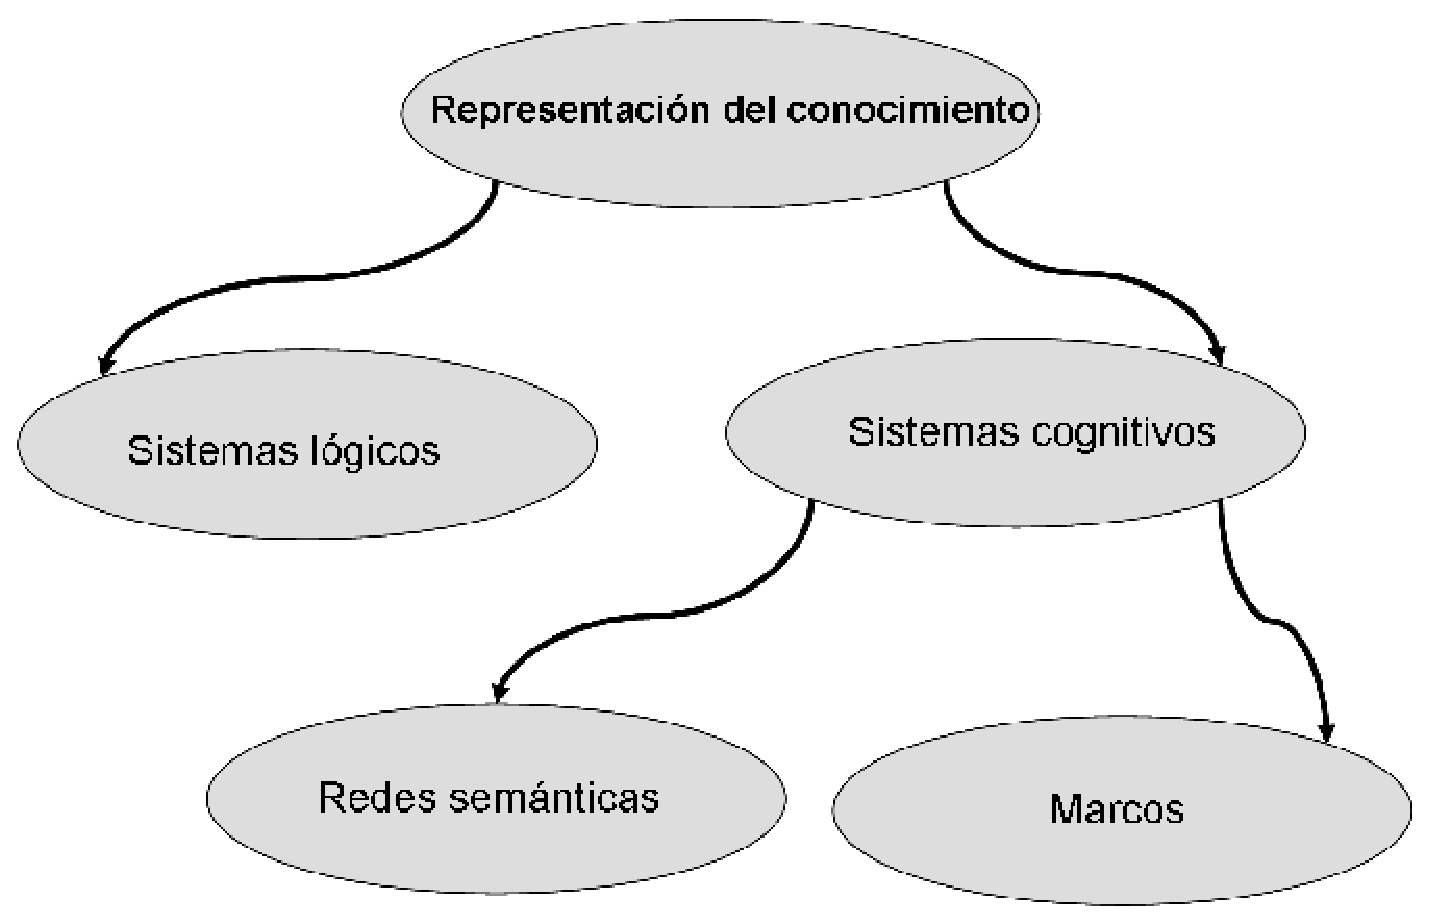
\includegraphics[width=10cm]{images/knowledge}
\caption{Sistemas basados en conocimiento.}
\label{fig:knowledge}
\end{figure}


\subsubsection{Clasificación de ontologías}
Las ontologías se pueden clasificar atendiendo a diferentes a criterios, a
continuación se exponen algunos de ellos.
\begin{description}
 \item [Grado de axiomatización.] Atendiendo a Sowa~\cite{Sowa99knowledge} las ontologías se pueden clasificar en:
\begin{description}
\item[Terminológicas:] define términos y sus relaciones en taxonomías que
involucran tanto relaciones de subtipo y supertipo, como las que relaciona
partes con un todo (\textit{part-whole}), no incluyen axiomas y definiciones
expresadas en lógica o lenguaje formal interpretable por una máquina. Por lo
tanto, existe menos información sobre el dominio modelado pero la simplicidad de
su especificación permite construir ontologías de gran tamaño.
\begin{example}
WordNet base de conocimiento (y datos) léxica.


Fuente: \url{http://wordnet.princeton.edu/}
\end{example}

\item[Formales:] consta de categorías restringidas por axiomas y definiciones
expresadas en alguna lógica formal, con menos conceptos pero preparadas para soportar
un procesamiento automático y servicios de razonamiento.

Una ontología terminológica podrá convertirse en formal a medida que se añadan
axiomas, aunque esta evolución no es ni mucho menos trivial.
\end{description}

\item[Según contexto.] Dependiendo del grado de dependencia del contexto las ontologías pueden ser:
\begin{description}
\item[Dominio:] modelan conceptualizaciones específicas, con restricciones de
estructura y contenido del dominio. Se reaprovecharán sólo en aquellas
aplicaciones que trabajen en ese dominio. Grado de dependencia alto.

\begin{example}
Ontología de medicina \textit{Galen}.


Fuente: \url{http://www.opengalen.org/}.
\end{example}

\item[Generales o de sentido común:] vocabularios o estructuras taxonómicas
genéricas. Alto grado de reaprovechamiento y bajo de dependencia del dominio.

\begin{example}
Cyc y OpenCyc.


Fuente: \url{http://www.cyc.com/}. 
\end{example}

\item[Metaontologías u ontologías genéricas:] ontologías de dominio genérico,
conceptos universales.
\begin{example}
DOLCE: Descriptive Ontology for Linguistic and Cognitive Engineering.


Fuente: \url{http://www.loa-cnr.it/DOLCE.html}. 
\end{example}

\end{description}

\item [Objeto de creación.]

Atendiendo al objetivo de creación de una ontología se establecen diferentes tipos:

\begin{itemize}
  \item Ontologías para la representación de conocimiento, como: \gls{OWL},
  \gls{DAML+OIL}, \gls{RDF}, RDF(S), OKBC, etc.
  \item Ontologías \textit{top level}, definen \textit{frameworks}, conceptos
  universales como las ya comentadas \textit{DOLCE} o \textit{Cyc}. 
  \item Ontologías para la definición de términos lingüisticos como
  \textit{WordNet} o \textit{EuroWordNet}~\cite{EuroWordNet}. 

	\item Ontologías de dominio, modelan conocimiento de cierto dominio: comercio
	electrónico o \textit{e-commerce}, de medicina \textit{Galen} o SNOMED, etc. 
\end{itemize}

\end{description}

Las ontologías como sistemas basados en conocimiento, serán más productivos
cuanto mejor ``informados'' estén, por ello, será interesante modelar utilizando
el mayor de grado de particularidad posible en el dominio, pero teniendo presente, que también es
importante mantener el objetivo de reutilizar conocimiento, podría ser interesante
enclavar los nuevos conceptos de dominio definidos dentro de las categorías de
alto nivel, para así alinear estas definiciones en un marco conceptual genérico.


\subsubsection{Principios de diseño}\label{onto-design}
Las ontologías deben o deberían cumplir una serie de principios:
\begin{description}
\item[Claridad:] proporcionar el significado pretendido a los términos
definidos. Definiciones tan objetivas como sea posible.
\item[Completitud:] las definiciones deberían recoger todas las condiciones
necesarias y suficientes, además de poseer una buena documentación en lenguaje natural.
 \item[Coherencia:] los términos definidos deben ser coherentes, concluyendo
 sólo aquellas inferencias consistentes con el modelo definido.
 \item[Extensibilidad:] anticipando la necesidad de reutilización y facilitando
 la adición de nuevo \linebreak conocimiento.
 \item[Mínimo compromiso ontológico:] minimizar el número de afirmaciones a
 realizar sobre el dominio modelado, permitiendo así que otros agentes las
 puedan refinar.

\item[Diversificación de jerarquías:] haciendo uso de la herencia múltiple, usar
tantos criterios de clasificación como sea posible. Así, añadir un nuevo concepto
es sencillo utilizando los ya existentes y la capacidad de clasificación.

\item[Minimizar la distancia semántica entre hermanos:] conceptos similares
deben agruparse.
 
  \item[Estandarización:] independencia simbólica, utilización de nombrado estándar.
 \item[Granularidad:] coherencia en el grado de particularidad, evitando el uso
 de términos ambig\"{u}os.
\end{description}

Finalmente, existen diversos procesos de desarrollo o metodologías que definen un
procedimiento para la captura de conocimiento de un dominio y la pertinente
construcción de ontologías. Por ejemplo: \textit{Methontology Framework} o \textit{Sensus method}. 


\subsubsection{Operaciones con ontologías}\label{op-ontologias}
En esta sección se describen las
operaciones~\cite{bruijn06-seman-web} que se pueden
realizar con las ontologías de acuerdo a su principio de reaprovechar el
conocimiento ya definido. La reutilización del conocimiento consensuado  es una de las
máximas de la creación de ontologías, para ello se definen tres operaciones
básicas (\textit{mapping} o correspondencia entre ontologías, \textit{merging} o
unión de ontologías y \textit{alignment} o descubrimiento de las
correspondencias de \textit{mapping} ) que
ayudan a la agregación de conocimiento basado en ontologías. La
importancia de estas operaciones se pone de manifiesto en la mediación de datos
entre fuentes heterogéneas, aspirando a resolver los conflictos que se producen
entre sistemas basados en conocimiento, que deben interaccionar entre sí pero que
han sido creados independientemente. El proceso de mediación, adquiere especial
interés para la propuesta de servicios web semánticos, en los cuales esta
operación es básica debido a la integración de ontologías provenientes de
diferentes modelos de negocio.  


\begin{description}
\item[\textit{Mapping} o \textit{mapeo} de ontologías:] especificación declarativa del
solapamiento semántico entre dos ontologías. Las correspondencias entre
entidades de ontologías diferentes son expresadas mediante axiomas en un
determinado lenguaje de \textit{mapeo}. Este proceso consta de tres fases: descubrimiento, representación y ejecución. Existen diferentes enfoques para llevar a cabo esta operación
como MAFRA, RDFT o C-OWL.
\item[\textit{Alignment} o alineamiento de ontologías:] proceso mediante el cual
se descubren las similitudes entre dos ontologías. El resultado es una especificación de los puntos en común, realizada a través del algoritmo 
\textit{Match operator}. Existen diferentes implementaciones como
Anchor-PROMPT, \linebreak GLUE, \textit{Semantic Matching} o QOM.
\item[\textit{Merging} o unión de ontologías:] creación de una ontología nueva
tomando como fuente dos o más ontologías. La nueva ontología unifica y reemplaza
las ontologías fuente. Se establecen dos enfoques para realizar esta
operación: 1) entrada de $n$ ontologías y salida de una sola
ontología, unión y reemplazo de las demás (por ejemplo: algoritmo
PROMPT~\cite{NM00}) y 2) entrada $n$ ontologías que no son reemplazadas, sino que se genera una ontología
\textit{bridge} que importa a las ontologías originales y especifica las correspondencias mediante
axiomas \textit{bridge}, por ejemplo \textit{OntoMerge}.
\end{description}

A la hora de afrontar la implementación de estas operaciones sobre ontologías se pueden generar dos tipos básicos de conflictos que impiden el éxito de la
operación y requieren intervención humana para facilitar la realización
automática de las operaciones: 
\begin{enumerate}
  \item Conflictos entre ``conceptualizaciones'' distintas del mismo dominio. A
  su vez, se distinguen dos categorías: 1) conflicto de ámbito, ocurre cuando dos clases tienen solapamiento en sus extensiones (el
  conjunto $s$ de instancias), y no coincide exactamente y 2) conflicto en la
  cobertura del modelo y su granularidad, ocurre si dos ontologías cubren parte
  de cierto dominio (por ejemplo: empleados de universidad y estudiantes) o bien
si una es más específica que otra (por ejemplo: una ontología define ``persona'' y otra define ``persona joven'').
  \item Conflictos entre las especificaciones de los conceptos. También, se diferencian tres categorías:\linebreak 1) conflicto en el estilo de
  modelado, cada ontología específica los conceptos de una manera determinada
(por ejemplo: tratamiento de las unidades de tiempo) o la descripción de los
conceptos   difiere (por ejemplo: utilización de subclases vs atributos); 2) conflicto
en la  terminología, dos conceptos son equivalentes pero no utilizan el mismo nombre,
  problema de sinónimos, o viceversa, son diferentes y utilizan el mismo nombre,
  homónimos y 3) conflicto de codificación, no se utilizan las mismas
  nomenclaturas, unidades de medida, etc.
\end{enumerate}

Todos estos conflictos, vienen en muchos casos provocados por no ajustarse a los
principios de diseño establecidos en la Sección~\ref{onto-design}. No
obstante, es habitual afrontar los problemas surgidos en la integración de ontologías ya que los
modeladores provienen de distintas partes, con diferente formación y puede que
sigan procedimientos particulares para la realización del modelado de
las ontologías, facilitando las tareas a las aplicaciones que las consuman.


\subsubsection{Aplicación de las ontologías}
Las ontologías se convierten en la pieza fundamental de ciertas áreas así pueden señalarse las 
siguientes:

\begin{description}
\item[Ingeniería del conocimiento:] las ontologías se pueden manifestar durante la ejecución de las siguientes tareas:
\begin{itemize}
  \item Construcción del modelo conceptual, generando los términos del glosario
  y de las relaciones que se establecen entre ellos.
  \item Construcción de la base de conocimiento, utilizando la ontología de
  modelado conceptual se pueden crear bases de conocimiento con la aplicación de
  reglas, restricciones, etc.
\end{itemize}

\item[Procesamiento del lenguaje natural:] mantenimiento de la definición de términos
gramaticales del lenguaje y las relaciones entre ellos.

\item[Integración de sistemas heterogéneos:] gestión de las diferencias
existentes entre diversos sistemas de información con el objetivo de facilitar
la comunicación entre los mismos.
\item[Búsqueda semántica:] utilizando conceptos y no términos para realizar las
búsquedas. 

\item[Web Semántica:] las ontologías son la base de la Web Semántica, por ello
cualquier aplicación que tenga un carácter semántico se apoyará, muy
probablemente, en ontologías.
\end{description}


Las ontologías se abren paso con fuerza sobre todo en el ámbito de las
aplicaciones~\cite{DBLP:conf/nldb/Penalver-MartinezVS11} de la Web Semántica, en particular en el escenario de la
integración de aplicaciones (servicios web semánticos~\cite{DBLP:journals/es/SanchezSMAVG11}) y contextualización del
usuario. En la construcción de una ontología, hay que afrontar el modelado desde el
punto de vista de la lógica (tipo y lenguaje de expresión) siguiendo los
principios de diseño, ver Sección~\ref{onto-design}, y no de la orientación a objetos, muy frecuente en el ámbito de la ingeniería del \textit{software}.  
   
\newpage
\section{\linkeddata}
En los últimos tiempos nos encontramos un entorno de datos fluyendo constantemente, esperando a ser utilizados para generar información
sobre un determinado acontecimiento. De esta manera, podemos ser conscientes de las últimas noticias, productos de una determinada
marca o simplemente sobre información de nuestros contactos en las redes sociales. Esta nueva situación implica que existe un nuevo
mercado para la construcción de aplicaciones y servicios~\cite{Krafzig2004} que exploten estos datos, generando nuevos negocios~\cite{web20} y conectando a las comunidades
científicas, y en general fomentando el progreso de una forma sostenible. Por ejemplo, algunos servicios de búsqueda como Google~\cite{Google} utilizan los
datos publicados en las tiendas de Internet como Amazon~\cite{Amazon}, para extender y procurar resultados de búsqueda más ajustados. En esta línea, prestando 
atención a los resultados de los principales buscadores, las primeras sugerencias corresponden a páginas de Wikipedia~\cite{Wikipedia}, Facebook~\cite{Facebook},
 Linkedin~\cite{Linkedin}, etc.,  por lo que efectivamente queda patente que los servicios de búsqueda~\cite{Pound}, entre otros, están sacando partido de los datos estructurados publicados en distintos sitios web, para así identificar descripciones, organizaciones, personas, perfiles profesionales o productos y 
ofrecer resultados más acordes con la intención de los usuarios.

La evolución hacia esta nueva web, también de denominada Web $3.0$, globalmente enlazada mediante datos supone una transición~\cite{Ankolekar07thetwo}
de la web tradicional orientada a documentos (Web $1.0$) y dirigida hacia las personas principalmente, incluyendo relaciones (Web $2.0$),
a una nueva \wod, en la cual los datos se publican para ser tratados por los humanos como
por los agentes automáticos, proporcionando descripciones más completas a todos los niveles. En este
sentido, Tim Berners-Lee explica convenientemente los principios de esta nueva web realizando una analogía 
de una bolsa de patatas~\cite{TBL-crisps} con una página web, en la cual la parte delantera estaría orientada 
hacia las personas, mientas que la información (meta información) de la parte trasera serían datos
dirigidos hacia otros agentes.

Actualmente la publicación de datos se haya envuelta en distintos dominios en los que previamente
nunca se había pensado compartir datos, pero en los cuales se están generando nuevos servicios y 
oportunidades de negocio a partir de esta iniciativa que busca la compartición de datos. En 
este estado pueden surgir varias preguntas:
\begin{itemize}
 \item ¿Cómo se deben publicar los datos para ser reutilizados?
\item ¿Existen mecanismos para la reutilización automática?
\item ¿Cuál es la forma más ágil para integrar fuentes de datos heterogéneas?
\item ¿Se puede asegurar la calidad de los datos en términos de disponibilidad, autenticidad, evolución, etc.?
\end{itemize}

Estamos, en consecuencia, ante una revolución del uso de datos en la Web, entorno en el cual se pueden realizar
diferentes operaciones sobre los mismos: descubrimiento, consulta, integración y explotación. La Web ofrece
su infraestructura~\cite{webarch}, protocolos y amplio asentamiento para reducir el impacto de esta evolución. No obstante, esta nuevo 
entorno trae consigo nuevos requisitos arquitectónicos, necesidad de entender el comportamiento de las \gls{URI}s~\cite{uri-rfc} y del 
protocolo \gls{HTTP}~\cite{http-rfc} para reutilizar la infraestructura existente y concienciar a la comunidad del empleo de este entorno. 

\subsection{Definición y necesidad de \textit{Linked Data}}\label{def-linkeddata}
Tim Berners-Lee acuñó esta iniciativa en el año 2006~\cite{Berners-Lee-2006} como parte de la Web Semántica~\cite{Berners-Lee2001,WeavingTim,berners-lee06a}. 
En un principio la Web Semántica surgió con el objetivo de integrar grandes bases de datos a través de modelos de conocimiento compartidos u ontologías, de esta manera
cualquiera podría reutilizar el conocimiento ya consensuado y en consecuencia los datos asociados a esta información. Si bien
la Web Semántica tuvo un gran éxito desde un punto de vista teórico, en la práctica escasas aplicaciones reales llegaron a tener
un notable impacto en el gran público~\cite{sw-use-cases}. Es por ello, que tomando la visión de la Web Semántica en su parte de modelos y formatos de datos
estandarizados formalizados a través de conocimiento compartido, fue tomada para definir lo que actualmente conocemos como \linkeddata~\cite{linked-data}.
En realidad se trata de un enfoque práctico de la Web Semántica, en el cual
se hace uso de los fundamentos de la semántica y de la web para proveer mecanismos para la publicación~\cite{bizer07how,Berr08} y 
consumo de datos masivos sin tener grandes barreras de entrada y claramente orientado al desarrollo de aplicaciones. 
Análogamente en el arranque de la web orientada a documentos se realizó un esfuerzo para la identificación sobre cómo publicar documentos, por ejemplo utilizando HTML, pero no se hizo hincapié en
modelar la información que se publicaba en los mismos, esto ocasionó que la Web que hoy conocemos despegara exponencialmente. En el caso
de la \wod se realiza un enfoque similar, es decir, se establece cómo publicar datos, sin embargo no realiza especial énfasis
 en que estos datos estén formalizados estrictamente sobre un modelo conocimiento. De esta manera se facilita y favorece el crecimiento y la aparición de nuevas fuentes
de datos en la Web. No obstante, esta segunda parte de modelado y estructuración de datos deviene fundamental para ciertas tareas
automáticas.

El objetivo por lo tanto de la \wod no se centra tan sólo en publicar datos sino en hacer los datos accesibles, tanto a las personas
como a las máquinas, como son actualmente los documentos disponibles en la Web. La diferencia sustancial reside en que actualmente
la web está orientada al uso por personas y las máquinas necesitan de procesos de un cierto grado de complejidad para acceder a esta información.
Por lo tanto, con esta nueva iniciativa se facilitan los enlaces entre los datos para que puedan ser explorados eficientemente 
por cualquier agente y realizar operaciones de enriquecimiento y enlazado de forma sencilla.

La \wod se construye sobre enlaces como la web tradicional en la que los documentos son enlazados entre sí. La diferencia
reside en que los datos utilizan enlaces en \gls{RDF} para describir recursos de distintos tipos identificados de forma unívoca
mediante un \gls{URI} y siguiendo unos principios que, aunque analizados en detalle en la Sección~\ref{principos-linked-data}, se presenta a continuación una breve descripción de los mismos:
\begin{itemize}
 \item \textit{Use URIs as names for things}. Utilizar URIs como nombres para identificar y acceder a los recursos.
 \item \textit{When someone looks up a URI, provide useful information, using the standards (RDF*, \gls{SPARQL}~\cite{Sparql})}. El acceso 
a los recursos a través de URIs debe estar basado en estándares como RDF o SPARQL suministrando igualmente información
sobre el acceso.
\item \textit{Include links to other URIs. so that they can discover more things}. Enlazar datos no sólo implica la publicación
masiva de datos sino que se deben establecer enlaces entre ellos con el objetivo de proveer un entorno navegable~\cite{Berners-lee06tabulator:exploring,Pietriga06fresnel}.
\item \textit{Use \gls{HTTP URI}s so that people can look up those names}. Utilizar URIs HTTP para reaprovechar la actual infraestructura
de la web y que el público potencial pueda acceder a los datos de la misma forma que hoy lo hace con los documentos.
\end{itemize}

En este contexto formalizado con reglas muy explícitas, queda patente 
que uno de los factores clave de esta iniciativa está en el poder de reutilizar información bien 
estructurada desde la propia fuente de datos, facilitando así la creación de aplicaciones fiables en el 
sentido del tratamiento de datos y evitando el uso de otras técnicas basadas en estadística y procesamiento
de lenguaje natural, que se siguen aplicando ya que no siempre se cumple con todos los requisitos que la iniciativa de \linkeddata establece.

En resumen, el objetivo de la iniciativa de \linkeddata es enlazar datos de fuentes heterogéneas entre sí, 
con el objetivo de enriquecer la información y ofrecer a todos los agentes tanto personas como máquinas
un espacio homogéneo basado en estándares para la realización de las operaciones citadas anteriormente, descubrimiento, acceso y explotación. 
Para ello se hace uso de la tecnología semántica \gls{RDF} que provee una forma flexible y escalable para la realización de descripciones de las entidades 
del mundo: personas, organizaciones, localizaciones, etc. Las sentencias en RDF permiten
establecer de una forma sencilla enlaces entre ellas creando conexiones desde un entorno local
hacia un entorno global. También cabe destacar que el uso de RDF difiere de los actuales
documentos presentes en la web en dos puntos importantes:

\begin{itemize}
 \item El enlace se produce a nivel de entidades, no de documentos.
 \item Cada enlace tiene un tipo definido.
\end{itemize}

\linkeddata permite así establecer conexiones entre diferentes fuentes de datos y crear un espacio 
de datos global, esto es posible gracias al uso de estándares y de un modelo de datos común que facilita
la creación de aplicaciones de carácter general capaces de operar en este nuevo espacio de datos.

El gran valor de \linkeddata se centra por tanto en brindar una oportunidad para utilizar los datos
y explotar su valor mediante sistemas basados en conocimiento, con capacidad de procesar una cantidad
masiva de datos obteniendo así soluciones más fiables y aproximadas a las necesidades y expectativas
de los agentes. En síntesis, ver Tabla~\ref{tabla:linked-data}, se pueden establecer una serie de características y criterios a satisfacer.
\begin{longtable}[c]{|l|p{7cm}|p{8cm}|} 
\hline
  \textbf{ID} & \textbf{Directriz} &  \textbf{Descripción} \\\hline
\endhead
   \multicolumn{3}{|c|}{\textbf{Principios Linked Data}}  \\ \hline
   1.1&\textit{Use URIs as names for things} & \\ \hline
   1.2&\textit{When someone looks up a URI, provide useful information, using the standards (RDF*, SPARQL)} & \\ \hline  
   1.3&\textit{Include links to other URIs} & \\ \hline    
   1.4&\textit{Use HTTP URIs} & \\ \hline    
  \multicolumn{3}{|c|}{\textbf{Modelo $\star$}}  \\ \hline
     2.1&$\star$	& \textit{Available on the web (whatever format) but with an open licence, to be \opendata} \\ \hline 

2.2&$\star \star$	 &  \textit{Available as machine-readable structured data (e.g. excel instead of image scan of a table)} \\ \hline 

2.3&$\star \star \star$	&  \textit{ as (2) plus non-proprietary format (e.g. \gls{CSV} instead of exce}l) \\ \hline 

2.4&$\star \star \star \star$	&  \textit{All the above plus, Use open standards from \gls{W3C} (RDF and SPARQL) to identify things, so that people can point at your stuff} \\ \hline 
 
2.5&$\star \star \star \star \star$	 & \textit{All the above, plus: Link your data to other people’s data to provide context}                                     \\ \hline 
  \hline
  \caption{Características a tener en cuenta sobre \linkeddata.}
  \label{tabla:linked-data}
\end{longtable}

\subsection{\opendata}\label{opendata-sect}
Este término se enclava dentro de las definiciones de conocimiento abierto realizadas por
la organización \textit{Open Knowledge Foundation}~\cite{okfn} (\gls{OKFN}), en el cual también se incluyen:
\begin{itemize}
 \item Contenidos como libros, películas, música y cualquier otro material con autoría definida.
\item Datos, en general, pertenecientes a distintos contextos: científicos, históricos o geográficos.
\item Información proveniente de las Administraciones Públicas.
\end{itemize}

Siguiendo la definición realizada por esta institución, cuando una obra o datos satisfagan las siguientes
condiciones serán consideradas como abiertas:

\begin{description}
 \item [Acceso.] La obra debe estar disponible íntegramente y sólo a un coste de 
  reproducción razonable, preferiblemente para su descarga de modo gratuito en Internet. 
  La obra también debe estar disponible en una forma conveniente para ejecutar modificaciones sobre ella.
 \item [Redistribución.] La licencia no debe contener restricciones sobre la posibilidad de venta o 
  distribución de la obra en sí misma o formando parte de un paquete constituido por obras de fuentes diversas. 
  La licencia no debe exigir un pago u otro tipo de cuota para esta venta o distribución.
 \item [Reutilización.] La licencia debe permitir hacer modificaciones y obras derivadas facultando que éstas sean distribuidas en las mismas condiciones que la obra original. La licencia puede imponer algún tipo de requisito relativo al 
  reconocimiento y a la integridad: veáse el principio 5 (Reconocimiento) y el principio 6 (Integridad) reseñados más adelante.
 \item [Ausencia de restricciones tecnológicas.] Se debe proporcionar la obra de modo que no presente ningún obstáculo tecnológico para ejecutar los actos mencionados anteriormente. Esto se puede conseguir ofreciendo la obra en un formato de datos abierto, por ejemplo un formato cuya especificación esté disponible públicamente y de manera gratuita y que para su uso no se imponga ninguna restricción de tipo monetario o análogas.
 \item [Reconocimiento.] La licencia puede exigir como condición para la redistribución y la reutilización el reconocimiento de los contribuyentes y creadores de la obra. Si se impone esta condición, no debe ser de manera onerosa. Por ejemplo si se exige un reconocimiento, la obra debería ir acompañada de una lista de aquellos que hay reconocer.
 \item [Sin discriminación de personas o grupos.] La licencia no debe discriminar a ninguna persona o grupo de personas.
 \item [Sin discriminación de ámbitos de trabajo.] La licencia no debe contener restricciones sobre el uso en un ámbito de trabajo específico. Por ejemplo, no se puede limitar el uso de la obra en un negocio, o que ésta sea utilizada para investigación militar.
 \item [Distribución de la licencia.] Los derechos adjuntos a la obra deben aplicarse también a todo áquel a quien le sea redistribuida, sin necesidad de que éste disponga una licencia adicional.
 \item [La licencia no debe ser específica de un paquete.] Los derechos adjuntos a la obra no deben depender de que la obra forme parte de un paquete particular. Si la obra se extrae de ese paquete y se utiliza o se distribuye en las condiciones de la licencia de la obra, todos aquellos a quien les sea redistribuida deberán tener los mismos derechos que los concedidos conjuntamente con el paquete original.
 \item [La licencia no debe restringir la distribución de otras obras.] La licencia no debe imponer restricciones en otras obras distribuidas conjuntamente con la obra objeto de la licencia. Por ejemplo, la licencia no debe imponer que todas las otras obras que se distribuyan por el mismo medio sean abiertas.
\end{description}

La corriente de datos abiertos~\cite{odfn} ha sido especialmente acogida en el ámbito de las Administraciones
Públicas, ver Figura~\ref{fig:od-spain}, adaptando las directrices aquí fijadas para desplegar el movimiento
de \ogd. 

\begin{figure}[!htb]
\centering
	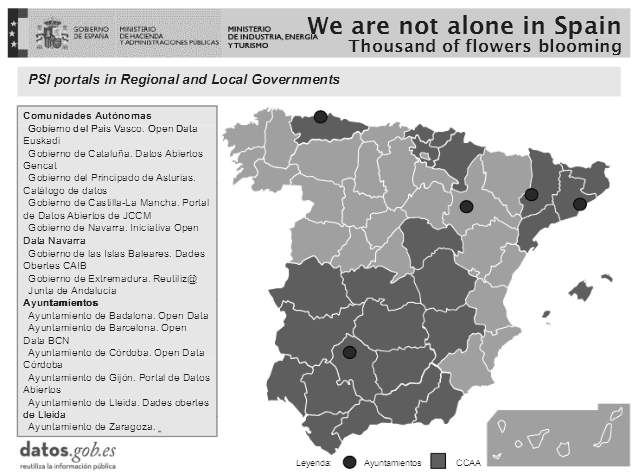
\includegraphics[width=14cm]{images/phd/open-data-spain}
\caption{Estado de \opendata en España}
\label{fig:od-spain}
\end{figure}

Las instituciones públicas han establecido distintos canales de comunicación~\cite{improvingW3c}
con los ciudadanos, intentando siempre mejorar la interacción en los distintos
procesos administrativos. Por ello y para estar presentes en las principales iniciativas
de comunicación han procurado atender a los avances tecnológicos. Desde
principios de la década de los años 90 han tenido presencia en la web proveyendo
distintos servicios para que el ciudadano pueda agilizar sus trámites
y así obtener una administración más eficiente, tanto en tiempo como en uso
de recursos. Esta situación ha derivado a lo que se denomina como ``administración
electrónica'' o \egov, en la cual la información de los servicios
y datos que obran en poder de la Administración resultan de fácil acceso a los
 ciudadanos a través de los principales canales de comunicación, 
como la web, dispositivos móviles, etc., creando de esta forma
una administración con una ventanilla única, fijando como objetivo principal
 la transparencia y la objetividad, materializadas a través de distintas
políticas, concretamente en el caso europeo se dispone de un Plan de Acción~\cite{policy-eu} específico para el período 2011-2015.

No obstante, aunque las intenciones están acertadamente fijadas existen muchos
desafíos que han estado y están impidiendo el despegue definitivo de la administración
electrónica, desde la tecnología hasta el necesario cambio tanto para los
integrantes de la propia administración como para los ciudadanos. Proveer
servicios y datos a través de la red se ha convertido en un desafío en el cual
las distintas administraciones se encuentran inmersas, esta situación
implica ejecutar una gran inversión para dar cabida a todas las necesidades desde un punto
de vista tanto en materia de infraestructura como de concienciación social. De esta forma,
un gobierno basado en administración electrónica debe ser capaz de fijar los requisitos
de los servicios y datos a liberar, asegurar la autenticidad y definir la legislación
pertinente que establezca un marco jurídico seguro para que los ciudadanos pueden utilizar
toda la información disponible para consultar o construir nuevos servicios de valor
añadido sobre ellos.

Entre las actividades que se presentan como claves para el desarrollo de la administración
electrónica se pueden referir los siguientes:
\begin{itemize}
 \item Uso y aplicación de estándares.
 \item Transparencia y participación.
 \item Concienciación de los avances en la gestión e integración de datos.
 \item Relaciones y colaboraciones.
\end{itemize}

En este contexto se determinan por una parte los objetivos de la administración
respecto a disponer un entorno flexible y dinámico para sus ciudadanos, y por otra parte 
se encuentra el comportamiento de las propias personas y organizaciones. Actualmente
se advierte un entorno definido por las siguientes características: 
global, conectado, cambiante y accesible en su mayor parte.

El término de \ogd ha sido designado en la administración de Estados Unidos para indicar
aquellos datos o registros de información que obran en poder de la Administración Pública y que
han sido recabados con distintos objetivos en los distintos procesos administrativos. Como ejemplos
de reutilización en el sector público encontramos los siguientes dominios: salud, cartografía, datos
meteorológicos, educación, datos bibliográficos, contratación pública, legislación, etc. Como 
se ha comentado con carácter previo, las organizaciones públicas producen, almacenan y distribuyen distintos tipos
de información: legal, financiera, geográfica, etc., en su actividad diaria. Esta información
proveniente del sector público (\gls{PSI}) está enclavada dentro de un marco jurídico, por ejemplo en Europa la Directiva 2003/98/EC~\cite{d2003,d2003-update},
 que puede variar de un país a otro, en España la Ley 37/2007~\cite{l37-2007} y su Real Decreto 1495/2011~\cite{r-1495} 
de desarrollo, Reino Unido~\cite{uk2012}, Francia~\cite{fr2012} o la iniciativa de la Casa Blanca en Estados Unidos~\cite{usa}. 
Habitualmente se utilizaban distintas técnicas y formatos
para la distribución de la información del sector público por diferentes canales desde el papel y correo postal, hasta
formatos electrónicos y las propias páginas web. La evolución en los últimos
años ha sido de gran calado de modo que ha hecho necesario dictar una legislación común que 
debe ser transpuesta en los diferentes países, como ocurre en el caso de Europa.

La transición hacia este nuevo enfoque administrativo todavía se encuentra
en una etapa temprana debido a las dificultades que supone toda una nueva forma de
actuar. En general, se suele hablar de \gd y \pusi para referirse al mismo concepto. Se han realizado diferentes definiciones como las
presentes en la iniciativa \ogd, pero no sólo se trata de exponer de forma pública 
las grandes bases de datos gubernamentales, sino que éstos deberían cumplir 
unos principios~\cite{8-principles} que a continuación se listan:

\begin{enumerate}
 \item Data Must Be \textit{Complete}. \textit{All public data are made available. Data are electronically stored information or recordings, including but not limited to documents, databases, transcripts, and audio/visual recordings. Public data are data that are not subject to valid privacy, security or privilege limitations, as governed by other statutes.}
 \item Data Must Be \textit{Primary}. \textit{Data are published as collected at the source, with the finest possible level of granularity, not in aggregate or modified forms.}
 \item Data Must Be \textit{Timely}. \textit{Data are made available as quickly as necessary to preserve the value of the data.}
 \item Data Must Be \textit{Accessible}. \textit{Data are available to the widest range of users for the widest range of purposes.}
 \item Data Must Be \textit{Machine processable}. \textit{Data are reasonably structured to allow automated processing of it.}
 \item Access Must Be \textit{Non-Discriminatory}. \textit{Data are available to anyone, with no requirement of registration.}
 \item Data Formats Must Be \textit{Non-Proprietary}. \textit{Data are available in a format over which no entity has exclusive control.}
 \item Data Must Be \textit{License-free}. \textit{Data are not subject to any copyright, patent, trademark or trade secret regulation. Reasonable privacy, security and privilege restrictions may be allowed as governed by other statutes.}
\end{enumerate}

Con todo ello, se provee un entorno en el cual ``público'' designa a las condiciones que deben cumplir los datos
para considerarse ``abiertos'', no se entra a valorar los datos que se deben liberar ni tampoco cuestiones
legales. En cuanto a los ``datos'', se toma este término para designar a los registro electrónicos, es importante
destacar que los documentos físicos no se consideran como tal, que obran en poder de la administración y finalmente,
con ``revisable'' se denomina a aquellos datos para los cuales existe una persona de contacto que actúa como
enlace para aquellos que quieran usar los datos, para gestionar el uso de los mismos y para los cuales
existe un organismo administrativo o judicial que posee la potestad para aplicar los principios antes
citados adecuadamente.

Por otra parte, existen cuestiones~\cite{publishing-ogd} que deben tener respuesta en el contexto de \ogd desde un punto
de vista estratégico hasta funcional como qué tipo de interfaz de acceso (\gls{API}) se debe proveer para el acceso a los datos, por ejemplo, 
en cuanto a los datos a liberar, la iniciativa de datos abiertos no especifica qué datos deberían liberarse. Corresponde
a la estrategia del organismo en cuestión establecer las prioridades, coste y beneficios de la liberación de un determinado conjunto
de datos. En determinados casos como el del Gobierno de Reino Unido~\cite{uk-survey} o el Ayuntamiento de Zaragoza~\cite{zar-survey} se utilizan encuestas
a los propios usuarios para especificar o establecer un orden en los datos a liberar. El objetivo final será
disponer de una política y guías de apertura de datos que sean capaces de dar soporte a los siguientes puntos:

\begin{description}
 \item [Inclusión.] El uso de estándares facilita la accesibilidad y la usabilidad de los datos. De esta forma,
se facilita la participación de terceros y el desarrollo de aplicaciones de distinto carácter que beneficiarán
transversalmente a toda la sociedad con nuevos servicios.
\item [Transparencia.] En los últimos años y debido a los múltiples casos de corrupción a nivel político, deficiente gestión
de fondos públicos y en general, cierta falta de claridad por parte de las instituciones ha hecho que esta corriente
se sitúe como un eje el impulso de la transparencia en el conjunto de las administraciones públicas.
\item [Responsabilidad.] La eficiencia en el uso de recursos debe ser uno de los objetivos de la administración pública, por ello
conseguir información sobre cómo funciona la administración puede permitir mejorar su funcionamiento interno.
\end{description}

Una vez que se dispone de datos abiertos cabe definir cómo se pueden obtener mejoras en ciertos procesos de uso. Entre 
ellos se puede destacar:

\begin{description}
\item [Reutilizar.] La información abierta permite plantear nuevos modelos de interacción, tanto para otras administraciones públicas
como para organizaciones o comunidades que se beneficien de estos datos para el despliegue de nuevos servicios~\cite{web20}. Actualmente
se realizan actividades para el impulso de la reutilización de datos, como los concursos en los que se liberan datos a los que interesados
presentan aplicaciones haciendo uso de ellos.
 \item [Generar múltiples vistas de los datos~\cite{DBLP:journals/semweb/DadzieR11}.] Cuando se dispone de los datos de una forma más o menos estandarizada y con facilidad
de acceso se pueden generar múltiples vistas, dependiendo de las necesidades del usuario y adaptándolos al contexto. Por ejemplo,
generación de informes en PDF, visualización en mapas de la información geográfica, etc. Partiendo de los mismos datos y en algunos
casos y tras la ejecución de un proceso de enriquecimiento se puede mejorar la información que provee. El coste de realización de 
estos procesos es alto si está centralizado en la administración, pero se puede diversificar y abaratar delegando en 
terceras partes.
 \item [Mejorar los actuales sistemas de búsqueda~\cite{hoga-etal-2011-swse-JWS}.] Un sistema de búsqueda dispondrá de mayor precisión cuanto más ``informado'' esté, por lo tanto,
si se pueden reutilizar los datos ya disponibles para mejorar los resultados de las consultas de los usuarios, se facilitará el acceso a la
información.
  \item [Integrar fuentes de datos~\cite{Andreas_Schultz_Isele_Bizer_Becker_2011,Harth:2011:SIP:1963192.1963318}.] Habitualmente cada organismo goza de cierta independencia para gestionar sus propios datos. La realidad
es que en muchos casos diferentes organismos de la misma entidad tienen la necesidad de cruzar datos para obtener diferente información
agregada. Si se utilizan datos abiertos se favorece la integración y la reutilización de datos disminuyendo los costes de la obtención
y gestión de los mismos al no estar multiplicada.
\end{description}

Una vez que se han definido algunos de los beneficios del uso de datos abiertos en el ámbito de las
administraciones públicas, cabe ahora especificar cómo han de ser publicados para que
puedan ser consumidos por terceros de forma ágil. Para ello se han establecido una serie
de directrices o métodos:
\begin{itemize}
 \item Usar anotaciones basadas en microformatos o \gls{RDFa}~\cite{rdfa-primer} en \gls{XHTML} o \gls{HTML}5~\cite{HTML5}.
 \item Facilitar la accesibilidad siguiendo las directrices \gls{WCAG}~\cite{wcag2}.
 \item Desplegar APIs específicas para el consumo de datos.
 \item Sindicar de contenidos mediante \gls{RSS}~\cite{rss} o \gls{ATOM}~\cite{atom-rfc}.
 \item Proveer interfaces \gls{REST}~\cite{Fielding2000} o \gls{SOAP}~\cite{SOAP11} de servicios de acceso a datos.
 \item Aplicar tecnologías semánticas mediante \gls{RDF}.
\end{itemize}

Finalmente se ha de definir la misión y estrategia de apertura de datos, así la confianza (\trust), procedencia~\cite{Carroll05namedgraphs,prov-group} (\provenance) y calidad de los mismos, la
evolución en tiempo, las limitaciones tecnológicas y la capacidad para seguir creciendo. De acuerdo a lo expuesto en esta sección se pueden
establecer una serie de factores a evaluar sobre la publicación de datos abiertos de acuerdo a distintos criterios y que 
servirán para evaluar si se cumplen las guías definidas. 

\subsection{\lod}
La convergencia entre las iniciativas de \linkeddata y \opendata ha conllevado la creación
de un nuevo término para designar a aquellos datos que cumplen las guías de ambas iniciativas y que 
se denomina \lod. Bajo esta definición se agrupan todos los datos que han sido
liberados aplicando los principios de \linkeddata y que además cumplen significativamente
las directrices de \opendata. Habitualmente este término se aplica en el contexto de las Administraciones
Públicas, en las que el esfuerzo por la apertura de datos ha sido intenso y en el que han logrado grandes avances. 

El alto valor de los datos enlazados abiertos permite disfrutar a terceros de la posibilidad real 
de creación de servicios de alto valor añadido. No obstante, surge la duda de si el proceso de enlazado de datos
y de explotación, corresponde a la propia Administración o si cabe delegar el mismo. En este sentido, existen
una serie de cuestiones que se han de plantear:
\begin{description}
 \item [¿Debe la Administración explotar los datos y construir aplicaciones para su consumo?] En un primer momento, las Administraciones
Públicas cubrían toda la cadena valor de uso de los datos, desde su apertura hasta su explotación. En estos momentos, se está produciendo
un cambio de dirección en cuestiones de sostenibilidad que implica que la creación de servicios y aplicaciones se delega en terceros. Si bien
como punto de partida es conveniente que la Administración demuestre el valor del uso de los datos, una vez que se ha producido
la sensibilización necesaria resulta evidente que deben ser terceras partes quienes reutilicen los datos.
\item [¿Qué nivel de \linkeddata debe proveer la Administración?] El caso ideal sería que los datos liberados se encontrarán
en el estatus de 5 $\star$ pero la realidad es que tanto por parte de la comunidad de desarrolladores, habituados
a tecnologías como \gls{RSS} o APIs \gls{REST}, como por el propio coste
que genera llegar a este nivel, en muchos casos no es realmente útil realizar este esfuerzo, con la simple apertura de datos
y un modelo de acceso convenientemente homogéneo es suficiente.
\item [¿Sobre la calidad de los datos?] Como se ha comentado es fundamental para motivar la creación de aplicaciones
la confianza en los datos que se están utilizando. En este sentido poder verificar su procedencia, evolución en el tiempo, autenticidad
y en general, su nivel de confianza y calidad es vital para el triunfo de esta corriente en aplicaciones de alto valor añadido. El esfuerzo
de la Administración debe centrarse por consiguiente en este punto, asegurando a la comunidad la confianza en los datos
que van a usar.
\item [¿Qué estructura se debe seguir en los organismos públicos para liberar los datos?] Existen principalmente dos enfoques
para abordar la apertura de datos masiva: \textit{top-down} y \textit{bottom-up}. El enfoque \textit{top-down} se está
utilizando en el Gobierno de Reino Unido y consiste básicamente en fijar las directrices, modelos, etc., que se han de seguir para liberar
datos desde un organismo central que propaga esta metodología a todos los sectores y organismos públicos que deseen abrir sus datos. Por el contrario,
el enfoque \textit{bottom-up} tiene su paradigma en la Administración española en el cual han surgido numerosos conjuntos de datos aplicando
sus propias directrices. Determinar cuál es el mejor modelo depende del nivel de precisión que se establezca en cuanto a la publicación de datos, en contraposición
con el coste del mismo y el tiempo empleado. El enfoque \textit{top-down} si bien es más homogéneo, requiere un enérgico esfuerzo común inicial tanto en tiempo
como en coste, pero en el largo plazo es más sostenible puesto que todos los organismos reaprovechan la experiencia. En cambio, el enfoque \textit{bottom-up} permite
un despliegue inicial más rápido multiplicando el esfuerzo y los costes en cada organismo candidato a la apertura de datos, pero 
con la posibilidad de que uno de los modelos particulares se convierta en referente.
\item [¿Cómo se debe prevenir la privacidad de los datos?] Si bien por la propia definición de datos enlazados abiertos no se debiera tener
en cuenta esta cuestión, si que surge la necesidad en contextos determinados ofrecer mecanismos de control para prevenir el uso inadecuado
de datos, por ejemplo los denominados ``secretos estadísticos'' y así evitar infringir otras leyes como las referidas a datos personales.
\item [¿Puede la Administración establecer un modelo de negocio, ver Figura~\ref{fig:data-business-model}, sobre los datos?] Este punto genera cierta controversia, ya que el coste de posesión 
de los datos recae sobre los ciudadanos, actualmente cualquier servicio público o proceso administrativo tiene unos costes que se financian
a través de determinadas tasas. En el caso de la apertura de datos se considera que no debe suponer un coste adicional para los administrados
pero la realidad es que el coste implícito está presente, es más, algunos organismo utilizan este mecanismo como medio de auto-financiación. Desde un punto
de vista de los agentes implicados, los terceros que utilicen estos datos no estarán dispuestos a pagar un sobrecoste por su uso, la propia Administración
no estaría incentivada a la aplicación de tasas sobre estos datos presumiendo que el retorno provisto de terceros sea capaz de financiar la apertura de los datos. Reiterando que 
por definición los datos deberían ser libres también es necesario la creación de un entorno sostenible y probablemente el enfoque óptimo en el 
estadio inicial sea de conformidad a un modelo libre.
\item [Otras cuestiones.] Relacionadas con los datos a liberar, realimentación de los mismos (\textit{crowdsourcing}) para corregir errores, reconciliación, etc. siguen todavía abiertas y obtendrán respuesta paulatinamente, en función la propia demanda.
\end{description}

\begin{figure}[!htb]
\centering
	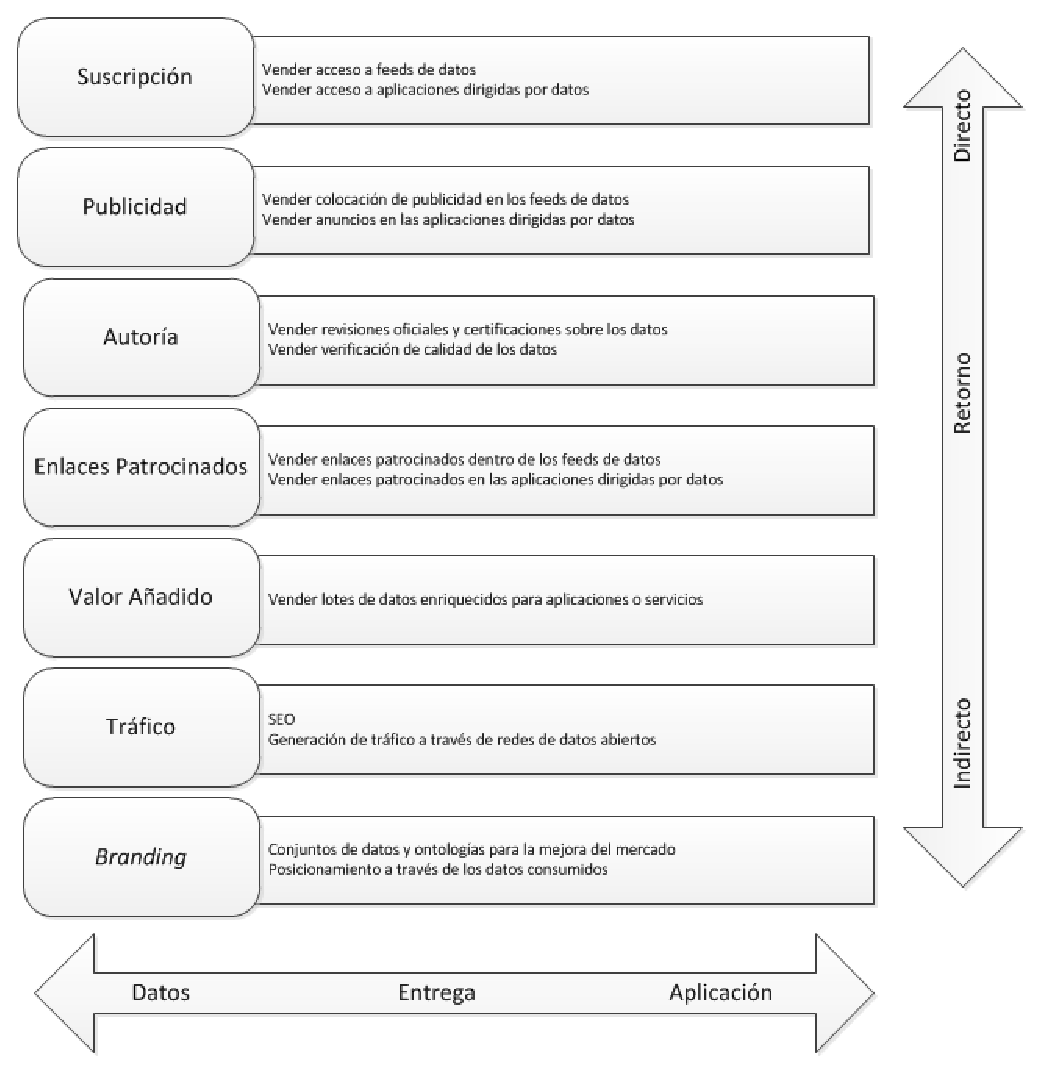
\includegraphics[width=12cm]{images/phd/data-business-models}
\caption{Modelos de negocio para datos (extraída de \textit{Chief Marketing Technologist}).}
\label{fig:data-business-model}
\end{figure}


En definitiva, la conjunción de los principios de \linkeddata y \opendata ha conllevado una corriente de actuación
en las Administraciones Públicas con amplios beneficios tanto para los ciudadanos como para las empresas. La experiencia inicial es altamente
enriquecedora para las partes implicadas y su tendencia es seguir creciendo. No obstante, también se presentan varias cuestiones
abiertas que se habrán de ir resolviendo a la vez que la tecnología y la experiencia se incrementan.
\subsection{Principios de \linkeddata}\label{principos-linked-data}
En las secciones anteriores se han repasado las líneas que marcan la definición de \linkeddata, se pueden resumir
en una corriente que aúna la tecnología semántica más madura con la apertura de datos, en un infraestructura perfectamente
establecida como es la Web.

Los principios de \linkeddata~\cite{Berners-Lee-2006} se reducen a los siguientes cuatro puntos:

\begin{itemize}
 \item \textit{Use \gls{URI}s as names for things}. La utilización de URIs como nombres para identificar y acceder a los recursos. Este principio busca el uso de URIs como camino para referenciar de forma única a todos
los recursos disponibles, no sólo documentos, así: contenidos digitales, vídeos, sensores~\cite{ontology-search,Jeung:2010:EMM:1850003.1850235}, 
  organizaciones~\cite{open-corporates}, personas~\cite{facebook-ld}, etc., con el objetivo de ampliar el contexto de un espacio virtual a uno real.
 \item \textit{When someone looks up a URI, provide useful information, using the standards (RDF*, SPARQL~\cite{Sparql})}. El acceso 
a los recursos a través de URIs debe estar basado en estándares como \gls{RDF} o \gls{SPARQL} proveyendo igualmente información
sobre cómo acceder.
\item \textit{Include links to other URIs. so that they can discover more things}. El enlazado de datos no sólo implica la publicación
masiva de los mismos, sino que se deben establecer enlaces entre ellos con el objetivo de proveer un entorno 
navegable~\cite{Berners-lee06tabulator:exploring,Pietriga06fresnel} y de consulta~\cite{Hartig09executingsparql}.
\item \textit{Use \gls{HTTP URI}s so that people can look up those names}. La utilización de URIs HTTP para reaprovechar la actual infraestructura
de la web y que el público potencial pueda acceder a los datos de la misma forma que se realiza actualmente con los documentos.
\end{itemize}

En general estos principios buscan una manera estándar de identificar, modelar, acceder y consumir recursos para que la creación
de aplicaciones y servicio sea lo más sencilla y ágil posible.

Por lo tanto, para atender a estos principios se deben facilitar una serie de mecanismos que permitan:
\begin{itemize}
 \item Nombrar a todas las cosas, recursos, etc., mediante URIs.
 \item Referenciar y acceder a los contenidos mediante URIs. Uso de \textit{hash}, \textit{slash} URIs o código $303$ de \gls{HTTP}. 
 \item Proveer información útil sobre los recursos de forma estándar mediante RDF. Uso de literales o de enlaces a otras
descripciones RDF. Negociación de contenido.
 \item Incluir enlaces a otros datos. Podemos establecer tres tipos de enlaces principales: relación, identidad y 
vocabulario. Cada uno permite establecer relaciones, alinear unos recursos con otros y definir las descripciones
respectivamente.
\end{itemize}

Los beneficios de la utilización de estos mecanismos que sustentan a los $4$ principios citados proporcionan las siguientes ventajas:
\begin{itemize}
 \item Escala global. El uso de \gls{RDF} permite unificar la información de los recursos, modelo, formato y acceso a los datos.
 \item Enlace entre recursos. RDF da soporte a la reutilización intrínseca de recursos ya definidos dando cabida
a la unión de datos de diferentes fuentes.
  \item Expresividad. La información en RDF se puede representar combinando distintos vocabularios.
 \item Estructuración. Utilizando un modelo definido en RDF(S) u \gls{OWL} se da soporte al modelo de los datos
mediante mecanismos estándar, compartidos y reutilizables.
\end{itemize}

Además de estas ventajas, existen ciertas características que deberían evitarse, tales como los mecanismos
de reificación de RDF, las colecciones o el uso de nodos en blanco con el objetivo de facilitar la consulta
mediante el lenguaje SPARQL. En cuanto a los formatos en los que se pueden presentar los datos enlazados en RDF se encuentra:
\gls{RDFa}~\cite{rdfa-primer}, \gls{RDF/XML}~\cite{rdf-syntax}, \gls{Turtle}~\cite{turtle-syntax}, \gls{N3}~\cite{n3-syntax} ,\gls{RDF}/\gls{JSON}~\cite{rdf-binario} o RDF binario~\cite{rdf-json}.


En definitiva, se trata de proveer un entorno estándar y global de datos en el cual se utilice un modelo
de datos estandarizado y único (RDF), con capacidad para enlazar a otros datos y que todos ellos se auto-describan
en el sentido de facilitar a sus descripciones beneficiando el descubrimiento, acceso e integración de datos.

\subsection{Construyendo una nueva \wod}
Este nuevo entorno de publicación de datos ha implicado que numerosas personas y organizaciones
se hayan inclinado por la aplicación de los principios de los datos enlazados en la apertura de sus datos. Como resultado
se puede establecer que el despegue de la \wod es ya un hecho, creando un grafo global de billones
de tripletas RDF de diferentes tipos y fuentes enlazadas~\cite{HoganUHCPD:2012:237} entre sí. En general, esta eclosión se debe
a varias razones: genericidad, estandarización, dominio público, capacidad de representación de la información, expresividad,
reutilización de tecnología estable, etc. Como origen de este enfoque se puede situar la iniciativa
del \lod~\cite{lod-group} (\gls{LOD}) del W3C en el año 2007, en el cual se sentaron las bases de la actual \wod, dando comienzo el desarrollo tecnológico así como la transformación de los primeros conjuntos de datos. Entre ellos
podemos destacar el esfuerzo de la DBPedia~\cite{dbpedia2009} o herramientas como \gls{Pubby}, D2RServer, etc. La evolución
de la \wod queda recogida en el diagrama de la nube de \datasets (\textit{LOD Cloud}~\cite{linked-data-cloud}) que en su última
versión recoge hasta 320 \datasets, ver Figura~\ref{fig:lod-cloud}, y continua en aumento si se consulta \textit{The Data Hub}~\cite{the-data-hub}. A modo informativo a fecha de septiembre
de 2010 en el diagrama anteriormente citado estaban disponibles unos 203 \textit{datasets} (en diciembre
de 2011 llegan hasta 326), más de 25 billones de tripletas \gls{RDF} y unos 395 millones de enlaces entre los diferentes datos.

\begin{figure}[!htb]
\centering
	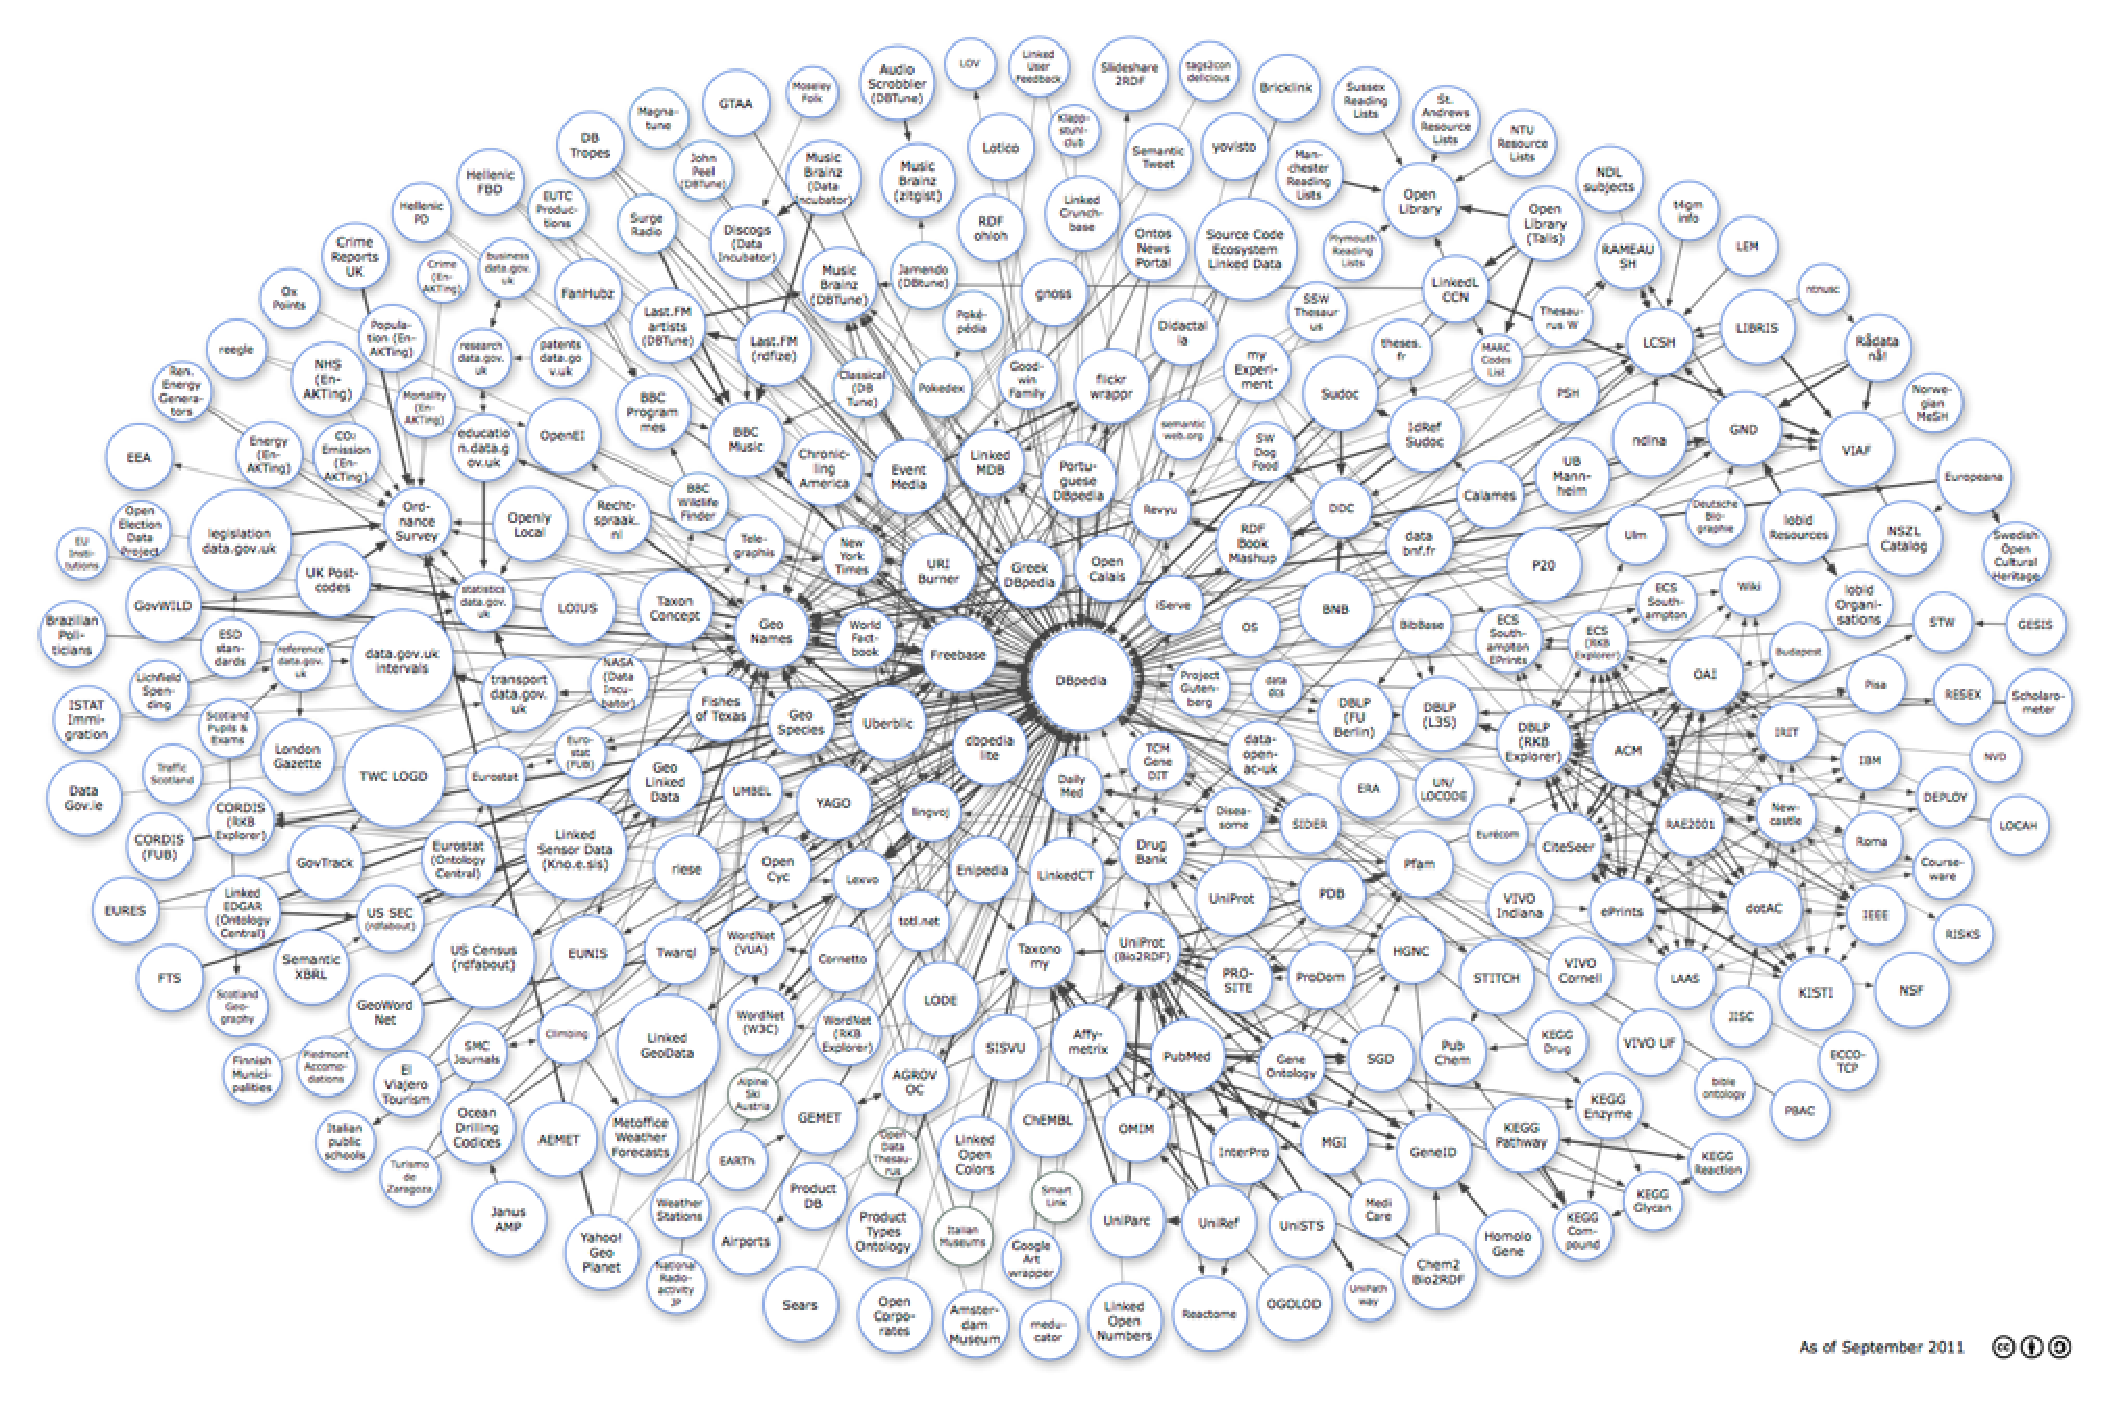
\includegraphics[width=10cm]{images/phd/lod-datasets_2011-09-19_1000px}
\caption{\textit{Linking Open Data cloud diagram, by Richard Cyganiak and Anja Jentzsch}.}
\label{fig:lod-cloud}
\end{figure}

Por otra parte, la información que se puede encontrar en la nueva \wod es tan variada como en la actual
web de documentos, a continuación algunos de los ejemplos de los datos que podemos encontrar, así:

\begin{itemize}
 \item Genéricos o de carácter transversal, candidatos ser reutilizados por cualquier conjunto de datos: DBPedia~\cite{Bizer:2009:D-C:1640541.1640848}, 
Freebase~\cite{freebase}, etc.
 \item Geográficos: Geonames~\cite{geonames}, OpenStreetMap~\cite{open-street-maps} o GeoLinkedData~\cite{SLHA11}.
 \item ``Government Data'': Data Gov UK, Datos.es, etc.
 \item Educación, Multimedia, Bibliográficos, Científicos, Médicos, ``Social Media'', etc., que se pueden encontrar clasificados
en la versión del diagrama de la nube de \lod bajo diferentes colores.
\end{itemize}

A la hora de unirse a la \wod hay que tener en cuenta varias consideraciones, además de proveer
datos enlazados se deben tener en cuenta unos principios relativos al diseño:

\begin{description}
 \item [Diseño de las \gls{URI}s.] Se busca que las URIs referencien a objetos reales y que se puedan obtener
descripciones a través de los protocolos propios de Internet, alineado directamente con el segundo principio de datos
enlazados y en este sentido hay que tener en cuenta varios aspectos: 
\begin{itemize}
 \item Uso de ``minting \gls{HTTP URI}s'': son URIs que están bajo el control del aquel que publica datos, es decir, utiliza
las URIs de su dominio para los datos y documentos.
\item ``Cool URIs''~\cite{Sauermann+2007a,bernerslee1998uri}: las URIs deben permanecer en el tiempo, en todo caso los usuarios las pueden cambiar, pero los identificadores
deberían permanecer inalterados. De la misma forma, se debe proveer un mecanismo para que a través de una misma URI se pueda
acceder a distinto contenido mediante negociación de contenido, extensiones, etc. 
\item ``Meaningful URIs'' vs ``ID based URIs''~\cite{uris-uk}: al igual que en el punto anterior nos encontramos ante la tesitura
de diseñar identificadores que se puedan recordar y con significado respecto a su contenido o bien utilizar
identificadores autogenerados. En cualquier caso, la decisión dependerá de la información a identificar, pero 
hay que tener presente este factor como clave en el diseño de la identificación de datos.
\end{itemize}
\item [Descripción de recursos con \gls{RDF}.] En este sentido se han establecido una serie de buenas prácticas y patrones
para describir los datos de los recursos susceptibles de publicación, ver Sección~\ref{metodologias}. Es importante seguir estas guías con el objeto de facilitar
su consulta a través de lenguajes como \gls{SPARQL}.
\item [Metainformación sobre los datos publicados.] No se trata sólo de publicar datos, ni de la apertura de las bases de datos
a la web, sino también de suministrar información sobre qué, cómo y dónde se puede acceder a estos datos. Para ello,
se debe atender a los siguientes criterios:
\begin{itemize}
 \item Usar vocabularios para describir el \dataset como \gls{voID}~\cite{void} o ``Semantic Sitemaps''\cite{Cyganiak08semanticsitemaps}.
 \item Añadir información sobre la procedencia~\cite{DBLP:conf/ipaw/HartigZ10,w3c-prov} de los datos (\provenance).
 \item Añadir información sobre la licencia~\cite{ld-licencias} de uso de los datos y los derechos de autoría, copia, distribución y modificación.
 \item Añadir información sobre la evolución temporal~\cite{ld-memento}, se puede conseguir mediante diferentes técnicas, incluyendo
la información en las URIs, en las descripciones RDF o mediante negociación de contenido.
\end{itemize}

\item [Seleccionar vocabularios a utilizar.] Existe un gran número de vocabularios~\cite{dcat-group} diseñados para describir
diversos tipos de información. La tendencia es reutilizar los vocabularios existentes~\cite{lod-stats} en la medida de lo posible, 
evitando re-modelar información ya descrita. Aunque existen catálogos de vocabularios, finalmente es la experiencia
y la consulta de otros \datasets la principal vía de información para seleccionar los vocabularios a reutilizar.
En general se atenderá a los siguientes factores: uso actual, mantenimiento, cobertura y expresividad.

\item [Enlazar con otros ``\datasets''.] Al igual que en el punto anterior no existe una forma estándar
de realizar este proceso, puede ser manual o automático, pero si que es necesario fijar la atención en la semántica del enlace y seleccionar aquellos recursos que sean
de mayor uso para asegurar de nuevo la coherencia de nuestros datos y su difusión.

\item [Publicar los datos.] Una vez determinados los datos a publicar, los cuales se han transformado y enlazado (si resultara oportuno), es
necesario proceder a su publicación de forma estandarizada mediante la aplicación de ciertos patrones definidos y teniendo en cuenta
si los datos son o no dinámicos, la criticidad, el esfuerzo de duplicar bases de datos, los formatos que van a ser soportados,
la exposición mediante servicios de consulta, el uso de un API, etc.
\item [Consumir datos publicados.] Este proceso conlleva la explotación de los datos disponibles tanto para generar
nuevos servicios de negocio comerciales o simplemente para consultar la información que se haya publicada y que se 
puede enriquecer con el universo de los demás \textit{datasets} publicados.
\item [Difundir los datos publicados.] Aunque no se trata de una acción o requisito funcional, el éxito de un conjunto
de datos publicados dependerá en buena medida, además de su calidad~\cite{ld-quality} y facilidad de acceso, de la difusión que se realice
sobre su uso y capacidad. Para ello, existen diversos catálogos~\cite{TummarelloDO07} y herramientas de indexado, por ejemplo
\textit{thedatahub.org}, \textit{prefix.cc}, etc., en los cuales se puede incluir los datos publicados para que así, terceros 
los puedan consumir. La información de difusión deberá incluir aspectos relativos sobre cómo acceder a los datos, qué datos están publicados, el tipo de licencia, etc., para asegurar la confianza necesaria en los usuarios finales.

\end{description}

Como se ha reseñado en los puntos anteriores, pese a que existen patrones, recetas y métodos de producción, publicación y consumo de datos
es decisión del responsable la selección de los mismos. Si bien la flexibilidad de actuación queda patente y beneficia
la publicación masiva de datos, lleva consigo una desventaja, que reside en la posibilidad de errar en ciertos puntos provocando
una baja calidad en los datos. Para ello, tal y como se expone en la siguiente sección existen diversos esfuerzos para poner en común
estas guías bajo una metodología especificando las actividades, participantes, herramientas y productos de entrada y salida
en cada una de las partes del proceso. En nuestro caso, esta situación es de especial relevancia para poder evaluar las ventajas
de uso de datos enlazados, en contraposición con la actual situación de manejo de datos en el campo de la contratación pública
electrónica.

\subsection{Metodologías y Buenas Prácticas}\label{metodologias}
En las anteriores secciones se han presentando las diferentes iniciativas entorno a datos enlazados en un contexto
general, pero teniendo presentes las necesidades de la administración pública electrónica. Han quedado patentes las necesidades,
ventajas y algunas desventajas del uso de esta iniciativa para los procesos de producción, publicación y consumo de datos. Si 
bien existen muchas guías y principios de diseño que se pueden extraer a través de la literatura, es conveniente repasar
los enfoques que se están desarrollando para realizar una guía sobre cómo se deben aplicar los conceptos de  \linkeddata, \opendata, \ogd, \lod, etc., 
para ello existen diferentes guías e incluso plataformas que aglutinan una serie de características de interés que a continuación se listan, 
repasando las más destacadas.

\begin{itemize}
 \item \textit{Linked Data Design Considerations} del libro \textit{Linked Data: Evolving the Web into a Global Data Space}~\cite{Heath_Bizer_2011}.
 \item \textit{Linked Data Patterns}~\cite{linked-data-patterns}.
 \item \textit{Best Practices}~\cite{best-gld,Berr08} del grupo de trabajo del \gls{W3C} \textit{Government Linked Data First \gls{F2F} June 29-30, 2011}~\cite{gld-group}.
 \item \textit{Linked Data Cookbook}~\cite{linked-data-cookbook} del grupo de trabajo del W3C \textit{Government Linked Data Working Group}~\cite{gld-group}.
 \item \textit{Government Linked Data-Life Cycle}~\cite{gld-lifecycle} del grupo de trabajo del W3C \textit{Government Linked Data Working Group}.
 \item \textit{Publishing Open Government Data}~\cite{publishing-ogd} borrador de trabajo del W3C.
 \item \textit{LOD2 Stack}~\cite{lod2-stack} del proyecto europeo \textit{LOD2}~\cite{lod2-project}.
 \item \textit{Toward a Basic Profile for Linked Data}~\cite{basic-profile-w3c,basic-profile-ibm} de IBM.
 \item Metodología~\cite{DBLP:conf/i-semantics/Cifuentes-SilvaSG11,methodologyCaepia2011} propuesta por la Universidad de Oviedo en el ámbito de la Biblioteca del Congreso de Chile.
 \item \textit{Talis Platform}~\cite{talis}.  
 \item \textit{Linked Open Data: The Essentials}~\cite{Bauer2012}.
\item Documentación específica de cada país e incluso región para el despliegue de \opendata.
\end{itemize}

El objetivo de estas guías es definir unas directrices sobre cómo publicar los datos para obtener una \wod de calidad. Además y en 
esta misma línea se están organizando continuamente conferencias, talleres, etc., específicos dentro de los grandes eventos científicos
para divulgar las actividades relacionadas con \linkeddata, como por ejemplo \textit{Consuming Linking Open Data}~\cite{cold} (\gls{COLD}), 
\textit{Linked Data On the Web}~\cite{ldow} (\gls{LDOW}), \textit{Social Data On the Web}~\cite{sdow} (\gls{SDOW}) o \textit{Linked Enterprise Data Patterns}~\cite{linked-enterprise-data-patterns} que sirven 
como concentrador de las actividades que se están realizando en este ámbito y que abordan los principales problemas 
que aparecen en este entorno emergente.

\subsubsection{\textit{Linked Data Design Considerations}}\label{linked-data-design-issues}
En el libro~\cite{Heath_Bizer_2011} realizado por Chris Bizer (investigador en la Freie Universitat de Berlin, Alemania y creador de la DBPedia) y 
por Tom Heath (uno de los investigadores principales de la plataforma Talis~\cite{talis}) se ponen de manifiesto una serie de consideraciones, ver Tabla~\ref{table:linkeddata-design-book}
de diseño a tener en cuenta cuando se pretende desplegar una plataforma de datos enlazados. 


\begin{longtable}[c]{|l|p{7cm}|p{8cm}|} 

\hline

  \textbf{ID} & \textbf{Directriz} &  \textbf{Descripción} \\\hline

\endhead
   1& \multicolumn{2}{|c|}{\textbf{\textit{Using URIs as Names for Things}}}\\ \hline
   1.1 &  \textit{Minting \gls{HTTP URI}s} & Las URIs deben permitir acceder a los recursos que nombran. Uso del schema HTTP. \\ \hline
   1.2 &  \textit{Use of Cool URIs} &  Las URIs deben seguir unos criterios de diseño que permitan y animen a terceros su uso.\\ \hline
   1.3 &  \textit{Keep out of namespaces you do not control} &  Las URIs de los recursos deben pertenecer a un dominio sobre el que se tenga control.\\ \hline
   1.4 &  \textit{Abstract away from implementation details} & Las URIs no incluyen detalles de implementación como el formato del recurso. \\ \hline
   1.5 &  \textit{Use Natural Keys within URIs} &  Para asegurar que las URIs son únicas se utiliza una clave primaria o ID para identificar recursos.\\ \hline
   1.6 &  \textit{Hash URIs} &  La concatenación de identificadores en el URI se realiza utilizando \# como separador final del recurso.\\ \hline
   1.7 &  \textit{Slash URIs} &  Igual que en el caso anterior pero utilizando $/$. \\ \hline
   2&\multicolumn{2}{|c|}{\textbf{\textit{Describing Things with RDF}}}\\ \hline
   2.1 &  \textit{\gls{RDF} resources} & Cuando se accede a un recurso a través de un \gls{URI} se debe proveer información útil. \\ \hline
   2.2 &  \textit{Literal Triples and Outgoing Links} & El sujeto de la información en RDF es siempre el URI del recurso que se está describiendo. \\ \hline
   2.3 &  \textit{Incoming Links} & Proveer enlaces a otros recursos para hacer los datos navegables. \\ \hline
   2.4 &  \textit{Triples that Describe Related Resources} & Describir parcialmente los recursos que son enlazados desde el actual. \\ \hline
   2.5 &  \textit{Triples that Describe the Description} & Añadir metainformación sobre los propios recursos como licencia. \\ \hline
  3&\multicolumn{2}{|c|}{\textbf{\textit{Publishing Data about Data}}}\\ \hline
   3.1 &  \textit{Describing a Data Set} & Añadir metainformación sobre el conjunto de datos que se está publicando. \\ \hline
   3.2 &  \textit{Use of Semantic Sitemaps} & Utilizar la extensión de \textit{Sitemap} para describir los datos proveyendo capacidades nuevas para los buscadores. \\ \hline
   3.3 &  \textit{Use of voiD Descriptions} & Utilizar el vocabulario voiD (the Vocabulary of Interlinked Datasets) para la metainformación de los datos. Es considerado el estándar de facto. \\ \hline
   3.4 &  \textit{Provenance Metadata} & Añadir información sobre la procedencia de los datos. Capacidades de monitorización y evolución en el tiempo. \\ \hline
   3.5 &  \textit{Licenses, Waivers and Norms for Data} & Incluir información sobre el uso posible de los datos a través de una licencia. \\ \hline
   3.6 &  \textit{Non-copyrightable Material} & $\approxeq$ \\ \hline
   4&\multicolumn{2}{|c|}{\textbf{\textit{Choosing and Using Vocabularies to Describe Data}}}\\ \hline
   4.1 &  \textit{\gls{SKOS}, RDFS and \gls{OWL}} &  Modelar la información de los datos de acuerdo a un vocabulario estándar. Proveer un modelo formal para los datos.\\ \hline
   4.2 &  \textit{Annotations in RDFS} &  Usar las anotaciones \texttt{rdfs:label} y \texttt{rdfs:comment} en las descripciones de RDF.\\ \hline
   4.3 &  \textit{Relating Classes and Properties} &  Relacionar los recursos en RDF mediante propiedades de RDFS, SKOS, etc.: \texttt{rdfs:subClassOf}, \texttt{skos:related}, etc.  \\ \hline
   4.4 &  \textit{Reusing Existing Terms} & Reutilizar las definiciones ya concebidas en los vocabularios existentes de los distintos dominios como: Dublin Core, FOAF, etc. \\ \hline
   4.5 &  \textit{Selecting Vocabularies} & Seleccionar los vocabularios a reutilizar teniendo en cuenta: \textit{Usage and uptake}, \textit{Maintenance and governance}, \textit{Coverage} y \textit{Expressivity}.\\ \hline
   4.6 &  \textit{Defining Terms} &  Si los vocabularios existentes no cubren las necesidades de nuestros datos, definir nuevos términos.\\ \hline
   5&\multicolumn{2}{|c|}{\textbf{\textit{Making Links with RDF}}}\\ \hline
   5.1 &  \textit{Publishing Incoming and Outgoing Links} &  Publicar un volcado de los datos en RDF.\\ \hline
   5.2 &  \textit{Making Links with External Data Sources} &  Reutilizar y enriquecer las descripciones en RDF con otras ya existentes asegurando que existen.\\ \hline
   5.3 &  \textit{Choosing External Linking Targets} & Los enlaces a datos externos deben cumplir que sean referenciables mediante un URI y deberían ser reutilizados por otros.\\ \hline
   5.4 &  \textit{Choosing Predicates for Linking} & Similar al punto $22$.\\ \hline
   5.5 &  \textit{Setting RDF Links Manually} & Incluir enlaces en las descripciones en RDF mediante edición manual (si de forma automática no es fiable).\\ \hline
   5.6 &  \textit{Auto-generating RDF Links} & Incluir enlaces las descripciones en RDF de forma automática. Uso de herramientas de reconciliación de entidades: SILK, LIMES, etc.\\ \hline
   5.7 &  \textit{Key-based Approaches} & Los enlaces se realizan mediante búsqueda de recursos con palabras claves.\\ \hline
   5.8 &  \textit{Similarity-based Approaches} & Los enlaces se realizan mediante búsqueda de recursos de acuerdo a una estructura.\\ \hline
  6&\multicolumn{2}{|c|}{\textbf{\textit{Recipes for Publishing Linked Data}}}\\ \hline
   6.1 &  \textit{Linked Data Publishing Patterns} & Establecer el modelo para ofrecer los datos.\\ \hline
   6.2 &  \textit{From Queryable Structured Data to Linked Data} & Exportar una base de datos relacional mediante un mapeador a RDF.\\ \hline
   6.3 &  \textit{From Static Structured Data to Linked Data} & Transformar datos estáticos a RDF. Por ejemplo: CSV, MSExcel, etc.\\ \hline
   6.4 &  \textit{From Text Documents to Linked Data} & Extraer los datos RDF de documentos de texto.\\ \hline
   6.5 &  \textit{Data Volume: How much data needs to be served?} & Dependiendo de la cantidad de datos definir qué datos y cantidad se pueden exportar.\\ \hline
   6.6 &  \textit{Data Dynamism: How often does the data change?} & Dependiendo de los cambios en los datos definir qué patrón (\textit{from}) se adapta mejor a la exportación de los datos.\\ \hline
   6.7 &  \textit{Serving Linked Data as Static RDF/XML Files} & Publicar los ficheros en RDF en un servidor web. Forma más sencilla.\\ \hline
   6.8 &  \textit{Hosting and Naming Static RDF Files} & Utilizar una convención de nombrado y negociación de contenido para los ficheros en RDF. Reglas de reescritura en servidor web.\\ \hline
   6.9 &  \textit{Server-Side Configuration: \gls{MIME} Types} & Servir el contenido apropiado de acuerdo a los tipos MIME.\\ \hline
   6.10 &  \textit{Making RDF Discoverable from \gls{HTML}} & Permitir que desde HTML se pueda reutilizar las descripciones en RDF.\\ \hline
   6.11 &  \textit{Serving Linked Data as RDF Embedded in HTML Files} & Enriquecer HTML con las descripciones en RDF. Por ejemplo con RDFa.\\ \hline
   6.12 &  \textit{Serving RDF and HTML with Custom Server-Side Scripts} & Generación bajo demanda de RDF en el servidor.\\ \hline
   6.13 &  \textit{Serving Linked Data from Relational Databases} & Generación bajo demanda de RDF en el servidor mapeando a una base de datos.\\ \hline
   6.14 &  \textit{Serving Linked Data from RDF Triple Stores} & Utilizar las capacidades de un triple-store para ofrecer RDF.\\ \hline
   6.15 &  \textit{Serving Linked Data by Wrapping Existing Application or Web \gls{API}s} & Exportar los datos de las aplicaciones web existentes como RDF.\\ \hline
   6.16 &  \textit{Testing and Debugging Linked Data} & Utilizar herramientas para verificar que se cumple con los principios de \linkeddata y de la publicación de datos.\\ \hline
   7&\multicolumn{2}{|c|}{\textbf{\textit{Architecture of Linked Data Applications}}}\\ \hline
   7.1 &  \textit{The Crawling Pattern} & Se navega por los recursos RDF con el objeto de extraer los datos para proveer servicios y datos a una capa superior.\\ \hline
   7.2 &  \textit{The On-The-Fly Dereferencing Pattern} & El patrón de los navegadores de \linkeddata que extraen la información de los recursos en el momento en el que se necesita.\\ \hline
   7.3 &  \textit{The Query Federation Pattern} & Se crean consultas complejas ejecutadas sobre varias fuentes de datos que se presentan al usuario dentro de una aplicación.\\ \hline
 
\hline
\caption{Consideraciones de Diseño \linkeddata}\label{table:linkeddata-design-book}\\    
\end{longtable}

Como se puede comprobar, en esta lista residen una serie de consideraciones a valorar en relación con la producción, publicación y consumo de datos
enlazados. La implementación o el uso que se realice de cada uno de estos puntos depende de la estrategia seguida por la persona o institución
implicada en el proceso de ofrecer sus datos bajo la iniciativa \linkeddata. Finalmente y tras aplicar estos principios se puede utilizar
el siguiente \textit{checklist}, es similar al utilizado para añadir un conjunto de datos a la iniciativa \gls{LOD} Cloud,
 para verificar, ver Tabla~\ref{table:linkeddata-check-list}, si se han 
aplicado de forma correcta los principios de diseño propuestos por los autores y en consecuencia de \linkeddata.


\begin{longtable}[c]{|l|p{7cm}|p{8cm}|} 

\hline

  \textbf{ID} & \textbf{Punto a cumplir} &  \textbf{Descripción} \\\hline

\endhead
   1 &  \textit{Does your data set links to other data sets?} & Existen enlaces externos desde las descripciones en RDF a otros externos que conformen un grafo global .\\ \hline
   2 &  \textit{Do you provide provenance metadata?} &  Los datos disponen de información sobre su procedencia.\\ \hline
   3 &  \textit{Do you provide licensing metadata?} &  Se establecen las restricciones necesarias sobre el uso de los datos.\\ \hline
   4 &  \textit{Do you use terms from widely deployed vocabularies?} & Las descripciones en \gls{RDF} se basan en reutilizar clases y propiedades ya existentes y aplicadas ampliamente. \\ \hline
   5 &  \textit{Are the URIs of proprietary vocabulary terms dereferenceable?} & Las clases y propiedades definidas particularmente son referenciables. \\ \hline
   6 &  \textit{Do you map proprietary vocabulary terms to other vocabularies?} &  Las clases y propiedades definidas se basan y relacionan con otras ya existentes y aplicadas ampliamente.\\ \hline
   7 &  \textit{Do you provide data set-level metadata?} &  Se ofrece metainformación sobre el conjunto de datos en general\\ \hline
   8 &  \textit{Do you refer to additional access methods?} &  Además del uso de \gls{URI}s para referenciar los datos se proveen otros servicios como un \textit{endpoint} de SPARQL.\\ \hline

\hline
\caption{\textit{Checklist} \linkeddata}\label{table:linkeddata-check-list}\\    
\end{longtable}

\begin{figure}[!htb]
\centering
	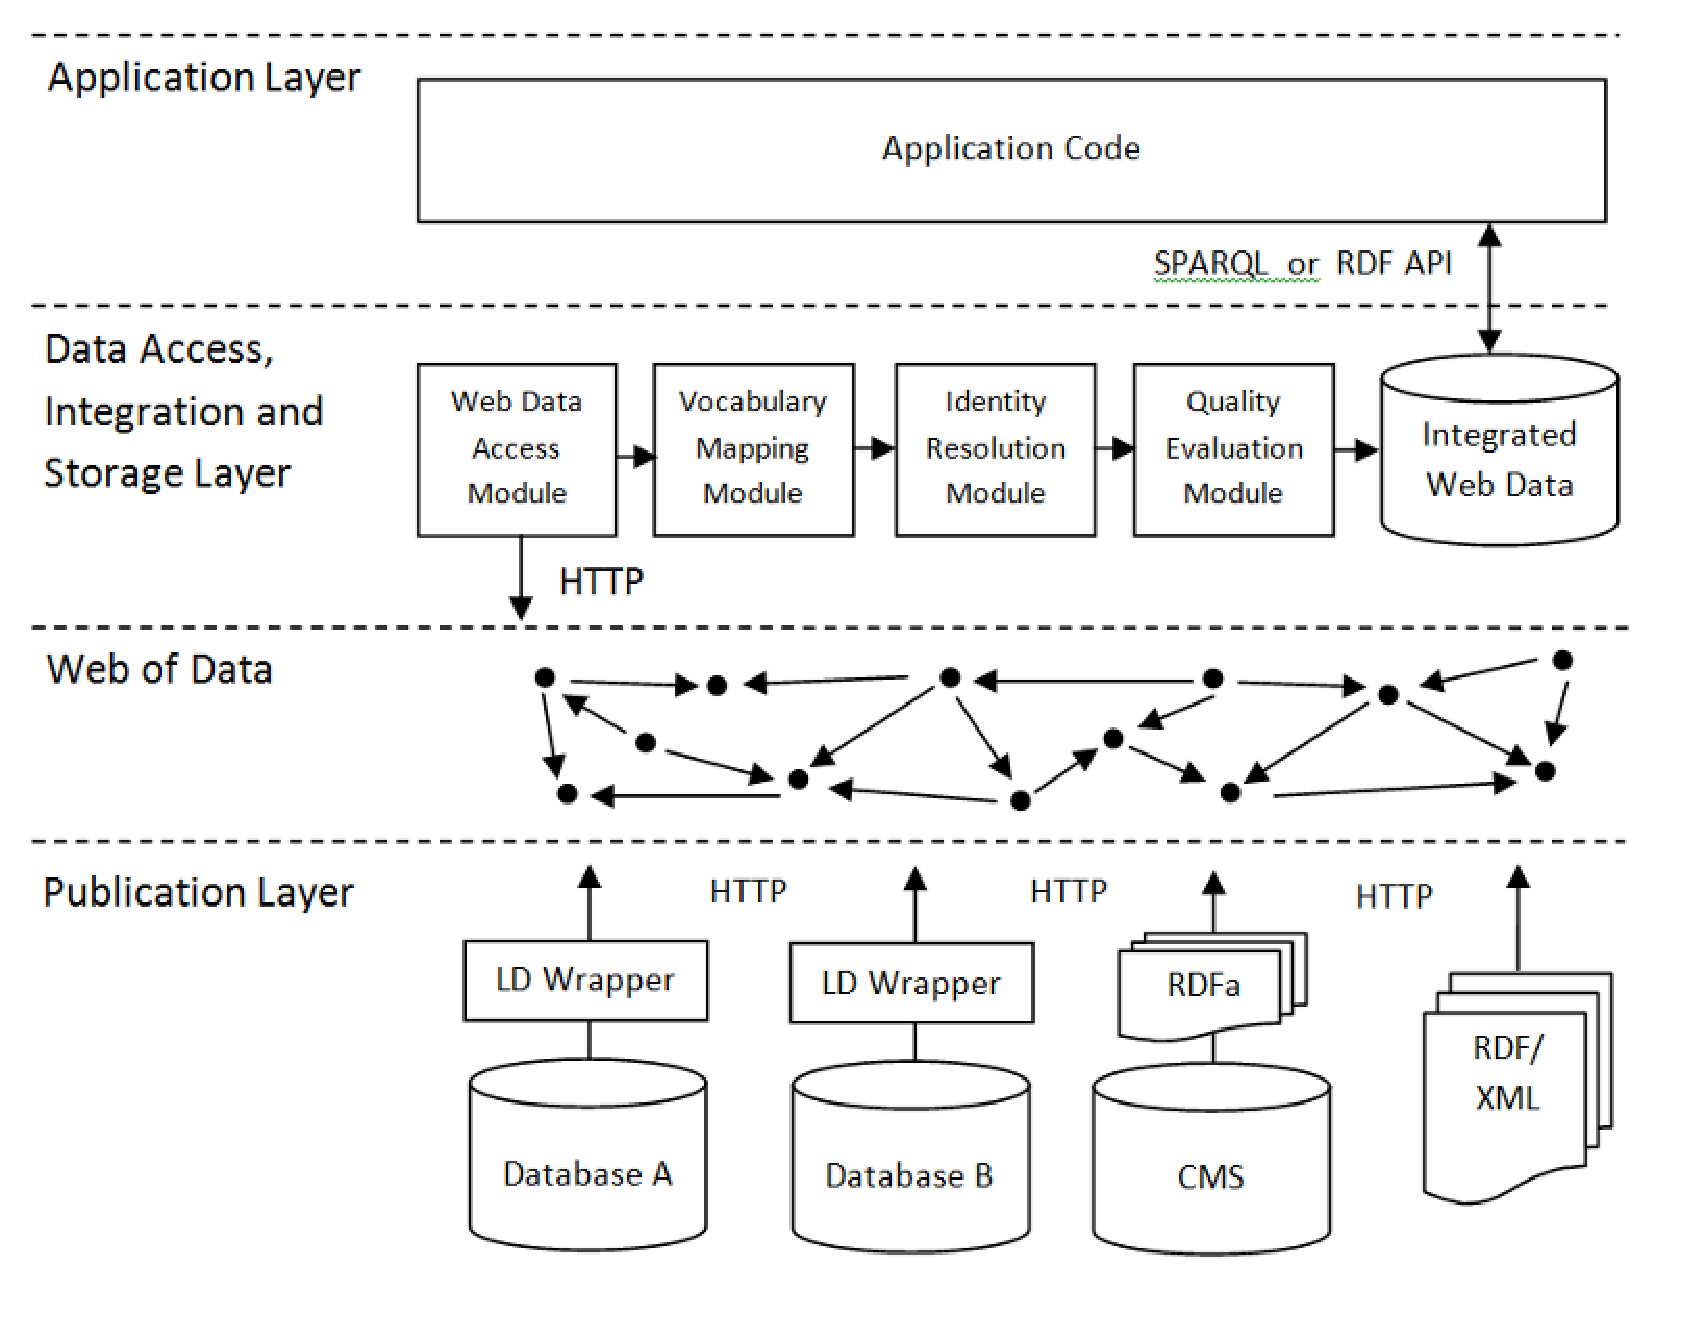
\includegraphics[width=10cm]{images/phd/Consumingarchitecture1_small}
\caption{\textit{Linked Data Publishing Options and Workflows} (extraída de \textit{Linked Data Design Considerations}).}
\label{fig:patterns-production}
\end{figure}

En conclusión, en este libro se ofrece una guía práctica y didáctica de los pasos a seguir para la aplicación
de la iniciativa de \linkeddata de forma correcta, asegurando las ventajas en los datos enlazados, minimizando las desventajas
y proveyendo un entorno para la generación de servicios de alto valor y calidad. 
Como podemos observar tanto las directrices de la Tabla~\ref{table:linkeddata-design-book}, como
los puntos a cumplir de la Tabla~\ref{table:linkeddata-check-list}, se pueden englobar en tres grandes procesos: producción,
publicación y consumo de \linkeddata. Especialmente hay que destacar los enfoques para la producción de \linkeddata desde
fuentes de datos ya existentes, ver Figura~\ref{fig:patterns-production} y Figura~\ref{fig:patterns-consum}.

\begin{figure}[!htb]
\centering
	\includegraphics[width=10cm]{images/phd/D2RServerArchitecture}
\caption{Architectura de D2R Server.}
\label{fig:patterns-consum}
\end{figure}


\subsubsection{\textit{Linked Data Patterns}}\label{linked-data-patterns}
Con el objetivo de proveer una forma estándar de transformar los datos
siguiendo la iniciativa de \linkeddata y disponer de unos criterios y soluciones estándar
para modelar, publicar y consumir datos, se han publicado una serie de patrones~\cite{linked-data-patterns} que resuelven
los problemas más comunes que se pueden encontrar. A continuación, ver Tabla~\ref{table:linkeddata-patterns}, se describen
algunos de los propuestos por los autores:


\begin{longtable}[c]{|l|p{7cm}|p{8cm}|} 

\hline

  \textbf{ID} & \textbf{Patrón} &  \textbf{Pregunta} \\\hline

\endhead
   1& \multicolumn{2}{|c|}{\textbf{\textit{Identifier Patterns}}}\\ \hline
  1.1 &  \textit{Hierarchical URIs} & \textit{How should URIs be assigned to a group of resources that form a natural hierarchy?}\\ \hline
  1.2 &  \textit{Literal Keys} & \textit{How do we publish non-global identifiers in \gls{RDF}?} \\ \hline
  1.3 &  \textit{Natural Keys} &  \textit{How can we create unique URIs from data that already has unique identifiers?} \\ \hline
  1.4 &  \textit{Patterned URIs} & \textit{How can we create more hackable, human-readable URIs?} \\ \hline
  1.5 &  \textit{Proxy URIs} & \textit{How do we deal with lack of standard identifiers for third-party resources?} \\ \hline
  1.6 &  \textit{Shared Keys} & \textit{How do we simplify the inter-linking of datasets?} \\ \hline
  1.7 &  \textit{URL Slug} &  \textit{How can we create \gls{URL}s from arbitrary text or keywords?} \\ \hline    
    2& \multicolumn{2}{|c|}{\textbf{\textit{Modelling Patterns}}}\\ \hline
  2.1 &  \textit{Custom Datatype} &  \textit{A data model contains structured values that don't correspond to one of the pre-existing \gls{XML Schema} datatypes.} \\ \hline    
  2.2 &  \textit{Index Resources} &  \textit{How can ordered collections or indexes be published as RDF?}  \\ \hline    
  2.3 &  \textit{Label Everything} & \textit{How can we ensure that every resource has a basic human-readable name?} \\ \hline     
  2.4 &  \textit{Link Not Label} &  \textit{How do we model a dataset to maximise benefits of a graph based model?} \\ \hline    
  2.5 &  \textit{Multi-Lingual Literal} & \textit{How can internationalized text be expressed in RDF? }\\ \hline    
  2.6 &  \textit{N-Ary Relation} & \textit{How can a complex relation, involving several resources, be modelled as RDF? }\\ \hline    
  2.7 &  \textit{Ordered List} &  \textit{How do we specify an ordering over a collection of resources?} \\ \hline     
  2.8 &  \textit{Ordering Relation} & \textit{How can we specify an ordering relationship between two or more resources?} \\ \hline     
  2.9 &  \textit{Preferred Label} &  \textit{How can a simple unambiguous label be provided for a resource? }\\ \hline    
  2.10 &  \textit{Qualified Relation} &  \textit{How can we describe or qualify a relationship between two resources?} \\ \hline   
  2.11 &  \textit{Reified Statement} &  \textit{How can we make statements about statements?} \\ \hline    
  2.12 &  \textit{Topic Relation} &  \textit{How can a web page or document be associated with a resource?} \\ \hline      
  2.13 &  \textit{Typed Literal} &  \textit{How can a datatype be associated with an RDF literal?} \\ \hline        
    3& \multicolumn{2}{|c|}{\textbf{\textit{Publishing Patterns}}}\\ \hline
  3.1 &  \textit{Annotation} &  \textit{How can data about third-party resources be published as part of a dataset?}  \\ \hline    
  3.2 &  \textit{Autodiscovery} &   \textit{How can people find the underlying linked data for a given web page?}  \\ \hline    
  3.3 &  \textit{Document Type} & \textit{How can some context be provided about a set of RDF triples published to the web?} \\ \hline     
  3.4 &  \textit{Edit Trail} &  \textit{How can people be encouraged to improve or fix up open data?} \\ \hline    
  3.5 &  \textit{Embedded Metadata} &  \textit{How do we add structured data to an existing document or file?} \\ \hline    
  3.6 &  \textit{Equivalence Links} &  \textit{How do we indicate that different \gls{URI}s refer to the same resource or concept?} \\ \hline    
  3.7 &  \textit{Link Base} &  \textit{How can outbound links from a dataset be managed separately from the core data?} \\ \hline     
  3.8 &  \textit{Materialize Inferences} &  \textit{How can data be published for use by clients with limited reasoning capabilities?} \\ \hline     
  3.9 &  \textit{Named Graphs} & \textit{How do we organize and annotate a set of RDF statements?} \\ \hline    
  3.10 &  \textit{Primary Topic Autodiscovery} & \textit{How can people identify the principal subject of a given web page?}  \\ \hline    
  3.11 &  \textit{Progressive Enrichment} &  How can the quality of data or a data model be improved over time? \\ \hline      
  3.12 &  \textit{See Also} & \textit{How can RDF documents be linked together to allow crawlers and user agents to navigate between them?} \\ \hline    
        4& \multicolumn{2}{|c|}{\textbf{\textit{Application Patterns}}}\\ \hline
  4.1 &  \textit{Assertion Query} & \textit{How can a dataset be tested for known patterns?} \\ \hline    
  4.2 &  \textit{Blackboard} &  \textit{How can the task of compiling or constructing a dataset be divided up into smaller tasks?}\\ \hline    
  4.3 &  \textit{Bounded Description} & \textit{How can we generate a useful default description of a resource without having to enumerate all the properties or relations that are of interest?} \\ \hline     
  4.4 &  \textit{Composite Descriptions} &  \textit{How do we declare the underlying dataset for a page involving custom subsets or views of the data?}\\ \hline    
  4.5 &  \textit{Follow Your Nose} &  \textit{How do we find additional relevant data from the web?} \\ \hline    
  4.6 &  \textit{Missing Isn't Broken} &  \textit{How do we handle the potentially messy or incomplete data we use from the web?} \\ \hline    
  4.7 &  \textit{Parallel Loading} &  \textit{How can we reduce loading times for a web-accessible triple store?} \\ \hline     
  4.8 &  \textit{Parallel Retrieval} & \textit{ How can we improve performance of an application dynamically retrieving Linked Data?} \\ \hline     
  4.9 &  \textit{Resource Caching} &  \textit{How can an application that relies on loading data be more tolerant of network failures and/or reduce use of bandwidth} \\ \hline    
  4.10 &  \textit{Schema Annotation} & \textit{How can application-specific processing rules be externalized?} \\ \hline    
  4.11 &  \textit{Smushing} &  \textit{How do we merge data about resources that may not be consistently identified?} \\ \hline
  4.12 &  \textit{Transformation Query} & \textit{How can we normalize or transform some RDF data so that it conforms to a preferred model?} \\ \hline        
 
\hline
\caption{\textit{Linked Data Patterns}}\label{table:linkeddata-patterns}\\    
\end{longtable}

Al igual que en el caso anterior, en estos patrones se ofrecen una serie de guías para resolver problemas comunes
que surgen en el momento de producir, publicar y consumir datos enlazados. Suponen una información muy valiosa, ya que
permiten homogeneizar la creación de datos enlazados de tal forma que si una persona u organización asegura que ha 
seguido estos principios, se pueden construir aplicaciones que sepan qué tipo de datos se van encontrar y cómo, disminuyendo
así el coste de reutilización de datos provenientes de terceros y asegurar la calidad de los mismos.

\subsubsection{\textit{Best Practices} del W3C}
Se trata de una serie de documentos y buenas prácticas~\cite{best-gld} dentro del 
grupo de trabajo del \gls{W3C} \textit{Government Linked Data Working Group}~\cite{gld-group} cuya actividad se lanzó
 en el \textit{Face 2 Face} de junio de 2011 y que consta de los siguientes objetivos:

\begin{itemize}
 \item \textit{The overarching objective is to provide best practices and guidance to create of high quality, re-usable Linked Open Data (LOD)}.
 \item \textit{Description of the full life cycle of a Government Linked Data project, starting with identification of suitable data sets, procurement, modeling, vocabulary selection, through publication and ongoing maintenance.}
 \item \textit{Definition of known, proven steps to create and maintain government data sets using Linked Data principles.}
  \item \textit{Guidance in explaining the value proposition for LOD to stakeholders, managers and executives.}
  \item \textit{Assist the Working Group in later stages of the Standards Process, in order to solicit feedback, use cases, etc.}
\end{itemize}

Como grupo de trabajo su esfuerzo se centrará en cumplir los objetivos establecidos a través de la consecución de materiales como 
recomendaciones, notas, etc., en los siguientes ámbitos:
\begin{enumerate}
 \item  \textit{Procurement.}
 \item  \textit{Vocabulary Selection.}
 \item \textit{URI Construction.}
   \item \textit{Versioning.}
   \item \textit{Stability.}
   \item \textit{Legacy Data.}
   \item \textit{Cookbook.} 
\end{enumerate}

Evidentemente y teniendo en cuenta los participantes en esta actividad, está claro que los puntos de actuación
seleccionados son claramente estratégicos para la iniciativa de \linkeddata y es por ello que aunque
los resultados están en una etapa previa, es conveniente sumamente atento a sus resultados con el doble objetivo
de por una parte aplicarlos a futuros proyectos y por otra parte realimentar el esfuerzo realizado por sus participantes.

\subsubsection{\textit{Linked Data Cookbook} del W3C}\label{linked-data-cookbook}
Uno de los esfuerzos de la actividad comentada en la sección anterior, consiste
en la elaboración de un libro de buenas prácticas~\cite{linked-data-cookbook} en cuanto a la producción, publicación y consumo de 
datos enlazados. Para ello se recopilarán las prácticas más comunes
desde el punto de vista de la ingeniería que faciliten la adopción de \linkeddata en 
diferentes entornos, asegurando una calidad y previniendo que el uso de datos enlazados
no sea sinónimo de depuración.

Con carácter previo se han fijado una serie de pasos que se han de seguir para desplegar
una infraestructura de datos enlazados acompañada de una serie de prácticas que aseguren
la calidad y el proceso de adopción. Esta iniciativa es compatible con las buenas prácticas
vista en las Secciones~\ref{linked-data-design-issues} y~\ref{linked-data-patterns} y además
ofrece una buena guía de todos los puntos que hay que tener en cuenta: diseño de URIs, vocabularios
a reutilizar, herramientas, etc. Actualmente estas prácticas se están desarrollando y 
se dividen en $7$ pasos que se presentan en la Tabla~\ref{table:linkeddata-practices}.


\begin{longtable}[c]{|l|p{7cm}|p{8cm}|} 

\hline

  \textbf{ID} & \textbf{Práctica} & \textbf{Descripción} \\\hline

\endhead
  1 &  \textit{Model the Data} & \textit{Identify, Model, Name and Test.}\\ \hline
  2 &  \textit{Name things with \gls{URI}s} & \textit{Following a name convention of current guides.} \\ \hline
  3 &  \textit{Re-use vocabularies whenever possible} &   \textit{Any given Linked Data set may include terms from an existing and widely used vocabulary.} \\ \hline
  4 &  \textit{Publish human and machine readable descriptions} & \textit{Self-describing data suggests that ''information about the encodings used for each representation is provided explicitly within the representation``}.  \\ \hline
  5 &  \textit{Convert data to \gls{RDF}} & N/A \\ \hline
  6 &  \textit{Specify an appropriate license} & N/A \\ \hline
  7 &  \textit{Announce the new Linked Data Set(s) } &  N/A  \\ \hline    
 
\hline
\caption{\textit{The 7 Best Practices for Producing Linked Data.}}\label{table:linkeddata-practices}\\    
\end{longtable}


\subsubsection{\textit{Government Linked Data-Life Cycle}}\label{gld}
Siguiendo con las actividades que se desarrollan en este grupo de trabajo del W3C sobre datos enlazados
en el entorno de la administración pública electrónica, se han identificado los siguientes ciclos de vida~\cite{gld-lifecycle} propuestos
por diversos autores:

\begin{itemize}
 \item Bernadette Hyland, ver Figura~\ref{fig:hyland}. 

\begin{figure}[!htb]
\centering
	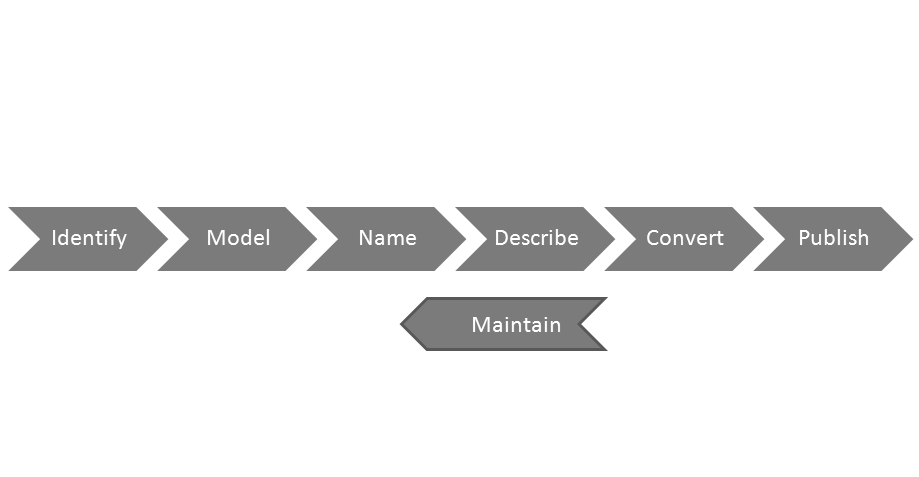
\includegraphics[width=14cm]{images/phd/Hyland}
\caption{\textit{Linked Data Lifecycle by B. Hyland}.}
\label{fig:hyland}
\end{figure}


 \item Michael Hausenblas, ver Figura~\ref{fig:hausenblas}.

\begin{figure}[!htb]
\centering
	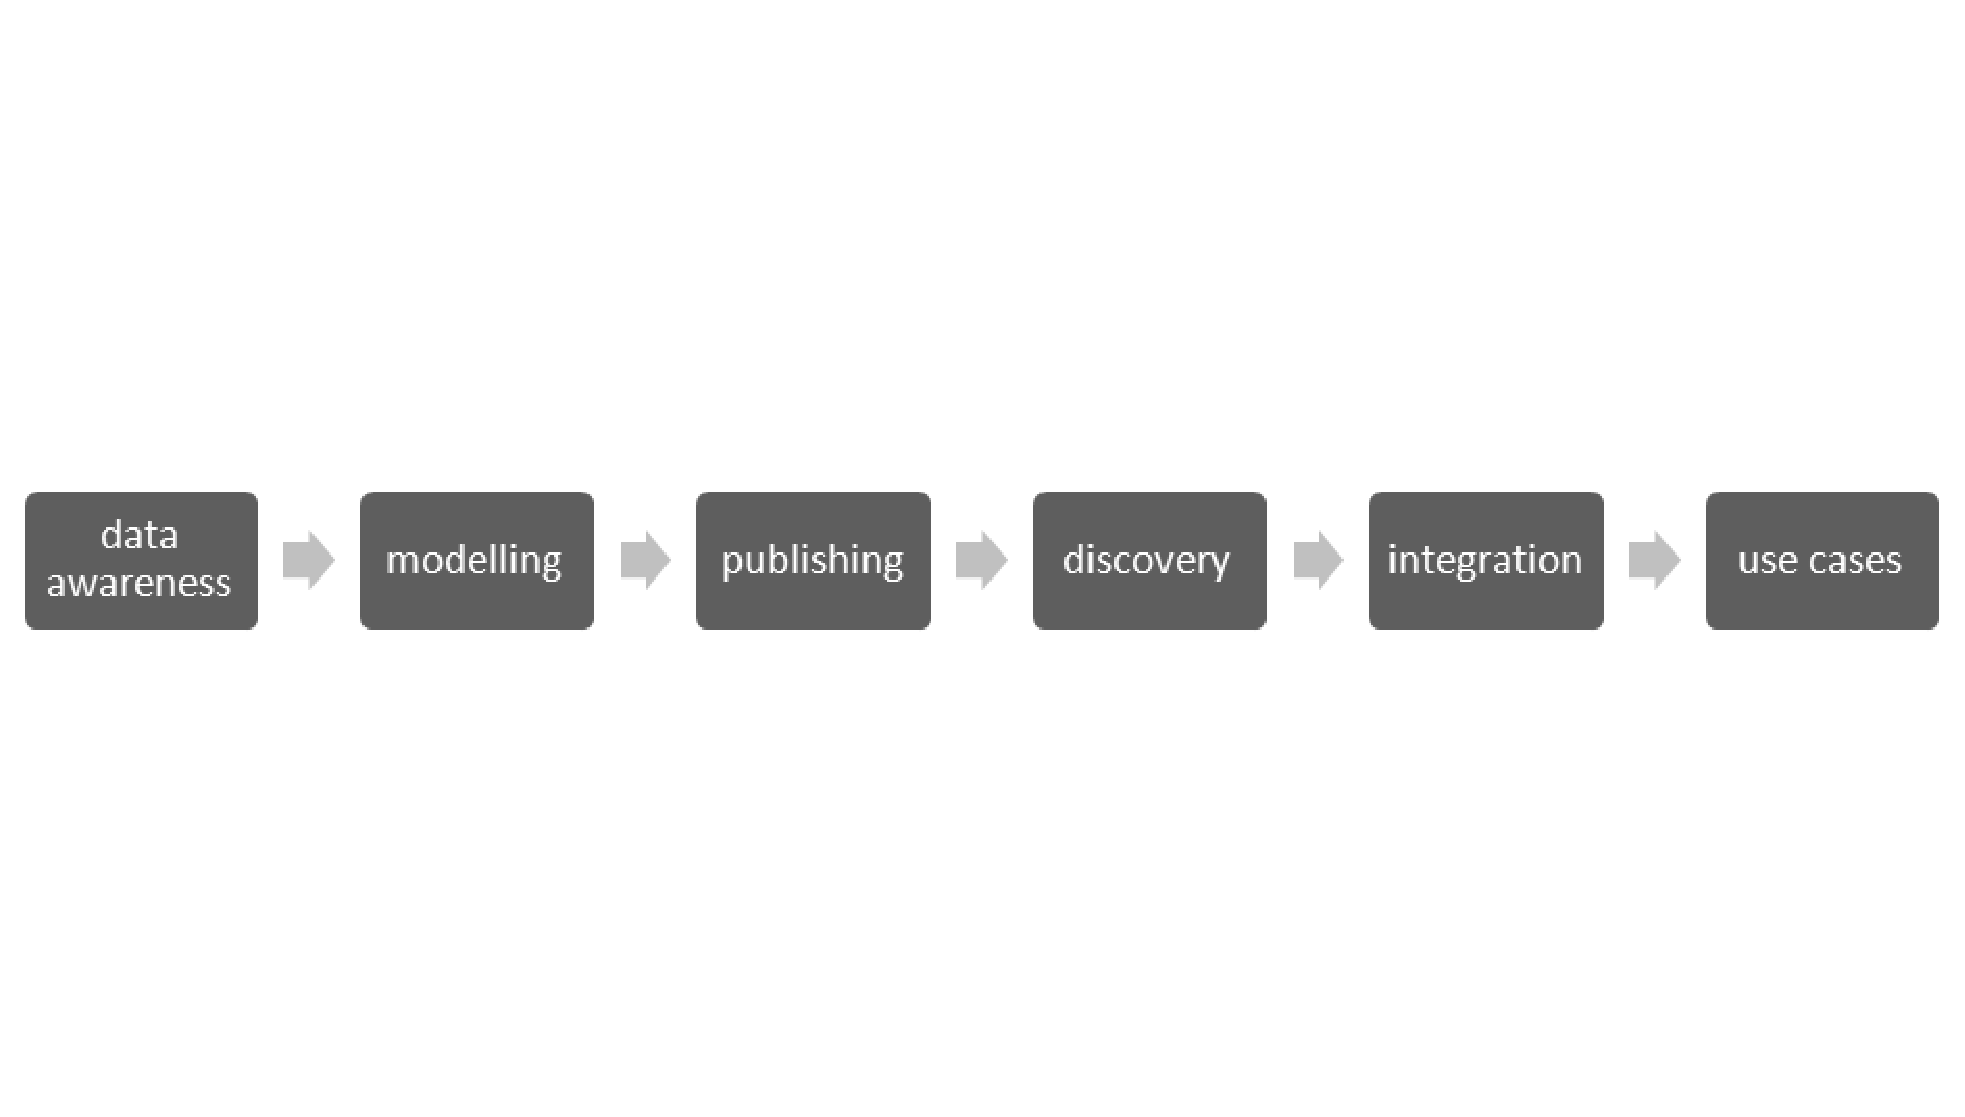
\includegraphics[width=14cm]{images/phd/Hausenblas}
\caption{\textit{Linked Data Lifecycle by M. Hausenblas}.}
\label{fig:hausenblas}
\end{figure}


 \item Boris Villazón-Terrazas, ver Figura~\ref{fig:boris}

\begin{figure}[!htb]
\centering
	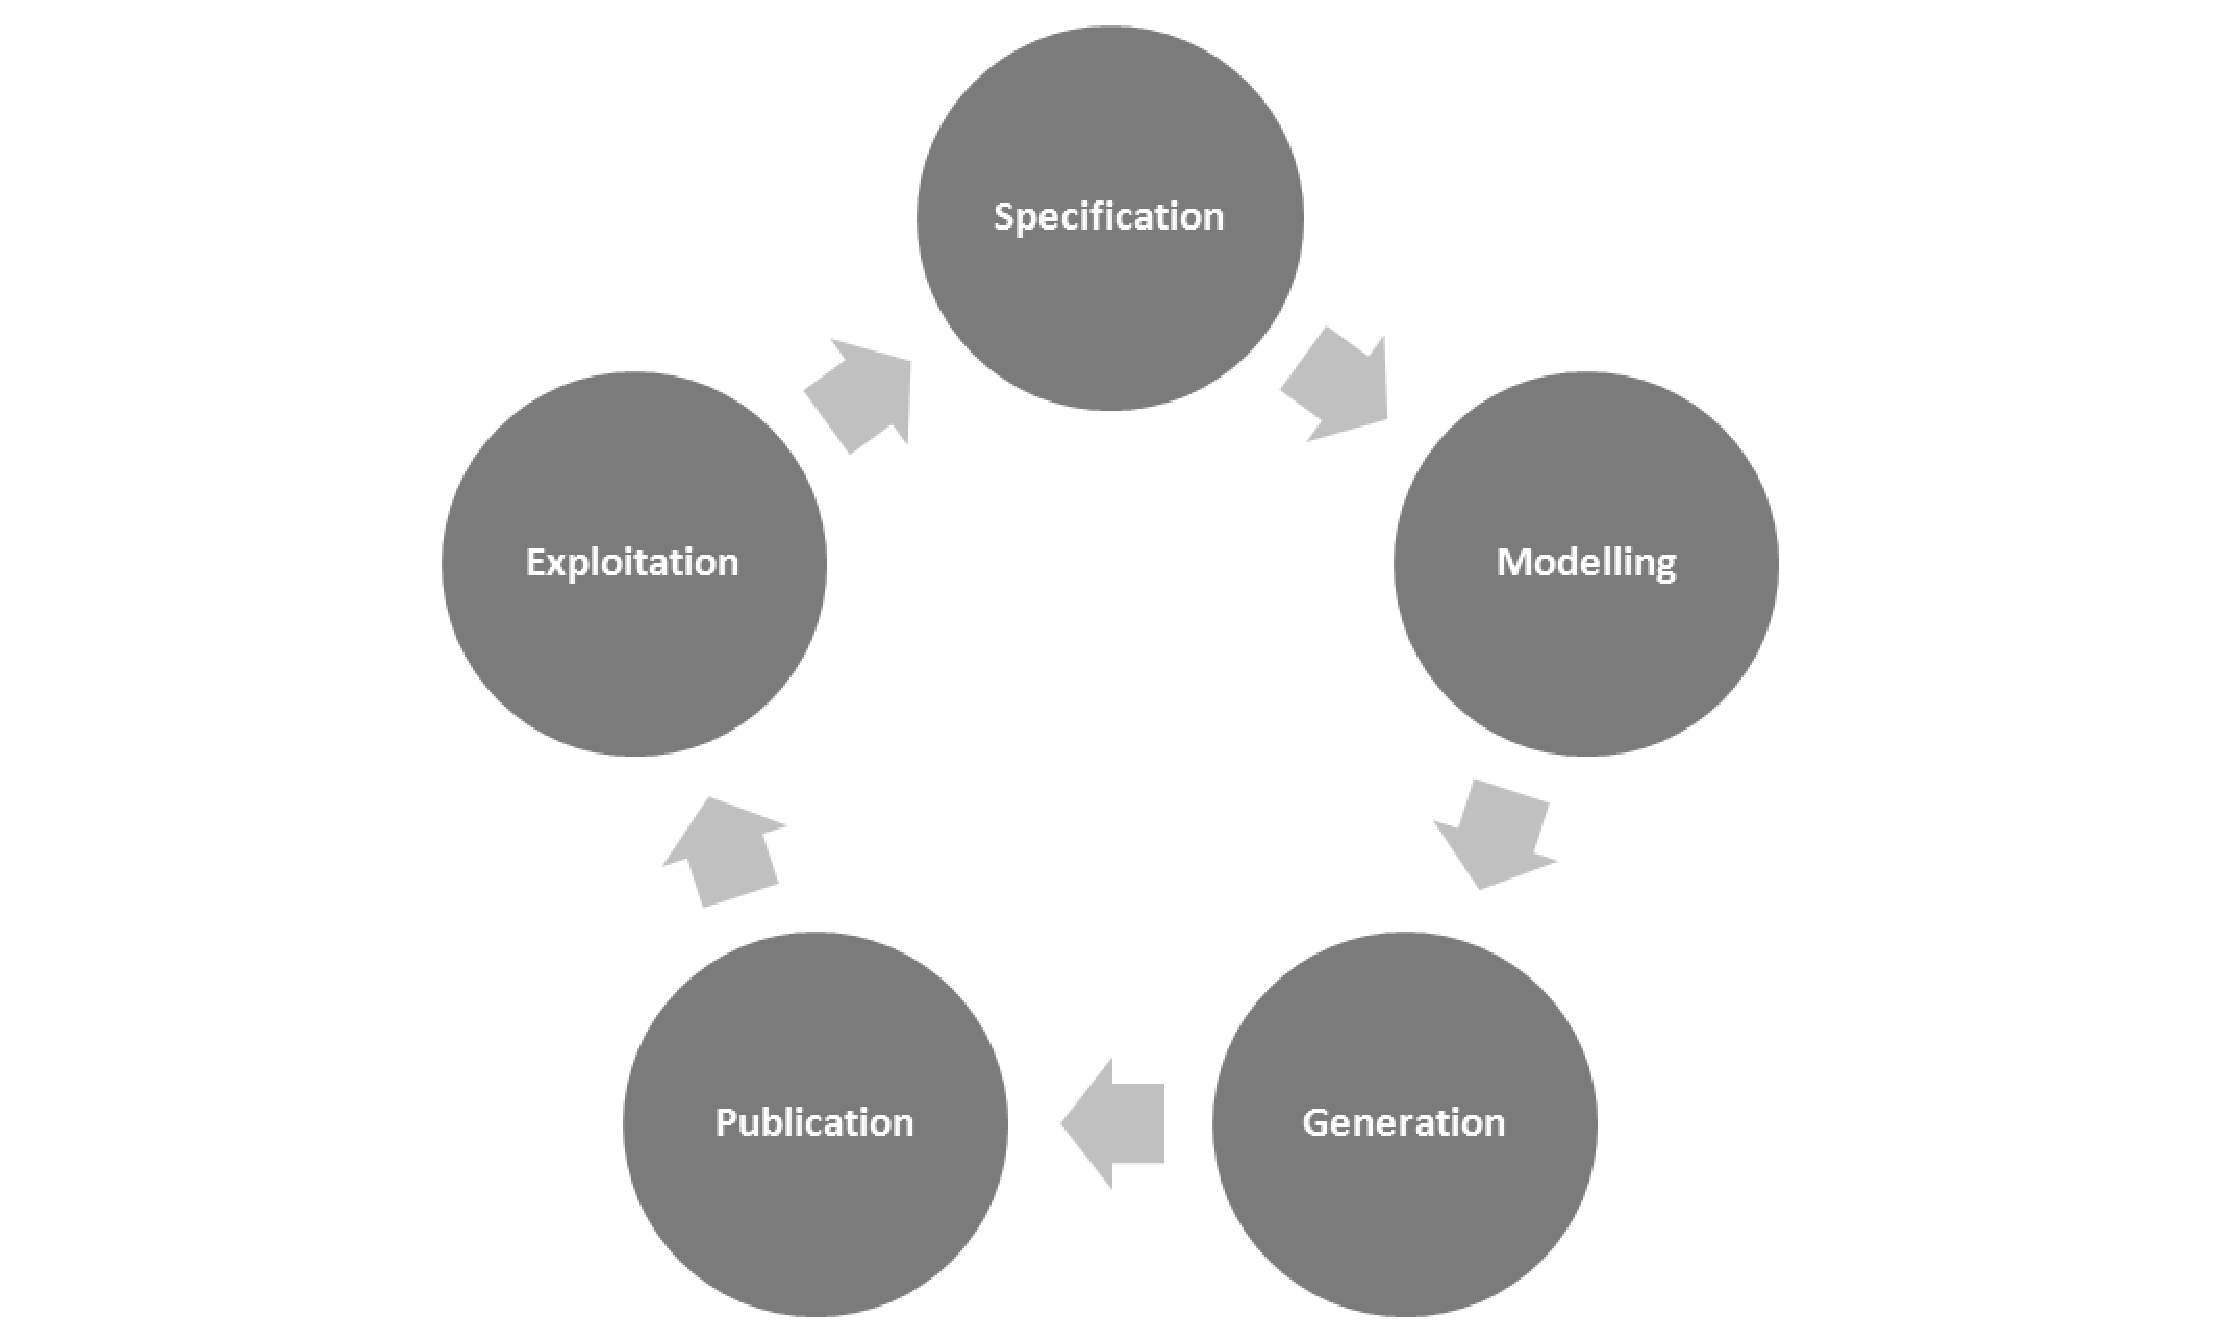
\includegraphics[width=14cm]{images/phd/Villazon-terrazas}
\caption{\textit{Linked Data Lifecycle by B. Villazón-Terrazas}.}
\label{fig:boris}
\end{figure}


 \item \textit{The DataLift Vision}, ver Figura~\ref{fig:datalift} 

\begin{figure}[!htb]
\centering
	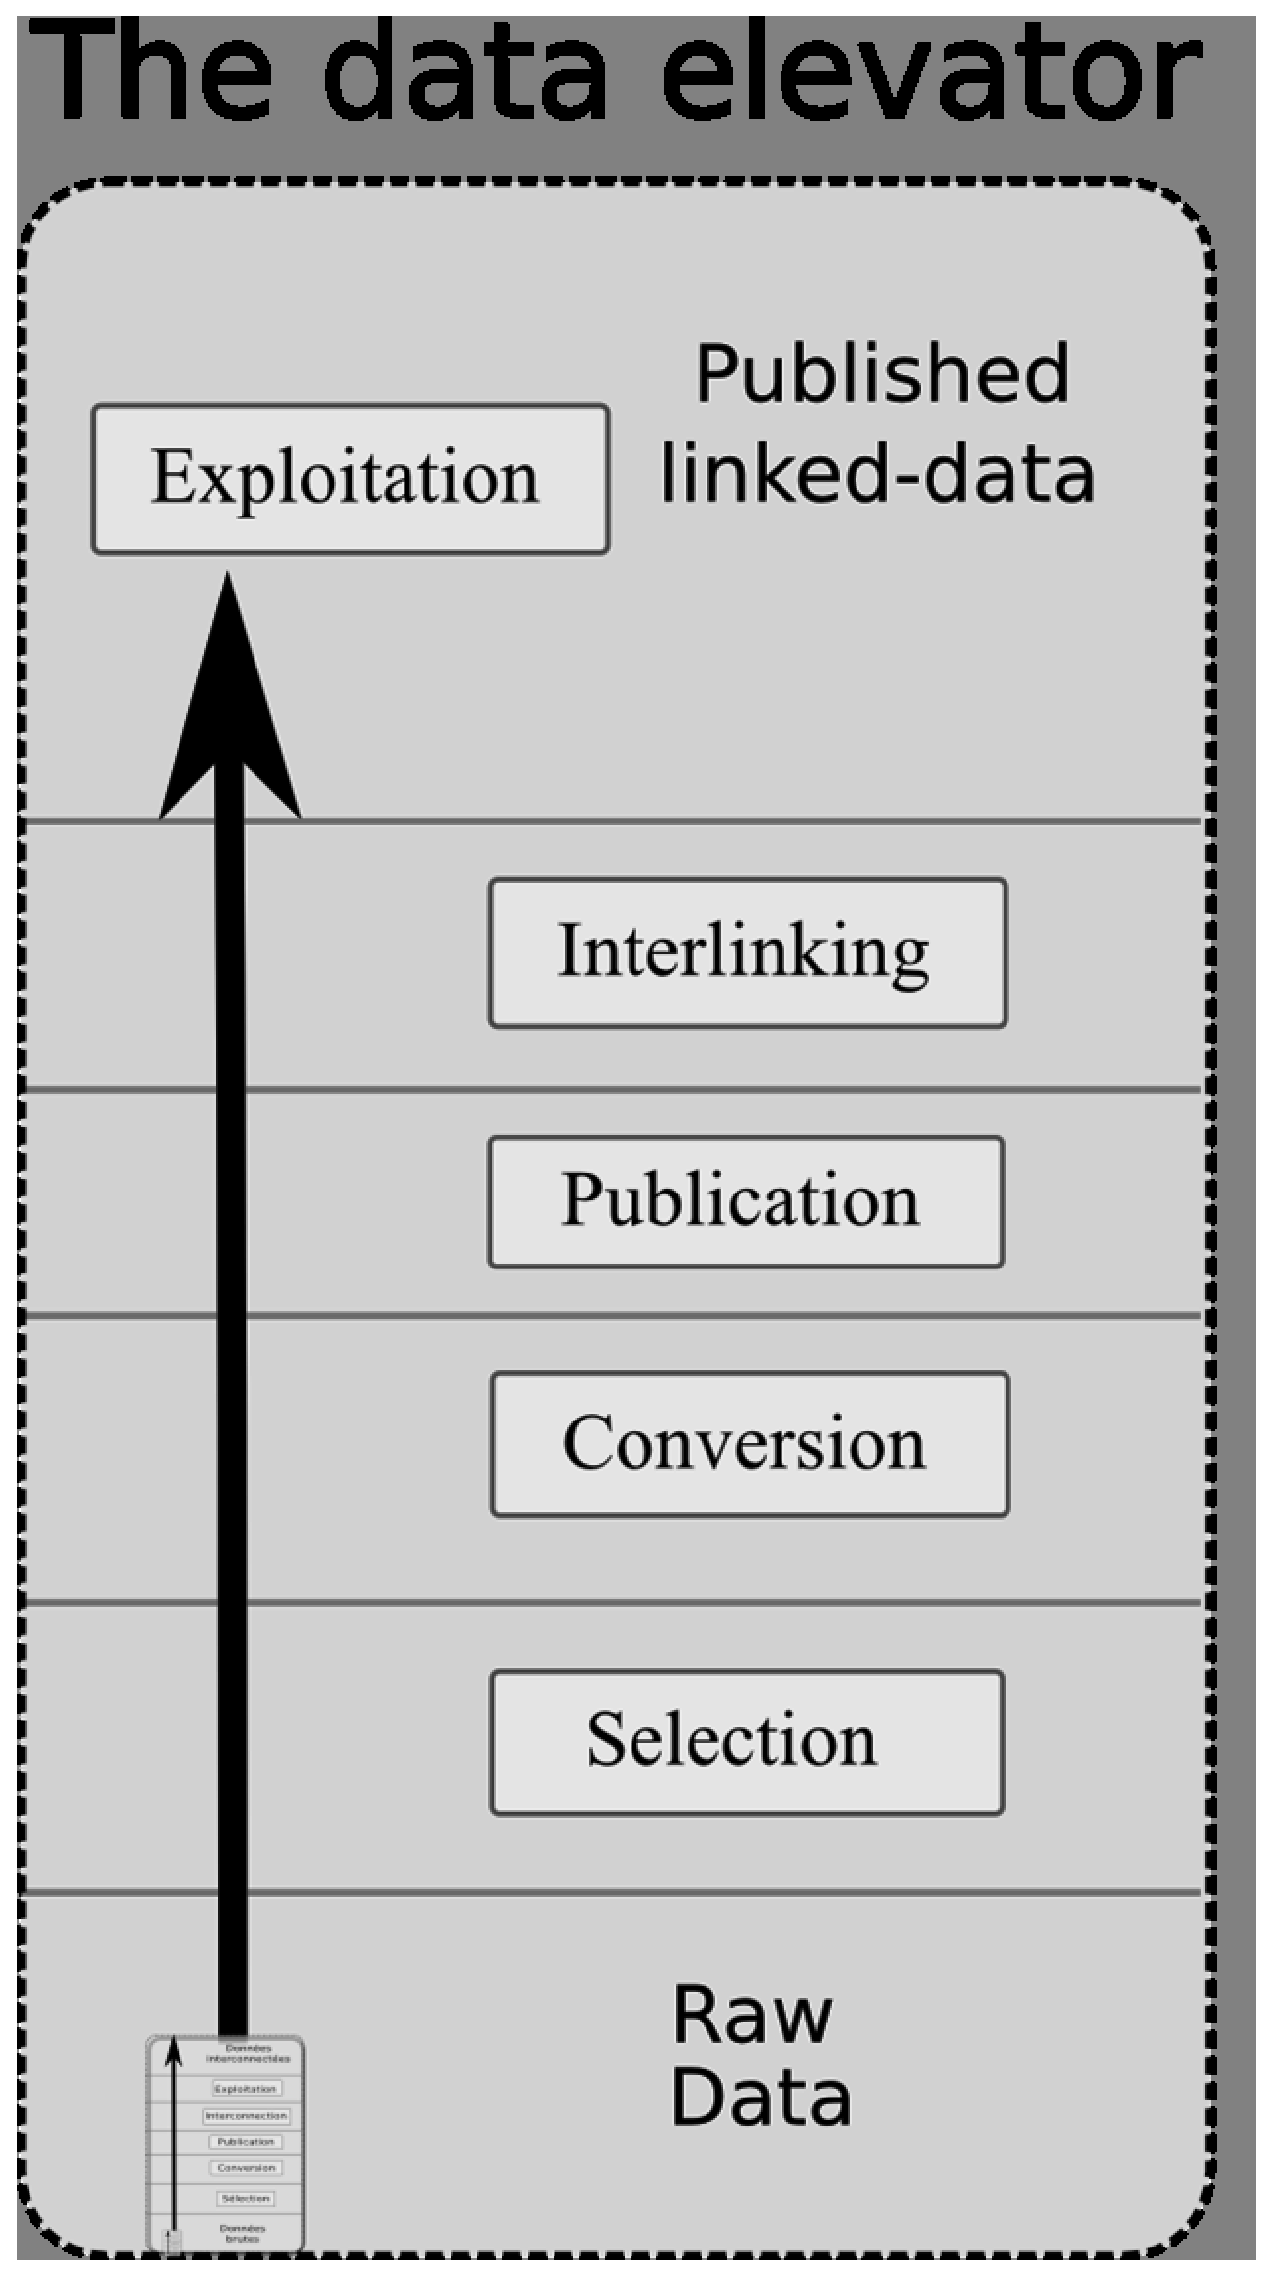
\includegraphics[width=6cm]{images/phd/Data_elevator}
\caption{\textit{DataLift Vision}.}
\label{fig:datalift}
\end{figure}
 \end{itemize}


En todos ellos se recogen en grandes procesos los pasos a seguir para desplegar el modelo de \linkeddata en una organización. Aunque
existan cambios en la denominación, en el nivel de abstracción o en el orden de algunos procesos, el objetivo coincide en todos ellos. No obstante, estos modelos han surgido, probablemente,
de la experiencia propia de los autores y aún estando en su etapa de desarrollo suponen un avance para afrontar la implantación
de \linkeddata como un proceso de ingeniería cuantificable.

\subsubsection{\textit{Publishing Open Government Data} del W3C}
Se trata de un borrador de trabajo~\cite{publishing-ogd} (\textit{W3C Working Draft 8 September 2009}) del grupo del \gls{W3C} \textit{\gls{eGovernment} Interest Group} en el cual
se hace una descripción somera sobre cómo publicar datos gubernamentales en la web. Reseñan fundamentalmente una serie de pasos 
para publicar datos sin grandes restricciones y de forma ágil, basándose en 3 pasos,
 ver Tabla~\ref{table:publish-ogd}, de carácter general pero que pueden servir especialmente a perfiles
no técnicos presentes en las instituciones públicas.

\begin{longtable}[c]{|l|p{7cm}|p{8cm}|} 
\hline
  \textbf{ID} & \textbf{Paso} & \textbf{Descripción} \\\hline
\endhead
  1 &  \textit{Step 1} & \textit{The quickest and easiest way to make data available on the Internet is to publish the data in its raw form.}\\ \hline
  2 &  \textit{Step 2} & \textit{Create an online catalog of the raw data (complete with documentation) so people can discover what has been posted.} \\ \hline
  3 &  \textit{Step 3} &   \textit{Make the data both human- and machine-readable.} \\ \hline
\hline
\caption{\textit{Straightforward Steps to Publish Government Data.}}\label{table:publish-ogd}\\    
\end{longtable}

De la misma forma, en el propio documento se exponen otros factores a tener en el momento
de publicación de los de datos y que van en la línea de la iniciativa de \linkeddata. Simplemente se trata
de una guía básica prácticamente de carácter divulgativo.

\subsubsection{\textit{LOD2 Stack}}\label{lod2-project}
Dentro del proyecto europeo LOD2~\cite{lod2-project} con nº de contrato: 257943, una duración desde septiembre de 2010
hasta agosto de 2014 y una financiación de más de $7$ millones euros se está desarrollando
una serie de documentos y tecnología asociada a la iniciativa de \lod con el objetivo de proveer
buenas prácticas y herramientas que den soporte a toda la cadena de producción, publicación y consumo
de datos enlazados en distintos dominios. Uno de los últimos resultados que han conseguido y que
se encuentra en continua evolución es la denominada \textit{LOD2 Stack}~\cite{lod2-stack} que contiene una
serie de herramientas para cada una de las etapas necesarias en la apertura de datos como \linkeddata.
Según la arquitectura de alto nivel, ver Figura~\ref{fig:lod-arch}, se identifican los siguientes componentes.

\begin{description}
 \item [\textit{OntoWiki}~\cite{tramp-s-2010-ekaw-demo}.] \textit{OntoWiki is a tool providing support for agile, distributed knowledge engineering scenarios}. 
 \item [\textit{PoolParty}~\cite{poolparty}.] \textit{PoolParty is a thesaurus management system and a SKOS editor for the Semantic Web including text mining and linked data capabilities.}
 \item [\textit{Sig.ma}~\cite{citeulike:8529753}.] \textit{Sig.ma is a tool to explore and leverage the Web of Data.}
 \item [\textit{Comprehensive Knowledge Archive Network (CKAN)~\cite{ckan}}.] \textit{CKAN is a registry or catalogue system for datasets or other ''knowledge'' resources.}
 \item [\textit{D2R Server}~\cite{Bizer_Cyganiak_2006}.] \textit{D2R Server is a tool for publishing relational databases on the Semantic Web. }
 \item [\textit{DBpedia Extraction}~\cite{Bizer:2009:D-C:1640541.1640848}.] \textit{DBpedia is a community effort to extract structured information from Wikipedia and to make this information available on the Web.}
 \item [\textit{DL-Learner}~\cite{lehmann2009}.] \textit{DL-Learner is a tool for supervised Machine Learning in OWL and Description Logics.}
 \item [\textit{MonetDB}~\cite{Boncz06monetdb/xquery:a}.] \textit{MonetDB is an open-source high-performance database system that allows to store relational, XML and RDF data}.
 \item [\textit{SemMF}.] \textit{SemMF is a flexible framework for calculating semantic similarity between objects that are represented as arbitrary RDF graphs.}
 \item [\textit{Silk Framework}~\cite{www2009227}.] \textit{The Silk Linking Framework supports data publishers in setting explicit RDF links between data items within different data sources.}
 \item [\textit{Sindice}~\cite{TummarelloDO07}.] \textit{Sindice is a state of the art infrastructure to process, consolidate and query the Web of Data. }
 \item [\textit{Sparallax}~\cite{Sparallax}.] \textit{Sparallax is a faceted browsing interface for SPARQL endpoints, based on Freebase Parallax.}
 \item [\textit{Triplify}~\cite{Triplify}.] \textit{Triplify provides a building block for the ``semantification'' of Web applications.}
 \item [\textit{OpenLink Virtuoso}~\cite{Virtuoso}.] \textit{Virtuoso is a knowledge store and virtualization platform that transparently integrates Data, Services, and Business Processes across the enterprise.}
 \item [\textit{WIQA}~\cite{wiqa}.] \textit{The Web Information Quality Assessment Framework is a set of software components that empowers information consumers to employ a wide range of different information quality assessment policies to filter information from the Web.} 
\end{description}

\begin{figure}[!htb]
\centering
	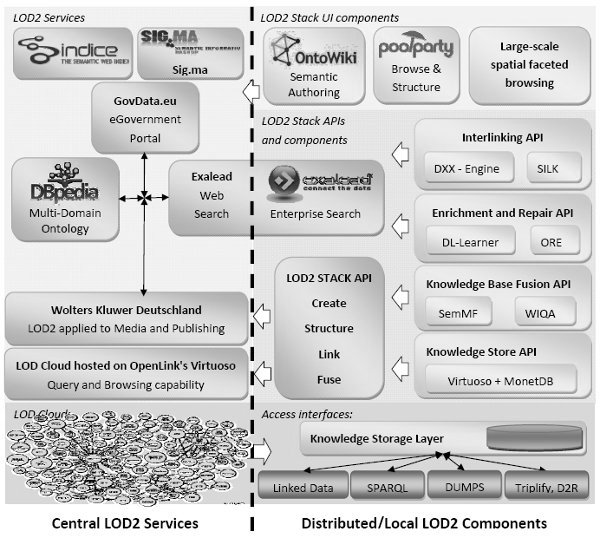
\includegraphics[width=10cm]{images/phd/lod2-high-level-architecture}
\caption{\textit{LOD2 high-level Architecturel} (extraída del portal del proyecto LOD2).}
\label{fig:lod-arch}
\end{figure}


Como se puede observar este grupo de herramientas dan soporte a todo el ciclo de vida de los datos enlazados y proveen
una plataforma genérica en la cual cualquier persona o entidad pueda integrar un nuevo conjunto de datos, desde
recursos ya disponibles en \gls{RDF} hasta documentos de texto. La realización de este proyecto es de una suma transcendencia
para la comunidad, ya que en el despliegue de una infraestructura basada en datos enlazados se suele incurrir en las mismas
dudas y problemas, por lo que el disponer de una guía que parta desde un punto de vista teórico hasta su realización práctica, 
supone una gran avance respecto a las especificaciones teóricas, recetas y buenas prácticas que se han mencionado en las
secciones anteriores. 

Por otra parte, las herramientas desarrolladas se encuentran enclavadas dentro de un proceso o ciclo de vida de datos enlazados,
ver Figura~\ref{fig:lod-lifecycle}. Se trata de un modelo iterativo y realimentado, en el cual se van pasando por distintas fases
para cumplir con la producción, publicación y consumo de datos, utilizando las herramientas previamente comentadas y atacando
las principales barreras que se suelen encontrar, así como aplicando los principios de diseño de \linkeddata.

\begin{figure}[!htb]
\centering
	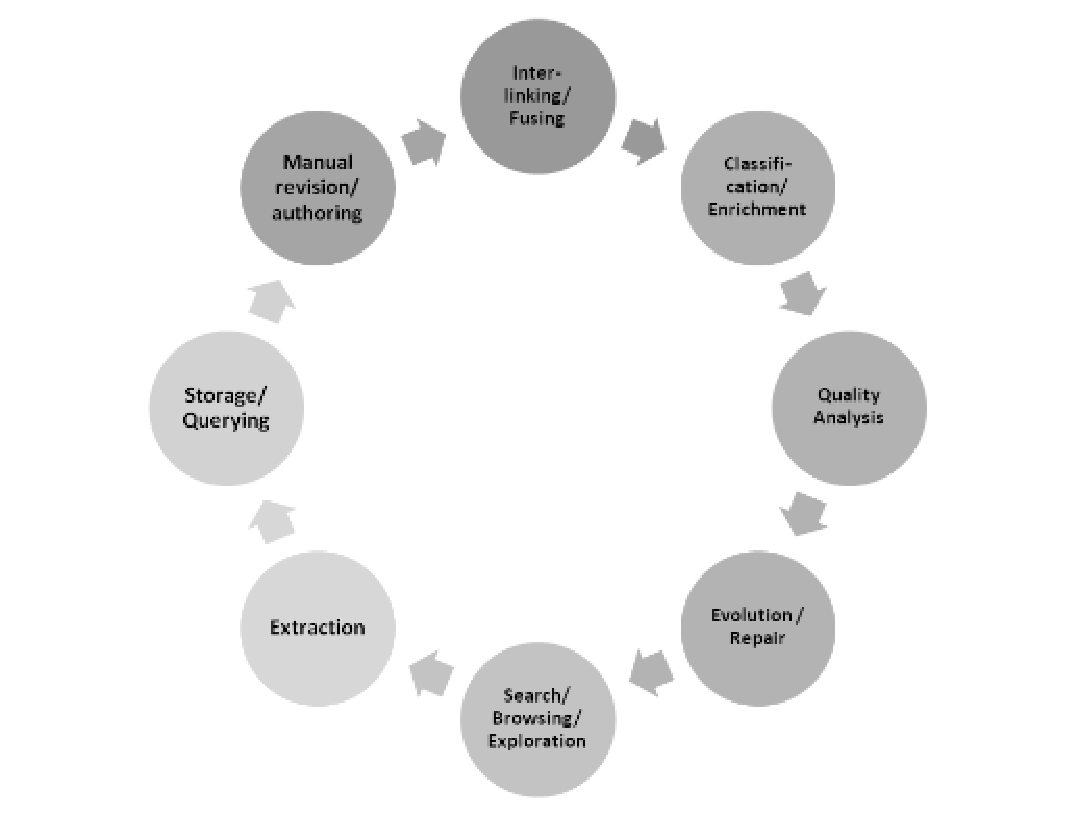
\includegraphics[width=12cm]{images/phd/lod-lifecycle-small}
\caption{\textit{Linked Data LifeCycle} (extraída de LOD2 Demo).}
\label{fig:lod-lifecycle}
\end{figure}

Para la aplicación de los principios de \linkeddata es realmente conveniente prestar atención al trabajo
desarrollado en este proyecto, no obstante, teniendo en cuenta que tan sólo se cuenta con un año de desarrollo
es complicado aplicar su enfoque de forma integral.

\subsubsection{\textit{Toward a Basic Profile for Linked Data} de IBM}
Dentro de la actividad de IBM en el campo de \linkeddata, se ha identificado
la necesidad de fijar una serie de reglas para aplicar esta iniciativa de forma
cuantificable. El objetivo de esta guía es llegar a introducir dentro de una herramienta
como \textit{Rationale} (también perteneciente a IBM) el modelo arquitectónico propuesto por los datos
enlazados, cumpliendo las directrices de la misma con la meta de obtener
la tecnología necesaria que sirva para integrar datos de forma ágil en las aplicaciones.

El término utilizado por IBM es ``Basic Profile Resources''~\cite{basic-profile-ibm} que se define como recursos \linkeddata accesibles mediante HTTP que siguen una serie de patrones
y convenciones comunes. En general, estos recursos dependen del dominio en el cual
estén definidos y tan sólo se delimitan como comunes unos pocos que se consideran
transversales a cualquier dominio. Estos recursos siguen una serie de reglas, ver Tabla~\ref{table:basic-ibm}, y reutilizan
vocabularios existentes con el objetivo de cumplir con la iniciativa de \linkeddata. 

\begin{longtable}[c]{|l|p{7cm}|p{8cm}|} 
\hline
  \textbf{ID} & \textbf{Rule} & \textbf{Descripción} \\\hline
\endhead
  1 &  \textit{Basic Profile Resources are \gls{HTTP} resources} & \textit{They can be created, modified, deleted and read using standard HTTP methods.}\\ \hline
  2 &  \textit{Basic Profile Resources use \gls{RDF} to define their states} & \textit{The state of a Basic Profile Resource (in the sense of state used in the REST architecture) is defined by a set of RDF triples.} \\ \hline
  3 &  \textit{You can request an RDF/XML representation of any Basic Profile Resource} &   \textit{The resource might have other representations.} \\ \hline
  4 &  \textit{Basic Profile clients use Optimistic Collision Detection during update} &   \textit{Because the update process involves getting a resource first, and then modifying it and later putting it back on the server, there is the possibility of a conflict (for example, another client might have updated the resource since the GET action). To mitigate this problem, Basic Profile implementations should use the HTTP If-Match header and HTTP ETags to detect collisions.} \\ \hline
  5 &  \textit{Basic Profile Resources use standard media types} &   \textit{ Basic Profile does not require and does not encourage the definition of any new media types.} \\ \hline
  6 &  \textit{Basic Profile Resources use standard vocabularies} &   \textit{Basic Profile Resources use common vocabularies (classes, properties, and so forth) for common concepts.} \\ \hline
  7 &  \textit{Basic Profile Resources set \texttt{rdf:type} explicitly.} &   \textit{A resource's membership in a class extent can be derived implicitly or indicated explicitly by a triple in the resource representation.} \\ \hline
  8 &  \textit{Basic Profile Resources use a restricted number of standard data types} &   \textit{RDF does not define data types to be used for property values, so Basic Profile lists a set of standard datatypes to be used in Basic Profile.} \\ \hline
  9 &  \textit{Basic Profile clients expect to encounter unknown properties and content} &   \textit{Basic Profile provides mechanisms for clients to discover lists of expected properties for resources for particular purposes.} \\ \hline
  10 &  \textit{Basic Profile clients do not assume the type of a resource at the end of a link} &   \textit{Many specifications and most traditional applications have a "closed model," by which we mean that any reference from a resource in the specification or application necessarily identifies a resource in the same specification.} \\ \hline
  11 &  \textit{Basic Profile servers implement simple validations for Create and Update} &   \textit{Basic Profile servers should try to make it easy for programmatic clients to create and update resources.} \\ \hline
  12 &  \textit{Basic Profile Resources always use simple RDF predicates to represent links} &   \textit{Basic Profile makes it very simple to know how links will appear in representations and also makes it very simple to query them.} \\ \hline
\hline
\caption{\textit{Basic Profile Resources.}}\label{table:basic-ibm}\\    
\end{longtable}

Repasando esta lista de reglas se puede observar como algunas afectan a los principios $2º$ y $3º$ de \linkeddata sin
modificar su significado pero especificando de forma más concreta el funcionamiento esperado. La importancia
de este reciente artículo reside en varios puntos: es realizado por IBM, es coherente con las reglas de \linkeddata y
ofrece un carácter práctico desde el punto de vista de la ingeniería para implementar, o en este caso, incluir
la arquitectura y modelo de trabajo de datos enlazados en una plataforma existente como es \textit{Rationale}.


\subsubsection{Metodología y Proceso de Adopción de \linkeddata en la Biblioteca del Congreso de Chile}
En este trabajo se propone una metodología~\cite{DBLP:conf/i-semantics/Cifuentes-SilvaSG11,methodologyCaepia2011} y proceso de adopción de la iniciativa de \linkeddata en el contexto
de las Administraciones Públicas y concretamente en la Biblioteca del Congreso de Chile para la publicación
de la legislación actual e histórica. En general, se trata en realidad de la especificación de una infraestructura
para dar soporte a los datos enlazados y un proceso de generación con diferentes etapas, que parten de un
caso particular motivador pero que se podrían aplicar a un contexto genérico. En la Figura~\ref{fig:bcn-infraestructura} se
pueden observar los distintos componentes que se proponen y que encajan con la infraestructura propuesta en 
el proyecto LOD2, ver Sección~\ref{lod2-project}. Una de las diferencias reside en las herramientas seleccionadas
para llevar a cabo los distintos procesos de producción, publicación y consumo de datos enlazados y por otra parte la
adición de servicios de consumo de datos especialmente dirigidos a los usuarios de la Administración, como es la visualización
de las normas.

\begin{figure}[!htb]
\centering
	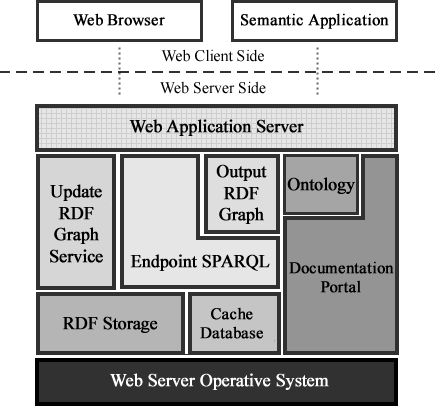
\includegraphics[width=10cm]{images/phd/infrastructure}
\caption{Infraestructra \linkeddata propuesta en la Biblioteca del Congreso de Chile.}
\label{fig:bcn-infraestructura}
\end{figure}

También, hay que destacar el proceso de adopción definido en este enfoque, ver Figura~\ref{fig:bcn-proceso}, en el cual
quedan recogidos los pasos para promocionar las bases de datos legislativas utilizando datos enlazados. Este proceso
es similar al propuesto por el \gls{W3C}, ver Sección~\ref{linked-data-cookbook}, y ciclo de vida definido en el proyecto LOD2, ver Figura~\ref{fig:lod-lifecycle}, 
difiere en el nombrado de los procesos y las herramientas a utilizar en cada una de las fases.

\begin{figure}[!htb]
\centering
	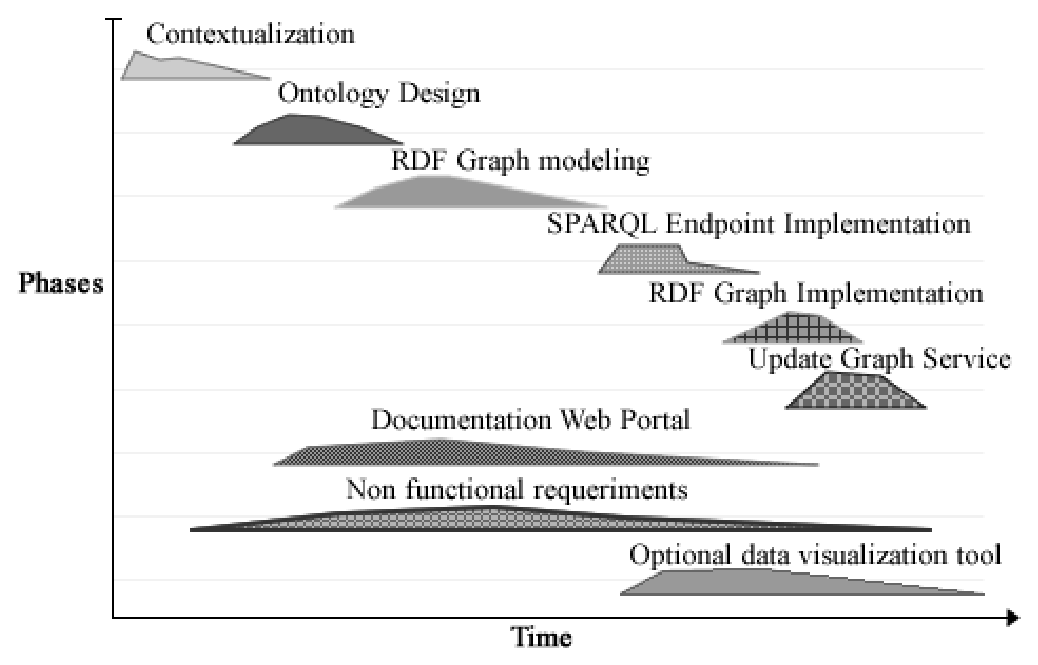
\includegraphics[width=10cm]{images/phd/process}
\caption{Proceso de implantación de \linkeddata en la Biblioteca del Congreso de Chile.}
\label{fig:bcn-proceso}
\end{figure}


\subsubsection{\textit{Talis Platform}}
En este caso la plataforma Talis~\cite{talis} es un servicio o producto que sirve para la creación de una
infraestructura de \linkeddata en la nube. Ha tenido un gran éxito ya que sus creadores son grandes
impulsores de la iniciativa (por ejemplo son los autores de ``Linked Data Patterns'') y han trabajado
en casos de enorme repercusión, como la apertura de datos públicos del Gobierno del Reino Unido. Ofrecen 
 una ``suite'' de herramientas y servicios para cumplir las directrices de \linkeddata, teniendo en cuenta 
la mayor parte de la casuística presente en la producción, publicación y consumo de datos enlazados. En resumen, se provee una plataforma
que cubre toda la cadena de valor de los datos enlazados y cumple todas las directrices necesarias.

Entre las características más llamativas que ofrecen dentro de esta plataforma se encuentran las
siguientes (extraídas de la propia página web de Talis):

\begin{itemize}
    \item \textit{A simple, consistent web API for storing, managing and retrieving both structured and unstructured data.}
    \item \textit{Flexible, schema-free metadata that allows applications to be easily evolved.}
    \item \textit{A range of data access and query options enabling easy integration into both new and existing applications.}
    \item \textit{Access control options to support hosting of both public and private data.}
    \item \textit{A data hosting solution that is founded on open internet standards and web architectural best practices.}
    \item \textit{Software as a Service, enabling rapid development with zero deployment costs.}
    \item \textit{Low, even free, utility based pricing for services and hosting allowing costs to grow with usage.}
    \item \textit{A highly available and scalable infrastructure to ensure that the repository grows in line with your applications needs.}
\end{itemize}

Evidentemente este tipo de soluciones son de extraordinario interés para las Administraciones Públicas, ya que consiguen
un producto llave en mano con todas las capacidades necesarias para disponer de una infraestructura de datos
enlazados de última generación. Es interesante destacar esta plataforma por dos motivos principales: sus creadores
son relevantes desde un punto de vista científico y han realizado una gran transferencia tecnológica desde
el campo de la investigación al industrial.

En la misma línea de la plataforma Talis podemos encontrar otras empresas que ofrecen productos y herramientas
de alto valor como son Virtuoso de OpenLink o ToqQuadrant. Todos ellos son miembros activos en la comunidad
de \linkeddata y están presentes en los principales grupos de trabajo de esta iniciativa en el \gls{W3C}.
 
\subsubsection{\textit{Linked Open Data: The Essentials}}\label{linked-data-spec}
Este libro~\cite{Bauer2012} realizado en colaboración entre \gls{REEEP} (\textit{Renewable Energy and Energy Efficiency Partnership}) y la compañía \textit{Semantic Web}
es un manual que da respuesta a algunas de las preguntas comunes que surgen en el despliegue de una infraestructura de datos enlazados
en el seno de una organización. En general, se trata de una recopilación de las buenas prácticas que se han revisado
en los anteriores apartados y que focaliza en los beneficios de la publicación de datos enlazados para las
organizaciones. La parte más destacada de este libro, ver Figura~\ref{fig:lod-essentials}, se centra en la descripción de las tareas
a realizar y de los posibles servicios haciendo hincapié en las tareas de publicación y consumo de datos enlazados.

\begin{figure}[!htb]
\centering
	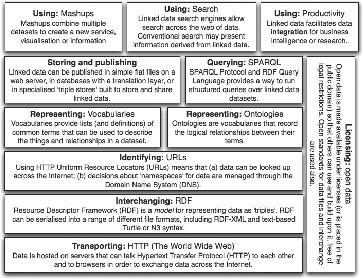
\includegraphics[width=10cm]{images/phd/lod-essentials}
\caption{\textit{Elementos of the Linked Open Data Puzzle}.}
\label{fig:lod-essentials}
\end{figure}


\subsubsection{Documentación específica}\label{linked-data-spec}
Desde distintas organizaciones tales como Administraciones Públicas y Universidades,
así como personalidades relevantes en esta materia se ha promovido la realización de proyectos, guías y artículos que tratan diversos aspectos
relacionados con la iniciativa de \linkeddata. Todos ellos tratan de aportar nuevos enfoques, herramientas y documentación
a los distintos procesos implicados en el despliegue de esta iniciativa, entre los que podemos destacar:

\begin{itemize}
 \item ``\textit{A Proposal for Governmental Data URIs}'' realizado por Gregory Todd Williams, Tim Lebo y Alvaro Graves.  % http://iw.rpi.edu/wiki/A_Proposal_for_Governmental_Data_URIs
 \item ``\textit{Designing \gls{URI} Sets for the UK Public Sector}''~\cite{uris-uk} realizado por ``The Cabinet Office'' del Reino Unido. 
 \item ``\textit{Federal Information Security Management Act (FISMA)}'' proyecto realizado por  el ``National Institute of Standards and Technology'' de Estados Unidos.
 \item La documentación disponible en la Biblioteca del Congreso de Estados Unidos.
 \item Los artículos de Jeni Tennison sobre distintos aspectos relativos al diseño de URIs, etc.
 \item El \textit{framework} SERIMI~\cite{Serimi} de reconciliación de entidades.
 \item Los documentos y software elaborados por la empresa Epimorphics.
 \item Las guías de datos abiertos y enlazados de las distintas Administraciones Públicas, tanto a nivel estatal 
España, Reino Unido, Francia, Alemania, etc., como a nivel regional, Asturias, País Vasco o Cataluña o incluso local como
en el Ayuntamiento de Zaragoza.
\end{itemize}

En general se trata de documentos o herramientas que nacen de la necesidad y experiencia en la resolución de ciertos
 problemas relacionados con la apertura de datos y su enlazado, que se reproducen en cada escenario en el cual se
aplica esta iniciativa. Todo este trabajo y esfuerzo supone un gran valor para la comunidad de desarrolladores
y de personas implicadas en aplicar estos principios.

\subsection{Escenarios y Casos de Uso de Éxito}
La irrupción de la corriente de \linkeddata ha conllevado la realización práctica y real de una parte de la denostada Web
Semántica. Muchas son las instituciones, administraciones públicas,
empresas privadas, universidades, hospitales, que bajo esta corriente están
liberando sus datos en el entorno web siguiendo las directrices  marcadas por
Tim Berners-Lee. El principal objetivo consiste en la apertura de datos, para que
una vez publicados sirvan como fuente para la creación de aplicaciones agregando
distintos recursos (\textit{mashups}), facilitando la transparencia de comportamiento en
ciertos organismos, suministrando servicios de valor añadido basados en el contexto
del usuario o simplemente desde un punto de vista de tendencia, para obtener
presencia en la nueva \wod. 

No obstante, este nuevo enfoque conlleva varios desafíos a nivel científico que están siendo
abordados actualmente, tales como el procesamiento de grandes cantidades de
datos de forma eficiente, gestión-formalización-explotación del conocimiento
subyacente mediante reglas, razonamiento distribuido, \textit{stream-reasoning}, \textit{real
time linked data}, \textit{complex event processing}, reconciliación de entidades,
visualización etc., los casos de uso de aplicación de estas investigaciones representan un abanico muy amplio: recomendación de recursos
(películas, libros, etc.), análisis de sentimientos y opiniones, domótica,
\textit{smart-cities}, computación ubicua, \textit{green computing}, sistemas de soporte a la
decisión en campos como \textit{e-Health}, etc.

Hasta el momento esta iniciativa ha estado muy ligada al mundo técnico, es decir, tanto la publicación como el 
consumo de los datos estaba muy orientado a un perfil fundamentalmente técnico. No obstante, al igual que con la web que hoy conocemos, 
la \wod todavía no trascendido al gran público, es por ello que surgen varios desafíos~\cite{DBLP:journals/semweb/DadzieR11} para conseguir que el despegue definitivo 
de esta corriente:

\begin{enumerate}
 \item Necesidad de una capa de presentación. Si una persona buscara cierto recurso 
 que tiene definido según unas necesidades, la expresión de esta consulta implicaría características de 
sistemas de \textit{Information Retrieval} o tareas de análisis de sentimientos. Más en concreto: a) descubrimiento de qué fuentes pueden tener 
disponible esa información; b) validación y cooperación entre las distintas fuentes de datos disponibles; c) consulta a 
las fuentes de datos seleccionadas y d) análisis, presentación y manejo de las vistas de los resultados. En este sentido, la tendencia actual 
reside en ``ocultar'' la existencia de varios datasets detrás de los sistemas de búsqueda, así como la consulta y manejo de los 
resultados, de tal manera que el usuario no es consciente de las oportunidades de explotación de datos de las que podría disponer. 
Es necesario aclarar que el conocimiento de la tecnología no debe ser la clave para la explotación de la misma por el usuario 
final, pero si que es necesario proveer los métodos y herramientas adecuadas para que el usuario obtenga el máximo partido de 
la información subyacente. De esta manera si la tendencia de \linkeddata supone una revolución respecto a la actual web de documentos, se 
deberían proveer nuevos mecanismos de acceso a la información y no restringirse a los tradicionales modelos de interacción con el 
usuario (por ejemplo un formulario de búsqueda). 
\item Combinación efectiva de los distintos \datasets. Teniendo en cuenta que existe un catálogo de datos y 
  vocabularios en constante crecimiento, es necesario proveer los mecanismos necesarios (alineación, \textit{mapeo} y fusión) para que 
la combinación de los mismos sea eficiente en el sentido de que la identificación de recursos similares, el 
encaje mediante propiedades o la mezcla de recursos sea intuitiva, tanto desde un punto de vista técnico como del usuario final. 
Las técnicas que permiten llevar a cabo este desafío no son deterministas y en muchos casos se basan en algoritmos que chequean 
la estructura de los recursos o bien realizan comparaciones basadas en procesamiento del lenguaje natural entre las descripciones de los recursos.
\end{enumerate}

En el contexto de \linkeddata surgen dos principales vías de actuación sobre los datos: publicación y consumo, concretamente en el campo de consumo de 
datos surgen varios interrogantes como:
\begin{itemize}
\item Gestión de datos a nivel web.
\item Procesamiento de consultas federadas~\cite{sparqlOpt}.
\item Búsqueda.
\item Descubrimiento de \datasets y recursos: URIs, datos adicionales o datasets relevantes para una consulta.
\item \textit{Datasets} evolutivos: cómo afectan los cambios en los datasets a las consultas, monitorización.
\item Razonamiento e inferencia de conocimiento en la \wod.
\item Calidad de los datos: evaluación de la calidad de la información, confianza y \textit{provenance}.
\item Interfaz de Usuario para la interacción con la \wod: interacción y usabilidad, visualización, interfaces basadas en lenguaje natural.
\end{itemize}


Por otra parte, en las Administraciones Públicas se está trabajando exhaustivamente en el campo de la reutilización de datos, en la actualidad 
se pueden señalar algunos ejemplos:
\begin{itemize}
\item Gestión de bibliotecas digitales, la Biblioteca del Congreso de Chile o del Congreso de Estados Unidos.
\item Gestión de flotas. Aplicación del Ayuntamiento de Gijón para el control de la línea urbana de autobuses .
\item Sistemas de búsqueda y recomendación basadas en perfiles usuario enlazados.
\item Sistemas de e-Health. Para el soporte a la decisión en el diagnóstico.
\item Sistemas de Información Geográfica. GIS+Linked Data.
\item Gestión y publicación de información financiera.
\item Otros múltiples campos de actuación: Turismo, Tráfico, Educación, Domótica, \textit{Semantic Sensors}, etc.
\end{itemize}

En último término todas las iniciativas basadas en \linkeddata convergen al objetivo principal de la misma:
\begin{Frame}
\textit{Linked Data is about using the Web to connect related data that wasn't previously linked, or using the Web to lower the barriers 
to linking data currently linked using other methods.} 
\end{Frame}


Teniendo en cuenta el valor añadido de la visualización de datos para Linked Data,
 se pueden establecer una serie de requisitos~\cite{journals/semweb/DadzieR11} a cumplir, que actualmente están parcialmente cubiertos 
por algunas herramientas, no obstante, se puede establecer una guía de características necesarias para el manejo de datos enlazados y su 
visualización, siendo uno de los grandes elementos de investigación actual.
\begin{itemize}
 \item Requisitos de alto nivel: a) capacidad para generar vistas agregadas de los datos; b) soporte para la creación de filtros y c) soporte para 
la visualización detallada de los recursos.
\item  Requisitos de consumo de datos: a) manejo de datos multidimensionales; b) manejo de datos jerárquicos;
c) generación de estructuras de representación: grafos, árboles, etc.; d) identificación de las relaciones significativas en los datos;
e) extracción de datos y nuevas relaciones y f) contextualización de usuario y multidispositivo.
\item Requisitos directamente relacionados con \linkeddata: a) navegación entre los distintos datasets; b) exploración de los datos 
para obtener consciencia de la estructura y de las relaciones; c) exploración que permita análisis con el objetivo de identificar incoherencias, etc.;
d) consulta transversal a través de los distintos datasets mediante un lenguaje formal y e) capacidad para extraer partes de los datos para su posterior reutilización.
\item Requisitos relacionados con la navegación semántica: a) navegación facetada y contextualizada del usuario; b) exploración del conocimiento, inferencia, etc.;
c) consulta avanzada con filtros de lenguaje natural; d) análisis detallado y explicación de las inferencias y e) presentación de resultados de análisis.
\end{itemize}





\section{\label{capitulo:eproc-sm}Tendencias actuales en Semántica} 
El creciente uso de Internet durante los últimos años ha puesto de manifiesto un
nuevo entorno de ejecución para las aplicaciones, utilizando como nueva
plataforma la web, el gran sistema distribuido. Nuevas tecnologías y paradigmas
están emergiendo para dar soporte al desarrollo y despliegue de aplicaciones y
servicios, así como para la publicación de datos e información. Los modelos de
desarrollo están cambiando a un estilo más colaborativo en el cual las empresas
ofrecen su software como servicios (\textit{Software as a Service}-\gls{SaaS}) materializado a
través del paradigma de \textit{cloud computing}~\cite{Armbrust09abovethe}, implementado con tecnología de
servicios con el objetivo de que terceros puedan utilizar estos servicios para
la construcción de aplicaciones agregadas con valor añadido. 

En este sentido, tal como se ha señalado, iniciativas como la Web Semántica, que a través de modelos y
formatos de datos de conocimiento compartido unificados, intentan elevar el
significado de los elementos y recursos que están disponibles en la web, con el
objetivo de mejorar la integración e interoperabilidad entre aplicaciones, están 
impulsando la implantación de este enfoque. Dentro de la iniciativa de Web
Semántica hay que destacar dos esfuerzos: 
\begin{enumerate}
 \item La iniciativa \linkeddata que tal y como se ha descrito propone la publicación de datos
enlazados siguiendo el modelo \gls{RDF} para facilitar la creación de una web de
datos en la que éstos se puedan mostrar, intercambiar y conectar a través de
URIs. La tendencia actual de publicación de datos enlazados está marcando una
evolución en la interoperabilidad de aplicaciones, con el consiguiente efecto que
conlleva para las relaciones \gls{B2B}, \gls{B2C} o \gls{A2A}. Entre los casos de éxito
podrían destacarse: administración electrónica (iniciativa de \textit{Open Government
Data}, contratación pública de bienes y servicios (\eproc), oferta formacional , contextualización de aplicaciones, \textit{mashups},
etc. 

\item El desarrollo de lenguajes y formalismos lógicos para representar el conocimiento sobre un universo de discurso, permitiendo la inferencia de nuevos
datos a partir de los datos ya publicados. En este contexto se ha impulsado nuevamente el uso de las técnicas de razonamiento y de sistemas basados en conocimiento, como 
las ontologías y los sistemas basados en reglas (Ontobroker, XSB, etc.) o de producción (Drools , JRules , etc.). 
La aplicación de estos sistemas está ampliamente asentada en la resolución de diversos problemas
(diagnóstico, planificación, reglas de negocio, etc.) pero siempre utilizando un enfoque para la representación del conocimiento y de los datos, en muchos casos
específico y no estandarizado. Por tanto, debe tenerse en cuenta la flexibilidad, tanto para la integración como para la interoperabilidad de las aplicaciones. Una arquitectura orientada a
servicios sobre la plataforma web, utilizando los protocolos actuales y que se beneficie de las iniciativas relativas a la Web Semántica puede dar respuesta a
este punto clave. La implantación de un sistema basado en conocimiento, concretamente de
sistemas basados en reglas y de razonamiento, que hagan uso de una infraestructura estandarizada y cooperativa redunda en gran beneficio para la
resolución de problemas basados en conocimiento declarativo y compartido, mejorando tanto la independencia tecnológica de las aplicaciones como la experiencia de usuario.
\end{enumerate}


Al amparo de la visión de la Web Semántica, el \gls{W3C} ha promovido la creación de varias recomendaciones que intentan ofrecer soluciones 
para las diferentes capas de la arquitectura. En concreto, RDF es el lenguaje de representación básico que 
permite representar tripletas de la forma sujeto-predicado-objeto. Dichas tripletas 
forman un grafo dirigido que puede integrarse automáticamente con otros grafos obtenidos de otros servidores. 
Otra de las tecnologías propuestas por el W3C es RDFS, que permite la definición de clases, propiedades e individuos y 
ofrece unos mecanismos básicos de inferencia mediante reglas. RDFS facilita la creación e integración de vocabularios 
pero carece de expresividad suficiente para describir relaciones avanzadas como complementos de conjuntos o cardinalidades. Las limitaciones 
expresivas de RDFS propiciaron la definición de \gls{OWL}, un lenguaje de definición de ontologías basado en lógica descriptiva. 
La versión 2 de OWL llegó a status de recomendación del W3C en octubre del año 2009. Una de las principales mejoras de esta versión, estaba 
encaminada a la resolución del compromiso entre la expresividad y la complejidad de los razonamientos, mediante la definición de perfiles o 
fragmentos computacionales. Los tres perfiles de OWL2: EL, QL y RL, son sublenguajes del mismo que permiten alcanzar una complejidad 
polinómica para tareas de razonamiento estándar limitando la expresividad. La combinación de OWL con lenguajes basados en 
reglas que incluyen la negación, como los \textit{dl-programs}~\cite{DBLP:conf/rr/Motik08} han sido desarrollados en las redes de excelencia 
\textit{REWERSE} y \textit{Knowledge web} y definen la interoperabilidad entre las reglas y las ontologías. 

El problema del intercambio de reglas entre los distintos sistemas de razonamiento e inferencia también ha sido abordado recientemente, 
así encontramos la recomendación del W3C RIF de 22 de junio del año 2010. 
\gls{RIF} es, de nuevo, una familia de lenguajes (\textit{Core},\textit{Production Rule Dialect, BLD Basic Logic Dialect, Datatypes and Built-Ins, Framework for Logic Dialects}, etc.) 
con diferente expresividad, cuyo objetivo es convertirse en \textit{lingua franca} para el intercambio de conocimiento basado en reglas en la web. 
El formato utilizado por RIF es \gls{XML} y su combinación con ontologías permite que las reglas y el modelo de datos sobre los que se van a aplicar 
las reglas se pueden intercambiar entre distintos actores. Para interpretar RIF es necesario realizar una traducción desde este vocabulario al motor de inferencia
deseado. En el ámbito de intercambio de reglas hay que resaltar el antecesor de RIF, RuleML que es una iniciativa internacional sin ánimo de lucro, que cubre
los aspectos del intercambio y la interoperabilidad de reglas. Esta iniciativa mantiene una estrecha relación con los grupos de OASIS en reglas, así como con
ISO Common Logic (estándar en el año 2007). RuleML, como grupo, también contribuye en \gls{OMG} a \gls{SBVR}, específicamente en el apartado de \textit{Production Rule Representation} (PRR) cuya última
versión data de diciembre del año 2009.

Para la consulta de datos \gls{RDF} se ha desarrollado \gls{SPARQL}, un lenguaje de consulta y un
protocolo de acceso que permiten definir un terminal (o \textit{endpoint}) en el que se publican conjuntos de datos (o \textit{datasets}) RDF y 
que están disponibles como servicios en la web. Actualmente se está trabajando en vocabularios para
definir datasets y poder enlazarlos entre sí de forma sencilla. Con el uso de
SPARQL han aparecido propuestas para la definición de reglas de producción con
este lenguaje (extensión \textit{SPARQL with Updates-\gls{SPARUL})} de modo que se ejecuten
directamente sobre una base de datos en RDF, como puede ser SPARQL-Rules~\cite{citeulike:1294570},
también existen enfoques para la consulta de ontologías OWL con SPARQL~\cite{Sirin07sparql-dl:sparql} y
en la especificación que se elabora actualmente, SPARQL 1.1, se
dispone de un vocabulario para definir los servicios disponibles. Finalmente y
con el objetivo de personalizar la vista de las aplicaciones por el usuario y su
contextualización se ha aplicado el uso de reglas en formato \gls{JSON}~\cite{conf/ki/GiurcaP08}. 


La evolución de los formalismos para definir ontologías lleva emparejado el
desarrollo de razonadores que puedan llevar a cabo las inferencias necesarias.
Desde el pionero KL-ONE hasta este momento, se han implementado múltiples
razonadores basados en lógica descriptiva siguiendo diferentes técnicas. En la
actualidad, se pueden destacar Fact++~\cite{Tsarkov2006}, Pellet~\cite{Sirin_Parsia_Grau_Kalyanpur_Katz_2007} y RacerPro~\cite{Rajeev2001Racer}
que se basan en la técnica conocida como \textit{semantic tableaux}. A pesar de las altas
complejidades, en el caso peor los algoritmos de razonamiento utilizados en estos sistemas son capaces de resolver muchas tareas prácticas gracias al uso de
diversas optimizaciones. Para resolver dichas limitaciones, especialmente, al
tratar con grandes cantidades de datos, se han buscado técnicas alternativas
como el algoritmo de resolución utilizado en KAON2~\cite{journals/ercim/Motik08}, el sistema
\textit{hipertableau} empleado en HermiT~\cite{msh09hypertableau}, las técnicas de eliminación de tipos~\cite{DBLP:conf/aaai/RudolphKH08}
 o las recientes técnicas basadas en eliminación de consecuentes~\cite{DBLP:conf/ijcai/SimancikKH11}.

La utilización de reglas se ha propuesto como una alternativa para la
implementación de razonadores. En este caso, las definiciones de la ontología
son compiladas a un conjunto de reglas, que se aplica al conjunto de datos para obtener las inferencias correspondientes. La principal
ventaja de estos razonadores es que se basan en técnicas ya conocidas en el
ámbito de la programación lógica con diversas implementaciones disponibles, constituye sin embargo una
desventaja, que generalmente es necesario utilizar subconjuntos de \gls{OWL}, como el
conocido OWL Horst~\cite{Horst2005}. Uno de los mayores retos de la Web Semántica es la búsqueda de técnicas que
mejoren la escalabilidad de los razonadores, en esta línea, han surgido
trabajos que proponen la utilización de tecnologías distribuidas para afrontar
dicha complejidad. Por ejemplo, en~\cite{SomaPrasanna2008}
se propone la implementación de un sistema de inferencia paralelizable sobre OWL
Horst, mediante un particionado de las reglas. Con el objetivo de mejorar la
escalabilidad, en~\cite{springerlink:10.1007/978-3-642-04930-9_43} se propone un algoritmo para realizar inferencias sobre
RDFS que se aplica a un \textit{benchmark} de $10.000$ tripletas, proponiendo como trabajo futuro la posible aplicación de MapReduce~\cite{citeulike:430834,DBLP:conf/semweb/UrbaniKOH09}. En~\cite{UrbaniMaassenBal2010} se describe una implementación basada en el algoritmo MapReduce
logrando realizar el cierre parcial de $864$ millones de tripletas en RDFS, en una
hora utilizando 32 procesadores. Recientemente, los mismos autores
desarrollaron el sistema WebPIE~\cite{Urbani2010WebPIE}, el cual ha sido capaz de
realizar inferencias sobre $1$ billón y medio de tripletas, en $6,1$ horas utilizando
$32$ nodos, mediante reglas de OWL Horst. El sistema SAOR se ha implementado para
dar soporte al buscador semántico SWSE, incorporando un razonador sobre OWL
Horst~\cite{HoganHarthPolleres2009}, dicho sistema ha diseñado un nuevo algoritmo
distribuido, mejorando la escalabilidad de la implementación~\cite{DBLP:conf/semweb/HoganPPD10}. Finalmente, también se está 
trabajando~\cite{HausenblasCloudLOD} en la conjunción de \linkeddata y \textit{cloud computing} para el procesamiento de grandes cantidades de datos.


\section{\label{capitulo:eproc-sm}\textit{e-Procurement} y Semántica} 
La construcción de un modelo semántico sobre un dominio de negocio concreto
consiste en el desarrollo de un sistema de conocimiento que describa las
entidades y propiedades, así como las relaciones lógicas que existen entre
las mismas. Un aspecto, muchas veces minusvalorado, es que en estos modelos de
dominio es necesario describir también los procesos, las restricciones y en
general, los aspectos dinámicos del dominio. Este tipo de modelos formalizados
mediante un lenguaje lógico, como ya se ha descrito, se denominan ``ontologías''. La selección de la lógica apropiada para la modelización de 
la base de conocimiento no es una cuestión sencilla y se deberán contemplar diferentes
factores tales como grado de computabilidad, decidibilidad, soporte razonadores, etc. Existen
diferentes vocabularios y lenguajes que permiten modelar un cierto dominio, algunos
de los cuales ya se han repasado (\gls{RDF}, RDFS, \gls{OWL} y \gls{WSML}) en la Sección~\ref{sect:arch-ws}, no obstante, existen otros estrechamente
ligados a entornos de negocio, que a continuación se presentan.


\begin{description}
\item[\gls{RIF} (\textit{Rule Interchange Format})~\cite{rif-core}.] RIF constituye una familia de lenguajes con diferente expresividad, 
cuyo objetivo es convertirse en \textit{lingua franca} para el intercambio de
conocimiento basado en reglas en la Web. Define la compatibilidad con
documentos RDF y OWL, además está especialmente diseñado para integrarse con
sistemas de inferencia basados tanto en reglas de producción, como de
Programación Lógica. La ventaja de RIF respecto de OWL es una mayor expresividad, 
que permite expresar conocimiento causal y procedimental. 


\item [\gls{SCOR} Model (\textit{Supply-Chain Operations Reference-Model}).] Es un modelo conceptual de
referencia para la especificación y formalización de los procesos de negocio
asociados a las cadenas de suministro. Este modelo define los procesos de
planificación, fabricación, entrega, evolución e inventarios de productos en una
cadena logística.

\item [\gls{SBVR} (\textit{Semantics of Business Vocabulary and Business Rules}).] Es un estándar
(ISO 704/1087) desarrollado por el \textit{Object Management Group} (\gls{OMG}). Define un
metamodelo para el desarrollo de modelos semánticos de vocabularios y reglas de
negocio. La idea es que a partir del lenguaje natural se puedan expresar
vocabularios y reglas de negocio en un dominio concreto. La construcción de un
modelo de negocio mediante el SBVR recoge el vocabulario de conceptos del
dominio y la definición de lógica formal asociada.

\item [Clasificaciones de productos de comercio electrónico~\cite{Leukel-ecatalog2005,Leukel-standard,Leukel-automating}.] Para
facilitar el intercambio automático de información y la anotación de los diferentes productos
y documentos que forman parte del comercio electrónico, distintos sectores de
actividad económica han desarrollado sus propias terminologías o
vocabularios~\cite{Norbert-class} controlados, para armonizar mediante códigos unívocos la identificación de
los objetos de negocio. Ejemplos de estos vocabularios son: el estándar eCl@ss o
la clasificación \gls{UNSPSC} entre otros, ver Sección~\ref{sect:pscs}.


\item [\gls{ebXML} (\textit{Electronic Business using eXtensible Markup Language}).] Es un lenguaje
\gls{XML} elaborado por \gls{OASIS} y UN/CEFACT, también consta de una infraestructura que permite la comunicación entre entidades
participantes en transacciones de negocio electrónico, favoreciendo la interoperabilidad y la seguridad de una forma homogénea entre las distintas partes.
La propuesta original cubría cinco capas: \textit{Business processes}; \textit{Collaboration protocol agreements};
\textit{Core data components}; \textit{Messaging} y \textit{Registries and repositories}.

eBXML ha sido aprobado por \gls{ISO} en un conjunto de especificaciones, ISO 15000:  ISO 15000-1: ebXML \textit{Collaborative Partner Profile Agreement};
ISO 15000-2: ebXML \textit{Messaging Service Specification}; ISO 15000-3: \textit{ebXML Registry Information Model}; ISO 15000-4: ebXML \textit{Registry Services Specification};
y ISO 15000-5: ebXML \textit{Core Components Technical Specification}, Version 2.01.

\item [\gls{XBRL} (\textit{extensible Business Reporting Language}).] 
Es una norma elaborada en el año 1998 por Charles Hoffman, contable y auditor, para
simplificar la automatización del intercambio de información financiera mediante
el uso del lenguaje XML. La familia de lenguajes XBRL se ha realizado para
satisfacer las exigencias principalmente de información financiera y
empresarial, permite aplicar etiquetas identificativas multilenguaje con
significado, por ejemplo indicando si es un valor monetario, también es posible
mostrar la relación que guardan los elementos entre sí, así se podría saber cómo se
calculan. Una característica muy importante es la capacidad de extensión, de
esta forma es capaz de adaptarse para casos particulares de empresas. 

\end{description}

\subsection{Actividades de aplicación de Semántica en \textit{e-Procurement}}
Desde la creación del movimiento de la Web Semántica, en concreto de la realización
práctica mediante \linkeddata, se han aplicado los principios de estas iniciativas a múltiples
dominios como ya se ha reseñado en las secciones anteriores. Evidentemente en un sector como 
la Administración Pública, caracterizado por su amplitud, casuística y carácter estratégico para todos los ciudadanos
es por lo que la semántica y sobre todo las corrientes de \opendata y \linkeddata han penetrado con mucha fuerza en los últimos años. 
En un principio los esfuerzos como en otros dominios, se centraban en el modelado de la administración
como organización y de sus procesos, con el objetivo de mejorar la interoperabilidad e integración
entre las aplicaciones y facilitar los trámites burocráticos. En muchos casos se han desplegado
soluciones flexibles basadas en la reutilización de información, procesos y conocimiento a través
de grandes bases de datos compartidas, servicios web y sistemas basados en reglas, no obstante la inmersión
de la semántica propiamente dicha se centraba en la realización de modelos para formalizar
cuestiones relativas a documentación y a procesos administrativos. Por ello,
la irrupción de \opendata y \linkeddata ha reorientado el esfuerzo de las Administraciones Públicas
para aprovechar la semántica en su beneficio. 

Por otra parte, también han surgido iniciativas~\cite{DBLP:journals/tcci/Alor-HernandezAJPRMBG10} relacionadas con \eproc, pero desde un punto de vista
de las cadenas de suministro, en las cuales se modelan de forma completa un entorno de proveedores y suministros mediante la coordinación
de los recursos software, hardware y humanos propios de un entorno de este tipo, como son \gls{ERP}s, robots o las propias personas. 

\subsubsection{Ontología de Contratos Públicos del proyecto LOTED}
El diseño de la ontología en el proyecto LOTED~\cite{loted-project}, es de suma importancia debido a su consideración 
como primer gran esfuerzo por aunar las iniciativas de \linkeddata y \opendata en el campo de la contratación 
pública electrónica. En este proyecto la propuesta principal consiste en la transformación directa 
de la información proveniente del \gls{RSS} de \gls{TED} a \gls{RDF} para su posterior indexado en un repositorio y acceso 
mediante un \textit{endpoint} de \gls{SPARQL}. Como sucede un muchos casos relacionados con la iniciativa 
de \linkeddata la ontología realizada, ver Figura~\ref{fig:public-contracts-ontology-loted}, está orientada a la representación de los datos en sí, estableciendo 
un modelo formal en el cual enclavar los recursos RDF generados, pero si bien este enfoque es válido, tan sólo 
representa una parte de la casuística presente en el dominio de la contratación pública electrónica. El intento 
realizado en TED se centra en el diseño de las entidades presentes en la información del RSS para así suministrar 
un modelo formal a los recursos RDF. Por todo ello, esta ontología sirve como una gran fuente de información 
para comprobar que tipo de entidades se recogen o publican en el RSS de TED, pero en un espectro más amplio 
se considera insuficiente para la representación de información teniendo en cuenta los modelos de datos 
disponibles en las plataformas de contratación o el propio de \gls{opXML} realizado en el proyecto ``10ders Information 
Services'', como ha quedado señalado en la Sección~\ref{data-model-eproc}. 

Por otra lado y desde el punto de vista del acceso a los datos, se ofrece la posibilidad de la realización 
de consultas en SPARQL seleccionando una serie de códigos y acotando los resultados por fechas, sin embargo este sistema 
parece desactualizado y no se han realizado cambios en los últimos dos años. 

\begin{figure}[h]
 \centering
    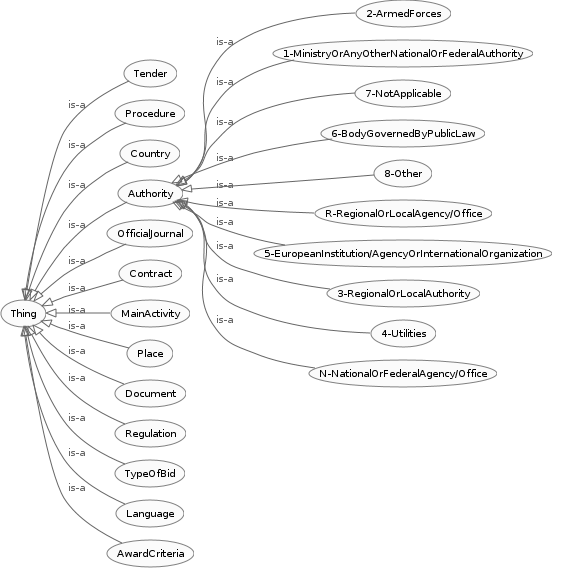
\includegraphics[width=14cm]{images/phd/loted-ontology}
  \caption{Ontología de Contratos Públicos del proyecto LOTED.}
 \label{fig:public-contracts-ontology-loted}
\end{figure}

\subsubsection{Ontología de Contratos Públicos de la República Checa}
Esta ontología está siendo desarrollada por el grupo \textit{Knowledge Engineering Group} 
de la \textit{Charles University} de Praga en la República Checa. Parte del esfuerzo está siendo
cubierto parcialmente dentro del proyecto europeo LOD2 en su paquete de trabajo \textit{WP9A – LOD2 for a Distributed Marketplace for Public Sector Contracts}, cuya descripción es la siguiente:

\begin{Frame}
\textit{The objective of this use case is to explore and demonstrate the application of linked data principles for procuring contracts in the public sector...}
\end{Frame}

Este trabajo enlaza perfectamente con el propósito de este documento, esto es cubrir el sector de los contratos
públicos con semántica y concretamente con la iniciativa \linkeddata. Es por ello que se ha establecido
contacto con los integrantes del grupo de investigación de esta Universidad para aprovechar y realimentar
esfuerzos, como fruto de esta colaboración han empezado a reutilizar los códigos CPV, resultado de este trabajo y del proyecto ``10ders Information Services''.

La ontología que se ha desarrollado en este grupo, ver Figura~\ref{fig:public-contracts-ontology}, tiene como intención recoger
la información y datos de los contratos públicos de forma estructurada, para que pueda ser consumida
automáticamente tanto por personas como por máquinas, desarrollándose también dentro del ámbito
de la iniciativa de \opendata de la República Checa. Desde un punto de vista del diseño reutiliza varios
vocabularios y ontologías ya disponibles, como \textit{Payments Ontology} del Reino Unido, lo que confiere a este modelo un carácter integrador y 
reutilizable. No obstante, abordar la descripción de toda la casuística del proceso de contratación pública electrónica parece
muy ambicioso y podría presentar problemas de interoperabilidad, integración y reutilización ya que 
puede estar muy orientada a la problemática de un entorno particular. Otro de los puntos importantes
que se deben abordar, y parcialmente recogidos en esta ontología y que deben servir de guía, están referidos a 
la adición de metainformación para \textit{provenance}, licencia, etc., que si bien en algunos
\datasets es importante, en la información de carácter público es fundamental y debe ser un requisito
para las propias entidades públicas.

\begin{figure}[h]
 \centering
    \includegraphics[width=14cm]{images/phd/public-contracts-ontology}
  \caption{\textit{Public Contracts Ontology from Czech Republic.}}
 \label{fig:public-contracts-ontology}
\end{figure}


\subsubsection{Clasificaciones Estándar de Productos}\label{semantica:pscs}
Las clasificaciones de productos, son instrumentos claves de estandarización~\cite{Leukel-standard} que nacen con el fin de
conseguir una clasificación común de productos y servicios. En general, son variadas~\cite{Leukel-ecatalog2005}
y obedecen a intereses particulares dependiendo del sector como e@Class o RossetaNET,
o bien de carácter global como \gls{UNSPSC} u otras destinadas a un dominio particular como el \gls{CPV} en la Administración Pública, ver Sección~\ref{sect:pscs}. Las diferencias
estriban en su alcance y cobertura sectorial, pero también en el grado de especificidad o nivel
de profundidad que existe para describir los productos o servicios.

Como señala Hepp\cite{HeppTrueComplexity,HeppEclass,HeppMethodology} todos estos
estándares reflejan una combinación de componentes variables, que pueden ser
utilizados para la construcción de una ontología derivada a partir de la clasificación.
Sin embargo, se puede identificar una estructura común subyacente a todas ellas y
que es fundamental señalar para proporcionar un modelo de datos semántico universal para este tipo de clasificaciones, consistente 
en que todas estas clasificaciones se ordenan jerárquicamente. 

\begin{description}
 \item [Categorías de productos.] Las clasificaciones se dividen en categorías o
clases de productos, agrupando los distintos elementos del catálogo.
\begin{itemize}
 \item Las categorías de la clasificación se organizan jerárquicamente.
 \item Cada elemento de la clasificación pertenece a una categoría de
productos.
 \item Cada elemento de la clasificación pertenece sólo una categoría de
productos, es decir, las categorías son disjuntas.
\end{itemize}

\item  [Estructura taxonómica.] Además de la división en niveles de jerarquía
de los elementos de la clasificación, su objetivo es organizar y agrupar los productos en
sectores verticales mediante algún tipo de criterio establecido por la comunidad
que desarrolla el estándar. 
 
\end{description}

Estas son características genéricas de las clasificaciones de productos. Sin
embargo, otras clasificaciones más sofisticadas incluyen un diccionario de propiedades
estándar que se puede utilizar para describir productos con más detalle.
Normalmente, estos diccionarios de propiedades también incluyen los tipos de
datos que pueden ser valor de las mismas, así como su referencia con respecto a estándares internacionales para establecer las unidades de medida, este es el caso
de la clasificación de productos de e@Class. En otras ocasiones, se construyen
clasificaciones multiling\"{u}es para la expresión de los descriptores de cada
elemento. 

La irrupción de la tecnología semántica y, sobre todo, la aparición de
lenguajes web para la representación de conocimiento y gestión de metadatos, ha
propiciado un creciente interés en el uso de las clasificaciones estándar de productos para mejorar tanto el
intercambio de información, como su capacidad para estructurar información. La construcción de ontologías de productos 
con alto nivel de detalle implican un coste que es muy difícil de asumir en muchos casos. 
Los autores~\cite{Yu:2009:CSI:1693684.1693743,FenselOmel2001,FenselDing2001} comparten la opinión de Corcho~\cite{CorchoECommerce} 
de que una ontología de productos sería muy útil para la organización conceptual del mercado, se entiende que estas ontologías tienen
más carácter privado, para la organización de la producción, los departamentos
de ventas y comerciales y, en general, para cualquier área de una empresa o
institución que deba tratar con la gestión de productos.

El desafío básico más importante que hay que afrontar cuando se deriva una
ontología de una clasificación de productos, se refiere a cómo interpretar la semántica original de la taxonomía.
No existe una definición formal de las relaciones taxonómicas que construyen
cada categoría de la clasificación y es tentador utilizar la propiedad de un
vocabulario de ontologías, como \textit{rdfs:subClassOf}, para intentar
representar estas relaciones semánticas, sin embargo, esta suposición es errónea. Como señala~\cite{HeppMethodology}, esta relación de jerarquía entre los elementos no se puede considerar
equivalente a una relación de subclase o de herencia. En primer
lugar, tomando el siguiente ejemplo: el elemento ``Partes y accesorios de
bicicleta'' del \gls{CPV} 2008 (34432000-4) tiene como antecesor a ``Bicicletas''
(34440000-0), donde la relación semántica entre los dos elementos no es
herencia, es decir, no se puede expresar que una \textbf{parte de una bicicleta}
sea una \textbf{bicicleta}. Para ser más precisos, debería modelarse como una relación de
composición o agregación. En este sentido, ocurre igual con la relación
taxonómica entre ``Tubos de resina Epoxi''(19522110-5) y ``Resina Epoxi''
(19522100-2), en el que es difícil justificar de nuevo una relación de herencia
clásica entre el primero y el segundo elemento del CPV, ya que en ningún caso
se puede considerar que el continente y el contenido de un objeto complejo tenga
el mismo estatus en una ontología de dominio, es decir, que un \textbf{tubo} no
es un tipo de \textbf{resina}.

Pero no sólo es complicado interpretar correctamente las relaciones semánticas
que codifica la taxonomía de una clasificación de productos, desde el punto de vista de las ontologías
como modelos de conocimiento de dominio, muchos elementos de una clasificación de productos son
difícilmente interpretables como conceptos de dominio, en este sentido, un elemento como ``Barras, varillas, perfiles y alambre de
estaño'' (27623100-9) del CPV 2003, que parece más una colección
artificial de productos que una clase estructural, en la que sus instancias
comparten algún tipo de propiedad común, estrictamente para
interpretar correctamente el elemento ``Barras, varillas, perfiles y alambre de
estaño'' como una clase, debería definirse como la unión de varias clases:
por ejemplo, ``Barras'', Varillas`` o ''Alambre de estaño``.

La problemática que presenta el modelado semántico de las clasificaciones de productos
conlleva dificultades intrínsecas que no se encuentran en otros dominios. En este
sentido han surgido vocabularios como \textit{GoodRelations} y \textit{ProductOntology}, que facilitan
estas tareas de modelado y reutilización de descripciones de productos. \textit{GoodRelations}
es un vocabulario estándar (esquema, diccionario u ontología) para productos y datos empresariales 
que pueden ser introducidos en páginas web, ver Figura~\ref{fig:rdf-gr} de las tripletas
extraídas utilizando el servicio \textit{Any23}, tanto estáticas como dinámicas, para permitir de esta forma el procesamiento automático por las máquinas. La principal ganancia
reside en el aumento de la visibilidad, por motores de búsqueda etc., de los productos y servicios 
etiquetados de esta manera, actualmente algunas de las empresas que utilizan este vocabulario
son: Google, Yahoo, Best Buy, O'Reilly, Volkswagen UK, Renault UK, etc., en general para etiquetar
sus productos y para que la información pueda ser procesada automáticamente.

\begin{figure}[!htbp]
\centering
  \begin{lstlisting} 
<http://www.renault.co.uk/ownerservices/shop/item/renaulttoys/pedalcar/eco2pedalcar/default.aspx> 
  dcterms:title "ECO2 Pedal Car - Renault Shop - Owner Services - Renault UK" .


<http://www.renault.co.uk/ownerservices/shop/item/renaulttoys/pedalcar/eco2pedalcar/default.aspx#offering> a 
  <http://purl.org/goodrelations/v1#Offering> .

<http://www.renault.co.uk/ownerservices/shop/item/renaulttoys/pedalcar/eco2pedalcar/default.aspx#offering> 
  gr:eligibleRegions  "GB"^^<http://www.w3.org/2001/XMLSchema#string> .


<http://www.renault.co.uk/ownerservices/shop/item/renaulttoys/pedalcar/eco2pedalcar/default.aspx#offering> 
	foaf:page <http://www.renault.co.uk/ownerservices/shop/item/RenaultToys/PedalCar/ECO2PedalCar/default.aspx> ;
	gr:availableDeliveryMethods <http://www.renault.co.uk/ownerservices/shop/deliverydetails.aspx#delivery> ;
	gr:hasPriceSpecification <http://www.renault.co.uk/ownerservices/shop/deliverydetails.aspx#deliverycharges> ;
	gr:name "ECO2 Pedal Car" ;
	gr:hasPriceSpecification _:node16kpidu7qx455 .

_:node16kpidu7qx455 a gr:UnitPriceSpecification ;
	gr:hasCurrency "GBP"^^<http://www.w3.org/2001/XMLSchema#string> ;
	gr:hasCurrencyValue "260"^^<http://www.w3.org/2001/XMLSchema#float> ;
	gr:valueAddedTaxIncluded "true"^^<http://www.w3.org/2001/XMLSchema#boolean> ;
	gr:validThrough "2012-02-03T17:22:43Z"^^<http://www.w3.org/2001/XMLSchema#datetime> ;
	gr:hasUnitOfMeasurement "C62"^^<http://www.w3.org/2001/XMLSchema#string> .

<http://www.renault.co.uk/ownerservices/shop/item/renaulttoys/pedalcar/eco2pedalcar/default.aspx#offering> 
      gr:hasBusinessFunction gr:Sell ;
	gr:hasInventoryLevel _:node16kpidu7qx456 .

_:node16kpidu7qx456 a gr:QuantitativeValue ;
	gr:hasMinValue "1"^^<http://www.w3.org/2001/XMLSchema#float> .

<http://www.renault.co.uk/ownerservices/shop/item/renaulttoys/pedalcar/eco2pedalcar/default.aspx#product> a gr:SomeItems ;
	gr:category "Pedal Car" ;
	gr:name "ECO2 Pedal Car" ;
	gr:description "Dimensions: 114 x 69 x 62cm. Weight: 10kg. Age 3 to 7 years." ;	
	foaf:page <http://www.renault.co.uk/ownerservices/shop/item/RenaultToys/PedalCar/ECO2PedalCar/default.aspx> .
  \end{lstlisting}
\caption{Ejemplo de tripletas de RDF en N3 extraídas de un producto de Renault utilizando \textit{GoodRelations}.}
\label{fig:rdf-gr}
\end{figure}  

Por otra parte, \textit{ProductOntology} se utiliza para enlazar cualquier producto con una descripción
que está disponible en la Wikipedia, de esta manera las instancias de la ontología obtienen una
definición dinámica que se puede reutilizar en cualquier contexto. Finalmente, cabe destacar
la iniciativa \textit{schema.org} desarrollada por los grandes proveedores de servicios de búsqueda, 
cuyo objetivo es encajar descripciones en las propias páginas web para que el descubrimiento
de la información por parte de los \textit{crawlers} sea más sencillo.

En cuanto a los escenarios o casos de uso en los que las catálogos de clasificaciones de productos
han sido utilizados son variados, pero podrían destacarse los siguientes: en servicios web semánticos
para el proceso de descubrimiento, para el intercambio y actualización automática de catálogos
de productos entre distintas aplicaciones, para el etiquetado de recursos mediante vocabularios
controlados, etc. Como conclusión, se puede observar que las clasificaciones de productos y servicios son sumamente interesantes
para la mejora de la interoperabilidad e integración de las aplicaciones, que ha sido ampliamente impulsada por la irrupción de la corriente 
de la Web Semántica y los datos enlazados.


%FIXME
% Nuestra postura es radicalmente distinta. Desde nuestro punto de vista, las PSCs
% fueron construidas para solucionar problemas de comunicación, proporcionar una
% forma de organizar tipos de productos y agruparlos acuerdo a unos conceptos y
% definiciones que funcionasen \textit{de facto} como un estándar en determinados
% entornos de actividad comercial e industrial. Las PSCs no fueron diseñadas como
% modelos conceptuales de dominio, en el sentido actual que tiene el término
% ``ontología'', sino como una forma de estructurar la terminología y la forma de
% nombrar a los productos. De ahí, que interpretemos las PSCs como simples
% esquemas conceptuales en el que la relación taxonómica que jerarquiza los
% distintos elementos de cada $T_{psc}$ no se interpreta como una relación de
% herencia o subtipo, sino como una relación de mayor o menor especificidad de los
% elementos. Resumiendo, consideramos las PSCs como simples vocabularios
% controlados y utilizaremos una ontología RDF/OWL, SKOS Core, como modelo de
% datos común.


\subsubsection{Información sobre Organizaciones}\label{sect:orgs}
En el caso de las organizaciones la tarea de búsqueda de propuestas relacionadas
con semántica se complica debido a que existen numerosas ontologías que tienen
definido el concepto de ``Organización''. Por ejemplo \gls{FOAF} hace uso de esta entidad
para referirse a la compañía a la que pertenece una persona, \textit{Inference Web} que 
está estrechamente relacionada con procesos de inferencia en la web, en el ámbito de \textit{trust} y \textit{provenance}~\cite{prov-group}, 
utiliza las organizaciones para establecer la relación de confianza que existe entre las diferentes entidades. En todos los casos
la representación y cobertura del concepto ``Organización'' es mínimo y adaptado
para el caso particular.

Según la evaluación realizada por Dave Reynolds (Epimorphics Ltd) en un informe web~\cite{org-ontology}, convertido 
en los últimos tiempos en borrador~\cite{dave-w3c} del \gls{W3C}, se han desarrollado muchos enfoques los cuales estaban dirigidos por distintos objetivos, algunos centrados 
en la noción de organización como ente superior, así aparece en \textit{upper-ontologies} como Proton, Sumo o SmartWeb. Estos modelos están construidos con múltiples objetivos, 
por lo que en principio no se adaptan fácilmente a la estructura de modelos pequeños y reutilizables 
para la descripción de las organizaciones, aunque evidentemente deben ser revisados. Por otra parte,
si se utilizan los motores de búsqueda para obtener los trabajos relacionados con las organizaciones, Swoogle obtiene 
alrededor de $3.900$ resultados, Falcons $15,881$ del concepto ``Organization''
estando presente en 15 vocabularios diferentes y Google ofrece: 1) la ``Organization Ontology 1.0'' desarrollada
en SHOE la cual proporciona una idea de la jerarquía básica de una organización, industrias y roles posibles de los empleados;
2) una ``Organization Ontology for Enterprise Modelling'', más orientada a entornos de cadenas
de suministros y 3) ``Enterprise Ontology'', que es una ontología para representar la actividad de negocio
de las empresas en Ontolingua. También \textit{Jeni Tennison}, a través de su blog, ha apuntado a la ontología
desarrollada por TSO para ``London Gazette \gls{RDFa} markup'', en la cual se incluyen los conceptos de ``Gazzete Organization''
y ``Gazette Person''. 

En general, se pueden sintetizar que los enfoques llevados a cabo en AKT Portal Ontology, Proton,
\textit{GoodRelations}, \gls{FOAF}, \gls{SIOC}, \textit{Enterprise Modelling Ontology}, \textit{Enterprise Ontology}, \textit{Gazzete}, \textit{Provenance Vocabulary Ontology}
y otros orientados al ambiente académico como ECS (Universidad de Southampton) o ``Academic Institution Internal Structure Ontology'' (\gls{AIISO}), 
deben ser tenidos en cuenta para obtener una enseñanza común y un vocabulario que pueda describir de forma genérica
y extensible la casuística que surge para modelar la información empresarial. En conclusión, existe 
un amplio conjunto de vocabularios destinados a describir entidades similares pero con distintos objetivos
y que se han reutilizado en la ontología de Organizaciones, ver Figura~\ref{fig:org-ontology}, desarrollada por Dave Reynolds. Este trabajo
es un excelente punto de partida para el modelado de organizaciones en la \wode ya que ha condensado el conocimiento
previo.

\begin{figure}[h]
 \centering
    \includegraphics[width=14cm]{images/phd/org}
  \caption{\textit{Organizations Ontology. Overview.}}
 \label{fig:org-ontology}
\end{figure}

Desde otro punto de vista no tan centrado en la corriente de Web Semántica y ontologías, hay que referenciar 
la propuesta de datos abiertos realizada por \textit{OpenCorporates} a través ``\textit{The Open Database Of The Corporate World}'', han utilizado
técnicas de \textit{screen scrapping} y \textit{crawling} para extraer información de más de $12$ millones de compañías. Esta
información, ver Figura~\ref{figure:open-org}, tiene un alto valor para reutilizar y trazar la actividad de una empresa ya que disponen en la mayoría
de los casos del identificador de la empresa. La información de esta base de datos sigue un enfoque mixto entre \opendata y \linkeddata, 
pero el gran problema reside en la ausencia de un modelo formal para la descripción de los datos, es por ello que disponer de un modelo formal 
que integre esta información es clave para la posible reutilización de la información y explotación de la misma de una forma estándar.

\begin{figure}[!h]
\begin{center}
\begin{lstlisting}[language=SPARQL]
    <http://opencorporates.com/companies/nl/37136346.rdf?id=5828504>    
      a <http://purl.org/dc/dcmitype/Text>,
                foaf:Document;
         dct:format "application/rdf+xml";
         dct:isFormatOf 
	  <http://opencorporates.com/companies/nl/37136346?id=5828504>;
         dct:title "Linked Data in RDF format for Benuma";
         foaf:primaryTopic 
	  <http://opencorporates.com/id/companies/nl/37136346> .
	  ...
        <http://opencorporates.com/id/companies/nl/37136346>     
	a <http://s.opencalais.com/1/type/er/Company>;
         :label "Benuma" 
\end{lstlisting}
\caption{Información (parcial) sobre una Organización de ``Open Corporates'' en N3.}
\label{figure:open-org}
\end{center}
\end{figure}

\cleardoublepage
\subsubsection{Proyectos de Investigación}
Los proyectos de investigación de los principales programas competitivos
también se han visto involucrados en el despliegue de sistemas de contratación
pública electrónica utilizando semántica y datos enlazados. Entre ellos
se pueden destacar los siguientes:
\begin{description}
 \item [\textit{LOTED Project}~\cite{loted-project}] \textit{Linked Open Tenders Electronic Daily} realizado
por el grupo KMI de la \textit{Open University} del Reino Unido permite la consulta en \gls{SPARQL} de anuncios de licitación
publicados a través de los \gls{RSS} de \gls{TED}. Se trata del tradicional enfoque de \textit{Rdfizar}, información
ya publicada y hacerla disponible a través de un \textit{endpoint} de SPARQL. Sin duda se trata
de una importante iniciativa tanto por su carácter innovador, como por tratarse de la primera apuesta
real de utilización de semántica en los anuncios de licitación, sin embargo, tan sólo llega a los anuncios
de licitación publicados en TED y también parece que el demostrador oficial ha dejado de ser 
mantenido por los autores. No obstante, es necesario considerar esta propuesta para aprovechar
el efecto experiencia de la misma.
 \item [\textit{LOD2 Project}~\cite{lod2-project}.] Este proyecto europeo al que se ha referenciado en la
Sección~\ref{lod2-project} por su esfuerzo en la iniciativa \linkeddata desde un punto de vista genérico, también ha seleccionado la contratación pública electrónica como un caso de uso estratégico, es por ello
que han aumentado los paquetes de trabajo para incluir el esfuerzo de la \textit{Charles University} de la República Checa y su investigación sobre la aplicación de \linkeddata y semántica en el campo
del \eproc. Esto se ha manifestado en la constitución del paquete de trabajo \textit{WP9A – LOD2 for a Distributed Marketplace for Public Sector Contracts}.
La importancia del seguimiento de este proyecto reside tanto en las personas como en las instituciones implicadas, ya que generan 
una gran cantidad de tecnología y \textit{know-how} especialmente relevante para el estudio objeto de este documento y para las iniciativas
de \linkeddata y \opendata en general.
 \item [\textit{LATC Project}~\cite{latc-project}.] \textit{Linked open data around-the-clock} es un proyecto europeo,
una \textit{Specific Support Action} en el contexto del 7º Programa Marco-ICT formado por más de 58 instituciones
en los que se realizan y coordinan proyectos, personas. etc. El objetivo de este proyecto es gestionar la información
y datos generados a través de distintas fuentes proveyendo la infraestructura y documentación necesaria para
desplegar arquitecturas que den soporte a los datos enlazados. Prueba de su ingente capacidad es la cobertura y 
asesoramiento a proyectos y a investigadores de Europa (74\%) y de Estados Unidos (25\%). El consorcio
está formado por instituciones y empresas tan relevantes en este campo como: \textit{Digital Enterprise Research Institute} (DERI), \textit{NUI Galway}, Irlanda;
\textit{Vrije Universiteit Amsterdam} (VUA), Países Bajos; \textit{Freie Universit\"{a}t Berlin} (FUB), Alemania; \textit{Institute for Applied Informatics} e.V. (InfAI), Alemania y
\textit{Talis Information Ltd.}, Reino Unido.

\item [\textit{PlanetData Project}~\cite{planet-data-project}.] Se trata de una Red de Excelencia en el 
ámbito europeo (FP7-257641) con un presupuesto total de $3.72$ millones de euros y en la que participan los principales 
organismos de investigación con el objetivo de sumar los esfuerzos de la comunidad de investigadores para ofrecer 
a las organizaciones interesadas en la iniciativa de \linkeddata soporte con la publicación de sus datos. Evidentemente 
cuentan con un estrecho lazo con los proyectos anteriores y su actividad cubre las cuestiones relacionadas con datos enlazados 
en diferentes ámbitos: \textit{data streams, (micro) blog posts, digital archives, eScience resources, public sector data sets, and the Linked Open Data Cloud}.

\item [\textit{WebDataCommons.org}~\cite{web-data-commons-project}.] Es una iniciativa conjunta realizada por el grupo 
de investigación \textit{Web-based Systems Group} en la \textit{Freie Universit\"{a}t} de Berlín y el 
\textit{Institute AIFB} perteneciente al \textit{Karlsruhe Institute of Technology}, en el cual se han extraído 
y generado tripletas \gls{RDF} de más de $65$ millones de sitios web, contando un número de 
\textit{$3.2$ billion RDF quads} a fecha de febrero del año 2012, cubriendo información sobre productos, 
personas, organizaciones, lugares, eventos y recetas de cocina entre otros. Para la realización de este 
experimento se han utilizando técnicas de extracción de información de \gls{HTML} que utilizan microformatos, RDFa, etc. 
Toda esta información y datos está disponible para su descarga y uso por terceros en RDF. La importancia de este proyecto 
reside tanto en las personas y organizaciones implicadas como en la magnitud de los datos que han conseguido extraer.

\item [Otros proyectos.] Estas iniciativas trabajan con tecnología semántica y de datos enlazados en diferentes contextos suministrando servicios
a instituciones públicas o bien realizando investigación e innovación. Entre otros, se pueden citar: \gls{FP7} project SEALS (\textit{Semantic Evaluation at Large Scale}), FP7 project SpitFIRE (\textit{Semantic-Service Provisioning for the Internet of Things using Future Internet Research 
by Experimentation}), French DataLift project y Semic.EU.
\end{description}

Igualmente a nivel nacional se han impulsado diferentes iniciativas
y proyectos, como los de la República Checa y ``10ders Information Services'', que intentan elevar el significado de la información
de los anuncios de licitación utilizando tecnologías semánticas. También hay que considerar que la reutilización
de vocabularios ya establecidos e impulsados por las distintas Administración Públicas, por ejemplo la iniciativa Joinup~\cite{joinup-europe} de la Unión Europea, 
es de suma relevancia para proporcionar información utilizando datos enlazados, en este sentido todas las iniciativas y proyectos reseñados en las secciones anteriores ayudan a 
disponer de los \textit{building blocks} necesarios para afrontar la aplicación de semántica a los procesos de contratación pública electrónica.

% 10-15


\chapter{\label{capitulo:metodos}Definición de Métodos Semánticos} % 15
\epigraph{No hemos sido los primeros, pero seremos los mejores.}
{\textit{Citas Célebres}\\ \textsc{Steve Jobs}}
En el capítulo anterior se ha realizado una introducción y un repaso a los conceptos
de  Web Semántica, \opendata, \linkeddata y \lod, en los cuales se ha podido comprobar
la diversidad de iniciativas, enfoques y estrategias que se están desarrollando desde distintos ámbitos 
con el objetivo de hacer realidad la \wod. En el contexto
de las licitaciones públicas la aplicación de estos principios resulta clave para impulsar
la competitividad y la transparencia en los procesos administrativos que forman parte
de la contratación pública, no obstante una de las carencias que se puede vislumbrar
es la falta de estructuración de los procesos, métodos y tareas a definir
y desarrollar, para llevar a cabo una correcta realización práctica de estos conceptos
cumpliendo de esta forma con los principios que se propugnan. Es por ello que a lo largo de este capítulo se realiza una clasificación de los procesos, métodos y tareas
a efectuar, así como una definición teórica de los mismos. De esta manera,
una vez que se contextualicen los métodos definidos en el ámbito de la contratación pública, se podrá verificar su eficiencia respecto
a otros enfoques, en algunos casos, demasiado abiertos, que se alejan de la resolución del proceso 
encaminado a la apertura de datos enlazados complicando la iniciativa, provocando una sensación
de inquietud y duda, tanto por parte de los encargados de liberar los datos como 
por los que deben consumirlos.

Una primera clasificación de estos métodos, realizada recientemente~\cite{cold}, los enclava en dos grandes grupos:
\begin{enumerate}
 \item Publicación. Orientados a seleccionar los datos a liberar y a llevar a cabo
todas las actividades relacionadas con los mismos: modelado, diseño de URIs, formatos
de salida, etc.
 \item Consumo. Orientados a establecer los mecanismos de reutilización de datos enlazados
en distintas aplicaciones o bien en otros \datasets. Entre las actividades que lleva aparejadas
este gran grupo estarían: la consulta, enriquecimiento, calidad, establecimiento de cachés, etc.
\end{enumerate}

Sin embargo, estos dos grandes grupos pueden ser divididos a su vez, en distintos tipos de métodos, que si bien
pueden encajar en distintos momentos de la generación de \linkeddata, la definición de los mismos debe ser única en cada caso. Existen
métodos y, en consecuencia, actividades que se han de reutilizar en distintos procesos con diferente denominación, de esta manera 
los métodos relacionados con la producción de datos enlazados estarán en estrecha relación
con aquellos que se encarguen de actualizar o consolidar los datos, por ejemplo un método que lleve
a cabo la tarea de descubrimiento automático de \datasets será de gran utilidad tanto en producción como en consumo o actualización. 
Por todo ello, además de proveer una clasificación de métodos semánticos, ver Figuras~\ref{fig:metodos-clasificacion} y~\ref{fig:metodos-clasificacion-2}, y distintas actividades 
relacionadas, se deben alinear con los ciclos de vida que se repasan en la Sección~\ref{gld}.


\begin{figure}[!htb]
\centering
	\includegraphics[width=16cm]{images/phd/ldl}
\caption{\textit{Clasificación de Métodos Semánticos}.}
\label{fig:metodos-clasificacion}
\end{figure}

Para llevar a cabo una nueva definición se necesita precisar qué procesos se deben contemplar en la apertura y enlazado
de datos, una vez definidos se identifican los métodos que se pueden aplicar y dentro de los mismos las tareas a ejecutar. 
Por ejemplo, en el proceso de ``Producción'' se deberá identificar los datos a transformar, seleccionar un esquema de URIs y validar la transformación. 
Por lo tanto, se cuenta con una descripción de tres niveles: proceso, método semántico y tarea, que intenta dar respuesta a las siguientes preguntas, ver Tabla~\ref{tabla:procesos}. La selección
de estos procesos, métodos y tareas se ha llevado a cabo tratando de factorizar las actividades presentes en los distintos ciclos de vida de los datos enlazados.

\begin{longtable}[c]{|p{6cm}|p{8cm}|} 
\hline
  \textbf{Proceso} &  \textbf{Pregunta} \\\hline
\endhead
Producción & ¿Qué datos y cómo los transformo? \\ \hline
Publicación & ¿Cómo publico los datos transformados? \\ \hline
Consumo & ¿Cómo reutilizo los datos enlazados disponibles? \\ \hline
Realimentación & ¿Cómo actualizo y mejoro mis datos enlazados? \\ \hline
Validación & ¿Cómo verifico que los datos enlazados en los distintos procesos son correctos? \\ \hline
\hline
\caption{Procesos y Preguntas en \linkeddata.}  \label{tabla:procesos}\\    
\end{longtable}


El proceso a seguir para desarrollar este capítulo es el siguiente:
\begin{enumerate}
 \item Definir los métodos semánticos de forma general en el marco de un proceso.
 \item Explicar los distintos enfoques que dan respuesta a ese método.
 \item Comentar las tareas que implica llevar a cabo el enfoque anterior.
 \item Ejemplificar el método con un ejemplo transversal.
\end{enumerate}

\begin{figure}[!htb]
\centering
	\includegraphics[width=14cm]{images/phd/lld}
\caption{Procesos en \linkeddata.}
\label{fig:metodos-clasificacion-2}
\end{figure}


\subsection{Ejemplo transversal}
Para ejemplificar cada una de las definiciones realizadas a lo largo de este capítulo se utilizará
un ejemplo de un conjunto de datos real. Se ha seleccionado la información disponible en el Nomenclátor
de Asturias 2010 realizado por la Sociedad Asturiana de Estudios Económicos e Industriales, ya que contiene
información de distintos ámbitos (nombres, estadísticas, etc.) e idiomas y facilita la comprensión y lectura del documento. 

\section{Definiciones Previas}
Durante este capítulo se utilizarán algunas de las definiciones ya realizadas
en las distintas especificaciones~\cite{RDF,citeulike:1556975,RDFS,owl2-primer,SparqlSemantics,Perez:2009:SCS:1567274.1567278} sobre el uso de Web Semántica y algunos
de los conceptos clave pertenecientes a la iniciativa de \linkeddata. 

\begin{description}

 \item [Tupla.] Siguiendo las definiciones utilizadas en el modelo relacional y en matemáticas, una tupla
es una función que \textit{mapea} nombres con valores. En general, se trata de un conjunto de valores
$a_1,a_2...a_n$ que guardan una relación de orden entre sí, pueden contener valores repetidos y otros objetos dentro de sí.

\item [\textit{Dataset}.] Se puede definir como un conjunto de tuplas. Si se tiene en cuenta que en la mayoría de los
casos al producir \linkeddata los datos se obtienen de una base de datos relacional, \gls{XML}, texto separado por comas, etc., cada uno de los almacenes especifican una forma de guardar tuplas para generar un \dataset.

\item [\textit{Internationalized Resource Identifiers} (\gls{IRI}s).] Habitualmente se utiliza la denominación de IRI (\gls{RFC}-3987) para referirse
a una generalización de las \gls{URI}s y URLs (RFC-3986), siendo totalmente compatibles con las definiciones de las anteriores. 
Normalmente se presentan de la siguiente forma $<IRI>$ y pueden ser relativas respecto a un IRI base o completas.

En las definiciones formales de \gls{RDF} y \gls{SPARQL} se utiliza el término IRI pero por su definición puede ser utilizado
también el término URI. En el ámbito de \linkeddata se puede afinar aún más y utilizar la siguiente nomenclatura:
 $IRI \longrightarrow  URI \longrightarrow  HTTP$ $URI$.

\item [\textit{Uniform Resource Identifier}.] El concepto de URI surge como una cadena de caracteres para identificar de manera única
a un elemento, en el contexto de la Web Semántica se ha utilizado este término para identificar recursos. Dentro
de la definición de URI encaja \textit{Uniform Resource Locator} (\gls{URL}), que además de proveer información de nombrado sobre el elemento
especifica cómo se ha de acceder a él. En el documento~\cite{RDF} se hace referencia al término HTTP URIs para identificar
a aquellas URIs que utilizan el esquema de nombrado \gls{HTTP} para identificar a los recursos dentro de la iniciativa de la Web Semántica.

\item [Modelo RDF.] Aunque ya se ha comentado en la Sección~\ref{semantica} el modelo RDF, cabe recordar su definición, RDF
sigue y cumple con los principios y características de interoperabilidad, extensibilidad, capacidad de evolución
y descentralización elaborados por el \gls{W3C}. En particular, el modelo RDF se diseñó para tener un modelo de datos
simple con una semántica formal y capacidades de inferencia basado en un vocabulario que hace uso de URIs para nombrar
a los elementos. En el universo RDF, los elementos a modelar son un conjunto de recursos, en esencia todo
aquello que sea susceptible de tener un URI. El lenguaje utilizado para describir estos recursos se compone
de un conjunto de predicados (binarios). Las descripciones de recursos en RDF se basan en la estructura
$<s,p,o>$ (sujeto, predicado, objeto), en los cuales los predicados y los objetos son también recursos o 
literales (en el caso de los objetos). Por otra parte, sujetos y objetos pueden ser anónimos, así tienen URI
pero sólo de forma local, formando lo que se denominan \textit{blank nodes} cuyo uso se ha evaluado y juzgado~\cite{DBLP:conf/semweb/MalleaAHP11} 
recientemente.

En conclusión el modelo RDF consta de unos principios para construir un vocabulario 
bajo una determinada semántica, en muchos casos RDFS~\cite{RDFS} u \gls{OWL}~\cite{owl2-primer}, permitiendo así la herencia
de clases y propiedades, definición de tipos y otras características. Este modelo
es especificado en una serie de documentos que cubren su semántica, sintaxis, serilización, etc.

\item [Tripleta RDF.] Es una tupla $(s,p,o) \in (I \cup B) \times I \times 
(I \cup L \cup B)$, en la que $I$ es el universo de todos los posibles recursos que se pueden identificar
por un IRI, $B$ es un conjunto infinito de recursos no nombrados y $L$ es el conjunto
de todos los literales RDF.

\item [Grafo RDF.] Un conjunto de tripletas RDF se interpreta estructuralmente como un grafo
RDF $\mathcal{G} =(V,E)$, donde $V$ es el conjunto de vértices, $V \subseteq (I \cup B \cup L)$,
y $E$ es el conjunto de ejes, $E \subseteq V \times I \times 
V$. Para cada tripleta $(s,p,o)$ del modelo RDF existe
una arista dirigida, etiquetada con el predicado $p$, entre los vértices que representan el sujeto $s$ y el objeto $o$. Si este
grafo no tiene nodos en blanco se denomina \textit{ground}.

\item [Recurso RDF.] Es un conjunto de sentencias o tripletas $(s,p,o)$ RDF, en las que el sujeto $s$ 
es constante, tiene la misma IRI.

\item [Grafo RDF nombrado.] Es un grafo RDF identificado por un IRI. 

\item [\textit{Dataset} RDF.] En la especificación de SPARQL~\cite{Sparql} y su semántica~\cite{SparqlSemantics} se habla
de \dataset RDF y se define como un conjunto $\mathcal{D} = \{\mathcal{G}, (<I_1>, \mathcal{G}_1), (<I_2>, \mathcal{G}_2)...(<I_n>,\mathcal{G}_n)\}$,
donde $\mathcal{G}$ y cada $\mathcal{G}_i$ son grafos RDF identificados a través de un IRI $I_i$ y $n\geq0$.
 Cada par $(<I_n>, \mathcal{G}_n)$ es un grafo nombrado, en el cual $I_n$ es el identificador del grafo
$\mathcal{G}_n$; $\mathcal{G}$ es el grafo por omisión (\textit{default graph}) y contiene
todas las tripletas. 

Esta definición sobre un \textit{Dataset} RDF se puede extender para definir un modelo formal que sirva
para integrar información proveniente de distintas fuentes de datos dentro de un
repositorio RDF u otro sistema de almacenamiento. Un \dataset integra varios grafos RDF
$\mathcal{G}$, de forma que cada una de las tripletas se puede identificar, gestionar y referenciar
de forma separada. En el modelo de datos de RDF, utilizando grafos nombrados las sentencias forman parte del conjunto de datos o de un 
grafo nombrado $\mathcal{G}_n$ o bien del grafo por omisión $\mathcal{G}$.

Por lo tanto, un \dataset RDF puede representar información de distintos grafos RDF, si se añade
una nueva dimensión a la definición de tripleta RDF $(s,p,o,\mathcal{G})$ se obtienen 
``sentencias contextualizadas'', en las que los tres primeros elementos $(s,p,o)$ indican
una sentencia RDF y el cuarto elemento $\mathcal{G}$ representa el grafo en el que están
definidas. De esta forma un \textit{Dataset} RDF consta de un conjunto infinito de cuádruplas $(s,p,o,\mathcal{G})$. 
Esta definición es ampliamente utilizada en los repositorios RDF para identificar los distintos recursos y así
poder acceder mediante SPARQL a los recursos definidos en determinados grafos.


\item [Ontología.] Se define una ontología $\mathcal{O}$ como una tupla $\mathcal{C}$, $\mathcal{R}$, $\mathcal{I}$, $\mathcal{A}$, donde $\mathcal{C}$ es un conjunto de conceptos,  $\mathcal{R}$ es un conjunto de relaciones, $\mathcal{I}$ es un 
conjunto de instancias y  $\mathcal{A}$ es un conjunto de axiomas. Todos los conceptos, relaciones, instancias
y axiomas se expresan a través de un lenguaje como OWL o F-Logic que permite expresar un determinado formalismo lógico. 
Esta visión de una ontología encaja con la definición realizada en OKBC, los conceptos se corresponderían con clases en OKBC, relaciones con ``slots'', ``facets'' con tipos de axiomas y los ``individuals'' 
corresponderían con instancias.

La necesidad de definir el concepto de ontología reside en que las descripciones de recurso en RDF deberán
haber sido modeladas previamente de acuerdo a un modelo formal. Teniendo en cuenta que en el contexto objeto de estudio se utilizarán
ontologías, un recurso RDF se presenta como una instancia de un concepto de una ontología $\mathcal{O}$ que 
especifique el conocimiento de este dominio.

\item [\textit{Mapeo} entre instancias.] Los \textit{mapeos} entre conceptos e instancias de una ontología $\mathcal{O}$ y en consecuencia
de recursos RDF han sido ampliamente estudiados~\cite{NM00} en el campo de los servicios web semánticos para dar respuesta a
los procesos de mediación. En~\cite{Bruijin2006} se especifican tres operaciones: \textit{mapping}, \textit{alignment} y \textit{merging}, 
como tareas necesarias para realizar el proceso de mediación entre ontologías. En el caso que nos ocupa
es necesario realizar operaciones de \textit{alignment} para identificar recursos RDF similares a uno dado y poder establecer
relaciones de equivalencia, igualdad y \textit{mapeo} en general, por ejemplo, utilizando propiedades como \texttt{owl:sameAs}, \texttt{skos:exactMatch}, 
etc. En el ámbito de \lod se engloban estas técnicas en un problema denominado ``Reconciliación de Entidades'' y además de los
enfoques basados en alineación de instancias de ontologías, se han realizado otros basados en
procesamiento de lenguaje natural de descripciones textuales~\cite{Serimi} o basados en la comparación de URIs~\cite{Maali_Cyganiak_2011}.
 En cualquier caso, es conveniente definir que se entiende por \textit{alignment} en Web Semántica.

\textit{Ontology alignment} es el proceso de descubrir similaridades entre
dos ontologías, el resultado de la operación es una especificación de similaridades
entre las dos ontologías seleccionadas, generalmente este proceso se basa en la aplicación
del algoritmo \textit{Match operator}.

\end{description}


\section{Definición Genérica de Método Semántico}
En primer lugar, debe definirse qué se entiende por método semántico en general y concretamente en el contexto
de este trabajo.

\begin{definition}[Proceso $p$]
Se define un proceso $p$, como la aplicación de uno o varios métodos semánticos. 
\end{definition}


\begin{definition}[Método Semántico $sm$]
Se define un método semántico $sm$, como la consecución de $n$ tareas para llevar a cabo
una operación sobre un \dataset. 
\end{definition}

Este \dataset puede ser un conjunto de valores y datos $\mathcal{G}$, o bien
un \dataset \gls{RDF} $\mathcal{D}$, dependiendo del proceso concreto.

\begin{definition}[Tarea $t$]
 Es cada uno de los pasos que se han de llevar a cabo para realizar un método semántico
\end{definition}


En definitiva, un proceso $p$ dentro de la iniciativa de \linkeddata se puede realizar a 
través de distintos métodos semánticos $sm$, que conlleva a su vez la ejecución de $n$ tareas $t$, implementadas mediante 
diferentes herramientas. De esta forma se puede responder a las preguntas formuladas en la Tabla~\ref{tabla:procesos} y 
que a continuación se ejemplifican.

\begin{Frame}
En el proceso $p$ de ``Publicación'' se puede utilizar un \textit{endpoint de SPARQL} ($sm$) para publicar
los datos y para ello se necesita: $t_1$-disponer de un \dataset RDF $\mathcal{D}$, $t_2$-\textit{desplegar un endpoint de SPARLQ} y 
$t_3$-insertar el \dataset RDF $\mathcal{D}$ en el \textit{endpoint de \gls{SPARQL}}. 
\end{Frame}

En este caso, para una mayor precisión se podría utilizar por ejemplo un interfaz web para insertar los datos 
o bien una consola, un \textit{script}, etc., pero no es necesario especificar hasta ese nivel de detalle ya que 
dependería de las herramientas utilizadas para cada caso.

\section{Relación con Modelos de Ciclo de Vida}
Los modelos de ciclo de vida definen las distintas fases o pasos a realizar para la apertura
y gestión de los datos enlazados. En general, se trata de procesos de alto nivel que sirven como guía tanto desde un punto de vista
estratégico como técnico y que crean concienciación de los puntos clave para la apertura y enlazado de datos. En las siguientes
tablas se realiza la alineación de los métodos que se han identificado inicialmente.
\newpage
\begin{longtable}[c]{|p{6cm}|p{8cm}|} 

\hline

  \textbf{Etapa/Fase/Paso} &  \textbf{Proceso} \\\hline

\endhead
\textit{Identify} & Producción \\ \hline
\textit{Model} & Producción \\ \hline
\textit{Name} & Producción \\ \hline
\textit{Describe} & Producción \\ \hline
\textit{Convert} & Producción, Validación \\ \hline
\textit{Publish} & Publicación \\ \hline
\textit{Manteinance} & Realimentación, Producción, Publicación, Consumo \\ \hline
\hline
\caption{Alineación Métodos Semánticos y Ciclo de Vida de Bernadette Hyland}  \label{tabla:metodos-hyland}\\    
\end{longtable}

En este primer ciclo de vida, ver Tabla~\ref{tabla:metodos-hyland}, existe un proceso de sumo interés como es el 
de mantenimiento de los datos generados. Por otra parte, cada uno de los pasos que se describen forman parte de un modo 
más específico de tareas a realizar para la producción y publicación de datos. En el contexto que nos ocupa, 
se entiende un método semántico como una función que realiza una transformación de datos, con un 
objetivo dentro de un ámbito de un proceso de mayor orden como producción, publicación o consumo. Por ello, este primer ciclo de vida describe las tareas a realizar y no los métodos semánticos, ni los procesos de alto nivel.

\begin{longtable}[c]{|p{6cm}|p{8cm}|} 

\hline

  \textbf{Etapa/Fase/Paso} &  \textbf{Proceso} \\\hline

\endhead
\textit{Data Awareness} & Producción \\ \hline
\textit{Modelling} & Producción y Validación \\ \hline
\textit{Publishing} & Publicación \\ \hline
\textit{Discovery} & Producción, Publicación, Consumo, Realimentación \\ \hline
\textit{Integration} & Producción \\ \hline
\textit{Use Cases} & Consumo  \\ \hline
\hline
\caption{Alineación Métodos Semánticos y Ciclo de Vida de Michael Hausenblas}  \label{tabla:metodos-hausenblas}\\    
\end{longtable}

Al igual que en el modelo de ciclo de vida anterior, la versión propuesta por Michael Hausenblas, ver Tabla~\ref{tabla:metodos-hausenblas}, identifica actividades
a llevar a cabo que no están enclavadas en un proceso de mayor calado y que pueden ser comunes a varias de las
fases. En este ciclo de vida cabe resaltar dos fases como la de \textit{Integration} y \textit{Use Cases} ya que
esto significa que proporciona un enfoque totalmente orientado a la explotación, en realidad se puede considerar como 
parte del proceso de consumo de datos.

\begin{longtable}[c]{|p{6cm}|p{8cm}|} 

\hline

  \textbf{Etapa/Fase/Paso} &  \textbf{Proceso} \\\hline

\endhead
\textit{Specification} & Producción \\ \hline
\textit{Modelling} & Producción y Realimentación \\ \hline
\textit{Generation} & Producción y Validación \\ \hline
\textit{Publication} & Publicación \\ \hline
\textit{Exploitation} & Consumo y Realimentación \\ \hline
\hline
\caption{Alineación Métodos Semánticos y Ciclo de Vida de Boris Villazón-Terrazas}  \label{tabla:metodos-boris}\\    
\end{longtable}

Las fases establecidas por Boris Villazón, ver Tabla~\ref{tabla:metodos-boris}, constituyen una buena guía con procesos
de un mayor grado de abstracción que no indican exactamente los pasos a realizar para su consecución, nuevamente se
hace hincapié en la explotación de los datos enlazados como parte esencial de esta iniciativa.

\begin{longtable}[c]{|p{6cm}|p{8cm}|} 

\hline

  \textbf{Etapa/Fase/Paso} &  \textbf{Proceso} \\\hline

\endhead
\textit{Selection} & Producción \\ \hline
\textit{Conversion} & Producción y Validación \\ \hline
\textit{Publication} & Publicación \\ \hline
\textit{Interlinking} & Producción \\ \hline
\textit{Exploitation} & Consumo y Realimentación \\ \hline
\hline
\caption{Alineación Métodos Semánticos y \textit{DataLift Vision}}  \label{tabla:metodos-data-lift}\\    
\end{longtable}

La visión del ciclo de vida realizada por \textit{DataLift}, ver Tabla~\ref{tabla:metodos-data-lift}, utiliza
un enfoque similar a las definiciones provistas en este documento sobre procesos, pero no tiene en cuenta directamente ni la realimentación, ni el control
de la calidad como parte necesaria del proceso de promoción de datos a la iniciativa de \linkeddata.

\begin{longtable}[c]{|p{6cm}|p{8cm}|} 

\hline
  \textbf{Etapa/Fase/Paso} &  \textbf{Proceso} \\\hline

\endhead
\textit{Interlinking/Fusing} & Producción \\ \hline
\textit{Classification/Enrichment} & Producción \\ \hline
\textit{Quality Analysis} & Producción \\ \hline
\textit{Evaluation/Repair} & Producción y Validación \\ \hline
\textit{Search/Browsing/Exploration} & Publicación \\ \hline
\textit{Extraction} & Consumo \\ \hline
\textit{Storage/Querying} & Consumo y Realimentación \\ \hline
\textit{Manual revision/Authoring} & Validación y Realimentación \\ \hline
\hline
\caption{Alineación Métodos Semánticos y Ciclo de Vida de LOD2 Project}  \label{tabla:metodos-lod2}\\    
\end{longtable}

El trabajo desarrollado en el proyecto LOD2, ver Tabla~\ref{tabla:metodos-lod2}, establece además
de procesos, ciertas tareas clave para el éxito del consumo de los datos publicados. También
es conveniente resaltar que por primera vez se establece la necesidad de validación manual en determinadas tareas.

\begin{longtable}[c]{|p{6cm}|p{8cm}|} 

\hline

  \textbf{Etapa/Fase/Paso} &  \textbf{Proceso} \\\hline

\endhead
\textit{Contextualization} & Producción y Realimentación \\ \hline
\textit{Ontology Design} & Producción y Realimentación \\ \hline
\textit{RDF Graph Modelling} & Producción, Realimentación \\ \hline
\textit{SPARQL endpoint implementation} & Publicación \\ \hline
\textit{RDF Graph implementation} & Publicación \\ \hline
\textit{Update Graph Service} & Realimentación \\ \hline
\textit{Documentation} & Consumo \\ \hline
\textit{Data Visualization Tool} & Consumo \\ \hline
\hline
\caption{Alineación Métodos Semánticos y Metodología BCN y Universidad de Oviedo}  \label{tabla:metodos-bcn}\\    
\end{longtable}

La metodología y proceso de adopción, ver Tabla~\ref{tabla:metodos-bcn}, desarrollada por la Universidad de Oviedo en conjunción con la 
Biblioteca del Congreso de Chile fija las tareas a desarrollar circunscribiéndose a un contexto concreto, la documentación 
oficial que emana de la actividad propia del Congreso de Chile, estos destacan especialmente por dos etapas: el servicio de actualización de datos
y la documentación.

En general, la experiencia de estos ciclos de vida y metodologías de adopción de \linkeddata y \lod se centran
en las tareas a desarrollar y suelen coincidir en su orientación, aunque no es un nombrado. Sin embargo,
no se contemplan tareas como la revisión de la calidad de los datos o la privacidad (esto es cuestionable refiriéndose a \lod), 
es por ello que la factorización realizada en distintos procesos de mayor nivel de abstracción, permite aislar 
las operaciones y realizar una separación de responsabilidades. Sin constituir un objetivo la obtención de un nuevo 
YALDC (\textit{Yet Another Linked Data Life Cycle}) evidentemente a efectos de organización de las tareas realizadas
en la aplicación de \linkeddata en el ámbito de las licitaciones públicas, se ha decido utilizar el enfoque
que se describe en este capítulo. Además, la novedad de estos ciclos de vida, surgidos desde casos prácticos, 
fundamenta la reutilización tanto de la experiencia de sus autores como la propia, para realizar el enfoque desde la teoría a la práctica.


\section{Tareas Comunes en los Procesos de \linkeddata}
Independientemente del proceso, fase o etapa en la que se realicen operaciones con datos enlazados, se presentan 
repetitivamente situaciones susceptibles de subsanación, por ejemplo la identificación de vocabularios a utilizar en el proceso
de producción o de realimentación o cómo diseñar las URIs de los recursos objeto de publicación. Para ello,
en los ciclos de vida que se han repasado en la sección anterior, en los libros, especificaciones y buenas
prácticas de la iniciativa de \linkeddata se encuentran soluciones a estos problemas comunes. El objetivo
de esta sección es presentar algunas de estas tareas para a partir de ellas, construir el método semántico
que implementa un proceso dentro de esta propuesta, para la realización de estas tareas se pueden establecer
una serie de responsables, prácticas y resultados de salida esperados. Tomando como base las metodologías
tradicionales de software como Métrica V3~\cite{mv3}, se definen estos conceptos de forma sencilla y abierta
para su posible ampliación.

\begin{longtable}[c]{|p{6cm}|p{8cm}|} 

\hline
 \textbf{Participante/Rol} & \textbf{Responsabilidad} \\\hline
\endhead
 Propietario de datos & Es el encargado de establecer la estrategia de apertura de datos. Tiene dos perfiles: técnico y de gestión. \\ \hline
 Experto en el dominio & Es el conjunto de personas que se encargan habitualmente de los datos. \\ \hline
 Desarrollador & Es el encargado de llevar a la práctica la iniciativa de \linkeddata sobre los datos escogidos por el \textbf{Propietario}
y modelados por el \textbf{Experto en el domino}. \\ \hline
Usuario final & Beneficiario de la apertura de datos como \linkeddata. Puede ser una persona, entidad, etc., de perfil
técnico o simplemente un usuario de Internet. \\ \hline
\hline
\caption{Participantes/Roles en \linkeddata.}  \label{tabla:users}\\    
\end{longtable}

Esta lista de participantes y responsabilidades, ver Tabla~\ref{tabla:users}, establece una clasificación
sencilla para identificar a los agentes implicados en llevar a cabo la apertura de datos, puede ser más extensa 
incluyendo consultores, analistas, etc., pero el objetivo es determinar de forma intensiva una serie de roles, 
no realizar una descripción extensiva de cada uno de los posibles participantes.


\begin{longtable}[c]{|p{1cm}|p{3cm}|p{3cm}|p{3cm}|p{4cm}|} 

\hline
 \textbf{ID} &   \textbf{Tarea} &  \textbf{Responsables} &  \textbf{Prácticas}  &  \textbf{Resultado} \\\hline
\endhead
$t_1$ & Análisis del \dataset a transformar & Desarrollador, Propietario de datos y Experto en el dominio & Documentación previa, Reunión y Esquemas & Documentación
de especificación inicial \\ \hline
$t_2$ & Limpieza de datos & Desarrollador y Propietario de datos & Documentación previa, Reunión y Catálogos & Conjunto de datos ``limpios''\\ \hline
$t_3$ & Selección de Vocabularios & Desarrollador y Experto en el dominio & Documentación previa, Reunión, Esquemas y Catálogos & Catálogo de vocabularios
candidatos\\ \hline
$t_4$ & Selección de otros \datasets \gls{RDF} & Desarrollador y Experto en el dominio & Documentación previa, Reunión, Esquemas y Catálogos & Catálogo de 
\datasets RDF \\ \hline
$t_5$ & Modelado de datos en RDF  & Experto en el dominio & Documentación previa, Reunión, Esquemas y Catálogos & Ontología
de dominio $\mathcal{O}$ y \dataset RDF $\mathcal{D}$  \\ \hline
$t_6$ & Diseño de un Esquema de \gls{URI}s  & Desarrollador, Propietario de datos y Experto en el dominio & Reunión y Esquemas & Catálogo de URIs y
\dataset RDF $\mathcal{D}$  \\ \hline
$t_7$ & Diseño Plantilla Objetivo del Recurso RDF  & Desarrollador y Experto en el dominio & Reunión y Esquemas & Plantilla recurso RDF \\ \hline
$t_8$ & Enriquecimiento de los datos en RDF  & Desarrollador y Propietario de datos & Reunión y Esquemas & \textit{Datasets} RDF enriquecidos \\ \hline
$t_9$ & Transformación de los datos a RDF  & Desarrollador & Herramienta de generación de datos en RDF (preferible con validación) & RDF \dataset $\mathcal{D}$ \\ \hline
$t_{10}$ & Reconciliación de Entidades  & Desarrollador y Propietario de datos & Reunión y Esquemas & Conjunto $EM$ de tuplas de recursos RDF ponderados \\ \hline
$t_{11}$ & Ponderación de Recursos RDF& Usuario final & Programas de consumo de datos RDF &Conjunto de tuplas $M$ de tuplas $<r_{RDF}, k>$ \\ \hline
$t_{12}$ & Validación de Recursos RDF& Desarrollador, Experto en el dominio y Propietario de datos & Tablas &  Tabla de grado de cumplimiento de características y metainformación\\ \hline
$t_{13}$ &Consolidación de datos RDF & Desarrollador, Experto en el dominio y Propietario de datos& Reunión y Esquemas & \textit{Dataset} RDF consolidado \\ \hline
$t_{14}$ &Infraestructura para \linkeddata& Desarrollador y Propietario de datos & Reunión y Esquemas & Especificación de componentes de infraestructura \\ \hline
$t_{15}$ &Acceso y formato en datos RDF & Desarrollador y Propietario de datos& Reunión y Esquemas & Especificación de despliegue de datos \\ \hline
$t_{16}$ & Añadir metainformación a los recursos RDF& Desarrollador y Propietario de datos & &\textit{Dataset} RDF $\mathcal{D}$ 
enriquecido con metainformación de \provenance y \trust \\ \hline
$t_{17}$ & Documentación extra& Desarrollador, Experto del dominio y Propietario de datos& Reunión, Tablas y Esquemas &Documentación a los procesos realizados \\ \hline

\hline
\caption{Resumen de especificación de tareas.}  \label{tabla:tareas}\\    
\end{longtable}

La ejecución de estas tareas se enclavan dentro de los distintos procesos y métodos del ciclo de vida 
generando un flujo de trabajo, ver Figura~\ref{fig:flujo-tareas-procesos}, en el cual la generación de datos enlazados se convierte en un proceso 
de ingeniería cuantificable delimitado en el cual se pueden establecer métricas de tiempo y esfuerzo 
para la optimización de recursos.

\begin{figure}[!htp]
    \centering
	\includegraphics[width=16cm]{images/phd/modelo/flujo-tareas}
	\caption{Flujo de Tareas en los distintos Procesos del Ciclo de Vida de Datos Enlazados.}
	\label{fig:flujo-tareas-procesos}
\end{figure}


\subsection{Tarea $t_1$-Análisis del \dataset a transformar}
Esta tarea conlleva estudiar los datos que se van a transformar, identificando los tipos
de datos a modelar, los conceptos y relaciones que se establecen entre los mismos. También 
hay que tener en cuenta el grado de evolución de los datos, si son dinámicos, es decir si varían a lo largo del tiempo y tienen su 
origen en una base datos, o bien si son estáticos procedentes de un fichero \gls{XML}, \gls{CSV}, etc., y no cambian en un plazo corto de tiempo. 
El resultado de esta tarea será una primera especificación de los datos a modelar, probablemente en lenguaje natural y a 
la cual se le dará soporte formal en la tarea específica de modelado de datos en \gls{RDF}.

La responsabilidad de esta tarea deberá ser la conjunción del esfuerzo entre el \textit{Desarrollador} y el \textit{Propietario de datos}, 
tanto desde un punto de vista técnico como de dominio. Aunque el desarrollador sea capaz de entender los datos que está tratando es necesario conocer el por qué de esos datos, su significado
y la forma de conseguirlos, para ello se pueden utilizar informes previos, entrevistas, etc.

En el ejemplo citado con anterioridad, el Nomenclátor de Asturias 2010 dispone de la siguiente información:
\begin{itemize}
 \item Códigos: 2 cifras para indicar el Concejo (CC), 2 cifras para indicar la Parroquia (PP) y 2 cifras para indicar la entidad de población (EE). La
concatenación de estas 6 cifras da lugar a un identificador único de la entidad de población.
\item Nombre: en español según el Instituto Nacional de Estadística y en asturiano o nombre tradicional.
\item Categoría: existen varias categorías en jerarquía según el tipo de la entidad de población (Concejo, Parroquia, Lugar, Ciudad, Villa, etc.)
\item Datos estadísticos: datos físicos para la altitud, distancia y superficie, número de hombres y mujeres y número de viviendas
principales y no principales.
\end{itemize}

Estos datos se encuentran disponibles en el formato del programa MSExcel y se pueden descargar a través de la página web del SADEI. Una entidad
de población de ejemplo podría ser la siguiente, ver Tabla~\ref{tabla:ejemplo-datos}, también existen algunas peculiaridades dependiendo
del tipo de población, por ejemplo los concejos no tienen altura, por lo que habría que tomar la máxima o la mínima de sus entidades
de población o bien descartar el uso de este valor en las entidades que no lo posean.


\begin{longtable}[c]{|p{8cm}|p{4cm}|} 

\hline

  \textbf{Dato} &  \textbf{Valor} \\\hline

\endhead
Código Concejo & 53 \\ \hline
Código Parroquia & 08 \\ \hline
Código Entidad & 02 \\ \hline
Nombre & Llanuces \\ \hline
Nombre Tradicional & Chanuces \\ \hline
Tipo de Entidad & Lugar \\ \hline
Superficie $km^{2}$ & 7 \\ \hline
Altitud $m$ & 870 \\ \hline
Habitantes & 28 \\ \hline
Hombres & 17 \\ \hline
Mujeres & 11 \\ \hline
Viviendas & 59 \\ \hline
Viviendas Principales & 15 \\ \hline
Viviendas No Principales & 44 \\ \hline
\hline
\caption{Ejemplo de entidad de población en el Nomenclátor de Asturias 2010.}  \label{tabla:ejemplo-datos}\\    
\end{longtable}

\begin{figure}[!htp]
\begin{lstlisting}
"53","08","02","Llanuces","Chanuces","Lugar",,"7,00",870,28,17,11,59,15,44
\end{lstlisting}
	\caption{Ejemplo de entidad de población en el Nomenclátor de Asturias 2010 en formato CSV.}
	\label{fig:ejemplo-datos-csv}
\end{figure}


\subsection{Tarea $t_2$-Limpieza de Datos}
La necesidad de esta tarea surge por la posibilidad de que las fuentes de datos a promocionar a la iniciativa de \linkeddata
dispongan de valores extraños o corruptos que no deberían formar parte del \dataset final. Esta tarea
denominada \textit{Data Cleansing} es de vital importancia para asegurar que los datos generados cuentan con la calidad suficiente para
ser reutilizados por terceros y no arrastrar valores incorrectos desde las fuentes originales. En realidad, adicionalmente
cuando se realiza esta tarea se hace un proceso de depuración de datos que en muchos casos sirve para mejorar no sólo los 
datos publicados sino los datos procedentes de la fuente original.

El responsable de realización de esta tarea será el \textit{Desarrollador} y el \textit{Propietario de datos}, como resultado se obtendrá
un conjunto de datos inicial con valores correctos.

En el caso del Nomenclátor de Asturias se producía la situación de que en cada tupla existía un carácter blanco extra
en cada uno de los códigos, que no tiene ningún sentido para la generación final de datos, además otras cuestiones referidas al 
uso de minúsculas o mayúsculas no estaba unificado, por lo que la limpieza de estos datos para que sigan un convención
como ``\textit{Camel Case}'' o similar facilita posteriormente su transformación de forma correcta.


\subsection{Tarea $t_3$-Selección de Vocabularios}
Una vez identificadas las entidades y las relaciones de un dominio, es conveniente
reutilizar los vocabularios que dan soporte para realizar estas definiciones y descripciones. El abanico
de las posibilidades es muy amplio y existen diversas fuentes de consulta que mantienen una lista
de los vocabularios más utilizados según el dominio: bibliografía, salud, etc. Debe atenderse 
a la existencia de estas especificaciones e intentar impulsar la reutilización de conocimiento e información en 
su máxima expresión. 

La responsabilidad de esta tarea deberá ser un esfuerzo conjunto entre el \textit{Desarrollador} y un \textit{Experto en el dominio} a 
modelar. El resultado de esta tarea debe ser una especificación de los vocabularios candidatos
a ser reutilizados incluyendo la posibilidad de extensión de los mismos.

Siguiendo con el ejemplo citado, se identifica la necesidad de modelar las relaciones entre las entidades y por consiguiente, los vocabularios
apropiados para ello podrían ser los siguientes:
\begin{itemize}
 \item Información multiling\"{u}e, geográfica y estadística. La información multiling\"{u}e esta implícita
en \gls{RDF}, en cuanto a la geográfica, expresamente no se dispone de datos, pero podría obtenerse la georreferenciación de los
lugares y emplear el vocabulario básico del \gls{W3C} para albergar los datos geográficos, también existen otros vocabularios como el provisto por la iniciativa 
\textit{GeoLinkedData}. Finalmente cabe citar que el vocabulario\textit{RDF Data Cube} se ha desarrollado para la expresión de datos estadísticos.
 \item Jerarquía de entidades. Se puede valorar el uso de \gls{SKOS} y \gls{SKOS-XL} para la definición de una taxonomía.
 \item Tipos de conceptos: altitud, metros, superficie, kilómetros cuadrados, personas, hombres, mujeres, viviendas, etc. Se pueden reutilizar
las definiciones realizadas en la DBPedia.
\end{itemize}


\subsection{Tarea $t_4$-Selección de otros \datasets RDF}
Al igual que en la tarea anterior, una vez identificados los datos a transformar 
es necesario conocer con qué otros \datasets se pueden enlazar los datos generados. Asumiendo que 
el objetivo final es la obtención de un \dataset \gls{RDF} 5 $\star$, esta tarea deviene fundamental.

La responsabilidad de esta tarea recae de nuevo en el \textit{Desarrollador}, que verificará cómo se
consumen esos datos, con qué datos de los que posee se pueden enlazar los recursos externos y finalmente
el \textit{Experto en el dominio} deberá validar que los \datasets relacionados son adecuados en cuanto a su semántica
y forma.

En el ejemplo citado se identifican los siguientes \datasets a reutilizar:
\begin{itemize}
 \item DBPedia para los conceptos identificados.
 \item GeoLinkedData y \gls{NUTS} para la información geográfica.
\end{itemize}

Para buscar estos \datasets candidatos se dispone de herramientas como \textit{Datacatalogs.org}, \textit{Freebase}, \textit{Sindice}, 
\textit{The Data Hub}, etc., pero en muchos casos por la propia experiencia o consultando \datasets de temática 
similar se consigue averiguar cuáles reutilizar. También, consultando la documentación~\cite{dcat-w3c} de los grupos de trabajo del \gls{W3C} 
se puede obtener una buena guía para la selección de los conjuntos de datos a reutilizar.

\subsection{Tarea $t_5$-Modelado de datos en RDF}
La iniciativa de \linkeddata y \lod no sólo trata de publicar y consumir datos masivamente, en este caso habilitando 
el acceso a la base de datos corporativa, ficheros, etc., sería suficiente. Cada agente interesado en el consumo de datos 
debería investigar qué modelo siguen los mismos, un esquema relacional, \gls{XML Schema} o si simplemente
no siguen ningún modelo o, al menos, no es posible acceder a él. Es por ello que surge la necesidad
de establecer un modelo formal para las entidades, relaciones y datos. Dentro de la Web Semántica el uso
de ontologías está ampliamente asentado y aceptado, por lo que habitualmente en el momento de la publicación de los datos
se incluye una definición formal de los recursos \gls{RDF}. Esta formalización puede
ser implícita, por la reutilización de vocabularios y datos preexistentes, o bien explícita porque se haya creado un modelo particular 
para ese conjunto de datos.

La responsabilidad para la realización de este modelado recae sobre un \textit{Experto en el dominio} de los datos a promocionar
mediante \linkeddata. La salida de esta tarea será una ontología de domino $\mathcal{O}$ para esos datos y 
parcialmente el conjunto $\mathcal{D}$ que define el \dataset RDF.

Con el objetivo de ejemplificar esta tarea, se define una jerarquía en \gls{SKOS} para modelar
los tipos de entidades de población, ver Figura~\ref{fig:modelo-nomen}, y las estadísticas, ver Figura~\ref{fig:modelo-nomen-stats}. Se
trata de una versión parcial ya que este modelado tiene mayor calado, especialmente en la parte referida a estadísticas.

\begin{figure}[!htp]
\begin{lstlisting}
 
<http://purl.org/weso/nomenclator/ontology/Concejo> 
	skosxl:prefLabel "Concejo"@es ;
	rdfs:subClassOf skos:Concept ;
	owl:sameAs <http://dbpedia.org/resource/Municipalities_of_Spain>;
	skos:example <http://purl.org/weso/nomenclator/asturias/2010/resource/01/00/00> ;
	rdfs:label "Concejo"@es .
	
<http://purl.org/weso/nomenclator/ontology/Parroquia> 
	skosxl:prefLabel "Parroquia"@es ;
	rdfs:subClassOf skos:Concept ;
	skos:broaderTransitive <http://purl.org/weso/nomenclator/ontology/Concejo>;
	skos:example <http://purl.org/weso/nomenclator/asturias/2010/resource/01/01/00> ;
	rdfs:label "Parroquia"@es .

<http://purl.org/weso/nomenclator/ontology/Lugar> 
	skosxl:prefLabel "Lugar"@es ;
	rdfs:subClassOf skos:Concept ;
	owl:sameAs <http://dbpedia.org/resource/Lugar>;
	skos:broaderTransitive <http://purl.org/weso/nomenclator/ontology/Parroquia>;
	skos:example <http://purl.org/weso/nomenclator/asturias/2010/resource/01/02/05> ;
	rdfs:label "Lugar"@es .
...
\end{lstlisting}
	\caption{Modelo parcial de tipos de entidad con SKOS del Nomenclátor de Asturias 2010.}
	\label{fig:modelo-nomen}
\end{figure}

Atendiendo a las definiciones formales de una ontología se obtendría la siguiente descripción formal:

$\mathcal{O}_{nomenclator}$, donde $\mathcal{C} = \{Concejo, Parroquia...Lugar\}$, $\mathcal{R} = \{skosxl:prefLabel, rdfs:label...skos:broaderTransitive\}$,
e $\mathcal{I}$ es el conjunto de todas las entidades de población.

\begin{figure}[!htp]
\begin{lstlisting}
 
<http://purl.org/weso/nomenclator/stats/ontology/refArea> a rdf:Property, qb:DimensionProperty;
  rdfs:label "Region"@en;
  rdfs:subPropertyOf sdmx-dimension:refArea;
  rdfs:range skos:Concept;
  qb:concept sdmx-concept:refArea 
	

<http://purl.org/weso/nomenclator/stats/ontology/physicaldata/area> a rdf:Property, qb:MeasureProperty
  rdfs:label "Area"@en;
  rdfs:subPropertyOf sdmx-measure:obsValue;
  rdfs:range xsd:decimal .
...
\end{lstlisting}
	\caption{Modelo parcial de datos estadísticos del Nomenclátor de Asturias 2010.}
	\label{fig:modelo-nomen-stats}
\end{figure}


$\mathcal{O}_{nomenclator\_stats}$, donde $\mathcal{C} = \{Region...Sexo\}$, $\mathcal{R} = \{area...refArea\}$,
e $\mathcal{I}$ es el conjunto de todas observaciones estadísticas para cada entidad de población.

\subsection{Tarea $t_6$-Diseño de un Esquema de URIs}
Se trata sin duda de una tarea clave para la correcta publicación y consumo de datos, el espectro de posibilidades
para realizar un esquema de \gls{URI}s contempla muchos factores y deberá dar respuesta, al menos, a las
siguientes preguntas:

\begin{itemize}
 \item ¿Qué tipo de URIs utilizar?, ¿``Slash'' vs ``Hash''?.
 \item ¿``Meaningful URIs'' vs ``ID based URIs''?.
 \item ¿La negociación de contenido forma parte del URI?.
 \item Factores de éxito del uso de ``Cool URIs''.
 \item Control de URIs-``minting \gls{HTTP URI}s'', ¿Referenciables?.
 \item Uso de fechas en URIs. 
 \item URI para los recursos, URI para las definiciones, URI para la descripción del \dataset, etc.
 \item URI para recursos y definiciones. URI base.
 \item \ldots
\end{itemize}

La responsabilidad de este diseño recae sobre el \textit{Desarrollador}, el \textit{Experto en el dominio} y el \textit{Propietario de datos} ya que desde 
un punto de vista estratégico un correcto esquema de URIs sirve como documentación e incita a la reutilización de los datos enlazados. 
El resultado de esta tarea será una especificación de las URIs a utilizar y en consecuencia, el conjunto $\mathcal{D}$ que define un \dataset \gls{RDF} 
deberá quedar perfectamente establecido

En las Figuras~\ref{fig:modelo-nomen} y~\ref{fig:modelo-nomen-stats} ya se había adelantado el diseño de URIs, no obstante, en la Tabla~\ref{table:nomen-uris}, 
se especifican con mayor detalle.


\begin{longtable}[c]{|p{6cm}|p{4cm}|p{4cm}|} 

\hline

  \textbf{Característica} &  \textbf{Decisión}  &  \textbf{Ejemplo} \\\hline

\endhead
Tipo de separador en URI& \textit{Slash} &  \\ \hline
Tipo de URI & ID URI (promocionar nombres en una URI puede perjudicar su accesibilidad y usabilidad) & <base\_uri>/{CC}/{PP}/{EE} \\ \hline
Negociación de Contenido en URI & No & Uso de cabeceras HTTP\\ \hline
Uso de ``Cool URIs''& Si &\\ \hline
URIs referenciables & Si, el dominio está bajo nuestro control. & \url{http://purl.org/weso/nomenclator/asturias/2010/resource/53/08/02}\\ \hline
Uso de fechas & Si, el año 2010 & $\equiv$\\ \hline
URIs para recursos & Si, sufijo \textit{resource} & \url{http://purl.org/weso/nomenclator/asturias/2010/resource/{CC}/{PP}/{EE}}\\ \hline
URIs para definiciones & Si, sufijo \textit{ontology} & \\ \hline
Base URI para recursos & Si & \url{http://purl.org/weso/nomenclator/asturias/2010/resource} \\ \hline
Base URI para definiciones & Si & \url{http://purl.org/weso/nomenclator/asturias/2010/ontology} \\ \hline
URI descripción del \dataset & Si & \url{http://purl.org/weso/nomenclator/asturias/2010/resource/ds} \\ \hline
\hline
\caption{Diseño de un esquema de URIs para el Nomenclátor de Asturias 2010.}  \label{table:nomen-uris}\\    
\end{longtable}

Este esquema de URIs se prolongaría para el uso de estadísticas ya que se modela por un lado, los datos
propios de la entidad de población, y, por otro, las estadísticas. Realmente con este diseño y modelado se estaría definiendo un \dataset RDF con $4$ grafos nombrados: 


$\mathcal{D}_{nomenclator} = \{\mathcal{G}, \\ (<http://purl.org/weso/nomenclator/asturias/2010>, \mathcal{G}_1), \\ (<http://purl.org/weso/nomenclator/asturias/2010/ontology>, \mathcal{G}_2), \\ (<http://purl.org/weso/nomenclator/asturias/2010/stats>,\mathcal{G}_3), \\ (<http://purl.org/weso/nomenclator/asturias/2010/stats/ontology>,\mathcal{G}_4)\}$


\subsection{Tarea $t_7$-Diseño Plantilla Objetivo del Recurso RDF}
La experiencia y la coherencia en la promoción de datos a la iniciativa de \linkeddata conduce
habitualmente a la creación de un \textit{recurso objetivo} que representa una plantilla o esqueleto, que sirve
de guía para la transformación de los datos. Una vez que se ha realizado el proceso de producción, 
este \textit{recurso objetivo} suele desecharse ya que se dispone de miles de ejemplos en los datos ya 
transformados. Sin embargo, se puede dar el caso en el cual no todos los recursos RDF generados tengan
el mismo número de tripletas y en consecuencia, resulte difícil validar si los datos generados son correctos respecto a la 
intención inicial. Es por ello, que la creación de un esqueleto de los recursos RDF durante toda la vida
de los datos puede facilitar las tareas de validación en las cuales se chequean las relaciones que deben
tener cada uno los recursos o el tipo de dato en los literales. Al igual que en la descripción
de un \dataset, se pueden agregar ejemplos de recursos, manteniendo esta
información mediante una plantilla que pudiera ser objeto de consulta bajo una determinada URI. Por ejemplo, 
en el caso de la descripción de \datasets utilizando \gls{voID} se recomienda utilizar una convención 
de nombrado para ello, no obligatorio obviamente, válido para tareas como el descubrimiento
automático. En este caso, se trataría de utilizar un enfoque similar para ``guardar'' la especificación
de nuestros recursos \gls{RDF} y así poder reutilizarla en posteriores procesos.


La responsabilidad de esta tarea recae en el \textit{Desarrollador} y en el \textit{Experto en el dominio}. Como resultado se obtiene un 
recurso RDF ``ideal'' que es el superconjunto de las propiedades utilizadas en nuestros recursos. Se podrían establecer 
varias plantillas por cada \dataset dependiendo del modelado que se haya realizado, para así procurar soporte a distintas plantillas según una jerarquía.

\begin{figure}[!htp]
\begin{lstlisting} 
<http://purl.org/weso/nomenclator/asturias/2010/resource/template>
      <http://www.w3.org/1999/02/22-rdf-syntax-ns#type>
              <http://purl.org/weso/nomenclator/ontology/Lugar> ;
      rdfs:label "Chanuces"@ast , "Llanuces"@es ;
      <http://purl.org/dc/elements/1.1/identifier>
              "53_08_02" ;
      <http://www.w3.org/2004/02/skos/core#broaderTransitive>
              <http://purl.org/weso/nomenclator/asturias/2010/resource/53/08/00> ;
      <http://www.w3.org/2008/05/skos-xl#prefLabel>
              "Chanuces"@ast , "Llanuces"@es .
\end{lstlisting}
	\caption{Plantilla objetivo de un recurso RDF en el Nomenclátor de Asturias 2010.}
	\label{fig:modelo-nomen-template}
\end{figure}

No obstante y utilizando las actuales recomendaciones y con el objetivo de evitar un exceso de sobre-especificación, en el vocabulario 
de descripción de \datasets voID se dispone de una propiedad: \texttt{void:exampleResource} que proporciona soporte a este enfoque.

\subsection{Tarea $t_8$-Enriquecimiento de los datos en RDF}
Esta tarea es posiblemente una de las más relevantes dentro de la iniciativa de \linkeddata ya que su objetivo
es generar los enlaces a otros \datasets existentes, con la consiguiente reutilización de información
y datos. Para la planificación de esta tarea se debe tener en cuenta qué tipo de datos se pretenden 
enriquecer y de acuerdo al catálogo de \datasets preestablecido, llevar a cabo la ejecución
del proceso de enlazado de datos. Los enfoques para realizar esta tarea son principalmente los dos siguientes:
1) manual y 2) automático. En ambos casos, la validación final manual es prácticamente inevitable ya que no se trata de un proceso determinista y puede verse sometido a cambios durante el ciclo de vida
de los datos. Por ejemplo, se supone que las \gls{URI}s de los recursos con los que se enlazan los datos 
perdurarán en el tiempo, pero pudiera ocurrir que se produjera algún cambio en las mismas. Un proceso
automático sería recomendable, sin embargo en algunos casos la actuación manual es mucho más eficiente.

La responsabilidad de esta tarea recae sobre el \textit{Desarrollador} en primer lugar y el encargado de mantenimiento por delegación del 
\textit{Propietario de datos} en segunda instancia. El resultado de esta tarea será el enriquecimiento
del \dataset \gls{RDF}.

Siguiendo con el ejemplo citado y una vez fijados los \datasets a reutilizar se efectúa 
el enlazado de datos a través de relaciones definidas con este propósito, tales como \texttt{owl:sameAs}, \texttt{skos:related \linebreak Match}, etc.

\begin{figure}[!htp]
\begin{lstlisting} 
<http://purl.org/weso/nomenclator/asturias/2010/resource/44/00/00>
      <http://www.w3.org/1999/02/22-rdf-syntax-ns#type>
              <http://purl.org/weso/nomenclator/ontology/Concejo> ;
      rdfs:label "Oviedo"@es , "Uvieu"@ast ;
      <http://purl.org/dc/elements/1.1/identifier>
              "44_00_00" ;
      <http://www.w3.org/2002/07/owl#sameAs>
              <http://geo.linkeddata.es/resource/Municipio/Oviedo> , 
	      <http://dbpedia.org/resource/Oviedo> ;
      <http://www.w3.org/2004/02/skos/core#broaderTransitive>
              <http://nuts.psi.enakting.org/id/ES12> ;
      <http://www.w3.org/2008/05/skos-xl#prefLabel>
              "Oviedo"@es, "Uvieu"@ast .
\end{lstlisting}
	\caption{Ejemplo de entidad RDF enriquecida del Nomenclátor de Asturias 2010.}
	\label{fig:modelo-nomen-template}
\end{figure}

\subsection{Tarea $t_9$-Transformación de datos a RDF}
De acuerdo a la ejecución de las tareas anteriores sobre el análisis 
del \dataset a transformar, la selección del vocabularios, el diseño 
de \gls{URI}s para los recursos, etc., cabe la realización de la transformación 
para la obtención del \dataset $\mathcal{D}$ en \gls{RDF}. Uno de los puntos 
clave para la ejecución de esta tarea consiste en la selección de la 
herramienta a utilizar, para ello se debe dar respuesta a la siguiente pregunta:

¿Se utilizará una herramienta de propósito general (\gls{ETL}) como Google \gls{Refine} o se 
implementará un programa \textit{ad-hoc}?

Dependiendo de las capacidades de la herramienta y la necesidad de realizar otras tareas como 
la reconciliación de entidades pueden convertirse en buenas pistas para la selección de la misma. Igualmente, 
es conveniente que la expresión de las reglas de \textit{mapeo} para cada una de las tuplas de 
entrada y su conversión en RDF sea lo más sencilla posible asegurando que los recursos 
generados son sintácticamente válidos. La implementación de un programa personalizado siempre 
es una posibilidad correcta en el caso de que la casuística de los datos de entrada sea 
muy diversa y no se puedan expresar todas las condiciones en las herramientas de propósito general. Finalmente, 
otro enfoque se centra en aunar las ventajas de cada una de las opciones y realizar la transformación 
inicial con una herramienta de propósito general y el enriquecimiento y validación de los datos en RDF
con un programa personal. 

El resultado de esta tarea es el \dataset RDF $\mathcal{D}$ conteniendo todos los recursos de información 
de la entrada y para los cuales existe una regla de transformación. La responsabilidad, por lo tanto, 
recae sobre el \textit{Desarrollador} en primer lugar y el encargado de mantenimiento por delegación del \textit{Propietario de datos}, 
en segunda instancia. 

\subsection{Tarea $t_{10}$-Reconciliación de Entidades}
El problema sobre el establecimiento de enlaces entre dos recursos \gls{RDF} está siendo
abordado actualmente desde diferentes puntos de vista con el objetivo de facilitar
el enriquecimiento de los datos de forma automática y determinista. Los enfoques
actuales se centran en el procesamiento del lenguaje natural, utilizando
las descripciones de los recursos en propiedades como \texttt{rdfs:label}, similitud
en \gls{URI}s, etc. Las herramientas que se pueden utilizar para este propósito abarcan desde
sistemas de búsqueda como \textit{Sindice}, a \textit{frameworks} completos como \textit{SERIMI}, utilizando
para ello grandes bases de datos como \textit{Freebase}.

Por tratarse de una subtarea del enriquecimiento de datos, la responsabilidad recae sobre el \textit{Desarrollador} 
en primer lugar y el \textit{Encargado de Mantenimiento} por delegación del \textit{Propietario de datos}, en segunda instancia. 

El resultado de esta tarea será un conjunto $EM$ de tuplas $<r_{source}, r_{target}, k>$, donde $r_{source}$ es el 
recurso RDF de entrada para el cual se buscan candidatos y $r_{target}$ es un recurso RDF candidato valorado con un valor $k$.

También, adicionalmente se puede utilizar este tipo de tarea para descubrir entidades similares
y realizar procesos de descubrimiento y análisis de información y datos de forma automática

\subsection{Tarea $t_{11}$-Ponderación de Recursos RDF}
El consumo de datos \gls{RDF} puede requerir el establecimiento de un mecanismo para la obtención de 
un valor acerca del nivel de representatividad de un recurso en un determinado contexto. Básicamente
el enfoque puede determinarse de acuerdo a un conjunto de relaciones y valores de entrada, otorgando 
una ponderación a cada recurso para que pueda ser utilizado en otras tareas.

El responsable de realizar esta tarea será un \textit{Usuario final} como consumidor
de los datos. Se puede aplicar también a la reconciliación de entidades, y en consecuencia 
al enriquecimiento de los datos en RDF. El resultado de esta tarea será un conjunto $M$ de tuplas $<r_{RDF}, k>$, en el 
cual para cada recurso $r_{RDF}$ perteneciente a un \dataset RDF $\mathcal{D}$ se establece un valor $k$ de relevancia.

Esta tarea resulta relevante igualmente para realizar búsquedas sobre un \dataset RDF, ya que
los actuales lenguajes de consulta como \gls{SPARQL} no permiten establecer una prioridad para
el encaje o ``matching'' de tripletas que impide una ordenación de los resultados por relevancia de acuerdo
a ciertos criterios. Algunas herramientas como Virtuoso de OpenLink han implementado este tipo de características, 
pero carecen de especificación formal en las recomendaciones actuales del W3C.

\subsection{Tarea $t_{12}$-Validación de Recursos RDF}\label{lod-t12}
El objetivo final de la exposición de datos con \gls{RDF} debe ser la reutilización de los mismos
para la creación de otras aplicaciones, para ello se deben proveer datos que cumplan ciertas características de acuerdo al modelo establecido. Es por ello
que la validación de los recursos RDF generados debe ser prioritaria para asegurar
la calidad de los datos que se han obtenido, así se puede atender a diferentes criterios:

\begin{itemize}
 \item Deben ser datos RDF correctos en cuanto al estricto cumplimiento de la sintaxis normativa.
 \item Deben ser correctos en cuanto a rango y dominio de los literales
utilizados y previamente definidos en el modelo. Se deben crear instancias del conjunto
$\mathcal{I}$ de la ontología $\mathcal{O}$.
\item Deben proveer la metainformación adecuada para cumplir con los requisitos de confianza (\textit{trust})
y poder conocer su procedencia (\textit{provenance}). En algunos casos, esta información debe estar disponible
en cada recurso individualmente o a nivel de \dataset RDF, dependiendo bien del contexto en el que se vayan
a utilizar o bien con respecto a las características del propio \dataset. Por ejemplo, tratándose de leyes que pueden
tener un sólo identificador y que evolucionan en el tiempo es conveniente que estas características
se fijen a nivel de recurso. En cambio, si todos los datos del \dataset varían en grupo será más conveniente
añadir esta metainformación a nivel del propio \dataset y no multiplicar esta información en cada
uno de los recursos.
\item Dependiendo de las relaciones y propiedades que se hayan establecido se debe asegurar que 
están presentes en todos los recursos.
\item En relación con otras características igualmente recomendables como la licencia de uso, autoría, autenticidad, autorización de uso, el no repudio, etc., 
es necesaria su inclusión dentro del conjunto de metainformación provista con el objetivo de asegurar su consumo en condiciones de fiabilidad.
\end{itemize}

El responsable de la realización de esta tarea será el \textit{Desarrollador}, el \textit{Experto en el dominio} y el \textit{Propietario de datos}. 
El resultado será un conjunto de directrices en el cual se especifique el grado de cumplimiento de cada una de ellas y cómo se verifique 
el mismo.

En el ejemplo que se está desarrollando y acoplando a lo largo de este capítulo se asegura que:
\begin{itemize}
 \item Los datos RDF son válidos porque se han generado con herramientas que producen un RDF válido.
 \item Se sigue el modelo realizado para especificar cada uno de los recursos.
 \item Se añade metainformación, ver Figura~\ref{fig:meta-nomenclator}, sobre el \dataset a nivel del mismo ya que la evolución
y el cambio en los datos se produce a nivel de conjunto.
\end{itemize}

\begin{figure}[!htp]
\begin{lstlisting} 
<http://purl.org/weso/nomenclator/asturias/2010/resource/ds> a void:Dataset ;
	     rdf:type skos:ConceptScheme ;
	     rdfs:label "Nomenclator Asturias 2010"@en ;
             void:dataDump <http://purl.org/weso/nomenclator/asturias/2010/nomenclator-asturias-2010.ttl> ;
             dcterms:title "Nomenclator Asturias 2010" ;
             dcterms:description "RDF data extracted from INE and Sadei" ;
	     dcterms:source <http://www.sadei.com/> ;
	     dcterms:license <http://opendatacommons.org/licenses/by/1.0/> ;
	     dcterms:publisher <http://www.josemalvarez.es/foaf.rdf#me> ; 
    	     dcterms:author <http://www.josemalvarez.es/foaf.rdf#me> ; 
	     dcterms:author <http://www.di.uniovi.es/~labra/labraFoaf.rdf#me> ; 
	     dcterms:contributor <http://purl.org/weso/nomenclator/asturias/2010/resource/contributor/Weso> ;
     	     dcterms:modified "2011-11-10"^^xsd:date ;
	     void:vocabulary skosxl: , skos:  , geo: ;
             void:target <http://purl.org/weso/nomenclator/asturias/2010/stats/resource/ds> ;
             foaf:homepage <http://purl.org/weso/nomenclator/> ;
             void:exampleResource <http://purl.org/weso/nomenclator/asturias/2010/resource/01/00/00> ;
	     void:exampleResource <http://purl.org/weso/nomenclator/asturias/2010/resource/44/00/00> ;
	     void:exampleResource <http://purl.org/weso/nomenclator/asturias/2010/resource/53/00/00> ;
	     skos:hasTopConcept	  <http://purl.org/weso/nomenclator/asturias/2010/resource/01/00/00> ,
	      ...
	      .
<http://purl.org/weso/nomenclator/asturias/2010/stats/resource/ds> a void:Dataset ;
	     rdfs:label "Statistics Nomenclator Asturias 2010"@en ; 
 	     void:dataDump <http://purl.org/weso/nomenclator/asturias/2010/stats/nomenclator-asturias-2010-stats.ttl> ;
             dcterms:title "Statistics Nomenclator Asturias 2010" ; 
             dcterms:description "RDF data extracted from INE and Sadei" ; 
	     dcterms:source <http://www.sadei.com/> ; 
	     dcterms:license <http://opendatacommons.org/licenses/by/1.0/> ;
	     dcterms:publisher <http://www.josemalvarez.es/foaf.rdf#me> ; 
    	     dcterms:author <http://www.josemalvarez.es/foaf.rdf#me> ; 
	     dcterms:author <http://www.di.uniovi.es/~labra/labraFoaf.rdf#me> ;
	     dcterms:contributor <http://purl.org/weso/nomenclator/asturias/2010/resource/contributor/Weso> ;
     	     dcterms:modified "2011-11-10"^^xsd:date ;	
	     void:vocabulary qb: , sdmx-code: , sdmx-dimension: ;
             foaf:homepage <http://purl.org/weso/nomenclator/> ; 
             void:exampleResource <http://purl.org/weso/nomenclator/asturias/2010/stats/resource/physicaldata/altitude/01/00/00> ;
	     void:exampleResource <http://purl.org/weso/nomenclator/asturias/2010/stats/resource/sex/m/01/00/00> ;  
	     void:exampleResource <http://purl.org/weso/nomenclator/asturias/2010/stats/resource/sex/f/01/00/00> ; 
	  

\end{lstlisting}
	\caption{Metainformación del \dataset RDF del Nomenclátor de Asturias 2010.}
	\label{fig:meta-nomenclator}
\end{figure}


\subsection{Tarea $t_{13}$-Consolidación de datos en RDF}
Esta tarea se encarga de proveer nuevos datos al \dataset RDF agregando parte de los datos ya disponibles. El caso
paradigmático ocurre en materia de estadísticas en el que además de las observaciones particulares se pueden
diseñar recursos \gls{RDF} integrando cierta información de alto valor para que no sea necesaria su réplica por 
cada uno de los consumidores. Por lo tanto, esta tarea consiste en la agregación de los datos RDF ya disponibles.

El responsable de esta tarea será el \textit{Desarrollador}, el \textit{Experto en el dominio} y el \textit{Propietario de datos} que seleccionarán
aquellos datos que deben ser agregados con el objetivo de proveer un mejor acceso a los mismos dotando así al \dataset
RDF de mejores características de accesibilidad y usabilidad de los datos, resultando un \dataset RDF extendido.

Dentro del Nomenclátor de Asturias 2010 consta consta una sección dedicada a observaciones estadísticas que siguiendo las especificaciones
para la publicación de datos estadísticos en RDF se pueden agrupar mediante ``\textit{Slices}'', se trataría de un caso de consolidación
de datos. Por ejemplo, se podrían proveer datos que dieran respuesta directamente a preguntas como: ``Número de personas de género masculino en Llanuces en el año 2010''.
En el vocabulario \textit{RDF Data Cube} este tipo de información se modelaría a través de un ``Slice'', ver Figura~\ref{fig:slice-nomen},
 en el cual se tendrían en cuenta 3 dimensiones (género, región y fecha) y una medida (personas).

\begin{figure}[!htp]
\begin{lstlisting} 
nomen-stats: sliceByRegionSex a qb:SliceKey;
  rdfs:label "Slice by region"@en;
  rdfs:comment "Fixed year, region and sex change"@en;
  qb:componentProperty
  nomen-stats:refPeriod; 
 .
nomen-stats: spopulation a
  qb:DataStructureDefinition;
  qb:component
    [qb:dimension nomen-stats:refPeriod; ],
    [qb:dimension nomen-stats:refArea; ],
    [qb:dimension sdmx-dimension:sex; ],
    [qb:measure
    nomen-stats:population; ];
qb:sliceKey nomen-stats: sliceByRegionSex
.
nomen-stats:region/sex a qb:Slice;
  qb:sliceStructure
  nomen-stats: sliceByRegionSex;
  nomen-stats:refPeriod
  <http://reference.data.gov.uk/id/gregorian-interval/2010-01-01T00:00:00/P1Y> ;
  qb:observation
  nomen-obs:region/sex/m/53/08/02, ...
.
nomen-obs:region/sex/m/53/08/02 a qb:Observation;
  qb:dataSet nomen-stats:nomenclator2010;
  nomen-stats:refArea <http://purl.org/weso/nomenclator/asturias/2010/resource/53/08/02> ;
  nomen-stats:refPeriod <http://reference.data.gov.uk/doc/gregorian-interval/2010-01-01T00:00:00/P1Y> ;
  sdmx-dimension:sex sdmx-code:sex-M ;
  sdmx-attribute:unitMeasure <http://dbpedia.org/resource/Person>
  nomen-stats:population 17 ; 
.
\end{lstlisting}
	\caption{Ejemplo de \textit{Slice} en el \dataset RDF del Nomenclátor de Asturias 2010.}
	\label{fig:slice-nomen}
\end{figure}

\newpage

\subsection{Tarea $t_{14}$-Infraestructura para \linkeddata}
La consecución de todos los procesos, métodos y tareas puede reflejarse en una infraestructura
de herramientas que proporcionen soporte desde dos puntos de vista:

\begin{description}
 \item [Completa.] Cubre todos los procesos, métodos y tareas suministrando las herramientas
adecuadas para cada uno de ellos. Los criterios de selección pueden variar dependiendo
del estado de madurez, de los datos a tratar, de las tareas a realizar, etc. En este sentido
la infraestructura definida en \textit{LOD2 project}, ver Sección~\ref{lod2-project}, se puede
considerar como paradigmática.
\item [Parcial.] Cubre alguno de los procesos, métodos o tareas. Por ejemplo, para el proceso
de publicación, se puede establecer una infraestructura especial que no tenga en cuenta ningún
otro proceso y de por hecho la existencia de datos. A continuación y siguiendo el ejemplo que se desarrolla a lo largo de este capítulo se advierte 
un modelo para para la publicación de datos, ver Figura~\ref{fig:deploy-nomenclator}, que 
supone la existencia de datos en un cierto repositorio y que no provee más operaciones
que la de acceso a datos sin realimentación.
\end{description}

El responsable de esta tarea será el \textit{Desarrollador} y el \textit{Propietario de datos} que deberán
resolver, de acuerdo a unas determinadas especificaciones, el conjunto de componentes que den soporte a los datos. La especificación
de este despliegue puede ser una simple lista de componentes o el uso de diagramas UML particulares
para este tipo de procesos, como el diagrama de componentes o de despliegue.

\begin{figure}[!htb]
\centering
	\includegraphics[width=12cm]{images/phd/infra-ld}
\caption{Infraestructura Parcial para el Nomenclátor de Asturias 2010.}
\label{fig:deploy-nomenclator}
\end{figure}

\subsection{Tarea $t_{15}$-Acceso y Formato de datos en RDF}
Seguidamente al proceso de generación de datos en RDF como \linkeddata es necesario establecer
los mecanismos de acceso a la información, en esta tarea se debe dar respuesta a una
serie de cuestiones:
\begin{itemize}
 \item ¿Cómo se va a desplegar la información?, ¿Fichero, repositorio, generación \textit{on-the-fly}, etc.?
 \item ¿En qué formatos se va a ofrecer esta información?
 \item ¿Qué tipo de acceso se va a permitir?, ¿Consulta directa a un \textit{endpoint} de \gls{SPARQL}?, ¿Un servicio web: \gls{REST}, \gls{SOAP}, etc.?
\end{itemize}

La responsabilidad de esta tarea recae en el \textit{Desarrollador} y el \textit{Propietario de datos} que han de decidir 
cómo se ha de hacer pública esta información de acuerdo a la estrategia de la entidad, de la infraestructura tecnológica y de los datos en sí mismos. 
El resultado de esta tarea debe proveer una especificación sobre cómo acceder a los datos en RDF y en qué formatos se van a facilitar.

En el ejemplo que se está desarrollando, se ha decidido la siguiente estrategia:

\begin{itemize}
 \item Despliegue mediante un repositorio semántico con un \textit{endpoint} de \gls{SPARQL} habilitado y ficheros con los volcados completos de los datos.
 \item Los siguientes formatos deben ser prioritarios: \gls{HTML}, \gls{RDF/XML} y \gls{N3}.
 \item Acceso directo a consultar sobre el \textit{endpoint} de \gls{SPARQL} y un servicio de negociación de contenido sobre los datos.
\end{itemize}

\subsection{Tarea $t_{16}$-Añadir metainformación a los recursos RDF}\label{t16-metodos}
El objetivo de esta tarea es dotar a los recursos de información de la metainformación 
necesaria para suministrar soporte a la procedencia de los datos y garantizar 
un cierto grado de confianza en su uso. En esta tarea, existen dos enfoques 
posibles:
\begin{enumerate}
 \item Incluir la metainformación a nivel de \dataset. Esta opción se utilizará cuando 
los recursos tengan un carácter estático y evolucionen poco en el tiempo y en conjunto, de esta forma, 
tiene sentido incluir sólo metainformación a nivel del conjunto completo de datos para no generar 
información superflua.
 \item Incluir la metainformación a nivel de cada recurso. Este enfoque se utilizará cuando 
los recursos tengan un carácter dinámico y evolucionen en el tiempo independientemente de otros 
recursos en el conjunto de datos completo. 
 \item Enfoque híbrido. Evidentemente, si sólo algunos recursos del \dataset son candidatos 
a incluir metainformación a nivel de cada recurso es preferible optar por este enfoque facilitando 
la información donde sea necesaria. La principal desventaja de esta opción reside en que la transformación 
de los datos no es homogénea generando incertidumbre en los posibles clientes. 
\end{enumerate}

La responsabilidad de esta tarea recae en el \textit{Desarrollador} y el \textit{Propietario de datos} que han de decidir 
qué metainformación se debe incluir y qué enfoque aplicar. El resultado de esta tarea es el propio 
\dataset \gls{RDF}, pero incluyendo nuevas tripletas para representar la información necesaria como 
metadatos.

\subsection{Tarea $t_{17}$-Documentación extra}\label{t17-metodos}
Uno de los puntos clave para la reutilización de datos enlazados reside 
en la provisión de una documentación adecuada en relación con el tipo de recursos 
de información que se han transformado y qué datos contienen. Desde un punto 
de vista estratégico las decisiones que se hayan tomado en cuanto a 
selección de vocabularios y otros \datasets a reutilizar, suponen 
una buena guía de documentación facilitando a los clientes datos 
perfectamente conocidos, ahora bien, desde una perspectiva 
operativa es conveniente documentar las decisiones tomadas como el diseño 
de URIs, el tipo de datos utilizado, el acceso a la información, las formas 
de consulta, posibles restricciones, etc., para que la selección del \dataset 
se convierta en una decisión sencilla. Un ejemplo claro de documentación correcta 
es la provista por \textit{GoodRelations} y \textit{ProductOntology} en las cuales 
además de los datos en sí mismos, se ofrecen ejemplos de uso, características, casos 
de éxito en su reutilización, etc., favoreciendo su difusión entre la comunidad.

La responsabilidad de esta tarea recae en el \textit{Desarrollador} y el \textit{Propietario de datos} que han de establecer 
qué partes se pueden documentar públicamente y la forma de difusión la misma, mediante metadatos, etc. El resultado 
de esta tarea será, en general, una especificación de cómo se deben reutilizar los datos. En este sentido, en las últimas 
fechas ha habido una extensa discusión en la lista de correo de \lod en el \gls{W3C} sobre el uso de \texttt{HttpRange-14} para 
consultar cómo se debería incluir información de unos recursos en otros.

El resultado de esta tarea será una serie de documentos de especificación y ejemplos, así como nuevas tripletas \gls{RDF} 
en el \dataset resultado para enlazar esta nueva metainformación.

\section{Proceso de Producción}\label{sect:produccion}

\begin{definition}[Producción]
Proceso que conlleva todas las tareas que implican la transformación de datos a un modelo RDF obteniendo 
como resultado un \dataset \gls{RDF} $\mathcal{D}$.
\end{definition}

\subsection{Método Semántico de Producción de \linkeddata}\label{method-prod-def}
\begin{definition}[Método Semántico de Producción]
$SPM$ es una función que para un conjunto de tuplas de entrada o \dataset $\mathcal{G}$ y un conjunto de \textit{mapeos} $\mathcal{M}$  
genera un \dataset RDF $\mathcal{D}$.
\end{definition}

\begin{center}
    $SPM : \mathcal{G} \times \mathcal{M} \longrightarrow \mathcal{D}$
\end{center}
Las características que tiene esta definición de un $SPM$ son las siguientes:
\begin{itemize}
 \item Para todo valor $g_{i}$ del conjunto de entrada $\mathcal{G}$, existe al menos un
\textit{mapeo} $m_{i}$ en el conjunto $\mathcal{M}$.
 \item Existen valores $g_{i}$ del conjunto de entrada $\mathcal{G}$, para los que existen
varios \textit{mapeos} $m_{i}$ formando un conjunto $\mathcal{M}_{i}$ subconjunto de $\mathcal{M}$.
\end{itemize}

Esta definición implica que toda la información de entrada permanece en el conjunto de salida. Si bien
se podría pensar que existen valores de la entrada, por ejemplo un identificador generado automáticamente desde
una base de datos que no sería candidato a persistir en el conjunto de salida, es conveniente mantener
toda la información por la posibilidad de realizar realimentación y monitorización transversal. Si se apreciara 
la existencia de algún inconveniente con ocasión del consumo o de la publicación se deben proveer otros mecanismos para
hacer transparente esta información.

% La interacción del proceso de producción de datos enlazados junto a otros procesos como el de publicación pueden
% observarse en el diagrama, ver Figura~\ref{fig:produccion} realizado en \textit{Linked Data: Evolving the Web into a Global Data Space}~\cite{Heath_Bizer_2011} según
% el cual se muestran algunos de los métodos utilizados para el proceso de producción de datos enlazados.
% 
% \begin{figure}[!htb]
% \centering
% 	\includegraphics[width=10cm]{images/phd/linkeddata}
% \caption{\textit{Linked Data Publishing Options and Workflows} (extraída de~\cite{Heath_Bizer_2011}).}
% \label{fig:produccion}
% \end{figure}


\subsection{$SPM_1$-Transformación de datos a RDF}\label{spm-1}
Este método de producción de un \dataset \gls{RDF}, $SPM_1$, asume que los datos disponibles se encuentran
en algún formato procesable automáticamente y que en cierto modo son estáticos o bien
es una imagen estática de los mismos. Se trata en concreto del supuesto en el que se dispone de datos en formatos
como \gls{CSV} o MSExcel o bien se hace un volcado de una base de datos para generar posteriormente a partir
de estos valores de entrada el \dataset RDF. 

Por lo tanto, este enfoque se aplicará ante la siguiente situación:
\begin{itemize}
 \item Datos estáticos. Inicialmente sin disponibilidad de acceso mediante un lenguaje de consulta tipo \gls{XPath} o \gls{SQL}.
 \item Formato de datos preestablecido tipo CSV, MSExcel o \gls{XML}.
 \item El tamaño del \dataset de entrada no es excesivamente grande. No existe una forma de evaluar el tamaño
de un \dataset, pero se podría fijar que el resultado final fuera en orden de millones de tripletas RDF.
\end{itemize}


\subsection{$SPM_2$-\textit{Mapeo} con Base de Datos}\label{mapeo-bbdd}
Se trata de un método híbrido de producción y publicación de datos enlazados, $SPM_2$, que asume la existencia de una base de datos, en la mayoría de los casos
relacional, con datos preestablecidos a los cuales se puede acceder a través de un lenguaje de consulta
tipo \gls{XPath}, \gls{XQuery} o \gls{SQL}. Este procedimiento se fundamenta en la realización de un \textit{mapeo} con los datos
que se pretenden exportar como \gls{RDF} y la estructura de los mismos. Se pueden mezclar datos de diferentes tablas
y utilizar los lenguajes de consulta para generar datos agregados. Este enfoque se suele utilizar cuando
existe una gran base de datos de complejo volcado a ficheros y cuya transformación y posterior publicación
sería un proyecto de gran magnitud en sí mismo. Por lo tanto, se opta por una solución en la cual se utiliza una capa
intermedia que se encarga de acceder a los datos ya existentes y producir RDF bajo demanda. De esta forma,
se pueden reutilizar las bases de datos existentes, se considera un método no intrusivo ya que sólo requiere los
datos, pero puede provocar una sobrecarga en la actual base de datos, dada esta situación se suele optar por realizar
el envoltorio semántico sobre una imagen de la misma, así se protege la operatividad ordinaria mientras que se
 confiere el acceso mediante datos enlazados. La solución que propone este método debería utilizarse cuando el tamaño
de los datos es desmesurado y está en continua evolución, de tal manera que no es rentable realizar $SPM_1$ en
cada actualización de datos. La ventaja implícita reside precisamente en este último punto ya que se ofrece soporte
directo a la actualización automática de la vista en RDF. 


Por lo tanto, este enfoque se aplicará ante la siguiente situación:
\begin{itemize}
 \item Datos dinámicos. Con posibilidad de acceso mediante un lenguaje de consulta tipo XPath o SQL.
 \item Modelo y formato de datos formal, por ejemplo basado en el Modelo Entidad/Relación.
 \item El tamaño del \dataset de entrada suele ser grande. El resultado final
estaría en el orden de billones de tripletas RDF.
\end{itemize}


\subsection{$SPM_3$-Consulta y transformación a RDF}
El método $SPM_3$ se utiliza cuando se cuenta con un sistema de gestión de datos al que se puede acceder 
a través de un lenguaje de consulta y que además de almacenar 
datos estrictamente, también contiene otro tipo de información como por ejemplo texto. Este método se suele
utilizar en bases de datos documentales en las que la unidad de información es un 
documento con metadatos. Los datos promocionados a \linkeddata suelen incluir
la metainformación de los documentos esquivando la transformación de toda la información
con el objetivo de facilitar el acceso a los mismos. En resumen se provee acceso
a la metainformación que está estructurada mientras que los textos completos y libres, o bien no se promocionan o bien se ofrecen de forma completa 
sin análisis previo a través de otros vínculos.


Por lo tanto, este enfoque se aplicará ante la siguiente situación:
\begin{itemize}
 \item Datos dinámicos, sin posibilidad de acceso mediante un lenguaje de consulta tipo XPATH o SQL.
 \item Formato de datos preestablecido, sin embargo no tiene porque existir un modelo formal para los mismos.
 \item El tamaño del \dataset de entrada no debería ser relevante, simplemente se generan los datos en RDF bajo demanda.
\end{itemize}


\subsection{Tabla de Decisión del Proceso de Producción}
En resumen y considerando las tres variables siguientes: 1) evolución y actualización de los datos; 2) la existencia
de un modelo formal o acceso mediante lenguaje de consulta y 3) el tamaño del \dataset resultado, es factible establecer
la siguiente tabla de decisión, ver Tabla~\ref{tabla:produccion}.

\begin{longtable}[c]{|p{1.3cm}|p{1.3cm}|p{1.6cm}|p{1.7cm}|p{1.4cm}|p{1.3cm}|p{1.3cm}|p{1.4cm}|p{1.3cm}|} 
\hline
 \multirow{2}{*}{\textbf{Método}} & \multicolumn{2}{|c|}{\textbf{Tipo}} & \multicolumn{2}{|c|}{\textbf{Formato}} &  \multicolumn{2}{|c|}{\textbf{Modelo Formal}} &  \multicolumn{2}{|c|}{\textbf{Tamaño Final}}\\ \cline{2-9} 
\endhead
	 & Estático & Dinámico & Estructura & Consulta & Si & No & Millones & Billones \\ \hline
 $SPM_1$ & $\star$  &  & $\star$ &  &  & $\star$ & $\star$ &  \\ \hline
 $SPM_2$ &   & $\star$  &  & $\star$ &  $\star$ &  &  & $\star$ \\ \hline
 $SPM_3$ &   & $\star$  & $\star$ & $\star$ &  $\star$ &  & $\star$  & $\star$ \\ \hline

\hline
\caption{Tabla de Decisión del Proceso de Producción de \linkeddata.}  \label{tabla:produccion} \\    
\end{longtable}



\section{Proceso de Publicación}\label{sect:publicacion}

\begin{definition}[Publicación]
Proceso que conlleva todas las tareas que implican el despliegue público de un \dataset \gls{RDF} $\mathcal{D}$.
\end{definition}

\subsection{Método Semántico de Publicación de \linkeddata}
\begin{definition}[Método Semántico de Publicación]
$S\mathcal{P}M$ es una función que para un \dataset RDF $\mathcal{D}$ y un conjunto de características
de publicación $\mathcal{P}$, obtiene como resultado un \dataset \gls{RDF} $\mathcal{D}_{pub}$ publicado cumpliendo $\mathcal{P}$.
\end{definition}

\begin{center}
    $S\mathcal{P}M :  \mathcal{D} \times \mathcal{P} \longrightarrow \mathcal{D}_{pub}$
\end{center}
Las características contenidas en esta definición de un $S\mathcal{P}M$ son las siguientes:
\begin{itemize}
 \item $\mathcal{D} \approxeq \mathcal{D}_{pub}$, ya que se pueden utilizar técnicas para
filtrar ciertos datos presentes en $\mathcal{D}$.
 \item El conjunto de características de publicación $\mathcal{P}$ se utilizan para la validación
de $\mathcal{D}_{pub}$.
 \end{itemize}

Esta definición de método semántico de publicación implica que para la existencia de datos en \gls{RDF} 
se establecen un conjunto de características que se deben cumplir en el momento de la publicación como
puede ser la negociación de contenido, \gls{URI}s referenciables, acceso mediante protocolos estándar como \gls{HTTP}, etc. El objetivo es proveer
un \dataset RDF que ofrezca las características necesarias para ser considerado
como \linkeddata, en este sentido se intenta que los datos publicados alcancen el nivel de 5 $\star$.

Adicionalmente, dependiendo del método seleccionado de publicación se debe proveer una infraestructura
de almacenamiento de los datos que puede ser un fichero, un repositorio RDF o una base de datos, de acuerdo al 
tipo seleccionado se podrán publicar los datos de una u otra forma. Si bien el proceso de almacenamiento de los 
datos generados puede estimarse como una tarea de producción o publicación, realmente se trata
de un proceso implícito, de ahí que el proceso de publicación sea dependiente del tipo de almacén 
utilizado. No obstante, existen soluciones que se combinan, por ejemplo se pueden publicar los datos
de un fichero RDF mediante un \textit{endpoint} de \gls{SPARQL} sin necesidad de disponer de un repositorio
RDF nativo, o bien se pueden utilizar extensiones de algunos sistemas de gestión de base de datos~\cite{oracle-rdf}, siendo 
capaces de manejar recursos RDF. La decisión sobre la solución que se deba adoptar, se tomará con ocasión 
del diseño de la infraestructura de \linkeddata que condicionará estratégicamente los procesos posteriores a la generación de los datos.

\subsection{$S\mathcal{P}M_{1}$-Fichero estático en RDF}\label{spm-1-pub}
Este método de publicación, $S\mathcal{P}M_{1}$, simplemente ofrece el conjunto de datos
a través de un fichero alojado en un servidor web, siendo accesible mediante un protocolo estándar.
Es la forma de publicación que facilita en menor grado el acceso y reutilización de información, 
ya que para conseguir la descripción de cualquier recurso se debe obtener el \dataset completo 
con la consiguiente sobrecarga para su consumo posterior. Además es necesario configurar correctamente los 
tipos \gls{MIME} en el servidor web para que se ofrezca el contenido de modo adecuado.

La publicación de ficheros es una de las formas más utilizadas en multitud de circunstancias debido a su
sencillez, no requiere ningún tipo de infraestructura adicional, tanto desde el punto de vista de \opendata como de \linkeddata, ya que sólo requiere
hacer pública la información sin valorar otro tipo de consideraciones.

Por ejemplo, en el supuesto referido sobre el Nomenclátor de Asturias 2010 es posible habilitar en el servidor
web los volcados de los datos \gls{RDF} (serializados en \gls{N3}) en las siguientes \gls{URI}s:

\begin{itemize}
 \item <base\_uri> = \url{http://purl.org/weso/datasets/nomenclator/asturias/2010}
 \item <base\_uri>/nomenclator-asturias-2010.ttl
 \item <base\_uri>/nomenclator-asturias-2010-ontology.ttl
 \item <base\_uri>/stats/nomenclator-asturias-2010-stats.ttl
 \item <base\_uri>/stats/nomenclator-asturias-2010-stats-ontology.ttl
\end{itemize}

Además, se debe configurar en el servidor web, en este caso Apache2 fichero \texttt{/etc/mime.types}, 
cómo servir el tipo MIME con extensión ``ttl'' mediante la adición de la línea \texttt{text/turtle	ttl}. Como se puede
observar este método de publicación es el más básico y requiere tanto la realización de configuración manual como 
la necesidad de verificar el correcto funcionamiento siguiendo las prácticas de publicación del W3C.

\subsection{$S\mathcal{P}M_{2}$-\textit{Mapeo} con Base de Datos}
Como se ha expuesto en la Sección~\ref{mapeo-bbdd} se trata de un método híbrido de producción
y publicación, $S\mathcal{P}M_{2}$, de datos enlazados. En este caso, los datos se generan bajo demanda mediante
una función de \textit{mapeo} entre la descripción \gls{RDF} que se debe producir y los datos
almacenados en la base de datos. En cuanto a la publicación, la descripción RDF se genera
bajo demanda atendiendo a las características prefijadas y es similar al caso que se presentará en la Sección~\ref{linkeddata-frontend} 
sobre la publicación con un \textit{Linked Data Frontend}, con la diferencia de que los datos no se hayan previamente en RDF, sino 
que se generan dinámicamente.

\subsection{$S\mathcal{P}M_{3}$-\textit{Endpoint} de SPARQL}\label{spm-3-pub}
El uso de un \textit{endpoint} de \gls{SPARQL} está ampliamente asentado en la comunidad
de \linkeddata como método de publicación estándar, $S\mathcal{P}M_{3}$, mediante
el cual además de publicar la información de los recursos RDF, se ofrece un servicio
de consulta mediante el lenguaje SPARQL. Este método de publicación requiere
el uso de un repositorio \gls{RDF} en el que se almacenan los datos RDF previamente
transformados por lo que es incompatible con los métodos de generación de RDF bajo demanda.

La aplicación de este método de publicación es la más interesante desde el punto de vista
de la reutilización ya que permite la creación y ejecución de consultas sobre los datos RDF por lo que
se pueden consolidar aquellos previamente no generados. Desde un punto de vista tecnológico requiere
de infraestructura adicional ya que es necesario disponer de un repositorio RDF dotado de un servicio SPARQL.

\subsection{$S\mathcal{P}M_{4}$-\textit{On-the-fly}}
Al igual que en el método de publicación desde una base de datos, se trata de un método híbrido
de generación y publicación de datos enlazados bajo demanda, $S\mathcal{P}M_{4}$. Las descripciones en \gls{RDF} de los
recursos no existen físicamente sino que se generan bajo petición. Resulta interesante cuando
el publicador de datos es diferente del propietario de datos y también para ofrecer
dinámicamente una capa de datos enlazados sobre servicios preexistentes, pese a que la generación
y publicación se realiza bajo demanda, en ningún caso se obvian las tareas implicadas en estos procesos.

Este método es el utilizado en servicios como RDFohloh~\cite{Ferndez08rdfohloh} para generar y publicar la información
sobre los proyectos disponibles en el portal Ohloh~\cite{ohloh}. Por ejemplo, ver Figura~\ref{fig:moldeas-ohloh}, se puede obtener la descripción
del proyecto \gls{MOLDEAS} en las siguientes \gls{URI}s y bajo las mismas características que se definirían en otros métodos como la negociación de contenido, etc.:
\begin{itemize}
 \item \url{http://rdfohloh.wikier.org/project/moldeas/html}
 \item \url{http://rdfohloh.wikier.org/project/moldeas/rdf}
 \item \url{http://rdfohloh.wikier.org/project/moldeas/n3} \ldots
\end{itemize}


\begin{figure}[!htp]
\begin{lstlisting}

<http://rdfohloh.wikier.org/project/moldeas/rdf> dct:isFormatOf 
	<http://rdfohloh.wikier.org/project/moldeas>;
	a foaf:Document;
	rdfs:label "MOLDEAS's DOAP document serialized in RDF/XML";
	foaf:primaryTopic <http://rdfohloh.wikier.org/project/moldeas>.
	<http://rdfohloh.wikier.org/project/moldeas> dct:updated "2011-12-25T10:04:51Z";
	rdfohloh:ohloh-page <http://www.ohloh.net/projects/moldeas>;
	doap:created "2011-10-14T09:19:11Z";
	doap:description "This work aims to apply the semantic web and LOD approaches to public procurement notices...";
	doap:download-page <http://code.google.com/p/moldeas/downloads/list>;
	doap:homepage <http://purl.org/weso/moldeas/>;
	doap:name "MOLDEAS";
	doap:programming-language "JavaScript";
	a doap:Project;
	= <http://rdfohloh.wikier.org/project/586667>;
	skos:subject <http://dbpedia.org/resource/JavaScript>.

\end{lstlisting}
	\caption{Ejemplo de generación \textit{On-the-fly} de \linkeddata.}
	\label{fig:moldeas-ohloh}
\end{figure}

\subsection{$S\mathcal{P}M_{5}$-\linkeddata \textit{Frontend}}\label{linkeddata-frontend}
La evolución en los métodos de publicación derivada de la necesidad de cumplir
con los criterios de \linkeddata ha motivado la creación de herramientas
que proporcionen soporte a los mismos. De esta manera, ha surgido tecnología tal como
los \linkeddata \textit{Frontend}, $S\mathcal{P}M_{5}$, que simplifican el método de publicación
realizando de forma automática muchas de las tareas que antes se realizaban manualmente y que sirven para cumplir con las características de publicación $\mathcal{P}$, 
como la negociación de contenido, el uso de HTTP URIs, etc. Se puede considerar
la evolución natural de la reescritura de URLs, que se utilizaba previamente, la cual requería un profundo conocimiento 
de los módulos de reescritura de los servidores web.

No obstante, este método de publicación se basa en la existencia de un \textit{endpoint}
en \gls{SPARQL}, sobre el que se puedan ejecutar consultas \textit{DESCRIBE}. El funcionamiento del mismo 
consiste en la extracción e identificación de la \gls{URI} del recurso y teniendo en cuenta $\mathcal{P}$, generar 
una representación del mismo preguntando al repositorio \gls{RDF}. 

La principal ventaja de este método reside en la configuración del mismo ya que se puede
realizar para cada uno de los \dataset RDF disponibles en un repositorio, obteniendo
de forma sencilla el acceso a los recursos RDF. Además, este método no resulta intrusivo
con las herramientas de almacenaje de RDF, ya que son aplicaciones externas añadidas como una capa nueva de acceso para facilitar 
la publicación y el consumo.

Por ejemplo, utilizando \gls{Pubby} y una configuración, ver Figura~\ref{fig:nomen-pubby}, se puede 
publicar la información del Nomenclátor de Asturias 2010 que previamente ha sido almacenada
en un repositorio RDF.

\begin{figure}[!htp]
\begin{lstlisting}

<> a conf:Configuration;
    conf:projectName "Nomen 2010 Asturias";
    conf:projectHomepage <http://purl.org/weso/nomenclator/>;
    conf:webBase <http://purl.org/weso/nomenclator/>;
    conf:usePrefixesFrom <>;
    conf:defaultLanguage "en";
    conf:indexResource 
      <http://purl.org/weso/nomenclator/asturias/2010/resource/ds>;

conf:dataset [
        conf:sparqlEndpoint <http://156.35.31.156/sparql>;
        conf:sparqlDefaultGraph <http://purl.org/weso/nomenclator/asturias/2010>;
        conf:datasetBase <http://purl.org/weso/nomenclator/>;
        conf:datasetURIPattern "asturias/2010/resource/.*";
        conf:webResourcePrefix "";
        conf:fixUnescapedCharacters "(),'!$&*+;=@";
	conf:metadataTemplate "metadata.ttl";
	meta:pubbyUser <http://purl.org/weso>;
        meta:pubbyOperator <http://purl.org/weso>;
];
conf:dataset [
	conf:sparqlEndpoint <http://156.35.31.156/sparql>;
	conf:sparqlDefaultGraph <http://purl.org/weso/nomenclator/ontology>;
        conf:datasetBase <http://purl.org/weso/nomenclator/>;
        conf:datasetURIPattern "ontology/.*";
	conf:webResourcePrefix "";
	conf:fixUnescapedCharacters "(),'!$&*+;=@";
	...
    ];

conf:dataset [
       conf:sparqlEndpoint <http://156.35.31.156/sparql>;
       conf:sparqlDefaultGraph <http://purl.org/weso/nomenclator/asturias/2010/stats>;
       conf:datasetBase <http://purl.org/weso/nomenclator/>;
       conf:datasetURIPattern "asturias/2010/stats/resource/.*";
       conf:webResourcePrefix "";
       conf:fixUnescapedCharacters "(),'!$&*+;=@";
        ....
 ];
.
\end{lstlisting}
	\caption{Ejemplo de configuración de Pubby para el Nomenclátor de Asturias 2010.}
	\label{fig:nomen-pubby}
\end{figure}

\clearpage
\subsection{$S\mathcal{P}M_{6}$-Servicio Web}\label{servicio-web-produccion}
Este método de publicación, $S\mathcal{P}M_{6}$, se puede considerar un híbrido
entre los citados anteriormente, ya que en realidad un \linkeddata \textit{Frontend} es en esencia 
un servicio web dotado de ciertas características que permiten el acceso mediante URIs definidas a los contenidos
que se generan y publican en un repositorio \gls{RDF}. También un servicio web puede generar las descripciones
RDF bajo demanda, o bien constituir un envoltorio sobre una petición a una base de datos obteniendo
la representación de los datos en RDF. En general, este es el método de publicación más abierto, 
ya que la fuente de los datos en RDF puede ser variada: fichero estático, repositorio, bajo demanda, etc., 
y la publicación se puede basar en: generación bajo demanda, consultas, etc. Habitualmente se utilizarán
servicios bajo el modelo \gls{REST} por su complicidad respecto a la iniciativa \linkeddata, también sería posible invocar servicios 
bajo el protocolo \gls{SOAP} incluyendo las representaciones RDF en el cuerpo de la respuesta del servicio. 


\subsection{Privacidad en la Publicación de \linkeddata}
El concepto de privacidad en los datos enlazados se pone de manifiesto en el momento
en el que existe información y datos que dependiendo de ciertos factores deben ser filtrados, como por ejemplo el tipo
de usuario. Desde una perspectiva conceptual la publicación de datos
enlazados puede verse sometida a cuestiones de privacidad, pero no así refiriéndose 
a \opendata o \lod, en los cuales no se deberían someter los datos a ningún tipo de filtro
con el objetivo de facilitar la transparencia. No obstante, es conveniente sopesar 
como parte de la publicación de datos la posibilidad de establecer vistas
o filtros que puedan agregar la información, bien para su consumo o por cuestiones
legales, actualmente, la forma de obtención de esta característica desde la iniciativa
de \linkeddata se puede realizar mediante la generación de vistas en \gls{RDF}:

\begin{itemize}
 \item Usar grafos nombrados, en los cuales sólo estén disponibles los datos que se deseen públicos, evidentemente,
si todos los datos están publicados en un \textit{endpoint} de \gls{SPARQL}, sortear esta restricción no supone un gran inconveniente.
\item Filtrar ciertos valores o relaciones en las consultas sobre los datos publicados.
\item Definir usuarios, roles, listas de control de acceso sobre los datos publicados y los grafos.
\end{itemize}

Sin duda la privacidad no es concepto nuevo, ya que las bases de datos tradicionales incluyen el concepto
de \textit{vista} para ofrecer soporte a este tipo de característica. En cualquier caso, esta cuestión no ha sido abordada
completamente desde el punto de vista de la ingeniería y como ya se ha comentado se emplean soluciones parciales
reutilizando la tecnología semántica. La forma más coherente y notable de adoptar la privacidad como característica
de la publicación de datos sería seguir un enfoque parecido a los \linkeddata \textit{Frontends}, sin embargo aún no se ha contemplado 
como un propósito estratégico.

\section{Proceso de Consumo}

\begin{definition}[Consumo]
Proceso que conlleva todas las tareas que implican el acceso a los recursos de un \dataset \gls{RDF} $\mathcal{D}_{pub}$.
\end{definition}


\subsection{Método Semántico de Consumo de \linkeddata}\label{sect:proceso-consumo}
\begin{definition}[Método Semántico de Consumo]
$SCM$ es una función que para un \dataset RDF $\mathcal{D}_{pub}$, con unas características de publicación $\mathcal{P}$ y un conjunto de \textit{mapeos}
$\mathcal{M}^1$, obtiene como resultado la representación de los recursos $r_k \in \mathcal{D}_{pub}$ en otro modelo formal.
\end{definition}

\begin{center}
    $SCM :  \mathcal{D}_{pub} \times \mathcal{M}^1 \longrightarrow \mathcal{D}_{consum}$
\end{center}
Las características que tiene esta definición de un $SCM$ son las siguientes:
\begin{itemize}
 \item $\mathcal{D}_{pub}$ no es modificado por los métodos de consumo.
 \item $\mathcal{P}$ indica como se accede al \dataset \gls{RDF}.
 \item $\mathcal{M}^1$ indica como transformar el \dataset $\mathcal{D}_{pub}$ a la representación objetivo.
 \end{itemize}

Esta definición de consumo implica por un lado, que los datos se pueden consumir directamente para realizar operaciones
como navegación y representación gráfica o que se pueden utilizar para cargar valores dentro de objetos
de un lenguaje de programación formando parte de la lógica de negocio de una aplicación.

\subsection{$SCM_1$-Directo de datos en RDF}
Este método de consumo, $SCM_1$ está ampliamente asentado para la creación de aplicaciones
que simplemente realicen una visualización, navegación o creación de \textit{mashups} con los
datos publicados. Es la forma más sencilla de consumo y encaja impecablemente con el concepto
de Web 2.0, en el cual se consumen distintas fuentes de datos, servicios o APIs de distintos
proveedores para generar un servicio agregado en el cual poder manejar los datos. La lógica
de negocio de estas aplicaciones suele ser relativamente simple ya que las operaciones a realizar
con los datos no trascienden de la mera agregación e integración de varias fuentes de datos.

Actualmente es considerable la relevancia que están adquiriendo este tipo de aplicaciones, de ahí que la representación 
de \gls{RDF} en \gls{JSON} haya logrado una gran trascendencia con el objetivo de facilitar a los desarrolladores, procedentes desde ámbitos ajenos a la Web Semántica, 
la reutilización de datos enlazados.

Por otra parte, los sistemas de visualización de datos están ampliamente asentados y existen
múltiples herramientas que permiten la presentación de los mismos. La tendencia actual en este
tipo de consumo se centra en el enriquecimiento automático y bajo demanda de los datos disponibles: descubriendo
nuevos \datasets, enriqueciendo la información textual con elementos multimedia o georreferenciación, etc.


\subsection{$SCM_2$-\textit{Mapeo} a Lenguaje de Programación}\label{scm2-consumo}
Tradicionalmente el acceso a datos ha sido una de las partes clave en el desarrollo de aplicaciones con el objetivo
de asegurar la persistencia de los objetos de negocio y recuperarlos de forma sencilla. El uso de sistemas de bases de datos relacionales
requería una transformación del Modelo Entidad/Relación a un modelo orientado a objetos, estructurado, funcional o basado
en prototipos dependiendo del lenguaje de programación y del paradigma utilizado, en el que mediante 
una serie de \textit{mapeos} permitían ``cargar'' los objetos de negocio con valores procedentes de la base de datos.
La diversidad de datos y la heterogeneidad en los modelos de representación ha comportado la proliferación 
de herramientas que facilitan el \textit{mapeo} entre distintas entidades, por ejemplo el uso de \gls{ORM}s, como Hibernate o Linq, en los lenguajes
orientados a objetos está ampliamente asentado. En el caso que nos ocupa, $SCM_2$, surge una situación similar en la que
se dispone de un modelo fuente para la representación de los datos, RDF, y un modelo objetivo que puede depender 
del paradigma en el que se esté programando. En este escenario se manifiesta la necesidad
de disponer de un tipo de \gls{ORM} para combinar \gls{RDF} con los objetos de negocio en un lenguaje de programación, pero 
la realidad es que todavía no se ofrecen herramientas que permitan realizar este promoción de los datos enlazados
a objetos de nuestra lógica de negocio de una forma sencilla. Los enfoques que se suelen seguir son los siguientes:

\begin{enumerate}
 \item Programar manualmente los accesos a datos mediante consultas \gls{SPARQL} o un \gls{API} RDF para crear
nuestros objetos de negocio con los datos previos en RDF.
\item \textit{Mapeo} semi-automático indicando a las propiedades de nuestro modelo objetivo qué \linebreak propiedades
del \dataset RDF se deben cargar.
\item Transformación automática de ontologías a un modelo de un lenguaje de programación y en consecuencia
a partir de los recursos RDF que sean instancias de esa ontología crear instancias del modelo objetivo.
\end{enumerate}

Este tipo de enfoques para el consumo de datos han sido estudiados en el proyecto \gls{TRIOO}~\cite{DBLP:conf/icsoft/FernandezBRG10}, sin embargo 
lo que ocurre verdaderamente es que se sigue abordando el problema desde un enfoque en gran medida manual, con el consecuente perjuicio para las 
aplicaciones que consuman datos enlazados.

\section{Proceso de Validación}\label{sect:validation}
\begin{definition}[Método Semántico de Validación]
$SVM$ es una función que para un \dataset \gls{RDF} $\mathcal{D}$ y un conjunto de características
a validar $\mathcal{V}$, obtiene como resultado un conjunto de aserciones $\mathcal{A}$.
\end{definition}

\begin{center}
    $SVM :  \mathcal{D} \times \mathcal{V} \longrightarrow \mathcal{A}$
\end{center}
Las características que tiene esta definición de un $S\mathcal{P}M$  son las siguientes:
\begin{itemize}
 \item El \dataset RDF $\mathcal{D}$ no es modificado durante el proceso de validación.
 \item El conjunto de características a validar $\mathcal{V}$ depende del proceso a contrastar.
 \item El conjunto de aserciones obtenidas tras el proceso de validación $\mathcal{A}$, indica el grado de cumplimiento de $\mathcal{D}$ de acuerdo a $\mathcal{V}$.
 \end{itemize}

La validación de los datos enlazados es aplicable a todos los procesos del ciclo de vida, de esta manera,
se aseguran tanto características de calidad como principios de \linkeddata, \opendata y \lod, validación
de enlaces, etc. 

El proceso de validación se puede realizar de dos formas:
\begin{description}
 \item [Manual.] Mediante la revisión personal de las características deseables para cada uno de los recursos del \dataset RDF $\mathcal{D}$.
 \item [Automática.] Mediante el uso de herramientas existentes que permiten verificar ciertas características de los datos enlazados, por ejemplo 
el validador Vapour~\cite{Berrueta08cookinghttp} o el presente para la publicación de \datasets en la nube de \linkeddata.
\end{description}

El uso de recursos ``plantilla'' o ejemplos en la metainformación de un \dataset RDF ayuda a la realización de 
los procesos de validación ya que permite extraer ciertas características
que han de cumplir todos los recursos pertenecientes a un \dataset determinado. No obstante,
la validación de datos enlazados todavía no ha tenido un impulso enérgico por parte
de la comunidad, por lo que el método más utilizado es la validación manual. Esta situación
tiene como principal ventaja que se promueve la publicación masiva de datos sin poseer grandes barreras de entrada, sin embargo presenta como inconveniente la obtención 
de un entorno de datos en el que la incertidumbre sobre la calidad de los mismos o su consumo carece de respaldo. 
La tendencia en este tipo de proceso lleva a la convergencia hacia iniciativas ya asentadas, 
como las de accesibilidad web en la cual se tienen una serie de perfiles con un grado de cumplimiento de reglas que permiten asegurar que las páginas web cumplen ciertos
requisitos. 


\section{Proceso de Realimentación}\label{proceso-realimentacion}
\begin{definition}[Realimentación]
Proceso que conlleva todas las tareas que implican la actualización de \datasets \gls{RDF} preexistentes, se trata de una agregación de los procesos anteriores.
\end{definition}

\begin{definition}[Método Semántico de Realimentación]
$SFM$ es una función que para un \dataset RDF $\mathcal{D}$ publicado como $\mathcal{D}_{pub}$ y un conjunto de relaciones y 
valores a modificar $\mathcal{RV}$, obtiene como resultado un nuevo \dataset RDF $\mathcal{D}'$ que se publica como $\mathcal{D}'_{pub}$.
\end{definition}

\begin{center}
    $SFM :  \mathcal{D}_{pub} \times \mathcal{RV} \longrightarrow \mathcal{D}'$
\end{center}
Las características que tiene esta definición de un $SFM$  son las siguientes:
\begin{itemize}
 \item El \dataset RDF publicado $\mathcal{D}'$, se considera un nuevo conjunto
de datos diferente a $\mathcal{D}_{pub}$.
 \item El \dataset RDF $\mathcal{D}$, sólo se modifica en la parte de datos
que se haya publicado como $\mathcal{D}_{pub}$. En la mayoría de los casos $\mathcal{D}_{pub} \approxeq \mathcal{D}$, por lo
que la definición se puede extender fácilmente a $\mathcal{D}$.
 \item El conjunto de relaciones y valores a modificar $\mathcal{RV}$ es un conjunto de tripletas
de la forma $<r_k,p,v>$, donde $r_k$ es un recurso del \dataset $\mathcal{D}_{pub}$, $p$ es una relación
presente en el recurso $r_k$ y $v$ es el valor de la relación $p$ en $r_k$. Además de actualizar
relaciones y valores existentes también puede implicar la adición o borrado de una tripleta $<r_k,p,v>$.
 \item El cambio en los valores de las tripletas de un recurso puede implicar cambios en el modelo
formal $\mathcal{O}$ de los recursos.
 \item Esta definición puede exigir cambios en el proceso de generación y publicación ya que estas 
actualizaciones deberán ser almacenadas en función del método utilizado.
 \end{itemize}

El método de realimentación se interpreta como una composición de los métodos producción, consumo y publicación, ya que 
tanto si se modifican tripletas existentes (en cuanto a valores) como si se añaden o borran tripletas de los recursos, 
puede ser necesario ejecutar los métodos anteriores de forma completa, se asume que:
\begin{itemize}
 \item $\mathcal{M}$ es el conjunto de \textit{mapeos} para la producción de un \dataset.
 \item $\mathcal{P}$ es el  conjunto de características de publicación.
 \item $\mathcal{M}^1$ es el conjunto de \textit{mapeos} para el consumo de datos.
 \item $\mathcal{M}^1 = \mathcal{RV} $.
 \item $\mathcal{D}'_{pub}$ es el \dataset RDF $\mathcal{D}'$ publicado, tras aplicar el método de realimentación.
\end{itemize}

Por tanto, la composición de los métodos ya definidos de consumo ($SCM$), producción ($SPM$) y publicación ($S\mathcal{P}M$) deben generar un
nuevo \dataset RDF publicado como $\mathcal{D}'_{pub}$.

\begin{align}
S\mathcal{P}M \circ SPM \circ SCM (\mathcal{D}_{pub}, \mathcal{RV}) = \mathcal{D}'_{pub} \\
S\mathcal{P}M \circ SPM \circ SCM (\mathcal{D}_{pub}, \mathcal{M}^1) = \mathcal{D}'_{pub} \\
S\mathcal{P}M \circ SPM (\mathcal{D}_{consum}, \mathcal{M}) = \mathcal{D}'_{pub} \\
S\mathcal{P}M (\mathcal{D}', \mathcal{P}) = \mathcal{D}'_{pub} \\
\mathcal{D}'_{pub} = \mathcal{D}'_{pub}
\end{align}

Así, atendiendo a las definiciones de los métodos semánticos realizadas, el proceso de realimentación
se puede formular como una composición de los procesos de consumo, producción y publicación.

\begin{center}
$S\mathcal{P}M \circ SPM \circ SCM (\mathcal{D}_{pub}, \mathcal{RV}) \equiv SFM (\mathcal{D}_{pub}, \mathcal{RV}) $
\end{center}

\subsection{Lenguaje de Actualización}\label{sect:sparul}
Si el método de publicación utilizado es un \textit{endpoint} de SPARQL sobre
un repositorio RDF con capacidades para \gls{SPARUL} o \gls{SPARQL} 1.1, entonces
se pueden actualizar tripletas y recursos RDF mediante el propio lenguaje
de consulta SPARQL con las nuevas características de actualización. Este método
resulta sin duda el más apropiado, ya que es declarativo y se puede utilizar
toda la potencia del lenguaje de consulta para seleccionar y actualizar
aquellos recursos que se obtengan como respuesta.

Por ejemplo utilizando la consola de Virtuoso de OpenLink se pueden ejecutar
este tipo de sentencias, ver Figura~\ref{fig:sparul}, (borrar e insertar una tripleta RDF 
en un grafo nombrado):

\begin{figure}[!htp]
\begin{lstlisting}
SPARQL DELETE FROM GRAPH <http://purl.org/weso/pscs/isic/v4> { ?s void:dataDump  ?o }  
  FROM <http://purl.org/weso/pscs/isic/v4> WHERE {  
      ?s  void:dataDump  ?o  
    };

SPARQL INSERT INTO GRAPH <http://purl.org/weso/pscs/isic/v4> { 
  <http://purl.org/weso/pscs/isic/v4/resource/ds> void:dataDump 
    <http://purl.org/weso/datasets/pscs/isic/v4/isic-v4.ttl> 
  };
\end{lstlisting}
	\caption{Ejemplo de uso de un lenguaje de actualización .}
	\label{fig:sparul}
\end{figure}


\subsection{Descubrimiento Automático}\label{sect:desc-auto}
Un método de actualización se puede implementar a través de un proceso 
continuo en el que una vez actualizados los datos se ejecute la combinación
de los métodos de consumo, producción y publicación. En este caso, la actualización
es un \textit{workflow} automático que puede ser inducido por cambios en una base
de datos o por manifestarse nuevas relaciones en \datasets que se hayan publicado
posteriormente. En el primero de los casos, la estructura y definición de los recursos
no debería variar, ya que se trata de una nueva remesa de datos pero con la misma estructura, 
rangos y dominios para las propiedades y valores. Por ejemplo en el caso de información
de sensores se actualiza constantemente, pero los valores tomados y su paso por el proceso
de producción y publicación es siempre el mismo. En el segundo caso tras estimar o
descubrir la posibilidad de alterar el \dataset publicado se añaden nuevas propiedades
o valores, lo que puede implicar la necesidad de cambiar el modelo formal para que
sea consecuente con los valores representados. Un ejemplo de este segundo caso, lo constituye la adición de referencias a otros \datasets de forma automática utilizando
las propiedades léxicas de los recursos previos.
\subsection{Actualización Ocasional}
En este caso se corrigen valores del \dataset \gls{RDF} publicado en recursos concretos y que no 
se hayan detectado durante las fases de validación, es un escenario de refinamiento por el uso
de los datos con el objetivo de verificar su calidad y validez. Por ejemplo tratando con 
valores a nivel internacional para publicar datos económicos, puede ser que el separador
utilizado para los ``miles'' no esté unificado en todos los casos, el hallazgo de 
un recurso con un valor ``extraño'' da lugar a su cambio sin alterar otros datos
y recursos presentes en el \dataset.
\subsection{Actualización Incremental}
Este método de actualización surge por la necesidad de un refinamiento progresivo
al manifestarse nuevas necesidades en la descripción de los recursos, para que tengan
en cuenta más información. La forma de proceder puede ser automática, ver Sección~\ref{sect:desc-auto}, o 
bien manual añadiendo más datos en un determinado tipo de recurso.
\subsection{Usuarios y Aplicaciones}
En la mayoría de los casos la actualización y cambios en los datos enlazados son controlados
por el \textit{Desarrollador} o el \textit{Propietario de datos}. Dependiendo de la naturaleza, licencia
de uso y nivel crítico de los mismos, se puede habilitar la edición para terceros como 
usuarios y aplicaciones. Actualmente este enfoque no se ha extendido ya que en definitiva 
requiere la validación por parte del \textit{Propietario de datos}, pero contribuiría enormemente 
a realimentar los conjuntos de datos publicados. Un enfoque similar consiste en consultar a los usuarios finales qué datos les gustaría
tener disponibles, pero en ningún caso se permite una especie de \textit{crowdsourcing} de datos
enlazados. También en aquellos enfoques en los que se genera \gls{RDF} bajo demanda transformando
datos de un sitio o servicio web, se podrían actualizar los datos de la fuente, por ejemplo
en OhLoh disponiendo de los permisos de usuario adecuados se podría modificar la información 
que figura posteriormente en la versión RDF.

\section{Tablas de Validación}\label{sect:tablas-validacion}
El objetivo de esta sección es definir una serie de características 
en el ámbito de \linkeddata, \opendata y \lod que sirvan para verificar que
la aplicación de los métodos semánticos es correcta y con ello obtener
datos enlazados que aporten las ventajas conocidas sobre el uso
de esta iniciativa. De esta manera, si se consigue asegurar que los datos
producidos mediante estos métodos semánticos concuerdan con las directrices marcadas, se puede confirmar la calidad en los datos, 
impulsar la reutilización de los mismos y mejorar, consecuentemente, el acceso a la información que conllevan. Una vez
que se apliquen estos métodos a un determinado dominio, como el de las licitaciones públicas, se disponen de estas tablas como método de validación. 

La elaboración de estas tablas surge de la agregación de varias fuentes:
\begin{enumerate}
 \item Principios de \linkeddata~\cite{Berners-Lee-2006}.
 \item Principios de \opendata~\cite{okfn} . 
 \item Especificaciones y documentos del \gls{W3C} como~\cite{publishing-ogd,linked-data-cookbook,Berr08}. 
 \item \textit{Linked Data Design Considerations} del libro \textit{Linked Data: Evolving the Web into a Global Data Space}~\cite{Heath_Bizer_2011}.
 \item \textit{Linked Data Patterns}~\cite{linked-data-patterns}.
 \item ``\textit{Basic Profile Resources}''~\cite{basic-profile-ibm} de IBM.
 \item Principios para incluir \datasets en la nube de datos enlazados y añadir al registro de \gls{CKAN}~\cite{ckanValidator}.
 \item Documentación específica, ver Sección~\ref{linked-data-spec}.
 \item Experiencia adquirida.
\end{enumerate}

La forma de modelado de estas tablas es la de un cuestionario, de manera que la evaluación de una característica 
puede tener las siguientes respuestas:
\begin{description}
 \item [Positiva \si.] La característica es aplicable y se ha realizado en el actual \dataset.
 \item [Negativa \no.] La característica es aplicable y no se ha realizado en el actual \dataset.
 \item [No aplicable \na.] La característica no es aplicable y no se ha realizado en el actual \dataset.
\end{description}

Las tablas que se listan a continuación y cuya descripción completa se haya en el Apéndice~\ref{capitulo:tablas}, permiten verificar los 
procesos, métodos semánticos, principios, patrones de diseño y características para difundir los \datasets \gls{RDF}:

\begin{enumerate}
 \item La Tabla~\ref{table:validation-t1}, con identificador $T^{1}$, realiza una validación de las características, en total $69$, 
propias de los procesos de producción y publicación. La validación del proceso de consumo vendrá
determinada por la viabilidad de los dos anteriores. De la misma forma el proceso de realimentación
como composición de los anteriores se puede verificar mediante las cuestiones planteadas en esta tabla.
\item La Tabla~\ref{table:validation-t2}, con identificador $T^{2}$, señala los patrones de diseño 
aplicados, en total $44$, utilizados para el modelado de datos.
\item Las Tablas~\ref{table:validation-t3} y~\ref{table:validation-t31}, con identificadores $T^{3}$ y $T^{3}_1$, indican el 
grado de cumplimiento de los principios de \linkeddata y del Modelo de 5 $\star$, en total $4+5$.
\item Las Tabla~\ref{table:validation-t4} y~\ref{table:validation-t41}, con identificadores $T^{4}$ y $T^{4}_1$, indican el grado
de cumplimiento de los principios de \opendata, en total $8+14$.
\item La Tabla~\ref{table:validation-t5}, con identificador $T^{5}$, indica el grado de cumplimiento de los principios, en total $5$, para formar parte
del diagrama ``Linking Open Data Cloud''.
\item La Tabla~\ref{table:validation-t6}, con identificador $T^{6}$, indica el grado de cumplimiento de los principios, en total $47$, para formar parte
de un registro de \datasets basado en \gls{CKAN}.
\end{enumerate}

Obviamente, el cumplimiento de ciertas preguntas, principios o directrices conlleva el de 
otros presentes en las diferentes tablas, no obstante, es conveniente separar estas características
para efectuar correctamente la evaluación del nivel en el que se encuentra un \dataset.

%  
% \subsection{Tabla de Validación de los Procesos y Métodos Semánticos}
% 
% En la Tabla~\ref{table:produccion-validator} se realiza un cuestionario con una posible descripción
% de la pregunta a realizar en el momento de la evaluación de los procesos y métodos semánticos, han sido agrupadas ya que algunas pueden ser tomadas 
% desde distintos puntos de vista y enclavadas en diferentes procesos y métodos, por ejemplo ``¿Las URIs utilizadas permiten acceder a los recursos?'', sería
% una característica a asegurar en el proceso de producción y publicación.
% 
% \begin{longtable}[c]{|l|p{8cm}|p{7cm}|} 
% \hline 
%   \textbf{ID} & \textbf{Pregunta} &  \textbf{Descripción} \\\hline
% \endhead
%   1& \multicolumn{2}{|c|}{\textbf{\textit{Uso de URIs}}}\\ \hline
%   1.1&  ¿Las \gls{URI}s utilizadas permiten acceder a los recursos, \textit{Minting HTTP URIs}? & Las URIs deben permitir acceder a los recursos que nombran. \\ \hline 
%   1.2&  ¿El \textit{namespace} utilizado en las URIs está bajo nuestro control? & El dominio de las URIs está bajo nuestro control. \\ \hline
%   1.3&  ¿Se utiliza el esquema  \gls{HTTP}? & Las definiciones en $\mathcal{O}$ y los recursos RDF en $\mathcal{I}$ utilizan HTTP URIs.\\ \hline
%   1.4&  ¿Las URIs siguen las directrices de \textit{Cool URIs}? &  Las URIs deben seguir unos criterios de diseño que permitan y animen a terceros a su uso. \\ \hline
%   1.5&  ¿Se utilizan \textit{hash URIs}? & El separador utilizado en las URIs de los recursos es $\setminus$. \\ \hline
%   1.6&  ¿Se utilizan \textit{slash URIs}? & El separador utilizado en las URIs de los recursos es \#. \\ \hline
%   1.7&  ¿Se incluyen detalles de implementación en la URI? & Las URIs no incluyen detalles de implementación como el formato del recurso. \\ \hline
%   1.8&  ¿Se utilizan claves primarias para identificar los recursos, ID URIs? & Para asegurar que las URIs son únicas se utiliza una clave primaria o ID para identificar recursos. \\ \hline
%   1.9&  ¿Se utilizan nombres para identificar a los recursos, \textit{Meaningful URIs}? & En lugar de utilizar claves primarias se reutilizan cadenas o nombres para los recursos. \\ \hline
%   1.10&  ¿Se ha definido una URI base para los recursos? &  Existe una URI base para $\mathcal{I}$. \\ \hline
%   1.11&  ¿Se ha definido una URI base para el modelo formal? & Existe una URI base para $\mathcal{O}$. \\ \hline
%   1.12&  ¿Se ha definido un esquema de URIs para el \dataset \gls{RDF}? & Los recursos RDF instancias pertenecientes a $I$, siguen un esquema predefinido. \\ \hline
%   1.13&  ¿Se ha definido un esquema de URIs para el modelo formal? & El modelo formal $\mathcal{O}$ sigue un esquema predefinido. \\ \hline
%   1.14&  ¿Se incluye metainformación en las URIs? & En las URIs aparecen datos como años, versiones, etc. \\ \hline
%  2&\multicolumn{2}{|c|}{\textbf{\textit{Descripción de recursos en RDF}}}\\ \hline
%   2.1& ¿Se utilizan vocabularios como \gls{SKOS}, RDFS, \gls{OWL} para modelar el dominio?& Modelar la información de los datos de acuerdo a un vocabulario estándar. Proveer un modelo formal para los datos. \\ \hline
%   2.2& ¿Se reutilizan vocabularios de acuerdo a su uso y actualización?& Seleccionar los vocabularios a reutilizar teniendo en cuenta: \textit{Usage and uptake}, \textit{Maintenance and governance}, \textit{Coverage} y \textit{Expressivity}. \\ \hline
%   2.3& ¿Se utilizan anotaciones de RDFS o SKOS?& Usar las anotaciones \texttt{rdfs:label} y \texttt{rdfs:comment} en las descripciones de RDF.\\ \hline
%   2.4& ¿Se relacionan las clases y propiedades con otras ya existentes?& Relacionar los recursos en RDF mediante propiedades de RDFS, SKOS, etc.: \texttt{rdfs:subClassOf}, \texttt{skos:related}, etc.  \\ \hline
%   2.5& ¿Se reutilizan las clases y propiedades ya existentes?&  Reutilizar las definiciones ya concebidas en los vocabularios existentes de los distintos dominios como: Dublin Core, FOAF, etc. \\ \hline
%   2.6& ¿Se definen nuevas clases y propiedades?&  Si los vocabularios existentes no cubren las necesidades de nuestros datos, definir nuevos términos.\\ \hline
%   2.7& ¿Se enriquecen las descripciones RDF con otros \datasets RDF?&  Reutilizar los datos ya existentes en \datasets RDF consolidados.\\ \hline
%   2.8& ¿Se describe parcialmente los recursos de otros \datasets RDF a los que se enlaza desde el actual?&  Describir parcialmente los recursos que son enlazados desde el actual.\\ \hline
%   2.9& ¿Se añade metainformación a cada recurso RDF individualmente?&  La metainformación se añade a nivel de recurso RDF.\\ \hline
%   2.10& ¿Son las descripciones de los recursos RDF navegables?&  Proveer enlaces a otros recursos para hacer los datos navegables.\\ \hline
%   2.11& ¿Se provee información útil del recurso RDF a través de la URI?& Cuando se accede a un recurso a través de un URI se debe proveer información útil.\\ \hline
%   2.12& ¿Son las URIs reutilizadas referenciables?& Las URIs reutilizadas de otros vocabularios o \datasets deben ser referenciables.\\ \hline  
%  3&\multicolumn{2}{|c|}{\textbf{\textit{Descripción del \dataset RDF}}}\\ \hline
%   3.1& ¿Se ha definido una URI el \dataset RDF? & Existe una URI que identifica al \dataset RDF. Es un grafo nombrado. \\ \hline
%   3.2& ¿Se utiliza el vocabulario \gls{voID} para describir el \dataset RDF? & Utilizar el vocabulario voiD (\textit{the Vocabulary of Interlinked Datasets}) para la metainformación de los datos. Es considerado el estándar de facto. \\ \hline
%   3.3& ¿Se utiliza el \textit{Semantic Sitemaps} para describir el \dataset RDF? & Utilizar la extensión de \textit{Sitemap} para describir los datos proveyendo capacidades nuevas para los buscadores. \\ \hline
%   3.4& ¿Se provee información de \textit{provenance}? & Añadir información sobre la procedencia de los datos. Capacidades de monitorización y evolución en el tiempo.  \\ \hline
%   3.5& ¿Se provee licencia de uso, información sobre derechos de copia, etc.? & Añadir información sobre la licencia de uso por terceros.  \\ \hline
%   3.6& ¿Se provee información sobre la autoría? & Añadir información sobre la autoría del \dataset RDF.  \\ \hline
%   3.7& ¿Se proveen ejemplos de uso del \dataset RDF? & Añadir URIs a ejemplos de recursos.  \\ \hline
%   3.8& ¿Se utilizan anotaciones de RDFS o SKOS?& Usar las anotaciones \texttt{rdfs:label} y \texttt{rdfs:comment} en las descripciones de RDF.\\ \hline
%   3.9& ¿Se utilizan anotaciones multiling\"{u}es RDFS o SKOS?& $\approxeq$ \\ \hline
%  4&\multicolumn{2}{|c|}{\textbf{\textit{Otros}}}\\ \hline
%   4.1& ¿Se utilizan herramientas automáticas para la producción de RDF?& La transformación de datos es controlada y se asegura una sintaxis de salida correcta.\\ \hline
%   4.2& ¿Se consolidan parte de los datos en RDF?& Se agregan los datos para facilitar su consulta.\\ \hline
%   4.3& ¿Se realiza la reconciliación de entidades de forma automática?& Alineamiento automático con otras entidades y datos ya disponibles.\\ \hline
%   4.4& ¿Los datos son dinámicos?& La actualización de los datos es crítica y en una ventana de tiempo definida.\\ \hline
%   4.5& ¿Los datos son estáticos?& La actualización de los datos no es crítica y no existe una ventana de tiempo definida.\\ \hline
%   4.6& ¿El tamaño del \dataset es del orden de millones de tripletas?& Dependiendo del tamaño se recomendará unas formas de producción y publicación.\\ \hline
%   4.7& ¿El tamaño del \dataset es del orden de billones de tripletas?& $\approxeq$ \\ \hline
% 5&\multicolumn{2}{|c|}{\textbf{\textit{Publicación de \linkeddata}}}\\ \hline
%   5.1&  ¿Se publica un volcado de los datos en RDF? & Existe forma de acceder a todo el \dataset RDF. \\ \hline 
%   5.2&  ¿Se utiliza algún método de publicación de datos enlazados? & Existe un modelo establecido para publicar los datos. \\ \hline
%   5.3&  ¿Se provee algún lenguaje de consulta formal? & Existe la posibilidad de consultar los datos mediante un lenguaje de consulta. \\ \hline
%   5.4&  ¿Se provee un \textit{endpoint de \gls{SPARQL}}? & Existe la posibilidad de consultar los datos mediante SPARQL. \\ \hline
%   5.5&  ¿Se provee negociación de contenido? & Se puede obtener distintos formatos de representación del mismo recurso. \\ \hline
%   5.6&  ¿Se pueden referenciar los recursos desde otros documentos tipo HTML? & Se pueden reutilizar las definiciones y los recursos RDF en otros documentos. \\ \hline    
%   5.7&  ¿Se provee un \linkeddata \textit{Frontend}? & Los recursos RDF se gestionan a través de una aplicación. \\ \hline  
%   5.8&  ¿Se provee metainformación del \dataset RDF? &  Al igual que en el proceso de publicación, existen características que se cumplen cuando se han producido los datos.\\ \hline
%   5.9&  ¿Se difunde el \dataset \gls{RDF} en distintos medios tipo \gls{CKAN}, Prefix.cc, etc. ? & Los datos son publicados a través del mayor número de canales cumpliendo ciertas características. \\ \hline
%   5.10&  ¿Se publica algún \gls{API} o servicio web para la consulta de los datos? & El consumo de los datos se puede realizar a través de un interfaz estandarizado y definido. \\ \hline
%   5.11&  ¿Existe alguna restricción en la consulta de los datos? &  Se establece algún mecanismo para limitar el consumo de los datos.\\ \hline
%   5.12&  ¿Se establece algún mecanismo de privacidad? &  Se filtran ciertos datos dependiendo del tipo de usuario, etc.\\ \hline
%   5.13&  ¿Se informa del tamaño del \dataset? &  Existe metainformación sobre el tamaño de los datos para informar a aplicaciones de terceros.\\ \hline  
%   5.14&  ¿Se publican los datos RDF como un fichero estático? & Todos los datos se hayan en un fichero. \\ \hline
%   5.15&  ¿Se publican los datos RDF bajo demanda desde una base de datos? & Todos los datos ya se encuentran almacenados. Se generan vistas en RDF.  \\ \hline
%   5.16&  ¿Se publican los datos RDF en un repositorio? &  Todos los datos se hayan nativamente en RDF.\\ \hline    
%   5.17&  ¿Se publican los datos RDF bajo demanda desde una aplicación? &  Una aplicación genera datos en RDF desde sus objetos o procesos de negocio. No necesariamente almacenados.\\ \hline
%   5.18&  ¿Se publican los datos con información temporal y evolución en el tiempo? &  Los datos son variables en el tiempo.\\ \hline     
%   5.19&  ¿Se proveen ejemplos para depuración y consumo? & Existen ejemplos de consulta para conocer los datos a tratar. \\ \hline        
%   5.20&  ¿Se proveen alias a ciertos directorios o nombres? & Siempre se responde con datos o información en el dominio controlado. \\ \hline
%   5.21&  En caso de error, ¿se devuelve algún recurso por omisión? &  Existe un recurso RDF error indicando la causa.\\ \hline      
%   5.22&  ¿Se utilizan protocolos estándar? &  El acceso está unificado con los protocolos estándar de Internet. \\ \hline    
%   5.23&  ¿Se provee algún mecanismo de realimentación? & Los usuarios de los datos pueden corregir ciertos datos. \\ \hline    
%   5.24&  ¿Se provee documentación sobre los datos publicados? &  Existe documentación de los procesos del ciclo de vida.\\ \hline
%   5.25&  ¿Se proveen estadísticas de los datos publicados? & Metainformación sobre los datos publicados para facilitar su consumo. \\ \hline        
%  \hline
% \caption{$T^{1}$-Tabla de Validación de Características \linkeddata.}\label{table:produccion-validator}\\    
% \end{longtable}
% 
% 
% \subsubsection{Tabla de Validación de Patrones de Diseño de Datos}
% Con el objetivo de verificar que la producción de los datos enlazados
% se enclava dentro de unos patrones de diseño determinados, se ha decidido
% reutilizar la Tabla~\ref{table:linkeddata-patterns} presente en la Sección~\ref{linked-data-patterns} y
% extraída del libro de patrones~\cite{linked-data-patterns} para modelar, publicar y consumir datos enlazados.
% 
% 
% \subsubsection{Tabla de Validación de los Principios de \linkeddata}
% Con el objetivo de verificar que la producción de los datos enlazados
% se enclava dentro de los principios de esta iniciativa se ha decidido
% reutilizar la Tabla~\ref{tabla:linked-data} presente en la Sección~\ref{def-linkeddata} y
% extraída del documento~\cite{Berners-Lee-2006} estratégico elaborado por Tim Berners-Lee cuando acuñó esta iniciativa en el año 2006.
% 
% \subsubsection{Tabla de Validación de los Principios de \opendata}
% 
% \begin{longtable}[c]{|l|p{7cm}|p{8cm}|} 
% \hline
%   \textbf{ID} & \textbf{Pregunta} &  \textbf{Descripción} \\\hline
% \endhead
%   \multicolumn{3}{|c|}{\textbf{8 Principios}}  \\ \hline
%    1.1& \textit{Complete} & \textit{All public data is made available. Public data is data that is not subject to valid privacy, security or privilege limitations.}\\ \hline
%    1.2&\textit{Primary} & \textit{Data is as collected at the source, with the highest possible level of granularity, not in aggregate or modified forms.}\\ \hline  
%    1.3&\textit{Timely} & \textit{Data is made available as quickly as necessary to preserve the value of the data.}\\ \hline  
%    1.4&\textit{Accessible} & \textit{Data is available to the widest range of users for the widest range of purposes.}\\ \hline  
%    1.5&\textit{Machine processable} & \textit{Data is reasonably structured to allow automated processing.} \\ \hline  
%    1.6&\textit{Non-Discriminatory} & \textit{Data is available to anyone, with no requirement of registration.}\\ \hline  
%    1.7&\textit{Non-Proprietary} & \textit{Data is available in a format over which no entity has exclusive control.}\\ \hline
%    1.8&\textit{License-free} & \textit{Data is not subject to any copyright, patent, trademark or trade secret regulation. Reasonable privacy, security and privilege restrictions may be allowed.}\\ \hline    
%   \multicolumn{3}{|c|}{\textbf{Producción}}  \\ \hline
%    2.1& ¿Se ha definido una misión y estrategia para la apertura de los datos? & Existe una política corporativa para la apertura y enlazado de datos.\\ \hline
%    2.2& ¿Los datos proceden de una fuente segura? & Se puede confiar en los datos y sus valores correspondientes.\\ \hline
%    2.3& ¿Se puede conocer la procedencia de los datos? & Existe algún medio para verificar la procedencia de los datos.\\ \hline    
%    2.4& ¿Existe algún mecanismo para asegurar la calidad de los datos? & Se puede comprobar que los datos son correctos.\\ \hline  
%   \multicolumn{3}{|c|}{\textbf{Ventajas}}  \\ \hline
%    3.1& ¿Facilitan los datos la inclusión? & Con estos datos se mejoran los servicios que mejoran la inclusión de las personas.\\ \hline
%    3.2& ¿Mejoran la transparencia? & Se facilita una visión más transparente de la actividad de una organización.\\ \hline    
%    3.3& ¿Existe alguna responsabilidad sobre los datos? & Hay alguna persona o identidad encargada de los datos.\\ \hline
%   \multicolumn{3}{|c|}{\textbf{Beneficios}}  \\ \hline
%    4.1& ¿Pueden las aplicaciones servirse de estos datos para generar servicios, reutilización? & El uso de estos datos permite mejorar el panorama de servicios actuales en ese campo.\\ \hline
%    4.2& ¿Se pueden generar múltiples vistas de los datos? & La gestión de los datos se facilita proveyendo nuevas capacidades de visualización y acceso a la información.\\ \hline
%    4.3& ¿Se pueden integrar con otras fuentes de datos? & Los datos se pueden enlazar a nivel global.\\ \hline     
%    \multicolumn{3}{|c|}{\textbf{Consumo}}  \\ \hline
%    5.1& Uso de anotaciones & Existen metadatos.\\ \hline        
%    5.2& ¿Se provee un API o servicio web de consumo? & La consulta de los datos se realiza a través de un interfaz estándar.\\ \hline
%    5.3& ¿Se provee algún mecanismo de sindicación para obtener los datos?& Existe un mecanismo para la obtención actualizada de los datos.\\ \hline
%    5.4& ¿Existe algún modelo formal o especificación de los datos publicados? & Se pueden validar los datos de acuerdo a un modelo formal preexistente.\\ \hline                                                             
%   \hline
%   \caption{$T^{4}$-Tabla de Validación sobre Principios y Características de \opendata.}
%   \label{tabla:open-data}
% \end{longtable}
% 
% \newpage
% 
% \subsubsection{Tabla de Validación de pertenencia a \textit{Linked Data Cloud}}
% 
% \begin{longtable}[c]{|l|p{7cm}|p{8cm}|} 
% \hline
%   \textbf{ID} & \textbf{Pregunta} &  \textbf{Descripción} \\\hline
% \endhead
%    1& ¿Son los recursos \gls{RDF} accesibles mediante \gls{HTTP} o \gls{HTTPS}? & \textit{There must be resolvable http:// (or https://) \gls{URI}s}. \\ \hline
%    2& ¿Se provee negociación de contenido? & \textit{They must resolve, with or without content negotiation, to RDF data in one of the popular RDF formats (\gls{RDFa}, \gls{RDF/XML}, \gls{Turtle}, N-Triples).} \\ \hline
%    3& ¿El \dataset contiene más de 1000 tripletas? & \textit{The dataset must contain at least 1000 triples. (Hence, your \gls{FOAF} file most likely does not qualify.)} \\ \hline
%    4& ¿Se provee, al menos, 50 enlaces a \datasets ya disponibles en el diagrama? & \textit{The dataset must be connected via RDF links to a dataset that is already in the diagram. This means, either your dataset must use URIs 
% from the other dataset, or vice versam. We arbitrarily require at least 50 links.} \\ \hline
%    5& ¿Se provee acceso al \dataset completo? & \textit{Access of the entire dataset must be possible via RDF crawling, via an RDF dump, or via a \gls{SPARQL} endpoint.
% } \\ \hline
%   \hline
%   \caption{$T^{5}$-Tabla de Validación sobre Caraterísticas para pertenecer a \textit{The Linking Open Data Cloud}.}
%   \label{tabla:lod-cloud}
% \end{longtable}
% 
% 
% \subsubsection{Tabla de Validación de pertenencia a \textit{CKAN}}
% 
% \begin{longtable}[c]{|l|p{5cm}|p{10cm}|} 
% \hline
%   \textbf{ID} & \textbf{Criterio} &  \textbf{Descripción} \\\hline
% \endhead
%   1&\multicolumn{2}{|c|}{\textbf{Standard \gls{CKAN} fields}}  \\ \hline
%   1.1&  \textit{Name} & \textit{Unique ID for your data set on CKAN. }\\ \hline
%   1.2 &  \textit{Title} & \textit{Full name of your data set. }\\ \hline
%   1.3 &  \textit{URL} & \textit{Link to data set homepage.} \\ \hline
%   \multicolumn{3}{|c|}{\textbf{Enhanced CKAN fields}}  \\ \hline
%    1.4&  \textit{Version} & \textit{Last modification date or version of your data set.} \\ \hline
%    1.5&  \textit{Notes} & \textit{Description of your data set.} \\ \hline
%    1.6&  \textit{Author} & \textit{Name of publishing org and/or person. }\\ \hline
%    1.7&  \textit{Author email} & \textit{Contact email.} \\ \hline
%    1.8&  \textit{License} & \textit{Standard license drop-down}. \\ \hline
%    \multicolumn{3}{|c|}{\textbf{Custom CKAN fields}}  \\ \hline
%    1.9&  \textit{shortname} & \textit{Short name for LOD bubble.} \\ \hline
%    1.10&  \textit{license\_link} & \textit{Custom license link. }\\ \hline
%    1.11&  \textit{sparql\_graph\_name} & \textit{Named graph in SPARQL store.} \\ \hline
%    1.12&  \textit{namespace} & \textit{Instance namespace.} \\ \hline
%    1.13&  \textit{triples} & \textit{Approximate size of your data set in RDF triples.} \\ \hline
%    1.14&  \textit{links:xxx} & N\textit{umber of \gls{RDF} links pointing at data set with Data Hub ID xxx.} \\ \hline
%   2&\multicolumn{2}{|c|}{\textbf{CKAN tags}}  \\ \hline
%   2.1&  \textit{<topic>} & \textit{One of: media, geographic, lifesciences, publications, government, ecommerce, socialweb, usergeneratedcontent, schemata and crossdomain.} \\ \hline
%   \multicolumn{3}{|c|}{\textbf{Metainformation CKAN tags}}  \\ \hline  
%   2.2&\textit{format-<prefix>}& \textit{A vocabulary used by the data set, e.g., format-skos, format-dc, format-foaf.} \\ \hline
%   2.3&\textit{no-proprietary-vocab}& \textit{Indicates that your data set does not use a proprietary vocabulary.} \\ \hline
%   2.4 &\textit{deref-vocab}& \textit{Indicates whether the proprietary vocabulary terms used by your data set re dereferenceable according to the best practices for Publishing RDF Vocabularies.}\\ \hline
%   2.5&\textit{no-deref-vocab}& \\ \hline
%   2.6&\textit{vocab-mappings}& \textit{Indicates whether you provide mappings for proprietary vocabulary terms and or links to others.} \\ \hline
%   2.7&\textit{no-vocab-mappings}& \\ \hline
%   2.8&\textit{provenance-metadata}& \textit{Indicates whether the data set provides provenance meta-information or via a voiD description.}\\ \hline
%   2.9&\textit{no-provenance-metadata}& \\ \hline
%   2.10&\textit{license-metadata}& \textit{Indicates whether the data set provides licensing meta-information as document meta-information or via a voiD description.}\\ \hline
%   2.11&\textit{no-license-metadata}& \\ \hline	
%   2.12&\textit{published-by-producer}& \textit{Indicates whether the data set is published by the original data producer or a third party.}\\ \hline
%   2.13&\textit{published-by-third-party}& \\ \hline		
%   2.14&\textit{limited-sparql-endpoint}& \textit{Indicates whether the \gls{SPARQL} endpoint is not serving the whole data set.}\\ \hline
%   2.15&\textit{lodcloud.nolinks}& \textit{Dataset has no external RDF links to other datasets.}\\ \hline		
%   2.16&\textit{lodcloud.unconnected} &\textit{Dataset has no external RDF links to or from other datasets.} \\ \hline
%   2.17&\textit{lodcloud.needsinfo}& \textit{The data provider or dataset homepage do not provide mininum information.} \\ \hline				
%   2.18&\textit{lodcloud.needsfixing}& \textit{The dataset is currently broken.} \\ \hline				
%   3& \multicolumn{2}{|c|}{\textbf{CKAN resource links}}  \\ \hline
%   3.1&  \textit{Download Page} & \textit{Download.} \\ \hline
%   3.2&  \textit{meta/sitemap} & \textit{XML Sitemap. }\\ \hline
%   3.3&  \textit{api/sparql} & \textit{SPARQL endpoint.} \\ \hline
%   3.4&  \textit{meta/void} & \textit{voiD description.} \\ \hline
%   3.5&  \textit{application/rdf+xml} & \textit{Download.} \\ \hline
%   3.6&  \textit{text/turtle} & \textit{Download.} \\ \hline
%   3.7&  \textit{application/x-ntriples} & \textit{Download.} \\ \hline
%   3.8&  \textit{application/x-nquads} & \textit{Download.} \\ \hline
%   3.9&  \textit{meta/rdf-schema} & \textit{Download link to \gls{RDF}/\gls{OWL} Schema used by your data set. }\\ \hline
%   3.10&  \textit{example/rdf+xml} & \textit{Link to an example data item within your data set (\gls{RDF/XML}).} \\ \hline
%   3.11& \textit{example/turtle} & \textit{Link to an example data item within your data set (\gls{Turtle}).} \\ \hline
%   3.12&  \textit{example/ntriples }& \textit{Link to an example data item within your data set (N-Triples).} \\ \hline
%   3.13&  \textit{example/rdfa} & \textit{Link to an example data item within your data set (\gls{RDFa}).} \\ \hline
%   3.14&  \textit{mapping/\{format\}} & \textit{If your data set uses proprietary vocabulary terms and you know these terms also exists in other vocabularies.} \\ \hline
%  
%     \hline
%   \caption{$T^{6}$-Tabla de Validación para registrar el \dataset en CKAN.}
%   \label{tabla:ckan}
% \end{longtable}


























\chapter{\label{capitulo:metodos-separados}Métodos Semánticos en el ámbito de las Licitaciones Públicas} % 30
\epigraph{Aunque nuestra visión hacia adelante es muy corta, podemos darnos cuenta de que hay mucho por hacer.}
{\textit{Citas Célebres}\\ \textsc{Alan Turing}}
\section{Anuncios de Licitación}\label{sect:rdf-anuncios}
El dominio de la contratación pública electrónica comprende un conjunto de fases bien diferenciadas 
como ha quedado patente en el repaso realizado durante el Capítulo~\ref{capitulo:eprocurement}. De todas las 
fases identificadas y teniendo en cuenta las necesidades de interoperabilidad e integración, en general 
de comunicación, entre los distintos agentes implicados en este proceso administrativo, cabe destacar 
los procesos particulares de \textit{eAccess} y \textit{eNotification} en los cuales resulta 
especialmente relevante la publicación de información de forma estandarizada para impulsar 
la participación de cualquier tipo de organización creando un mercado competitivo de oportunidades 
a lo largo de toda una comunidad como es la Unión Europea. Si bien el caso de estudio de este documento 
se centra en los anuncios de licitación públicos a nivel europeo, el modelo propuesto es aplicable a 
cualquier otro entorno en los que las necesidades de compartir información sean un factor clave 
para el impulso de un sector de negocio.

Por otra parte, como se ha señalado en la Sección~\ref{10ders} existen una serie de problemas 
inherentes al proceso de contratación pública que no han sido abordados completamente o bien 
se han intensificado con el traspaso de la actividad a un entorno electrónico. En este sentido, 
la dispersión de la información, múltiples fuentes de datos, la heterogeneidad de los formatos tanto 
en publicación como en explotación y el multiling\"{u}ismo unido a la multiculturalidad, generan un entorno 
en el cual, evidentemente, el uso de semántica y la aplicación de los principios de \linkeddata pueden 
mejorar ostensiblemente su comportamiento, confiriendo el carácter transversal necesario a la información 
y datos que son utilizados y publicados bajo este proceso administrativo.

Los esfuerzos que se han llevado desde la gran mayoría de las instituciones públicas con intereses 
en impulsar la contratación pública por medios electrónicos ha generado la aparición de múltiples proyectos, 
plataformas, especificaciones, etc. que aunque si bien han atacado las necesidades de este entorno, también 
han generado un maremágnum de modelos, sub-procesos, pasos y etapas, etc. perjudicando en cierta medida 
las intenciones iniciales y absorbiendo gran parte del esfuerzo y del tiempo en la realización de 
acciones integradoras en vez de la generación de servicios de valor añadido para los agentes 
implicados.

De forma sintética esta introducción motiva el guía el proceso de aplicación del ciclo de vida 
de datos enlazados a los anuncios de licitación públicos.

\subsection{Proceso de Producción de \linkeddata de Anuncios de Licitación}
Atendiendo a la definición realizada en la Sección~\ref{sect:produccion}, este proceso 
implica aquellas tareas que a partir de un \dataset de entrada $\mathcal{G}$ y un conjunto 
de reglas de \textit{mapeo} $\mathcal{M}$ obtiene un \dataset \gls{RDF} $\mathcal{D}$ como resultado. Para la realización 
del proceso de producción y como quedará patente en las siguientes secciones se ha utilizado un programa 
Java desarrollado en particular para dar cobertura a esta transformación debido al tamaño y extensión 
de los datos disponibles, en total un millón de anuncios de licitación.

\subsubsection{Tarea $t_1$-Análisis del \dataset a transformar}\label{t1-ppn}
La casuística del proceso de contratación pública electrónica ha conllevado la realización 
de múltiples modelos de datos capaces de recoger y representar la información implicada 
en este proceso administrativo. De acuerdo a las especificaciones desarrollados en CODICE o en 
\gls{opXML} y según los modelos desarrollados en las ontologías propuestas por el proyecto LOTED 
y por la\textit{Charles University} de la República Checa, queda reflejado que la cobertura total 
de este proceso es verdaderamente complicada, por lo que es preferible la construcción 
de modelos de un tamaño sostenible y que dispongan de una gran capacidad de extensión 
e integración con otros ya existentes. Esta tendencia en el modelado de ontologías 
se ha considerado debido a que los intentos de realizar grandes especificaciones formales 
de distintos dominios no ha obtenido los beneficios deseados ya sea por su incapacidad para 
realmente representar todo el conocimiento o bien por el coste de realización de ciertos 
procesos automáticos como el razonamiento. Es por ello, que una buena práctica reside 
en la partición de conocimiento para así ofrecer modelos sencillos, representativos, flexibles 
e intrínsecamente extensibles.

En cuanto a las reglas de negocio o conocimiento que se encuentra en un modelo o especificación 
de la información de los datos de los anuncios de licitación cabe destacar los siguientes:
\begin{itemize}
 \item En un proceso de licitación se puede publicar un lote de anuncios de licitación 
de distinto tipo.
\item Un anuncio de licitación está identificado de forma única y se publica en al menos 
una fuente.
\item La publicación de un anuncio de licitación se realiza en al menos un idioma.
\item Un anuncio de licitación puede tener un anuncio previo, una adjudicación provisional o definitiva.
\item Un anuncio previo se identifica a través de un código y una fuente, además dispone de una fecha 
prevista de licitación, información sobre los lotes, información sobre el tipo de proceso (restringido, 
emergencia, central de contratación, etc.) para el cual se adjuntan una serie de documentos o pliegos.
\item El anuncio de licitación está compuesto por al menos un lote, dispone de la información 
de compra, es decir la adquisición que se realiza en el lote. De nuevo tiene asociado un proceso 
de licitación al cual se adjuntan una serie de documentos o pliegos.
\item La notificación provisional de adjudicación es relativa a un lote y en consecuencia a una 
adquisición de compra dentro de un determinado proceso para el cual existen documentos o pliegos. Evidentemente, 
consta de una serie de resoluciones entre las cuales se encuentra la provisional y la definitiva. Además, aparece 
la figura de las organizaciones implicadas.
\item La notificación definitiva de adjudicación consta de los mismos elementos que la anterior pero realizada 
de forma firme.
\item El proceso de contratación pública puede constar de un anuncio previo, un anuncio de licitación y las notificaciones 
provisional (opcional) y definitiva, para cada uno de ellos existe una serie de documentos asociados. Como metainformación 
se extrae: la descripción, fechas límites y eventos (localización, fecha inicio, fecha fin y persona de contacto).

\item Un lote dentro de anuncio de licitación tiene una adquisición de compra de un producto o servicio y una serie 
de resoluciones.
\item La adquisición está relacionada con un lote, sus notificaciones y anuncios, además de suministrar información 
sobre el tipo, título y descripción de compra, lista de códigos de adquisición, lista de items de adquisición (tipo y cantidad),
importe y localización.
\item La resolución de un lote tiene asociada una descripción, resultado y fecha además de datos de ofertas (items y cantidades) con 
un importe determinado en un moneda específica.
\item El importe de una adquisición tiene una cantidad total y otra sin impuestos, que se desglosan en cada tipo 
de índice de impuesto con una descripción asociada. Además, la cuantía se expresa en una moneda determinada.
\item La localización de cualquier anuncio, lote, etc. consta de una dirección postal, una localidad, un país y un idioma. El idioma 
puede estar asociado al país o a la región y desciendo hasta el grado de comunidad de autónoma (si nos referimos a España).
\item Una organización implicada en un proceso de licitación debe proveer información postal y una persona de contacto con 
cargo, teléfono, correo postal, nombre, etc.
\item Cualquier documento en todo el proceso de licitación tiene un título, una fecha y una descripción en un determinado 
idioma y está asociado a un pliego oficial.
\item Una fuente de publicación es aquella que se identifica por un código, un nombre, una descripción y una URL, además 
pertenece a una organización que realiza publicaciones en un determinado idioma.
\end{itemize}

El universo de discurso expuesto en la lista anterior guía el modelado posterior de la base de conocimiento 
y de los datos ya que debe cubrir las entidades identificadas para que toda la metainformación presente 
en los anuncios de licitación quede representada en las entidades del dominio. 

\subsubsection{Tarea $t_2$-Limpieza de datos}
Las fuentes de datos de anuncios de licitación son variadas y están disponibles en distintos formatos, en este 
trabajo y debido a la disponibilidad de datos de anuncios de licitación ya filtrados, facilitados por la 
empresa Euroalert.net, se ha decido utilizar este \dataset de entrada, en formato \gls{CSV}, en el cual la información ya ha sido 
recogida e integrada, evitando así la necesidad de recuperar información de distintas fuentes y de ejecutar 
tareas propias de la limpieza de datos. Aunque tratándose de fuentes públicas datos se pudiera pensar 
que la información oficial ya debería estar disponible de forma homogénea, la realidad es que la diversidad 
de formatos provoca un caos en el cual el esfuerzo para limpiar los datos consume gran parte del tiempo. No obstante, 
el sistema \gls{MOLDEAS} se ha diseñado mediante un conjunto de adaptadores de tal forma que la fuente de datos es independiente 
pudiendo generar representaciones semánticas para la mayoría de las fuentes de datos habituales a nivel nacional y 
europeo.

\subsubsection{Tarea $t_3$-Selección de Vocabularios}
Los vocabularios seleccionados para modelar los anuncios de licitación teniendo en cuenta el análisis 
 realizado en la tarea $t_1$ se presentan en la Tabla~\ref{table:ppn-select-vocabs}. En general, se trata de vocabularios 
 que atienden a los siguientes criterios:
% 
\begin{enumerate}
  \item Formalización de una estructura taxonómica, como RDFS, \gls{SKOS} u \gls{OWL}.
  \item Realización de \textit{mapeos} entre conceptos, como SKOS y OWL.
  \item Representación de tipos de datos, como \gls{XML Schema}.
  \item Gestión de información multiling\"{u}e, como \gls{SKOS-XL} y RDFS.
  \item Adición de metadatos y provenance, como Dublin Core Terms, \gls{voID} y Provenance Ontology.
  \item Representación del tiempo e intervalos, como Time Ontology del \gls{W3C}.
 \end{enumerate}


\begin{longtable}[c]{|l|p{4cm}|p{4cm}|p{4cm}|} 
\hline
\textbf{Prefijo} &  \textbf{Vocabulario} &  \textbf{Fuente} & \textbf{Uso} \\\hline
\endhead
 c4n & \url{http://vocab.deri.ie/c4n#}& Michael Hausenblas & Especificación de llamadas para participar en eventos. \\ \hline  
 dbpedia & \url{http://dbpedia.org/ontology/}&  Comunidad \linkeddata. & Reutilización de definiciones. \\ \hline 
 dc11 & \url{http://purl.org/dc/elements/1.1/}&  Dublin Core Metadata Initiative & Creación de metadatos para los documentos. \\ \hline  
 dct & \url{http://dublincore.org/documents/dcmi-terms/}&  $\equiv$ & $\equiv$ \\ \hline  
 dol & \url{http://www.loa-cnr.it/ontologies/DOLCE-Lite.owl#}&  \textit{WonderWeb Foundational Ontologies Library} & Ontología estructural. \\ \hline
 edns  &  \url{http://www.loa-cnr.it/ontologies/ExtendedDnS.owl#}& $\equiv$ & $\equiv$ \\ \hline
 mod  &  \url{http://www.loa-cnr.it/ontologies/ModalDescriptions.owl#}& $\equiv$ & $\equiv$ \\ \hline
 mads  &  \url{http://www.loc.gov/mads/rdf/v1#>}& $\equiv$ & $\equiv$ \\ \hline
 foaf & \url{http://xmlns.com/foaf/0.1/} &Comunidad de Web Semántica.& Especificación de relaciones entre personas. \\ \hline 
 gr & \url{http://purl.org/goodrelations/v1#} & Martin Heep & Reutilización de definiciones para describir productos y servicios.\\\hline 
 geo & \url{http://www.w3.org/2003/01/geo/wgs84_pos#} & W3C & Reutilización de elementos geográficos.\\\hline 
 lgd & \url{http://linkedgeodata.org/ontology/} & \textit{Linked Geodata Initiative} & $\equiv$\\\hline 
 org  & \url{http://www.w3.org/ns/org#} & Epimorphics Ltd. & Descripción de organizaciones. \\ \hline
 owl  & \url{http://www.w3.org/2002/07/owl#} & W3C & Realización de definiciones en el dominio. \\\hline
 po & \url{http://www.productontology.org/} & Martin Heep & Reutilización de datos provenientes de Productontology.\\\hline 
 prov  & \url{http://purl.org/twc/ontology/w3c/prov#} & W3C & Especificación de metadatos de procedencia. \\\hline 
 payment  & \url{http://reference.data.gov.uk/def/payment#} & Gobierno de Reino Unido & Especificación de pagos. \\\hline
 pscs  & \url{http://purl.org/weso/pscs/ontology/} & Parte del estudio de esta tesis. &Ontología para las definiciones de las PSCs. \\\hline
 nuts  & \url{http://nuts.psi.enakting.org/def/} & Universidad de Southampton & Especificación de las regiones europeas. \\\hline
 qb & \url{http://purl.org/linked-data/cube#} & Comunidad \linkeddata & Especificación de datos estadísticos. \\ \hline
 skos & \url{http://www.w3.org/2004/02/skos/core#} & W3C & Especificación de taxonomías. \\ \hline
 skosxl & \url{http://www.w3.org/2008/05/skos-xl#>} & W3C & Representación de información ling\"uística. \\ \hline
 rdf & \url{http://www.w3.org/1999/02/22-rdf-syntax-ns#} & W3C & Descripción de recursos. \\ \hline
 rdfs & \url{http://www.w3.org/2000/01/rdf-schema#} & W3C & Descripción de recursos con relaciones lógicas. \\ \hline 
 time & \url{http://www.w3.org/2006/time#} & W3C & Especificación de intervalos de tiempo.\\\hline 
 time-entry & \url{http://www.w3.org/2006/time-entry#} & W3C & $\equiv$\\\hline  
 intervals & \url{http://reference.data.gov.uk/def/intervals/} & Gobierno de Reino Unido & $\equiv$ \\\hline 
 vann & \url{http://purl.org/vocab/vann/} & Ian Davis & Anotación de los vocabularios. \\\hline
 vcard & \url{http://www.w3.org/2006/vcard/ns#} & W3C & Representación de información de contacto. \\\hline
 void & \url{http://rdfs.org/ns/void#} & Deri y W3C & Descripción de metadatos de un \dataset. \\\hline
 xml & \url{http://www.w3.org/XML/1998/namespace} & W3C & Reutilización de definiciones. \\\hline
 xsd & \url{http://www.w3.org/2001/XMLSchema#} & W3C & Especificaciónd de tipos de datos. \\\hline
\hline
\caption{Selección de Vocabularios para los Anuncios de Licitación.}\label{table:ppn-select-vocabs}\\    
\end{longtable}
% 
\subsubsection{Tarea $t_4$-Selección de otros \datasets RDF}
En este caso el principal \dataset RDF a reutilizar es relativo a la información geográfica 
de países europeos denominado NUTS y cuyo uso se detalla en la Sección~\ref{sect:rdf-orgs}.

\subsubsection{Tarea $t_5$-Modelado de datos en RDF}
El resultado de esta tarea debe ser una ontología de dominio $\mathcal{O}$ que modele la información 
de los anuncios de licitación, $r_{ppn}$, pertenecientes a un \dataset RDF $\mathcal{D}$. Por lo tanto, se debe 
suministrar una ontología $\mathcal{O}$ de acuerdo al análisis realizado en la Sección~\ref{t1-ppn}, facilitando 
así la descripción formal de los datos de los recursos \gls{RDF}:
% 
 \begin{itemize}
  \item $\mathcal{C} = \{$\textit{Contract, Notice, Agreement, Document,...,AwardCriteria}$\}$
  \item $\mathcal{R} = \{$\textit{rdf:type, dc:identifier, dc:subject, dc:date...foaf:topic, ref-cpv, ref-nuts, rdfs:label}$\}$
  \item $\mathcal{I} = \{ r_{ppn} \}$
  \item $\mathcal{A} = \{\}$
 \end{itemize}
%  
 Como segundo paso se diseñan las propiedades que deben tener los recursos, teniendo en cuenta su ulterior aplicación ver 
Tabla~\ref{table:ppn-rdf-model},  pertenecientes a ese \dataset y que son comunes para todas los anuncios de licitación.
% 
\begin{longtable}[c]{|p{5cm}|p{4.5cm}|p{5cm}|} 
\hline
  \textbf{Propiedad} &  \textbf{Descripción} & \textbf{Ejemplo} \\\hline
  \texttt{rdf:type} & Especificación del tipo de un recurso del \dataset RDF & a \texttt{Contract}, \texttt{Notice} \\ \hline
  \texttt{dc:identifier} & Identificador utilizado en la URI del recurso &  \texttt{dc:identifier} "201898"$\textasciicircum\textasciicircum$xsd:string \\ \hline
  \texttt{dc:subject} & Identificador original proveniente de la fuente de datos &  \texttt{dc:subject} "201898"$\textasciicircum\textasciicircum$xsd:string \\ \hline
  \texttt{dc:date} & Fecha de publicación del recurso &  \texttt{dc:date} "2008"$\textasciicircum\textasciicircum$xsd:date \\ \hline
  \texttt{dc:publisher} & Entidad emisora &  \texttt{dc:publisher} <http://ec.europa.eu/> \\ \hline
  \texttt{foaf:topic} & Tipo de licitación (códigos CPV) &  \texttt{foaf:topic} cpv2008:60400000 \\ \hline
  \texttt{ref-cpv} & $\equiv$ &  \texttt{ref-cpv} cpv2008:60400000 \\ \hline
  \texttt{ref-nuts} & Localización del anuncio de licitación &  \texttt{ref-nuts} nuts:FR \\ \hline
  \texttt{rdfs:label} & Etiqueta o título del anuncio de licitación &  "Anuncio de licitación"$\textasciicircum\textasciicircum$xsd:string \\ \hline
  \texttt{dc:title} & $\equiv$  &  "Anuncio de licitación"$\textasciicircum\textasciicircum$xsd:string \\ \hline
  \texttt{rdfs:description} & Descripción del anuncio de licitación &  "Descripción del Anuncio de licitación"$\textasciicircum\textasciicircum$xsd:string \\ \hline
  \multicolumn{3}{|c|}{\ldots} \\ \hline
\endhead
\hline
\caption{Diseño de propiedades para de los Anuncios de Licitación.}\label{table:ppn-rdf-model}\\    
\end{longtable}
% 
Una vez establecido el conjunto de propiedades de cada recurso \gls{RDF} representando un 
anuncio de licitación, es necesario definir el conjunto de grafos en los cuales se encuadrarán 
los recursos, es decir, el \dataset RDF $\mathcal{D}$. Para ello, 
en la Tabla~\ref{table:ppn-dataset} se indican las tuplas $(\mathcal{G}_k, I_k)$ correspondientes a cada uno 
de los grafos $\mathcal{G}_k$ identificados a través de la URI $I_k$.
% 
\begin{longtable}[c]{|p{3cm}|p{9cm}|} 
\hline
  \textbf{$\mathcal{G}_k$} &  \textbf{$I_k$}  \\\hline
\endhead
 \textbf{$\mathcal{G}$}   & \url{http://purl.org/weso/ppn} \\ \hline
 \textbf{$\mathcal{G}_1$} & \url{http://purl.org/weso/ppn/2008} \\ \hline
 \textbf{$\mathcal{G}_2$} & \url{http://purl.org/weso/ppn/2009} \\ \hline
 \textbf{$\mathcal{G}_3$} & \url{http://purl.org/weso/ppn/2010} \\ \hline
 \textbf{$\mathcal{G}_4$} & \url{http://purl.org/weso/ppn/2011} \\ \hline
 \textbf{$\mathcal{G}_{5}$} & \url{http://purl.org/weso/ppn/ontology} \\ \hline 
\hline
\caption{\textit{Dataset} RDF $\mathcal{D}$ para Anuncios de Licitación.}\label{table:ppn-dataset}\\    
\end{longtable}
% 
% 
\subsubsection{Tarea $t_6$-Diseño de un Esquema de URIs}
Esta tarea tiene como objetivo establecer la forma y estructura de las URIs para las definiciones 
realizadas en la ontología $\mathcal{O}$ como para todos los recursos presentes en el \dataset RDF $\mathcal{D}$ que 
se genera a partir de la transformación de los datos a \gls{RDF}. Es una de las actividades clave ya que guiará 
tanto el método final de transformación como el proceso posterior de publicación. En la Tabla~\ref{table:ppn-uris} se 
hace la descripción de la estructura de \gls{URI}s que se utilizarán en la generación de los anuncios de licitación. Se ha optado 
por un diseño en el cual las URIs refieren a la información más útil y única, abordando la descripción pormenorizada 
de cada uno de los recursos a través de las propiedades, evitando así la generación de URIs excesivamente extensas con 
mucha metainformación.
% 
\begin{longtable}[c]{|p{5cm}|p{4.5cm}|p{5cm}|} 
  \textbf{URI} &  \textbf{Descripción} & \textbf{Ejemplo} \\\hline
\endhead
\url{http://purl.org/weso/ppn/} & URI base: <base\_uri> & NA \\ \hline
\url{<base_uri>/ontology} & Definiciones comunes a todos los anuncios de licitación & \url{<base_uri>/ontology/Contract} \\ \hline
\url{<base_uri>/resource/ds} & Descripción del catálogo de los anuncios de licitación & \url{<base_uri>/resource/ds} \\ \hline
\url{<base_uri>/ppn/{year}} & Espacio de nombres para una determinada PSC & \url{<base_uri>/ppn/2008} \\ \hline
\url{<base_uri>/resource/ppn/{year}/{id}} & URI para un recurso representando un anuncio de licitación & \url{<base_uri>/ppn/2008/201898} \\ \hline
\hline
\caption{Diseño de URIs para los Anuncios de Licitación.}\label{table:ppn-uris}\\    
\end{longtable}

\subsubsection{Tarea $t_7$-Diseño Plantilla Objetivo del Recurso RDF}
El objetivo de esta tarea es establecer una plantilla de cada uno de los recursos RDF que están 
presentes en el \dataset RDF $\mathcal{D}$ para que sirvan como guía en los siguientes momentos: 1) en la ejecución propiamente dicha 
de la transformación de los datos originales a \gls{RDF} y 2) en la validación de los recursos RDF generados. De esta manera, 
tratándose de \datasets con una gran cantidad de recursos se puede fácilmente identificar recursos que no sean 
compatibles con este esquema favoreciendo la depuración de los recursos generados. Adicionalmente, un esquema de 
recurso sirve como documentación extra para el proceso de consumo. 
%
De acuerdo al recurso plantilla, ver Figura~\ref{fig:ppn-template}, y a las definiciones realizadas en la ontología que modela estos datos 
es posible realizar una validación en cuanto a los tipos de datos, cardinalidad de las relaciones, tipo de objetos, etc., que 
resulta de sumo interés para asegurar la calidad de los datos producidos.
 
 \begin{figure}[!htp]
 \begin{lstlisting} 
<<base_uri>/resource/ppn/{year}/{id}>
      a       Notice;
     (rdfs:label ""@lang ;)+
     (rdfs:description ""@lang ;)+
     dc:identifier ""^^xsd:string ;
     dc:subject ""^^xsd:string ;
     dc:title ""^^xsd:string ;
     dc:date ""^^xsd:date ;
     (foaf:topic <uri>;)*
     (ref-cpv <uri>;)*
     (ref-nuts <uri>;)*
      ...
      .	
\end{lstlisting}
	\caption{Plantilla Objetivo de un Recurso de los Anuncios de Licitación.}
	\label{fig:ppn-template}
\end{figure}
% 
% 
% 
\subsubsection{Tarea $t_8$-Enriquecimiento de los datos en RDF}\label{t8-pscs}
En el caso de los anuncios de licitación la tarea de enriquecimiento se ha realizado 
en las propias clasificaciones de productos y en las organizaciones (países y localización). Directamente, 
se ha optado por evitar el enriquecimiento de los anuncios de licitación manteniendo así la información 
original de la forma más clara y sencilla posible. Evidentemente, la Tarea $t_{10}$ sobre ``Reconciliación de Entidades'' 
se ha delegado ya que además de proveer enlaces a los documentos oficiales en las fuentes no existen fuentes 
de datos semánticas en las cuales se disponga información extra sobre una determinada licitación.
% 
\subsubsection{Tarea $t_9$-Transformación de los datos a RDF }
Una vez realizadas las tareas anteriores se está en disposición de realizar la transformación 
de los datos de entrada a \gls{RDF}. En esta tarea el punto clave de decisión reside en seleccionar o bien 
una herramienta ya disponible o bien implementar un programa que ejecute las reglas de transformación 
tomando como entrada los datos de las clasificaciones. En esta caso, se ha optado por la implementación 
de un proceso Java particular debido a la casuística y el tamaño del \dataset de entrada.
% 
\subsubsection{Tarea $t_{16}$-Añadir metainformación a los recursos RDF}\label{t16-ppn}
En relación a la metainformación en los anuncios de licitación y teniendo en cuenta 
la interpretación posible realizada en la Sección~\ref{t16-metodos} se ha optado 
por un enfoque mixto en el cual se provee la descripción de los propios 
\datasets \gls{RDF}, ver Figuras~\ref{fig:ppn-ls} y~\ref{fig:ppn-ds-2008} además de indicar en 
cada recurso su información particular de procedencia. Es relevante destacar 
la definición de la licencia de los datos con el objetivo de facilitar 
su posterior reutilización, en este caso se ha optado por una licencia de ``Open Data'' basada en las 
directrices fijadas en la guía provista en~\cite{od-license}.
% 
\begin{figure}[!htp]
\begin{lstlisting} 
<http://purl.org/weso/ppn/data/resource/ds?output=ttl>
      rdfs:label "RDF description of Public Procurement Notices" ;
      foaf:primaryTopic <http://purl.org/weso/ppn/resource/ds> .

<http://purl.org/weso/ppn/resource/ds>
      a    <http://rdfs.org/ns/void#Linkset> ;
      rdfs:label "Public Procurement Notices"@en ;
      dcterms:author 
            <http://www.di.uniovi.es/~labra/labraFoaf.rdf#me> , 
	    <http://www.josemalvarez.es/foaf.rdf#me> ;
      dcterms:contributor
            <http://purl.org/weso/pscs/resource/10ders> ,
	    <http://rdfohloh.wikier.org/project/moldeas/rdf> ;
      dcterms:description 
            "Some Public Procurement Notices available in RDF" ;
      dcterms:license
            <http://opendatacommons.org/licenses/by/1.0/> ;
      dcterms:modified
            "2011-11-10"^^<http://www.w3.org/2001/XMLSchema#date> ;
      dcterms:publisher
            <http://www.josemalvarez.es/foaf.rdf#me> ;
       dcterms:title
            "Public Procurement Notices" ;
      void:target
            <http://purl.org/weso/ppn/2008/resource/ds> , 
            <http://purl.org/weso/ppn/2009/resource/ds> , 
            <http://purl.org/weso/ppn/2010/resource/ds> , 
            <http://purl.org/weso/ppn/2011/resource/ds> ;
      foaf:homepage <http://purl.org/weso> .	
\end{lstlisting}
	\caption{Descripción del \textit{Linkset} de los Anuncios de Licitación.}
	\label{fig:ppn-ls}
\end{figure}


\begin{figure}[!htp]
\begin{lstlisting} 
<http://purl.org/weso/pscs/ppn/2008/resource/ds>
      a       void:Dataset , skos:ConceptScheme ;
      rdfs:label "Public Procurement Notices 2008"@en ;
      dcterms:author 
            <http://www.di.uniovi.es/~labra/labraFoaf.rdf#me> , 
	    <http://www.josemalvarez.es/foaf.rdf#me> ;
      dcterms:contributor
            <http://purl.org/weso/pscs/resource/10ders> ,
	    <http://rdfohloh.wikier.org/project/moldeas/rdf> ;
      dcterms:description "Common Procurement Vocabulary" ;
      dcterms:license <http://opendatacommons.org/licenses/by/1.0/> ;
      dcterms:modified "2011-06-06"^^xsd:date ;
      dcterms:publisher <http://www.josemalvarez.es/foaf.rdf#me> ;
      dcterms:source 
	<http://europa.eu/legislation_summaries/internal_market/businesses/public_procurement/l22008_en.htm> ;
      dcterms:title "PPN 2008" ;
      void:dataDump <http://purl.org/weso/pscs/ppn/2008/ppn-2008.ttl> ;
      void:exampleResource
        <http://purl.org/weso/ppn/2008/resource/18000000> , 
	<http://purl.org/weso/ppn/2008/resource/45000000> , 
	<http://purl.org/weso/ppn/2008/resource/33000000> ;
      void:uriRegexPattern
        "http://purl.org/weso/ppn/2008/resource/.+" ;
      void:vocabulary skosxl: , skos: , rdfs: ;
      foaf:homepage <http://purl.org/weso> .
\end{lstlisting}
	\caption{Descripción del \dataset de Anuncios de Licitación 2008.}
	\label{fig:ppn-ds-2008}
\end{figure}
 
\cleardoublepage
% 
\subsubsection{Resultado Final y Ejemplos}
El resultado final del proceso de producción de \linkeddata tras el análisis y ejecución 
de las tareas identificadas y del método de producción seleccionado genera como resultado un conjunto de 
datos en \gls{RDF} mediante datos enlazados en los cuales se pueden extraer las siguientes 
estadísticas de producción de datos, ver Tabla~\ref{table:ppn-ejemplos}, consultas, ver Figura~\ref{fig:ppng-sparql-query} y un 
ejemplo conteniendo la información básica de los recursos generados, ver Figura~\ref{fig:ppn-example-2008}. 

\begin{Frame}
 \textit{``Dame 100 anuncios de licitación en el campo de maquinaría industrial que se han solicitado 
en Francia e Inglaterra durante el año 2008 y 2009''}
\end{Frame}
% 
% 
\begin{longtable}[c]{|p{2.5cm}|p{2.5cm}|p{1.8cm}|p{1.8cm}|} 
\hline
  \textbf{Anuncios de Licitación} & \textbf{Nº de Elementos}  &  \textbf{Ejemplo} &  \textbf{Tripletas}  \\\hline
\endhead
PPN 2008 & $112843$  & Figura~\ref{fig:ppn-example-2008}   &  $677058$  \\ \hline
PPN 2009 & $399766$ &  $\equiv$   & $2398601$   \\ \hline
PPN 2009  & $431813$& $\equiv$     & $2590880$  \\ \hline
PPN 2011 & $67044$&  $\equiv$    & $402264$   \\ \hline
\multicolumn{4}{|c|}{\textbf{Catálogo de Anuncios de Licitación} (total)} \\ \hline
PPNs & $1011466$ &  N/A & $6068803$   \\ \hline
\hline
\caption{Estadísticas y Ejemplos de los Anuncios de Licitación.}\label{table:ppn-ejemplos}\\    
\end{longtable}
% 
\begin{figure}[!htp]
\begin{lstlisting} 
SELECT DISTINCT * WHERE{
  ?ppn rdf:type :Notice.
  ?ppn ref-nuts ?nutsCode.
  FILTER(?nutsCode = <http://nuts.psi.enakting.org/id/UK> or 
    ?nutsCode = <http://nuts.psi.enakting.org/id/FR> ) .
  ?ppn ref-cpv ?cpvCode. 
  FILTER(?cpvCode = cpv2008:42000000 ) .
  ?ppn dc:identifier ?id.
  ?ppn dc:date ?date . 
  FILTER ( (xsd:long(?date) >=  xsd:long(2008)) 
    && (xsd:long(?date) <=  xsd:long(2009)) )
} LIMIT 100
\end{lstlisting}
	\caption{Ejemplo de consulta en SPARQL sobre los Anuncios de Licitación.}
	\label{fig:ppng-sparql-query}
\end{figure}
% 
% 
% 
\begin{figure}[!htp]
	\lstinputlisting{examples/e-proc/ppn-2008.ttl}
	\caption{Ejemplo final básico de un Anuncio de Licitación en RDF.}
	\label{fig:ppn-example-2008}
\end{figure}

%
\subsubsection{Método de Producción de \linkeddata de Anuncios de Licitación}
De acuerdo al análisis y diseño de datos enlazados realizado para los anuncios de licitación
a lo largo de las anteriores anteriores y la tabla de decisión~\ref{tabla:produccion}, el método semántico seleccionado 
para realizar la producción de datos enlazados es el $SPM_1$-``Transformación de datos a RDF'', ver Sección~\ref{spm-1}, en el 
se transforman un conjunto de datos de entrada $\mathcal{G}$ a un \dataset RDF $\mathcal{D}$. Según la definición de método 
semántico de producción, realizada en la Sección~\ref{method-prod-def}, y el estudio de los anuncios de licitación se pueden 
establecer los siguientes conjuntos:
\begin{itemize}
 \item $\mathcal{G}$ es el \dataset de entrada, conjunto de tuplas, conteniendo los datos de cada uno de los anuncios de licitación.
 \item $\mathcal{M}$ es el conjunto de \textit{mapeos}, ver Tabla~\ref{tabla:produccion-ppn}, extraídos según el análisis y diseño realizado en las secciones anteriores. Estos 
\textit{mapeos} son directamente expresables en la herramienta de transformación y toman como parámetros el valor de una de las tuplas de entrada (posición $X$) y la propiedad a generar.
 \item \textit{Dataset} \gls{RDF} $\mathcal{D}$ es el \dataset resultado, igualmente, siguiendo el análisis y diseño realizado en las secciones anteriores y tras la ejecución 
de la tarea propia de transformación de datos.
\end{itemize}
% 

\begin{longtable}[c]{|p{2cm}|p{8cm}|p{4cm}|} 
\hline
  \textbf{$\mathcal{M}$} &  \textbf{Propiedad} & \textbf{Valor} \\\hline
\endhead
 $m_1$ & \texttt{rdf:type} & URI \\ \hline
 $m_2$ & \texttt{dc:identifier} & \texttt{xsd:string} \\ \hline
 $m_3$ & \texttt{dc:subject} & \texttt{xsd:string} \\ \hline
 $m_4$ & \texttt{dc:date} & \texttt{xsd:string}   \\ \hline
 $m_5$ & \texttt{dc:title} & \texttt{xsd:string}   \\ \hline
 $m_6$ & \texttt{dc:publisher} &  URI  \\ \hline
 $m_7$ & \texttt{ref-cpv} & URI \\ \hline
 $m_8$ & \texttt{ref-nuts} & URI  \\ \hline
 $m_{9}$ & \texttt{foaf:topic} & URI \\ \hline  
 $m_{10}$ & \texttt{rdfs:label} & \texttt{xsd:string@lang} \\ \hline
 $m_{11}$ & \texttt{rdfs:description} & \texttt{xsd:string@lang} \\ \hline    
  \multicolumn{3}{|c|}{\ldots} \\ \hline  
\hline
\caption{Conjunto de \textit{mapeos} $\mathcal{M}$ para los Anuncios de Licitación.}\label{tabla:produccion-ppn}\\    
\end{longtable}
% 
\subsection{Proceso de Publicación de \linkeddata de Anuncios de Licitación}\label{sect:proceso-publicacion-ld}
Según la definición realizada en la Sección~\ref{sect:publicacion}, este proceso conlleva
todas las tareas que implican la publicación de un \dataset RDF $\mathcal{D}$ a través de un conjunto 
de características $\mathcal{P}$ para la obtención de un \dataset RDF $\mathcal{D}_{pub}$, método semántico 
de publicación. El método seleccionado para la publicación de datos es una conjunción 
de los detallados en las Secciones~\ref{spm-1-pub} (Fichero estático \gls{RDF}),~\ref{spm-3-pub} (\textit{Endpoint} de SPARQL) y~\ref{linkeddata-frontend} 
(\linkeddata \textit{Frontend}) con el objetivo de dar cobertura a las necesidades de la mayor parte de los potenciales clientes. De esta forma, 
se suministra un entorno en el cual se pueden: 1) descargar todos los datos de una única consulta y un sólo formato de datos; 2) realizar consultas personalizadas 
con distintos formatos de salida a través del protocolo y lenguaje propuesto en \gls{SPARQL} y 3) navegar a través de los datos mediante un interfaz con provisión 
para la negociación de contenido. 
% 
% Debido al ingente conjunto de características del conjunto $\mathcal{P}$ para la publicación a través de la web, incluyendo las propias de HTTP, en la Tabla~\ref{table:pscs-publish} 
% se indican aquellas más importantes de acuerdo a los métodos de publicación seleccionados.
% 
% \begin{longtable}[c]{|p{2cm}|p{8cm}|p{4cm}|} 
% \hline
%   \textbf{$\mathcal{P}$} &  \textbf{Característica} & \textbf{Valor} \\\hline
% \endhead
%  $\mathcal{p}_1$ &  HTTP  & FIXME \\ \hline
% 
% \hline
% \caption{Conjunto de características $\mathcal{P}$ de publicación para las Clasificaciones Estándar de Productos.}\label{table:pscs-publish}\\    
% \end{longtable}
% 
% 
\subsubsection{Tarea $t_{14}$-Infraestructura para \linkeddata}\label{infraestructura-comun}
El objetivo de esta tarea es el diseño de la infraestructura necesaria para albergar los datos enlazados, permitiendo 
así el acceso a los mismos y su consiguiente reutilización siguiendo los métodos de publicación seleccionados. Dependiendo de los servicios a ofrecer se deberán contemplar 
distintos componentes software aunque un ejemplo característico del posible diagrama despliegue será el que se puede 
observar en la Figura~\ref{fig:infra-ld} y que se utilizará como representativo para el contexto de los anuncios de licitación, 
incluyendo las clasificaciones de productos y las organizaciones. 

\begin{figure}[!htp]
\centering
	\includegraphics[width=10cm]{images/phd/infra-ld}
	\caption{Infraestructura Objetivo para \linkeddata.}
	\label{fig:infra-ld}
\end{figure}

Cada uno de estos componentes cumple una función específica que se detalla a continuación:
\begin{description}
 \item [Servidor web.] Teniendo presentes dos de los grandes objetivos de la publicación de datos enlazados como son el uso 
de HTTP URIs y que éstas sean en el mayor grado posible \textit{cool uris}, la presencia de un servidor web se justifica como punto 
de entrada a la consulta de los datos enlazados evitando la presencia de números de puerto, etc. y suministrando un acceso 
homogéneo a los datos. Para el cumplimiento de estos objetivos se ha seleccionado el servidor web Apache2. Por otra parte, con una configuración 
del servidor se da soporte al método de publicación basado en un ``\textit{Fichero estático RDF}''.
\item [Servidor de aplicaciones.] Este componente es el encargado de albergar las aplicaciones que proporcionan servicios de valor añadido 
de acceso a los datos desde diferentes puntos de vista. También se puede desplegar un contenedor de servlets que en muchos casos es suficiente. En este caso, 
seleccionando Pubby como elemento de software para dar soporte al método de publicación mediante un ``\linkeddata \textit{Frontend}''.
\item [Repositorio RDF.] Con el objetivo de albergar los datos transformados en RDF, es decir el \dataset RDF $\mathcal{D}$ es necesario el despliegue 
de un servidor RDF, para esta tarea existen diferentes opciones~\cite{5638466} pero Virtuoso de OpenLink se considera una buena opción por su amplia aceptación, 
capacidad de extensión y soporte a las especificaciones.
\item [\textit{Endpoint} de \gls{SPARQL}.] Del mismo modo que los datos transformados se han de almacenar también es conveniente proveer un interfaz de acceso 
a los mismos mediante el protocolo y lenguaje de consulta SPARQL. Igualmente existen diferentes opciones, sin embargo como parte de Virtuoso existe un módulo 
que se instala y está disponible automáticamente con el despliegue inicial del repositorio. El comportamiento de este componente se asemeja también a 
un servicio web \gls{REST} con peticiones GET facilitando de forma parcial otro método de publicación como el señalado en la Sección~\ref{servicio-web-produccion}.
\end{description}
% 
\subsubsection{Tarea $t_{15}$-Acceso y formato en datos RDF}\label{t15-comun}
Las necesidades de las aplicaciones para el posible consumo de datos varían ostensiblemente 
dependiendo de su objetivo. En el caso objeto de estudio de este documento y con la infraestructura 
indicada en la anterior sección se suministra soporte a los siguientes formatos de datos:

\begin{longtable}[c]{|p{4cm}|p{4cm}|p{4cm}|} 
\hline
  \textbf{Acceso} &  \textbf{Formato} &  \textbf{Provisto por}  \\\hline
\endhead
 Petición GET    & N3/Turtle    & Apache2 \\ \hline
 Consulta SPARQL & \textit{Spreadsheet}  & \textit{Endpoint} de SPARQL  \\ \hline
 $\equiv$        & XML 		& $\equiv$ \\ \hline
 $\equiv$        & JSON 	& $\equiv$ \\ \hline
 $\equiv$        & Javascript 	& $\equiv$  \\ \hline 
 Consulta SPARQL y petición GET      & N3/Turtle 	& \textit{Endpoint} de SPARQL y \linkeddata \textit{Frontend} \\ \hline
 $\equiv$        & RDF/XML 	& $\equiv$ \\ \hline
 $\equiv$        & NTriples 	& $\equiv$  \\ \hline
 $\equiv$        & HTML 	& $\equiv$  \\ \hline
 \hline
\caption{Acceso y Formato de datos de los Anuncios de Licitación.}\label{table:pscs-acceso}\\    
\end{longtable}

\subsection{Proceso de Consumo de Anuncios de Licitación}
El proceso de consumo de datos enlazados, según la definición realizada en la Sección~\ref{sect:proceso-consumo}, consiste en 
la reutilización de los datos enlazados para ser aplicados en la construcción de una nueva aplicación o servicio de valor 
añadido. En general, la reutilización más sencilla consiste en la representación gráfica de los recursos o la simple 
consulta con selección de formato de datos de acuerdo a las características de publicación utilizadas. En el caso 
que nos ocupa y teniendo en cuenta el objetivo de realización de un prototipo experimental de extracción de anuncios 
de licitación como demostrador del consumo de datos enlazados se ha escogido el método semántico de consumo $SCM_2$-``\textit{Mapeo} a Lenguaje de Programación'', 
cuya descripción está disponible en la Sección~\ref{scm2-consumo}, y orientado a obtener una representación de los recursos RDF en un 
lenguaje de programación (en este caso Java) como objetos de negocio. De acuerdo a este objetivo y la definición del propio método 
es necesario definir:
\begin{itemize}
 \item El \dataset RDF $\mathcal{D}_{pub}$, es el conjunto de datos disponible tras aplicar el método de publicación.
 \item El conjunto $\mathcal{M}^1$, ver Tabla~\ref{table:ppn-consumo}, indica como transformar el \dataset anterior a la representación objetivo, objetos del lenguaje Java.
\end{itemize}
% 
De esta manera, se obtiene una serie de objetos, $\mathcal{D}_{consum}$, con la información y datos necesarios, no se transforma necesariamente todos los datos disponibles en los recursos pertenecientes 
a  $\mathcal{D}_{pub}$, para ser reutilizados como objetos de negocio en un lenguaje de programación. Es conveniente señalar que el acceso a los datos se realiza a través 
de la consulta al \textit{endpoint} de \gls{SPARQL} realizando consultas \textit{SELECT} y \textit{DESCRIBE}.



\begin{longtable}[c]{|p{2cm}|p{6cm}|p{6cm}|} 
\hline
  \textbf{$\mathcal{M}^1$} &  \textbf{Propiedad} & \textbf{Tipo en Java} \\\hline
\endhead
 $m^1_1$ & URI recurso     		& \texttt{java.lang.String} \\ \hline
 $m^1_2$ & \texttt{rdf:type}      	& \texttt{org.weso.moldeas.to.PPNTO} \\ \hline
 $m^1_3$ & \texttt{dc:identifier} 	& \texttt{java.lang.String} \\ \hline
 $m^1_4$ & \texttt{dc:subject}    	& \texttt{java.lang.String} \\ \hline
 $m^1_5$ & \texttt{dc:date}    		& \texttt{java.util.Date} \\ \hline
 $m^1_6$ & \texttt{dc:publisher}	& \texttt{org.weso.moldeas.to.OrganizationTO} \\ \hline 
 $m^1_7$ & \texttt{ref-cpv} 		& \texttt{java.util.List<PSCTO> } \\ \hline
 $m^1_8$ & \texttt{ref-nuts} 		& \texttt{java.util.List<NUTSTO> }\\ \hline
 $m^1_9$ & \texttt{foaf:topic} 	& \texttt{java.util.List<PSCTO> } \\ \hline
 $m^1_{10}$ &  \texttt{rdfs:label}  & Map<String,String> (lang, value) para cada propiedad \\ \hline   
 $m^1_{11}$ &  \texttt{rdfs:description}  & Map<String,String> (lang, value) para cada propiedad \\ \hline   
  \multicolumn{3}{|c|}{\ldots} \\ \hline
\hline
\caption{Conjunto de \textit{mapeos} $\mathcal{M}^1$ de consumo para los Anuncios de Licitación.}\label{table:ppn-consumo}\\    
\end{longtable}

\subsection{Proceso de Validación de Anuncios de Licitación}
La validación como proceso transversal a cualquier etapa dentro del ciclo de vida de datos 
enlazados debe realizarse con el objetivo de asegurar la calidad de los datos. De acuerdo a la 
definición realizada en la Sección~\ref{sect:validation}, este proceso consiste en la comprobación 
de que los recursos de un \dataset RDF cumplen ciertas características. La realización de esta validación 
puede ser realizada manual o automáticamente dependiendo del caso, por ejemplo para la características 
de negociación de contenido se dispone de herramientas o para la inclusión en la nube de datos enlazados, pero 
en cambio para comprobaciones relativas a los dominios y rangos de las propiedades, etc., no existe una 
herramienta completo. Por todo ello, se ha seguido un enfoque híbrido basado en la utilización de herramientas 
y validación manual. La descripción completa de la validación de acuerdo a todas las características 
se reseña en las Tablas de Validación disponibles en el Apéndice~\ref{tablas-validacion-apen}.
% 
\subsubsection{Tarea $t_{12}$-Validación de Recursos RDF}
Siguiendo con la definición realizada de esta tarea en la Sección~\ref{lod-t12}, se puede asegurar que la transformación 
realizada de los anuncios de licitación a la iniciativa \linkeddata cumple estrictamente los 
siguientes puntos:

\begin{itemize}
 \item Los datos RDF correctos ya que se han utilizado herramientas y APIs (Google Refine y Jena) que aseguran 
la generación correcta de RDF.
 \item El dominio y rango en las propiedades es correcta a realizar la validación contra el modelo definido.
 \item Se ha establecido metainformación sobre la procedencia a nivel de \dataset.
 \item Todos los recursos transformados siguen la plantilla objetivo RDF.
\end{itemize}
% 
En conclusión, las tareas, métodos y el proceso de validación tienen un calado verdaderamente trascendente 
en el ciclo de vida de datos enlazados, es por ello que en este estudio se ha rendido especial interés 
a la consecución correcta de la validación de los datos enlazados.
% 
\subsection{Proceso de Realimentación de Anuncios de Licitación}
Este proceso según la definición realizada en la Sección~\ref{proceso-realimentacion} busca la mejora 
y perfeccionamiento de los datos promocionados a \gls{RDF}. Esta situación emerge en el momento en el cual 
los datos comienzan a ser reutilizados tanto por aplicaciones o servicios como por individuos. En el caso 
particular de los anuncios de licitación no se ha llegado a ser reutilizados por terceras partes, 
por lo que la realimentación ha quedado restringida a la captura de fallos por la propia aplicación \gls{MOLDEAS}, 
tratándose en este caso de una forma de realimentación basada en \textit{Usuarios y Aplicaciones} 
y de carácter \textit{Actualización Ocasional}.



\section{Clasificaciones Estándar de Productos}
Los sistemas de organización del conocimiento, \textit{Knowledge Organization Systems} (\gls{KOS}), como
tesauros, taxonomías o sistemas de clasificación, se han desarrollado en el seno de distintas comunidades e instituciones, 
principalmente con el objetivo de organizar grandes bases de datos que contienen recursos de diferente tipo tales como documentos, 
páginas web o elementos multimedia. Estos vocabularios permiten a los usuarios la anotación
de los objetos de información de los recursos para simplificar su extracción y consulta, habitualmente 
se utilizan técnicas de indexado por un determinado tema con el objeto de facilitar el acceso también para las máquinas, 
suministrando los metadatos necesarios en la descripción de los objetos de información.

En el dominio de la contratación pública electrónica estas clasificaciones resultan de gran 
interés para la especificación de los objetos de contrato, así como para la extracción de 
%estadísticas a posteriori. Como se ha reseñado en la Sección~\ref{sect:pscs}, una de las
estadísticas a posteriori. Como se ha reseñado en los entregables \textit{AEN01-00 y AEN01-01}, una de las 
principales clasificaciones en este sentido es el ``\textit{Common Procurement Vocabulary}''(\gls{CPV})~\cite{cpvguide}, 
pero también existen otros esquemas de clasificación de gran interés en la esfera del comercio 
electrónico, así la ``\textit{Combined Nomenclature}'' o el ``\textit{North American Product Classification System}''. 
En el ámbito de esta tesis se ha optado por promocionar las clasificaciones más importantes en este contexto 
para facilitar el acceso a los anuncios de licitación independientemente de la clasificación utilizada, para ello, 
se ha realizado la transformación siguiendo los principios de \linkeddata y los métodos definidos en el capítulo anterior de 
las siguientes clasificaciones estándar de productos (\gls{PSC}s) (un total de $9$), ver Tabla~\ref{table:pscs-ld}.

\begin{longtable}[c]{|p{6cm}|l|p{6cm}|} 
\hline
  \textbf{Clasificación} &  \textbf{Acrónimo} & \textbf{Organismo} \\\hline
\endhead
\textit{Common Procurement Vocabulary}, (2003 y 2008) & \gls{CPV} & Unión Europea \\ \hline
\textit{Combined Nomenclature} 2012 (desde 1995) & \gls{CN} & Unión Europea  \\ \hline
\textit{Central Product Classification}, version 2 (2008) & \gls{CPC} & Unión Europea \\ \hline
Clasificación de Productos por Actividad (2008) & \gls{CPA} & Unión Europea \\ \hline
\textit{International Standard Industrial Classification of All Economic Activities, Rev.4} & \gls{ISIC} & \textit{United Nations Statistics Division} \\ \hline
\textit{North American Industry Classification System} 2007 y 2012 & \gls{NAICS} & Gobierno de Estados Unidos \\ \hline
\textit{Standard International Trade Classification, Revision 4} & \gls{SITC} & \textit{United Nations Statistics Division} \\ \hline
%\textit{Nomenclature générale des activités économiques dans les Communautés européennes} & NACE & Unión Europea \\ \hline
\hline
\caption{Catálogo de Clasificaciones Estándar de Productos seleccionadas.}\label{table:pscs-ld}\\    
\end{longtable}

\subsection{Proceso de Producción de \linkeddata de Clasificaciones\\ Estándar de Productos}
Siguiendo la definición realizada en la Sección~\ref{sect:produccion}, este proceso conlleva
todas las tareas que implican la transformación de un \dataset de entrada $\mathcal{G}$, mediante
unas reglas de \textit{mapeo} $\mathcal{M}$, para la obtención de un \dataset \gls{RDF} $\mathcal{D}$, método semántico 
de producción. 

\subsubsection{Tarea $t_1$-Análisis del \dataset a transformar}\label{t1-pscs}
Las \gls{PSC}s como instrumentos claves de estandarización nacen con el fin de
conseguir una clasificación común de productos y servicios. Las diferencias entre las clasificaciones no
sólo se limitan a cuestiones de alcance y cobertura sectorial de producto, sino también al grado de especificidad que difiere de unas a otras.

%%Como ya se ha reseñado en la Sección~\ref{semantica:pscs}, Hepp~\cite{HeppTrueComplexity,HeppEclass,HeppMethodology} apunta
Como ya se ha reseñado en los entregables \textit{AEN01-00 y AEN01-01}, Hepp~\cite{HeppTrueComplexity,HeppEclass,HeppMethodology} apunta
a estos estándares como una combinación de componentes variables que pueden ser utilizados 
para la construcción de ontologías derivadas, sin embargo, se puede identificar 
una estructura común subyacente a todas las PSCs y que debe considerarse fundamental para 
proporcionar un modelo de datos semántico universal para las PSCs, para ello, se utilizarán 
los conceptos los conceptos de \textit{árbol} y \textit{bosque} provenientes de la teoría de 
grafos con el objetivo de representar la estructura común de las PSCs. 

\begin{description}
 \item [Categorías de productos.] Las clasificaciones se dividen en categorías o
clases de productos. Estas categorías agrupan los distintos elementos de la PSC,
$Cat_{psc}$, en distintos niveles de especialización semántica o niveles de
jerarquía: $Cat_{psc} = \displaystyle\bigcup_{n=0}^k{(Cat_{psc}^n)}$, desde
términos genéricos, como el caso del elemento del \gls{CPV}-``Servicios de reparación y mantenimiento'' (código 50000000), hasta productos altamente
específicos y directamente identificables, como en un elemento de la misma jerarquía anterior pero con un mayor nivel 
de especificidad como ``Servicios de reparación y mantenimiento de instalaciones contra incendios'' (código 50413200). Una PSC cumple las siguientes
características:
\begin{itemize}
 \item Las categorías de la PSC se organizan jerárquicamente: $Cat_{psc}^0\succ
Cat_{psc}^1\succ...\succ Cat_{psc}^n $.
 \item Cada elemento de la PSC, $t_{psc}^x$, pertenece a una categoría de
productos.
 \item Cada elemento de la PSC, $t_{psc}^x$, pertenece sólo a una categoría de
productos. Es decir, las categorías son disjuntas:
$\displaystyle\bigcap_{n=0}^k{(Cat_{psc}^n)}=\emptyset$.
\end{itemize}


\item  [Estructura taxonómica.] Además de la división en niveles de jerarquía
de los elementos de una \gls{PSC}, su objetivo es organizar y agrupar los productos en
sectores verticales mediante algún tipo de criterio establecido por la comunidad
que desarrolla el estándar. Formalmente, esta estructura taxonómica de cada
sector de productos tiene forma de árbol, $T_{psc}$: todos los elementos
$t_{psc}^n$ tienen un elemento de nivel superior $t_{psc}^{n-1}$. Además el
conjunto de sectores de productos de una clasificación constituye la propia PSC,
que puede definirse como un \textbf{bosque} ($\mathbb{F}_{psc}$) de árboles
($T_{psc}$), en el que se cumple que:
\begin{itemize}
 \item $\mathbb{F}_{psc}= \displaystyle\bigcup_{m=0}^k{(T_{psc}^m)}$
 \item Cada elemento $t_{psc}^0$ es la \textbf{raíz} de una agrupación de
productos estructurada jerárquicamente en forma de árbol, $T_{psc}^x$.
 \item Cada elemento $t_{psc}$ pertenece a uno de estos árboles de productos
$T_{psc}^x$.
 \item Por la propia definición de bosque, cada elemento $t_{psc}$ pertenece sólo
a un $T_{psc}^x$. Es decir, cada sector de productos es disjunto:
$\displaystyle\bigcap_{m=0}^k{(T_{psc}^m)}=\emptyset$.
\end{itemize}
 
\end{description}

Estas son características genéricas de las clasificaciones de productos, sin
embargo, otras PSCs más sofisticadas incluyen un diccionario de propiedades
estándar que se puede utilizar para describir productos con más detalle.
Normalmente, estos diccionarios de propiedades también incluyen los tipos de
datos que pueden ser valor de las mismas, así como su referencia con respecto
a estándares internacionales para establecer las unidades de medida, tal es el caso
de la clasificación de productos de e@Class. En otras ocasiones, se construyen
clasificaciones multiling\"{u}es para la expresión de los descriptores de cada
elemento de la PSC, el caso extremo es el \gls{CPV}, donde se contempla un total de hasta $23$ lenguas.

El desafío básico más importante que hay que afrontar cuando se deriva una
ontología de una PSC, reside en cómo interpretar la semántica original de la taxonomía.
No existe una definición formal de las relaciones taxonómicas que construyen
cada $T_{psc}$ de la clasificación y es tentador utilizar la propiedad de un
vocabulario de ontologías, como \textit{rdfs:subClassOf}, para intentar
representar estas relaciones semánticas. La postura del enfoque seguido es 
%%radicalmente distinta, ver Sección~\ref{semantica:pscs}, desde este punto de vista, las PSCs fueron construidas
radicalmente distinta, ver entregables \textit{AEN01-00 y AEN01-01}, desde este punto de vista, las PSCs fueron construidas 
para solucionar problemas de comunicación, proporcionar una
forma de organizar tipos de productos y agruparlos de acuerdo a unos conceptos y
definiciones que funcionasen \textit{de facto} como un estándar en determinados
entornos de actividad comercial e industrial. Las PSCs no fueron diseñadas como
modelos conceptuales de dominio, en el sentido actual que tiene el término
``ontología'', sino como una forma de estructurar la terminología y la forma de
nombrar los productos, de ahí que se interpreten las PSCs como simples
esquemas conceptuales en el que la relación taxonómica que jerarquiza los
distintos elementos de cada $T_{psc}$ no se interpreta como una relación de
herencia o subtipo, sino como una relación de mayor o menor especificidad de los
elementos. Resumiendo, se consideran las PSCs como simples vocabularios
controlados y se utilizará una ontología RDF/\gls{OWL}, \gls{SKOS} Core, como modelo de
datos común.

La adopción de una ontología como SKOS Core para modelar las PSCs está
completamente justificada desde este enfoque, se trata de una ontología RDF/OWL que gira en torno a dos clases principales
\textit{skos:Concept} y \textit{skos:ConceptScheme}, así todos los elementos de una
PSC son considerados instancias de \textit{skos:Concept}, de manera que se
entiende que todos ellos son conceptualizaciones de recursos. Asumiendo este
modelo, la interpretación de cada elemento $t_{psc}$ de una PSC es natural, directa y no provoca incoherencias en su 
tratamiento, tal como se ha reseñado en los ejemplos anteriores de inconsistencia. El interés de este enfoque, radica en la posibilidad de poder 
replicar completamente la semántica original de las PSCs.

Para agrupar todos los elementos de una \gls{PSC} bajo un paraguas común, se construye una
clase contenedora de todos los $t_{psc}$: $PSCConcept$, declarándola como
subclase del concepto $skos:Concept$: 

\begin{equation}
 PSCConcept \sqsubseteq skos:Concept
\end{equation}

Esta clase a su vez se puede dividir en distintas categorías que constituyen
los niveles de jerarquía del PSC (si los hubiera). El atractivo en la utilización de SKOS Core reside 
en que es factible replicar completamente el modelo de datos común de las PSCs, de esta forma, por cada $Cat_{psc}^k$,
se construye un concepto subclase de \textit{PSCConcept}, en el caso particular del \gls{CPV}:

\begin{equation}
 Division \sqsubseteq PCSConcept;Grupo \text{...}
\end{equation}

Y se mantiene la semántica original de la clasificación añadiendo los siguientes
axiomas, perfectamente expresables en OWL-DL para el caso del CPV. En otras clasificaciones, no 
es posible establecer este tipo de axiomas debido a la falta de designación de categorías ya que la 
relación de jerarquía se establece simplemente mediante un código numérico.

\begin{equation}
 PSCConcept\ \equiv Division\ \sqcup\ Grupo \sqcup\ Clase\ \sqcup\ Categoria
\end{equation}

\begin{equation}
Division \sqcap\ Grupo \sqcap\ Clase\ \sqcap\ Categoria = \perp
\end{equation}

Por otro lado, el segundo factor importante a destacar reside en la estructura taxonómica de cada
$T_{psc}$, que como se ha referido, tenía una difícil interpretación como conjunto de
relaciones de herencia clásica, sin embargo, bajo el paradigma SKOS Core se contemplan relaciones 
semánticas tales como: \texttt{skos:inScheme}, \texttt{skos:related}, \texttt{skos:broader}, \texttt{skos:narrower} y sus versiones transitivas, que
constituyen el marco conceptual adecuado para el establecimiento de las relaciones entre los elementos de la PSC.

Finalmente, la clase \textit{skos:ConceptScheme} deviene necesario para completar la 
interpretación de una PSC y su modelo, ver Figura~\ref{fig:modelo-grafico-pscs}, se reifica 
una PSC como una instancia de esta clase para también así contextualizar los 
términos y distinguirlos e identificarlos en lo referido a un entorno web.

\begin{equation}
 PSCConcept \equiv\ni inScheme~PSCScheme
\end{equation}


\begin{figure}[!htp]
 \centering
	 \includegraphics[width=10cm]{images/phd/modelo/pscs-model}
	\caption{Modelo gráfico para las Clasificaciones Estándar de Productos.}
	\label{fig:modelo-grafico-pscs}
\end{figure}



\subsubsection{Tarea $t_2$-Limpieza de datos}
Los datos provenientes de las clasificaciones de productos se encuentran disponibles, en la mayoría de los casos, 
en hojas de cálculo MSExcel o bien directamente en formato \gls{CSV} en los cuales ya se ha realizado un esfuerzo por los organismos 
creadores para evitar caracteres extraños o incorrectos. Habitualmente, todos estos datos provienen de fuentes oficiales por lo que
este proceso ya ha sido realizado en la labor de creación de los mismos, es por lo que en la promoción de estos datos, esta tarea
ya ha sido realizada y no es necesario aplicar ningún filtro especial a los datos ya disponibles. Esta circunstancia supone 
un gran avance para la transformación de datos, ya que se dispone de aquellos clasificados con $2\star$ según los principios de \linkeddata y no 
es necesario realizar procesos de \textit{screen-scrapping} con la consiguiente ganancia en la calidad de los datos.

\subsubsection{Tarea $t_3$-Selección de Vocabularios}
Los vocabularios seleccionados para modelar las clasificaciones de productos, teniendo en cuenta el análisis 
realizado en la tarea $t_1$ se presentan en la Tabla~\ref{table:pscs-select-vocabs}. En general, se trata de vocabularios 
que atienden a los siguientes criterios:

\begin{enumerate}
 \item Formalización de una estructura taxonómica, como RDFS, \gls{SKOS} u \gls{OWL}.
 \item Realización de \textit{mapeos} entre conceptos, como SKOS y OWL.
 \item Representación de tipos de datos, como \gls{XML Schema}.
 \item Gestión de información multiling\"{u}e, como \gls{SKOS-XL} y RDFS.
 \item Representación de información de negocio, como \textit{GoodRelations} y \textit{ProductOntology}.
 \item Adición de metadatos y \textit{provenance}, como \textit{Dublin Core Terms}, \gls{voID} y \textit{Provenance Ontology}.
 \item Representación del tiempo e intervalos, como \textit{Time Ontology} del \gls{W3C}.
\end{enumerate}


\begin{longtable}[c]{|l|p{4cm}|p{4cm}|p{4cm}|} 
\hline
\textbf{Prefijo} &  \textbf{Vocabulario} &  \textbf{Fuente} & \textbf{Uso} \\\hline
\endhead
 dbpedia & \url{http://dbpedia.org/ontology/}&  Comunidad \linkeddata. & Reutilización de definiciones. \\ \hline 
 dc & \url{http://purl.org/dc/elements/1.1/}&  \textit{Dublin Core Metadata Initiative} & Creación de metadatos para los documentos. \\ \hline  
 dct & \url{http://dublincore.org/documents/dcmi-terms/}&  $\equiv$ & $\equiv$ \\ \hline  
 foaf & \url{http://xmlns.com/foaf/0.1/} &Comunidad de Web Semántica.& Especificación de relaciones entre personas. \\ \hline 
 gr & \url{http://purl.org/goodrelations/v1#} & Martin Heep & Reutilización de definiciones para describir productos y servicios.\\\hline 
 owl  & \url{http://www.w3.org/2002/07/owl#} & W3C & Realización de definiciones en el dominio. \\\hline
 po & \url{http://www.productontology.org/} & \textit{Martin Heep} & Reutilización de datos provenientes de Productontology.\\\hline 
 skos & \url{http://www.w3.org/2004/02/skos/core#} & W3C & Especificación de taxonomías. \\ \hline
 skosxl & \url{http://www.w3.org/2008/05/skos-xl#>} & W3C & Representación de información ling\"uística. \\ \hline
 rdf & \url{http://www.w3.org/1999/02/22-rdf-syntax-ns#} & W3C & Descripción de recursos. \\ \hline
 rdfs & \url{http://www.w3.org/2000/01/rdf-schema#} & W3C & Descripción de recursos con relaciones lógicas. \\ \hline 
 void & \url{http://rdfs.org/ns/void#} & Deri y W3C & Descripción de metadatos de un \dataset. \\\hline
 xml & \url{http://www.w3.org/XML/1998/namespace} & W3C & Reutilización de definiciones. \\\hline
 xsd & \url{http://www.w3.org/2001/XMLSchema#} & W3C & Especificación de tipos de datos. \\\hline
\hline
\caption{Selección de Vocabularios para las Clasificaciones Estándar de Productos.}\label{table:pscs-select-vocabs}\\    
\end{longtable}

\subsubsection{Tarea $t_4$-Selección de otros \datasets RDF}
Al igual que en la sección anterior, los \datasets a reutilizar se centran en vocabularios de negocio 
ya existentes y por consiguiente en los datos disponibles en los mismos, de esta forma, se reutilizan 
y enlazan datos provenientes de \textit{GoodRelations} y \textit{ProductOntology}, ver Tabla~\ref{table:pscs-select-datasets}.

\begin{longtable}[c]{|l|p{4cm}|p{4cm}|p{4cm}|} 
\hline
  \textbf{Prefijo} &  \textbf{\textit{Dataset}} &  \textbf{Fuente} & \textbf{Uso} \\\hline
\endhead
dbpedia-res & \url{http://dbpedia.org/}&  Comunidad \linkeddata. & Reutilización de datos provenientes de la DBPedia. \\ \hline 
gr & \url{http://purl.org/goodrelations/v1#} & \textit{Martin Heep} & Reutilización de definiciones para describir productos y servicios.\\\hline 
po & \url{http://www.productontology.org/} & \textit{Martin Heep} & Reutilización de datos provenientes de ProductOntology.\\\hline 
\hline
\caption{Selección de otros \datasets para las Clasificaciones Estándar de Productos.}\label{table:pscs-select-datasets}\\    
\end{longtable}


\subsubsection{Tarea $t_5$-Modelado de datos en RDF}\label{sect:pscs-data-model}
El resultado de esta tarea debe ser una ontología de dominio $\mathcal{O}$. que modele los recursos $t_{psc}$, pertenecientes a un 
\dataset RDF $\mathcal{D}$. Inicialmente, se debe proveer la especificación del modelo 
formal u ontología $\mathcal{O}$ de acuerdo al análisis realizado en la Sección~\ref{t1-pscs}, dando soporte 
a la descripción de los datos de los recursos \gls{RDF}:

\begin{itemize}
 \item $\mathcal{C} = \{$\textit{PSCConcept, CPVConcept, Division, Group, Class, Category}$\}$
 \item $\mathcal{R} = \{$\textit{rdf:type, skos:inScheme, dc:identifier, dc:subject, level, pscs:relatedMatch, pscs:level, skos:exactMatch, skos:broaderTransitive, skos:prefLabel, rdfs:label, gr:description}$\}$
 \item $\mathcal{I} = \{ t_{psc} \}$
 \item $\mathcal{A} = \{\star\}$, son los axiomas propios de una ontología en SKOS.
\end{itemize}
 
Como segundo paso se diseñan las propiedades que deben tener los recursos, teniendo en cuenta su ulterior aplicación, 
ver Tabla~\ref{table:pscs-rdf-model}, pertenecientes a ese \dataset, comunes para todas las \gls{PSC}s.

Una vez especificado el conjunto de propiedades de cada elemento $t_{psc}$ es necesario definir el conjunto 
de grafos en los cuales se encuadrarán los recursos, es decir, el \dataset \gls{RDF} $\mathcal{D}$. Para ello, 
en la Tabla~\ref{table:pscs-dataset} se indican las tuplas $(\mathcal{G}_k, I_k)$ correspondientes a cada uno 
de los grafos $\mathcal{G}_k$ identificados a través de la URI $I_k$.

\begin{longtable}[c]{|p{3cm}|p{9cm}|} 
\hline
  \textbf{$\mathcal{G}_k$} &  \textbf{$I_k$}  \\\hline
\endhead
 \textbf{$\mathcal{G}$}   & \url{http://purl.org/weso/pscs} \\ \hline
 \textbf{$\mathcal{G}_1$} & \url{http://purl.org/weso/pscs/cpv/2008} \\ \hline
 \textbf{$\mathcal{G}_2$} & \url{http://purl.org/weso/pscs/cpv/2003} \\ \hline
 \textbf{$\mathcal{G}_3$} & \url{http://purl.org/weso/pscs/cn/2012} \\ \hline
 \textbf{$\mathcal{G}_4$} & \url{http://purl.org/weso/pscs/cpc/2008} \\ \hline
 \textbf{$\mathcal{G}_5$} & \url{http://purl.org/weso/pscs/cpa/2008} \\ \hline
 \textbf{$\mathcal{G}_6$} & \url{http://purl.org/weso/pscs/isic/v4} \\ \hline
 \textbf{$\mathcal{G}_7$} & \url{http://purl.org/weso/pscs/naics/2007} \\ \hline
 \textbf{$\mathcal{G}_8$} & \url{http://purl.org/weso/pscs/naics/2012} \\ \hline
 \textbf{$\mathcal{G}_9$} & \url{http://purl.org/weso/pscs/sitc/v4} \\ \hline
 \textbf{$\mathcal{G}_{10}$} & \url{http://purl.org/weso/pscs/ontology} \\ \hline 
\hline
\caption{\textit{Dataset} RDF $\mathcal{D}$ para Clasificaciones Estándar de Productos.}\label{table:pscs-dataset}\\    
\end{longtable}


\begin{longtable}[c]{|p{5cm}|p{4.5cm}|p{5cm}|} 
\hline
  \textbf{Propiedad} &  \textbf{Descripción} & \textbf{Ejemplo} \\\hline
  \texttt{rdf:type} & Especificación del tipo de un recurso $t_{psc}$ & a \texttt{gr:ProductOr ServiceModel}, \texttt{PSCConcept} \\ \hline
  \texttt{skos:inScheme} & \gls{URI} al esquema de la PSC $T_{psc}$ a la que pertenece $t_{psc}$ & \texttt{skos:inScheme} cpv2008:ds \\ \hline
  \texttt{dc:identifier} & Identificador utilizado en la URI del recurso $t_{psc}$ &  \texttt{dc:identifier} "55900000"$\textasciicircum\textasciicircum$xsd:string \\ \hline
  \texttt{dc:subject} & Identificador original proveniente de la fuente de datos &  \texttt{dc:subject} "55900000-9"$\textasciicircum\textasciicircum$xsd:string \\ \hline
  \texttt{pscs:relatedMatch} & URI a un recurso $t'_{psc}$ que encaja parcialmente con $t_{psc}$ & \texttt{po:retail} \\ \hline
  \texttt{skos:exactMatch } & URI a un recurso $t'_{psc}$ que encaja totalmente con $t_{psc}$ & \texttt{cpv2008:52900000} \\ \hline
  \texttt{skos:closeMatch } & URI a un recurso $t'_{psc}$ del CPV 2008 que encaja parcialmente con $t_{psc}$ & \texttt{cpv2008:52900000} \\ \hline
  \texttt{pscs:level} & Indica el grado de especificidad de un $t_{psc}$ cuando no se puede inferir directamente su antecesor & \texttt{pscs:level} ``5'' \\ \hline  
  \texttt{skos:broaderTransitive} & URI a un recurso $t'_{psc}$ antecesor de $t_{psc}$ que indica la categoría $Cat_{psc}$ & \texttt{skos:broaderTransitive} cpv2008:55000000 \\ \hline
  \texttt{skos:prefLabel} & Etiquetas y descripciones multing\"{u}es &  "Retail trade services"@EN \\ \hline
  \texttt{rdfs:label} & $\equiv$ &  $\equiv$\\ \hline
  \texttt{gr:description} & $\equiv$ &  $\equiv$ \\ \hline
\endhead
\hline
\caption{Diseño de propiedades para los elementos de las Clasificaciones Estándar de Productos.}\label{table:pscs-rdf-model}\\    
\end{longtable}




\subsubsection{Tarea $t_6$-Diseño de un Esquema de URIs}
Esta tarea tiene como objetivo establecer la forma y estructura de las \gls{URI}s tanto para las definiciones 
realizadas en la ontología $\mathcal{O}$ como para todos los recursos presentes en el \dataset RDF $\mathcal{D}$ que 
se genera a partir de la transformación de los datos a \gls{RDF}. Es una de las actividades clave ya que guiará 
tanto el método final de transformación como el proceso posterior de publicación. En la Tabla~\ref{table:pscs-uris} se 
hace la descripción de la estructura de URIs que se seguirán para las \gls{PSC}s.

\begin{longtable}[c]{|p{5cm}|p{4.5cm}|p{5cm}|} 
\hline
  \textbf{URI} &  \textbf{Descripción} & \textbf{Ejemplo} \\\hline
\endhead
\url{http://purl.org/weso/pscs/} & URI base: <base\_uri> & NA \\ \hline
\url{<base_uri>/ontology} & Definiciones comunes a todas las PSC & \url{<base_uri>/ontology/PSCConcept} \\ \hline
\url{<base_uri>/resource/ds} & Descripción del catálogo de las PSCs & \url{<base_uri>/resource/ds} \\ \hline
\url{<base_uri>/{psc}/{version|year}} & Espacio de nombres para una determinada PSC & \url{<base_uri>/cpv/2008} \\ \hline
\url{<base_uri>/{psc}/{version|year}/ontology} & Definiciones particulares de una PSC & \url{<base_uri>/cpv/2008/ontology} \\ \hline
\url{<base_uri>/resource/{psc}/{version|year}/{id}} & URI para un recurso de una PSC & \url{<base_uri>/cpv/2008/resource/55900000} \\ \hline
\url{<base_uri>/resource/{psc}/{version|year}/ds} & URI la descripción del \dataset de una PSC & \url{<base_uri>/cpv/2008/resource/ds} \\ \hline
\hline
\caption{Diseño de URIs para las Clasificaciones Estándar de Productos.}\label{table:pscs-uris}\\    
\end{longtable}

\subsubsection{Tarea $t_7$-Diseño Plantilla Objetivo del Recurso RDF}
El objetivo de esta tarea es establecer una plantilla de cada uno de los recursos RDF que están 
presentes en el \dataset \gls{RDF} $\mathcal{D}$ para que sirvan como guía en los siguientes momentos: 1) en la ejecución propiamente dicha 
de la transformación de los datos originales a RDF y 2) en la validación de los recursos RDF generados. De esta manera, 
tratándose de \datasets con una gran cantidad de recursos se pueden identificar fácilmente aquellos que no sean 
compatibles con este esquema favoreciendo la depuración de los recursos generados. Adicionalmente, un esquema de 
recurso sirve como documentación extra para el proceso de consumo. En el caso de las clasificaciones de productos es necesario 
establecer un recurso plantilla, ver Figura~\ref{fig:pscs-template}, para los propios elementos de la \gls{PSC}, $t_{psc}$, así como para la propia descripción 
de los \datasets. No obstante, esta descripción se delega a la tarea $t_{16}$-``Añadir metainformación a los recursos RDF'', 
ver Sección~\ref{t16-pscs}.

De acuerdo al recurso plantilla y a las definiciones realizadas en la ontología que modela estos datos 
es posible realizar una validación en cuanto a los tipos de datos, cardinalidad de las relaciones, tipo de objetos, etc., que 
resulta de sumo interés para asegurar la calidad de los datos producidos.

\begin{figure}[!htp]
\begin{lstlisting} 
<<base_uri>/resource/{psc}/{version|year}/{id}>
      a       gr:ProductOrServiceModel , pscs:PSCConcept;
     (skos:prefLabel ""@lang;)+
     (gr:description ""@lang;)+
     (rdfs:label ""@lang ;)+
     dc:identifier ""^^xsd:string ;
     dc:subject ""^^xsd:string ;
     (pscs:relatedMatch <uri>;)*
     (pscs:level <uri>;)*
     (skos:broaderTransitive <uri>;)[0,1]
     (skos:exactMatch <uri>; )*
     skos:inScheme <<base_uri>/resource/{psc}/{version|year}/ds> .	
\end{lstlisting}
	\caption{Plantilla Objetivo de un Recurso de las Clasificaciones Estándar de Productos.}
	\label{fig:pscs-template}
\end{figure}



\subsubsection{Tarea $t_8$-Enriquecimiento de los datos en RDF}\label{t8-pscs}
El objetivo de esta tarea es enlazar los recursos generados del \dataset RDF $\mathcal{D}$ con otros 
ya existentes. En el caso particular de las clasificaciones de productos y de acuerdo a los \datasets 
identificados en la Tarea $t_4$, el enriquecimiento de los elementos se realizará con \textit{ProductOntology} que 
a su vez dispone de enlaces a la DBPedia, con lo que el enlazado de los datos queda perfectamente justificado. 

Para llevar a cabo el enriquecimiento es necesario realizar reconciliación de entidades entre las descripciones 
de elementos $t_{psc}$ y los recursos objetivos. Análogamente a enfoques como los de \textit{Silk Server} o SERIMI y teniendo 
en cuenta las particularidades de las descripciones de los productos se ha decido implementar un componente, 
como parte de \texttt{moldeas-transformer}, para realizar este enlazado, tomando como entrada la descripción del producto, en inglés, y tras 
la realización del procesamiento de lenguaje natural mediante las herramientas Apache \gls{Lucene}~\cite{Hatcher:2004:LA:1044938} y \gls{Solr}~\cite{solr}, obtiene una lista de recursos 
candidatos a ser enlazados. Dado que el \textit{matching} de los recursos no se puede asegurar al 100\%, requeriría una validación manual, 
por lo que se ha creado una propiedad particular \textit{pscs:relatedMatch} para indicar la relación que se establece entre el recurso 
actual $t_{psc}$ y el recurso obtenido. Adicionalmente, en una segunda versión se ha especializado esta propiedad para incluir 
un valor de fiabilidad (\textit{threshold}) que indica el grado de similitud entre los recursos, de esta manera se pueden obtener 
los recursos similares a uno dado por encima de un valor umbral.

Por otra parte, en el ámbito de los anuncios de licitación la clasificación de productos más relevante es el \gls{CPV} 2008 ya que 
es el sistema de clasificación vigente y normativo en la Unión Europea. Teniendo en cuenta que los anuncios de licitación 
objeto de estudio en este documento pertenecen a la Unión Europea y que por lo tanto están clasificados de acuerdo a esta 
taxonomía, es conveniente proveer los enlaces adecuados entre los distintos elementos de todas las PSCs para que puedan 
ser traducidos al CPV 2008 facilitando la capacidad expresiva para la realización de consultas y en consecuencia favoreciendo 
la accesibilidad a los anuncios de licitación. El soporte a este enfoque sigue un modelo similar al presentado anteriormente, 
con la diferencia de que los recursos origen son aquellos generados en la transformación de las \gls{PSC}s y el \dataset objetivo 
es el correspondiente al CPV 2008. De esta manera, se establecen dos tipos de enlaces:
\begin{enumerate}
 \item \textit{Mapping} exacto. Este enlace entre elementos de las PSCs se realiza cuando en las propias clasificaciones existen 
\textit{mapeos} entre los elementos porque un organismo oficial se ha encargado de realizar esta tarea por cuestiones estratégicas. En este caso, 
el enlace entre los conceptos se modela mediante la propiedad \texttt{skos:exactMatch} cuya semántica dentro de la especificación 
de SKOS indica que su uso estará destinado a realizar enlaces entre conceptos \textit{skos:Concept}, en los cuales se puede asegurar 
que representan al mismo recurso.
\item \textit{Mapping} parcial. Al igual que en el caso anterior el proceso consiste en identificar los recursos del CPV 2008 que encajan 
parcialmente con un recurso origen en otra PSC. En este caso, la propiedad utilizada es \texttt{skos:closeMatch} que de acuerdo 
a su semántica permite establecer enlaces entre conceptos \textit{skos:Concept}. Igualmente, se ha especializado este caso 
para contener un valor umbral del enlace.
\end{enumerate}
 
En conclusión, la ejecución de esta tarea permite por un lado crear enlaces entre todas las PSCs y un \dataset externo y por otra parte, 
crear enlaces entre todas las PSCs y el CPV 2008. El enriquecimiento realizado en las PSCs conduce finalmente a la siguiente estructura, 
ver Figura~\ref{fig:linked-pscs}, de enlaces entre las distintas PSCs y los \datasets externos.

\begin{figure}[!htb]
\centering
	\includegraphics[width=20cm,angle=90]{./images/phd/pscs}
\caption{Enlaces entre las distintas Clasificaciones de Productos.}
\label{fig:linked-pscs}
\end{figure}

\subsubsection{Tarea $t_9$-Transformación de los datos a RDF }
Una vez realizadas las tareas anteriores se está en disposición de realizar la transformación 
de los datos de entrada a \gls{RDF}. En esta tarea el punto clave de decisión reside en seleccionar bien 
una herramienta ya disponible o bien implementar un programa que ejecute las reglas de transformación 
tomando como entrada los datos de las clasificaciones. En el caso objeto de estudio se ha optado 
por un enfoque híbrido realizando la transformación inicial mediante la herramienta Google Refine~\cite{google-refine} y su extensión~\cite{grefine} 
para trabajar con RDF y las posteriores etapas de enriquecimiento a través de una implementación particular que tenga en cuenta 
la casuística específica de las clasificaciones de productos. En cualquier caso, en la ejecución de esta 
tarea se debe asegurar que el \dataset RDF $\mathcal{D}$ generado es válido en cuanto a sintaxis y al modelo definido. Esta tarea 
se ha ejecutado secuencialmente para cada unas de las clasificaciones de productos.
% 
% \begin{figure}[!htb]
% \centering
% 	%\includegraphics[width=18cm,angle=90]{./images/phd/pscs}
% \caption{Tarea $t_9$-Transformación de los Datos a RDF de las Clasificaciones de Productos.}
% \label{fig:t9-pscs}
% \end{figure}

\subsubsection{Tarea $t_{10}$-Reconciliación de Entidades}
El diseño y ejecución de esta tarea ha sido descrito en la Sección~\ref{t8-pscs} ya que están 
estrechamente ligadas.

\subsubsection{Tarea $t_{16}$-Añadir metainformación a los recursos RDF}\label{t16-pscs}
En el caso de las clasificaciones de productos la metainformación en los recursos se puede 
interpretar en los dos sentidos que se han descrito en la Sección~\ref{t16-metodos}, bien 
en cada uno de los recursos generados o en el \dataset completo. Considerando el carácter 
estático de las clasificaciones de productos en cuanto a su creación, depende de los organismos oficiales que 
se encargan de su mantenimiento, y dado que para los elementos que varían en el tiempo éstos 
generan un \textit{mapeo} directo entre las versiones de los mismos, como en el caso del CPV 2003 y 2008, se considera 
una elección correcta situar la metainformación a nivel de \dataset para cada unas de las PSCs. Para ello y de acuerdo 
a los vocabularios seleccionados se utiliza \textit{\gls{voID}} como especificación para indicar la metainformación 
de un \dataset concreto. El enfoque seguido genera metainformación a nivel del catálogo de las clasificaciones 
de producto, ver Figura~\ref{fig:pscs-ls}, y para cada una de las clasificaciones transformadas, ver Figura~\ref{fig:pscs-ds-cpv-2008} como ejemplo 
de la descripción del \dataset del \gls{CPV} 2008. Es relevante destacar la definición de la licencia de los datos con el objetivo 
de facilitar su posterior reutilización, en este caso se ha optado por una licencia de ``\textit{Open Data}'' basada en las directrices 
fijadas en la guía provista en~\cite{od-license}.

\begin{figure}[!htp]
\begin{lstlisting} 
<http://purl.org/weso/pscs/data/resource/ds?output=ttl>
      rdfs:label "RDF description of Product Scheme Classifications" ;
      foaf:primaryTopic <http://purl.org/weso/pscs/resource/ds> .

<http://purl.org/weso/pscs/resource/ds>
      a    <http://rdfs.org/ns/void#Linkset> ;
      rdfs:label "Product Scheme Classifications"@en ;
      dcterms:author 
            <http://www.di.uniovi.es/~labra/labraFoaf.rdf#me> , 
	    <http://www.josemalvarez.es/foaf.rdf#me> ;
      dcterms:contributor
            <http://purl.org/weso/pscs/resource/10ders> ,
	    <http://rdfohloh.wikier.org/project/moldeas/rdf> ;
      dcterms:description 
            "Some Product Scheme Classifications available in RDF" ;
      dcterms:license
            <http://opendatacommons.org/licenses/by/1.0/> ;
      dcterms:modified
            "2011-11-10"^^<http://www.w3.org/2001/XMLSchema#date> ;
      dcterms:publisher
            <http://www.josemalvarez.es/foaf.rdf#me> ;
       dcterms:title
            "Product Scheme Classifications" ;
      void:target
            <http://purl.org/weso/pscs/cpc/2008/resource/ds> , 
	    <http://purl.org/weso/pscs/naics/2007/resource/ds> , 
	    <http://purl.org/weso/pscs/sitc/v4/resource/ds> , 
	    <http://purl.org/weso/pscs/cpv/2003/resource/ds> , 
	    <http://purl.org/weso/pscs/naics/2012/resource/ds> , 
	    <http://purl.org/weso/pscs/cpv/2008/resource/ds> , 
	    <http://purl.org/weso/pscs/cpa/2008/resource/ds> , 
	    <http://purl.org/weso/pscs/cn/2012/resource/ds> , 
	    <http://purl.org/weso/pscs/isic/v4/resource/ds> ;
      foaf:homepage <http://purl.org/weso> .	
\end{lstlisting}
	\caption{Descripción del \textit{Linkset} de las Clasificaciones Estándar de Productos.}
	\label{fig:pscs-ls}
\end{figure}


\begin{figure}[!htp]
\begin{lstlisting} 
<http://purl.org/weso/pscs/cpv/2008/resource/ds>
      a       void:Dataset , skos:ConceptScheme ;
      rdfs:label "CPV 2008"@en ;
      dcterms:author 
            <http://www.di.uniovi.es/~labra/labraFoaf.rdf#me> , 
	    <http://www.josemalvarez.es/foaf.rdf#me> ;
      dcterms:contributor
            <http://purl.org/weso/pscs/resource/10ders> ,
	    <http://rdfohloh.wikier.org/project/moldeas/rdf> ;
      dcterms:description "Common Procurement Vocabulary" ;
      dcterms:license <http://opendatacommons.org/licenses/by/1.0/> ;
      dcterms:modified "2011-11-10"^^xsd:date ;
      dcterms:publisher <http://www.josemalvarez.es/foaf.rdf#me> ;
      dcterms:source 
	<http://europa.eu/legislation_summaries/internal_market/businesses/public_procurement/l22008_en.htm> ;
      dcterms:title "CPV 2008" ;
      void:dataDump <http://purl.org/weso/pscs/cpv/2008/cpv-2008.ttl> ;
      void:exampleResource
        <http://purl.org/weso/pscs/cpv/2008/resource/18000000> , 
	<http://purl.org/weso/pscs/cpv/2008/resource/45000000> , 
	<http://purl.org/weso/pscs/cpv/2008/resource/33000000> ;
      void:uriRegexPattern
        "http://purl.org/weso/pscs/cpv/2008/resource/.+" ;
      void:vocabulary dc: , skos: , gr: ;
      skos:hasTopConcept 
	<http://purl.org/weso/pscs/cpv/2008/resource/63000000> ,
	<http://purl.org/weso/pscs/cpv/2008/resource/76000000> , 
	<http://purl.org/weso/pscs/cpv/2008/resource/19000000> , 
	<http://purl.org/weso/pscs/cpv/2008/resource/79000000> , 	
	...
	<http://purl.org/weso/pscs/cpv/2008/resource/16000000> ;
      foaf:homepage <http://purl.org/weso> .
\end{lstlisting}
	\caption{Descripción del \dataset CPV 2008.}
	\label{fig:pscs-ds-cpv-2008}
\end{figure}
\clearpage
\subsubsection{Resultado Final y Ejemplos}\label{resultado-pscs}
El resultado final del proceso de producción de \linkeddata, tras el análisis y ejecución 
de las tareas identificadas y del método de producción seleccionado, genera como resultado un catálogo 
de clasificaciones de productos mediante datos enlazados, en los cuales se pueden extraer las siguientes 
estadísticas de producción de datos así como ejemplos de los recursos generados, ver Tabla~\ref{table:pscs-ejemplos}. Por otra parte, 
el aumento de la expresividad en el momento de realizar consultas se puede observar en la Figura~\ref{fig:pscs-sparql-query} en la 
que se expresa la siguiente consulta:

\begin{Frame}
\textit{``Dame 100 productos o servicios relacionados, descripción en inglés, con el término construcción que aparezca en cualquiera de los catálogos disponibles y 
que tengan enlaces con productos o servicios disponibles en la CPV 2008.''}
\end{Frame}


\begin{longtable}[c]{|p{2.5cm}|p{2.5cm}|p{1.8cm}|p{1.8cm}|p{2.5cm}|p{2.5cm}|} 
\hline
  \textbf{Clasificación} & \textbf{Nº de Elementos}  &  \textbf{Ejemplo} &  \textbf{Tripletas} &  \textbf{Enlaces externos} &  \textbf{Enlaces CPV 2008} \\\hline
\endhead
\gls{CPV} 2003 & $8323$  & Figura~\ref{fig:pscs-example-cpv-2003}   & $546135$  & $8322$ & $462$ (del CPV 2008 al 2003)   \\ \hline
CPV 2008 & $10357$ &  Figura~\ref{fig:pscs-example-cpv-2008}   & $803311$  & $10355$ & N/A   \\ \hline
\gls{CN} 2012  & $14552$& Figura~\ref{fig:pscs-example-cn-2012}      & $137484$  & $2590$ & $2390$ \\ \hline
\gls{CPC} 2008 & $4408$&  Figura~\ref{fig:pscs-example-cpc-2008}    & $100819$  & $4408$ & $4375$ y $1503$ (exactos)  \\ \hline
\gls{CPA} 2008 & $5429$&  Figura~\ref{fig:pscs-example-cpa-2008}    & $92749$   & $5429$ & $5399$  \\ \hline
\gls{ISIC} v4  & $766$& Figura~\ref{fig:pscs-example-isic-rev4}    & $18986$   & $766$ & $765$  \\ \hline
\gls{NAICS} 2007 & $2328$& Figura~\ref{fig:pscs-example-naics-2007} & $36292$   & $2328$ & $2300$  \\ \hline
NAICS 2012 & $2212$& Figura~\ref{fig:pscs-example-naics-2012} & $35390$   & $2212$ & $2186$  \\ \hline
\gls{SITC} v4 & $4017$&  Figura~\ref{fig:pscs-example-sitc-v4}      & $70887$   & $3941$ & $3811$  \\ \hline
\multicolumn{6}{|c|}{\textbf{Catálogo de Clasificaciones Estándar de Productos} (total)} \\ \hline
PSCs & $52392$ &  N/A & $1842053$ & $40351$ & $23191$  \\ \hline
\hline
\caption{Estadísticas y Ejemplos del Catálogo de Clasificaciones Estándar de Productos seleccionadas.}\label{table:pscs-ejemplos}\\    
\end{longtable}

\begin{figure}[!htp]
\begin{lstlisting} 
SELECT DISTINCT * WHERE{
  ?product pscs:relatedMatch <http://www.productontology.org/id/construction> .
  ?product skos:closeMatch ?cpv.
  ?product skos:prefLabel ?productLabel.
  ?cpv skos:prefLabel ?cpvLabel.
  ?product skos:inScheme ?scheme.
  FILTER (?scheme != <http://purl.org/weso/pscs/cpv/2008/resource/ds>).
  FILTER (lang(?cpvLabel)="en")
} LIMIT 100
\end{lstlisting}
	\caption{Ejemplo de consulta en SPARQL sobre el Catálogo de Clasificaciones de Productos.}
	\label{fig:pscs-sparql-query}
\end{figure}

\begin{figure}[!htp]
\lstinputlisting{examples/e-proc/cpv-2003.ttl}
	\caption{Ejemplo final de un Recurso del CPV 2003.}
	\label{fig:pscs-example-cpv-2003}
\end{figure}

\begin{figure}[!htp]
	\lstinputlisting{examples/e-proc/cpv-2008.ttl}
	\caption{Ejemplo final de un Recurso del CPV 2008.}
	\label{fig:pscs-example-cpv-2008}
\end{figure}

\begin{figure}[!htp]
\lstinputlisting{examples/e-proc/cn-2012.ttl}
	\caption{Ejemplo final de un Recurso de CN 2012.}
	\label{fig:pscs-example-cn-2012}
\end{figure}

\begin{figure}[!htp]
\lstinputlisting{examples/e-proc/cpc-2008.ttl}
	\caption{Ejemplo final de un Recurso de CPC 2008.}
	\label{fig:pscs-example-cpc-2008}
\end{figure}


\begin{figure}[!htp]
\lstinputlisting{examples/e-proc/cpa-2008.ttl}
	\caption{Ejemplo final de un Recurso de CPA 2008.}
	\label{fig:pscs-example-cpa-2008}
\end{figure}


\begin{figure}[!htp]
\lstinputlisting{examples/e-proc/isic-v4.ttl}
	\caption{Ejemplo final de un Recurso de ISIC rev4.}
	\label{fig:pscs-example-isic-rev4}
\end{figure}


\begin{figure}[!htp]
\lstinputlisting{examples/e-proc/naics-2007.ttl}
	\caption{Ejemplo final de un Recurso de NAICS 2007.}
	\label{fig:pscs-example-naics-2007}
\end{figure}


\begin{figure}[!htp]
\lstinputlisting{examples/e-proc/naics-2012.ttl}
	\caption{Ejemplo final de un Recurso de NAICS 2012.}
	\label{fig:pscs-example-naics-2012}
\end{figure}


\begin{figure}[!htp]
\lstinputlisting{examples/e-proc/sitc-v4.ttl}
	\caption{Ejemplo final de un Recurso de SITC v4.}
	\label{fig:pscs-example-sitc-v4}
\end{figure}


\clearpage
\subsubsection{Método de Producción de \linkeddata de Clasificaciones Estándar de Productos}
De acuerdo al análisis y diseño de datos enlazados realizado para las clasificaciones de productos 
a lo largo de las anteriores anteriores y la tabla de decisión~\ref{tabla:produccion}, el método semántico seleccionado 
para realizar la producción de datos enlazados es el $SPM_1$-``Transformación de datos a RDF'', ver Sección~\ref{spm-1}, en el 
se transforman un conjunto de datos de entrada $\mathcal{G}$ a un \dataset \gls{RDF} $\mathcal{D}$. Según la definición de método 
semántico de producción, realizada en la Sección~\ref{method-prod-def}, y el estudio de las clasificaciones de productos se pueden 
establecer los siguientes conjuntos:
\begin{itemize}
 \item $\mathcal{G}$ es el \dataset de entrada, conjunto de tuplas, conteniendo los datos de cada una de las clasificaciones de productos.
 \item $\mathcal{M}$ es el conjunto de \textit{mapeos}, ver Tabla~\ref{table:pscs-mappings}, extraídos según el análisis y diseño realizado en las secciones anteriores. Estos 
\textit{mapeos} son directamente expresables en la herramienta de transformación y toman como parámetros el valor de una de las tuplas de entrada (posición $X$) y la propiedad a generar.
 \item \textit{Dataset} RDF $\mathcal{D}$ es el \dataset resultado, siguiendo el análisis y diseño realizado en las secciones anteriores y tras la ejecución 
de la tarea propia de transformación de datos.
\end{itemize}

\begin{longtable}[c]{|p{2cm}|p{8cm}|p{4cm}|} 
\hline
  \textbf{$\mathcal{M}$} &  \textbf{Propiedad} & \textbf{Valor} \\\hline
\endhead
 $m_1$ & \texttt{rdf:type} & \gls{URI} \\ \hline
 $m_2$ & \texttt{skos:inScheme} & URI  \\ \hline
 $m_3$ & \texttt{dc:identifier} & \texttt{xsd:string} \\ \hline
 $m_4$ & \texttt{dc:subject} & \texttt{xsd:string} \\ \hline
 $m_5$ & \texttt{pscs:relatedMatch} & URI  \\ \hline
 $m_6$ & \texttt{skos:exactMatch } & URI \\ \hline
 $m_7$ & \texttt{skos:closeMatch } & URI  \\ \hline
 $m_8$ & \texttt{pscs:level} & \texttt{xds:int} \\ \hline  
 $m_9$ & \texttt{skos:broaderTransitive} & URI \\ \hline
 $m_{10}$ & \texttt{skos:prefLabel}, \texttt{rdfs:label}, \texttt{gr:description}  & \texttt{xsd:string@lang} \\ \hline   
\hline
\caption{Conjunto de \textit{mapeos} $\mathcal{M}$ para las Clasificaciones Estándar de Productos.}\label{table:pscs-mappings}\\    
\end{longtable}

\subsection{Proceso de Publicación de \linkeddata de Clasificaciones\\ Estándar de Productos}\label{sect:proceso-publicacion-ld}
Considerando que la estrategia definida para todos los \datasets implicados en el proceso de contratación pública 
electrónica es común, el proceso de publicación es homogéneo siguiendo la estructura definida 
en la Sección~\ref{sect:proceso-publicacion-ld}.

\newpage

\subsubsection{Tarea $t_{14}$-Infraestructura para \linkeddata}
Nuevamente, la estrategia definida para todos los \datasets implicados en el proceso de contratación pública 
electrónica es común, por ello la infraestructura utilizada es la misma que la definida 
en la Sección~\ref{infraestructura-comun}.

\subsubsection{Tarea $t_{15}$-Acceso y formato en datos RDF}
De la misma forma que en el apartado anterior, el acceso y formato de datos RDF para los datos contenidos y relativos 
a las organizaciones siguen el esquema proporcionado en la Sección~\ref{t15-comun}.

\subsection{Proceso de Consumo de Clasificaciones Estándar\\ de Productos}
El proceso de consumo de datos enlazados, según la definición realizada en la Sección~\ref{sect:proceso-consumo}, consiste en 
la reutilización de los datos enlazados para ser aplicados en la construcción de una nueva aplicación o servicio de valor 
añadido. En general, la reutilización más sencilla consiste en la representación gráfica de los recursos o la simple 
consulta con selección de formato de datos de acuerdo a las características de publicación utilizadas. En el caso 
que nos ocupa y teniendo en cuenta el objetivo de realización de un prototipo experimental de extracción de anuncios 
de licitación como demostrador del consumo de datos enlazados, se ha escogido el método semántico de consumo $SCM_2$-``\textit{Mapeo} a Lenguaje de Programación'', 
cuya descripción está disponible en la Sección~\ref{scm2-consumo}, orientado a obtener una representación de los recursos RDF en un 
lenguaje de programación (en este caso Java) como objetos de negocio. De acuerdo a este objetivo y la definición del propio método 
es necesario definir:
\begin{itemize}
 \item El \dataset RDF $\mathcal{D}_{pub}$, es el conjunto de datos disponible tras aplicar el método de publicación.
 \item El conjunto $\mathcal{M}^1$, ver Tabla~\ref{table:pscs-consumo}, indica como transformar el \dataset anterior a la representación objetivo, objetos del lenguaje Java.
\end{itemize}

De esta manera, se obtiene una serie de objetos, $\mathcal{D}_{consum}$, con la información y datos necesarios, no se transforman necesariamente todos los datos disponibles en los recursos pertenecientes 
a  $\mathcal{D}_{pub}$, para ser reutilizados como objetos de negocio en un lenguaje de programación. Es conveniente señalar que el acceso a los datos se realiza a través 
de la consulta al \textit{endpoint} de \gls{SPARQL} ejecutando consultas \textit{SELECT} y \textit{DESCRIBE}.

\begin{longtable}[c]{|p{2cm}|p{6cm}|p{6cm}|} 
\hline
  \textbf{$\mathcal{M}^1$} &  \textbf{Propiedad} & \textbf{Tipo en Java} \\\hline
\endhead
 $m^1_1$ & URI recurso     		& \texttt{java.lang.String} \\ \hline
 $m^1_2$ & \texttt{rdf:type}      	& \texttt{org.weso.moldeas.to.PSCTO} \\ \hline
 $m^1_3$ & \texttt{skos:inScheme} 	& \texttt{java.lang.String}  \\ \hline
 $m^1_4$ & \texttt{dc:identifier} 	& \texttt{java.lang.String} \\ \hline
 $m^1_5$ & \texttt{dc:subject}    	& \texttt{java.lang.String} \\ \hline
 $m^1_6$ & \texttt{pscs:relatedMatch} 	& \texttt{java.util.List<PSCTO> } \\ \hline
 $m^1_7$ & \texttt{skos:exactMatch } 	& \texttt{java.util.List<PSCTO> }\\ \hline
 $m^1_8$ & \texttt{skos:closeMatch } 	& \texttt{java.util.List<PSCTO>}  \\ \hline
 $m^1_9$ & \texttt{pscs:level} 	& int \\ \hline  
 $m^1_{10}$ & \texttt{skos:broaderTransitive} & java.util.List<PSCTO>  \\ \hline
 $m^1_{11}$ & \texttt{skos:prefLabel}, \texttt{rdfs:label}, \texttt{gr:description}  & Map<String,String> (lang, value) para cada propiedad \\ \hline   

\hline
\caption{Conjunto de \textit{mapeos} $\mathcal{M}^1$ de consumo para las Clasificaciones Estándar de Productos.}\label{table:pscs-consumo}\\    
\end{longtable}

\subsection{Proceso de Validación de Clasificaciones Estándar de Productos}
La validación como proceso transversal en cualquier etapa dentro del ciclo de vida de datos 
enlazados debe realizarse con el objetivo de asegurar la calidad de los datos. De acuerdo a la 
definición realizada en la Sección~\ref{sect:validation}, este proceso consiste en la comprobación 
de que los recursos de un \dataset RDF cumplen ciertas características. 

La realización de esta validación puede ser realizada manual o automáticamente en función del caso concreto, por ejemplo para la característica 
de negociación de contenido o para la inclusión en la nube de datos enlazados se dispone de herramientas adecuadas, pero 
en cambio para comprobaciones relativas a los dominios y rangos de las propiedades, etc., no existe una 
herramienta completa. Por todo ello, se ha seguido un enfoque híbrido basado en la utilización de herramientas 
y validación manual. La descripción completa de la validación de acuerdo a todas las características 
se reseña en las Tablas de Validación disponibles en el Apéndice~\ref{tablas-validacion-apen}.

\subsubsection{Tarea $t_{12}$-Validación de Recursos RDF}
Siguiendo con la definición realizada de esta tarea en la Sección~\ref{lod-t12}, se puede asegurar que la transformación 
realizada de los catálogos de clasificaciones de productos a la iniciativa \linkeddata cumple estrictamente los 
siguientes puntos:

\begin{itemize}
 \item Los datos \gls{RDF} son correctos ya que se han utilizado herramientas y \gls{API}s (Google \gls{Refine} y Jena) que aseguran 
la generación correcta de RDF.
 \item El dominio y rango en las propiedades es correcta, ya que se realiza la validación contra el modelo definido.
 \item Se ha establecido metainformación sobre la procedencia a nivel de \dataset.
 \item Todos los recursos transformados siguen la plantilla objetivo RDF.
\end{itemize}

\subsection{Proceso de Realimentación de Clasificaciones\\ Estándar de Productos}
Este proceso según la definición realizada en la Sección~\ref{proceso-realimentacion}, busca la mejora 
y perfeccionamiento de los datos promocionados a \gls{RDF}. Esta situación emerge en el momento en el cual 
los datos comienzan a ser reutilizados, tanto por aplicaciones o servicios como por individuos. En el caso 
particular del catálogo de las clasificaciones de productos y debido a su reutilización por la 
\textit{Charles University} de la República Checa se han detectado errores que han sido 
corregidos, se trata de casos específicos no detectados por el proceso de validación, debido al procesamiento masivo de datos. 
En este sentido el proceso de realimentación se basa en un enfoque en el cual \textit{Usuarios y Aplicaciones} realizan 
el descubrimiento de datos no correctos y cuyo cambio se centra en una \textit{Actualización Ocasional}. Aunque 
este enfoque es completamente válido, es conveniente señalar que este proceso todavía no se ha definido de forma 
completa dentro de la iniciativa de \linkeddata por lo que su ejecución automática constituye un objetivo 
a medio plazo en el que terceros puedan mejorar los datos previa validación del \textit{Propietario de datos}.
\section{Organizaciones}\label{sect:rdf-orgs}
La información de las organizaciones se considera un punto clave para la realización 
de muchos servicios de valor añadido tanto para la Administración Pública como 
para otras entidades. El conocimiento del estado financiero de una entidad, la actividad que ha desarrollado a 
través de proyectos, los productos y servicios ofertados, el listado de clientes y socios, etc., se considera una 
información de alto interés para la monitorización y la selección de posibles entidades 
para el establecimiento de relaciones de negocios. Desde el punto de vista interno de la propia organización, su estructura y 
personas implicadas en el desarrollo de la actividad de negocio así como la explotación del conocimiento organizacional 
son factores clave que determinan el camino a seguir por una entidad y su valor como tal. Como se ha señalado 
en la Sección~\ref{sect:orgs}, existen varios enfoques para la representación de la información de las organizaciones, 
en el caso objeto de estudio de este documento se centrará principalmente en los siguientes puntos: 1) información 
de contacto de la organización respecto a su localización y 2) persona de referencia para el establecimiento de 
relaciones. Este planteamiento es válido tanto para la representación de la información de los organismos que, cuentan con capacidad 
para la realización de contratos públicos, como para aquellos que deseen concursar a través de ofertas y cuya información 
debe perdurar a lo largo del tiempo hasta el fin del contrato. De acuerdo a la información disponible en las distintas 
fuentes de información de los anuncios de licitación las organizaciones o entidades modeladas cumplirán, al menos, con estos 
dos puntos clave que suponen un gran avance respecto a la información actual.

\subsection{Proceso de Producción de \linkeddata de Organizaciones}
Al igual que en el caso de las clasificaciones de productos y según la definición realizada 
de este proceso en la Sección~\ref{sect:produccion}, este proceso implica todas las tareas 
que se han de realizar para la transformación de un \dataset de entrada $\mathcal{G}$, mediante 
unas reglas de \textit{mapeo} $\mathcal{M}$, con el objetivo de conseguir un \dataset \gls{RDF} $\mathcal{D}$, de esta forma 
se define el método semántico de producción. 

\subsubsection{Tarea $t_1$-Análisis del \dataset a transformar}\label{t1-orgs}
Las organizaciones, tanto órganos contrantes como ofertantes, durante el proceso administrativo de 
contratación pública generan información y datos abarcando un amplio espectro, sin embargo para los fines 
de apertura y enlazado de datos mediante un modelo formal se considera 
suficiente la representación de la información de contacto de una entidad, 
incluyendo tanto a la persona física o jurídica de la misma con especial atención a su localización. La realidad 
es que la obtención de la información y datos pormenorizados de una organización se haya disponible públicamente, 
pero a través de fuentes información de difícil consulta que carecen de relevancia crítica para el estudio realizado en este trabajo, 
por ello se ha decidido realizar un primer acercamiento a la información empresarial focalizando el esfuerzo en la selección 
de un modelo formal que suministre el marco de trabajo adecuado para la representación de información 
de las organizaciones de una forma sencilla y operativa en el ámbito de la contratación pública 
electrónica. En este sentido, emergen tres entidades: organizaciones, personas y países, en las que 
hay que representar distintos datos, principalmente en las dos primeras información relativa a los datos de contacto y en la última 
la geolocalización. Una organización puede tener diferentes identificadores, asumiendo que cada uno de sus departamentos o 
subdivisiones y también las personas varían de acuerdo a la unidad mínima de organización seleccionada 
y en consecuencia su localización. La invariante que se produce reside en que para un proceso de contratación pública, la tupla 
una organización (entidad, departamento, división, etc.), una persona de contacto, un país y un propósito determinado es única.

En este sentido, surge la necesidad de especificar las organizaciones, personas, direcciones y países en un modelo formal. Para 
la utilización de un modelo formal, extensible que suministre el soporte necesario para el almacenamiento de la información y datos de las entidades con carácter 
multiling\"{u}e, se ha seleccionado la ontología ``\textit{Organizations}'' realizada por \textit{Dave Reynolds} (Epimorphics Ltd) ya que conjuga 
los esfuerzos de anteriores propuestas facilitando la representación de cualquier tipo de entidad desde un punto de vista 
estructural, información de contacto, actividad desarrollada, etc., convirtiéndose de esta manera en el marco de trabajo 
apropiado para el tratamiento de la información de licitantes y licitadores. La información sobre las personas se representa con la ontología 
FOAF, mientras que finalmente los países y su información, además de utilizar el \dataset de NUTS (regiones de Europa), reutilizan 
las definiciones realizadas en la DBPedia. 

La información que se tomará como paradigmática para este enfoque surge de las hojas de cálculo disponibles en el servidor 
\gls{FTP} de \gls{TED} en la Unión Europea, que consta de los siguientes campos: \textit{organisation official name, postal address (street), town, 
postalcode, countrycode, contact: attention, tel, fax, email, url, postal-code for the country (1 to 3 characters), contact point(s): telephone number, 
fax number, e-mail address, \gls{URL}}, un ejemplo completo se ha señalado en la Figura~\ref{fig:orgs-example-ted} extraído 
de la documentación oficial de TED. No obstante y de acuerdo a la ejecución del proyecto ``10ders Information Services'' se ha seleccionado 
el \dataset provisto por la empresa Gateway S.C.S., reseñado en la Figura~\ref{fig:orgs-example}, y consistente en $50,000$ entidades. La actualización 
de este \dataset es incremental a lo largo del tiempo y crece generando una gran masa de información de datos, con el objetivo de realizar la prueba 
de concepto de representación de la información empresarial, se ha decidido acotar a las necesidades del proyecto.

\begin{figure}[!htp]
\begin{lstlisting} 
<addr>
  <organisation>Westminster City Council</organisation>
  <address>City Hall, 64 Victoria Street</address>
  <contact>Westminster Accord</contact>
  <attention>Linda Pinder</attention>
  <countrycode>UK</countrycode>
  <town>London</town>
  <postalcode>SW1E 6QP</postalcode>
  <tel>020 7641 3173</tel>
  <email><txemail>lpinder@westminster.gov.uk</txemail></email>.
  <fax>020 7641 3017</fax>
</addr>
\end{lstlisting}
	\caption{Ejemplo de datos sobre una Organización en TED.}
	\label{fig:orgs-example-ted}
\end{figure}


\begin{figure}[!htp]
\begin{lstlisting} 
ID contrato, ISO code, campos internos de la BBDD, tipo de entidad, nombre entidad en cada idioma, dir. postal, campos de la dir. postal
...
000170-2011,da,false,7,5,1,ContractingAuthority,Europa-Parlamentet,,,"plateau de Kirchberg, 2929, Luxembourg",plateau de Kirchberg,2929,Luxembourg,,"",,,
000170-2011,lv,false,7,5,1,ContractingAuthority,Eiropas Parlaments,,,"plateau de Kirchberg, 2929, Luksemburga",plateau de Kirchberg,2929,Luksemburga,,"",,,
000170-2011,nl,false,7,5,1,ContractingAuthority,Europees Parlement,,,"plateau de Kirchberg, 2929, Luxemburg",plateau de Kirchberg,2929,Luxemburg,,"",,,
000170-2011,pl,false,7,5,1,ContractingAuthority,Parlament Europejski,,,"plateau de Kirchberg, 2929, Luksemburg",plateau de Kirchberg,2929,Luksemburg,,"",,,
000170-2011,pt,false,7,5,1,ContractingAuthority,Parlamento Europeu,,,"plateau de Kirchberg, 2929, Luxemburgo",plateau de Kirchberg,2929,Luxemburgo,,"",,,
000170-2011,es,false,7,5,1,ContractingAuthority,Parlamento Europeo,,,"plateau de Kirchberg, 2929, Luxemburgo",plateau de Kirchberg,2929,Luxemburgo,,"",,,
...
\end{lstlisting}
	\caption{Ejemplo de datos sobre Organizaciones.}
	\label{fig:orgs-example}
\end{figure}


\subsubsection{Tarea $t_2$-Limpieza de datos}
La oportunidad de reutilizar la información y datos suministrados por una empresa experta en el dominio de la 
contratación pública y con la capacidad para filtrar aquella información y datos relevantes resulta de gran 
valor para la ejecución de la transformación de estos datos. Es por ello que partiendo de este \dataset 
original, esta tarea ya ha sido realizada y los datos a transformar se encuentran en condiciones óptimas 
de calidad, tanto en contenido como en formato (\gls{CSV}).

\subsubsection{Tarea $t_3$-Selección de Vocabularios}
Los vocabularios seleccionados para modelar la información de las organizaciones teniendo en cuenta el análisis 
realizado en la tarea $t_1$ y la metodología seguida en los anteriores apartados se presentan en la Tabla~\ref{table:orgs-select-vocabs}. 
En general, se trata de vocabularios que atienden a los siguientes criterios:

\begin{enumerate}
 \item Formalización de una estructura taxonómica, como RDFS, \gls{SKOS} u \gls{OWL}.
 \item Realización de \textit{mapeos} entre conceptos, como SKOS y OWL.
 \item Representación de tipos de datos, como \gls{XML Schema}.
 \item Gestión de información multiling\"{u}e, como SKOS-XL y RDFS.
 \item Representación de información de negocio (entidades y personas), como ``\textit{Organizations Ontology}'', ``\gls{FOAF}'' y ``\textit{DBPedia Ontology}''.
 \item Adición de metadatos y provenance, como \textit{Dublin Core Terms}, \gls{voID} y \textit{Provenance Ontology}.
 \item Representación de información de contacto como vCard en RDF.
\end{enumerate}


\begin{longtable}[c]{|l|p{4cm}|p{4cm}|p{4cm}|} 
\hline
\textbf{Prefijo} &  \textbf{Vocabulario} &  \textbf{Fuente} & \textbf{Uso} \\\hline
\endhead
 dbpedia & \url{http://dbpedia.org/ontology/}&  Comunidad \linkeddata. & Reutilización de definiciones. \\ \hline 
 dc & \url{http://purl.org/dc/elements/1.1/}&  \textit{Dublin Core Metadata Initiative} & Creación de metadatos para los documentos. \\ \hline  
 dct & \url{http://dublincore.org/documents/dcmi-terms/}&  $\equiv$ & $\equiv$ \\ \hline  
 foaf & \url{http://xmlns.com/foaf/0.1/} &Comunidad de Web Semántica.& Especificación de relaciones entre personas. \\ \hline 
 geo & \url{http://www.w3.org/2003/01/geo/wgs84_pos#} & W3C & Reutilización de elementos geográficos.\\\hline 
 lgd & \url{http://linkedgeodata.org/ontology/} & \textit{Linked Geodata Initiative} & $\equiv$\\\hline 
 org  & \url{http://www.w3.org/ns/org#} & W3C y Epimorphics Ltd. & Descripción de organizaciones. \\ \hline
 owl  & \url{http://www.w3.org/2002/07/owl#} & W3C & Realización de definiciones en el dominio. \\\hline
 prov  & \url{http://purl.org/twc/ontology/w3c/prov#} & W3C & Especificación de metadatos de procedencia. \\\hline 
 nuts  & \url{http://nuts.psi.enakting.org/def/} & Universidad de Southampton & Especificación de las regiones europeas. \\\hline
 skos & \url{http://www.w3.org/2004/02/skos/core#} & W3C & Especificación de taxonomías. \\ \hline
 skosxl & \url{http://www.w3.org/2008/05/skos-xl#>} & W3C & Representación de información ling\"uística. \\ \hline
 rdf & \url{http://www.w3.org/1999/02/22-rdf-syntax-ns#} & W3C & Descripción de recursos. \\ \hline
 rdfs & \url{http://www.w3.org/2000/01/rdf-schema#} & W3C & Descripción de recursos con relaciones lógicas. \\ \hline 
 vcard & \url{http://www.w3.org/2006/vcard/ns#} & W3C & Representación de información de contacto. \\\hline
 void & \url{http://rdfs.org/ns/void#} & Deri y W3C & Descripción de metadatos de un \dataset. \\\hline
 xml & \url{http://www.w3.org/XML/1998/namespace} & W3C & Reutilización de definiciones. \\\hline
 xsd & \url{http://www.w3.org/2001/XMLSchema#} & W3C & Especificación de tipos de datos. \\\hline
\hline
\caption{Selección de Vocabularios para las Organizaciones.}\label{table:orgs-select-vocabs}\\    
\end{longtable}

\subsubsection{Tarea $t_4$-Selección de otros \datasets RDF}
En este caso los \datasets a reutilizar se centran en la información sobre personas y organizaciones, otorgando 
igualmente valor a la información sobre países, específicamente a las regiones europeas. Los conjuntos de datos 
seleccionados se señalan en la Tabla~\ref{table:orgs-select-datasets}.

\begin{longtable}[c]{|l|p{4cm}|p{4cm}|p{4cm}|} 
\hline
  \textbf{Prefijo} &  \textbf{\textit{Dataset}} &  \textbf{Fuente} & \textbf{Uso} \\\hline
\endhead
dbpedia-res & \url{http://dbpedia.org/}&  Comunidad \linkeddata. & Reutilización de datos provenientes de la DBPedia. \\ \hline 
nuts & \url{http://nuts.psi.enakting.org/} & University of Southampton & Especificación de las regiones europeas.\\\hline 
\hline
\caption{Selección de otros \datasets para las Organizaciones.}\label{table:orgs-select-datasets}\\    
\end{longtable}


\subsubsection{Tarea $t_5$-Modelado de datos en RDF}
El resultado de esta tarea debe ser una ontología de dominio $\mathcal{O}$ que modele los recursos, organizaciones, personas y países, pertenecientes a un 
\dataset \gls{RDF} $\mathcal{D}$. Inicialmente, se debe proveer la especificación del modelo 
formal u ontología $\mathcal{O}$ de acuerdo al análisis realizado en la tarea $t_1$, dando soporte a la descripción de los datos de los recursos RDF:

\begin{itemize}
 \item $\mathcal{C} = \{$\textit{Organization, Country, Person,\ldots, Site}$\}$
 \item $\mathcal{R} = \{$\textit{rdf:type, dc:identifier, org:purpose, org:classification,\ldots, org:memberOf, rdfs:label}$\}$
 \item $\mathcal{I} = \{ r_{org}, r_{country} \}$
 \item $\mathcal{A} = \{\star\}$, son los axiomas propios de la ontología de organizaciones y los vocabularios FOAF y vCard.
\end{itemize}
 
Como segundo paso se diseñan las propiedades que deben tener los recursos, teniendo en cuenta su ulterior aplicación ver Tabla~\ref{table:orgs-rdf-model}, 
pertenecientes a ese \dataset (organizaciones, personas y países).

\begin{longtable}[c]{|p{4cm}|p{5.5cm}|p{5cm}|} 
\hline
  \textbf{Propiedad} &  \textbf{Descripción} & \textbf{Ejemplo} \\\hline
\endhead
  \texttt{rdf:type} & Especificación del tipo de un recurso & \texttt{org:FormalOrganization}  \\ \hline
  \texttt{rdfs:label} & Etiqueta para el recurso organización, persona o país &   \texttt{rdfs:label} "Dutch Company Inc."@en  \\ \hline  
  \texttt{org:purpose} & Perfil de características de una organización &   N/A\\ \hline
  \texttt{org:classification} & Tipo de organización de acuerdo a una taxonomía en \gls{SKOS} &  \texttt{org:classification} <SME> \\ \hline
  \texttt{org:hasSite} & Localización física de una organización  &  \texttt{org:hasSite} \url{<http://purl.org/weso/eprocurement/organization/resource/{id}/site>} \\ \hline
  \texttt{org:siteAddress} & Recurso \texttt{vcard} que especifica los datos de una localización física de una organización o persona & \texttt{org:siteAddress} \url{<http://purl.org/weso/eprocurement/organization/resource/{id}/vcard>}   \\ \hline
  \texttt{org:memberOf} & Pertenencia de un ``agente'', en este caso personas a una organización &   \\ \hline
  \texttt{org:basedAt} &  Localización física de una persona  &  \texttt{org:basedAt} \url{<http://purl.org/weso/eprocurement/organization/resource/{id}/vcard>} \\ \hline
  \texttt{ref-country} & Enlace a un país & \texttt{ref-country} \url{<http://purl.org/weso/eprocurement/country/resource/ES>}  \\ \hline 
  \texttt{ref-dbpedia} & Enlace al recurso de un país en la DBPedia &  \texttt{ref-dbpedia} \url{<http://dbpedia.org/resource/ISO_3166-1:ES>} \\ \hline
  \texttt{located-in} & Enlace al recurso de una región en NUTS & \texttt{located-in} \url{<http://nuts.psi.enakting.org/id/ES>}  \\ \hline  
  \texttt{short-label} & Código \gls{ISO} 3166 de un país &  \texttt{short-label} ``ES'' \\ \hline
  \texttt{geo:lat} & Latitud de un recurso & \texttt{geo:lat} ``40.46366700000001''  \\ \hline
  \texttt{geo:long} & Longitud de un recurso &  \texttt{geo:long} ``-3.74922''  \\ \hline
  \texttt{vcard:*} & Establecimiento de la información de contacto para un recurso organización o persona &  N/A \\ \hline
\hline
\caption{Diseño de propiedades para los elementos de las Organizaciones.}\label{table:orgs-rdf-model}\\    
\end{longtable}

Una vez especificado el conjunto de propiedades de cada recurso es necesario definir el conjunto 
de grafos en los cuales se encuadrarán los recursos, es decir, el \dataset \gls{RDF} $\mathcal{D}$. Para ello, 
en la Tabla~\ref{table:orgs-dataset} se indican las tuplas $(\mathcal{G}_k, I_k)$ correspondientes a cada uno 
de los grafos $\mathcal{G}_k$ identificados a través de la \gls{URI} $I_k$ realizando especial énfasis en la separación 
entre los recursos con datos en sí mismos, de las definiciones de aquellos. Hay que destacar que los recursos 
de la información asociada a personas no tienen entidad por sí mismos sino que se relacionan con una organización, es decir, 
no existen personas no relacionadas con organizaciones.

\begin{longtable}[c]{|p{3cm}|p{9cm}|} 
\hline
  \textbf{$\mathcal{G}_k$} &  \textbf{$I_k$}  \\\hline
\endhead
 \textbf{$\mathcal{G}$}     & \url{http://purl.org/weso/eprocurement/} \\ \hline
 \textbf{$\mathcal{G}_{1}$} & \url{http://purl.org/weso/eprocurement/organization} \\ \hline
 \textbf{$\mathcal{G}_{2}$} & \url{http://purl.org/weso/eprocurement/organization/person/} \\ \hline
 \textbf{$\mathcal{G}_{3}$} & \url{http://purl.org/weso/eprocurement/country} \\ \hline
 \textbf{$\mathcal{G}_{4}$} & \url{http://purl.org/weso/eprocurement/organization/ontology} \\ \hline
 \textbf{$\mathcal{G}_{5}$} & \url{http://purl.org/weso/eprocurement/country/ontology} \\ \hline 
\hline
\caption{\textit{Dataset} RDF $\mathcal{D}$ para Organizaciones.}\label{table:orgs-dataset}\\    
\end{longtable}


\subsubsection{Tarea $t_6$-Diseño de un Esquema de URIs}
Esta tarea tiene como objetivo establecer la forma y estructura de las \gls{URI}s tanto para las definiciones 
realizadas en la ontología $\mathcal{O}$ como para todos los recursos presentes en el \dataset RDF $\mathcal{D}$ que 
se genera a partir de la transformación de los datos a \gls{RDF}. Es una de las actividades clave ya que guiará 
tanto el método final de transformación como el proceso posterior de publicación. En la Tabla~\ref{table:orgs-uris} se 
hace la descripción de la estructura de URIs que se siguen para las entidades reconocidas de organizaciones, personas y países.

\begin{longtable}[c]{|p{5cm}|p{4.5cm}|p{5cm}|} 
\hline
  \textbf{URI} &  \textbf{Descripción} & \textbf{Ejemplo} \\\hline
\endhead
\url{http://purl.org/weso/eprocurement} & URI base: <base\_uri> & NA \\ \hline
\url{<base_uri>/organization/ontology} & Definiciones comunes para las organizaciones y personas & \url{<base_uri>/ontology/Organization} \\ \hline
\url{<base_uri>/organization/resource/ds} & Descripción del \dataset de organizaciones & \url{<base_uri>/resource/ds} \\ \hline
\url{<base_uri>/organization/resource/{id}} & Descripción de un recurso organización identificado por {id} & \url{<base_uri>/organization/resource/org1} \\ \hline
\url{<base_uri>/organization/person/resource/ds} & Descripción del \dataset de personas dentro de las organizaciones & \url{<base_uri>/person/resource/ds} \\ \hline
\url{<base_uri>/organization/person/resource/{id}} & Descripción de un recurso persona identificado por {id} & \url{<base_uri>/organization/person/resource/p1} \\ \hline
\url{<base_uri>/country/ontology} & Definiciones comunes para los países & \url{<base_uri>/country/ontology/Country} \\ \hline
\url{<base_uri>/country/resource/ds} & Descripción del \dataset de países & \url{<base_uri>/country/resource/ds} \\ \hline
\url{<base_uri>/country/resource/{id}} & Descripción de un recurso país identificado por {id} & \url{<base_uri>/country/resource/ES} \\ \hline
\hline
\caption{Diseño de URIs para las Organizaciones.}\label{table:orgs-uris}\\    
\end{longtable}

\subsubsection{Tarea $t_7$-Diseño Plantilla Objetivo del Recurso RDF}
El objetivo de esta tarea es establecer una plantilla de cada uno de los recursos RDF que están 
presentes en el \dataset \gls{RDF} $\mathcal{D}$ para que sirvan como guía en los siguientes momentos: 1) en la ejecución propiamente dicha 
de la transformación de los datos originales a RDF y 2) en la validación de los recursos RDF generados. De esta manera, 
tratándose de \datasets con una gran cantidad de recursos se pueden identificar fácilmente recursos que no sean 
compatibles con este esquema favoreciendo la depuración de los recursos generados, adicionalmente, un esquema de 
recurso sirve como documentación extra para el proceso de consumo. En este caso es necesario definir una plantilla 
para las organizaciones (ver Figura~\ref{fig:orgs-template}), las personas (ver Figura~\ref{fig:person-template}) y los países (ver Figura~\ref{fig:country-template}) 
con la información y datos que contendrán en cada caso.

De acuerdo al recurso plantilla y a las definiciones realizadas en la ontología que modela estos datos 
es posible realizar una validación en cuanto a los tipos de datos, cardinalidad de las relaciones, tipo de objetos, etc., que 
resulta de sumo interés para asegurar la calidad de los datos producidos.
\begin{figure}[!htp]
\begin{lstlisting} 
<<base_uri>/organization/resource/{id}/vcard>  a v:VCard ;
  v:fn "Dutch Company Inc." ;
  v:org [ v:organisation-name "Dutch Company Inc." ;
          v:organisation-unit "Corporate Division" ] ;
  v:adr [ rdf:type v:Work ;
          v:country-name "Netherlands" ;
          v:locality "Amsterdam" ;
          v:postal-code "1016 XJ" ;
          v:street-address "Lijnbaansgracht 215" ] ;
  v:geo [ v:latitude "52.36764" ;
          v:longitude "4.87934" ] ;
  v:tel [ rdf:type v:Fax, v:Work ;
          rdf:value " +31 (10) 400 48 00"] ; 
  v:email <mailto:company@mydutchcompany> ;
  v:logo <http://mydutchcompany.com/logo.png> .

<<base_uri>/organization/resource/{id}/site> a org:Site;
 rdfs:label "Site of Dutch Company Inc."@en ;
 org:siteAddress <<base_uri>/organization/resource/{id}/vcard> .

<<base_uri>/organization/resource/{id}> a 
  org:FormalOrganization ;   
  org:purpose <URI_purpose>;
  org:classification <URI_type>;
  org:hasSite <<base_uri>/organization/resource/{id}/site> ;
  ref-country <http://dbpedia.org/resource/ISO_3166-1:ES> ;
  (located-in <http://nuts.psi.enakting.org/id/ES> ;) *
  rdfs:label "Dutch Company Inc."@en .
\end{lstlisting}
	\caption{Plantilla Objetivo de una Organización.}
	\label{fig:orgs-template}
\end{figure}


\begin{figure}[!htp]
\begin{lstlisting} 
<<base_uri>/organization/person/resource/{id}/vcard>  a v:VCard ;
  v:fn "Person name." ;
  v:org [ v:organisation-name "Dutch Company Inc." ;
          v:organisation-unit "Corporate Division" ] ;
  v:adr [ rdf:type v:Work ;
          v:country-name "Netherlands" ;
          v:locality "Amsterdam" ;
          v:postal-code "1016 XJ" ;
          v:street-address "Lijnbaansgracht 215" ] ;
  v:geo [ v:latitude "52.36764" ;
          v:longitude "4.87934" ] ;
  v:tel [ rdf:type v:Fax, v:Work ;
          rdf:value " +31 (10) 400 48 00"] ; 
  v:email <mailto:company@mydutchcompany> ;
  v:logo  <http://mydutchcompany.com/logo.png> .

<<base_uri>/organization/person/resource/{id}> a 
  foaf:Person ;
  org:memberOf <<base_uri>/organization/resource/{id}> ;
  org:basedAt <<base_uri>/organization/person/resource/{id}/vcard> ;  
  . 
\end{lstlisting}
	\caption{Plantilla Objetivo de una Persona.}
	\label{fig:person-template}
\end{figure}


\begin{figure}[!htp]
\begin{lstlisting} 
<<base_uri>/country/resource/{id}> a 
  Country ;
  ref-dbpedia <http://dbpedia.org/resource/ISO_3166-1:ES> ;
  (located-in <http://nuts.psi.enakting.org/id/ES> ;) [0,1]
  geo:lat "40.46366700000001" ;
  geo:long "-3.74922" ;
  short-label "ES" ;
  ...
  rdfs:label "Spain"@en .
\end{lstlisting}
	\caption{Plantilla Objetivo de un País.}
	\label{fig:country-template}
\end{figure}


\subsubsection{Tarea $t_8$-Enriquecimiento de los datos en RDF}\label{t8-orgs}
El objetivo de esta tarea es enlazar los recursos generados del \dataset \gls{RDF} $\mathcal{D}$ con otros 
ya existentes. En el caso particular de las organizaciones, personas y países el esfuerzo se centra 
en realimentar el \dataset de países según los conjuntos de datos candidatos seleccionados en la Tarea $t_4$.

Para realizar este enriquecimiento es necesario realizar reconciliación de entidades entre las descripciones 
de los recursos de los países y los recursos objetivos. Para la realización de este proceso se han utilizado los 
siguientes enfoques:
\begin{enumerate}
 \item Reconciliación y enlazado con los países disponibles en la DBPedia, utilizando la herramienta de Google 
Refine y sus capacidades para la búsqueda de recursos en las grandes bases de datos ya publicadas como datos enlazados.
 \item Enlazado con los países disponibles en la versión \linkeddata de \gls{NUTS}, realizando el enlazado manual ($23$ países).
 \item Adición de los datos geográficos a cada país, mediante el servicio web de consulta de Google dentro de la herramienta 
de Google Refine.
\end{enumerate}

Dado que la reconciliación de organizaciones es una tarea con un alto porcentaje de error debido a la casuística de nombrado 
y teniendo en cuenta que con el propósito de facilitar y favorecer el acceso a los anuncios de licitación y dado que no se trata de información 
crítica (disponer de una mayor información de una empresa no implica mejorar el acceso a los anuncios), se ha optado por posponer 
esta etapa a futuros trabajos específicos centrados en la monitorización de la actividad de las empresas, desarrollándose en la actualidad 
mediante la realización de un proyecto fin de carrera. De igual forma, la información relativa a las personas de contacto no se considera 
trascendente para la mejora en el acceso a los anuncios de licitación, si bien es relevante contemplar el modelado de estos datos como parte del 
proceso administrativo no se considera información crítica para el objeto de estudio de este documento, 
por lo que al igual que con las organizaciones, la identificación y enlazado de personas se ha pospuesto para posteriores mejoras.


\subsubsection{Tarea $t_9$-Transformación de los datos a RDF}
Una vez definidas las tareas anteriores es posible abordar la transformación 
de los datos de entrada a \gls{RDF}, al igual que en las anteriores transformaciones 
se ha optado por un enfoque híbrido entre la herramienta Google Refine con su extensión 
para RDF y el uso de las utilidades del componente \texttt{moldeas-transformer}. De nuevo, la ejecución de esta 
tarea debe asegurar que el \dataset RDF $\mathcal{D}$ generado es válido en cuanto a sintaxis. 
%El flujo de tareas realizadas para los \datasets implicados se señala en la Figura~\ref{fig:t9-orgs}.

% \begin{figure}[!htb]
% \centering
% 	%\includegraphics[width=18cm,angle=90]{./images/phd/pscs}
% \caption{Tarea $t_9$-Transformación de los Datos a RDF de las Organizaciones.}
% \label{fig:t9-orgs}
% \end{figure}

\subsubsection{Tarea $t_{10}$-Reconciliación de Entidades}
El diseño y ejecución de esta tarea ha sido descrito en la Sección~\ref{t8-orgs} ya que están 
estrechamente ligadas.

\subsubsection{Tarea $t_{16}$-Añadir metainformación a los recursos RDF}\label{t16-orgs}
Al igual que con las clasificaciones de productos, la metainformación cobra sentido a 
nivel de \dataset, ver Figuras~\ref{fig:orgs-ds},~\ref{fig:people-ds} y~\ref{fig:countries-ds}, ya que no se consideran cambios probables en un corto espacio de tiempo 
en cada una de las entidades gestionadas. En cualquier caso, tratándose de las organizaciones 
la ontología seleccionada para representar el modelo formal de los recursos ya recoge 
la posibilidad de añadir metainformación relativa a posibles eventos de cambios. Teniendo 
en cuenta que la información de las personas está asociada indisolublemente a las organizaciones, tampoco se considera necesario incluir un exceso de metainformación 
en cada uno de estos recursos. Finalmente y en el caso particular de los países, los cambios que se puedan 
producir constituirían una evolución real del \dataset para verificar que la información de todos los países 
sigue siendo congruente. Por ello, se ha seguido el modelo de incluir la metainformación a nivel de 
\dataset y no de recurso en particular. Continuando con los vocabularios seleccionados en los anteriores 
apartados, la especificación realizada por \gls{voID} cubre las necesidades de metainformación para representar 
datos de procedencia, licencia, etc.

\begin{figure}[!htp]
\begin{lstlisting} 
<http://purl.org/weso/eprocurement/organization/resource/ds>
      a       void:Dataset ;
      rdfs:label "Organizations dataset 2011"@en ;
      dcterms:author 
            <http://www.di.uniovi.es/~labra/labraFoaf.rdf#me> , 
	    <http://www.josemalvarez.es/foaf.rdf#me> ;
      dcterms:contributor
            <http://purl.org/weso/pscs/resource/10ders> ,
	    <http://rdfohloh.wikier.org/project/moldeas/rdf> ;
      dcterms:description "Dataset of organizations provided in 10ders project" ;
      dcterms:license <http://opendatacommons.org/licenses/by/1.0/> ;
      dcterms:modified "2011-12-10"^^xsd:date ;
      dcterms:publisher <http://www.josemalvarez.es/foaf.rdf#me> ;
      dcterms:source <http://purl.org/weso/pscs/resource/10ders> ;
      dcterms:title "Organizations dataset 2011" ;
      void:dataDump <http://purl.org/weso/eprocurement/organization/organization-10ders.ttl> ;
      void:exampleResource
        <http://purl.org/weso/eprocurement/organization/resource/org1> , 
	<http://purl.org/weso/eprocurement/organization/resource/org2> , 
	<http://purl.org/weso/eprocurement/organization/resource/org3> ;
      void:uriRegexPattern
        "http://purl.org/weso/eprocurement/organization/resource/.+" ;
      void:vocabulary org: , rdfs: , vcard: ;
      foaf:homepage <http://purl.org/weso> .
\end{lstlisting}
	\caption{Descripción del \dataset de Organizaciones.}
	\label{fig:orgs-ds}
\end{figure}
\cleardoublepage
\begin{figure}[!htp]
\begin{lstlisting} 
<http://purl.org/weso/eprocurement/organization/person/resource/ds>
      a       void:Dataset ;
      rdfs:label "People of the Organization"@en ;
      dcterms:author 
            <http://www.di.uniovi.es/~labra/labraFoaf.rdf#me> , 
	    <http://www.josemalvarez.es/foaf.rdf#me> ;
      dcterms:contributor
            <http://purl.org/weso/pscs/resource/10ders> ,
	    <http://rdfohloh.wikier.org/project/moldeas/rdf> ;
      dcterms:description "Dataset of people working on organizations provided in 10ders project" ;
      dcterms:license <http://opendatacommons.org/licenses/by/1.0/> ;
      dcterms:modified "2011-12-10"^^xsd:date ;
      dcterms:publisher <http://www.josemalvarez.es/foaf.rdf#me> ;
      dcterms:source <http://purl.org/weso/pscs/resource/10ders> ;
      dcterms:title "People of the Organization" ;
      void:dataDump <http://purl.org/weso/eprocurement/organization/person/person-organization-10ders.ttl> ;
      void:exampleResource
        <http://purl.org/weso/eprocurement/organization/person/resource/p1> , 
	<http://purl.org/weso/eprocurement/organization/person/resource/p2> , 
	<http://purl.org/weso/eprocurement/organization/person/resource/p3> ;
      void:uriRegexPattern
        "http://purl.org/weso/eprocurement/organization/person/resource/.+" ;
      void:vocabulary foaf: , org: , rdfs: , vcard: ;
      foaf:homepage <http://purl.org/weso> .
\end{lstlisting}
	\caption{Descripción del \dataset de Personas.}
	\label{fig:people-ds}
\end{figure}


\begin{figure}[!htp]
\begin{lstlisting} 
<http://purl.org/weso/eprocurement/country/resource/ds>
      a       void:Dataset ;
      rdfs:label "ISO 3166 Countries"@en ;
      dcterms:author 
            <http://www.di.uniovi.es/~labra/labraFoaf.rdf#me> , 
	    <http://www.josemalvarez.es/foaf.rdf#me> ;
      dcterms:contributor
            <http://purl.org/weso/pscs/resource/10ders> ,
	    <http://rdfohloh.wikier.org/project/moldeas/rdf> ;
      dcterms:description "Dataset of ISO 3166 Countries" ;
      dcterms:license <http://opendatacommons.org/licenses/by/1.0/> ;
      dcterms:modified "2011-12-12"^^xsd:date ;
      dcterms:publisher <http://www.josemalvarez.es/foaf.rdf#me> ;
      dcterms:source <http://purl.org/weso/pscs/resource/10ders> ;
      dcterms:title "ISO 3166 Countries1" ;
      void:dataDump <http://purl.org/weso/eprocurement/country/countries.ttl> ;
      void:exampleResource
        <http://purl.org/weso/eprocurement/country/resource/ES> , 
	<http://purl.org/weso/eprocurement/country/resource/BE> , 
	<http://purl.org/weso/eprocurement/country/resource/IT> ;
      void:uriRegexPattern
        "http://purl.org/weso/eprocurement/country/resource/.+" ;
      void:vocabulary geo: , rdfs: , dbpedia: ;
      foaf:homepage <http://purl.org/weso> .
\end{lstlisting}
	\caption{Descripción del \dataset de Países.}
	\label{fig:countries-ds}
\end{figure}



\subsubsection{Resultado Final y Ejemplos}
El resultado final del proceso de producción de \linkeddata, tras el análisis y ejecución 
de las tareas identificadas y del método de producción seleccionado, genera como resultado tres \datasets correspondientes 
a las entidades organización, persona y país mediante datos enlazados, en los cuales se pueden extraer las siguientes 
estadísticas de producción de datos, así como ejemplos de los recursos generados, ver Tabla~\ref{table:orgs-ejemplos}. Por otra parte, 
el aumento de la expresividad en el momento de realizar consultas se puede observar en la Figura~\ref{fig:orgs-sparql-query} en la 
cual se expresa la siguiente consulta:

\begin{Frame}
\textit{``Dame la forma de contacto de todas las organizaciones que han publicado anuncios de licitación en un determinado país.''}
\end{Frame}


\begin{longtable}[c]{|p{4cm}|p{3.5cm}|p{2cm}|p{2cm}|p{2.5cm}|} 
\hline
  \textbf{Conjunto de datos} & \textbf{Nº de Elementos}  &  \textbf{Ejemplo} &  \textbf{Tripletas} &  \textbf{Enlaces externos}  \\\hline
\endhead
Organizaciones & $50000$  & Figura~\ref{fig:orgs-example}   & $1150020$  & $50000$ (países)   \\ \hline
Personas & $50000$ &  Figura~\ref{fig:people-example}   & $900219$  & $50000$  (países)  \\ \hline
Países & $246$& Figura~\ref{fig:countries-example}      & $1756$  & $1779$ \\ \hline
\multicolumn{5}{|c|}{\textbf{Organizaciones Personas y Países} (total)} \\ \hline
Agregado & $100246$ &  N/A & $2051995$ & $101779$   \\ \hline
\hline
\caption{Estadísticas y Ejemplos de las Organizaciones.}\label{table:orgs-ejemplos}\\    
\end{longtable}

\begin{figure}[!htp]
\begin{lstlisting} 
SELECT DISTINCT * WHERE{
  ?org rdf:type org:FormalOrganization .
  ?org ref-country ?country.
  ?country rdfs:label ?labelCountry.
  FILTER (?country != <http://nuts.psi.enakting.org/id/ES>).  
  ?org org:hasSite ?site .
  ?org org:siteAddress ?vcard.
} LIMIT 100
\end{lstlisting}
	\caption{Ejemplo de consulta en SPARQL sobre los datos de Organizaciones.}
	\label{fig:orgs-sparql-query}
\end{figure}

\begin{figure}[!htp]
\lstinputlisting{examples/e-proc/country.ttl}
	\caption{Ejemplo final de un País.}
	\label{fig:countries-example}
\end{figure}


\begin{figure}[!htp]
\lstinputlisting{examples/e-proc/org.ttl}
	\caption{Ejemplo final de una Organización.}
	\label{fig:orgs-example}
\end{figure}

\begin{figure}[!htp]
	\lstinputlisting{examples/e-proc/person.ttl}
	\caption{Ejemplo final de una Persona.}
	\label{fig:people-example}
\end{figure}

\newpage

\subsubsection{Método de Producción de \linkeddata de Organizaciones}
Siguiendo las directrices señaladas en el análisis y diseño de entidades 
participantes en el modelado de organizaciones y la tabla de decisión~\ref{tabla:produccion}, el método semántico seleccionado 
para realizar la producción de datos enlazados es el $SPM_1$-``Transformación de datos a RDF'', ver Sección~\ref{spm-1}, en el que 
se transforman un conjunto de datos de entrada $\mathcal{G}$ a un \dataset RDF $\mathcal{D}$. Según la definición de método 
semántico de producción, realizada en la Sección~\ref{method-prod-def}, y el estudio de las organizaciones se pueden 
establecer los siguientes conjuntos:

\begin{itemize}
 \item $\mathcal{G}$ es el \dataset de entrada, conjunto de tuplas, conteniendo los datos de cada una de las organizaciones, las personas y los países. 
 \item $\mathcal{M}$ es el conjunto de \textit{mapeos}, ver Tabla~\ref{table:orgs-mappings}, extraídos según el análisis y diseño realizado en las secciones anteriores. Estos 
\textit{mapeos} son directamente expresables en la herramienta de transformación y toman como parámetros el valor de una de las tuplas de entrada (posición $X$) y la propiedad a generar.
 \item \textit{Dataset} \gls{RDF} $\mathcal{D}$ es el \dataset resultado, siguiendo el análisis y diseño realizado en las secciones anteriores y tras la ejecución 
de la tarea propia de transformación de datos.
\end{itemize}

\begin{longtable}[c]{|p{2cm}|p{8cm}|p{4cm}|} 
\hline
  \textbf{$\mathcal{M}$} &  \textbf{Propiedad} & \textbf{Valor} \\\hline
\endhead
 $m_1$ & \texttt{rdf:type} & \gls{URI} \\ \hline
 $m_2$ & \texttt{rdfs:label} & \texttt{xsd:string@lang}  \\ \hline
 $m_3$ & \texttt{org:purpose} & URI \\ \hline
 $m_4$ & \texttt{org:hasSite} & URI \\ \hline
 $m_4$ & \texttt{org:siteAddress} & URI  \\ \hline
 $m_5$ & \texttt{org:memberOf} & URI \\ \hline
 $m_6$ & \texttt{org:basedAt} & URI  \\ \hline
 $m_7$ & \texttt{ref-country} & URI \\ \hline  
 $m_8$ & \texttt{ref-dbpedia} & URI \\ \hline
 $m_9$ & \texttt{located-in}  & URI \\ \hline
 $m_{10}$ & \texttt{short-label}  & \texttt{xsd:string} \\ \hline   
 $m_{11}$ & \texttt{geo:lat}  & \texttt{xsd:double} \\ \hline
 $m_{12}$ & \texttt{geo:long}  & \texttt{xsd:double} \\ \hline   
 $m_{13}$ & \texttt{vcard:*}  & URI (incluyendo más \textit{mapeos} dependiendo de la información) \\ \hline         
\hline
\caption{Conjunto de \textit{mapeos} $\mathcal{M}$ para las Organizaciones.}\label{table:orgs-mappings}\\    
\end{longtable}

\subsection{Proceso de Publicación de \linkeddata de Organizaciones}
Evidentemente, la estrategia definida para todos los \datasets implicados en el proceso de contratación pública 
electrónica es común, por ello el proceso de publicación es homogéneo siguiendo la estructura definida 
en la Sección~\ref{sect:proceso-publicacion-ld}.

\subsubsection{Tarea $t_{14}$-Infraestructura para \linkeddata}
Nuevamente, la estrategia definida para todos los \datasets implicados en el proceso de contratación pública 
electrónica es común, por ello la infraestructura utilizada es la misma que la definida 
en la Sección~\ref{infraestructura-comun}.

\subsubsection{Tarea $t_{15}$-Acceso y formato en datos RDF}
De la misma forma que en el apartado anterior, el acceso y formato de datos \gls{RDF} para los datos contenidos y relativos 
a las organizaciones siguen el esquema proporcionado en la Sección~\ref{t15-comun}.

\subsection{Proceso de Consumo de Organizaciones}
El proceso de consumo de datos enlazados, según la definición realizada en la Sección~\ref{sect:proceso-consumo}, consiste en 
la reutilización de los datos enlazados para ser aplicados en la construcción de una nueva aplicación o servicio de valor 
añadido. En general, la reutilización más sencilla consiste en la representación gráfica de los recursos o la simple 
consulta con selección de formato de datos de acuerdo a las características de publicación utilizadas. En el caso 
que nos ocupa y teniendo en cuenta el objetivo de realización de un prototipo experimental de extracción de anuncios 
de licitación como demostrador del consumo de datos enlazados, se ha escogido el método semántico de consumo $SCM_2$-``\textit{Mapeo} a Lenguaje de Programación'', 
cuya descripción está disponible en la Sección~\ref{scm2-consumo}, orientado a obtener una representación de los recursos RDF en un 
lenguaje de programación (en este caso Java) como objetos de negocio. De acuerdo a este objetivo y a la definición del propio método 
es necesario definir:
\begin{itemize}
 \item El \dataset RDF $\mathcal{D}_{pub}$, es el conjunto de datos disponible tras aplicar el método de publicación.
 \item El conjunto $\mathcal{M}^1$, ver Tabla~\ref{table:orgs-consumo}, indica como transformar el \dataset anterior a la representación objetivo, objetos del lenguaje Java.
\end{itemize}

De esta manera, se obtienen una serie de objetos, $\mathcal{D}_{consum}$, con la información y datos necesarios, no se transforman necesariamente todos los datos disponibles en los recursos pertenecientes 
a  $\mathcal{D}_{pub}$, para ser reutilizados como objetos de negocio en un lenguaje de programación. Es conveniente señalar que el acceso a los datos se realiza a través 
de la consulta al \textit{endpoint} de \gls{SPARQL} ejecutando consultas \textit{SELECT} y \textit{DESCRIBE}.

\begin{longtable}[c]{|p{2cm}|p{4.5cm}|p{8cm}|} 
\hline
  \textbf{$\mathcal{M}^1$} &  \textbf{Propiedad} & \textbf{Tipo en Java} \\\hline
\endhead
 $m^1_1$ & URI recurso     		& \texttt{java.lang.String} \\ \hline
 $m^1_2$ & \texttt{rdf:type}      	& \texttt{org.weso.moldeas.to.{OrganizationTO, PersonTO, CountryTO}}\\ \hline
 $m^1_3$ & \texttt{rdfs:label} 		& \texttt{Map<String,String>} (lang, value) \\ \hline
 $m^1_4$ & \texttt{org:purpose} 	& \texttt{List<org.weso.moldeas.to.PurposeTO>} \\ \hline
 $m^1_5$ & \texttt{org:hasSite}    	& \texttt{org.weso.moldeas.to.SiteTO} \\ \hline
 $m^1_6$ & \texttt{org:siteAddres} 	& \texttt{org.weso.moldeas.to.SiteAddressTO}  \\ \hline
 $m^1_7$ & \texttt{org:memberOf} 	& \texttt{org.weso.moldeas.to.OrganizationTO}\\ \hline
 $m^1_8$ & \texttt{org:basedAt} 	& \texttt{org.weso.moldeas.to.SiteTO} \\ \hline
 $m^1_9$ & \texttt{ref-country} 	& \texttt{org.weso.moldeas.to.CountryTO} \\ \hline  
 $m^1_{10}$ & \texttt{ref-dbpedia} & \texttt{org.weso.moldeas.to.CountryTO}   \\ \hline
 $m^1_{11}$ & \texttt{located-in}    & \texttt{List<org.weso.moldeas.to.NUTSTO>} \\ \hline   
 $m^1_{12}$ & \texttt{short-label} & \texttt{java.lang.String}\\ \hline   
 $m^1_{13}$ & \texttt{geo:lat} and  \texttt{geo:long} & \texttt{com.javadocmd.simplelatlng.LatLng} \\ \hline   
 $m^1_{14}$ & \texttt{vcard:*} 		& \texttt{org.weso.moldeas.to.VcardTO} \\ \hline   
\hline
\caption{Conjunto de \textit{mapeos} $\mathcal{M}^1$ de consumo para las Organizaciones.}\label{table:orgs-consumo}\\    
\end{longtable}

\subsection{Proceso de Validación de Organizaciones}
La validación como proceso transversal en cualquier etapa dentro del ciclo de vida de datos 
enlazados debe realizarse con el objetivo de asegurar la calidad de los datos. De acuerdo a la 
definición realizada en la Sección~\ref{sect:validation}, este proceso consiste en la comprobación 
de que los recursos de un \dataset RDF cumplen ciertas características. Siguiendo con la estrategia marcada para 
todos los datos implicados en el proceso de contratación pública electrónica, la descripción completa de la validación de acuerdo 
a todas las características, se reseña en las Tablas de Validación disponibles en el Apéndice~\ref{tablas-validacion-apen}.

\subsubsection{Tarea $t_{12}$-Validación de Recursos RDF}
Al igual que en apartados anteriores, de acuerdo a la estrategia definida y con la definición realizada de esta tarea en la Sección~\ref{lod-t12}, 
se puede asegurar que la transformación de la información correspondiente de las organizaciones a la iniciativa \linkeddata cumple estrictamente los 
siguientes puntos:

\begin{itemize}
 \item Los datos \gls{RDF} son correctos ya que se han utilizado herramientas y \gls{API}s (Google \gls{Refine} y Jena) que aseguran 
la generación correcta de RDF.
 \item El dominio y rango en las propiedades es correcta, ya que se realiza la validación contra el modelo definido.
 \item Se ha establecido metainformación sobre la procedencia a nivel de \dataset.
 \item Todos los recursos transformados siguen la plantilla objetivo RDF.
\end{itemize}

\subsection{Proceso de Realimentación de Organizaciones}
Este proceso, según la definición realizada en la Sección~\ref{proceso-realimentacion}, busca la mejora 
y perfeccionamiento de los datos promocionados a RDF. Esta situación emerge en el momento en el cual 
los datos comienzan a ser reutilizados tanto por aplicaciones o servicios como por individuos. En el caso 
particular de las organizaciones y sus entidades relacionadas (personas y países) no se han llegado 
a reutilizar por terceras partes, por lo que la realimentación ha quedado restringida a la captura 
de fallos por la propia aplicación \gls{MOLDEAS}, tratándose en este caso de una forma de realimentación 
basada en \textit{Usuarios y Aplicaciones} y de carácter \textit{Actualización Ocasional}.





\chapter{\label{capitulo:moldeas}Sistema MOLDEAS} % 50
\epigraph{La mayoría de la gente no sabe lo que quiere hasta que se lo enseñas.}
{\textit{Citas Célebres}\\ \textsc{Steve Jobs}}
\section{Introducción}
En el caso objeto de estudio de este documento se ha planteado la aplicación de los principios 
de \linkeddata, para el modelado y explotación de datos e información provenientes de los anuncios de 
licitación públicos. Para ello, tal y como se ha presentado en los anteriores capítulos, se ha definido 
un ciclo de vida de datos enlazados que a través de procesos, métodos y tareas suministra una metodología 
de actuación genérica para proceder en este sentido. Como ejemplo de su validez y aplicación se han utilizado 
los datos de los contratos públicos para ejemplificar los procesos de producción, publicación, consumo, validación y 
actualización, ver Figura~\ref{fig:com}. Aunque ciertas tareas se apoyan en el uso de aplicaciones de terceros como Google Refine o bien 
en la parametrización de bibliotecas ya existentes como Apache Lucene, es necesario suministrar un entorno 
en el cual los resultados de aplicación de las tareas puedan ser procesados para implementar algunas de las ya 
especificadas y así ejemplificar transversalmente el uso de datos enlazados en un determinado dominio. Por ello y 
de acuerdo al análisis y especificación realizado se plantea la necesidad de diseñar los componentes del sistema 
MOLDEAS como paso final para la cobertura en el uso de datos enlazados en el campo de la contratación pública 
electrónica y teniendo presentes los siguientes objetivos:

\begin{itemize}
 \item Facilitar y dar soporte a las tareas del ciclo de vida que no puedan ser desarrolladas completamente 
por herramientas externas.
\item Validar los datos generados por otras herramientas.
\item Enriquecer con procesos \textit{ad-hoc} la información y datos de los anuncios de licitación según el modelo 
y especificación fijado en el Capítulo~\ref{capitulo:metodos-separados}.
\item Implementar un demostrador público de consumo de datos enlazados.
\item Proveer un sistema de búsqueda/recomendación de anuncios de licitación de acuerdo a criterios predefinidos 
por el cliente.
\item Establecer un conjunto de prueba que realice la validación parcial de ciertos procesos apoyándose en tecnología 
pre-existente.
\item Diseñar un sistema extensible y escalable para su futura ampliación.
\end{itemize}

\begin{figure}[h]
\centering
\begin{tikzpicture}
  \path[mindmap,concept color=gray,text=white]
    node[concept] {MOLDEAS}
    [clockwise from=0]
    child[concept color=gray!65!black] {
      node[concept] {moldeas-api}   
      [clockwise from=-90]
      child [concept color=gray!60] { node[concept] {\textbf{Consumo}} }   
    }  
    child[concept color=gray!65!black] {
      node[concept] {moldeas-transformer}
      [clockwise from=-90]
      child [concept color=gray!60] { node[concept] {\textbf{Producción}} }
      child [concept color=gray!60] { node[concept] {\textbf{Publicación}} }           
    }
    child[concept color=gray!65!black] { node[concept] {moldeas-test} 
      [clockwise from=-90]
      child  [concept color=gray!60] { node[concept] {\textbf{Validación}} }      
    }
    child[concept color=gray!65!black] { node[concept] {moldeas-common} } ;
   
\end{tikzpicture}
    \caption{Alineación inicial de componentes de MOLDEAS y procesos del Ciclo de Vida de \linkeddata.}
 \label{fig:com}
\end{figure}

Ante estos objetivos de gran envergadura, teniendo en cuenta el ciclo de vida de datos enlazados definido y las tareas 
especificadas para la información y datos presentes en las licitaciones públicas, cabe especificar el diseño 
de los componentes del sistema MOLDEAS como elemento vertebrador tanto de los procesos como de la información. De esta forma, 
a lo largo de este capítulo se realiza una descripción del diseño e implementación realizada en el sistema MOLDEAS haciendo 
especial hincapié en los detalles más relevantes del mismo.
\section{Descripción del Sistema MOLDEAS}
La tarea de análisis de un sistema conlleva la especificación de una serie 
de requisitos que guíen el posterior diseño e implementación del sistema 
\gls{MOLDEAS}. De esta forma, se pueden extraer los siguientes objetivos: 
\begin{itemize}
 \item Analizar e identificar el trabajo relacionado.
 \item Identificar y definir los requisitos asociados a las actividades de investigación, 
innovación y desarrollo a realizar.
 \item Especificar los requisitos de usuario para los distintos componentes
 \item Realimentar los puntos anteriores con los resultados obtenidos.
\end{itemize}

Estos objetivos ya han sido parcialmente cubiertos en los anteriores 
capítulos, en los cuales se ha repasado intensivamente la mayoría de los 
trabajos relacionados y relevantes en el dominio de la contratación 
pública electrónica así como se ha puesto de manifiesto los procesos, 
métodos y tareas a desarrollar dentro del ciclo de vida de datos 
enlazados. Es por ello que este capítulo se centrará en presentar las partes más relevantes y 
destacadas del sistema MOLDEAS y su aplicación en las distintas 
tareas del ciclo de vida así como en el desarrollo del sistema de búsqueda 
de anuncios de licitación. En primer lugar, cabe mostrar un esbozo del 
sistema con una vista funcional del mismo, ver Figura~\ref{fig:functional-overview}, en el cual 
se enclavan los distintos procesos del ciclo de vida y los objetivos generales del sistema: 
producción de datos enlazados de los anuncios de licitación para su posterior 
almacenamiento y publicación a través de un \textit{endpoint} de \gls{SPARQL} y un \linkeddata \textit{frontend} y 
consumo de los datos almacenados para la construcción de servicios de valor añadido como el 
sistema de búsqueda/recomendación de anuncios de licitación. Se ha optado por enfoque 
totalmente práctico en este capítulo de ingeniería con el objetivo de resaltar y documentar la innovación del sistema 
MOLDEAS sin focalizar en metodologías intensivas de ingeniería del \textit{software}.


\begin{figure}[!htb]
\centering
	\includegraphics[width=12cm]{images/phd/moldeas/functional-overview}
\caption{Arquitectura funcional del sistema MOLDEAS.}
\label{fig:functional-overview}
\end{figure}

A la vista de la arquitectura funcional propuesta, se ha realizado una aproximación en distintos componentes, 
de acuerdo a sus responsabilidades e interacciones, ver Figura~\ref{fig:moldeas-components}, y con la siguientes 
definiciones:

\begin{description}
 \item [moldeas-common.] Alberga utilidades necesarias a lo largo de todos los procesos del ciclo de vida de datos 
enlazados.
 \item [moldeas-transformer.] Se encarga de dar soporte a la producción de datos enlazados cubriendo las tareas de transformación, 
  enriquecimiento, reconciliación de entidades, etc.  
 \item [moldeas-api.] Se encarga del consumo de los datos enlazados publicados bajo unas 
ciertas características en un \textit{endpoint} de SPARQL y que con la aplicación de varios 
métodos de expansión de consultas es capaz de generar consultas SPARQL cercanas al lenguaje natural 
para la recuperación de los anuncios de licitación.
\item [moldeas-test.] Se encarga de la validación de los datos enlazados y de los métodos de expansión definidos en \texttt{moldeas-api}.
 \item [moldeas-web.] Se encarga de la presentación y consumo de datos enlazados suministrando 
un interfaz gráfico para \texttt{moldeas-api} en el cual el usuario puede seleccionar las 
características de los anuncios de licitación para su posterior búsqueda y 
presentación con diferentes vistas (tabla, mapa, etc.). Además, suministra un interfaz de servicios REST para el acceso 
a los métodos disponibles en \textit{moldeas-api} por lo que cumple una doble función: 1) servir como demostrador 
público para el usuario y 2) ejemplificar las llamadas a \texttt{moldeas-api} desde un punto de vista 
del desarrollador.
\end{description}

\begin{figure}[!htb]
\centering
	\includegraphics[width=12cm]{images/phd/moldeas/moldeas-componentes}
\caption{Componentes del sistema MOLDEAS.}
\label{fig:moldeas-components}
\end{figure}

\subsection{Arquitectura de alto nivel}
%Diagramas de componentes, diagramas de paquetes
El despliegue de una infraestructura de datos enlazados requiere la cooperación de diferentes elementos 
\textit{hardware} y \textit{software}. Según el análisis realizado de cada uno de los componentes un diagrama 
de despliegue de la arquitectura propuesta en MOLDEAS se presenta en la Figura~\ref{fig:moldeas-despliegue}. 
La descripción de cada uno de estos nodos y componentes es la siguiente:

\begin{itemize}

\item Nodo web. En el cual se encuentran disponibles un servidor web \gls{HTTP} como es Apache2 HTTP Server, este elemento \textit{software} sirve como punto 
de entrada a los elementos del sistema, tanto para el consumo de datos enlazados directamente por otras máquinas como para las peticiones 
relativas al componente \textit{moldeas-web}. También, se utiliza este servicio para albergar una aplicación 
de ejecución de consultas \textit{on-line} en SPARQL como \gls{SNORQL}, sin necesidad de utilizar directamente 
el interfaz propuesto por el \textit{endpoint} de SPARQL.

\item Nodo de aplicaciones web. En el cual se encuentra instalado un contenedor de aplicaciones web \gls{J2EE} como Apache Tomcat, 
con el objetivo de albergar las aplicaciones relativas al \linkeddata \textit{frontend} y a la aplicación \textit{moldeas-web}. 

\item Nodo repositorio RDF. En el cual se instala el repositorio \gls{RDF}, en el cual se almacenan y publican 
los datos enlazados provenientes de los anuncios de licitación. La publicación de datos enlazados se realiza a través de su almacenamiento 
en un repositorio RDF nativo como Virtuoso de OpenLink, suministrando adicionalmente un \textit{endpoint} SPARQL para que los 
datos puedan ser reutilizados y consumidos tanto por la propia aplicación de \textit{moldeas-api} como por clientes 
de forma externa, en este caso se por el \linkeddata \textit{frontend} y SNORQL.

\end{itemize}

Físicamente estos nodos y componentes se han diseñado de forma separada ya que la comunicación entre los mismos 
se realiza mediante delegación de consultas y comunicación mediante HTTP. De esta manera, se permite que el sistema 
sea escalable y flexible, pudiendo sustituir el entorno tecnológico seleccionado por otros proveedores.

Los componentes especificados en MOLDEAS tienen un doble carácter ya que algunos son utilizados de forma \textit{off-line} como 
es el caso de \texttt{moldeas-transformer} y \texttt{moldeas-test}, específicamente para los procesos de producción y validación 
de datos enlazados, mientras que otros como \textit{moldeas-web} sirven como cliente de los servicios proporcionados 
en \texttt{moldeas-api} de forma \texttt{on-line}. Transversalmente \textit{moldeas-common} se utiliza a lo largo de cualquier 
ejecución ya que contiene las clases \textit{Helper} necesarias para la ejecución de tareas comunes.

\begin{figure}[!htb]
\centering
	\includegraphics[width=12cm]{images/phd/moldeas/moldeas-despliegue}
\caption{Diagrama de Despliegue de MOLDEAS.}
\label{fig:moldeas-despliegue}
\end{figure}

\subsection{Entorno Tecnológico}
En el momento de analizar y diseñar un conjunto de componentes \textit{software} es necesario seleccionar aquellas 
bibliotecas y herramientas que suministren determinadas funcionalidades de base. La selección estratégica 
de esta tecnología y herramientas se describe someramente a continuación:

\begin{itemize}
 \item Lenguaje de programación Java 1.6. En el campo de la Web Semántica y en particular de la iniciativa de 
datos enlazados, la mayoría de las bibliotecas y funcionalidades externas se encuentran programadas 
en este lenguaje, por lo que unido a la experiencia propia del autor la decisión de uso de este lenguaje 
queda perfectamente justificada.
\item Apache Maven2. El desarrollo de aplicaciones debe realizarse de forma sostenible, es por ello que esta herramienta da 
soporte a todo el proceso de construcción de software: compilación, pruebas, empaquetado, despliegue, documentación, ejecución, etc. 
Además de proveer los mecanismos apropiados para la gestión de dependencias de forma declarativa. 
\item Eclipse \gls{IDE}. La edición del código fuente de las clases Java se ha realizado a través de este entorno de desarrollo, ampliamente 
asentado en la comunidad Java y con una excelente comunidad que proporciona herramientas extra a través de distintos 
\textit{plugins}, proporcionando un entorno productivo y con altas capacidades para el desarrollador. Adicionalmente, Maven 
es capaz de generar a través de su fichero de configuración la estructura de un  proyecto de Eclipse de forma automática.
\item Repositorio de código fuente. Se ha seleccionado la forja de proyectos de Google Code para albergar los cambios y las actualizaciones 
maduras a través del sistema de control de versiones Mercurial.
\item Jena 2.6.4. Biblioteca Java de base tecnológica para la Web Semántica que incluye las principales funciones para el tratamiento de \gls{RDF}, \gls{OWL}, etc. 
así como facilita la ejecución de consultas \gls{SPARQL} tanto de forma local (en memoria) como distribuida (en un \textit{endpoint}).
\item Log4j 1.2.14. Biblioteca Java para la gestión del sistema de registro de una aplicación mediante la cual se puede especificar 
los distintos niveles de registro así como la serialización de los mismos.
\item Junit 4.0. \textit{Framework} Java para la ejecución de pruebas unitarias con un amplio abanico de configuraciones y extras 
para el diseño de pruebas de integración, regresión, etc.
\item Apache \gls{Lucene} 2.9.0. Motor de búsqueda sintáctica en Java con amplias posibilidades tanto para el indexado de documentos, procesamiento 
de lenguaje natural y ejecución de consultas.
\item Apache \gls{Solr} 1.4.1. Plataforma empresarial de búsqueda en Java basada en Apache Lucene que añade nuevas funcionales como nuevos 
filtros para el procesamiento de lenguaje natural.
\item Apache \gls{Mahout} 0.4. Biblioteca Java con un amplio espectro de algoritmos de \textit{data mining} y aprendizaje automático, con capacidades 
para integrarse con otras herramientas como Apache Hadoop y que propone un framework extensible para la creación de nuevos algoritmos.
\item Spring 2.5. \textit{Framework} Java para la creación de aplicaciones empresariales basado en la técnica inversión de control y el uso 
de \textit{Plain Old Java Object} (\gls{POJO}s) para el diseño flexible y el desarrollo ágil de \textit{software}.
\item Jersey \gls{REST} 0.8. Biblioteca Java para la creación de servicios web REST mediante anotaciones.
\item Jquery 1.4.1. \textit{Framework} para el desarrollo de interfaces de usuario enriquecidos basados en HTML+CSS+Javascript.
\item Exhibit 2.2.0. Biblioteca basada en Javascript para el desarrollo de interfaces con múltiples vistas para la presentación 
de datos en general.
\item \gls{Pubby} 0.3.3. \linkeddata \textit{frontend} para la negociación de contenido y presentación de datos enlazados disponibles 
a través de un \textit{endpoint} de \gls{SPARQL}.
\item \gls{SNORQL}. Aplicación basada en HTML+Javascript para la realización de consultas \textit{on-line} sobre \textit{endpoints} de SPARQL.

\end{itemize}




















\section{Consideraciones Generales de Diseño}
En un sentido amplio, dado un problema y un dispositivo en el cual resolverlo, es necesario suministrar un método preciso de respuesta a la casuística 
planteada en el problema de acuerdo al dispositivo objetivo, a tal método se denomina \textit{algoritmo}. El diseño de algoritmos\cite{Vallecillo} 
tiene dos componentes importantes:

\begin{enumerate}
  \item El primero se refiere a la búsqueda de métodos o procedimientos, secuencias
finitas de instrucciones adecuadas al dispositivo del cual se dispone, que permita resolver el problema.  
\item  El segundo permite medir de alguna forma el coste (en tiempo y recursos) de consumo de un algoritmo con el fin de encontrar la
solución, ofreciendo la posibilidad de comparar distintos algoritmos que resuelven un mismo problema.
\end{enumerate}

Una vez que se dispone de un algoritmo que funciona correctamente, es necesario
definir criterios con el objetivo de medir su rendimiento o comportamiento. Estos criterios se centran principalmente en su 
simplicidad y en el uso eficiente de los recursos. La sencillez es una característica sensiblemente interesante en el diseño 
de algoritmos, facilitando su verificación, el estudio de su eficiencia y el mantenimiento. De ahí que muchas veces se priorice la simplicidad y legibilidad 
del código frente a alternativas más crípticas y eficientes del algoritmo. Por otra parte, el uso eficiente de los recursos suele medirse en función de dos
parámetros: el \textit{espacio}, es decir, memoria utilizada, y el \textit{tiempo}, unidades de tiempo de ejecución. En ambos casos, 
se hace referencia a los costes que supone la búsqueda de la solución al problema planteado mediante un algoritmo, además estos dos parámetros 
son utilizados para una posible comparación ulterior de los algoritmos entre sí.

El tiempo de ejecución de un algoritmo dependerá de diversos factores como los datos de entrada que le suministremos, la calidad del código
generado por el compilador para crear el programa objeto, la naturaleza y rapidez de las instrucciones máquina del procesador concreto que ejecute el programa, y la
complejidad intrínseca del algoritmo.  Existen dos tipos posibles de estudio sobre el tiempo:

\begin{enumerate}
\item  Áquel que proporciona una medida teórica (a priori), consistiendo en la obtención de una función que acote 
(inferior o superiormente) el tiempo de ejecución del algoritmo para unos valores de entrada determinados.
\item  El qué ofrece una medida real (a posteriori), consistiendo la medición del tiempo de ejecución del algoritmo para unos valores de entrada determinados 
y un entorno de ejecución particular.
\end{enumerate}

Ambas medidas son importantes puesto que si bien la primera nos ofrece estimaciones
del comportamiento de los algoritmos de forma independiente del ordenador en donde serán implementados y sin necesidad de ejecutarlos, 
la segunda representa las medidas reales del comportamiento del algoritmo. 

\subsection{Consideraciones Diseño de Programas}\label{consideraciones-diseno}
El objetivo de implementación del sistema \gls{MOLDEAS} recae en suministrar parcialmente soporte 
a los distintos procesos implicados en el ciclo de vida de datos enlazados, 
si bien algunas tareas se realizan mediante el uso de ciertas herramientas, existen otras que deben ser parametrizadas e implementadas 
para ofrecer un entorno homogéneo para el manejo de la información y datos 
provenientes de los anuncios de licitación. La separación de responsabilidades 
entre los distintos componentes se realiza de acuerdo a su funcionalidad, de esta manera 
es posible realizar cambios transparentes en los componentes sin que los otros sean 
involucrados en el proceso de cambio: implementación, prueba y empaquetamiento. Por ello, 
se han definido los interfaces de comunicación entre los mismos como un API para que 
cualquier futuro desarrollo se apoye en este \textit{framework} para añadir nuevas 
funcionalidades. Las claves para un diseño abierto de un \gls{API} 
coinciden en muchos sentidos con los de un lenguaje de programación \cite{Interpretes}:

\begin{description}
\item[Concisión notacional:] el API deberá proporcionar un entorno con un nivel
de detalle adecuado: interfaces claras, simples, unificadas etc. Las posibles 
ampliaciones sobre el \textit{framework} de \textit{MOLDEAS} deben resultar sencillas
y no presentar inconvenientes para el programador comprender y extender su diseño.

\item[Ortogonalidad:] la funcionalidad del API debe suministrar el mecanismo
adecuado para combinar nuevos componentes y rechazar algunos de los ya
presentes. Por ejemplo la adición de nuevas restricciones no debe suponer una
recodificación del código del algoritmo.

\item[Abstracción:] el diseño del API debe basarse en el uso de técnicas como
los patrones de diseño e interfaces favoreciendo la abstracción de algoritmos.

\item[Seguridad:] los algoritmos implementados debe tener puntos obligatorios de restricciones
para verificar por ejemplo su terminación aunque se añadan nuevas
restricciones. 

\item[Expresividad:] el API debe ser lo suficientemente ``rica'' como para que
nuevas ampliaciones puedan ser formuladas de forma sencilla de acuerdo a la información 
y datos presentes en los anuncios de licitación y en su modelo formal. 

\item[Extensiblidad:] el API debe basarse en técnicas de programación que
favorezcan la adición de nuevas características y su adaptación para nuevas
configuraciones del algoritmo


\item[Portabilidad:] el lenguaje seleccionado para proporcionar estas técnicas
debe poseer esta característica.

\item[Eficiencia:] en cualquier implementación de un algoritmo o conjunto de los mismos esta característica es fundamental y
aunque el API diseñado, atendiendo a las características anteriores pueda
sobrecargar la ejecución básica de los procesos, su penalización en tiempo no es tan alta 
como para descartar los principios de diseño anteriores.

\item[Librerías e interacción con el exterior:] la ejecución de las funcionalidades 
provistas deberá ser independiente del lenguaje de ontologías utilizado, así aislamos el
conjunto de técnicas de la fuente de conocimiento favoreciendo el uso del
cualquier lenguaje de formalización.

\item[Entorno:] para facilitar la depuración de los algoritmos realizados se
proveerá un entorno gráfico en el cual poder visualizar la ejecución.
\end{description}

Además de estas principios generales para el diseño del API, hay que tener en
cuenta: 

\begin{itemize}
  \item El entorno de ejecución puede ser una aplicación web, por lo que, se
  deberá tener en cuenta en el diseño para que pueda fácilmente integrarse con
  \textit{frameworks} como Spring.
  \item La mayoría de las aplicaciones utilizando Web Semántica utilizan el
  lenguaje Java, por lo tanto, este será el lenguaje seleccionado en su última versión.
\end{itemize}
 
\subsection{Patrones de Diseño}\label{patrones}
Con el objetivo de cumplir los criterios antes mencionadas, el sistema \gls{MOLDEAS} se basará en la aplicación 
intensiva de patrones de diseño\cite{Gamma,CoreJ2EEPatterns} como buena práctica 
de programación. Normalmente estos patrones indican la interacción que ha de realizarse entre los distintos elementos 
que participan en el problema. De esta manera para cada problema tendremos un 
conjunto de objetos, cada uno de los cuales realizará una función proveyendo servicios a 
los demás objetos implicados. Los patrones de diseño proponen soluciones con distintas características: 
elegantes, modulares, escalables y flexibles. Una posible definición de los mismos 
se presenta a continuación:

\begin{Frame}
Los patrones de diseño representan soluciones para problemas recurrentes en la ingeniería del \textit{software}.
\end{Frame}

En general, se trata de soluciones estándar para un problema habitual en programación que utiliza 
distintas técnicas para la flexibilización del código intentando al mismo tiempo satisfacer 
ciertos criterios no funcionales. Se suelen asimilar a una estructura determinada de implementación 
que cumple una finalidad determinada y permite describir ciertos aspectos de un programa.

No obstante, pese a que los patrones nos ofrecen buenas soluciones puede darse el caso de que 
resulte contraproducente el uso de los mismos. El uso de estas técnicas debe realizarse, 
por tanto, en el momento justo. La problemática reside en establecer cuándo su aplicación 
es adecuada y se pueden citar varios criterios:
\begin{itemize}
    \item El código del programa ha crecido exponencialmente.
    \item Las clases de un programa aglutinan código semánticamente no corresponde con su funcionalidad.
    \item Se deben realizar pruebas unitarias de clases.
    \item El diseño del programa es altamente complejo y las relaciones entre las distintas 
clases es opaca.
   \item La comunicación con otros desarrolladores ha decaído debido a la complejidad del código.
\end{itemize}

El libro \textit{The Ganf of Four(Gof)}~\cite{Gamma} fue el pionero en introducir estas técnicas de 
programación caracterizando las mimas en tres niveles:
\begin{description}
    \item [Patrones creacionales:]se utilizan para la creación, inicialización
    Podemos destacar: \textit{Abstract Factory}, \textit{Builder}, \textit{Factory Method}, \textit{Prototype} o
    \textit{Singleton}.
    \item [Patrones estructurales:]su objetivo es separar la interfaz de
    operaciones de la implementación. Tratan de organizar cómo las clases y
    objetos se agrupan para generar estructuras y organizaciones más grandes.
    Por ejemplo: \textit{Adapter}, \textit{Bridge}, \textit{Composite}, \textit{Decorator} o \textit{Facade}.
    \item [Patrones de comportamiento:] describen la comunicación entre los
    objetos.  \textit{Chain of Responsability}, \textit{Command}, \textit{State}, \textit{Strategy} o \textit{Visitor} son
    ejemplos de este conjunto.
\end{description}

En combinación con los patrones de diseño, se encuentra la técnica de \textit{refactoring}~\cite{Fowler1999}, 
utilizada para reestructurar y refinar el código fuente (en muchos casos aplicando un determinado patrón) 
sin alterar la funcionalidad o comportamiento externo del mismo.




\section{Diseño de Componentes del Sistema MOLDEAS}
\subsection{Diseño de \texttt{moldeas-common}}\label{sect:moldeas-common}
El objetivo de este módulo es aunar aquella funcionalidad y lógica 
de negocio común a todos los procesos del ciclo de vida. De esta forma y 
atendiendo al modelo de construcción de aplicaciones Java propuesto 
por Maven se pueden separar responsabilidades entre los distintos 
componentes, compilar y empaquetar (como fichero \gls{JAR}) por separado las distintas clases 
de Java de manera transparente.

Entre las funcionalidades entregadas en este paquete hay que destacar 
las siguientes:
\begin{itemize}
 \item Clases para la carga de ontologías y de documentos RDF desde distintas 
fuentes de datos como ficheros o un \textit{endpoint} de \gls{SPARQL}. 

El doble objetivo de diseño de estos paquetes es: 1) independizar la ejecución de los procesos de la base de conocimiento 
y 2) abstraer la localización  (local, remoto, base de datos, etc.) y contenido del recurso.

Para diseñar estos dos objetivos se han seguido los siguientes criterios:
\begin{enumerate}
  \item El patrón \textit{\gls{DAO}} que sirve como guía para este primer objetivo, abstrayendo
  las operaciones necesarias sobre la base de conocimiento a un interfaz que
  pueda ser implementado por distintos proveedores.
  \item El segundo objetivo, se obtiene factorizando la
  información invariante de los recursos: el contenido del recurso puede ser siempre un
  \textit{InputStream} y todo recurso podrá ser localizado por un identificador
  único (nombre fichero, \gls{URL} o un id. de una base datos), no obstante para
  facilitar la abstracción de la clave de un recurso se ha diseñado como un
  objeto (\textit{KnowledgeResourcePK}) anticipando la necesidad de claves más
  complejas que una simple cadena identificativa. 
\end{enumerate}

En la Figura \ref{fig:moldeas-loading}, se realiza un diagrama de clases del módulo de acceso
a la base de conocimiento.

\begin{figure}[!htb]
\centering
	\includegraphics[width=16cm]{images/phd/moldeas/moldeas-loading}
\caption{Diagrama de Clases del acceso a datos (ontologías y RDF) en MOLDEAS.}
\label{fig:moldeas-loading}
\end{figure}


Uno de los puntos clave para facilitar un soporte escalable a los distintos lenguajes, 
consiste en la selección del \gls{API} para trabajar con ontologías y recursos RDF, para ello y teniendo 
en cuenta el uso del lenguaje de ontologías OWL y su representación bajo el modelo 
de datos RDF en sus distintos formatos, se debe realizar una abstracción que permita procesar 
la información y los datos con comodidad, ocultando los detalles de representación sintáctica 
y ofreciendo las abstracciones básicas de \gls{OWL} y \gls{RDF}: sentencias, sujeto, recurso, clases, 
propiedades, etc. En este sentido, las alternativas disponibles se centran en:

 \begin{description}    
  \item[Jena:] biblioteca Java de referencia para el trabajo en el 
campo de la Web Semántica conteniendo múltiples funcionalidades para el desarrollo 
de aplicaciones basadas en RDF y OWL. Se trata de \textit{software libre} 
inicialmente desarrollado por \textit{HPLabs} y actualmente bajo la fundación Apache.

\item[OWL-API:] es una biblioteca para Java específicamente diseñada para tratar ontologías expresadas en OWL. 
Se distribuye bajo licencia de \textit{software} libre y ha sido creada como parte del proyecto europeo 
\textit{WonderWeb}, en la actualidad es gestionada en la Universidad de Manchester. 

\item [Protégé-OWL-API:] utilizada en el IDE Protégé para el desarrollo de ontologías en OWL. Combina aspectos
 tanto de OWL-API como de Jena, no obstante, su ámbito está más orientado hacia a este editor que como biblioteca 
para un usuario programador.         
\end{description}

Una vez valoradas las posibilidades de estas herramientas, se ha seleccionado Jena ya que proporciona soporte 
para el tratamiento de varios lenguajes y formatos de modelado, permite la integración con herramientas 
y procesos externos como los razonadores, y además su comunidad ha crecido exponencialmente 
en los últimos tiempos gracias a su adhesión al proyecto Apache, lo que le confiere un grado 
de madurez y confianza extra que asegura un correcto funcionamiento de la misma.


\item Clases para el almacenamiento de constantes a lo largo del ciclo de vida 
de los datos manejados por el sistema \gls{MOLDEAS}. En este sentido, es conveniente parametrizar 
los valores de las \gls{URI}s base, los grafos RDF, así como los prefijos y espacios de nombres 
de todos los vocabularios y \datasets reutilizados. Esta práctica evita los errores 
ortográficos en la codificación de URIs tanto en la producción de datos como en su consumo 
a través de consultas SPARQL o mediante el propio API definido por Jena.


\item Clases para la gestión de errores y excepciones que se puedan producir a lo largo de cada uno de los procesos 
del ciclo de vida. El diseño de la gestión de errores es uno de los elementos importantes para la
robustez de un producto \textit{software}. Las directrices que se han seguido en MOLDEAS 
para el control de errores es el uso de las excepciones, para ello, se ha creado 
una simple jerarquía de excepciones que capture los posibles errores dentro de la aplicación. 
Se han considerado dos tipos de excepciones, ver Figura~\ref{fig:diagramas/excepciones}:
\begin{description}
\item[Excepciones no chequeadas:]  controlan errores graves producidos en tiempo
de ejecución e inesperados en el modelo. 
\item[Excepciones chequeadas:] controlan errores graves que se pueden producir
en tiempo de ejecución. 
\end{description}


\begin{figure}[htb]
\centering
	\includegraphics[width=16cm]{images/phd/moldeas/excepciones}
\caption{Diagrama Clases de excepciones en el sistema MOLDEAS.}
\label{fig:diagramas/excepciones}
\end{figure}

\item Clase para la configuración del registro y traza de la aplicación. Esta característica de verdadero valor para una aplicación, 
permite agilizar los procesos de depuración y su integración en sistemas de mayor calado. En todas las clases del sistema MOLDEAS candidatas a 
generar mensajes de registro, se ha utilizado la biblioteca \textit{Log4j} para la gestión del registro de la aplicación. Se trata de una herramienta 
Java para la gestión del registro y traza de acuerdo a un serie de 
niveles: \textit{DEBUG, INFO, WARN, ERROR y FATAL}. Esta división por niveles 
permite configurar los mensajes del sistema dependiendo del estado 
en el que se encuentre: desarrollo, depuración, producción, etc.

\item Otras clases de utilidad para acciones transversales como la carga de documentos 
\gls{XML}, ejecución de consultas \gls{SPARQL}, filtros de lenguaje natural para las bibliotecas 
de Apache \gls{Lucene} y \gls{Solr}.

\end{itemize}

\subsection{Diseño de \texttt{moldeas-transformer}}\label{sect:moldeas-transformer}
El objetivo de este módulo es facilitar el soporte al proceso específico 
de producción de datos enlazados para las distintas entidades de información 
provenientes de los anuncios de licitación. En el enfoque de este trabajo 
se han tenido en cuenta los datos a transformar y promocionar a la iniciativa 
de \linkeddata para agilizar las distintas tareas del modelo de ciclo 
de vida de datos enlazados propuestos. Existen ciertas tareas 
que se pueden acometer directamente con las herramientas existentes como 
Google \gls{Refine}, para las que su funcionamiento es correcto cuando 
los datos son homogéneos y tan sólo requieren la ejecución de una serie 
de \textit{mapeos} o reglas de transformación para utilizar los datos 
de entrada como valores en las tripletas \gls{RDF} a generar. Sin embargo, 
dependiendo del tamaño del \dataset de entrada a transformar, de la homogeneidad 
del mismo y de las operaciones posteriores a realizar como la adición de metainformación, 
la reconciliación de entidades o la simple serialización del modelo RDF en distintos 
formatos, hace necesario la implementación de un proceso personalizado que ejecute 
estas tareas de forma específica, ya que la dificultad de expresarlas en las herramientas 
de propósito general las convierte en tremendamente complicadas. Es por ello, que se han diseñado 
e implementado en este módulo una serie de funcionalidades de carácter específico 
para cada una de las entidades a transformar, teniendo presentes las características 
de las mismas. Para ello, se han considerado los siguientes puntos:

\begin{itemize}
 \item La transformación de la información propia de los anuncios de licitación conlleva la promoción 
de una gran cantidad de datos, que pueden ser tomados de distintas fuentes 
como fichero \gls{CSV}, MSExcel, \gls{XML} o desde una base de datos. En este sentido, 
y debido a dos variables importantes, el tamaño del \dataset y la diversidad 
de los formatos de entrada, se ha optado por la implementación de una serie de adaptadores 
que permiten procesar la información de entrada de forma homogénea de modo que la generación 
en RDF se convierte en un proceso transparente de la fuente de datos y se puede asegurar 
la validez de los datos transformados. En cuanto a la reconciliación de entidades, para este 
conjunto de datos no se considera necesaria ya que se realiza específicamente en el catálogo 
de clasificaciones de productos, sin embargo el enriquecimiento del \dataset de entrada si 
se ve afectado, ya que se han añadido nuevas propiedades (latitud y longitud) a los códigos NUTS para facilitar 
posteriores procesos como el de búsqueda de anuncios de licitación. 

Por tanto, los anuncios de licitación se transforman mediante un proceso Java \textit{ad-hoc} que cubre 
todas las tareas del ciclo de vida referentes a la producción de datos enlazados.

\item En cuanto al catálogo de clasificaciones y teniendo en cuenta las características de las mismas, 
tamaño relativamente pequeño y formato de entrada homogéneo, se ha optado por un enfoque híbrido, en el cual 
en el primer paso se realiza la transformación de los datos originales mediante la herramienta Google 
Refine de forma que una vez obtenidos los datos en RDF se realiza una serie de pasos específicos para la 
reconciliación de entidades (enlazado de las distintas clasificaciones con el CPV 2008) y la adición 
de metainformación. Para ello, se ha implementado un proceso Java capaz de tomar como fuente de datos 
RDF e ir accediendo y enriqueciendo cada una de las descripciones de productos y servicios disponibles, 
basándose en la construcción de un reconciliador de entidades específico con las bibliotecas de 
Apache \textit{Lucene} y \textit{Solr}.


\item Por último y en los datos particulares de organizaciones, países y personas se ha utilizado 
de nuevo un enfoque híbrido en el cual para la transformación inicial se ha optado por la herramienta 
de Google Refine, enriqueciendo y añadiendo a los datos RDF ya generados, las tripletas de información 
necesarias para cumplir con la especificación de recursos RDF realizada.

\end{itemize}

En general, este módulo consta de una serie de procesos independientes que son capaces, para cada una 
de las grandes entidades de información provenientes de los anuncios de licitación pública, de procesar 
los datos en distintos formatos, realizar el proceso de reconciliación de entidades y enriquecer los 
\datasets de entrada mediante la adición de metainformación. 


\subsection{Diseño de \texttt{moldeas-api}}\label{sect:moldeas-api}
Atendiendo a las consideraciones generales sobre diseño, se explicarán 
las decisiones de diseño más relevantes para la construcción 
de un \gls{API} que provee los métodos necesarios para el consumo de datos 
enlazados provenientes de la información de los anuncios de licitación, 
incluyendo las clasificaciones de productos, países y organizaciones.

Este módulo del sistema \gls{MOLDEAS} se encarga de entregar la funcionalidad 
básica, a través de un fichero \gls{JAR}, para dar soporte a los siguientes servicios:
\begin{itemize}
 \item Consumo de los datos enlazados provenientes de los anuncios de licitación, 
clasificaciones de productos y organizaciones desde un entorno de programación y, 
en este caso, desde el lenguaje Java.
\item Construcción de un sistema de recuperación de información, capaz de generar 
consultas en \gls{SPARQL} para ser ejecutadas en el \textit{endpoint} en el cual se encuentran 
almacenados todos los datos.
\end{itemize}

Para dar soporte a estos dos grandes servicios se han establecido una serie de paquetes, 
ver Figura~\ref{fig:moldeas-api-packages}, en los cuales se realizan las funciones 
necesarias que permiten la ejecución de estos servicios. En este dimensionado por paquetes 
se establecen las siguientes funcionalidades:

\begin{itemize}
 \item El paquete \texttt{dao}, en el que se encuentran las interfaces 
que definen las operaciones necesarias para el acceso a los datos enlazados 
de los anuncios de licitación.

\item El paquete \texttt{impl}, en el que se implementan las interfaces 
anteriores mediante clases que realizan el \textit{mapeo} real 
desde los objetos Java de lógica de negocio, a los datos enlazados 
que se encuentran en un \dataset RDF. En este caso, los datos se cargan a través 
de consultas en SPARQL que se pueden ejecutar contra un modelo RDF en memoria 
o bien remotamente en un \textit{endpoint}. El objetivo de este paquete es proveer 
la carga de objetos Java con los datos enlazados provenientes de los anuncios de licitación, 
por ello para cada una de las entidades identificadas se suministra un interfaz de acceso 
que genera las consultas adecuadas en SPARQL para extraer los datos del \dataset RDF. Este 
paquete conforma por tanto el nivel de acceso primario y básico a los datos enlazados, 
constituyendo la primera capa de lógica y acceso a datos del sistema MOLDEAS. Como ejemplo 
se presenta el acceso a datos para los códigos CPV mediante un diagrama de clases, 
ver Figura~\ref{fig:moldeas-api-dao}.

\begin{figure}[!htb]
\centering
	\includegraphics[width=16cm]{images/phd/moldeas/moldeas-dao}
\caption{Diagrama de Clases del acceso a datos (CPV) en \texttt{moldeas-api}.}
\label{fig:moldeas-api-dao}
\end{figure}


\item El paquete \texttt{appserv}, en el que se encuentran las clases con los servicios 
de negocio propios del sistema MOLDEAS, principalmente el servicio de recuperación 
de información y construcción de consultas en SPARQL a partir de un perfil de búsqueda 
del usuario. Adicionalmente, se encuentran clases relativas a la gestión de los objetos 
con la información de los anuncios de licitación.

\item  El paquete \texttt{enhancers}, en el que se establecen las interfaces para la 
expansión de las variables de información correspondientes a un perfil de búsqueda 
de anuncios de licitación. Entre los métodos especificados para realizar la expansión 
de consultas se encuentran aquellos relativos a \textit{Spreading Activation} a través 
de la biblioteca ONTOSPREAD~\cite{ontospreadWSKS11}, los basados en un motor de recomendación como Apache Mahout,
 los basados en un motor de búsqueda sintáctica como Apache Lucene y los relativos 
a las variables numéricas. 

\item El paquete \texttt{psc}, en el que se implementan las interfaces específicas relativas 
a la expansión de la variable de información de los anuncios de licitación correspondiente 
a los códigos de una clasificación de productos, en concreto del CPV 2008. Los métodos aquí 
utilizados son los relativos a la aplicación y configuración de las bibliotecas ONTOSPREAD, 
Apache Mahout, Lucene y Solr.

\item El paquete \texttt{standalone}, en el que se implementan las interfaces específicas 
para otras variables de información secundarias como la información geográfica o la cuantía 
del anuncio de licitación, en este caso de nuevo el principal componente utilizado es la biblioteca 
Apache Mahout configurada a través de distintos ficheros generados mediante el análisis 
del histórico de publicación de anuncios de licitación. Cada una de las implementaciones 
dependiendo de la información que se pretenda manejar debe tomar sus datos de una tabla 
previamente generada en el módulo de \texttt{moldeas-transformer}.

\item El paquete \texttt{ranking}, en el que se específica y se realiza una primera implementación 
de los operadores de agregación para establecer un orden los anuncios de licitación recuperados 
del \dataset RDF, ya sea través de un modelo en memoria o de un \textit{endpoint} de SPARQL. Para cada 
una de las variables de información presentes en los anuncios de licitación se establece una ponderación, cuando 
los anuncios de licitación son recuperados tras el proceso de expansión, se establece una puntuación 
mediante una función lineal que establece un valor según el anuncio extraído contenga más o menos 
elementos de los conjuntos relativos a los códigos \gls{CPV}, \gls{NUTS}, etc.

\item El paquete \texttt{business}, en el que se establece el interfaz de negocio para interactuar con los servicios 
del API, de esta manera se suministra un único punto de acceso como una caja negra, favoreciendo la 
abstracción del número de parámetros y las operaciones.
\end{itemize}

\begin{figure}[!htb]
\centering
	\includegraphics[width=16cm]{images/phd/moldeas/moldeas-api-packages}
\caption{Diagrama de Paquetes relevantes del componente \texttt{moldeas-api}.}
\label{fig:moldeas-api-packages}
\end{figure}

Una vez revisados los principales paquetes de \texttt{moldeas-api}, cabe realizar una descripción 
más completa del sistema de recuperación de información ya que el sistema de expansión de consultas 
se implementa a través de un patrón de diseño denominado \texttt{Chain of Responsibility} en el cual 
a través de distintas iteraciones y modificaciones de la consulta inicial se consigue un perfil 
enriquecido para ser traducido a una consulta en SPARQL. Evidentemente, el objeto contenedor 
del perfil de búsqueda de anuncios de licitación puede ser transformado a cualquier lenguaje de 
consulta tipo SQL o bien a una consulta de un motor de búsqueda sintáctica, esta abstracción 
se consigue de nuevo gracias a un uso correcto de interfaces. En primer lugar cabe especificar 
qué tipo de información y datos contiene un anuncio de licitación que como ya se ha repasado en 
el Capítulo~\ref{capitulo:metodos-separados} y concretamente en la Sección~\ref{sect:rdf-anuncios}, consta 
de una serie de variables de información conteniendo códigos del tipo de licitación, información geográfica, 
metainformación relativa a la cuantía del contrato, el perfil del contrante, la duración, etc. En general, 
y de acuerdo a la información disponible y su tipo se pueden establecer una serie de métodos para realizar la expansión 
de una consulta o perfil de búsqueda.

\begin{itemize}
 \item Información basada en conjuntos y modelada a través de una jerarquía, es el supuesto de los códigos CPV y de la información 
geográfica disponible en NUTS. En este caso los métodos que se pueden aplicar para expandir la consulta son los siguientes:
\begin{enumerate}
 \item Directo. Se navega a través de la jerarquía modelada buscando los elementos más específicos y estableciendo 
un peso determinado para cada uno de ellos. 
 \item Búsqueda Sintáctica. De acuerdo a las descripciones de los códigos se realiza una búsqueda en el \dataset correspondiente, 
buscando no sólo aquellos códigos que encajen perfectamente, sino también aquellos similares, mediante técnicas de procesamiento 
de lenguaje natural.
\item Motor de Recomendación. Realizando un procesamiento previo del histórico de anuncios de licitación y su información, se generan 
una serie de ficheros en los cuales se alinean los códigos CPV con la información relativa a la localización, cuantía o fecha, para que 
de acuerdo a una serie de códigos de entrada se genere una serie de información de salida.
\item \texttt{Spreading Activation}. En este caso se configura esta técnica para que tome un conjunto de conceptos de entrada, en general 
de códigos CPV, para obtener tras la ejecución del algoritmo un conjunto de salida ponderado.
\end{enumerate}

\item Información numérica o asimilable. Se trata el caso de la duración del contrato, la cuantía del mismo, 
el radio de acción geográfico, etc. En este caso los métodos que se pueden aplicar para expandir la consulta son los siguientes:
\begin{enumerate}
\item Basado en el usuario. El perfil de búsqueda del propio usuario define los rangos en los cuales se debe hallar una variable 
numérica sin necesidad de realizar ningún proceso de expansión automático.
\item Uso de lógica borrosa. Se ha valorado el uso de estas técnicas para establecer un intervalo en el cual ponderar 
la pertenencia de un valor a un conjunto. No obstante, en esta primera versión del demostrador público estas técnicas implementadas 
a través de la biblioteca \textit{JFuzzyLogic} tan sólo se han probado y no se han introducido como parte del proceso de 
búsqueda.
\end{enumerate}

\end{itemize}

El objetivo final de estos métodos es obtener para cada una de las variables de información de un perfil 
de anuncio de licitación, una puntuación que permite ejecutar un operador de agregación para así establecer 
un orden entre los anuncios de licitación extraídos tras la generación de la consulta. La importancia de este 
procedimiento por fases reside en que cada uno de los pasos y métodos de expansión se modelan mediante interfaces y 
son ejecutados mediante un proceso iterativo de enriquecimiento, como se puede ver en la Figura~\ref{fig:moldeas-api-search}, 
que permite la adición de nuevos métodos de forma sencilla, simplemente reconfigurando las implementaciones de 
los interfaces a través del fichero de configuración de Spring. El flujo y la comunicación 
entre las distintas clases que intervienen en el proceso de expansión y recuperación de información 
se presenta a través de la Figura~\ref{fig:moldeas-search}, en el cual es preciso señalar 
como las responsabilidades son compartidas a través de los distintos objetos situados en distintas 
capas lógicas.

\begin{figure}[!htb]
\centering
	\includegraphics[width=16cm]{images/phd/moldeas/moldeas-chain}
\caption{Diagrama de Clases del sistema de búsqueda en \texttt{moldeas-api}.}
\label{fig:moldeas-api-search}
\end{figure}


\begin{figure}[!htb]
\centering
	\includegraphics[width=16cm]{images/phd/moldeas/moldeas-search}
\caption{Diagrama de Secuencia de la búsqueda en \texttt{moldeas-api}.}
\label{fig:moldeas-search}
\end{figure}


Finalmente, en este apartado cabe señalar los patrones de diseño, ver Tabla~\ref{tabla:patrones}, que se han aplicado 
para obtener un sistema flexible y escalable en el cual nuevas implementaciones 
de los interfaces sean fácilmente integrables proporcionando un API para el consumo de datos enlazados y recuperación de información de los anuncios de 
licitación.


\begin{table}[htb]
\renewcommand{\arraystretch}{1.3}
\begin{center}
\begin{tabular}{|p{6cm}|p{8cm}|}
\hline
        \multicolumn{2}{|c|}{\textbf{Patrones de Diseño}}\\        
        \hline
        \textbf{Nombre} &  \textbf{Aplicación} \\ \hline       
			\textit{Adapter}&Implementación para el acceso y transformación de los datos de los anuncios de licitación.\\ \hline
			\textit{Chain of Responsibility}&Implantación del sistema de enriquecimiento de consultas.\\ \hline
			\textit{DAO}&Abstracción de acceso a la base de datos y de conocimiento.\\ \hline
			\textit{Template Method}& Implementación por omisión de métodos en el patrón \textit{Chain of Responsibility}.\\ \hline
			\textit{Factory Method}&Creación de objetos provenientes de Spring.\\ \hline
			\textit{Template Method}&Funciones con llamadas a métodos de interfaces, por ejemplo en los \texttt{Enhancers}.\\ \hline
			\textit{Transfer Object}&Comunicación de información entre los distintos módulos y capas.\\\hline 
			\textit{Singleton}&Creación de objetos de acceso a datos, etc., provenientes de Spring.\\ \hline
			\textit{Otros}&Relativos al diseño por capas de aplicaciones J2EE.\\ \hline
		\hline
		\end{tabular}
		\caption{Principales Patrones de Diseño utilizados en MOLDEAS.}
		\label{tabla:patrones}
  \end{center}
\end{table} 

\clearpage
\subsection{Diseño de \texttt{moldeas-test}}\label{sect:moldeas-test}
El objetivo de este módulo es abstraer las pruebas de los módulos anteriores, 
especialmente de \texttt{moldeas-api}, para así proveer un sistema separado 
de ejecución de \textit{tests} en el cual se puedan realizar las siguientes 
acciones:

\begin{itemize}
 \item Creación de configuraciones del \gls{API} de \gls{MOLDEAS} a través de distintos 
ficheros de Spring que permiten probar de forma automática la combinación 
de los distintos métodos de expansión de consultas así como verificar 
sus resultados.
\item Validación de los recursos \gls{RDF} generados de acuerdo a unas reglas de validación 
extraídas de las tablas de validación establecidas en el Apéndice~\ref{tablas-validacion-apen}.
\end{itemize}

De esta manera se ofrece un módulo separado con un doble sentido, para la realización de pruebas de caja negra de los 
servicios disponibles en el API de MOLDEAS, así como para la propia validación de los datos enlazados. La configuración 
de este módulo se realiza a través de un fichero \gls{XML} \textit{ad-hoc} en el cual se cargan las configuraciones 
para ejecutar los \textit{tests} pertinentes (en forma de plantilla) mediante Junit. No obstante, en la Sección~\ref{sect:pruebas-moldeas} se realiza una descripción 
más detallada de las pruebas llevadas a cabo.


\subsection{Diseño de \texttt{moldeas-web}}\label{sect:moldeas-web}
El objetivo principal de diseño de este módulo es definir y diseñar un herramienta de acceso gráfico 
a los servicios del sistema \gls{MOLDEAS}. Es importante destacar que este cliente gráfico se realiza con el objetivo de facilitar 
un demostrador público ya que el uso de la biblioteca de \texttt{moldeas-api} es perfectamente 
válido desde cualquier programa así como desde el interfaz de servicios REST, que también se incluye 
en este módulo. Por tanto, este módulo surge para abarcar las siguientes funcionalidades:

\begin{enumerate}
\item Proveer un interfaz de servicios \gls{REST} que sirva tanto para exponer los 
servicios de negocio, como para ejemplificar las llamadas del \gls{API} de MOLDEAS.

El interfaz de servicios REST diseñado, simplemente añade una capa extra de indirección a los 
servicios de negocio suministrados en el API de MOLDEAS, se duplica la signatura de los métodos 
en una nueva capa simplificando las llamadas. La idea de realizar un interfaz REST surge para dar soporte a la tendencia actual de publicación 
de servicios web \gls{HTTP} y también para ejemplificar las llamadas al API (construcción de parámetros, gestión 
de los resultados, etc.), en cualquier caso, cualquier cliente siempre puede utilizar 
la versión de \texttt{moldeas-api} empaquetada individualmente. Para realizar este API de servicios 
REST se ha utilizado la biblioteca para Java-Jersey \gls{REST} 0.8 y la descripción de los mismos 
se presenta, parcialmente, en la Figura~\ref{fig:moldeas-wadl} en formato \gls{WADL}.


\begin{figure}[!htp]
\lstinputlisting[language=XML,basicstyle=\scriptsize]{examples/moldeas-pretty.wadl}
	\caption{Interfaz REST en formato WADL.}
	\label{fig:moldeas-wadl}
\end{figure}


\item Suministrar un interfaz gráfico que ejemplifique las llamadas a los servicios REST y que a su vez sirva como demostrador público para el acceso a los datos de los anuncios de licitación 
y para la recuperación de información. La construcción de este interfaz se ha desarrollado utilizando 
bibliotecas de Jquery y HTML facilitando la creación de interfaces enriquecidos de programación 
sencilla.

\item Aunar las herramientas externas de publicación y acceso a datos enlazados en un sólo punto de entrada. En este sentido, 
el interfaz web creado también contempla ejemplos de consultas en SPARQL a realizar mediante la herramienta 
\gls{SNORQL} y enlaces a ejemplos de recursos que son consultados a través de un \linkeddata \textit{front-end} como 
Pubby.
\end{enumerate}

\subsubsection{Conceptos y Diseño de la Interacción Gráfica}
En los últimos años, el aumento en el uso de las nuevas tecnologías de la información ha 
conllevado un cambio fundamental en la sociedad que provoca la necesidad de adecuarse a nuevas 
relaciones que se establecen entre la persona y la máquina. Esta necesidad de interacción supone 
que la comunicación entre persona y máquina adquiera una especial relevancia en nuestro tiempo. Se maniesta
 un desafío consistente en proporcionar de significado a los productos y servicios ofrecidos, 
intentando dotarlos de estructura y comprensión cercana a la escala humana.

Debido a la complejidad interna de los ordenadores, la comunicación entre los entes debe realizarse 
a un nivel conceptual, predominando la comunicación visual, gráfica y verbal como medio para llegar 
a la comprensión. La idea subyacente está referida a la necesidad de encontrar el modelo ideal que permita a la persona 
interaccionar con las máquinas como si fueran un humano más.

En esta situación se hace especialmente relevante la generación de interfaces de usuario 
que se adecúen a las necesidades de las personas, por ello las reglas propuestas por 
\textit{Sneiderman} suponen un primer acercamiento a la interacción persona ordenador y una 
métrica para evaluar la bondad de un interfaz de usuario.

En este sentido, desde los anales de la historia los hombres han ideado formas e instrumentos
(lenguajes de símbolos, de texto, gráficos, etc.), tanto para la comunicación de sus experiencias, 
como para reproducir la realidad. La forma de expresión depende en buena medida del ambiente 
tecnológico y de los lenguajes utilizados entre el emisor y el intérprete para decodificar los mensajes. 

La riqueza de expresión de un lenguaje se basa en el principio de concordancia entre los entes 
participantes del acto comunicativo, para que se establezca este acto deben estar en correcta relación. 
Desde el punto de vista de un interfaz gráfico estos factores quedan patentes por la dificultad 
que entraña ofrecer un entorno en el cual tanto: percepción, interpretación y comprensión sean 
lo suficientemente claros para que el ser humano no se sienta en un entorno extraño.

Los seres humanos a través de su sistema nervioso son capaces de percibir 
lo que sucede en su entorno y actuar en consecuencia, puede considerarse que el hombre es una fuente de información, percibe 
y recibe estímulos externos que le permiten adaptar sus respuestas. 

Comprender el comportamiento humano como sistema de comunicación supone una gran dificultad, 
tanto en capacidad para interpretar, como para decodificar los mensajes, haciendo imposible 
conocer su respuesta exacta ante la recepción de un mensaje. El problema de la comunicación entre personas y 
máquinas no consiste en reducir el comportamiento humano al de una máquina, sino analizar 
las necesidades y capacidades para adaptar la presentación de información a su nivel, acercándose 
lo más posible al proceso cognitivo de la persona.

La visión es nuestro medio natural de percepción de los mensajes, limitada por condiciones físicas, 
por ello cobra especial relevancia para la distribución de información en un documento, 
dependiendo la compresión de la persona de la bondad de la misma. No obstante, este modelo a seguir no es 
completamente válido ya que habría que tener en cuenta las necesidades de las personas con discapacidades de distinto tipo, 
intentado adaptar el contenido al sujeto participante de la comunicación.

Utilizando los distintos sentidos de los que disponemos como fuentes de adquisición de información 
debemos ser capaces de procesar y comprender esta información, esta capacidad puede denominarse 
\textit{entendimiento humano}, mediante el que determinamos nuestros actos a partir de las percepciones 
sensoriales. De todos los estímulos percibidos, sólo permanecen aquellos que generan un mayor impacto, 
este será un factor muy relevante en el diseño de un interfaz, por ejemplo cuando se selecciona una combinación de colores.

Debe tenerse en cuenta, que aunque el funcionamiento general humano es similar no puede ser 
predecible, ni aplicable por extensión, se cometería en un grave error de 
interpretación del comportamiento, este punto es especialmente interesante a la hora de adaptar un interfaz 
gráfico a las distintas personas, estableciendo perfiles.

Las 8 reglas de Oro de \textit{Sneiderman} nos ayudan a este objetivo, intentando simplificar 
la comunicación persona-máquina. A continuación, se comentan estas reglas:

\begin{description}
\item[Esforzarse por la consistencia.] Es el principio por el cual los
elementos y relaciones deben ser presentados de forma idéntica e inequívocamente. Este concepto es aplicable a:
\begin{itemize}
\item Tipografía, por ejemplo enfatizar siempre con el mismo estilo.
\item Iconos, la misma acción debe estar representada por el mismo icono.
\item Comandos y menús, la información que se utilice en los menús deberá ser representativa
de su acción interna.
\item Funcionamiento multiplataforma, esta cualidad se pone de manifiesto actualmente, ya que se accede a la misma información utilizando diferentes medios: navegadores, móviles, etc.
\item Percepción del sistema igual para todos los usuarios.
\item Estructura el sistema de forma que se adapten al entorno de trabajo del usuario.
\end{itemize}

Por lo tanto la consistencia nos remite a obtener una representación de los objetos 
coherente en su significado, formas y métodos en el mismo contexto. 
También puede entenderse la consistencia como la relación que se establece entre 
una metáfora de representación y su uso real.

\item[Permitir a los usuarios frecuentes utilizar atajos:] se considera un
usuario frecuente a una persona que interacciona con un interfaz gráfico con soltura, debido 
sobre todo a la experiencia en su uso. Este tipo de usuarios, a medida que avanza su 
manejo del interfaz, se convierten en expertos, exigiendo mayores prestaciones a la aplicación desde distintos puntos de vista: 
1) adaptabilidad y 2) velocidad de ejecución.

Esta característica a tener en cuenta en los interfaces, se aplica no sólo a los usuarios 
expertos sino a la necesidad de que un interfaz sea adaptable a las nuevas necesidades que se 
manifiestan en el usuario a través del uso.

Por otro lado, los atajos deben ser fáciles de recordar y mejorar el rendimiento, por ejemplo 
sería contraproducente un atajo de teclado de cuatro teclas ya que sólo el posicionamiento correcto 
de los dedos sería más penalizador que utilizar un ratón.

\item[Ofrecer retroalimentación informativa.] Debido al concepto de acto
comunicativo, resulta importante que cuando un usuario realiza una acción se vea recompensada con una respuesta del sistema. 
De esta forma, se consigue que se establezca la metáfora de la comunicación entre el 
emisor (usuario) y el receptor (máquina), permitiendo una comunicación fluida.

Este objetivo es relevante en cuestiones relacionadas con el establecimiento del éxito o no de la operación 
realizada por el usuario, por ejemplo si en un navegador no se dispone de conexión a internet 
y se solicita el acceso a una página, el proceso de espera sería tedioso, utilizando una barra de 
progreso de carga se consigue realimentar el estado de la acción solicitada e iniciada por el usuario.

\item[Diseñar diálogos para fundamentar el cierre.] Con esta característica
se consigue acotar el inicio de una secuencia de acciones, fijando
su inicio, desarrollo y final. Respetando este punto se consigue que el usuario se sienta satisfecho, ya que sabe si la acción que ha realizado ha seguido la secuencia correcta, utilizando todos los pasos previstos hasta llegar a un fin.

\item[Ofrecer prevención de errores y manejo de errores simples.] La gestión de
errores es importante en cualquiera de los aspectos dentro de una aplicación informática.
En el contexto de un interfaz de usuario queda patente la necesidad y las ventajas que conlleva 
disponer de un interfaz que minimice los errores, involuntarios o no, provocados por los usuarios.

Un escenario de uso podría ser la introducción de una fecha, generalmente para facilitar 
la interacción con el usuario se genera una máscara de entrada o bien un ejemplo que 
permita al usuario cambiarlo para así facilitar sus tareas.

El objetivo, es que el usuario se preocupe de sus tareas y no del funcionamiento del 
interfaz, es decir, que el manejo del mismo no suponga un trabajo extra.

No obstante, este objetivo no siempre se puede conseguir, de ahí que cuando se produzcan errores 
no críticos de la aplicación, tales como errores en la introducción de 
datos o una secuencia de pasos inválidos para realizar una acción, sería conveniente que el sistema fuera capaz de ofrecer 
un mecanismo tutor para enseñar al usuario al manejo sin errores. 
Un claro ejemplo podría ser el famoso ``ayudante'' de Microsoft Word que si bien realiza su función, en ocasiones llega a resultar molesto.

Los tutores dentro de las aplicaciones para aleccionar a los usuarios, y prevenir errores, 
se deben diseñar con sumo cuidado y acotando muy bien su ámbito de acción ya 
que su efecto puede ser el contrario del pretendido. En estos casos, el menos es más puede 
resultar útil y un simple texto desplegable con un ejemplo puede ser suficiente.


\item[Permitir inversión de las acciones.] Esta característica ofrece la
admirable ventaja de ofrecer confianza al usuario en su diálogo con el interfaz gráfico. 
Suponiendo que un usuario novel realiza una serie de acciones secuenciales y antes de grabar 
los cambios se percata de que ha cometido un fallo, podría pensar en distintos escenarios, así:
\begin{itemize}
\item Tranquilidad, el interfaz permite deshacer cambios, se puede retroceder para corregir lo que se ha realizado de forma incorrecta.
\item Desconsuelo, después de estar X tiempo realizando una tarea se tiene que deshacer debido a un insignificante error, tiempo perdido.
\end{itemize}

Parece claro que el sentimiento de tranquilidad es más deseable en un usuario, así que es 
importante cumplir esta característica.

Desde otro punto de vista, el usuario se sentirá más tranquilo y seguro en el uso del interfaz 
si sabe que tiene más de una oportunidad cuando utiliza las funciones de la aplicación, 
de otra forma un sentimiento de angustia podría invadirle produciendo errores en el usuario y 
empeorando su rendimiento en el uso de la aplicación.

El sentido de estos cambios debería ser tanto hacia adelante como hacia atrás, ya que sino se desaprovecha 
la potencia de esta propiedad.

\item[Apoyar el control de los usuarios:] en la tarea de satisfacer al usuario,
éste debe percibir que el sistema está ejecutándose bajo su supervisión y respondiendo a sus acciones. 
Todo aquello que sea público al usuario deberá permitir su control, siempre dentro de unos límites, 
ya que de otra forma quizás se obtuviera un sentimiento de insatisfacción.

Debería evitarse por ejemplo introducción de datos tediosa, comportamiento extraño de la aplicación 
(acciones o comandos que no funcionan o no responden) o imposibilidad de obtener información 
(sabemos que se ha introducido pero se desconoce cómo acceder a ello).

\item[Reducir la carga de la memoria a corto plazo:] esta necesidad surge por
una limitación en la memoria humana para procesar información a corto plazo, por ello, cuando 
un interfaz emita mensajes al usuario deberán ser cortos de modo que pueda comprender 
rápidamente la información que se envía desde la máquina.

También es conveniente no tener demasiadas ventanas abiertas dentro de un entorno, 
ya que pueden despistar al usuario y no saber dónde está exactamente.

\end{description}

El diseño de un interfaz gráfico para el sistema MOLDEAS es una tarea relativamente
sencilla, ya que el problema real consiste en suministrar un interfaz habitual 
al usuario en el cual pueda seleccionar las características de su perfil 
de búsqueda. En cualquier caso, se optado por un interfaz gráfico 
lo más sencillo, intuitivo, consistente y uniforme posible.









\section{Pruebas del Sistema MOLDEAS}\label{sect:pruebas-moldeas}
La metodología de la Programación Extrema~\cite{XP} (\gls{XP}), que ha servido de guía para el desarrollo 
del sistema MOLDEAS, hace hincapié en la importancia de las pruebas. La realización de ciclos de desarrollo breves
(incorporando la funcionalidad perseguida en pequeñas versiones totalmente funcionales) habilita la posibilidad de 
concentrarse en la validación, en cada momento, de un segmento reducido del código o de la funcionalidad, 
dependiendo del nivel de la prueba. Pero también exige la existencia de un mecanismo que permita 
realizar los ensayos de forma automática; de lo contrario, la obligación de repetirlos 
frecuentemente los convertiría en extremadamente tediosos.

\subsection{Pruebas Caja Blanca}
Son pruebas que se realizan para verificar la validez de las operaciones internas del programa, 
intentando garantizar que todos los caminos de ejecución del programa han sido probados. Para realizar las pruebas de caja blanca se han 
seleccionado las pruebas unitarias por su importancia dentro la metodología de Programación Extrema. 
La descripción de las pruebas unitarias se amplia a través de los siguientes puntos.

\begin{description}

\item [Validación con pruebas unitarias:] representan el nivel más bajo de prueba del \textit{software}, 
permitiendo al desarrollador obtener retroalimentación instántanea del correcto
comportamiento (o no) de un componente determinado.

\item [Necesidad de las pruebas unitarias:] como buena práctica de programación
el desarrollador debería codificar la prueba antes que la propia funcionalidad,
para así pensar los resultados antes de obtenerlos. Como norma general, un buen
test siempre debería fallar la primera vez. Por otra parte, facilitan la
depuración, si un test falla tenemos un ámbito muy reducido en el cual localizar
el error, se incrementa la productividad de los desarrolladores. 

Además, desde el punto de vista de la gestión de un proyecto un buen conjunto de
pruebas unitarias se pueden utilizar como documentación del código fuente, así,
por ejemplo si se introducen nuevos desarrolladores éstos pueden comprender
fácilmente la funcionalidad que se está realizando y probando.

\item [Codificación de Pruebas:] las pruebas unitarias deben seguir una serie de
criterios:
\begin{itemize}
  \item Prueban funcionalidad determinada, un método.
  \item Ejecución rápida, si no fuera así los test sólo se ejecutarían
  cada cierto tiempo repercutiendo en la integración del código.
  \item Se debe determinar sobre qué clases se van a generar casos de prueba. No
  todas las clases y métodos son candidatos a ser probados.
  \item Son independientes de otras pruebas.
  \item Deben ser independientes de terceros, por ejemplo de una base de datos.
\end{itemize}

\item [\textit{Refactoring}:] despues de que una componente haya pasado un test unitario,
ya podemos aplicar las técnicas de \textit{refactoring} para mejorar la calidad
de código. Este proceso conjunto de prueba y recodificación, lo podemos realizar
ya que tenemos una manera de probar la funcionalidad de forma automática. En las
primeras etapas de desarrollo será cuando se haga más intenso el uso de pruebas
unitarias ya que estaremos codificando nueva funcionalidad en cada momento.
\end{description}

\subsubsection{Junit}\label{junit}
Herramienta Java para la realización de pruebas unitarias de
programas, ejecuta test de pruebas de forma automática realizando un registro de
los resultados obtenidos. El gran éxito de esta herramienta se debe a su
facilidad de uso en comparación con el trabajo que realiza.

La realización de las pruebas de los programas normalmente resultan costosas
temporalmente y muchas veces no se almacenan ni se documentan. Con esta
herramienta, se consigue que la prueba de programas rebaje su coste, además de
liberarnos de una parte de la construcción de programas que en muchos casos
resulta pesada y poco eficiente.

Por todo esto, con Junit se aumenta el nivel de calidad en el test de los programas,
entendiendo por calidad en el test como una mejora en la realización de
las pruebas en cuanto a casos contemplados, número y registro de las mismas y facilidad de uso.

Las ventajas de uso de Junit se pueden resumir en los siguientes puntos:
\begin{itemize}
\item Facilidad de uso.
\item  Creación de conjuntos de pruebas para una clase.
\item  Combinación con otras herramientas de gestión de proyectos como Maven.
\item  Código libre.
\item  Bien documentado.
\item  Pruebas a diferentes niveles y capas.
\item  Extensible.
\end{itemize}

Cabe señalar que existen extensiones de Junit que permiten realizar pruebas en
distintos ámbitos, siempre y cuando hayamos seguido un diseño apropiado. 
De esta manera existen \textit{frameworks} basados en Junit para probar:
\begin{itemize}
\item  XmlUnit, para documentos XML.
\item  DbUnit, para probar el estado de la base de datos.
\item  EasyMock, para generar las clases que basadas en nuestras interfaces de
negocio nos permitan probar los servicios y funcionalidad de la aplicación.
\item  HttpUnit, JWebUnit o Cactus para las distintas capas de
una arquitectura cliente/servidor.
\end{itemize}

El contexto del sistema \gls{MOLDEAS} se han realizado $140$ \textit{tests} enclavados 
dentro de $48$ clases Java específicas para Junit.

\subsection{Pruebas de Caja Negra}
Son pruebas que se centran en los requisitos funcionales del
\textit{software}. Existen diferentes tipos como: prueba de los valores
límites o partición equivalente. Para realizar este tipo de pruebas se utilizan
posibles entradas al sistema y se verifica que cumple con los resultados
esperados. Las pruebas realizadas para la validación del sistema de recuperación 
de anuncios de licitación se pueden considerar dentro de este tipo de pruebas de caja negra y teniendo en cuenta
que el sistema \gls{MOLDEAS} trabaja con una configuración externa, su funcionamiento
dependerá de la misma y no del programa en sí, es decir, desde un punto de vista
de software la implementación realizada representa un conjunto de 
configuraciones a través de Spring. Considerando el carácter investigador 
de este estudio, resultan más relevantes las pruebas de
validación científica que las propias de caja negra, más apropiadas 
desde un punto de vista de aplicación de \textit{software}.


\subsection{Aportaciones Finales sobre las pruebas}
La codificación de pruebas unitarias antes de codificar cierta funcionalidad
puede resultar tediosa e incluso considerarse un retraso en el desarrollo, pero
no es así, ya que el disponer de método eficaz para realizar pruebas ayuda en
posteriores etapas a la codificación de determinada función y asegura una cierta
calidad en el \textit{software}. 

Por ejemplo, se realiza un determinado método para una cierta tarea. Para realizar la prueba se utiliza 
un método \textit{main} en la propia clase donde se ha definido y una vez que se comprueba que todo
funciona correctamente ese método \textit{main} se elimina, otorgando a esa
funcionalidad la etiqueta de éxito. Un tiempo más tarde, nuevsa situaciones obligan a 
modificar el código de esa clase porque no se habían contemplado todos los
requisitos funcionales, pero, ¿quién se atreve a recodificar esa función?, ¿cuál era su comportamiento?, 
¿para qué utilizaba esa variable? y ¿cómo se prueba que mantiene su funcionalidad anterior (necesario para otros módulos) y 
que además incorpora la nueva funcionalidad?. La respuesta es sencilla, se volverá a codificar un método
\textit{main}, se crea un nuevo caso prueba y practicamente se delega en la ``suerte'' que entregue 
un comportamiento correcto tanto para la versión anterior como para las nuevas funcionalidades. En 
conclusión, una prueba unitaria hubiera facilitado el desarrollo, ya que tan sólo se debería generar un
caso de prueba para la nueva funcionalidad. Pero en cambio, se ha perdido tiempo: codificando métodos que 
para luego ser eliminados, pensando en qué hacía la función, para qué se utiliza cierta variable, etc. 

En definitiva, las pruebas unitarias facilitan el desarrollo de \textit{software} de
calidad, en contraposición de los engendros (no desarrollos) de \textit{software} creados
al margen de la realización de pruebas.

\subsection{Métricas de código fuente}
La calidad del \textit{software}, en cuanto a código fuente, es uno de los requisitos que se
debe exigir a cualquier aplicación. Normalmente, no se plantea como uno de los
requisitos no funcionales prioritarios y esto provoca que aunque se haya
realizado un buen análisis e incluso un buen diseño, el código generado no es lo suficientemente bueno y es el
origen de todos los posibles errores y en consecuencia no se cumple con los
requisitos funcionales establecidos. La definición de calidad de \textit{software}, de
forma genérica, es mucho más extensa:  

\begin{definition}
Concordancia con los requisitos funcionales y de
rendimiento explícitamente establecidos con los estándares de desarrollo
explícitamente documentados y con las características implícitas
que se espera de todo \textit{software} desarrollado profesionalmente. R.S. Pressman (1992).
\end{definition}

\begin{definition}
El conjunto de características de una entidad que le confieren su
aptitud para satisfacer las necesidades expresadas y las implícitas. \gls{ISO} 8402
(\gls{UNE} 66-001-92).
\end{definition}

Estas definiciones de calidad se refieren sobre todo a la metodología utilizada y
al grado de satisfacción de los requisitos funcionales del producto \textit{software}. 

Las métricas que aquí se presentan constituyen medidas de calidad del código fuente, ya
que se estima que los requisitos funcionales han sido cubiertos al obtener un
prototipo experimental que ha sido probado a través de distintos conjuntos de pruebas.

A continuación, se presentan una serie de métricas de calidad de código fuente
(sólo del componente \textit{moldes-api}), obtenidas mediante el \textit{plugin} Metrics de Eclipse, que 
permite generar una serie de medidas, ver Tabla \ref{tabla:metricas}, significativas del código fuente, basadas en 
las definiciones realizadas en el libro \textit{Object-Oriented Metrics, measures of Complexity} de Brian Henderson-Sellers, Prentice Hall, 1996. 

Estas métricas miden, principalmente, valores de cohesión y acoplamiento que nos permiten establecer si el código está bien estructurado. 
Sin entrar en detalles precisos de los tipos y niveles de cohesión y acoplamiento, estas dos características se pueden definir como:

\begin{definition}
Cohesión, consecuencia del ocultamiento de la información. Un módulo con
cohesión (Pressman en ``Ingeniería del Software: Un enfoque práctico'')
realiza solamente una tarea, requiriendo poca
interacción con el resto de los procedimientos que se realizan en el resto del
sistema de \textit{software}. 
\end{definition}

Según \textit{Sommerville} en ``Requirements Engineering. Processes and Techniques'' la cohesión es deseable
debido a que una unidad (componente) representa una parte
simple de solución. Si es necesario cambiar el sistema, la parte
correspondiente está en un solo lugar y lo que se desee hacer con
él estará encapsulado en él. La meta, según
\textit{Lawrence} en ``Ingeniería del \textit{software}: Teoría y práctica'', es hacer que los componentes sean lo más cohesivos posible.


\begin{definition}
Acoplamiento, está relacionado con la cohesión. Es un
indicador de la fuerza de interconexión entre los componentes o
elementos de la arquitectura 
\end{definition}

Los sistemas altamente acoplados tienen una fuerte interconexión, lo que se
refleja en una gran dependencia entre los componentes. Los
sistemas poco acoplados, por otro lado, tienen poca relación entre
sus componentes o elementos. El objetivo, según (\textit{Lawrence}), es mantener el
acoplamiento en el nivel más bajo posible; la conectividad sencilla entre
módulos da como resultado un \textit{software} que es más fácil de comprender y menos
propenso al ``efecto onda'' producido cuando los errores aparecen en una
posición y se propagan a lo largo del sistema. 


   \begin{longtable}{|p{2cm}|p{3cm}|p{8cm}|}

      \hline 
	    \multicolumn{3}{|c|}{\textbf{Métricas de código fuente}}\\ \hline
	     \textbf{Tipo} &  \textbf{Descripción (EN)} &  \textbf{Descripción (ES)} \\ \hline
      \endhead
			NSM&\textit{Number of Static Methods} & Número total de métodos estáticos.\\ \hline
			TLOC&\textit{Total Lines of Code}&Número total de líneas de código. No incluye
			comentarios ni líneas en blanco.\\ \hline 
			CA&\textit{Afferent Coupling} &Número de clases fuera del paquete que dependen de
			clases dentro del paquete.\\ \hline 
			RMD&\textit{Normalized Distance} & $|RMA + RMI - 1 |$, este número debe ser pequeño.
			Cercano a 0 indica un buen diseño de paquetes.\\ \hline
			NOC&\textit{Number of Classes}& Número total de clases.\\ \hline
			SIX&S\textit{pecialization Index} &Indice de especialización :$NORM * DIT / NOM$\\			\hline 
			RMI&\textit{Instability} & $CE / (CA + CE)$\\ \hline
			NOF&\textit{Number of Atributtes} &Número de atributos definidos en un ámbito.\\ \hline
			NOP&\textit{Number of Package}s& Número  total de paquetes\\ \hline
			MLOC&\textit{Method Lines of Code} & Número de líneas de código por método. No incluye
			ni comentarios ni espacios en blanco.\\ \hline
			WMC&\textit{Weighted methods per Class}& Suma de las complejidades ciclomáticas de
			McCabe de todos los métodos de una clase. \\ \hline 
			NORM&\textit{Number of Overriden Methods}&Número total de métodos sobreescritos. No
			incluye los de la clase ``Object''. \\ \hline 
			NSF&\textit{Number of Static Attributes} & Número total de atributos estáticos.\\ \hline
			NBD&\textit{Nested Block Depth} &\\ \hline
			NOM&\textit{Number of Methods} & Número de métodos definidos en un ámbito.\\ \hline
			LCOM&\textit{Lack of Cohesion of Methods}& Cohesión de una clase. Si $m(A)$ es el
			número de métodos que acceden a un atributo $A$, se calcula media de $m(A)$ para
			 todos los atributos, se resta el número de métodos $m$ y se divide el resultado
			 entre $(1-m)$. Un valor bajo indica clase con alta cohesión (preferible) y alto, baja
			 cohesión y se debería dividir en $n$ subclases. (\textit{Henderson-Sellers})\\ \hline
			VG&M\textit{cCabe Cyclomatic Complexity} &Complejidad ciclomática.\\ \hline
			PAR&\textit{Number of Parameters} & Número de parámetros.\\ \hline
			RMA&\textit{Abstractness}& Número de clases e interfaces abstractas en un paquete divido
			entre el total de tipos en el paquete.\\ \hline 
			NOI&\textit{Number of Interfaces}&Número de interfaces.\\ \hline
			CE&\textit{Efferent Coupling}& Número de clases dentro del paquete que dependen de
			clases fuera del paquete.\\ \hline 
			NSC&\textit{Number of Children}& \\ \hline
			DIT&\textit{Depth of Inheritance Tree}&Distancia de una clase en la jerarquía de herencia.\\
			\hline \hline
        \caption{Métricas del código fuente} \label{tabla:metricas}
        \end{longtable}      
        
        
   \begin{longtable}{|p{2cm}|p{1.5cm}|p{1.5cm}|p{1.5cm}|p{1cm}|p{2cm}|p{4cm}|}

      \hline 
	    \multicolumn{7}{|c|}{\textbf{Valores Métricas de código fuente}}\\ \hline
	    \textit{ID} &  \textit{Total} &  \textit{Media}&  \textit{Desv. est.} & \textit{Max}& \textit{Rango}& \textit{Ámbito} \\ \hline
      \endhead
		NSM&103&$0.656$&$1.967$&16& \na &Tipo. \\ \hline
		TLOC&8090&\na&\na&\na&\na&\na \\ \hline
		CA&\na&$6.545$&$15.455$&86&\na&Paquete.\\ \hline
		RMD&\na&$0.331$&$0.33$&1&\na&Paquete. \\ \hline
		NOC&157&$4.758$&$4.164$&23&\na&Paquete. \\ \hline 
		SIX&\na&$0.074$&$0.329$&3&\na&Tipo. \\		\hline 
		RMI&\na&$0.648$&$0.351$&1&\na&Paquete. \\ \hline
		NOF&158&$1.006$&$1.684$&9&\na&Tipo. \\ \hline
		NOP&33&\na&\na&\na&\na&\na \\ \hline
		MLOC&4235&$5.639$&$7.025$&47&\na&Método \\ \hline
		WMC&1167&$7.433$&$9.055$&52&\na&Tipo. \\ \hline
		NORM&39&$0.248$&$0.711$&3&\na&Tipo. \\ \hline
		NSF&91&$0.58$&$1.506$&$15$&\na&Tipo. \\ \hline
		NBD&\na&$1.304$&$0.723$&7&\na&Método. \\ \hline
		NOM&648&$4.127$&$4.403$&22&\na&Tipo. \\		\hline 
		LCOM&\na&$0.129$&$0.26$&1&\na&Tipo. \\ \hline 
		VG&\na&$1.554$&$1.736$&25&\na&Método autogenerado por Eclipse. \\ \hline
		PAR&\na&$0.606$&$0.756$&4&5&Método.\\ \hline 
		RMA&\na&$0.082$&$0.176$&$0.714$&\na&Paquete. \\ \hline
		NOI&14&$0.424$&$1.016$&5&\na&Paquete. \\ \hline
		CE&\na&$3.576$&$2.535$&11&\na&Paquete. \\ \hline
		NSC&20&$0.127$&$1.144$&14&\na&Media y máximo por tipo. \\ \hline
		DIT&\na&$1.242$&$0.569$&4&\na&Tipo. \\ \hline
    	 \hline
        \caption{Valores de Métricas del código fuente de \texttt{moldeas-api}} \label{tabla:metricas-valores}\\
        \end{longtable}    
  
\subsection{Aportaciones Finales sobre Métricas de Código Fuente}
Todas las medidas obtenidas, ver Tabla \ref{tabla:metricas-valores}, están dentro de
los rangos fijados por la herramienta, aquellos valores que no son aplicabales 
se señalan con el símbolo \na. Sobre los valores obtenidos hay que destacar 
los siguientes puntos:

\begin{itemize}
  \item La complejidad ciclomática de McCabe es siempre aceptable, obteniendo
  una media de $1.554$ por debajo de 10, y con un máximo de 25 en un método generado 
por Eclipse (\texttt{equals}).

  \item En LCOM o medida de cohesión de una clase se obtiene una media $0.129$.
  En esta medida el valor adecuado es cercano a 0, por lo que podemos concluir que
  las clases tienen una excelente valoración en cohesión. El valor máximo
  es de $0.26$ que resultado de nuevo un excelente valor.

  \item Las medidas de acoplamiento CA y CE de nuevo dan buenos valores para
  todas las clases. 

\end{itemize}

Con estas medidas, se ha creado un producto cuyo código fuente posee las
características deseadas de alta cohesión y bajo acoplamiento. Por otra parte,
esta situación no es de extrañar ya que el uso de patrones de diseño y de buenas
prácticas de programación, como el binomio de pruebas unitarias y
\textit{refactoring}, aseguran calidad en el código fuente implementado. No obstante, 
toda aplicación y por extensión su código fuente son siempre candidatos a ser mejorados.





\section{Utilizando el Sistema MOLDEAS}
\subsection{Acciones desde el Interfaz Gráfico}
Siguiendo las directrices y conceptos de diseño de la interacción que se han 
repasado y señalado como importantes en las anteriores secciones, cabe ahora 
destacar las principales acciones a realizar en el demostrador público 
del sistema \gls{MOLDEAS}.

\begin{enumerate}
 \item Pantalla inicial del sistema MOLDEAS, ver Figura~\ref{fig:moldeas-web-screen} en el cual el usuario puede 
seleccionar y completar las variables de información de su perfil 
de búsqueda para la recuperación de información. La metáfora utilizada 
se basa en una simulación del tradicional ``carrito de la compra'' en la que 
el usuario puede seleccionar distintos códigos \gls{CPV}, \gls{NUTS}, establecer 
los rangos para algunas variables, etc. Se ha intentado simplificar 
al máximo este interfaz para evitar que una simple búsqueda se convierta 
en una tarea tediosa de rellenar un amplio formulario.

\begin{figure}[!htb]
\centering
	\includegraphics[width=14cm]{images/phd/moldeas/moldeas-web}
\caption{Ejemplo de pantalla inicial en \texttt{moldeas-web}.}
\label{fig:moldeas-web-screen}
\end{figure}


\item Una vez que el usuario ha seleccionado su perfil de búsqueda se ejecuta 
el proceso de recuperación de información presentando los resultados en forma 
tabular y mediante el uso de Exhibit, ver Figura~\ref{fig:moldeas-results-screen}. El usuario 
puede modificar su perfil de búsqueda y las consultas se lanzarán automáticamente una 
vez se detecten cambios. De la misma forma, el usuario puede filtrar los resultados, 
ordenarlos por relevancia, por sector, etc. e incluso visualizar la región en la 
que se han publicado los anuncios de licitación. La idea subyacente a esta 
interacción reside en que el usuario disponga del completo control de la presentación 
de los resultados obtenidos.


\begin{figure}[!htb]
\centering
	\includegraphics[width=14cm]{images/phd/moldeas/moldeas-results}
\caption{Ejemplo de pantalla de resultados en \texttt{moldeas-web}.}
\label{fig:moldeas-results-screen}
\end{figure}


\item En los resultados de búsqueda todas las \gls{URI}s presentadas son referenciables siguiendo 
las buenas prácticas de \linkeddata que han guiado la promoción de los datos a esta iniciativa. 
Es por ello que los datos propios del \dataset \gls{RDF} se pueden consultar y navegar a través de sus 
relaciones mediante el uso de un \linkeddata \textit{front-end}, en este caso Pubby, ver Figura~\ref{fig:moldeas-pubby-screen}. 


\begin{figure}[!htb]
\centering
	\includegraphics[width=14cm]{images/phd/moldeas/moldeas-pubby}
\caption{Acceso a los datos enlazados mediante Pubby.}
\label{fig:moldeas-pubby-screen}
\end{figure}


\item Finalmente y con el objetivo de ejemplificar el uso de \gls{SPARQL} y las posibilidades 
de consultas al \texttt{endpoint} se han creado una serie de consultas representativas 
para que los usuarios más técnicos tengan la posibilidad de configurar y crear sus propias 
consultas, ejecutándolas y obteniendo los resultados directamente. Para suministrar esta funcionalidad 
se ha utilizado la herramienta \gls{SNORQL}, ver Figura~\ref{fig:moldeas-snorql-screen}.

\begin{figure}[!htb]
\centering
	\includegraphics[width=14cm]{images/phd/moldeas/moldeas-snorql}
\caption{Consulta a los datos enlazados mediante SNORQL.}
\label{fig:moldeas-snorql-screen}
\end{figure}



\end{enumerate}









\chapter{\label{capitulo:validacion}Experimentación y Validación} % 20
\epigraph{Los errores causados por los datos inadecuados son \\ mucho menores que los que se deben a la total ausencia de datos.}
{\textit{Citas Célebres}\\ \textsc{Charles Babbage}}
A lo largo de los capítulos anteriores se han repasado los conceptos fundamentales que atañen 
al proceso de contratación pública electrónica, la casuística, beneficios y métodos disponibles 
para la aplicación de los principios de \opendata, \linkeddata y Web Semántica a distintos dominios 
de conocimiento. Por otra parte, se ha realizado una definición de un ciclo de vida de datos enlazados 
describiendo procesos, métodos y tareas cuya aplicación conlleva una promoción sostenible de datos a las iniciativas 
previamente citadas, tal y como se ha señalado en el Capítulo~\ref{capitulo:metodos-separados}. Finalmente, con el objetivo 
de suministrar soporte a este ciclo de vida se han implementado una serie de componentes desde un punto de vista de la 
ingeniería. La siguiente etapa, por tanto, corresponde a la validación del trabajo realizado mediante experimentos en los 
cuales se pueda cuantificar el enfoque realizado, en este sentido, la experimentación posible es muy variada, pero atendiendo 
a la hipótesis de partida y a los componentes implementados es posible identificar los siguientes experimentos:

\begin{enumerate}
 \item Experimento para la validación de los datos transformados desde un punto de vista cuantitativo y cualitativo, comparando las versiones 
actuales de los datos disponibles con la versión generada tras la aplicación de los métodos semánticos a las entidades 
implicadas en los anuncios de licitación de un proceso de contratación pública.
\item Experimento para la verificación de la construcción de un sistema de recuperación de información utilizando una fuente 
de datos basada en \linkeddata y tecnologías semánticas.
\item Experimento para la evaluación del rendimiento del sistema construido desde un punto de vista cuantitativo.

\end{enumerate}

El diseño de estos experimentos permite por una parte, la verificación de la hipótesis objeto de estudio en este trabajo y, por otra parte, 
la validación de la construcción de sistemas basados en \linkeddata y tecnologías semánticas.

\subsection{Consideraciones Generales}\label{exp-general}
Es preciso señalar que todos los experimentos llevados a cabo se realizan 
bajo la ejecución de un plan detallado, las etapas a seguir serán las siguientes:

\begin{enumerate}
 \item Definición de los objetivos del experimento. 
\item Selección de una regla de asignación de las unidades experimentales a las condiciones de estudio. 
\begin{itemize}
 \item Cualitativos: tipo de entorno hardware y software, etc. En este caso, se pueden fijar las condiciones \textit{hardware} y \textit{software}:
  \begin{itemize}
  \item Servidor. El software consta de un repositorio \gls{RDF} Virtuoso de OpenLink (version 06.01.3127) desplegado sobre una máquina 
  virtual de Virtual Box (version 4.0.6) sobre un sistema operativo Linux 2.6.35-22-server \#33-Ubuntu 2 SMP x86\_64 GNU/Linux Ubuntu 10.10 con 2GB de RAM y 30GB HardDisk, la 
  máquina física utilizada como anfitrión es un PC DELL con la misma configuración software que la máquina virtual.
  \item Cliente. En este caso el cliente es un Notebook DELL XPS M1330 con un sistema operativo Linux 2.6.32-24-generic \#43-Ubuntu SMP x86\_64 GNU/Linux con 4GB de RAM, las distintas 
  réplicas son ejecutadas a través de la herramienta Java, Junit.
  \end{itemize}
 \item Cuantitativos: tamaño de la muestra, de la memoria y número de posibilidades de expresar una consulta.
\end{itemize}
 \item Especificación de las medidas de trabajo en cuanto a la respuesta.
 \item Ejecución de un experimento piloto. 
 \item Especificación de un modelo.
 \item Esquematización de los pasos a seguir. 
 \item Determinación del tamaño muestral.
 \item Revisión de las decisiones anteriores.
\end{enumerate}


\section{Experimento sobre la aplicación de \textit{Linked Data} a las Licitaciones Públicas}
\subsection{Diseño del experimento sobre la aplicación de \textit{Linked Data} a las Licitaciones Públicas}
Con el objeto de la validación de la hipótesis de partida surge la necesidad de comprobar si el ciclo de vida 
utilizado para la promoción de los datos concernientes a los anuncios de licitación y sus derivados como las 
clasificaciones de productos y las organizaciones ha sido convenientemente ejecutado. Las ventajas 
de uso de \linkeddata, \opendata y la aplicación de tecnologías semánticas ha sido convenientemente 
revisada en la Sección~\ref{capitulo:semantica}, por lo que aplicando los principios promulgados bajo 
esta iniciativa y realizando la correspondiente evaluación de los mismos con resultados positivos 
se estima, evidentemente, que las ventajas adicionales se obtienen de forma automática. Por ejemplo, 
en el caso de suministrar los datos bajo los protocolos y estándares actuales de Internet se asegura 
la interoperabilidad y facilidad de acceso, con lo que utilizando \gls{HTTP URI}s este principio y sus correspondientes 
ventajas quedarían perfectamente demostradas.

Por otra parte, cabe mencionar que la evaluación de los datos ha sido abordada bajo distintos paradigmas, 
como la calidad. En este contexto existen muchos trabajo que tratan de definir métricas sobre cómo determinar
si unos datos son lo suficientemente ``buenos'' pero tanto en las tradicionales bases de datos como en el emergente 
paradigma de datos enlazados, las herramientas, vocabularios y especificaciones para establecer la calidad de los datos 
se centran en evaluar el cumplimiento de ciertas características definidas por los autores pero que en ningún caso 
son de obligado cumplimiento, más bien se trata de buenas prácticas. En este sentido, el enfoque seguido en este experimento 
se basa en la recopilación de buenas prácticas, patrones de diseño, condiciones de los conjuntos de datos para pertenecer 
a una determinada iniciativa, experiencia adquirida, etc., en las cuales se fijan los criterios que posteriormente pueden 
ser expresadas en los vocabularios y herramientas disponibles para obtener los valores que estas tecnologías suministran. En este sentido, 
se dispone de herramientas como \gls{WIQA}~\cite{bizer2007,citeulike:3875270} o LINK-QA~\cite{link-qa} que ofrecen de un lenguaje de patrones para valorar la pertenencia de una tripleta 
a un determinado grafo, por ejemplo evaluando si una propiedad tiene un determinado valor. Por otro lado, se ha propuesto el vocabulario 
\gls{LODQ}~\cite{lodq} para la creación de métricas enclavadas en una ordenación mayor pero cuya implantación se encuentra en una etapa muy temprana. Es necesario 
destacar que en su mayor parte los criterios de evaluación requieren una validación semi-manual por lo que el empleo de herramientas 
aunque es conveniente debe ser valorado para no incurrir en un exceso mayor que la propia validación. En el caso objeto de estudio, 
el enfoque seguido se centra en el cumplimiento de criterios para pertenecer a las iniciativas \linkeddata, \opendata y la suma 
de ambas. En cuanto a la corrección en los valores de los datos se supone, en parte, asumida ya que todos los datos 
proceden de fuentes oficiales y en el caso concreto de los anuncios de licitación han sido previamente validados 
por la empresa Gateway S.C.S. No obstante, hay que destacar que la calidad de datos en \linkeddata es una línea 
de investigación interesante y emergente en la cual se está empezando a avanzar pero que no se ha declarado estratégica en estos primeros años, 
a la vista del número de trabajos existentes hasta la fecha.

En el caso objeto de estudio, el punto de partida son conjuntos de datos generados por las Administraciones Públicas y ya procesados por una empresa por lo que parcialmente la fuente de los mismos se considera 
fiable en cuanto a requerimientos de calidad, adicionalmente y debido a la aplicación de un proceso de transformación de datos utilizando 
herramientas apropiadas para ello y mediante la consecución de tareas determinadas permite asegurar, en un alto grado, el mantenimiento 
de la calidad, minimizando los posibles errores de transformación. Finalmente la evaluación a través de las tablas de validación permite asegurar que los datos generados 
cumplen criterios de accesibilidad, calidad, etc., igualmente éstos se pueden expresar en las herramientas y vocabularios 
citados, en su gran mayoría, por lo que en último término la aportación de los mismos es simplemente la validación automática y la extracción de métricas 
o estadísticas de uso basadas en criterios de clusterización, etc., fijados por las propias herramientas. 

El diseño de este experimento, por tanto, se planifica desde dos puntos de vista:
\begin{description}
 \item [Cuantitativo.] La pregunta principal planteada en este caso se refiere a si con el uso de datos enlazados es posible 
facilitar el acceso a un mayor número de recursos relacionados con los anuncios de licitación y, en consecuencia, a la información 
y datos disponibles en los mismos.
\item [Cualitativo.] La cuestión planteada en este caso se centra en valorar si el proceso de generación y transformación de datos 
a la iniciativa de datos enlazados se puede valorar respecto a una serie de criterios y buenas prácticas.
\end{description}

Adicionalmente la evaluación debe asegurar que se cumplen los principios básicos de \linkeddata y \opendata con lo que 
se aseguran los beneficios y ventajas promulgados por estas iniciativas.

\subsubsection{Punto de vista Cuantitativo}
Una vez presentados las directrices básicas del experimento es necesario realizar la exposición del plan detallado 
y diseño del mismo. Para el primer caso, la evaluación cuantitativa debe suministrar la prueba de que el uso de datos 
enlazados permite facilitar el acceso a un mayor número de anuncios de licitación en general, y a una mayor cantidad de datos 
e información relativa al proceso de licitación pública electrónica en particular. Con ello, se demuestra que el uso de este 
enfoque favorece una mayor expresividad en la consulta de información y los datos. Las etapas a seguir serán las siguientes:

\begin{enumerate}
 \item Definición de los objetivos del experimento. Las preguntas a responder por el experimento serán:
\begin{itemize}
 \item ¿Cuál es la expresividad actual, en términos de número de conceptos para realizar consultas, para el acceso a la información de anuncios de licitación?
 \item ¿Cuál es la ventaja de uso de un modelo \gls{RDF} para la expresión y recuperación de la información de los anuncios de licitación?
 \item ¿Cómo los datos enlazados favorecen el aumento de expresividad en la ejecución de consultas y por tanto facilitan la recuperación de los 
anuncios de licitación? 
 \item ¿Cuál es el beneficio real del uso de datos enlazados para representar la información? 
 \item ¿Se incurre en algún error al aumentar la expresividad?
\end{itemize}

\item Selección de una regla de asignación de las unidades experimentales a las condiciones de estudio. En este caso, 
la unidad experimental de este estudio será un repositorio RDF en el cual se encuentra albergada la información 
sobre los anuncios de licitación, las clasificaciones de productos y las organizaciones.
\begin{itemize}
 \item Cualitativos: tipo de entorno hardware y software, expresividad de las consultas.
 \item Cuantitativos: tamaño de la muestra, de la memoria y número de posibilidades de expresar una consulta.
\end{itemize}

En cuanto a la caracterización de los factores cualitativos, respecto al entorno hardware y 
software se utiliza el definido en la Sección~\ref{exp-general}. 

Sobre la expresividad de las consultas cabe mencionar que no es de recibo establecer una comparación entre un sistema de búsqueda sintáctico 
tradicional basado en texto libre con uno basado en un vocabulario controlado ya sea mediante la concatenación de filtros u otro tipo 
de acotación de la búsqueda. Es por ello que como referente para realizar la comparación tomaremos un sistema de búsqueda que permite 
seleccionar los códigos \gls{CPV} 2008 sobre los cuales realizar búsquedas de anuncios de licitación, la justificación de esta decisión reside 
en que la mayoría de los actuales sistemas de búsqueda huyen del texto libre (obviamente los resultados son menos ajustados) y sólo 
permiten la introducción de varios códigos CPV para la recuperación de documentos. Este es el caso de la herramienta Euroalert.net de Gateway S.C.S. 
o de otros sistemas como Licitaciones.es, etc., igualmente en el ámbito de los datos enlazados, la propuesta realizada en el proyecto LOTED 
se basa en la introducción de códigos para generar consultas en \gls{SPARQL}. Dada esta situación, la comparación se realizará entre una versión 
básica que acepta el CPV 2008 como vocabulario controlado, $10357$ términos, de búsqueda sobre los datos que se han transformado en la Capítulo~\ref{capitulo:metodos-separados}, 
$1M$ de anuncios de licitación y $50000$ organizaciones.

 \item Especificación de las medidas de trabajo en cuanto a la respuesta. En este caso la medida utilizada para valorar los resultados y 
será en magnitud del número de nuevos términos/conceptos que se pueden utilizar al añadir un nuevo vocabulario controlado en el campo 
de las clasificaciones de productos y enlazarlo con el \gls{CPV} 2008.
 \item Ejecución de un experimento piloto. Con el objetivo de ejemplificar el modelo y diseño del experimento se realiza un 
ejemplo a pequeña escala para facilitar la compresión del mismo y realizar una validación previa del enfoque seguido.
 \item Especificación de un modelo. En este sentido, la consecución del experimento permite establecer una fórmula sencilla 
para la predicción de la ganancia expresiva al añadir un nuevo vocabulario de negocio y enlazarlo con el CPV 2008 y \textit{ProductOntology}. De 
esta forma, se suministra un valor a la ganancia expresiva del uso de datos enlazados en este dominio.
 \item Esquematización de los pasos a seguir. Las etapas a cumplir por este experimento, una vez que las clasificaciones de productos 
se encuentran transformadas reside en la extracción de consultas en \gls{SPARQL} para establecer el número de enlaces entre las mismas y 
la realización de un \texttt{script} para la generación de datos finales. Específicamente se realizan los siguientes pasos:
\begin{enumerate}
 \item Estado inicial: clasificaciones de productos ya transformadas y disponibles a través de un \textit{endpoint} de SPARQL.
 \item Extracción de los términos de una \gls{PSC} relacionados con el CPV 2008. Para ello se puede realizar las siguientes consultas 
en SPARQL, ver Figura~\ref{fig:step-1}, generando dos ficheros: \texttt{psc-1} y \texttt{psc-2} con los resultados de la consultas respectivamente.

\begin{figure}[!htp]
\begin{lstlisting}
SELECT DISTINCT ?psck WHERE {
  ?psck rdf:type pscs:PSCConcept.
  ?psck skos:inScheme <http://purl.org/weso/pscs/sitc/v4/resource/ds> .
  ?psck skos:closeMatch ?cpvk.
}

SELECT DISTINCT ?psck WHERE {
  ...
  ?psck skos:exactMatch ?cpvk.
}
\end{lstlisting}
	\caption{Consultas en SPARQL de extracción de términos de una PSC relacionados el CPV 2008.}
	\label{fig:step-1}
\end{figure}

\item Extracción de los términos una PSC, incluida el CPV 2008, relacionados con \textit{ProductOntology} y de los términos en \textit{ProductOntology} 
respecto a una PSC, generando dos ficheros: \texttt{psc-5} y \texttt{cpv-2008-6}.

\begin{figure}[!htp]
\begin{lstlisting}
SELECT DISTINCT ?psck WHERE {
  ...
  ?psck pscs:relatedMatch ?pok.
}

SELECT DISTINCT ?pok WHERE {
  ...
  ?psck pscs:relatedMatch ?pok.
}
\end{lstlisting}
	\caption{Consultas en SPARQL de extracción de términos de una PSC con \textit{ProductOntology}.}
	\label{fig:step-1}
\end{figure}

\item Generación del fichero obtenido de las consultas realizadas en el Paso 2 con los enlaces reales 
de una PSC al CPV 2008. La extracción del número de enlaces se realiza mediante el comando: 
\texttt{cat psc-1 psc-2 | sort | uniq | wc -l}

\item Generación del fichero intersección con los elementos de \textit{ProductOntology} provenientes 
de una PSC y el CPV 2008. La intersección se realiza mediante el comando: \texttt{awk 'NR==FNR{a[\$0];next} \$0 in a' psc-5 cpv-2008-6  > psc-5-6}

\item Generación del listado final de términos únicos de una PSC que tienen enlace directo con el CPV 2008 
o bien a través de \textit{ProductOntology}. Para la realización de esta operación se ha implementado 
un sencillo programa en Java que toma el fichero anterior, \texttt{psc-5-6}, el fichero RDF con los 
datos de la PSC y genera un listado de conceptos pertenecientes a la PSC, fichero \texttt{psc-po-cpv}, que tienen una relación 
con un elemento de \textit{ProductOntology} presente en el fichero de entrada.

\item Extracción del número final de elementos que realmente se encuentran enlazados entre la PSC y el CPV 2008, 
directamente o bien a través de \textit{ProductOntology}, esta operación se realiza mediante el comando:
\texttt{cat psc-1 psc-2 psc-po-cpv | sort | uniq | wc -l }

\item Adición de todos los valores recogidos para la creación de porcentajes mediante un hoja de cálculo.
\end{enumerate}

 \item Determinación del tamaño muestral. Ya se han señalado en los aspectos cuantitativos del experimento
 \item Revisión de las decisiones anteriores.
\end{enumerate}

\subsubsection{Punto de vista Cualitativo}
De acuerdo a la introducción realizado, el objetivo de este experimento se centra en la evaluación y grado 
de cumplimiento de buenas prácticas sobre el uso de datos enlazados, principios de \linkeddata y \opendata, 
patrones de diseño y características para la adición de \datasets \gls{RDF} a la nube de datos enlazados abiertos 
y a registros tipo \gls{CKAN}. Esta evaluación permite discernir qué enfoques cumplen estos requisitos y principios 
para así determinar en qué grado se encuentran unos datos respecto a las iniciativas ya mencionadas. Este 
enfoque permite establecer si el ciclo de vida de generación de datos ha asegurado la calidad de los mismos 
en cuanto a grado de cumplimiento de criterios. A continuación se detalla el plan de experimentación en los 
siguientes pasos:

\begin{enumerate}
 \item Definición de los objetivos del experimento. Las preguntas a responder por el experimento serán:
\begin{itemize}
 \item ¿El ciclo de vida seguido y los datos generados certifican la aplicación de buenas prácticas de \linkeddata?
 \item ¿El ciclo de vida seguido y los datos generados certifican el cumplimiento de los principios de \linkeddata?
 \item ¿Qué nivel del modelo de 5 $\star$ se puede establecer?
 \item ¿Qué porcentaje de patrones de diseño se han aplicado en los datos generados?
 \item ¿Los datos generados pueden pertenecer a la nube de datos enlazados abiertos?
 \item ¿Los datos generados pueden pertenecer a un registro CKAN? 
 \item ¿El ciclo de vida seguido y los datos generados certifican el cumplimiento de los principios de \opendata?
 \item ¿Se puede asegurar que los datos son enlazados y abiertos?
 \item ¿Qué beneficios se obtienen del cumplimiento de estos objetivos?
\end{itemize}

\item Selección de una regla de asignación de las unidades experimentales a las condiciones de estudio. En este caso, 
la unidad experimental de este estudio será cada uno de los \dataset \gls{RDF} generados para los anuncios de licitación públicos, 
el catálogo de clasificaciones de productos y las organizaciones.
\begin{itemize}
 \item Cualitativos: tipo de entorno hardware y software, grado de cumplimiento de los criterios.
 \item Cuantitativos: tamaño de la muestra, número de criterios en cada una de las tablas de validación, selección 
de enfoques a comparar.
\end{itemize}

En cuanto a la caracterización de los factores cualitativos, respecto al entorno hardware y 
software se utiliza el definido en la Sección~\ref{exp-general}. 

Sobre el grado de cumplimiento de criterios se establece un valor numérico y un porcentaje del grado de cumplimiento 
para cada una de las tablas de criterios creadas y para cada uno de los enfoques evaluados. De esta forma, se da respuesta 
a las preguntas planteadas al punto anterior especificando en que nivel de cumplimiento se encuentra cada uno de los 
enfoques.

Respecto a los aspectos cuantitativos, el desarrollo del experimento consiste en la evaluación de $196$ criterios, como una 
encuesta sobre los enfoques seleccionados, distribuidos en distintas tablas que permitan establecer correctamente los 
aspectos cualitativos. El diseño de estas tablas se presenta en el Apéndice~\ref{tablas-validacion-apen} con las preguntas 
y la respuesta ideal de cada una de ellas. Con este enfoque se permite realizar un repaso pormenorizado de los criterios 
y realizar así una evaluación intensiva. Aunque algunos de los enfoques pertenecen a distintas disciplinas y han sido 
realizados con distintos objetivos a los presentes en la iniciativa de datos enlazados, si es posible establecer 
ciertas características en común por lo que la comparación es posible si nos remitimos al acceso a la información 
y a los datos. Por tanto, en cuanto a los enfoques seleccionados, se comparan los más representativos 
para cada uno de los \datasets RDF, de esta forma se han seleccionado los siguientes:
\begin{enumerate}
 \item Anuncios de licitación públicos, teniendo en cuenta que la publicación de estos anuncios es transversal 
desde la Unión Europea hasta organismos de carácter local publicando en los correspondientes boletines oficiales se han 
agrupado y escogido los siguientes:
\begin{itemize}
 \item Boletines y Publicaciones oficiales: \gls{TED} y \gls{BOE}. El objetivo es aunar la forma en la que los boletines 
oficiales publican la información y los datos de licitación. Se han seleccionado estas dos fuentes porque 
son oficiales y porque representan gran parte de la casuística: 1) información restringida con un modelo formal (\gls{XML Schema}) pero con necesidad 
de suscripción (TED) y 2) información total pero en peores condiciones de publicación (BOE). Teniendo en cuenta 
que el comportamiento de los boletines oficiales es similar, la selección de uno de ellos se considera representativa, además, 
en los últimos años el BOE ha avanzado enormemente en la provisión de servicios de búsqueda, uso de capacidades avanzadas 
de \gls{PDF} y mejora de la generación de \gls{HTML}, por lo que dispone de un conjunto de características verdaderamente interesantes 
en términos de evaluación.
 \item Plataformas de contratación: Plataforma de Contratación del Estado. Este enfoque supone un avance a la simple 
publicación en boletines oficiales ya que los datos y la información están disponibles bajo un modelo formal (XML Schema) pero 
ocurre en cierta manera lo mismo que en TED, es necesaria una suscripción para el acceso completo. No obstante, teniendo 
en cuenta la proliferación de este tipo de plataformas, tanto públicas como privadas (por ejemplo \gls{opXML} del proyecto ``10ders Information Services'') 
es necesario y conveniente incluirlas dentro del proceso de comparación.
 \item Servicios de terceros que reutilizan la información oficial, se han agrupado los suministrados por 
Euroalert.net y Licitaciones.es. La característica de estos servicios es similar, permiten la búsqueda y acceso 
a las licitaciones de forma restringida, a partir de este punto, para realizar la consulta de datos e información 
de forma completa se debe disponer de una suscripción. En general, no es posible conocer el modelo de datos utilizado 
ni la tecnología subyacente pero desde el punto de vista del acceso a la información son muy relevantes ya que 
suponen servicios de negocio.
\item LOTED. Se trata del primer gran esfuerzo por aunar tecnología semántica y datos enlazados reutilizando la información 
abierta publicada en TED a través de los \gls{RSS}. En cuanto a comparación, sin duda este enfoque es un buen reflejo para el realizado 
con MOLDEAS.
\end{itemize}


\item Clasificaciones de Productos, en este caso las posibilidades están restringidas a las publicaciones oficiales 
en formato \gls{CSV} o MSExcel por lo que será el único caso en común para todas las clasificaciones. No obstante, en cuanto 
al CPV y otras clasificaciones tipo NAICS, existen servicios de consulta \textit{on-line} en forma de sistemas de búsqueda o directorios para navegar 
por la jerarquía.

\item Organizaciones, como subconjunto de la información proveniente de los anuncios de licitación públicos se utilizan 
fuentes similares de información, entre las cuales se encuentran:
\begin{itemize}
 \item Boletines y Publicaciones oficiales: \gls{TED} y \gls{BORME}.
 \item Plataforma de Contratación del Estado.
 \item Servicios de terceros.
 \item Bases de datos administrados por terceros, en este caso, existen algunas empresas que comercializan 
una base de datos con información corporativa pero sin publicar la información y los datos vía web. Este es 
el caso de la Cámara de Comercio.
 \item \textit{OpenCorporates}, por analogía con LOTED, se trata del primer gran esfuerzo por promocionar 
la información corporativa mediante la aplicación de los principios de \opendata y \linkeddata, convirtiéndose 
en un enfoque pionero y de referencia a nivel mundial.
\end{itemize}
\end{enumerate}


 \item Especificación de las medidas de trabajo en cuanto a la respuesta. En este experimento específico los valores 
para cada uno de los criterios evaluados podrán ser de los siguientes tipos:
\begin{enumerate}
 \item Valor positivo, \si, si es un criterio que debe tener y se cumple.
 \item Valor negativo, \no, si es un criterio que debe tener y no se cumple.
 \item Valor no aplicable, \na, si es un criterio que se desconoce, que se solapa con otro (por ejemplo 
en la tabla de cumplimiento del registro \gls{CKAN} o bien los datos son \textit{published-by-producer} o 
por \textit{published-by-third-party}) o no está asociado a ese enfoque.
\end{enumerate}

La suma de todas las valoraciones permite establecer un grado de cumplimiento. Adicionalmente, las tablas de 
validación se han diseñado para que aporten la mayor información posible agrupando los criterios similares. Es conveniente 
destacar que el número de valores no aplicables nunca debe ser menor que el propuesto en el modelo de referencia.

 \item Ejecución de un experimento piloto. Con el objetivo de probar el diseño de las tablas de validación 
se ha realizado un experimento inicial en el cual se ha detectado: 1) que algunos criterios no estaban 
correctamente divididos y no permitían discernir ciertos factores, por ejemplo inicialmente los principios 
de \linkeddata y los criterios del modelo 5 $\star$ estaban juntos y se ha decidido separarlos para facilitar 
la evaluación posterior. Igualmente, los principios de \opendata estaban unidos a los beneficios y ventajas de este enfoque, por lo que también 
se han separado en dos tablas. En resumen, de la versión inicial se han generado dos tablas nuevas. 2) Se han incluido nuevos criterios respecto a la versión inicial para incluir características de metadatos 
en la evaluación como es el sellado en el tiempo de los datos y la información. En este caso, el experimento piloto ha servido para detectar un diseño incorrecto de la encuesta e incluir nuevos 
criterios.

 \item Especificación de un modelo. En este caso se establece un modelo de respuestas ideal como referencia, a partir del 
cual se puede evaluar el grado de cumplimiento. No obstante, la combinación de las distintas valoraciones es conveniente 
realizarla por separado y no mezclar las distintas encuestas con el objetivo de no introducir ruido y falsos positivos 
en los resultados.

 \item Esquematización de los pasos a seguir. Las etapas a cumplir para la realización de los cuestionarios por cada 
uno de los enfoques seleccionados es el siguiente:
\begin{enumerate}
 \item Establecimiento del modelo de referencia, con los valores admitidos.
 \item Revisión uno a uno de los criterios, consultando cada una de las fuentes de información y datos para 
cada enfoque.
 \item Agregación de los resultados y valoraciones.
 \item Extracción de estadísticas, contraste de hipótesis, validación y evaluación.
\end{enumerate}

\end{enumerate}

\subsection{Ejecución del experimento sobre la aplicación de \textit{Linked Data} a las Licitaciones Públicas}

\subsubsection{Punto de vista Cuantitativo}
La ejecución de este experimento requiere la expresión formal de los datos para establecer desde un punto 
de vista cuantitativo el porcentaje de ganancia en expresividad pasando de utilizar un vocabulario controlado para la realización 
de consultas a una serie de los mismos mediante datos enlazados. En este caso, la recuperación de información 
entre la búsqueda habitual (texto libre) y un vocabulario controlado difiere en que el universo del discurso es 
en el primer caso infinito y en el segundo finito, determinado por el número de términos del vocabulario. En los anuncios 
de licitación se parte de las siguientes premisas:
\begin{itemize}
 \item Todo anuncio de licitación está etiquetado al menos con un código/término perteneciente al \gls{CPV} 2008.
 \item El uso de los códigos CPV es obligatorio en todos los anuncios de licitación a nivel europeo, como 
se ha señalado en la Sección~\ref{sect:pscs}.
 \item La única información obligatoria, además del emisor del anuncio de licitación, son los códigos CPV 2008.
\end{itemize}

Bajo estas circunstancias la muestra sobre la que se realiza el experimento cuenta con las siguientes características:
\begin{itemize}
 \item Se cuenta con una base documental $\mathcal{D}$ constituida por $1$ millón de anuncios de licitación.
 \item La clasificación de productos (vocabulario controlado $\mathcal{V}$ para contrato públicos) 
del CPV 2008 está formado $\#\mathcal{V} = 10357$ códigos/términos distintos.
 \item Cada uno de los documentos $d \in \mathcal{D}$ está etiquetado con al menos un código $v \in \mathcal{V}$.
\end{itemize}

Una vez caracterizado el entorno de pruebas, cabe formular cómo se calcula la ganancia de añadir un nuevo vocabulario 
mediante \linkeddata.
\begin{itemize}
 \item El nuevo vocabulario controlado $\mathcal{V}_{psc}$ dispone $\#\mathcal{V}_{psc}$ términos.
 \item El enlazado de datos genera de este vocabulario respecto a uno objetivo $\mathcal{V}$ presenta los siguientes
casos:
\begin{enumerate}
 \item Enlace 1-1, es decir, existen términos $v^k_{psc} \in \mathcal{V}_{psc}$ que se enlazan con un sólo término $v^k \in \mathcal{V}$ 
generando $K$ enlaces.
 \item Enlace 1-n, es decir, existen términos $v^k_{psc} \in \mathcal{V}_{psc}$ que se enlazan con varios términos $v^k \in \mathcal{V}$ 
generando $K_n$ enlaces.
\end{enumerate}
\item El resultado de esta operación es un conjunto de pares de enlaces $\{ (v^0_{psc},v^0), (v^k_{psc},v^k)..(v^n_{psc},v^n) \}$.
\item Dada esta situación el vocabulario inicial $\mathcal{V}$ ha sido incrementado en todos los elementos $v^k_{psc} \in \mathcal{V}_{psc}$  
para los cuales existe un enlace con algún elemento $v^k \in \mathcal{V}$ .
\item El número de nuevos términos en los que el vocabulario $\mathcal{V}$ es incrementado es igual al conjunto 
de elementos $v^k_{psc}$, denominado  $\mathcal{V'}_{psc}$, con algún enlace a $\mathcal{V}$ (estrictamente sin repeticiones por definición de conjunto).
\item El porcentaje de ganancia de expresividad, en el sentido de cuántos nuevos términos permiten pasar de $\mathcal{V}_{psc}$ a 
$\mathcal{V}$, es el siguiente:

\begin{definition}{Porcentaje de Ganancia}
\begin{align}
\% =  \langle (\#\mathcal{V'}_{psc}+\#\mathcal{V}) / \#\mathcal{V} \rangle * 100 - 100
\end{align}
\end{definition}

\item Finalmente, y en el caso concreto de las clasificaciones de productos/taxonomías, existe la posibilidad de que elementos 
$v^j_{psc} \in \mathcal{V}_{psc}$ no estén directamente relacionados con el conjunto $\mathcal{V}$ pero de acuerdo a la jerarquía 
de términos en $\mathcal{V}_{psc}$ se pueda pensar que si $v^j_{psc}$ está relacionado con $v^k_{psc}$ a través de una relación $r_k$, 
entonces $v^j_{psc} \in \mathcal{V'}_{psc}$. Este tipo de enfoque es crítico debido a que provoca una situación recursiva e infinita, 
uno de los problemas actuales de \linkeddata a la hora de realizar consultas, pero debido a que el vocabulario $\mathcal{V}_{psc}$ es 
finito y las relaciones entre sus términos es de jerarquía, se puede establecer un valor máximo para el porcentaje de 
ganancia que ocurrirá cuando $\mathcal{V}_{psc} \equiv \mathcal{V'}_{psc}$.

\end{itemize}

Como ejemplo para la validación de este enfoque se utilizarán los siguientes conjuntos:
\begin{itemize}
 \item Sea $\mathcal{V} = \{ 1, 2, 3 \}$  y  $\mathcal{V}_{psc} = \{A, B, C, D, E\}$.
 \item El conjunto de pares enlaces es el siguiente: $\{ (A,1), (B,2), (C,1) (C,2) \}$.
 \item Por tanto, el conjunto $\mathcal{V'}_{psc} = \{A, B, C\}$ y el porcentaje de ganancia en expresividad será el siguiente:

\begin{align}
\% =  \langle (3+3) / 3 \rangle * 100 = 200 - 100 = 100 
\end{align}
\item Lo que implica que el número de términos final es el doble que el inicial, aumentando así la expresividad en un $100\%$.
\end{itemize}


Adicionalmente e introduciendo un nivel más de indirección mediante de las \gls{PSC}s con \textit{ProductOntology} se da el siguiente caso:
\begin{itemize}
 \item Existe un conjunto $\mathcal{V''}_{psc}$ que representa la unión de todos los $\mathcal{V'}_{psc}$ correspondientes 
a los enlaces entre una determinada PSC y \textit{ProductOntology}, estrictamente conteniendo el elemento de \textit{ProductOntology} de cada par.
\item Existe un conjunto $\mathcal{V'}_{cpv}$ que representa el conjunto de pares de enlaces entre el \gls{CPV} 2008 y \textit{ProductOntology}, 
estrictamente conteniendo el elemento de \textit{ProductOntology} de cada par.
\item La intersección entre $\mathcal{V''}_{psc} \sqcap \mathcal{V'}_{cpv}$ representa el conjunto de todos enlaces mediante 
los cuales se puede realizar el salto entre una PSC al CPV 2008 a través de \textit{ProductOntology}. Los elementos 
de cada PSC que permitan acceder al CPV 2008 de esta forma y no se encuentren en el conjunto $\mathcal{V'}_{psc}$ de cada PSC, señalado 
en la Tabla~\ref{ganancia-terminos}, deben ser también considerados como nuevos términos para la realización de consultas generando 
un nuevo conjunto $\mathcal{V''}_{psc}$.
\end{itemize}

Continuando con el ejemplo anterior esta situación se resolvería de la siguiente manera:

\begin{itemize}
 \item Sea  $\mathcal{V'}_{psc} = \{A, B, C\}$ el conjunto inicial de enlaces.
 \item Sea  $\mathcal{V''}_{psc} = \{po_{1}, po_{2} \}$ ya que existe un conjunto de pares de enlaces: $\{ (D,po_{1}), (C,po_{2})\}$ entre la 
clasificación PSC y \textit{ProductOntology}.
 \item Sea  $\mathcal{V'}_{cpv} = \{po_{1}\}$ ya que existe un conjunto de pares de enlaces: $\{ (cpv_{1},po_{1})\}$ entre el CPV 
y \textit{ProductOntology}.
 \item El conjunto $\mathcal{V''}_{psc} \sqcap \mathcal{V'}_{cpv} = \{po_{1}\}$ lo que implica que el elemento $D$ debe 
ser añadido al conjunto de elementos que tienen enlaces $\mathcal{V'''}_{psc} = \mathcal{V'}_{psc} \cup \{D\}$.
\end{itemize}


De acuerdo a estas definiciones, en la Tabla~\ref{ganancia-terminos} se presentan los porcentajes reales y máximos obtenidos 
tras la realización del enlazado de las clasificaciones de productos con el CPV 2008, conjunto $\mathcal{V}$ con $\#\mathcal{V} = 10357$.

\begin{longtable}[c]{|p{2.6cm}|p{1.8cm}|p{1.8cm}|p{1.8cm}|p{1.8cm}|p{1.8cm}|p{1.8cm}|} 
\hline
  $\mathcal{V}_{psc}$ & $\#\mathcal{V}_{psc}$  & $\#\mathcal{V'}_{psc}$ &$\#\mathcal{V'''}_{psc}$ &  $\%$ real &  $\%$ real con PO  &  $\%$ máximo   \\\hline
\endhead
CPV 2003 	& $8323$  	& $462$		& $8312$ 	& $4.46$ 	& $80.25$	& $80.36$  \\ \hline
CN 2012  	& $14552$	& $2390$	& $2390$ 	& $23.07$	& $23.07$	& $140.50$  \\ \hline
CPC 2008 	& $4408$	& $4402$   	& $4403$	& $42.50$	& $42.51$ 	& $42.56$  \\ \hline
CPA 2008 	& $5429$	& $5399$   	& $5410$	& $52.12$	& $52.23$	& $52.41$  \\ \hline
ISIC v4  	& $766$		& $765$   	& $765$ 	& $7.38$ 	& $7.38$	& $7.39$    \\ \hline
NAICS 2007 	& $2328$	& $2300$ 	& $2300$	& $22.20$	& $22.20$	& $22.47$  \\ \hline
NAICS 2012 	& $2212$	& $2186$ 	& $2186$	& $21.10$	& $21.10$	& $21.35$  \\ \hline
SITC v4 	& $4017$	& $3811$   	& $3820$	& $36.79$	& $36.88$	& $38.78$  \\ \hline
\multicolumn{7}{|c|}{\textbf{Total}} \\ \hline
$\star$ & $42035$ 		& $21715$   	& $29586$	& $209.66$ 	& $285.66$	& $405.86$ \\ \hline
\hline
\multicolumn{7}{|c|}{\textbf{Añadiendo enlaces entre CPV 2008 y \textit{Product Ontology}}} \\ \hline
\textit{ProductOntology}& $\infty$	& $10000$   	& N/A	& $96.55$	& $96.55$ 	& $\infty$  \\ \hline
\multicolumn{7}{|c|}{\textbf{Total con vocabulario de \textit{Product Ontology}}} \\ \hline
$\star$	 & $\infty$	& $31715$   	& 39586	& $306.21$	& $382.21$	& $\infty$ \\ \hline
\hline
\caption{Porcentaje de Ganancia Real y Máxima al enlazar las Clasificaciones de Productos con el CPV 2008.}\label{ganancia-terminos}\\    
\end{longtable}


Adicionalmente, los resultados agregados de este experimento, 
se visualizan gráficamente en las siguientes gráficas, ver Figuras~\ref{fig:pscs-enlaces} y~\ref{fig:pscs-ganancia}.

\begin{figure}[!htb]
\centering
	\includegraphics[width=14cm]{./images/phd/experimentation/pscs-enlaces}
\caption{Gráfica de Número de Elementos y Enlaces entre las PSCs y el CPV 2008.}
\label{fig:pscs-enlaces}
\end{figure}

\begin{figure}[!htb]
\centering
	\includegraphics[width=14cm]{./images/phd/experimentation/pscs-ganancia}
\caption{Gráfica de Ganancia en expresividad.}
\label{fig:pscs-ganancia}
\end{figure}

\subsubsection{Punto de vista Cualitativo}
La ejecución de este experimento requiere la evaluación uno a uno de los criterios diseñados en las distintas 
tablas para su posterior evaluación. Para ello, se han acumulado en una hoja de cálculo las respuestas 
de cada uno de los enfoques y agregado todos los resultados en las Tablas~\ref{tabla:agregado-full} y~\ref{tabla:agregado-full-porcentaje}, 
también de forma gráfica en las Figuras~\ref{fig:eval-criteria-ppn},~\ref{fig:eval-criteria-pscs} y~\ref{fig:eval-criteria-orgs} se 
pueden observar los resultados obtenidos. De esta forma, se recoge por un lado 
la valoración y por otra la representación gráfica respecto al modelo de referencia. En el Apéndice~\ref{tablas-validacion-apen} se 
presenta la valoración para el modelo de referencia como ejemplo de evaluación y para la visualización del diseño de las 
tablas de validación.

\begin{sidewaystable}[ht!]
\renewcommand{\arraystretch}{1.3}
\begin{center}
\begin{tabular}{|p{3cm}||c|c|c||c|c|c||c|c|c||c|c|c||c|c|c||c|c|c||c|c|c||c|c|c|}
\hline
\textbf{Versión}&\multicolumn{3}{|c||}{$T^{1}$} & \multicolumn{3}{|c||}{$T^{2}$}& \multicolumn{3}{|c||}{$T^{3}$} & \multicolumn{3}{|c||}{$T^{3}_1$} & \multicolumn{3}{|c||}{$T^{4}$} & \multicolumn{3}{|c||}{$T^{4}_1$} & \multicolumn{3}{|c||}{$T^{5}$} & \multicolumn{3}{|c|}{$T^{6}$} \\ \hline
 &\si&\no&\na&	\si&\no&\na&	\si&\no&\na&	\si&\no&\na&	\si&\no&\na&	\si&\no&\na&	\si&\no&\na&	\si&\no&\na \\ \hline
 \textbf{Referencia} &\textbf{60}&\textbf{0}&\textbf{9}&	\textbf{44}&\textbf{0}&\textbf{0}&	\textbf{4}&\textbf{0}&\textbf{0}&	\textbf{5}&\textbf{0}&\textbf{0}&	\textbf{8}&\textbf{0}&\textbf{0}&	\textbf{14}&\textbf{0}&\textbf{0}&	\textbf{5}&\textbf{0}&\textbf{0}&	\textbf{33}&\textbf{0}&\textbf{14}\\ \hline \hline
  \multicolumn{25}{|c|}{\textbf{Anuncios de Licitación}} \\ \hline
 \textbf{\gls{TED}}	     			& 13 & 7 & 49 	& 0 & 0 & 44  	& 1 & 0 & 3  & 1 & 0 & 4  & 6 & 2 & 0  & 11 & 3 & 0  	& 0 & 0 & 5  & 0 & 0 & 47 \\ \hline
 \textbf{Plataforma de Contratación}	& 15 & 5 & 49 	& 0 & 0 & 44  	& 1 & 0 & 3  & 1 & 0 & 4  & 7 & 1 & 0  & 11 & 3 & 0  	& 0 & 0 & 5  & 0 & 0 & 47 \\ \hline 
 \textbf{\gls{BOE}}	     			& 10 & 9 & 50 	& 0 & 0 & 44  	& 1 & 0 & 3  & 1 & 0 & 4  & 8 & 0 & 0  & 10 & 3 & 1  	& 0 & 0 & 5  & 0 & 0 & 47 \\ \hline 
 \textbf{Servicios Externos}	     	& 12 & 8 & 49 	& 0 & 0 & 44  	& 1 & 0 & 3  & 1 & 0 & 4  & 5 & 3 & 0  & 6 & 3 & 5  	& 0 & 0 & 5  & 0 & 0 & 47 \\ \hline 
 \textbf{LOTED}	     			& 35 & 24 & 10 	& 23 & 8 & 13  	& 4 & 0 & 0  & 5 & 0 & 0  & 8 & 0 & 0  & 12 & 2 & 0  	& 5 & 0 & 0  & 0 & 0 & 47 \\ \hline 
 \textbf{\gls{MOLDEAS}}	     		& 54 & 7 & 8  	& 31 & 3 & 10 	& 4 & 0 & 0  & 5 & 0 & 0  & 8 & 0 & 0  & 14 & 0 & 0 	& 5 & 0 & 0  & 0 & 0 & 47 \\ \hline 
 \multicolumn{25}{|c|}{\textbf{Catálogo de Clasificaciones de Productos}} \\ \hline
 \textbf{\gls{CSV}/MSExcel} & 9 & 4 & 56 & 0 & 0 & 44 & 0 & 0 & 4 & 2 & 0 & 3 & 8 & 0 & 0 & 6 & 8 & 0 & 0 & 0 & 5 & 0 & 0 & 47 \\ \hline 
 \textbf{Servicios on-line} & 11 & 11 & 47 & 0 & 0 & 44 & 0 & 0 & 4 & 0 & 0 & 5 & 5 & 2 & 1 & 5 & 8 & 1 & 0 & 0 & 5 & 0 & 0 & 47 \\ \hline 
 \textbf{\gls{MOLDEAS}}& 54 & 7 & 8 & 31 & 3 & 10 & 4 & 0 & 0 & 5 & 0 & 0 & 8 & 0 & 0 & 14 & 0 & 0 & 5 & 0 & 0 & 32 & 0 & 15 \\ \hline 
 \multicolumn{25}{|c|}{\textbf{Organizaciones}} \\ \hline
 \textbf{TED} 			&  3 & 3 & 63 & 0 & 0 & 44 & 0 & 0 & 4 & 1 & 0 & 4 & 6 & 2 & 0 & 10 & 4 & 0 & 0 & 0 & 5 & 0 & 0 & 47 \\ \hline 
 \textbf{Plataforma de Contratación} &    13 & 4 & 52 & 0 & 0 & 44 & 1 & 0 & 3 & 1 & 4 & 0 & 8 & 0 & 0 & 12 & 2 & 0 & 0 & 0 & 5 & 0 & 0 & 47 \\ \hline 
 \textbf{\gls{BORME}}			 &    1 & 0 & 68 & 0 & 0 & 44 & 0 & 0 & 4 & 1 & 0 & 4 & 8 & 0 & 0 & 13 & 1 & 0 & 0 & 0 & 5 & 0 & 0 & 47 \\ \hline 
 \textbf{Servicios Externos} 	&  12 & 8 & 49 & 0 & 0 & 44 & 1 & 0 & 3 & 1 & 0 & 4 & 1 & 7 & 0 & 5 & 5 & 4 & 0 & 0 & 5 & 0 & 0 & 47 \\ \hline 
 \textbf{\gls{BBDD} externa} 		&     1 & 0 & 68 & 0 & 0 & 44 & 0 & 0 & 4 & 0 & 0 & 5 & 1 & 5 & 2 & 10 & 4 & 0 & 0 & 0 & 5 & 0 & 0 & 47 \\ \hline 
 \textbf{OpenCorporates} 	&    35 & 22 & 12 & 21 & 10 & 13 & 4 & 0 & 0 & 4 & 0 & 1 & 8 & 0 & 0 & 13 & 1 & 0 & 0 & 0 & 5 & 0 & 0 & 47 \\ \hline 
 \textbf{MOLDEAS} 		&    54 & 7 & 8 & 44 & 0 & 0 & 4 & 0 & 0 & 5 & 0 & 0 & 8 & 0 & 0 & 14 & 0 & 0 & 5 & 0 & 0 & 0 & 0 & 47 \\ \hline 
\hline
  \end{tabular}
  \caption{Tabla agregada de Validación Conjunta con Valores Parciales.}
  \label{tabla:agregado-full}
  \end{center}
\end{sidewaystable} 

\cleardoublepage

\begin{figure}[!htb]
\centering
	\includegraphics[width=16cm]{./images/phd/experimentation/criterios-ppn}
\caption{Gráfica del Grado de Cumplimiento de Criterios en Anuncios de Licitación.}
\label{fig:eval-criteria-ppn}
\end{figure}

\begin{figure}[!htb]
\centering
	\includegraphics[width=16cm]{./images/phd/experimentation/criterios-pscs}
\caption{Gráfica del Grado de Cumplimiento de Criterios en el Catálogo de Clasificaciones de Productos.}
\label{fig:eval-criteria-pscs}
\end{figure}

\begin{figure}[!htb]
\centering
	\includegraphics[width=16cm]{./images/phd/experimentation/criterios-orgs}
\caption{Gráfica del Grado de Cumplimiento de Criterios en las Organizaciones.}
\label{fig:eval-criteria-orgs}
\end{figure}

En la Tabla~\ref{tabla:agregado-sumatorio} se presenta la suma de todos los criterios para cada una de las tablas de validación, con el 
objetivo de ofrecer una visión simplificada de la evaluación. Con el objetivo de representar esta información de forma 
gráfica y poder realizar una comparación visual se han elaborado las siguientes gráficas tanto para los 
anuncios de licitación, ver Figura~\ref{fig:eval-criteria-1-ppn}, como para el catálogo de clasificaciones de productos, ver Figura~\ref{fig:eval-criteria-1-ppn}, y 
finalmente para la información y datos relativos a las organizaciones, ver Figura~\ref{fig:eval-criteria-1-orgs}.


\begin{longtable}[c]{|p{3cm}|c|c|c|c|c|c|c|c|}
\hline
\textbf{Versión}&$T^{1}$ & $T^{2}$& $T^{3}$ & $T^{3}_1$ & $T^{4}$ & $T^{4}_1$ &$T^{5}$ & $T^{6}$ \\ \hline
\endhead
 \multicolumn{9}{|c|}{\textbf{Anuncios de Licitación}} \\ \hline
 \textbf{TED}	     			& $65$ & \na & $100$ & $100$ & $75$ & $78,57$ & \na & \na \\ \hline
 \textbf{Plataforma de Contratación}	& $75$ & \na & $100$ & $100$ & $87,5$ & $78,57$ & \na & \na \\ \hline 
 \textbf{BOE}	     			& $52,63$ & \na & $100$ & $100$ & $100$ & $76,92$ & \na & \na\\ \hline 
 \textbf{Servicios Externos}	     	& $60$ & \na & $100$ & $100$ & $62,5$ & $66,66$ & \na & \na \\ \hline 
 \textbf{LOTED}	     			& $59,32$ & $74,19$ & $100$ & $100$ & $100$ & $85,71$ & $100$ & \na \\ \hline 
 \textbf{MOLDEAS}	     		& $88,52$ & $91,18$ & $100$ & $100$ & $100$ & $100$ & $100$ & \na \\ \hline 
 \multicolumn{9}{|c|}{\textbf{Catálogo de Clasificaciones de Productos}} \\ \hline
 \textbf{CSV/MSExcel} 			&$69,23$ & \na & \na & $100$ & $100$ & $42,86$ & \na & \na \\ \hline 
 \textbf{Servicios on-line}  		&$50$ & \na & \na & \na & $71,43$ & $38,46$ & \na & \na \\ \hline 
 \textbf{MOLDEAS}			&$88,52$ & $100$ & $100$ & $100$ & $100$ & $100$ & $100$ & $100$ \\ \hline 
 \multicolumn{9}{|c|}{\textbf{Organizaciones}} \\ \hline
 \textbf{TED} 				& $50$ & \na & \na & $100$ & $75$ & $71,43$ & \na & \na \\ \hline 
 \textbf{Plataforma de Contratación} 	& $76,47$ & \na & $100$ & $20$ & $100$ & $85,71$ & \na & \na\\ \hline 
 \textbf{BORME}			 	& $100$ & \na & \na & $100$ & $100$ & $92,85$ & \na & \na \\ \hline 
 \textbf{Servicios Externos} 		& $60$ & \na & $100$ & $100$ & $12,5$ & $50$ & \na & \na \\ \hline 
 \textbf{BBDD externa} 			& $100$ & \na & \na & \na & $16,67$ & $71,43$ & \na & \na \\ \hline 
 \textbf{OpenCorporates} 	 	& $61,40$ & $67,74$ & $100$ & $100$ & $100$ & $92,86$ & $100$ & \na\\ \hline 
 \textbf{MOLDEAS} 		 	& $88,52$ & $91,18$ & $100$ & $100$ & $100$ & $100$ & $100$ & \na \\ \hline 
\hline
  \caption{Tabla agregada de Validación Conjunta con Porcentajes \si entre aplicables.}
  \label{tabla:agregado-full-porcentaje}
\end{longtable} 



\begin{longtable}[c]{|l|c|c|c||c||c|} 
\hline
 \textbf{Versión} & \si&\no&\na & \textbf{Total} & \textbf{\% \si entre aplicables} \\\hline
\endhead
    \textbf{Referencia} & 173 & 0 & 23 & 196& 100 \\ \hline \hline
 \multicolumn{6}{|c|}{\textbf{Anuncios de Licitación}} \\ \hline   
     \textbf{TED} & 32 & 12 & 152 &$\equiv$ & $72.72$\\ \hline 
     \textbf{Plataforma de Contratación} & 35 & 9 & 152 &$\equiv$ & $79.54$\\ \hline 
    \textbf{BOE} & 30 & 12 & 154 &$\equiv$ & $71.42$\\ \hline 
    \textbf{Servicios Externos} & 25 & 14 & 157 &$\equiv$ & $64.10$\\ \hline 
    \textbf{LOTED} & 92 & 34 & 70 &$\equiv$ & $73.01$\\ \hline 
     \textbf{MOLDEAS} & 121 & 10 & 65 &$\equiv$ & $92.36$\\ \hline 
 \multicolumn{6}{|c|}{\textbf{Catálogo de Clasificaciones de Productos}} \\ \hline
    \textbf{CSV/MSExcel} &  25 & 12 & 159 &$\equiv$ & $67.56$\\ \hline 
     \textbf{Servicios on-line} &  21 & 21 & 154 &$\equiv$ & $50$\\ \hline 
    \textbf{MOLDEAS} &  166 & 7 & 23 &$\equiv$ & $93.86$\\ \hline 
 \multicolumn{6}{|c|}{\textbf{Organizaciones}} \\ \hline
    \textbf{TED} & 20 & 9 & 167 &$\equiv$ & $68.96$\\ \hline 
    \textbf{Plataforma de Contratación}  & 35 & 10 & 151 &$\equiv$ & $77.77$ \\ \hline 
    \textbf{BORME}  & 23 & 1 & 172 &$\equiv$ & $95.83$\\ \hline 
    \textbf{Servicios Externos}  & 20 & 20 & 156 &$\equiv$ & $50$\\ \hline   
    \textbf{BBDD externa}  & 12 & 9 & 175 &$\equiv$ & $57.14$\\ \hline 
    \textbf{OpenCorporates}  & 85 & 33 & 78  &$\equiv$ & $72.03$\\ \hline 
    \textbf{MOLDEAS}  & 121 & 10 & 65 &$\equiv$ & $92.36$\\ \hline 
\hline
\caption{Tabla agregada de Validación Conjunta con Valores Totales.}\label{tabla:agregado-sumatorio}\\    
\end{longtable}

\cleardoublepage

\begin{figure}[!htb]
\centering
	\includegraphics[width=12cm]{./images/phd/experimentation/criterios-total-ppn}
\caption{Gráfica del Grado de Cumplimiento Total de Criterios en Anuncios de Licitación.}
\label{fig:eval-criteria-1-ppn}
\end{figure}

\begin{figure}[!htb]
\centering
	\includegraphics[width=14cm]{./images/phd/experimentation/criterios-total-pscs}
\caption{Gráfica del Grado de Cumplimiento Total de Criterios en el Catálogo de Clasificaciones de Productos.}
\label{fig:eval-criteria-1-pscs}
\end{figure}

\begin{figure}[!htb]
\centering
	\includegraphics[width=14cm]{./images/phd/experimentation/criterios-total-orgs}
\caption{Gráfica del Grado de Cumplimiento Total de Criterios en las Organizaciones.}
\label{fig:eval-criteria-1-orgs}
\end{figure}


\subsection{Validación del experimento sobre la aplicación de \textit{Linked Data} a las Licitaciones Públicas}\label{sect:validation-tablas}


\subsubsection{Punto de vista Cuantitativo}\label{sect:experimento-pscs-validation}
El experimento diseñado y probado permite la verificación del porcentaje de ganancia al añadir y enlazar un vocabulario 
controlado con el \gls{CPV} 2008. La validación de este experimento debe plantearse asumiendo las siguientes premisas:
\begin{itemize}
 \item La selección del CPV 2008 como vocabulario matriz para el acceso a los anuncios de licitación pública 
en el ámbito de la Unión \gls{Europea}.
\item La condición de que todos los anuncios de licitación pública deben estar etiquetados obligatoriamente con 
este vocabulario.
\item La restricción de que el número de términos en el CPV 2008 es limitado.
\item La diferencia de recuperación de información entre un sistema basado en texto libre en contraposición con los 
basados en un vocabulario controlado.
\item La diversificación de vocabularios controlados, taxonomías, etc., existentes para el etiquetado de productos 
y servicios en diferentes ámbitos y con objetivos dispares: trazabilidad, extracción de estadísticas, etc.
\item La necesidad de realizar una combinación efectiva entre las clasificaciones de productos para asegurar
la comparación entre los mismos.
\item El número de documentos recuperados es completo si se utiliza todo el vocabulario del CPV 2008.
\end{itemize}

Bajo estas condiciones, el paradigma basado en \linkeddata permite que, a través de una correcta aplicación 
de un ciclo de vida para la generación de las clasificaciones de productos en \gls{RDF} y su enlazado posterior, 
se suministre el soporte necesario para cumplir con las premisas fijadas aumentando la capacidad expresiva 
del vocabulario de entrada para la recuperación de información de los anuncios de licitación pública en el 
ámbito europeo aumentando así la capacidad expresiva de los posibles clientes.

Desde el punto de vista del análisis de los resultados obtenidos y señalados en la sección anterior mediante la 
Tabla~\ref{ganancia-terminos} se pueden extraer las siguientes puntos clave:
\begin{itemize}
 \item La ganancia máxima ideal de expresividad se obtendrá cuando el vocabulario a añadir al conjunto de entrada 
contenga el mayor número de términos, es el caso de la clasificación de productos CN 2012. 
No obstante, el porcentaje de ganancia real dependerá siempre del número de términos que han sido enlazados 
al vocabulario matriz, en este caso el CPV 2008.
\item Hay que tener en cuenta que los enlaces generados desde una clasificación al CPV 2008 se encuentran 
bajo un umbral $\mu$ según el cual se admite la creación del enlace entre un concepto de una clasificación 
y el CPV 2008. Este umbral puede variar de una aplicación a otro y dependiendo del sistema de reconciliación 
de entidades utilizado será más o menos exacto. El objetivo reside en que la posibilidad de aumentar el vocabulario 
de entrada pudiendo realizar consultas bajo un determinado umbral $mu$ de concreción del enlace.
\item De todos los enlaces generados entre las clasificaciones de productos y el CPV 2008 $1503+462 = 1965$ son exactos 
porque han sido realizados por fuentes oficiales. Esto supone un incremento del $8.65\%$ y $6.64\%$ (a través de \textit{ProductOntology}) 
 en el número de términos nuevos posibles en el vocabulario de entrada perfectamente enlazados sin ningún umbral de ambig\"{u}edad, 
simplemente realizando su transformación a \linkeddata y creando los enlaces entre sí de forma automática. Los porcentajes 
restantes de $91.35\%$ y $93.36\%$ respectivamente indican enlaces automáticos, esta situación es habitual en el ámbito 
de \linkeddata y la única forma de decrementar estos valores consiste en la intervención manual para la validación 
de los enlaces con expertos del dominio.
\item Respecto a la ganancia en términos porcentuales se fija un máximo de $405.86\%$, un real $209.66\%$ y un real a través 
de \textit{ProductOntology} de $285.66\%$, lo que supone respectivamente un incremento de la expresividad de $5$, $3$ y cerca de 
$4$ veces más, en el número de nuevos términos a utilizar en el vocabulario de entrada debido al uso de \linkeddata respecto 
a la versión actual.
\item La selección de una nueva clasificación para ser enlazada con el CPV 2008 se debería basar en los siguientes criterios:
\begin{enumerate}
 \item Número de términos.
 \item Ganancia ideal y real.
\end{enumerate}

No obstante, se establece un nuevo parámetro consistente en el número de enlaces exactos que se pueden establecer 
entre el vocabulario a añadir y el matriz, facilitando así la comprobación de la calidad de la adición del nuevo 
vocabulario. Esta situación pese a que responde a un entorno ideal, la realidad es que en el ámbito de datos enlazados 
se trabaja bajo unos ciertos umbrales de incertidumbre que son admitidos por la propia comunidad. Evidentemente, dependiendo 
del tipo de aplicación este punto debe ser considerado en mayor o menor medida.

\item En cuanto al uso de un vocabulario intermedio como es \textit{ProductOntology} su uso se convierte en estratégico 
por su carácter internacional. En general, no existe una mejora excesivamente reseñable respecto al enlazado de términos 
directo o indirecto salvo en el CPV 2003, en el cual sólo se habían contemplado los enlaces exactos, y que supone 
un incremento del número de términos enlazados desde el $4.46 \%$ al $80.25 \%$. Esto implica que el proceso de enlazado inicial 
entre una clasificación y el CPV 2008 ha sido lo suficientemente bueno como para no ser necesario un paso intermedio mediante 
otro vocabulario que pudiera realizar el descubrimiento de nuevos enlaces.

\item Respecto al enlazado entre el \gls{CPV} 2008 y \textit{ProductOntology} si bien supone una ganancia apreciable en cuanto 
a expresividad de entrada, $10000$ nuevos términos posibles, simplemente se ha implementado y señalado pero no se considera estrictamente 
adecuado aunque aumente considerablemente la expresividad, ya que el vocabulario de entrada posible de \textit{ProductOntology} es $\inf$ por construcción del mismo, 
por lo que se prefiere su uso como puente entre una \gls{PSC} y el CPV 2008 y no se compara con las demás clasificaciones de productos en cuanto 
a características: vocabulario controlado, realizado por una entidad, etc.

\item Finalmente, es conveniente tener presente el problema de la recursión y posibilidad de convertir un vocabulario 
controlado de entrada (finito) en infinito por la suposición de nuevos enlaces entre elementos que directamente 
no están enlazados. Esta cuestión es perjudicial en dominios concretos y cerrados, como en el caso de los anuncios 
de licitación pública europea, pero si es beneficiosa (o admisible) en un entorno abierto para la realización de consultas 
de extracción de información sobre una base de datos infinita como es la Web, siempre teniendo presente el tiempo 
de la federación de consultas, etc., como se ha presentando en secciones anteriores

\end{itemize}

\subsubsection{Punto de vista Cualitativo}
El experimento y evaluación realizada permiten realizar una calificación y comparación entre los distintos enfoques 
disponibles para la publicación y acceso a la información y datos referente a los anuncios de licitación, incluyendo
el catálogo de clasificaciones de productos y las organizaciones. El diseño de las tablas, como se ha señalado, busca 
la valoración de criterios correspondientes a la iniciativa \linkeddata y \opendata. De esta forma, si las valoraciones 
son completas en términos de valores positivos para las Tablas $T^{3}$, $T^{3}_1$ y $T^{4}$ se puede asegurar 
que los datos evaluados cumplen todos los criterios para ser considerados datos enlazados y abiertos, además 
de situarse con la máxima valoración en el modelo de 5 $\star$. Teniendo en cuenta esta premisa, aquellos 
enfoques que se sitúen bajo estas premisas estarán facilitando el acceso a la información de los anuncios 
de licitación mediante la aplicación completa de estas iniciativas y por lo tanto, se puede asegurar que 
todos los beneficios y ventajas que se proponen bajo estos paradigmas se cumplen, por ejemplo los presentados en la Tabla $T^{4}_1$. Además de este valoración 
principal de los criterios de \linkeddata y \opendata se han propuesto otras tablas con el objetivo de 
validar la calidad de los datos producidos en el sentido de la información y metainformación que contienen, 
el modelo de producción y publicación utilizado y las facilidades de consumo de los datos suministradas, estas 
características se ven reflejadas en la Tabla $T^{1}$. Adicionalmente y al igual que en el diseño del \textit{software}, 
es conveniente la aplicación de patrones de diseño con el objetivo de resolver problemas comunes mediante un enfoque 
sistemático, esta cuestión conlleva la valoración de los patrones de diseño utilizados al modelar los datos enlazados y que 
se propone en la Tabla $T^{2}$. Finalmente, como uno de los puntos de clave para la difusión de los datos enlazados y 
cumpliendo la motivación inicial de esta iniciativa de reutilización de información, es importante la validación en 
cuanto a la posibilidad de pertenencia a la nube de datos enlazados, Tabla $T^{5}$, así como a los registros CKAN, Tabla $T^{6}$. Si 
bien los criterios de estas últimas tablas no son obligatorios en el sentido de \linkeddata, si que tienen una importancia 
capital cuando nos referimos a datos enlazados abiertos, ya que carece de sentido realizar un esfuerzo para la apertura 
y enlazado de datos si la meta final no reside en su posterior reutilización. 

A continuación se realiza una validación pormenorizada para cada uno de los conjunto de datos y enfoques 
evaluados, se ha agrupada la valoración respecto a las tablas realizadas ya que la justificación de los resultados 
es similar en cada uno de los conjuntos de datos:

\begin{enumerate}
 \item Atendiendo a las calificaciones de cada uno de los enfoques se puede observar 
como varios de los enfoques tienen características propias de los procesos implicados en la iniciativa de 
\linkeddata en cuanto a la publicación de datos y el diseño del acceso a la información a través de \gls{URI}s, de ahí 
que los distintos enfoques obtengan ciertos criterios positivos en la Tabla $T^{1}$ pese a que no se consideren
bajo el paradigma de datos enlazados. Sin embargo, el esfuerzo realizado en el proyecto LOTED se ve reflejado 
en un grado aceptable de cumplimiento de los criterios evaluados, la negatividad de otros queda justificada por la 
ausencia de metainformación en los \datasets. En el caso particular del enfoque propuesta por este trabajo, \gls{MOLDEAS}, 
las calificaciones son positivas en un grado muy alto debido a la aplicación de un ciclo de vida para la generación 
de datos enlazados como un proceso de ingeniería, no obstante los puntos negativos obtenidos se refieren a cuestiones 
relacionadas con la documentación adicional necesaria que debería ser labor del experto en el dominio y dirigida 
a diferentes usuarios (técnicos, finales, etc.).

\item En cuanto a la validación de acuerdo a los patrones de diseño presentes en la Tabla $T^{2}$, los enfoques que utilizan datos enlazados si reflejan 
la aplicación de los mismos, si bien no se considera necesario la aplicación de todos ellos, si es conveniente 
aplicarlos en la mayor medida posible. 

\item De nuevo la Tablas $T^{3}$, $T^{3}_1$ van dirigidas a los enfoques basados en datos enlazados principalmente, por lo que 
aquellos esfuerzos que no se encuentran bajo esta paradigma resultan ampliamente damnificados en su evaluación, cubriendo 
tan sólo alguna características básica. 

\item Sin embargo, la calificación de casi todos los enfoques en lo referente a los principios
de \opendata en la Tablas $T^{4}$, $T^{4}_1$ es verdaderamente positiva debido principalmente a la naturaleza de la información 
y datos que es intrínsecamente abierta. Aquellos enfoques que ofrecen servicios de negocios se ven penalizados debido a que 
utilizan datos abiertos pero su estrategia o política posterior con los mismos restringe su uso y tan sólo cumplirán estos 
requisitos si los servicios de suscripción fueran libres respecto a la información, manteniendo su coste respecto al servicio 
construido sobre los datos, por ejemplo análisis, predicción o estadísticas. Evidentemente, esta situación sería ideal y también 
deben obtener rentabilidad del coste de recuperación de información.

\item Las Tablas $T^{5}$, $T^{6}$ son orientadas nuevamente a las iniciativas basadas en datos enlazados ya que carecen 
de sentido para las demás debido a su naturaleza. En este sentido, tanto los enfoques realizados por MOLDEAS y LOTED son 
candidatos a pertenecer a la nube de datos enlazados y a los registros \gls{CKAN} sin ningún tipo de inconveniente.

\end{enumerate}

En general, la tendencia que se observa en las tablas es que la información y datos relativa a los anuncios de licitación, 
clasificaciones de productos y organizaciones tiene un carácter abierto, como confirman los resultados, e incluso disponen
de buenos fundamentos para que la realización del esfuerzo de transformación a datos enlazados sea asumible tanto 
por las Administraciones Públicas como por terceros, así lo demuestra el trabajo presentado en este documento 
a través del enfoque realizado en \gls{MOLDEAS}. La aplicación de los principios de \linkeddata y \opendata permiten 
asegurar ventajas y beneficios en el acceso a la información y manejo de los datos tanto para las personas físicas 
como para los componentes software, facilitando su consumo y permitiendo impulsar la creación de nuevos servicios 
de valor añadido con la información relevante de los anuncios de licitación y su entorno. De esta manera, el esfuerzo 
realizado por las empresas actuales de recuperar información de fuentes de datos heterogéneas y con distintos 
formatos como \gls{PDF}, \gls{HTML}, etc., es altamente mitigado debido al uso de datos enlazados.

\subsection{Evaluación del experimento sobre la aplicación de \textit{Linked Data} a las Licitaciones Públicas}


\subsubsection{Punto de vista Cuantitativo}
La ejecución y validación del experimento del uso de datos enlazados en la recuperación de información de 
los anuncios de licitación aumentando la expresividad del vocabulario de entrada (\gls{CPV} 2008) permite 
dar respuesta las preguntas establecidas en el diseño del experimento.

\begin{itemize}
 \item ¿Cuál es la expresividad actual, en términos de número de conceptos para realizar consultas, 
para el acceso a la información de anuncios de licitación?

La versión inicial y los sistemas disponibles en Internet hacen uso del vocabulario CPV 2008 para la creación de consultas 
sobre los anuncios de licitación disponiendo de una expresividad como vocabulario de entrada de $10357$ términos. Debido 
a que este vocabulario es normativo a nivel europeo en el sentido de que cualquier anuncio de licitación debe 
contener al menos un código CPV 2008, se puede establecer que utilizando el conjunto completo de términos del vocabulario 
de entrada se puede acceder a la base documental completa de los anuncios de licitación, independientemente de la tecnología 
utilizada.

\item ¿Cuál es la ventaja de uso de un modelo \gls{RDF} para la expresión y recuperación de la información de los anuncios de licitación?

Además de las ventajas intrínsecas del uso de RDF y la realización práctica del enfoque de \linkeddata sobre las clasificaciones 
de productos y la información de los anuncios de licitación pública europea, el principal beneficio reside en el enlazado de datos 
desde otro vocabulario de entrada al CPV 2008 permitiendo el incremento el número de términos del vocabulario de entrada que inicialmente 
sólo contiene a los términos del CPV 2008 y mediante esta técnica se incrementa notablemente, aumentando el universo del discurso para 
la recuperación de información de los anuncios de licitación. 

 \item ¿Cómo los datos enlazados favorecen el aumento de expresividad en la ejecución de consultas y por tanto facilitan la recuperación de los 
anuncios de licitación? 

Según la respuesta realizada en la pregunta anterior y la validación presentada en la Sección~\ref{sect:experimento-pscs-validation}, el uso 
de datos enlazados beneficia la creación de consultas enriquecidas respecto al vocabulario de entrada permitiendo al cliente la utilización 
de un mayor número de términos convirtiendo el conocimiento del CPV 2008 en opcional. En la validación realizada y con la transformación 
de las clasificaciones de productos realizadas se obtiene un incremento entre $3$ y $4$ veces más respecto al 
número de términos posibles iniciales provenientes del CPV 2008, la evolución del número de términos se puede observar en 
la Figura~\ref{fig:eval-n-terminos}.

\begin{figure}[!htb]
\centering
	\includegraphics[width=14cm]{./images/phd/experimentation/evo-n-terminos}
\caption{Evolución Número de Términos.}
\label{fig:eval-n-terminos}
\end{figure}



\item ¿Cuál es el beneficio real del uso de datos enlazados para representar la información? 

El beneficio real reside en la representación de información y datos mediante un modelo estándar (\gls{RDF}) que permite el uso 
de lenguajes (\gls{SPARQL}) y protocolos (\gls{HTTP}) estándar para su acceso facilitando la recuperación de información. Evidentemente, 
el contraste respecto a las actuales versiones en \gls{HTML}, \gls{PDF}, MSExcel, etc., y sistemas de recuperación opacos suministradores 
por proveedores que generan servicios de negocio sobre ellos, es crítico, ya que simplemente el manejo de información 
de distintas fuentes y formatos requiere un esfuerzo que se solventa en gran medida con el uso de datos enlazados. Es necesario 
resaltar que el enfoque realizado en este documento es posible debido a la posibilidad de utilizar \opendata y mejorar éstos 
con la iniciativa de \linkeddata. Adicionalmente, se estable una fórmula para el cálculo de la ganancia al introducir 
una nueva clasificación enlazada con el \gls{CPV} 2008.

\item ¿Se incurre en algún error al aumentar la expresividad?

El enlazado de datos consta de una variable de incertidumbre que si bien es aceptada por la comunidad, debe ser tenida en cuenta 
para la realización de aplicaciones de carácter crítico. En este sentido y siguiendo con la validación realizada, al menos, 
se obtiene un incremento entre el $6.64\%$ (con \textit{ProductOntology}) y $8.65\%$ exacto del vocabulario controlado 
de entrado. En el caso particular de recuperación de documentos estos porcentajes son muy relevantes pero incluso 
la introducción de términos ``relacionados'' bajo un umbral de incertidumbre es conveniente ya que el funcionamiento 
del sistema se mantiene y se aumenta la expresividad de entrada para la realización de consultas. Por todo ello, 
pese a que este problema de enlazado de recursos y reconciliación de entidades está asociado a la iniciativa de 
\linkeddata, sólo se puede solventar con el esfuerzo de expertos en el dominio con el consiguiente coste. 

\end{itemize}

En resumen, el enfoque seguido en este experimento y en el estudio de este documento es extrapolable a un entorno o dominio en el cual exista un vocabulario 
controlado para la recuperación de documentos, existan diferentes vocabularios provenientes de distintas fuentes 
candidatos a interoperar con el inicial y en consecuencia a servir para el aumento del universo de discurso en 
ese dominio.


\subsubsection{Punto de vista Cualitativo}
La ejecución y validación del experimento del grado de cumplimento de criterios referentes a datos enlazados abiertos permite 
dar respuesta a las preguntas planteadas en el diseño del experimento.

\begin{itemize}
 \item ¿El ciclo de vida seguido y los datos generados certifican la aplicación de buenas prácticas de \linkeddata?

A la vista de la evaluación realizada de los distintos enfoques ha quedado patente que en la actualidad tanto la información 
como los datos disponibles son abiertos en su mayor parte e incluso son utilizados para la construcción de servicios 
comerciales pero el esfuerzo requerido para llevar a cabo estos productos se ve reflejado en el precio de los mismos. La aplicación 
de los principios de \linkeddata puede rebajar ampliamente este coste de acceso a la información promoviendo la 
competitividad y creando una administración más transparente. En este sentido el trabajo realizado en \gls{MOLDEAS} partiendo 
de la definición de un ciclo de vida (procesos, métodos y tareas) y del conjunto de datos referente al dominio de 
\eproc permite asegurar los criterios de \linkeddata además de cumplir las características más 
deseables en cuanto producción, publicación y consumo de datos.

 \item ¿El ciclo de vida seguido y los datos generados certifican el cumplimiento de los principios de \opendata?

De la misma forma que en la pregunta anterior el modelo de ciclo de vida seguido ha permitido conservar el carácter 
de datos abiertos intrínseco la información y datos relativa al entorno de los anuncios de licitación como se ha reflejado 
en las tablas de validación referentes a \opendata.

 \item ¿Qué nivel del modelo de 5 $\star$ se puede establecer?

Consecuentemente por la aplicación del ciclo de vida y las valoraciones realizadas en los criterios relativos al nivel 
dentro del modelo de 5 $\star$ se refleja la consecución de la calificación más alta. En este punto cabe realizar una reflexión 
sobre el nivel de estrellas que deben tener los datos abiertos enlazados, especialmente los referentes a las Administraciones Públicas. En muchos 
casos y especialmente desde un punto de vista de un desarrollados es suficiente la publicación de datos a través de \gls{RSS} (3 $\star$), esta situación 
es consecuencia directa de la simplicidad de este formato tanto en representación como por su madurez, ahora bien, la publicación de datos 
bajo 5 $\star$ confiere nuevas cualidades a los mismos como un modelo formal subyacente, la posibilidad de reconciliación automática, realización 
de procesos de razonamiento, etc., que para aplicaciones de gestión de la información avanzada resultan de gran interés. En conclusión, 
desde un punto de vista práctico el nivel de 3 $\star$ sería suficiente pero las ventajas adicionales de los datos 5 $\star$ debe conducir 
a una valoración por parte de los propietarios de datos a exigir este nivel aunque el esfuerzo inicial sea mayor la recompensa a medio/largo 
plazo debe ser superior, más aún teniendo en cuenta la tendencia actual de apertura y enlazado de datos en diferentes dominios. 

 \item ¿Qué porcentaje de patrones de diseño se han aplicado en los datos generados?

Los patrones de diseño en disciplinas como la Ingeniería de \textit{Software} permiten dar solución a problemas comunes de una 
forma sistemática y probada. En muchas ocasiones el exceso de uso de patrones implica añadir una complejidad extra 
a un determinado \textit{software} para el cual ya se ha fijado una fecha de caducidad, viéndose así 
 su capacidad de extensión es cercenada desde el inicio. Con ello, se pretende ejemplificar que si bien la complejidad 
de introducir patrones de diseño en el dominio del \textit{software} requiere un esfuerzo permite obtener beneficios 
posteriores. En el caso de los datos enlazados ocurre de la misma forma, además de ofrecer una solución a problemas comunes también pretende 
que el calado y la perduración en el tiempo de los datos enlazados sea la mayor posible facilitando así 
su reutilización. Es por ello que en MOLDEAS se ha aplicado el mayor número de patrones posible siempre teniendo presente 
la valoración del coste/beneficio y la no obligatoriedad de aplicación, de esta forma se puede fijar un porcentaje de uso en $X\%$.

 \item ¿Los datos generados pueden pertenecer a la nube de datos enlazados abiertos?

De acuerdo a los resultados en la evaluación tanto los datos particulares concernientes a los anuncios de licitación 
como los del catálogo de las clasificaciones de productos y las organizaciones son candidatos a formar parte 
de la nube de datos enlazados. Hasta el momento y como resultado colateral a este trabajo el catálogo de 
clasificaciones de productos ya ha sido incluido formalmente en la nube de datos enlazados, los referentes a 
los anuncios de licitación y las organizaciones debido a que han sido cedidos por la empresa Gateway S.C.S 
dentro de la ejecución del proyecto ``10ders Information Services'' se ha pospuesto su inclusión oficial.

 \item ¿Los datos generados pueden pertenecer a un registro CKAN? 

En conjunción a la respuesta de la pregunta anterior la metainformación necesaria para pertenecer a este tipo 
de registro está disponible para cada uno de los \dataset \gls{RDF}, por lo que es posible realizar el registro en cualquier 
portal de datos enlazados basado en \gls{CKAN}.

 \item ¿Se puede asegurar que los datos son enlazados y abiertos?

La evaluación realizada en las Tablas $T^{3}$, $T^{3}_1$ y $T^{4}$ verifica que se cumplen los requisitos, principios y criterios 
necesarios para que los datos realizados en bajo \gls{MOLDEAS} sean considerados como abiertos y enlazados.


 \item ¿Qué beneficios se obtienen del cumplimiento de estos objetivos?

El enfoque realizado en MOLDEAS trasciende más allá de la simple transformación de datos siguiendo unas directrices, se ha 
establecido un ciclo de vida perfectamente definido que permite la gestión eficaz de la información y de los datos consiguiendo 
que un proceso considerado dramático, en algunos casos, se convierta en un proceso de ingeniería cuantificable. Es por ello que 
además de las ventajas inherentes a los datos enlazados abiertos es necesario añadir los propios generados del trabajo realizado 
en este estudio. En particular y desde un punto de vista de los datos enlazados abiertos se destacan los siguientes 
beneficios:
\begin{itemize}
  \item Mejora en el acceso a la información y datos, integración de distintas fuentes de datos, servicios de acceso 
basados en lenguajes formales.
 \item Aumento de la visión global de los datos, expresividad y estructuración.
 \item Aplicación intensiva de estándares.
 \item Incremento del conocimiento en el dominio de la contratación pública electrónica.
 \item Creación de un proceso de gestión del ciclo de vida de los datos enlazados.
 \item Impulso de la reutilización de la información y datos, mayor poder de redistribución
 \item Minimización de restricciones tecnológicas. Impulso de la reutilización automática.
 \item Minimización de aspectos discriminatorios en el uso de la información y de los datos.
 \item Aumento de la transparencia, inclusión y responsabilidad, mayor conocimiento de la información 
de procedencia.
\item Incremento en la concienciación de los avances en la gestión e integración de datos.
\item Alineación con las actuales propuestas estratégicas de futuro.
\item \ldots
\end{itemize}

\end{itemize}



\section{Experimento sobre el Sistema MOLDEAS}
\section{Introducción}
En el caso objeto de estudio de este documento se ha planteado la aplicación de los principios 
de \linkeddata, para el modelado y explotación de datos e información provenientes de los anuncios de 
licitación públicos. Para ello, tal y como se ha presentado en los anteriores capítulos, se ha definido 
un ciclo de vida de datos enlazados que a través de procesos, métodos y tareas suministra una metodología 
de actuación genérica para proceder en este sentido. Como ejemplo de su validez y aplicación se han utilizado 
los datos de los contratos públicos para ejemplificar los procesos de producción, publicación, consumo, validación y 
actualización, ver Figura~\ref{fig:com}. Aunque ciertas tareas se apoyan en el uso de aplicaciones de terceros como Google Refine o bien 
en la parametrización de bibliotecas ya existentes como Apache Lucene, es necesario suministrar un entorno 
en el cual los resultados de aplicación de las tareas puedan ser procesados para implementar algunas de las ya 
especificadas y así ejemplificar transversalmente el uso de datos enlazados en un determinado dominio. Por ello y 
de acuerdo al análisis y especificación realizado se plantea la necesidad de diseñar los componentes del sistema 
MOLDEAS como paso final para la cobertura en el uso de datos enlazados en el campo de la contratación pública 
electrónica y teniendo presentes los siguientes objetivos:

\begin{itemize}
 \item Facilitar y dar soporte a las tareas del ciclo de vida que no puedan ser desarrolladas completamente 
por herramientas externas.
\item Validar los datos generados por otras herramientas.
\item Enriquecer con procesos \textit{ad-hoc} la información y datos de los anuncios de licitación según el modelo 
y especificación fijado en el Capítulo~\ref{capitulo:metodos-separados}.
\item Implementar un demostrador público de consumo de datos enlazados.
\item Proveer un sistema de búsqueda/recomendación de anuncios de licitación de acuerdo a criterios predefinidos 
por el cliente.
\item Establecer un conjunto de prueba que realice la validación parcial de ciertos procesos apoyándose en tecnología 
pre-existente.
\item Diseñar un sistema extensible y escalable para su futura ampliación.
\end{itemize}

\begin{figure}[h]
\centering
\begin{tikzpicture}
  \path[mindmap,concept color=gray,text=white]
    node[concept] {MOLDEAS}
    [clockwise from=0]
    child[concept color=gray!65!black] {
      node[concept] {moldeas-api}   
      [clockwise from=-90]
      child [concept color=gray!60] { node[concept] {\textbf{Consumo}} }   
    }  
    child[concept color=gray!65!black] {
      node[concept] {moldeas-transformer}
      [clockwise from=-90]
      child [concept color=gray!60] { node[concept] {\textbf{Producción}} }
      child [concept color=gray!60] { node[concept] {\textbf{Publicación}} }           
    }
    child[concept color=gray!65!black] { node[concept] {moldeas-test} 
      [clockwise from=-90]
      child  [concept color=gray!60] { node[concept] {\textbf{Validación}} }      
    }
    child[concept color=gray!65!black] { node[concept] {moldeas-common} } ;
   
\end{tikzpicture}
    \caption{Alineación inicial de componentes de MOLDEAS y procesos del Ciclo de Vida de \linkeddata.}
 \label{fig:com}
\end{figure}

Ante estos objetivos de gran envergadura, teniendo en cuenta el ciclo de vida de datos enlazados definido y las tareas 
especificadas para la información y datos presentes en las licitaciones públicas, cabe especificar el diseño 
de los componentes del sistema MOLDEAS como elemento vertebrador tanto de los procesos como de la información. De esta forma, 
a lo largo de este capítulo se realiza una descripción del diseño e implementación realizada en el sistema MOLDEAS haciendo 
especial hincapié en los detalles más relevantes del mismo.
\section{Descripción del Sistema MOLDEAS}
La tarea de análisis de un sistema conlleva la especificación de una serie 
de requisitos que guíen el posterior diseño e implementación del sistema 
\gls{MOLDEAS}. De esta forma, se pueden extraer los siguientes objetivos: 
\begin{itemize}
 \item Analizar e identificar el trabajo relacionado.
 \item Identificar y definir los requisitos asociados a las actividades de investigación, 
innovación y desarrollo a realizar.
 \item Especificar los requisitos de usuario para los distintos componentes
 \item Realimentar los puntos anteriores con los resultados obtenidos.
\end{itemize}

Estos objetivos ya han sido parcialmente cubiertos en los anteriores 
capítulos, en los cuales se ha repasado intensivamente la mayoría de los 
trabajos relacionados y relevantes en el dominio de la contratación 
pública electrónica así como se ha puesto de manifiesto los procesos, 
métodos y tareas a desarrollar dentro del ciclo de vida de datos 
enlazados. Es por ello que este capítulo se centrará en presentar las partes más relevantes y 
destacadas del sistema MOLDEAS y su aplicación en las distintas 
tareas del ciclo de vida así como en el desarrollo del sistema de búsqueda 
de anuncios de licitación. En primer lugar, cabe mostrar un esbozo del 
sistema con una vista funcional del mismo, ver Figura~\ref{fig:functional-overview}, en el cual 
se enclavan los distintos procesos del ciclo de vida y los objetivos generales del sistema: 
producción de datos enlazados de los anuncios de licitación para su posterior 
almacenamiento y publicación a través de un \textit{endpoint} de \gls{SPARQL} y un \linkeddata \textit{frontend} y 
consumo de los datos almacenados para la construcción de servicios de valor añadido como el 
sistema de búsqueda/recomendación de anuncios de licitación. Se ha optado por enfoque 
totalmente práctico en este capítulo de ingeniería con el objetivo de resaltar y documentar la innovación del sistema 
MOLDEAS sin focalizar en metodologías intensivas de ingeniería del \textit{software}.


\begin{figure}[!htb]
\centering
	\includegraphics[width=12cm]{images/phd/moldeas/functional-overview}
\caption{Arquitectura funcional del sistema MOLDEAS.}
\label{fig:functional-overview}
\end{figure}

A la vista de la arquitectura funcional propuesta, se ha realizado una aproximación en distintos componentes, 
de acuerdo a sus responsabilidades e interacciones, ver Figura~\ref{fig:moldeas-components}, y con la siguientes 
definiciones:

\begin{description}
 \item [moldeas-common.] Alberga utilidades necesarias a lo largo de todos los procesos del ciclo de vida de datos 
enlazados.
 \item [moldeas-transformer.] Se encarga de dar soporte a la producción de datos enlazados cubriendo las tareas de transformación, 
  enriquecimiento, reconciliación de entidades, etc.  
 \item [moldeas-api.] Se encarga del consumo de los datos enlazados publicados bajo unas 
ciertas características en un \textit{endpoint} de SPARQL y que con la aplicación de varios 
métodos de expansión de consultas es capaz de generar consultas SPARQL cercanas al lenguaje natural 
para la recuperación de los anuncios de licitación.
\item [moldeas-test.] Se encarga de la validación de los datos enlazados y de los métodos de expansión definidos en \texttt{moldeas-api}.
 \item [moldeas-web.] Se encarga de la presentación y consumo de datos enlazados suministrando 
un interfaz gráfico para \texttt{moldeas-api} en el cual el usuario puede seleccionar las 
características de los anuncios de licitación para su posterior búsqueda y 
presentación con diferentes vistas (tabla, mapa, etc.). Además, suministra un interfaz de servicios REST para el acceso 
a los métodos disponibles en \textit{moldeas-api} por lo que cumple una doble función: 1) servir como demostrador 
público para el usuario y 2) ejemplificar las llamadas a \texttt{moldeas-api} desde un punto de vista 
del desarrollador.
\end{description}

\begin{figure}[!htb]
\centering
	\includegraphics[width=12cm]{images/phd/moldeas/moldeas-componentes}
\caption{Componentes del sistema MOLDEAS.}
\label{fig:moldeas-components}
\end{figure}

\subsection{Arquitectura de alto nivel}
%Diagramas de componentes, diagramas de paquetes
El despliegue de una infraestructura de datos enlazados requiere la cooperación de diferentes elementos 
\textit{hardware} y \textit{software}. Según el análisis realizado de cada uno de los componentes un diagrama 
de despliegue de la arquitectura propuesta en MOLDEAS se presenta en la Figura~\ref{fig:moldeas-despliegue}. 
La descripción de cada uno de estos nodos y componentes es la siguiente:

\begin{itemize}

\item Nodo web. En el cual se encuentran disponibles un servidor web \gls{HTTP} como es Apache2 HTTP Server, este elemento \textit{software} sirve como punto 
de entrada a los elementos del sistema, tanto para el consumo de datos enlazados directamente por otras máquinas como para las peticiones 
relativas al componente \textit{moldeas-web}. También, se utiliza este servicio para albergar una aplicación 
de ejecución de consultas \textit{on-line} en SPARQL como \gls{SNORQL}, sin necesidad de utilizar directamente 
el interfaz propuesto por el \textit{endpoint} de SPARQL.

\item Nodo de aplicaciones web. En el cual se encuentra instalado un contenedor de aplicaciones web \gls{J2EE} como Apache Tomcat, 
con el objetivo de albergar las aplicaciones relativas al \linkeddata \textit{frontend} y a la aplicación \textit{moldeas-web}. 

\item Nodo repositorio RDF. En el cual se instala el repositorio \gls{RDF}, en el cual se almacenan y publican 
los datos enlazados provenientes de los anuncios de licitación. La publicación de datos enlazados se realiza a través de su almacenamiento 
en un repositorio RDF nativo como Virtuoso de OpenLink, suministrando adicionalmente un \textit{endpoint} SPARQL para que los 
datos puedan ser reutilizados y consumidos tanto por la propia aplicación de \textit{moldeas-api} como por clientes 
de forma externa, en este caso se por el \linkeddata \textit{frontend} y SNORQL.

\end{itemize}

Físicamente estos nodos y componentes se han diseñado de forma separada ya que la comunicación entre los mismos 
se realiza mediante delegación de consultas y comunicación mediante HTTP. De esta manera, se permite que el sistema 
sea escalable y flexible, pudiendo sustituir el entorno tecnológico seleccionado por otros proveedores.

Los componentes especificados en MOLDEAS tienen un doble carácter ya que algunos son utilizados de forma \textit{off-line} como 
es el caso de \texttt{moldeas-transformer} y \texttt{moldeas-test}, específicamente para los procesos de producción y validación 
de datos enlazados, mientras que otros como \textit{moldeas-web} sirven como cliente de los servicios proporcionados 
en \texttt{moldeas-api} de forma \texttt{on-line}. Transversalmente \textit{moldeas-common} se utiliza a lo largo de cualquier 
ejecución ya que contiene las clases \textit{Helper} necesarias para la ejecución de tareas comunes.

\begin{figure}[!htb]
\centering
	\includegraphics[width=12cm]{images/phd/moldeas/moldeas-despliegue}
\caption{Diagrama de Despliegue de MOLDEAS.}
\label{fig:moldeas-despliegue}
\end{figure}

\subsection{Entorno Tecnológico}
En el momento de analizar y diseñar un conjunto de componentes \textit{software} es necesario seleccionar aquellas 
bibliotecas y herramientas que suministren determinadas funcionalidades de base. La selección estratégica 
de esta tecnología y herramientas se describe someramente a continuación:

\begin{itemize}
 \item Lenguaje de programación Java 1.6. En el campo de la Web Semántica y en particular de la iniciativa de 
datos enlazados, la mayoría de las bibliotecas y funcionalidades externas se encuentran programadas 
en este lenguaje, por lo que unido a la experiencia propia del autor la decisión de uso de este lenguaje 
queda perfectamente justificada.
\item Apache Maven2. El desarrollo de aplicaciones debe realizarse de forma sostenible, es por ello que esta herramienta da 
soporte a todo el proceso de construcción de software: compilación, pruebas, empaquetado, despliegue, documentación, ejecución, etc. 
Además de proveer los mecanismos apropiados para la gestión de dependencias de forma declarativa. 
\item Eclipse \gls{IDE}. La edición del código fuente de las clases Java se ha realizado a través de este entorno de desarrollo, ampliamente 
asentado en la comunidad Java y con una excelente comunidad que proporciona herramientas extra a través de distintos 
\textit{plugins}, proporcionando un entorno productivo y con altas capacidades para el desarrollador. Adicionalmente, Maven 
es capaz de generar a través de su fichero de configuración la estructura de un  proyecto de Eclipse de forma automática.
\item Repositorio de código fuente. Se ha seleccionado la forja de proyectos de Google Code para albergar los cambios y las actualizaciones 
maduras a través del sistema de control de versiones Mercurial.
\item Jena 2.6.4. Biblioteca Java de base tecnológica para la Web Semántica que incluye las principales funciones para el tratamiento de \gls{RDF}, \gls{OWL}, etc. 
así como facilita la ejecución de consultas \gls{SPARQL} tanto de forma local (en memoria) como distribuida (en un \textit{endpoint}).
\item Log4j 1.2.14. Biblioteca Java para la gestión del sistema de registro de una aplicación mediante la cual se puede especificar 
los distintos niveles de registro así como la serialización de los mismos.
\item Junit 4.0. \textit{Framework} Java para la ejecución de pruebas unitarias con un amplio abanico de configuraciones y extras 
para el diseño de pruebas de integración, regresión, etc.
\item Apache \gls{Lucene} 2.9.0. Motor de búsqueda sintáctica en Java con amplias posibilidades tanto para el indexado de documentos, procesamiento 
de lenguaje natural y ejecución de consultas.
\item Apache \gls{Solr} 1.4.1. Plataforma empresarial de búsqueda en Java basada en Apache Lucene que añade nuevas funcionales como nuevos 
filtros para el procesamiento de lenguaje natural.
\item Apache \gls{Mahout} 0.4. Biblioteca Java con un amplio espectro de algoritmos de \textit{data mining} y aprendizaje automático, con capacidades 
para integrarse con otras herramientas como Apache Hadoop y que propone un framework extensible para la creación de nuevos algoritmos.
\item Spring 2.5. \textit{Framework} Java para la creación de aplicaciones empresariales basado en la técnica inversión de control y el uso 
de \textit{Plain Old Java Object} (\gls{POJO}s) para el diseño flexible y el desarrollo ágil de \textit{software}.
\item Jersey \gls{REST} 0.8. Biblioteca Java para la creación de servicios web REST mediante anotaciones.
\item Jquery 1.4.1. \textit{Framework} para el desarrollo de interfaces de usuario enriquecidos basados en HTML+CSS+Javascript.
\item Exhibit 2.2.0. Biblioteca basada en Javascript para el desarrollo de interfaces con múltiples vistas para la presentación 
de datos en general.
\item \gls{Pubby} 0.3.3. \linkeddata \textit{frontend} para la negociación de contenido y presentación de datos enlazados disponibles 
a través de un \textit{endpoint} de \gls{SPARQL}.
\item \gls{SNORQL}. Aplicación basada en HTML+Javascript para la realización de consultas \textit{on-line} sobre \textit{endpoints} de SPARQL.

\end{itemize}




















\section{Consideraciones Generales de Diseño}
En un sentido amplio, dado un problema y un dispositivo en el cual resolverlo, es necesario suministrar un método preciso de respuesta a la casuística 
planteada en el problema de acuerdo al dispositivo objetivo, a tal método se denomina \textit{algoritmo}. El diseño de algoritmos\cite{Vallecillo} 
tiene dos componentes importantes:

\begin{enumerate}
  \item El primero se refiere a la búsqueda de métodos o procedimientos, secuencias
finitas de instrucciones adecuadas al dispositivo del cual se dispone, que permita resolver el problema.  
\item  El segundo permite medir de alguna forma el coste (en tiempo y recursos) de consumo de un algoritmo con el fin de encontrar la
solución, ofreciendo la posibilidad de comparar distintos algoritmos que resuelven un mismo problema.
\end{enumerate}

Una vez que se dispone de un algoritmo que funciona correctamente, es necesario
definir criterios con el objetivo de medir su rendimiento o comportamiento. Estos criterios se centran principalmente en su 
simplicidad y en el uso eficiente de los recursos. La sencillez es una característica sensiblemente interesante en el diseño 
de algoritmos, facilitando su verificación, el estudio de su eficiencia y el mantenimiento. De ahí que muchas veces se priorice la simplicidad y legibilidad 
del código frente a alternativas más crípticas y eficientes del algoritmo. Por otra parte, el uso eficiente de los recursos suele medirse en función de dos
parámetros: el \textit{espacio}, es decir, memoria utilizada, y el \textit{tiempo}, unidades de tiempo de ejecución. En ambos casos, 
se hace referencia a los costes que supone la búsqueda de la solución al problema planteado mediante un algoritmo, además estos dos parámetros 
son utilizados para una posible comparación ulterior de los algoritmos entre sí.

El tiempo de ejecución de un algoritmo dependerá de diversos factores como los datos de entrada que le suministremos, la calidad del código
generado por el compilador para crear el programa objeto, la naturaleza y rapidez de las instrucciones máquina del procesador concreto que ejecute el programa, y la
complejidad intrínseca del algoritmo.  Existen dos tipos posibles de estudio sobre el tiempo:

\begin{enumerate}
\item  Áquel que proporciona una medida teórica (a priori), consistiendo en la obtención de una función que acote 
(inferior o superiormente) el tiempo de ejecución del algoritmo para unos valores de entrada determinados.
\item  El qué ofrece una medida real (a posteriori), consistiendo la medición del tiempo de ejecución del algoritmo para unos valores de entrada determinados 
y un entorno de ejecución particular.
\end{enumerate}

Ambas medidas son importantes puesto que si bien la primera nos ofrece estimaciones
del comportamiento de los algoritmos de forma independiente del ordenador en donde serán implementados y sin necesidad de ejecutarlos, 
la segunda representa las medidas reales del comportamiento del algoritmo. 

\subsection{Consideraciones Diseño de Programas}\label{consideraciones-diseno}
El objetivo de implementación del sistema \gls{MOLDEAS} recae en suministrar parcialmente soporte 
a los distintos procesos implicados en el ciclo de vida de datos enlazados, 
si bien algunas tareas se realizan mediante el uso de ciertas herramientas, existen otras que deben ser parametrizadas e implementadas 
para ofrecer un entorno homogéneo para el manejo de la información y datos 
provenientes de los anuncios de licitación. La separación de responsabilidades 
entre los distintos componentes se realiza de acuerdo a su funcionalidad, de esta manera 
es posible realizar cambios transparentes en los componentes sin que los otros sean 
involucrados en el proceso de cambio: implementación, prueba y empaquetamiento. Por ello, 
se han definido los interfaces de comunicación entre los mismos como un API para que 
cualquier futuro desarrollo se apoye en este \textit{framework} para añadir nuevas 
funcionalidades. Las claves para un diseño abierto de un \gls{API} 
coinciden en muchos sentidos con los de un lenguaje de programación \cite{Interpretes}:

\begin{description}
\item[Concisión notacional:] el API deberá proporcionar un entorno con un nivel
de detalle adecuado: interfaces claras, simples, unificadas etc. Las posibles 
ampliaciones sobre el \textit{framework} de \textit{MOLDEAS} deben resultar sencillas
y no presentar inconvenientes para el programador comprender y extender su diseño.

\item[Ortogonalidad:] la funcionalidad del API debe suministrar el mecanismo
adecuado para combinar nuevos componentes y rechazar algunos de los ya
presentes. Por ejemplo la adición de nuevas restricciones no debe suponer una
recodificación del código del algoritmo.

\item[Abstracción:] el diseño del API debe basarse en el uso de técnicas como
los patrones de diseño e interfaces favoreciendo la abstracción de algoritmos.

\item[Seguridad:] los algoritmos implementados debe tener puntos obligatorios de restricciones
para verificar por ejemplo su terminación aunque se añadan nuevas
restricciones. 

\item[Expresividad:] el API debe ser lo suficientemente ``rica'' como para que
nuevas ampliaciones puedan ser formuladas de forma sencilla de acuerdo a la información 
y datos presentes en los anuncios de licitación y en su modelo formal. 

\item[Extensiblidad:] el API debe basarse en técnicas de programación que
favorezcan la adición de nuevas características y su adaptación para nuevas
configuraciones del algoritmo


\item[Portabilidad:] el lenguaje seleccionado para proporcionar estas técnicas
debe poseer esta característica.

\item[Eficiencia:] en cualquier implementación de un algoritmo o conjunto de los mismos esta característica es fundamental y
aunque el API diseñado, atendiendo a las características anteriores pueda
sobrecargar la ejecución básica de los procesos, su penalización en tiempo no es tan alta 
como para descartar los principios de diseño anteriores.

\item[Librerías e interacción con el exterior:] la ejecución de las funcionalidades 
provistas deberá ser independiente del lenguaje de ontologías utilizado, así aislamos el
conjunto de técnicas de la fuente de conocimiento favoreciendo el uso del
cualquier lenguaje de formalización.

\item[Entorno:] para facilitar la depuración de los algoritmos realizados se
proveerá un entorno gráfico en el cual poder visualizar la ejecución.
\end{description}

Además de estas principios generales para el diseño del API, hay que tener en
cuenta: 

\begin{itemize}
  \item El entorno de ejecución puede ser una aplicación web, por lo que, se
  deberá tener en cuenta en el diseño para que pueda fácilmente integrarse con
  \textit{frameworks} como Spring.
  \item La mayoría de las aplicaciones utilizando Web Semántica utilizan el
  lenguaje Java, por lo tanto, este será el lenguaje seleccionado en su última versión.
\end{itemize}
 
\subsection{Patrones de Diseño}\label{patrones}
Con el objetivo de cumplir los criterios antes mencionadas, el sistema \gls{MOLDEAS} se basará en la aplicación 
intensiva de patrones de diseño\cite{Gamma,CoreJ2EEPatterns} como buena práctica 
de programación. Normalmente estos patrones indican la interacción que ha de realizarse entre los distintos elementos 
que participan en el problema. De esta manera para cada problema tendremos un 
conjunto de objetos, cada uno de los cuales realizará una función proveyendo servicios a 
los demás objetos implicados. Los patrones de diseño proponen soluciones con distintas características: 
elegantes, modulares, escalables y flexibles. Una posible definición de los mismos 
se presenta a continuación:

\begin{Frame}
Los patrones de diseño representan soluciones para problemas recurrentes en la ingeniería del \textit{software}.
\end{Frame}

En general, se trata de soluciones estándar para un problema habitual en programación que utiliza 
distintas técnicas para la flexibilización del código intentando al mismo tiempo satisfacer 
ciertos criterios no funcionales. Se suelen asimilar a una estructura determinada de implementación 
que cumple una finalidad determinada y permite describir ciertos aspectos de un programa.

No obstante, pese a que los patrones nos ofrecen buenas soluciones puede darse el caso de que 
resulte contraproducente el uso de los mismos. El uso de estas técnicas debe realizarse, 
por tanto, en el momento justo. La problemática reside en establecer cuándo su aplicación 
es adecuada y se pueden citar varios criterios:
\begin{itemize}
    \item El código del programa ha crecido exponencialmente.
    \item Las clases de un programa aglutinan código semánticamente no corresponde con su funcionalidad.
    \item Se deben realizar pruebas unitarias de clases.
    \item El diseño del programa es altamente complejo y las relaciones entre las distintas 
clases es opaca.
   \item La comunicación con otros desarrolladores ha decaído debido a la complejidad del código.
\end{itemize}

El libro \textit{The Ganf of Four(Gof)}~\cite{Gamma} fue el pionero en introducir estas técnicas de 
programación caracterizando las mimas en tres niveles:
\begin{description}
    \item [Patrones creacionales:]se utilizan para la creación, inicialización
    Podemos destacar: \textit{Abstract Factory}, \textit{Builder}, \textit{Factory Method}, \textit{Prototype} o
    \textit{Singleton}.
    \item [Patrones estructurales:]su objetivo es separar la interfaz de
    operaciones de la implementación. Tratan de organizar cómo las clases y
    objetos se agrupan para generar estructuras y organizaciones más grandes.
    Por ejemplo: \textit{Adapter}, \textit{Bridge}, \textit{Composite}, \textit{Decorator} o \textit{Facade}.
    \item [Patrones de comportamiento:] describen la comunicación entre los
    objetos.  \textit{Chain of Responsability}, \textit{Command}, \textit{State}, \textit{Strategy} o \textit{Visitor} son
    ejemplos de este conjunto.
\end{description}

En combinación con los patrones de diseño, se encuentra la técnica de \textit{refactoring}~\cite{Fowler1999}, 
utilizada para reestructurar y refinar el código fuente (en muchos casos aplicando un determinado patrón) 
sin alterar la funcionalidad o comportamiento externo del mismo.




\section{Diseño de Componentes del Sistema MOLDEAS}
\subsection{Diseño de \texttt{moldeas-common}}\label{sect:moldeas-common}
El objetivo de este módulo es aunar aquella funcionalidad y lógica 
de negocio común a todos los procesos del ciclo de vida. De esta forma y 
atendiendo al modelo de construcción de aplicaciones Java propuesto 
por Maven se pueden separar responsabilidades entre los distintos 
componentes, compilar y empaquetar (como fichero \gls{JAR}) por separado las distintas clases 
de Java de manera transparente.

Entre las funcionalidades entregadas en este paquete hay que destacar 
las siguientes:
\begin{itemize}
 \item Clases para la carga de ontologías y de documentos RDF desde distintas 
fuentes de datos como ficheros o un \textit{endpoint} de \gls{SPARQL}. 

El doble objetivo de diseño de estos paquetes es: 1) independizar la ejecución de los procesos de la base de conocimiento 
y 2) abstraer la localización  (local, remoto, base de datos, etc.) y contenido del recurso.

Para diseñar estos dos objetivos se han seguido los siguientes criterios:
\begin{enumerate}
  \item El patrón \textit{\gls{DAO}} que sirve como guía para este primer objetivo, abstrayendo
  las operaciones necesarias sobre la base de conocimiento a un interfaz que
  pueda ser implementado por distintos proveedores.
  \item El segundo objetivo, se obtiene factorizando la
  información invariante de los recursos: el contenido del recurso puede ser siempre un
  \textit{InputStream} y todo recurso podrá ser localizado por un identificador
  único (nombre fichero, \gls{URL} o un id. de una base datos), no obstante para
  facilitar la abstracción de la clave de un recurso se ha diseñado como un
  objeto (\textit{KnowledgeResourcePK}) anticipando la necesidad de claves más
  complejas que una simple cadena identificativa. 
\end{enumerate}

En la Figura \ref{fig:moldeas-loading}, se realiza un diagrama de clases del módulo de acceso
a la base de conocimiento.

\begin{figure}[!htb]
\centering
	\includegraphics[width=16cm]{images/phd/moldeas/moldeas-loading}
\caption{Diagrama de Clases del acceso a datos (ontologías y RDF) en MOLDEAS.}
\label{fig:moldeas-loading}
\end{figure}


Uno de los puntos clave para facilitar un soporte escalable a los distintos lenguajes, 
consiste en la selección del \gls{API} para trabajar con ontologías y recursos RDF, para ello y teniendo 
en cuenta el uso del lenguaje de ontologías OWL y su representación bajo el modelo 
de datos RDF en sus distintos formatos, se debe realizar una abstracción que permita procesar 
la información y los datos con comodidad, ocultando los detalles de representación sintáctica 
y ofreciendo las abstracciones básicas de \gls{OWL} y \gls{RDF}: sentencias, sujeto, recurso, clases, 
propiedades, etc. En este sentido, las alternativas disponibles se centran en:

 \begin{description}    
  \item[Jena:] biblioteca Java de referencia para el trabajo en el 
campo de la Web Semántica conteniendo múltiples funcionalidades para el desarrollo 
de aplicaciones basadas en RDF y OWL. Se trata de \textit{software libre} 
inicialmente desarrollado por \textit{HPLabs} y actualmente bajo la fundación Apache.

\item[OWL-API:] es una biblioteca para Java específicamente diseñada para tratar ontologías expresadas en OWL. 
Se distribuye bajo licencia de \textit{software} libre y ha sido creada como parte del proyecto europeo 
\textit{WonderWeb}, en la actualidad es gestionada en la Universidad de Manchester. 

\item [Protégé-OWL-API:] utilizada en el IDE Protégé para el desarrollo de ontologías en OWL. Combina aspectos
 tanto de OWL-API como de Jena, no obstante, su ámbito está más orientado hacia a este editor que como biblioteca 
para un usuario programador.         
\end{description}

Una vez valoradas las posibilidades de estas herramientas, se ha seleccionado Jena ya que proporciona soporte 
para el tratamiento de varios lenguajes y formatos de modelado, permite la integración con herramientas 
y procesos externos como los razonadores, y además su comunidad ha crecido exponencialmente 
en los últimos tiempos gracias a su adhesión al proyecto Apache, lo que le confiere un grado 
de madurez y confianza extra que asegura un correcto funcionamiento de la misma.


\item Clases para el almacenamiento de constantes a lo largo del ciclo de vida 
de los datos manejados por el sistema \gls{MOLDEAS}. En este sentido, es conveniente parametrizar 
los valores de las \gls{URI}s base, los grafos RDF, así como los prefijos y espacios de nombres 
de todos los vocabularios y \datasets reutilizados. Esta práctica evita los errores 
ortográficos en la codificación de URIs tanto en la producción de datos como en su consumo 
a través de consultas SPARQL o mediante el propio API definido por Jena.


\item Clases para la gestión de errores y excepciones que se puedan producir a lo largo de cada uno de los procesos 
del ciclo de vida. El diseño de la gestión de errores es uno de los elementos importantes para la
robustez de un producto \textit{software}. Las directrices que se han seguido en MOLDEAS 
para el control de errores es el uso de las excepciones, para ello, se ha creado 
una simple jerarquía de excepciones que capture los posibles errores dentro de la aplicación. 
Se han considerado dos tipos de excepciones, ver Figura~\ref{fig:diagramas/excepciones}:
\begin{description}
\item[Excepciones no chequeadas:]  controlan errores graves producidos en tiempo
de ejecución e inesperados en el modelo. 
\item[Excepciones chequeadas:] controlan errores graves que se pueden producir
en tiempo de ejecución. 
\end{description}


\begin{figure}[htb]
\centering
	\includegraphics[width=16cm]{images/phd/moldeas/excepciones}
\caption{Diagrama Clases de excepciones en el sistema MOLDEAS.}
\label{fig:diagramas/excepciones}
\end{figure}

\item Clase para la configuración del registro y traza de la aplicación. Esta característica de verdadero valor para una aplicación, 
permite agilizar los procesos de depuración y su integración en sistemas de mayor calado. En todas las clases del sistema MOLDEAS candidatas a 
generar mensajes de registro, se ha utilizado la biblioteca \textit{Log4j} para la gestión del registro de la aplicación. Se trata de una herramienta 
Java para la gestión del registro y traza de acuerdo a un serie de 
niveles: \textit{DEBUG, INFO, WARN, ERROR y FATAL}. Esta división por niveles 
permite configurar los mensajes del sistema dependiendo del estado 
en el que se encuentre: desarrollo, depuración, producción, etc.

\item Otras clases de utilidad para acciones transversales como la carga de documentos 
\gls{XML}, ejecución de consultas \gls{SPARQL}, filtros de lenguaje natural para las bibliotecas 
de Apache \gls{Lucene} y \gls{Solr}.

\end{itemize}

\subsection{Diseño de \texttt{moldeas-transformer}}\label{sect:moldeas-transformer}
El objetivo de este módulo es facilitar el soporte al proceso específico 
de producción de datos enlazados para las distintas entidades de información 
provenientes de los anuncios de licitación. En el enfoque de este trabajo 
se han tenido en cuenta los datos a transformar y promocionar a la iniciativa 
de \linkeddata para agilizar las distintas tareas del modelo de ciclo 
de vida de datos enlazados propuestos. Existen ciertas tareas 
que se pueden acometer directamente con las herramientas existentes como 
Google \gls{Refine}, para las que su funcionamiento es correcto cuando 
los datos son homogéneos y tan sólo requieren la ejecución de una serie 
de \textit{mapeos} o reglas de transformación para utilizar los datos 
de entrada como valores en las tripletas \gls{RDF} a generar. Sin embargo, 
dependiendo del tamaño del \dataset de entrada a transformar, de la homogeneidad 
del mismo y de las operaciones posteriores a realizar como la adición de metainformación, 
la reconciliación de entidades o la simple serialización del modelo RDF en distintos 
formatos, hace necesario la implementación de un proceso personalizado que ejecute 
estas tareas de forma específica, ya que la dificultad de expresarlas en las herramientas 
de propósito general las convierte en tremendamente complicadas. Es por ello, que se han diseñado 
e implementado en este módulo una serie de funcionalidades de carácter específico 
para cada una de las entidades a transformar, teniendo presentes las características 
de las mismas. Para ello, se han considerado los siguientes puntos:

\begin{itemize}
 \item La transformación de la información propia de los anuncios de licitación conlleva la promoción 
de una gran cantidad de datos, que pueden ser tomados de distintas fuentes 
como fichero \gls{CSV}, MSExcel, \gls{XML} o desde una base de datos. En este sentido, 
y debido a dos variables importantes, el tamaño del \dataset y la diversidad 
de los formatos de entrada, se ha optado por la implementación de una serie de adaptadores 
que permiten procesar la información de entrada de forma homogénea de modo que la generación 
en RDF se convierte en un proceso transparente de la fuente de datos y se puede asegurar 
la validez de los datos transformados. En cuanto a la reconciliación de entidades, para este 
conjunto de datos no se considera necesaria ya que se realiza específicamente en el catálogo 
de clasificaciones de productos, sin embargo el enriquecimiento del \dataset de entrada si 
se ve afectado, ya que se han añadido nuevas propiedades (latitud y longitud) a los códigos NUTS para facilitar 
posteriores procesos como el de búsqueda de anuncios de licitación. 

Por tanto, los anuncios de licitación se transforman mediante un proceso Java \textit{ad-hoc} que cubre 
todas las tareas del ciclo de vida referentes a la producción de datos enlazados.

\item En cuanto al catálogo de clasificaciones y teniendo en cuenta las características de las mismas, 
tamaño relativamente pequeño y formato de entrada homogéneo, se ha optado por un enfoque híbrido, en el cual 
en el primer paso se realiza la transformación de los datos originales mediante la herramienta Google 
Refine de forma que una vez obtenidos los datos en RDF se realiza una serie de pasos específicos para la 
reconciliación de entidades (enlazado de las distintas clasificaciones con el CPV 2008) y la adición 
de metainformación. Para ello, se ha implementado un proceso Java capaz de tomar como fuente de datos 
RDF e ir accediendo y enriqueciendo cada una de las descripciones de productos y servicios disponibles, 
basándose en la construcción de un reconciliador de entidades específico con las bibliotecas de 
Apache \textit{Lucene} y \textit{Solr}.


\item Por último y en los datos particulares de organizaciones, países y personas se ha utilizado 
de nuevo un enfoque híbrido en el cual para la transformación inicial se ha optado por la herramienta 
de Google Refine, enriqueciendo y añadiendo a los datos RDF ya generados, las tripletas de información 
necesarias para cumplir con la especificación de recursos RDF realizada.

\end{itemize}

En general, este módulo consta de una serie de procesos independientes que son capaces, para cada una 
de las grandes entidades de información provenientes de los anuncios de licitación pública, de procesar 
los datos en distintos formatos, realizar el proceso de reconciliación de entidades y enriquecer los 
\datasets de entrada mediante la adición de metainformación. 


\subsection{Diseño de \texttt{moldeas-api}}\label{sect:moldeas-api}
Atendiendo a las consideraciones generales sobre diseño, se explicarán 
las decisiones de diseño más relevantes para la construcción 
de un \gls{API} que provee los métodos necesarios para el consumo de datos 
enlazados provenientes de la información de los anuncios de licitación, 
incluyendo las clasificaciones de productos, países y organizaciones.

Este módulo del sistema \gls{MOLDEAS} se encarga de entregar la funcionalidad 
básica, a través de un fichero \gls{JAR}, para dar soporte a los siguientes servicios:
\begin{itemize}
 \item Consumo de los datos enlazados provenientes de los anuncios de licitación, 
clasificaciones de productos y organizaciones desde un entorno de programación y, 
en este caso, desde el lenguaje Java.
\item Construcción de un sistema de recuperación de información, capaz de generar 
consultas en \gls{SPARQL} para ser ejecutadas en el \textit{endpoint} en el cual se encuentran 
almacenados todos los datos.
\end{itemize}

Para dar soporte a estos dos grandes servicios se han establecido una serie de paquetes, 
ver Figura~\ref{fig:moldeas-api-packages}, en los cuales se realizan las funciones 
necesarias que permiten la ejecución de estos servicios. En este dimensionado por paquetes 
se establecen las siguientes funcionalidades:

\begin{itemize}
 \item El paquete \texttt{dao}, en el que se encuentran las interfaces 
que definen las operaciones necesarias para el acceso a los datos enlazados 
de los anuncios de licitación.

\item El paquete \texttt{impl}, en el que se implementan las interfaces 
anteriores mediante clases que realizan el \textit{mapeo} real 
desde los objetos Java de lógica de negocio, a los datos enlazados 
que se encuentran en un \dataset RDF. En este caso, los datos se cargan a través 
de consultas en SPARQL que se pueden ejecutar contra un modelo RDF en memoria 
o bien remotamente en un \textit{endpoint}. El objetivo de este paquete es proveer 
la carga de objetos Java con los datos enlazados provenientes de los anuncios de licitación, 
por ello para cada una de las entidades identificadas se suministra un interfaz de acceso 
que genera las consultas adecuadas en SPARQL para extraer los datos del \dataset RDF. Este 
paquete conforma por tanto el nivel de acceso primario y básico a los datos enlazados, 
constituyendo la primera capa de lógica y acceso a datos del sistema MOLDEAS. Como ejemplo 
se presenta el acceso a datos para los códigos CPV mediante un diagrama de clases, 
ver Figura~\ref{fig:moldeas-api-dao}.

\begin{figure}[!htb]
\centering
	\includegraphics[width=16cm]{images/phd/moldeas/moldeas-dao}
\caption{Diagrama de Clases del acceso a datos (CPV) en \texttt{moldeas-api}.}
\label{fig:moldeas-api-dao}
\end{figure}


\item El paquete \texttt{appserv}, en el que se encuentran las clases con los servicios 
de negocio propios del sistema MOLDEAS, principalmente el servicio de recuperación 
de información y construcción de consultas en SPARQL a partir de un perfil de búsqueda 
del usuario. Adicionalmente, se encuentran clases relativas a la gestión de los objetos 
con la información de los anuncios de licitación.

\item  El paquete \texttt{enhancers}, en el que se establecen las interfaces para la 
expansión de las variables de información correspondientes a un perfil de búsqueda 
de anuncios de licitación. Entre los métodos especificados para realizar la expansión 
de consultas se encuentran aquellos relativos a \textit{Spreading Activation} a través 
de la biblioteca ONTOSPREAD~\cite{ontospreadWSKS11}, los basados en un motor de recomendación como Apache Mahout,
 los basados en un motor de búsqueda sintáctica como Apache Lucene y los relativos 
a las variables numéricas. 

\item El paquete \texttt{psc}, en el que se implementan las interfaces específicas relativas 
a la expansión de la variable de información de los anuncios de licitación correspondiente 
a los códigos de una clasificación de productos, en concreto del CPV 2008. Los métodos aquí 
utilizados son los relativos a la aplicación y configuración de las bibliotecas ONTOSPREAD, 
Apache Mahout, Lucene y Solr.

\item El paquete \texttt{standalone}, en el que se implementan las interfaces específicas 
para otras variables de información secundarias como la información geográfica o la cuantía 
del anuncio de licitación, en este caso de nuevo el principal componente utilizado es la biblioteca 
Apache Mahout configurada a través de distintos ficheros generados mediante el análisis 
del histórico de publicación de anuncios de licitación. Cada una de las implementaciones 
dependiendo de la información que se pretenda manejar debe tomar sus datos de una tabla 
previamente generada en el módulo de \texttt{moldeas-transformer}.

\item El paquete \texttt{ranking}, en el que se específica y se realiza una primera implementación 
de los operadores de agregación para establecer un orden los anuncios de licitación recuperados 
del \dataset RDF, ya sea través de un modelo en memoria o de un \textit{endpoint} de SPARQL. Para cada 
una de las variables de información presentes en los anuncios de licitación se establece una ponderación, cuando 
los anuncios de licitación son recuperados tras el proceso de expansión, se establece una puntuación 
mediante una función lineal que establece un valor según el anuncio extraído contenga más o menos 
elementos de los conjuntos relativos a los códigos \gls{CPV}, \gls{NUTS}, etc.

\item El paquete \texttt{business}, en el que se establece el interfaz de negocio para interactuar con los servicios 
del API, de esta manera se suministra un único punto de acceso como una caja negra, favoreciendo la 
abstracción del número de parámetros y las operaciones.
\end{itemize}

\begin{figure}[!htb]
\centering
	\includegraphics[width=16cm]{images/phd/moldeas/moldeas-api-packages}
\caption{Diagrama de Paquetes relevantes del componente \texttt{moldeas-api}.}
\label{fig:moldeas-api-packages}
\end{figure}

Una vez revisados los principales paquetes de \texttt{moldeas-api}, cabe realizar una descripción 
más completa del sistema de recuperación de información ya que el sistema de expansión de consultas 
se implementa a través de un patrón de diseño denominado \texttt{Chain of Responsibility} en el cual 
a través de distintas iteraciones y modificaciones de la consulta inicial se consigue un perfil 
enriquecido para ser traducido a una consulta en SPARQL. Evidentemente, el objeto contenedor 
del perfil de búsqueda de anuncios de licitación puede ser transformado a cualquier lenguaje de 
consulta tipo SQL o bien a una consulta de un motor de búsqueda sintáctica, esta abstracción 
se consigue de nuevo gracias a un uso correcto de interfaces. En primer lugar cabe especificar 
qué tipo de información y datos contiene un anuncio de licitación que como ya se ha repasado en 
el Capítulo~\ref{capitulo:metodos-separados} y concretamente en la Sección~\ref{sect:rdf-anuncios}, consta 
de una serie de variables de información conteniendo códigos del tipo de licitación, información geográfica, 
metainformación relativa a la cuantía del contrato, el perfil del contrante, la duración, etc. En general, 
y de acuerdo a la información disponible y su tipo se pueden establecer una serie de métodos para realizar la expansión 
de una consulta o perfil de búsqueda.

\begin{itemize}
 \item Información basada en conjuntos y modelada a través de una jerarquía, es el supuesto de los códigos CPV y de la información 
geográfica disponible en NUTS. En este caso los métodos que se pueden aplicar para expandir la consulta son los siguientes:
\begin{enumerate}
 \item Directo. Se navega a través de la jerarquía modelada buscando los elementos más específicos y estableciendo 
un peso determinado para cada uno de ellos. 
 \item Búsqueda Sintáctica. De acuerdo a las descripciones de los códigos se realiza una búsqueda en el \dataset correspondiente, 
buscando no sólo aquellos códigos que encajen perfectamente, sino también aquellos similares, mediante técnicas de procesamiento 
de lenguaje natural.
\item Motor de Recomendación. Realizando un procesamiento previo del histórico de anuncios de licitación y su información, se generan 
una serie de ficheros en los cuales se alinean los códigos CPV con la información relativa a la localización, cuantía o fecha, para que 
de acuerdo a una serie de códigos de entrada se genere una serie de información de salida.
\item \texttt{Spreading Activation}. En este caso se configura esta técnica para que tome un conjunto de conceptos de entrada, en general 
de códigos CPV, para obtener tras la ejecución del algoritmo un conjunto de salida ponderado.
\end{enumerate}

\item Información numérica o asimilable. Se trata el caso de la duración del contrato, la cuantía del mismo, 
el radio de acción geográfico, etc. En este caso los métodos que se pueden aplicar para expandir la consulta son los siguientes:
\begin{enumerate}
\item Basado en el usuario. El perfil de búsqueda del propio usuario define los rangos en los cuales se debe hallar una variable 
numérica sin necesidad de realizar ningún proceso de expansión automático.
\item Uso de lógica borrosa. Se ha valorado el uso de estas técnicas para establecer un intervalo en el cual ponderar 
la pertenencia de un valor a un conjunto. No obstante, en esta primera versión del demostrador público estas técnicas implementadas 
a través de la biblioteca \textit{JFuzzyLogic} tan sólo se han probado y no se han introducido como parte del proceso de 
búsqueda.
\end{enumerate}

\end{itemize}

El objetivo final de estos métodos es obtener para cada una de las variables de información de un perfil 
de anuncio de licitación, una puntuación que permite ejecutar un operador de agregación para así establecer 
un orden entre los anuncios de licitación extraídos tras la generación de la consulta. La importancia de este 
procedimiento por fases reside en que cada uno de los pasos y métodos de expansión se modelan mediante interfaces y 
son ejecutados mediante un proceso iterativo de enriquecimiento, como se puede ver en la Figura~\ref{fig:moldeas-api-search}, 
que permite la adición de nuevos métodos de forma sencilla, simplemente reconfigurando las implementaciones de 
los interfaces a través del fichero de configuración de Spring. El flujo y la comunicación 
entre las distintas clases que intervienen en el proceso de expansión y recuperación de información 
se presenta a través de la Figura~\ref{fig:moldeas-search}, en el cual es preciso señalar 
como las responsabilidades son compartidas a través de los distintos objetos situados en distintas 
capas lógicas.

\begin{figure}[!htb]
\centering
	\includegraphics[width=16cm]{images/phd/moldeas/moldeas-chain}
\caption{Diagrama de Clases del sistema de búsqueda en \texttt{moldeas-api}.}
\label{fig:moldeas-api-search}
\end{figure}


\begin{figure}[!htb]
\centering
	\includegraphics[width=16cm]{images/phd/moldeas/moldeas-search}
\caption{Diagrama de Secuencia de la búsqueda en \texttt{moldeas-api}.}
\label{fig:moldeas-search}
\end{figure}


Finalmente, en este apartado cabe señalar los patrones de diseño, ver Tabla~\ref{tabla:patrones}, que se han aplicado 
para obtener un sistema flexible y escalable en el cual nuevas implementaciones 
de los interfaces sean fácilmente integrables proporcionando un API para el consumo de datos enlazados y recuperación de información de los anuncios de 
licitación.


\begin{table}[htb]
\renewcommand{\arraystretch}{1.3}
\begin{center}
\begin{tabular}{|p{6cm}|p{8cm}|}
\hline
        \multicolumn{2}{|c|}{\textbf{Patrones de Diseño}}\\        
        \hline
        \textbf{Nombre} &  \textbf{Aplicación} \\ \hline       
			\textit{Adapter}&Implementación para el acceso y transformación de los datos de los anuncios de licitación.\\ \hline
			\textit{Chain of Responsibility}&Implantación del sistema de enriquecimiento de consultas.\\ \hline
			\textit{DAO}&Abstracción de acceso a la base de datos y de conocimiento.\\ \hline
			\textit{Template Method}& Implementación por omisión de métodos en el patrón \textit{Chain of Responsibility}.\\ \hline
			\textit{Factory Method}&Creación de objetos provenientes de Spring.\\ \hline
			\textit{Template Method}&Funciones con llamadas a métodos de interfaces, por ejemplo en los \texttt{Enhancers}.\\ \hline
			\textit{Transfer Object}&Comunicación de información entre los distintos módulos y capas.\\\hline 
			\textit{Singleton}&Creación de objetos de acceso a datos, etc., provenientes de Spring.\\ \hline
			\textit{Otros}&Relativos al diseño por capas de aplicaciones J2EE.\\ \hline
		\hline
		\end{tabular}
		\caption{Principales Patrones de Diseño utilizados en MOLDEAS.}
		\label{tabla:patrones}
  \end{center}
\end{table} 

\clearpage
\subsection{Diseño de \texttt{moldeas-test}}\label{sect:moldeas-test}
El objetivo de este módulo es abstraer las pruebas de los módulos anteriores, 
especialmente de \texttt{moldeas-api}, para así proveer un sistema separado 
de ejecución de \textit{tests} en el cual se puedan realizar las siguientes 
acciones:

\begin{itemize}
 \item Creación de configuraciones del \gls{API} de \gls{MOLDEAS} a través de distintos 
ficheros de Spring que permiten probar de forma automática la combinación 
de los distintos métodos de expansión de consultas así como verificar 
sus resultados.
\item Validación de los recursos \gls{RDF} generados de acuerdo a unas reglas de validación 
extraídas de las tablas de validación establecidas en el Apéndice~\ref{tablas-validacion-apen}.
\end{itemize}

De esta manera se ofrece un módulo separado con un doble sentido, para la realización de pruebas de caja negra de los 
servicios disponibles en el API de MOLDEAS, así como para la propia validación de los datos enlazados. La configuración 
de este módulo se realiza a través de un fichero \gls{XML} \textit{ad-hoc} en el cual se cargan las configuraciones 
para ejecutar los \textit{tests} pertinentes (en forma de plantilla) mediante Junit. No obstante, en la Sección~\ref{sect:pruebas-moldeas} se realiza una descripción 
más detallada de las pruebas llevadas a cabo.


\subsection{Diseño de \texttt{moldeas-web}}\label{sect:moldeas-web}
El objetivo principal de diseño de este módulo es definir y diseñar un herramienta de acceso gráfico 
a los servicios del sistema \gls{MOLDEAS}. Es importante destacar que este cliente gráfico se realiza con el objetivo de facilitar 
un demostrador público ya que el uso de la biblioteca de \texttt{moldeas-api} es perfectamente 
válido desde cualquier programa así como desde el interfaz de servicios REST, que también se incluye 
en este módulo. Por tanto, este módulo surge para abarcar las siguientes funcionalidades:

\begin{enumerate}
\item Proveer un interfaz de servicios \gls{REST} que sirva tanto para exponer los 
servicios de negocio, como para ejemplificar las llamadas del \gls{API} de MOLDEAS.

El interfaz de servicios REST diseñado, simplemente añade una capa extra de indirección a los 
servicios de negocio suministrados en el API de MOLDEAS, se duplica la signatura de los métodos 
en una nueva capa simplificando las llamadas. La idea de realizar un interfaz REST surge para dar soporte a la tendencia actual de publicación 
de servicios web \gls{HTTP} y también para ejemplificar las llamadas al API (construcción de parámetros, gestión 
de los resultados, etc.), en cualquier caso, cualquier cliente siempre puede utilizar 
la versión de \texttt{moldeas-api} empaquetada individualmente. Para realizar este API de servicios 
REST se ha utilizado la biblioteca para Java-Jersey \gls{REST} 0.8 y la descripción de los mismos 
se presenta, parcialmente, en la Figura~\ref{fig:moldeas-wadl} en formato \gls{WADL}.


\begin{figure}[!htp]
\lstinputlisting[language=XML,basicstyle=\scriptsize]{examples/moldeas-pretty.wadl}
	\caption{Interfaz REST en formato WADL.}
	\label{fig:moldeas-wadl}
\end{figure}


\item Suministrar un interfaz gráfico que ejemplifique las llamadas a los servicios REST y que a su vez sirva como demostrador público para el acceso a los datos de los anuncios de licitación 
y para la recuperación de información. La construcción de este interfaz se ha desarrollado utilizando 
bibliotecas de Jquery y HTML facilitando la creación de interfaces enriquecidos de programación 
sencilla.

\item Aunar las herramientas externas de publicación y acceso a datos enlazados en un sólo punto de entrada. En este sentido, 
el interfaz web creado también contempla ejemplos de consultas en SPARQL a realizar mediante la herramienta 
\gls{SNORQL} y enlaces a ejemplos de recursos que son consultados a través de un \linkeddata \textit{front-end} como 
Pubby.
\end{enumerate}

\subsubsection{Conceptos y Diseño de la Interacción Gráfica}
En los últimos años, el aumento en el uso de las nuevas tecnologías de la información ha 
conllevado un cambio fundamental en la sociedad que provoca la necesidad de adecuarse a nuevas 
relaciones que se establecen entre la persona y la máquina. Esta necesidad de interacción supone 
que la comunicación entre persona y máquina adquiera una especial relevancia en nuestro tiempo. Se maniesta
 un desafío consistente en proporcionar de significado a los productos y servicios ofrecidos, 
intentando dotarlos de estructura y comprensión cercana a la escala humana.

Debido a la complejidad interna de los ordenadores, la comunicación entre los entes debe realizarse 
a un nivel conceptual, predominando la comunicación visual, gráfica y verbal como medio para llegar 
a la comprensión. La idea subyacente está referida a la necesidad de encontrar el modelo ideal que permita a la persona 
interaccionar con las máquinas como si fueran un humano más.

En esta situación se hace especialmente relevante la generación de interfaces de usuario 
que se adecúen a las necesidades de las personas, por ello las reglas propuestas por 
\textit{Sneiderman} suponen un primer acercamiento a la interacción persona ordenador y una 
métrica para evaluar la bondad de un interfaz de usuario.

En este sentido, desde los anales de la historia los hombres han ideado formas e instrumentos
(lenguajes de símbolos, de texto, gráficos, etc.), tanto para la comunicación de sus experiencias, 
como para reproducir la realidad. La forma de expresión depende en buena medida del ambiente 
tecnológico y de los lenguajes utilizados entre el emisor y el intérprete para decodificar los mensajes. 

La riqueza de expresión de un lenguaje se basa en el principio de concordancia entre los entes 
participantes del acto comunicativo, para que se establezca este acto deben estar en correcta relación. 
Desde el punto de vista de un interfaz gráfico estos factores quedan patentes por la dificultad 
que entraña ofrecer un entorno en el cual tanto: percepción, interpretación y comprensión sean 
lo suficientemente claros para que el ser humano no se sienta en un entorno extraño.

Los seres humanos a través de su sistema nervioso son capaces de percibir 
lo que sucede en su entorno y actuar en consecuencia, puede considerarse que el hombre es una fuente de información, percibe 
y recibe estímulos externos que le permiten adaptar sus respuestas. 

Comprender el comportamiento humano como sistema de comunicación supone una gran dificultad, 
tanto en capacidad para interpretar, como para decodificar los mensajes, haciendo imposible 
conocer su respuesta exacta ante la recepción de un mensaje. El problema de la comunicación entre personas y 
máquinas no consiste en reducir el comportamiento humano al de una máquina, sino analizar 
las necesidades y capacidades para adaptar la presentación de información a su nivel, acercándose 
lo más posible al proceso cognitivo de la persona.

La visión es nuestro medio natural de percepción de los mensajes, limitada por condiciones físicas, 
por ello cobra especial relevancia para la distribución de información en un documento, 
dependiendo la compresión de la persona de la bondad de la misma. No obstante, este modelo a seguir no es 
completamente válido ya que habría que tener en cuenta las necesidades de las personas con discapacidades de distinto tipo, 
intentado adaptar el contenido al sujeto participante de la comunicación.

Utilizando los distintos sentidos de los que disponemos como fuentes de adquisición de información 
debemos ser capaces de procesar y comprender esta información, esta capacidad puede denominarse 
\textit{entendimiento humano}, mediante el que determinamos nuestros actos a partir de las percepciones 
sensoriales. De todos los estímulos percibidos, sólo permanecen aquellos que generan un mayor impacto, 
este será un factor muy relevante en el diseño de un interfaz, por ejemplo cuando se selecciona una combinación de colores.

Debe tenerse en cuenta, que aunque el funcionamiento general humano es similar no puede ser 
predecible, ni aplicable por extensión, se cometería en un grave error de 
interpretación del comportamiento, este punto es especialmente interesante a la hora de adaptar un interfaz 
gráfico a las distintas personas, estableciendo perfiles.

Las 8 reglas de Oro de \textit{Sneiderman} nos ayudan a este objetivo, intentando simplificar 
la comunicación persona-máquina. A continuación, se comentan estas reglas:

\begin{description}
\item[Esforzarse por la consistencia.] Es el principio por el cual los
elementos y relaciones deben ser presentados de forma idéntica e inequívocamente. Este concepto es aplicable a:
\begin{itemize}
\item Tipografía, por ejemplo enfatizar siempre con el mismo estilo.
\item Iconos, la misma acción debe estar representada por el mismo icono.
\item Comandos y menús, la información que se utilice en los menús deberá ser representativa
de su acción interna.
\item Funcionamiento multiplataforma, esta cualidad se pone de manifiesto actualmente, ya que se accede a la misma información utilizando diferentes medios: navegadores, móviles, etc.
\item Percepción del sistema igual para todos los usuarios.
\item Estructura el sistema de forma que se adapten al entorno de trabajo del usuario.
\end{itemize}

Por lo tanto la consistencia nos remite a obtener una representación de los objetos 
coherente en su significado, formas y métodos en el mismo contexto. 
También puede entenderse la consistencia como la relación que se establece entre 
una metáfora de representación y su uso real.

\item[Permitir a los usuarios frecuentes utilizar atajos:] se considera un
usuario frecuente a una persona que interacciona con un interfaz gráfico con soltura, debido 
sobre todo a la experiencia en su uso. Este tipo de usuarios, a medida que avanza su 
manejo del interfaz, se convierten en expertos, exigiendo mayores prestaciones a la aplicación desde distintos puntos de vista: 
1) adaptabilidad y 2) velocidad de ejecución.

Esta característica a tener en cuenta en los interfaces, se aplica no sólo a los usuarios 
expertos sino a la necesidad de que un interfaz sea adaptable a las nuevas necesidades que se 
manifiestan en el usuario a través del uso.

Por otro lado, los atajos deben ser fáciles de recordar y mejorar el rendimiento, por ejemplo 
sería contraproducente un atajo de teclado de cuatro teclas ya que sólo el posicionamiento correcto 
de los dedos sería más penalizador que utilizar un ratón.

\item[Ofrecer retroalimentación informativa.] Debido al concepto de acto
comunicativo, resulta importante que cuando un usuario realiza una acción se vea recompensada con una respuesta del sistema. 
De esta forma, se consigue que se establezca la metáfora de la comunicación entre el 
emisor (usuario) y el receptor (máquina), permitiendo una comunicación fluida.

Este objetivo es relevante en cuestiones relacionadas con el establecimiento del éxito o no de la operación 
realizada por el usuario, por ejemplo si en un navegador no se dispone de conexión a internet 
y se solicita el acceso a una página, el proceso de espera sería tedioso, utilizando una barra de 
progreso de carga se consigue realimentar el estado de la acción solicitada e iniciada por el usuario.

\item[Diseñar diálogos para fundamentar el cierre.] Con esta característica
se consigue acotar el inicio de una secuencia de acciones, fijando
su inicio, desarrollo y final. Respetando este punto se consigue que el usuario se sienta satisfecho, ya que sabe si la acción que ha realizado ha seguido la secuencia correcta, utilizando todos los pasos previstos hasta llegar a un fin.

\item[Ofrecer prevención de errores y manejo de errores simples.] La gestión de
errores es importante en cualquiera de los aspectos dentro de una aplicación informática.
En el contexto de un interfaz de usuario queda patente la necesidad y las ventajas que conlleva 
disponer de un interfaz que minimice los errores, involuntarios o no, provocados por los usuarios.

Un escenario de uso podría ser la introducción de una fecha, generalmente para facilitar 
la interacción con el usuario se genera una máscara de entrada o bien un ejemplo que 
permita al usuario cambiarlo para así facilitar sus tareas.

El objetivo, es que el usuario se preocupe de sus tareas y no del funcionamiento del 
interfaz, es decir, que el manejo del mismo no suponga un trabajo extra.

No obstante, este objetivo no siempre se puede conseguir, de ahí que cuando se produzcan errores 
no críticos de la aplicación, tales como errores en la introducción de 
datos o una secuencia de pasos inválidos para realizar una acción, sería conveniente que el sistema fuera capaz de ofrecer 
un mecanismo tutor para enseñar al usuario al manejo sin errores. 
Un claro ejemplo podría ser el famoso ``ayudante'' de Microsoft Word que si bien realiza su función, en ocasiones llega a resultar molesto.

Los tutores dentro de las aplicaciones para aleccionar a los usuarios, y prevenir errores, 
se deben diseñar con sumo cuidado y acotando muy bien su ámbito de acción ya 
que su efecto puede ser el contrario del pretendido. En estos casos, el menos es más puede 
resultar útil y un simple texto desplegable con un ejemplo puede ser suficiente.


\item[Permitir inversión de las acciones.] Esta característica ofrece la
admirable ventaja de ofrecer confianza al usuario en su diálogo con el interfaz gráfico. 
Suponiendo que un usuario novel realiza una serie de acciones secuenciales y antes de grabar 
los cambios se percata de que ha cometido un fallo, podría pensar en distintos escenarios, así:
\begin{itemize}
\item Tranquilidad, el interfaz permite deshacer cambios, se puede retroceder para corregir lo que se ha realizado de forma incorrecta.
\item Desconsuelo, después de estar X tiempo realizando una tarea se tiene que deshacer debido a un insignificante error, tiempo perdido.
\end{itemize}

Parece claro que el sentimiento de tranquilidad es más deseable en un usuario, así que es 
importante cumplir esta característica.

Desde otro punto de vista, el usuario se sentirá más tranquilo y seguro en el uso del interfaz 
si sabe que tiene más de una oportunidad cuando utiliza las funciones de la aplicación, 
de otra forma un sentimiento de angustia podría invadirle produciendo errores en el usuario y 
empeorando su rendimiento en el uso de la aplicación.

El sentido de estos cambios debería ser tanto hacia adelante como hacia atrás, ya que sino se desaprovecha 
la potencia de esta propiedad.

\item[Apoyar el control de los usuarios:] en la tarea de satisfacer al usuario,
éste debe percibir que el sistema está ejecutándose bajo su supervisión y respondiendo a sus acciones. 
Todo aquello que sea público al usuario deberá permitir su control, siempre dentro de unos límites, 
ya que de otra forma quizás se obtuviera un sentimiento de insatisfacción.

Debería evitarse por ejemplo introducción de datos tediosa, comportamiento extraño de la aplicación 
(acciones o comandos que no funcionan o no responden) o imposibilidad de obtener información 
(sabemos que se ha introducido pero se desconoce cómo acceder a ello).

\item[Reducir la carga de la memoria a corto plazo:] esta necesidad surge por
una limitación en la memoria humana para procesar información a corto plazo, por ello, cuando 
un interfaz emita mensajes al usuario deberán ser cortos de modo que pueda comprender 
rápidamente la información que se envía desde la máquina.

También es conveniente no tener demasiadas ventanas abiertas dentro de un entorno, 
ya que pueden despistar al usuario y no saber dónde está exactamente.

\end{description}

El diseño de un interfaz gráfico para el sistema MOLDEAS es una tarea relativamente
sencilla, ya que el problema real consiste en suministrar un interfaz habitual 
al usuario en el cual pueda seleccionar las características de su perfil 
de búsqueda. En cualquier caso, se optado por un interfaz gráfico 
lo más sencillo, intuitivo, consistente y uniforme posible.









\section{Pruebas del Sistema MOLDEAS}\label{sect:pruebas-moldeas}
La metodología de la Programación Extrema~\cite{XP} (\gls{XP}), que ha servido de guía para el desarrollo 
del sistema MOLDEAS, hace hincapié en la importancia de las pruebas. La realización de ciclos de desarrollo breves
(incorporando la funcionalidad perseguida en pequeñas versiones totalmente funcionales) habilita la posibilidad de 
concentrarse en la validación, en cada momento, de un segmento reducido del código o de la funcionalidad, 
dependiendo del nivel de la prueba. Pero también exige la existencia de un mecanismo que permita 
realizar los ensayos de forma automática; de lo contrario, la obligación de repetirlos 
frecuentemente los convertiría en extremadamente tediosos.

\subsection{Pruebas Caja Blanca}
Son pruebas que se realizan para verificar la validez de las operaciones internas del programa, 
intentando garantizar que todos los caminos de ejecución del programa han sido probados. Para realizar las pruebas de caja blanca se han 
seleccionado las pruebas unitarias por su importancia dentro la metodología de Programación Extrema. 
La descripción de las pruebas unitarias se amplia a través de los siguientes puntos.

\begin{description}

\item [Validación con pruebas unitarias:] representan el nivel más bajo de prueba del \textit{software}, 
permitiendo al desarrollador obtener retroalimentación instántanea del correcto
comportamiento (o no) de un componente determinado.

\item [Necesidad de las pruebas unitarias:] como buena práctica de programación
el desarrollador debería codificar la prueba antes que la propia funcionalidad,
para así pensar los resultados antes de obtenerlos. Como norma general, un buen
test siempre debería fallar la primera vez. Por otra parte, facilitan la
depuración, si un test falla tenemos un ámbito muy reducido en el cual localizar
el error, se incrementa la productividad de los desarrolladores. 

Además, desde el punto de vista de la gestión de un proyecto un buen conjunto de
pruebas unitarias se pueden utilizar como documentación del código fuente, así,
por ejemplo si se introducen nuevos desarrolladores éstos pueden comprender
fácilmente la funcionalidad que se está realizando y probando.

\item [Codificación de Pruebas:] las pruebas unitarias deben seguir una serie de
criterios:
\begin{itemize}
  \item Prueban funcionalidad determinada, un método.
  \item Ejecución rápida, si no fuera así los test sólo se ejecutarían
  cada cierto tiempo repercutiendo en la integración del código.
  \item Se debe determinar sobre qué clases se van a generar casos de prueba. No
  todas las clases y métodos son candidatos a ser probados.
  \item Son independientes de otras pruebas.
  \item Deben ser independientes de terceros, por ejemplo de una base de datos.
\end{itemize}

\item [\textit{Refactoring}:] despues de que una componente haya pasado un test unitario,
ya podemos aplicar las técnicas de \textit{refactoring} para mejorar la calidad
de código. Este proceso conjunto de prueba y recodificación, lo podemos realizar
ya que tenemos una manera de probar la funcionalidad de forma automática. En las
primeras etapas de desarrollo será cuando se haga más intenso el uso de pruebas
unitarias ya que estaremos codificando nueva funcionalidad en cada momento.
\end{description}

\subsubsection{Junit}\label{junit}
Herramienta Java para la realización de pruebas unitarias de
programas, ejecuta test de pruebas de forma automática realizando un registro de
los resultados obtenidos. El gran éxito de esta herramienta se debe a su
facilidad de uso en comparación con el trabajo que realiza.

La realización de las pruebas de los programas normalmente resultan costosas
temporalmente y muchas veces no se almacenan ni se documentan. Con esta
herramienta, se consigue que la prueba de programas rebaje su coste, además de
liberarnos de una parte de la construcción de programas que en muchos casos
resulta pesada y poco eficiente.

Por todo esto, con Junit se aumenta el nivel de calidad en el test de los programas,
entendiendo por calidad en el test como una mejora en la realización de
las pruebas en cuanto a casos contemplados, número y registro de las mismas y facilidad de uso.

Las ventajas de uso de Junit se pueden resumir en los siguientes puntos:
\begin{itemize}
\item Facilidad de uso.
\item  Creación de conjuntos de pruebas para una clase.
\item  Combinación con otras herramientas de gestión de proyectos como Maven.
\item  Código libre.
\item  Bien documentado.
\item  Pruebas a diferentes niveles y capas.
\item  Extensible.
\end{itemize}

Cabe señalar que existen extensiones de Junit que permiten realizar pruebas en
distintos ámbitos, siempre y cuando hayamos seguido un diseño apropiado. 
De esta manera existen \textit{frameworks} basados en Junit para probar:
\begin{itemize}
\item  XmlUnit, para documentos XML.
\item  DbUnit, para probar el estado de la base de datos.
\item  EasyMock, para generar las clases que basadas en nuestras interfaces de
negocio nos permitan probar los servicios y funcionalidad de la aplicación.
\item  HttpUnit, JWebUnit o Cactus para las distintas capas de
una arquitectura cliente/servidor.
\end{itemize}

El contexto del sistema \gls{MOLDEAS} se han realizado $140$ \textit{tests} enclavados 
dentro de $48$ clases Java específicas para Junit.

\subsection{Pruebas de Caja Negra}
Son pruebas que se centran en los requisitos funcionales del
\textit{software}. Existen diferentes tipos como: prueba de los valores
límites o partición equivalente. Para realizar este tipo de pruebas se utilizan
posibles entradas al sistema y se verifica que cumple con los resultados
esperados. Las pruebas realizadas para la validación del sistema de recuperación 
de anuncios de licitación se pueden considerar dentro de este tipo de pruebas de caja negra y teniendo en cuenta
que el sistema \gls{MOLDEAS} trabaja con una configuración externa, su funcionamiento
dependerá de la misma y no del programa en sí, es decir, desde un punto de vista
de software la implementación realizada representa un conjunto de 
configuraciones a través de Spring. Considerando el carácter investigador 
de este estudio, resultan más relevantes las pruebas de
validación científica que las propias de caja negra, más apropiadas 
desde un punto de vista de aplicación de \textit{software}.


\subsection{Aportaciones Finales sobre las pruebas}
La codificación de pruebas unitarias antes de codificar cierta funcionalidad
puede resultar tediosa e incluso considerarse un retraso en el desarrollo, pero
no es así, ya que el disponer de método eficaz para realizar pruebas ayuda en
posteriores etapas a la codificación de determinada función y asegura una cierta
calidad en el \textit{software}. 

Por ejemplo, se realiza un determinado método para una cierta tarea. Para realizar la prueba se utiliza 
un método \textit{main} en la propia clase donde se ha definido y una vez que se comprueba que todo
funciona correctamente ese método \textit{main} se elimina, otorgando a esa
funcionalidad la etiqueta de éxito. Un tiempo más tarde, nuevsa situaciones obligan a 
modificar el código de esa clase porque no se habían contemplado todos los
requisitos funcionales, pero, ¿quién se atreve a recodificar esa función?, ¿cuál era su comportamiento?, 
¿para qué utilizaba esa variable? y ¿cómo se prueba que mantiene su funcionalidad anterior (necesario para otros módulos) y 
que además incorpora la nueva funcionalidad?. La respuesta es sencilla, se volverá a codificar un método
\textit{main}, se crea un nuevo caso prueba y practicamente se delega en la ``suerte'' que entregue 
un comportamiento correcto tanto para la versión anterior como para las nuevas funcionalidades. En 
conclusión, una prueba unitaria hubiera facilitado el desarrollo, ya que tan sólo se debería generar un
caso de prueba para la nueva funcionalidad. Pero en cambio, se ha perdido tiempo: codificando métodos que 
para luego ser eliminados, pensando en qué hacía la función, para qué se utiliza cierta variable, etc. 

En definitiva, las pruebas unitarias facilitan el desarrollo de \textit{software} de
calidad, en contraposición de los engendros (no desarrollos) de \textit{software} creados
al margen de la realización de pruebas.

\subsection{Métricas de código fuente}
La calidad del \textit{software}, en cuanto a código fuente, es uno de los requisitos que se
debe exigir a cualquier aplicación. Normalmente, no se plantea como uno de los
requisitos no funcionales prioritarios y esto provoca que aunque se haya
realizado un buen análisis e incluso un buen diseño, el código generado no es lo suficientemente bueno y es el
origen de todos los posibles errores y en consecuencia no se cumple con los
requisitos funcionales establecidos. La definición de calidad de \textit{software}, de
forma genérica, es mucho más extensa:  

\begin{definition}
Concordancia con los requisitos funcionales y de
rendimiento explícitamente establecidos con los estándares de desarrollo
explícitamente documentados y con las características implícitas
que se espera de todo \textit{software} desarrollado profesionalmente. R.S. Pressman (1992).
\end{definition}

\begin{definition}
El conjunto de características de una entidad que le confieren su
aptitud para satisfacer las necesidades expresadas y las implícitas. \gls{ISO} 8402
(\gls{UNE} 66-001-92).
\end{definition}

Estas definiciones de calidad se refieren sobre todo a la metodología utilizada y
al grado de satisfacción de los requisitos funcionales del producto \textit{software}. 

Las métricas que aquí se presentan constituyen medidas de calidad del código fuente, ya
que se estima que los requisitos funcionales han sido cubiertos al obtener un
prototipo experimental que ha sido probado a través de distintos conjuntos de pruebas.

A continuación, se presentan una serie de métricas de calidad de código fuente
(sólo del componente \textit{moldes-api}), obtenidas mediante el \textit{plugin} Metrics de Eclipse, que 
permite generar una serie de medidas, ver Tabla \ref{tabla:metricas}, significativas del código fuente, basadas en 
las definiciones realizadas en el libro \textit{Object-Oriented Metrics, measures of Complexity} de Brian Henderson-Sellers, Prentice Hall, 1996. 

Estas métricas miden, principalmente, valores de cohesión y acoplamiento que nos permiten establecer si el código está bien estructurado. 
Sin entrar en detalles precisos de los tipos y niveles de cohesión y acoplamiento, estas dos características se pueden definir como:

\begin{definition}
Cohesión, consecuencia del ocultamiento de la información. Un módulo con
cohesión (Pressman en ``Ingeniería del Software: Un enfoque práctico'')
realiza solamente una tarea, requiriendo poca
interacción con el resto de los procedimientos que se realizan en el resto del
sistema de \textit{software}. 
\end{definition}

Según \textit{Sommerville} en ``Requirements Engineering. Processes and Techniques'' la cohesión es deseable
debido a que una unidad (componente) representa una parte
simple de solución. Si es necesario cambiar el sistema, la parte
correspondiente está en un solo lugar y lo que se desee hacer con
él estará encapsulado en él. La meta, según
\textit{Lawrence} en ``Ingeniería del \textit{software}: Teoría y práctica'', es hacer que los componentes sean lo más cohesivos posible.


\begin{definition}
Acoplamiento, está relacionado con la cohesión. Es un
indicador de la fuerza de interconexión entre los componentes o
elementos de la arquitectura 
\end{definition}

Los sistemas altamente acoplados tienen una fuerte interconexión, lo que se
refleja en una gran dependencia entre los componentes. Los
sistemas poco acoplados, por otro lado, tienen poca relación entre
sus componentes o elementos. El objetivo, según (\textit{Lawrence}), es mantener el
acoplamiento en el nivel más bajo posible; la conectividad sencilla entre
módulos da como resultado un \textit{software} que es más fácil de comprender y menos
propenso al ``efecto onda'' producido cuando los errores aparecen en una
posición y se propagan a lo largo del sistema. 


   \begin{longtable}{|p{2cm}|p{3cm}|p{8cm}|}

      \hline 
	    \multicolumn{3}{|c|}{\textbf{Métricas de código fuente}}\\ \hline
	     \textbf{Tipo} &  \textbf{Descripción (EN)} &  \textbf{Descripción (ES)} \\ \hline
      \endhead
			NSM&\textit{Number of Static Methods} & Número total de métodos estáticos.\\ \hline
			TLOC&\textit{Total Lines of Code}&Número total de líneas de código. No incluye
			comentarios ni líneas en blanco.\\ \hline 
			CA&\textit{Afferent Coupling} &Número de clases fuera del paquete que dependen de
			clases dentro del paquete.\\ \hline 
			RMD&\textit{Normalized Distance} & $|RMA + RMI - 1 |$, este número debe ser pequeño.
			Cercano a 0 indica un buen diseño de paquetes.\\ \hline
			NOC&\textit{Number of Classes}& Número total de clases.\\ \hline
			SIX&S\textit{pecialization Index} &Indice de especialización :$NORM * DIT / NOM$\\			\hline 
			RMI&\textit{Instability} & $CE / (CA + CE)$\\ \hline
			NOF&\textit{Number of Atributtes} &Número de atributos definidos en un ámbito.\\ \hline
			NOP&\textit{Number of Package}s& Número  total de paquetes\\ \hline
			MLOC&\textit{Method Lines of Code} & Número de líneas de código por método. No incluye
			ni comentarios ni espacios en blanco.\\ \hline
			WMC&\textit{Weighted methods per Class}& Suma de las complejidades ciclomáticas de
			McCabe de todos los métodos de una clase. \\ \hline 
			NORM&\textit{Number of Overriden Methods}&Número total de métodos sobreescritos. No
			incluye los de la clase ``Object''. \\ \hline 
			NSF&\textit{Number of Static Attributes} & Número total de atributos estáticos.\\ \hline
			NBD&\textit{Nested Block Depth} &\\ \hline
			NOM&\textit{Number of Methods} & Número de métodos definidos en un ámbito.\\ \hline
			LCOM&\textit{Lack of Cohesion of Methods}& Cohesión de una clase. Si $m(A)$ es el
			número de métodos que acceden a un atributo $A$, se calcula media de $m(A)$ para
			 todos los atributos, se resta el número de métodos $m$ y se divide el resultado
			 entre $(1-m)$. Un valor bajo indica clase con alta cohesión (preferible) y alto, baja
			 cohesión y se debería dividir en $n$ subclases. (\textit{Henderson-Sellers})\\ \hline
			VG&M\textit{cCabe Cyclomatic Complexity} &Complejidad ciclomática.\\ \hline
			PAR&\textit{Number of Parameters} & Número de parámetros.\\ \hline
			RMA&\textit{Abstractness}& Número de clases e interfaces abstractas en un paquete divido
			entre el total de tipos en el paquete.\\ \hline 
			NOI&\textit{Number of Interfaces}&Número de interfaces.\\ \hline
			CE&\textit{Efferent Coupling}& Número de clases dentro del paquete que dependen de
			clases fuera del paquete.\\ \hline 
			NSC&\textit{Number of Children}& \\ \hline
			DIT&\textit{Depth of Inheritance Tree}&Distancia de una clase en la jerarquía de herencia.\\
			\hline \hline
        \caption{Métricas del código fuente} \label{tabla:metricas}
        \end{longtable}      
        
        
   \begin{longtable}{|p{2cm}|p{1.5cm}|p{1.5cm}|p{1.5cm}|p{1cm}|p{2cm}|p{4cm}|}

      \hline 
	    \multicolumn{7}{|c|}{\textbf{Valores Métricas de código fuente}}\\ \hline
	    \textit{ID} &  \textit{Total} &  \textit{Media}&  \textit{Desv. est.} & \textit{Max}& \textit{Rango}& \textit{Ámbito} \\ \hline
      \endhead
		NSM&103&$0.656$&$1.967$&16& \na &Tipo. \\ \hline
		TLOC&8090&\na&\na&\na&\na&\na \\ \hline
		CA&\na&$6.545$&$15.455$&86&\na&Paquete.\\ \hline
		RMD&\na&$0.331$&$0.33$&1&\na&Paquete. \\ \hline
		NOC&157&$4.758$&$4.164$&23&\na&Paquete. \\ \hline 
		SIX&\na&$0.074$&$0.329$&3&\na&Tipo. \\		\hline 
		RMI&\na&$0.648$&$0.351$&1&\na&Paquete. \\ \hline
		NOF&158&$1.006$&$1.684$&9&\na&Tipo. \\ \hline
		NOP&33&\na&\na&\na&\na&\na \\ \hline
		MLOC&4235&$5.639$&$7.025$&47&\na&Método \\ \hline
		WMC&1167&$7.433$&$9.055$&52&\na&Tipo. \\ \hline
		NORM&39&$0.248$&$0.711$&3&\na&Tipo. \\ \hline
		NSF&91&$0.58$&$1.506$&$15$&\na&Tipo. \\ \hline
		NBD&\na&$1.304$&$0.723$&7&\na&Método. \\ \hline
		NOM&648&$4.127$&$4.403$&22&\na&Tipo. \\		\hline 
		LCOM&\na&$0.129$&$0.26$&1&\na&Tipo. \\ \hline 
		VG&\na&$1.554$&$1.736$&25&\na&Método autogenerado por Eclipse. \\ \hline
		PAR&\na&$0.606$&$0.756$&4&5&Método.\\ \hline 
		RMA&\na&$0.082$&$0.176$&$0.714$&\na&Paquete. \\ \hline
		NOI&14&$0.424$&$1.016$&5&\na&Paquete. \\ \hline
		CE&\na&$3.576$&$2.535$&11&\na&Paquete. \\ \hline
		NSC&20&$0.127$&$1.144$&14&\na&Media y máximo por tipo. \\ \hline
		DIT&\na&$1.242$&$0.569$&4&\na&Tipo. \\ \hline
    	 \hline
        \caption{Valores de Métricas del código fuente de \texttt{moldeas-api}} \label{tabla:metricas-valores}\\
        \end{longtable}    
  
\subsection{Aportaciones Finales sobre Métricas de Código Fuente}
Todas las medidas obtenidas, ver Tabla \ref{tabla:metricas-valores}, están dentro de
los rangos fijados por la herramienta, aquellos valores que no son aplicabales 
se señalan con el símbolo \na. Sobre los valores obtenidos hay que destacar 
los siguientes puntos:

\begin{itemize}
  \item La complejidad ciclomática de McCabe es siempre aceptable, obteniendo
  una media de $1.554$ por debajo de 10, y con un máximo de 25 en un método generado 
por Eclipse (\texttt{equals}).

  \item En LCOM o medida de cohesión de una clase se obtiene una media $0.129$.
  En esta medida el valor adecuado es cercano a 0, por lo que podemos concluir que
  las clases tienen una excelente valoración en cohesión. El valor máximo
  es de $0.26$ que resultado de nuevo un excelente valor.

  \item Las medidas de acoplamiento CA y CE de nuevo dan buenos valores para
  todas las clases. 

\end{itemize}

Con estas medidas, se ha creado un producto cuyo código fuente posee las
características deseadas de alta cohesión y bajo acoplamiento. Por otra parte,
esta situación no es de extrañar ya que el uso de patrones de diseño y de buenas
prácticas de programación, como el binomio de pruebas unitarias y
\textit{refactoring}, aseguran calidad en el código fuente implementado. No obstante, 
toda aplicación y por extensión su código fuente son siempre candidatos a ser mejorados.





\section{Utilizando el Sistema MOLDEAS}
\subsection{Acciones desde el Interfaz Gráfico}
Siguiendo las directrices y conceptos de diseño de la interacción que se han 
repasado y señalado como importantes en las anteriores secciones, cabe ahora 
destacar las principales acciones a realizar en el demostrador público 
del sistema \gls{MOLDEAS}.

\begin{enumerate}
 \item Pantalla inicial del sistema MOLDEAS, ver Figura~\ref{fig:moldeas-web-screen} en el cual el usuario puede 
seleccionar y completar las variables de información de su perfil 
de búsqueda para la recuperación de información. La metáfora utilizada 
se basa en una simulación del tradicional ``carrito de la compra'' en la que 
el usuario puede seleccionar distintos códigos \gls{CPV}, \gls{NUTS}, establecer 
los rangos para algunas variables, etc. Se ha intentado simplificar 
al máximo este interfaz para evitar que una simple búsqueda se convierta 
en una tarea tediosa de rellenar un amplio formulario.

\begin{figure}[!htb]
\centering
	\includegraphics[width=14cm]{images/phd/moldeas/moldeas-web}
\caption{Ejemplo de pantalla inicial en \texttt{moldeas-web}.}
\label{fig:moldeas-web-screen}
\end{figure}


\item Una vez que el usuario ha seleccionado su perfil de búsqueda se ejecuta 
el proceso de recuperación de información presentando los resultados en forma 
tabular y mediante el uso de Exhibit, ver Figura~\ref{fig:moldeas-results-screen}. El usuario 
puede modificar su perfil de búsqueda y las consultas se lanzarán automáticamente una 
vez se detecten cambios. De la misma forma, el usuario puede filtrar los resultados, 
ordenarlos por relevancia, por sector, etc. e incluso visualizar la región en la 
que se han publicado los anuncios de licitación. La idea subyacente a esta 
interacción reside en que el usuario disponga del completo control de la presentación 
de los resultados obtenidos.


\begin{figure}[!htb]
\centering
	\includegraphics[width=14cm]{images/phd/moldeas/moldeas-results}
\caption{Ejemplo de pantalla de resultados en \texttt{moldeas-web}.}
\label{fig:moldeas-results-screen}
\end{figure}


\item En los resultados de búsqueda todas las \gls{URI}s presentadas son referenciables siguiendo 
las buenas prácticas de \linkeddata que han guiado la promoción de los datos a esta iniciativa. 
Es por ello que los datos propios del \dataset \gls{RDF} se pueden consultar y navegar a través de sus 
relaciones mediante el uso de un \linkeddata \textit{front-end}, en este caso Pubby, ver Figura~\ref{fig:moldeas-pubby-screen}. 


\begin{figure}[!htb]
\centering
	\includegraphics[width=14cm]{images/phd/moldeas/moldeas-pubby}
\caption{Acceso a los datos enlazados mediante Pubby.}
\label{fig:moldeas-pubby-screen}
\end{figure}


\item Finalmente y con el objetivo de ejemplificar el uso de \gls{SPARQL} y las posibilidades 
de consultas al \texttt{endpoint} se han creado una serie de consultas representativas 
para que los usuarios más técnicos tengan la posibilidad de configurar y crear sus propias 
consultas, ejecutándolas y obteniendo los resultados directamente. Para suministrar esta funcionalidad 
se ha utilizado la herramienta \gls{SNORQL}, ver Figura~\ref{fig:moldeas-snorql-screen}.

\begin{figure}[!htb]
\centering
	\includegraphics[width=14cm]{images/phd/moldeas/moldeas-snorql}
\caption{Consulta a los datos enlazados mediante SNORQL.}
\label{fig:moldeas-snorql-screen}
\end{figure}



\end{enumerate}









\section{Experimento sobre el Rendimiento del\\ Sistema MOLDEAS}
\subsection{Diseño del experimento sobre el Rendimiento del Sistema MOLDEAS}
El objetivo de un experimento, especialmente los estadísticos, es averiguar si unos determinados 
factores influyen en una determinada variable de interés para así poder cuantificar dicha influencia. En el caso 
de esta sección la variable a estudiar es el rendimiento de las consultas \gls{SPARQL} contra el \textit{endpoint} utilizado, si bien 
no es el experimento principal de este documento ya que conllevaría la comparación con distintos proveedores de 
repositorios \gls{RDF}, si que ha surgido la necesidad de abordar esta cuestión por la latencia en las consultas. La metodología utilizada 
para el diseño del experimento es la repetición, en condiciones indistinguibles, con el objetivo de minimizar la variabilidad 
del mismo y que el error experimental sea lo más pequeño posible.

El tratamiento del rendimiento de las consultas permite estudiar si las mejoras introducidas mejoran 
el tiempo de ejecución de las mismas partiendo de un caso básico sin ninguna optimización y a continuación, a 
través de distintas repeticiones y la introducción de optimizaciones extraer aquel conjunto de mejoras que 
permiten extraer la influencia de las características incorporadas, seleccionando así la combinación con mejores resultados. Con este objetivo, 
se ejecutan las distintas iteraciones del experimento para a través de este proceso empírico detectar 
cambios significativos en la respuesta y comprender el comportamiento del rendimiento en las consultas. Por lo tanto, 
en este caso el experimento se realiza para encontrar las condiciones con las que se consigue la optimización 
más crítica y comparar las respuestas en tiempo de ejecución con la variación de las variables, en contraposición, 
no es objetivo del experimento obtener un modelo matemático que permita realizar predicciones futuras. 

Un aspecto importante de este experimento es que la evaluación del mismo se realiza mediante los resultados obtenidos mediante 
una correcta planificación, esquivando el uso de datos históricos para no incurrir en errores debidos a la aleatoriedad. Por otra parte, 
durante la ejecución de un experimento suelen surgir distintos de variabilidades que deben ser tomadas en cuenta:
\begin{itemize}
 \item Sistemática y planificada, cuyo origen viene determinada por las diferencias sistemáticas al variar las condiciones, 
variables del experimento. Este tipo de variabilidad es conveniente y debe ocurrir para poder evaluar el experimento.
\item Debida a la naturaleza del problema y del experimento, se trata de variaciones debidas al ruido, error de medida, etc., siendo 
 impredecibles e inevitables. En el caso del experimento objeto de estudio se origina por cuestiones relacionadas con 
el tiempo de latencia en la red, etc. No obstante, esta variabilidad es medible y se puede extrapolar para la toma 
de decisiones.
\item Sistemática y no planificada, cuyo origen se debe a causas desconocidas, generando resultados sesgados. En el caso 
de estudio este tipo de variabilidad ha sido resuelta realizando las distintas réplicas en bloques de ejecución.
\end{itemize}

Una vez determinadas los puntos clave a tener en cuenta para la evaluación de los resultados es conveniente la caracterización 
propia del experimento que consta de las siguientes etapas:
\begin{enumerate}
 \item Definición de los objetivos del experimento. Las preguntas a responder por el experimento serán:
\begin{itemize}
 \item ¿Cuáles son las mejoras que se pueden aplicar sobre una consulta en SPARQL para mejorar el tiempo de ejecución?
 \item ¿Cuál es la combinación de mejoras que obtiene un mejor tiempo de respuesta?
 \item ¿Cuál es el coste de la combinación de estas mejoras? 
 \item ¿Existe algún elemento externo de configuración que implique un incremento en el tiempo de ejecución de las consultas? 
 \item ¿Cómo afectan los resultados en la implementación actual del sistema \gls{MOLDEAS}?
\end{itemize}
 \item Selección de una regla de asignación de las unidades experimentales a las condiciones de estudio. En este caso, 
la unidad experimental de este estudio será un repositorio RDF con un determinado orden de ejecución de cada uno 
de los tratamientos (variedad de consultas, casos de test $T_k$) para obtener las medidas de las observaciones, de esta forma se deben atender a los siguientes factores:
\begin{itemize}
 \item Cualitativos: tipo de entorno hardware y software, tipo de consulta en SPARQL con variaciones.
 \item Cuantitativos: tamaño de la muestra, de la memoria y número de réplicas.
\end{itemize}

En cuanto a la caracterización de los factores cualitativos, respecto al entorno hardware y software se utiliza el definido en la Sección~\ref{exp-general}. Sobre las consultas en SPARQL, existen trabajos sobre la optimización de las mismas~\cite{Schmidt2010,Bernstein07optarq:a,sparqlOpt} para la 
consulta eficiente de diferentes repositorios RDF~\cite{Yan:2008:EQR:1367497.1367652}, en este caso el tipo de consulta se centra en dos principales 
variables de información de los anuncios de licitación como son los códigos CPV (tipo) y NUTS (localización), para ello tras la ejecución de método 
de expansión de conceptos a partir de un código inicial se obtienen una serie de códigos recomendados para su posterior transformación en una 
consulta en SPARQL, la lista completa de los códigos se presenta en la Tabla~\ref{tabla:queries}. Es conveniente destacar que el método de expansión 
es independiente de esta prueba ya que simplemente se necesitan códigos independientemente de su calidad y su descripción. La selección de códigos se ha llevado a 
cabo contemplando los tipos presentes en el \gls{CPV} (División, Grupo, Clase y Categoría) estén representados ($Q_{1..8}$) además de proveer una consulta 
aleatoria $Q_9$, sobre los códigos \gls{NUTS} se han escogido aquellos representativos de países con el objetivo de generalizar y obtener un mayor nuevo 
de resultados.

\begin{table}[!ht]
\renewcommand{\arraystretch}{1.3}
\begin{center}
\begin{tabular}{|p{3cm}|p{2.5cm}|p{3.5cm}|p{3.5cm}|}
\hline
  \textbf{ID Consulta} & \textbf{Código CPV inicial} & \textbf{Códigos CPV expandidos} & \textbf{Códigos NUTS}  \\ \hline
  $Q_1$ & 15331137 & 48611000, 48611000, 50531510, 15871210 & UK, PL, RO \\ \hline
  $Q_2$ & 50531510 & 34144100, 44212211, 44212212, 50531500 & ES, FR, DE \\ \hline
  $Q_3$ & 34144100 & 44212211, 31140000, 31140000, 34144100 & PL, CZ, RO \\ \hline
  $Q_4$ & 64122000 & 64216120, 79571000, 15871210, 64121000 & BE, SE, DE \\ \hline
  $Q_5$ & 79320000 & 75241000, 75100000, 75000000, 60112000 & UK, FR, AT \\ \hline
  $Q_6$ & 44100000 & 44110000, 44170000, 44190000, UB03 & NL, SE, DE \\ \hline
  $Q_7$ & 31000000 & 33141000, 39000000, 44000000, 31600000 & DE, IT, HU \\ \hline
  $Q_8$ & 50000000 & 50512000, 50333100, 50530000, 50532300 & UK, IR, FR \\ \hline
  $Q_9$ (random)   & 15841400 & 15841300, 15511700, 44921210, 03131400 & ES, FR, DK \\ \hline
  \hline
  \end{tabular}
  \caption{Descripción de los códigos en las consultas en SPARQL del experimento.}
  \label{tabla:queries}
  \end{center}
\end{table} 

En referencia a los aspectos cuantitativos del experimento, el tamaño de la muestra consta de nueve consultas ($Q_{1..9}$), el número de réplicas 
para evitar el ruido y la aleatoriedad previamente comentada es de $3$ y la situación de partida para cada una de ellas se produce 
bajo las mismas condiciones: reinicio de la máquina y $18$ consultas de entrenamiento (1 simple y 1 expandida) antes de la ejecución de una réplica para la obtención 
de las observaciones de tiempo de ejecución. Referente al tamaño de la muestra, se utilizará el \textit{endpoint} descrito anteriormente y con la carga 
de tripletas generada a partir de la aplicación de los métodos semánticos a los anuncios de licitación y siguiendo la distribución por 
grafos nombrados especificada en el Sección FIXME.

Por otra parte, las características, $F_i$, a evaluar en combinación se presentan en la siguiente Tabla~\ref{table:sparql-features}, en resumen se parte de una 
consulta simple (1 código CPV y 1 código NUTS) para obtener un tiempo de referencia, a partir de esta primera referencia se aplican 
las distintas optimizaciones, generando los distintos tratamientos ($T_i$), ver Tabla~\ref{tabla:tests}, para el establecimiento de la mejor combinación posible.

\begin{longtable}[c]{|l|p{10cm}|} 
\hline
\textbf{ID} &  \textbf{Descripción}  \\\hline
\endhead
$F_1$ & Consulta simple: $1$ código CPV y $1$ código NUTS \\ \hline
$F_2$ & $F_1$ con uso de la clausula \texttt{LIMIT} de SPARQL \\ \hline
$F_3$ & Consulta expandida: $n$ códigos CPV y $n$ código NUTS  \\ \hline
$F_4$ & Rescritura de las consultas SPARQL: \texttt{FILTER}, etc.  \\ \hline
$F_5$ & Uso de grafos nombrados en la consulta SPARQL: claúsula \texttt{FROM} \\ \hline
$F_6$ & Separación de las consultas en SPARQL en simples ($F_1$) \\ \hline
$F_7$ & Consultas simples distribuidas con $5$ hilos (1 por código CPV) \\ \hline
\hline
\caption{Características de las consultas en SPARQL.}\label{table:sparql-features}\\    
\end{longtable}

\newpage 

\begin{table}[!htb]
\renewcommand{\arraystretch}{1.3}
\begin{center}
\begin{tabular}{|p{3.5cm}|p{0.8cm}|p{0.8cm}|p{0.8cm}|p{0.8cm}|p{0.8cm}|p{0.8cm}|p{0.8cm}|p{2cm}|}
\hline
  \textbf{Test}/ \textbf{Característica}& \textbf{$F_1$} & \textbf{$F_2$} & \textbf{$F_3$} & \textbf{$F_4$} & \textbf{$F_5$} & \textbf{$F_6$} &  \textbf{$F_7$} & \textbf{Nº consultas SPARQL} \\ \hline
   $T_1$ & $\star$ & & & & & & &$1$\\ \hline 
   $T_2$ & $\star$ & & $\star$ & & & & &$1$\\ \hline 
   $T_3$ &  & $\star$ &  & & & & &$1$\\ \hline 
   $T_4$ &  & $\star$ & $\star$ & & & & &$1$\\ \hline 
   $T_5$ &  & $\star$ & $\star$ & $\star$ & & & &$1$\\ \hline 
   $T^{1}_6$ ($n$ códigos CPV y $m$ códigos NUTS)&  & $\star$ & $\star$ & $\star$ & $\star$ & $\star$ & &$4$\\ \hline 
   $T^{2}_6$ ($\equiv$)&  & $\star$ & $\star$ & $\star$ & $\star$ & $\star$ & $\star$ &$4$\\ \hline 
   $T^{1}_7$ ($1$ código CPV y $m$ códigos NUTS) &  & $\star$ & $\star$ & $\star$ &  & $\star$ &  &$5$ \\ \hline 
   $T^{2}_7$ ($\equiv$) & & $\star$ & $\star$ & $\star$ &  & $\star$ & $\star$ &$5$\\ \hline 
   $T^{1}_8$ ($\equiv$)& & $\star$ & $\star$ & $\star$ & $\star$ & $\star$ &  &$20$\\ \hline 
   $T^{2}_8$ ($\equiv$) & & $\star$ & $\star$ & $\star$ & $\star$ & $\star$ &  $\star$ &$20$\\ \hline 
   $T^{1}_9$ ($1$ código CPV y $1$ código NUTS ) & & $\star$ & $\star$ & $\star$ &  & $\star$ & &$15$  \\ \hline 
   $T^{2}_9$ ($\equiv$)& & $\star$ & $\star$ & $\star$ & & $\star$ &  $\star$ &$15$\\ \hline 
   $T^{1}_{10}$ ($\equiv$) & & $\star$ & $\star$ & $\star$ & $\star$ & $\star$ & &$60$  \\ \hline 
   $T^{2}_{10}$ ($\equiv$) & & $\star$ & $\star$ & $\star$ & $\star$ & $\star$ & $\star$ &$60$ \\ \hline 
  \hline
  \end{tabular}
  \caption{Descripción de cada uno de los tratamientos, características de optimización.}
  \label{tabla:tests}
  \end{center}
\end{table} 

 \item Especificación de las medidas de trabajo en cuanto a la respuesta. El valor que se toma es el tiempo de ejecución 
en segundos de la consulta en SPARQL. 
 \item Ejecución de un experimento piloto. Evidentemente esta tarea se ha realizado con una pequeña muestra de consultas, sólo un año de anuncios 
de licitación pero ejecutando todos los tratamientos con el fin de validar el enfoque propuesto, obtener los resultados de toma de tiempos y preparar 
el procesamiento del registro de tiempos para obtener las medidas finales.
 \item Especificación de un modelo. En este caso, no se utilizará un modelo matemático para aproximar los valores 
como ya se ha explicado anteriormente debido a que el objetivo es optimizar la realización de consultas, en cuanto a 
tiempo de ejecución, no la predicción futura.
 \item Esquematización de los pasos a seguir.
 \item Determinación del tamaño muestral. Como ya se ha comentado anteriormente, en el apartado de factores cuantitativos, se utilizarán los datos generados durante el proceso de promoción 
de datos a \linkeddata de los anuncios de licitación y de las clasificaciones de productos.
 \item Revisión de las decisiones anteriores.
\end{enumerate}

\subsection{Ejecución del experimento sobre el Rendimiento del Sistema MOLDEAS}
La aplicación del plan previsto en la anterior sección arroja un conjunto de valores para cada uno de los tratamientos ($T_k$) y réplicas de los tiempos 
de ejecución de las consultas de acuerdo a las distintas características ($F_i$). En la Tabla~\ref{tabla:tests-agregado} se reflejan 
las medias de tiempo y ganancia agregadas de cada uno de los tratamientos realizados. Por otra parte, se presentan igualmente 
las medidas pormenorizadas de las observaciones realizadas y agregadas de las 3 réplicas ejecutadas, ver Tablas~\ref{tabla:results-1} y~\ref{tabla:results-2}. 
El cálculo de la ganancia se realiza mediante la fórmula: $t_{old}/t_{new}-1*100$, tomando como referencia para $T_2$ el tiempo de $T_1$ y para 
los tratamientos $T_{4..10}$ el tiempo de $T_3$. Finalmente, la ejecución de todos los tratamientos con las distintas observaciones y 
réplicas ha implicado la realización de $5751$ consultas en SPARQL más las de entrenamiento para cada una de las réplicas. 

\begin{table}[!htb]
\renewcommand{\arraystretch}{1.3}
\begin{center}
\begin{tabular}{|l|c|c|}
\hline
  \textbf{Test}& \textbf{$\bar{X}$ Tiempo (seg.)} & \textbf{$\bar{X}$ Ganancia (\%)} \\ \hline
   $T_1$ & $3.21$  & N/A\\ \hline 
   $T_2$ & $3.25$  & $1.21$   \\ \hline 
   $T_3$ & $20.548$ & N/A   \\ \hline 
   $T_4$ & $20.552$ & $-0.02$ \\ \hline 
   $T_5$ & $20.545$ & $-0.01$ \\ \hline 
   $T^{1}_6$ & $20.52$  & $0.14$\\ \hline 
   $T^{2}_6$ & $11.80$ & $74.37$\\ \hline 
   $T^{1}_7$ & $15.81$ & $30.58$ \\ \hline 
   \textbf{$T^{2}_7$} & \textbf{$10.51$} & \textbf{$96.54$} \\ \hline
   $T^{1}_8$ & $32.33$ & $-36.11$ \\ \hline 
   $T^{2}_8$ & $18.45$ & $11.21$ \\ \hline 
   $T^{1}_9$ & $22.53$ & $-8.77$ \\ \hline 
   $T^{2}_9$ & $12.61$ & $63.36$ \\ \hline 
   \textbf{$T^{1}_{10}$} & \textbf{$71.01$} & $-70.97$ \\ \hline 
   $T^{2}_{10}$ & $35.08$ & $-40.42$ \\ \hline 
  \hline
  \end{tabular}
  \caption{Tiempo de ejecución (seg.) y ganancia (\%).}
  \label{tabla:tests-agregado}
  \end{center}
\end{table} 



\begin{table}[!h]
\renewcommand{\arraystretch}{1.3}
\begin{center}
\begin{tabular}{|p{1.5cm}|p{1.5cm}|p{1.5cm}|p{1.5cm}|p{1.5cm}|p{1.5cm}|p{1.5cm}|p{1.5cm}|}
\hline
\textbf{ID Consulta/ Test} & $T_1$ & $T_2$ & $T_3$ & $T_4$ & $T_5$ & $T^{1}_{6}$ & $T^{2}_{6}$ \\ \hline
  $Q_1$ & $3.21$ (NA) & $3.13$ ($2.46$) & $19.35$ (NA) & $19.53$ ($-0.91$) & $19.45$ ($0.49$)  & $19.24$ ($0.58$) & $11.16$ ($73.49$)\\ \hline
  $Q_2$ & $3.15$ (NA) & $3.14$ ($0.52$) & $23.56$ (NA)   & $23.68$ ($-0.52$)  & $23.68$ ($0.52$) & $24.06$ ($-2.10$) & $13.24$ ($77.95$) \\ \hline
  $Q_3$ & $3.14$ (NA)  & $3.14$ ($0.11$) & $18.56$ (NA)  & $18.47$ ($0.46$)  & $18.44$ ($-0.60$)  & $18.69$ ($-0.71$)  & $10.08$ ($84.14$) \\ \hline
  $Q_4$ & $3.16$ (NA)  & $3.13$ ($0.79$) & $18.52$ (NA)  & $18.32$ ($1.08$)  & $18.50$ ($-0.10$)  & $18.20$ ($1.77$)  & $10.19$ ($81.73$) \\ \hline
  $Q_5$ & $3.29$ (NA)  & $3.17$ ($3.82$) & $22.69$ (NA)  & $22.85$ ($-0.72$)  & $22.69$ ($0.01$)  & $22.62$ ($0.31$)  & $14.61$ ($55.31$) \\ \hline
  $Q_6$ & $3.21$ (NA)  & $3.17$ ($1.35$) & $18.55$ (NA)  & $18.45$ ($0.51$)  & $18.48$ ($-0.35$)  & $18.22$ ($1.78$)  & $10.00$ ($85.46$) \\ \hline
  $Q_7$ & $3.39$ (NA)  & $3.39$ ($0.25$) & $19.01$ (NA)  & $19.19$ ($-0.93$)  & $19.12$ ($0.55$)  & $18.99$ ($0.09$)  & $11.08$ ($71.56$) \\ \hline
  $Q_8$ & $3.94$ (NA)  & $3.98$ ($-0.95$)& $23.44$ (NA)  & $23.15$ ($1.26$)  & $23.24$ ($-0.82$)  & $23.50$ ($-0.29$)  & $14.72$ ($59.24$) \\ \hline
  $Q_9$ & $3.17$ (NA)  & $3.09$ ($2.59$) & $22.23$ (NA)  & $22.32$ ($-0.40$)  & $22.27$ ($0.19$)  & $22.26$ ($-0.15$)  & $12.32$ ($80.45$) \\ \hline
  \hline
  \end{tabular}
  \caption{Tiempo de ejecución (seg.) y ganancia (\%). Parte 1.}
  \label{tabla:results-1}
  \end{center}
\end{table} 


\begin{sidewaystable}[ht!]
\renewcommand{\arraystretch}{1.3}
\begin{center}
\begin{tabular}{|p{1.5cm}|p{1.5cm}|p{1.5cm}|p{1.5cm}|p{1.5cm}|p{1.5cm}|p{1.5cm}|p{1.5cm}|p{1.5cm}|p{1.5cm}|}
\hline
\textbf{ID Consulta/ Test} & $T^{1}_{7}$ & $T^{2}_{7}$ & $T^{1}_{8}$ & $T^{2}_{8}$ & $T^{1}_{9}$ & $T^{2}_{9}$ & $T^{1}_{10}$ & $T^{2}_{10}$\\ \hline
  $Q_1$ & $15.71$ ($23.18$)  & $10.62$ ($82.25$) & $33.27$ ($-41.84$) & $18.75$ ($3.24$) & $21.58$ ($-10.33$) & $12.38$ ($56.28$) & $69.13$ ($-72.00$) & $33.41$ ($-42.07$) \\ \hline
  $Q_2$ & $15.64$ ($50.57$)  & $9.90$ ($137.84$) & $32.26$ ($-26.98$) & $17.96$ ($25.66$ ) & $26.27$ ($-10.34$) & $15.50$ ($51.97$) & $73.62$ ($-68.00$) & $37.50$ ($-29.49$) \\ \hline
  $Q_3$ & $15.54$ ($19.44$)  & $9.66$ ($92.13$ ) & $32.04$ ($-42.09$) & $17.94$ ($3.29$) & $20.32$ ($-8.68$) & $10.44$ ($77.68$) & $68.95$ ($-73.09$ ) & $32.95$ ($-50.52$) \\ \hline
  $Q_4$ & $15.87$ ($16.68$)  & $9.99$ ($85.45$) & $32.07$ ($-42.24$) & $18.43$ ($3.24$) & $20.48$ ($-9.54$) & $10.33$ ($79.23$) & $68.85$ ($-73.10$) & $34.27$ ($-43.79$) \\ \hline
  $Q_5$ & $16.18$ ($40.22$)  & $11.92$ ($90.39$) & $32.46$ ($-30.10$) & $19.02$ ($23.12$) & $24.28$ ($-6.57$) & $14.40$ ($57.55$) & $74.02$ ($-69.35$ ) & $37.08$ ($-33.79$) \\ \hline
  $Q_6$ & $15.76$ ($17.73$)  & $9.60$ ($93.21$) & $32.11$ ($-42.23$) & $18.24$ ($-2.48$) & $20.51$ ($-9.55$) & $10.77$ ($72.23$) & $72.28$ ($-74.34$ ) & $32.80$ ($-49.98$) \\ \hline
  $Q_7$ & $15.93$ ($19.31$)  & $11.23$ ($69.35$ ) & $32.21$ ($-40.99$) & $18.51$ ($4.23$) & $21.12$ ($-10.01$) & $11.27$ ($68.67$) & $69.02$ ($-72.46$) & $33.55$ ($-42.04$) \\ \hline
  $Q_8$ & $16.12$ ($45.43$)  & $12.11$ ($93.54$ ) & $32.55$ ($-28.01$) & $19.50$ ($26.61$) & $25.33$ ($-7.48$) & $16.16$ ($45.05$) & $72.72$ ($-67.77$) & $38.27$ ($-30.16$) \\ \hline
  $Q_9$ & $15.58$ ($42.66$)  & $9.89$ ($124.71$) & $31.99$ ($-30.51$) & $17.74$ ($14.01$) & $23.76$ ($-6.46$) & $13.76$ ($61.57$) & $70.76$ ($-68.59$) & $36.40$ ($-41.92$) \\ \hline
  \hline
  \end{tabular}
  \caption{Tiempo de ejecución (seg.) y ganancia (\%). Parte 2.}
  \label{tabla:results-2}
  \end{center}
\end{sidewaystable} 


Adicionalmente, los resultados agregados de este experimento, respecto a los tratamientos de referencia $T_1$ y $T_3$, 
se visualizan gráficamente en las siguientes gráficas, ver Figuras~\ref{fig:results-graph-1} y~\ref{fig:results-graph-2} 
tomando como referencia el tiempo de ejecución y Figura~\ref{fig:results-graph-3} presentando la ganancia en porcentaje respecto a $T_3$.

\begin{figure}[!htb]
\centering
	\includegraphics[width=12cm]{./images/phd/experimentation/t1-t2-tiempo}
\caption{Gráfica de Tiempo de ejecución medio con referencia $T_1$.}
\label{fig:results-graph-1}
\end{figure}

\begin{figure}[!htb]
\centering
	\includegraphics[width=14cm]{./images/phd/experimentation/t3-t10-tiempo}
\caption{Gráfica de Tiempo de ejecución medio con referencia $T_3$.}
\label{fig:results-graph-1}
\end{figure}

\begin{figure}[!htb]
\centering
	\includegraphics[width=14cm]{./images/phd/experimentation/t3-t10-ganancia}
\caption{Gráfica de Ganancia media con referencia $T_3$ en (\%).}
\label{fig:results-graph-2}
\end{figure}

\subsection{Validación del experimento sobre el Rendimiento del Sistema MOLDEAS}
La realización del experimento de rendimiento de las consultas en \gls{SPARQL} es motivado por el exceso 
de latencia en las consultas al repositorio \gls{RDF}. Como ya se ha mencionado no es objetivo la comparación 
de distintos repositorios RDF para comprobar cuál obtiene un mejor rendimiento para las consultas realizadas 
sino probar cuáles son las optimizaciones en las consultas en SPARQL y en el código fuente del demostrador que 
permiten acelerar el tiempo de la consulta independientemente del proveedor del servicio. Por ello, las características 
a combinar $F_i$ para obtener un mejor tiempo de respuesta permiten establecer la mejor conjunción de las mismas de acuerdo 
al estudio de los tiempos de ejecución obtenidos. 

De acuerdo a los resultados obtenidos se establecen los siguientes puntos clave y conclusiones:
\begin{itemize}
\item Los tipos de consulta generados a partir de $F_1$ y $F_3$ permiten establecer un valor de referencia 
en tiempo de ejecución para su posterior comparación con las mejoras introducidas. De esta manera se establece 
un primer valor de referencia para la comparación de consultas simples ($1$ código CPV y $1$ código NUTS) entorno 
a los $3$ segundos y otro para consultas expandidas, $n$ códigos CPV y $n$ código NUTS, en torno a los $20$ segundos. Estos 
valores son un por una parte motivadores del experimento de mejora y por otra permiten evidenciar la ganancia con la introducción 
de nuevas características 
 \item Existen algunas de las características, $F_2$ y $F_4$, que no implican mejora en el tiempo de ejecución. 
\item En el caso particular de $F_3$, uso de la clausula LIMIT, su valor se fija en $10,000$ y carece de representatividad debido a que los resultados 
de la consulta ya son previamente filtrados y no superan esta cifra.
\item La reescritura de consultas, $F_4$, habitualmente implica mejoras en el tiempo de ejecución pero no se ha apreciado una mejora 
crítica debido a que este tipo de optimizaciones obtienen una mejora crítica cuando las consultas en SPARQL realizan operaciones 
con valores opcionales, clausula OPTIONAL, por ejemplo cuando se trasladan consultas del tipo NATURAL JOIN e INNER JOIN en SQL a SPARQL, en el 
caso de estudio estos valores no se han utilizado ya que las consultas generadas por el sistema no incluyen encaja de patrones 
mediante clausulas opcionales.
\item En cuanto a la característica $F_5$ sobre el uso de grafos nombrados se obtiene una mejora relevante ya que la selección 
de los grafos sobre los cuales se realizan las consultas permite acotar el número de tripletas, no es lo mismo realizar sobre el 
grafo RDF completo presente en el \textit{endpoint} que sobre un subconjunto del mismo. Sin embargo, hay que destacar que la 
ejecución de múltiples consultas (separando por grafo) provoca que el tiempo de ejecución sea incrementado.
\item Sin duda la mejora más intensa en cuanto a tiempo de ejecución se produce en los casos $F_6$ y $F_7$ como se puede 
ver en los tratamiento $T^{2}_6$, $T^{1}_7$, $T^{2}_7$ y $T^{2}_9$ ya que el tiempo de ejecución de consultas simples 
es relativamente bajo y, evidentemente, la distribución de consultas permite la obtención de un mejor tiempo de ejecución 
global. No obstante, en los tratamientos $T^{1}_{10}$ and $T^{2}_{10}$ esta supuesta mejora se convierte en un inconveniente 
ya que el número de consultas generadas es muy alto y la distribución mediante $5$ hilos no permite realizar una mejora.
\item Teniendo en cuenta los puntos anteriores cabe destacar que el tipo de códigos CPV no tiene ninguna implicación para 
la ejecución de la consulta. Sin embargo, el número de códigos \gls{CPV} si implica un incremento en el tiempo de ejecución, del orden 
de $3$ segundos adicionales por cada código CPV nuevo, en cambio el uso de varios códigos NUTS no supone un incremento en el tiempo 
de ejecución y en el experimento la ejecución de un código CPV con varios \gls{NUTS} es similar a la combinación $n-m$ de los mismos.
\end{itemize}

A la vista de las conclusiones extraídas y de los resultados obtenidos se comprueba que la mejora combinación de características se 
genera en el tratamiento $T^{2}_7$ con un tiempo de ejecución de $10.55$ segundos y una ganancia respecto a  $T_3$ del $95.73 \%$, la descripción 
de esta mejora implica que se trata de una consulta expandida ($F_3$) en la cual se utilizan clausulas LIMIT ($F_2$), se reescriben 
las consultas mediante FILTERs ($F_4$), generando consultas simples en SPARQL ($F_6$) de 1 código CPV y $m$ códigos NUTS y, finalmente, 
se distribuyen con un hilo por código CPV. Por otra parte, el peor resultado se genera en el tratamiento $T^{1}_{10}$ con un tiempo de 
ejecución de $71.63$ segundos y una pérdida en ganancia del $-71.17 \%$, esta situación se debe a la extrema generación de consultas 
simples que si bien son rápidas en tiempo de ejecución por separado, el gran número de las mismas generadas implica que la supuesta 
ganancia se convierta en pérdida.

\subsection{Evaluación del experimento sobre el Rendimiento del Sistema MOLDEAS}
La ejecución y validación del experimento mediante la extracción de una serie de conclusiones permiten 
dar respuesta las preguntas establecidas en el diseño del experimento.
\begin{itemize}
  \item ¿Cuáles son las mejoras que se pueden aplicar sobre una consulta en \gls{SPARQL} para mejorar el tiempo de ejecución? 

Existen diversas mejoras aplicables a las consultas en SPARQL dependiendo del tipo de encaje de tripletas que se realice como son el 
uso de la clausula LIMIT, FILTER o los grafos nombrados, siendo independientes del proveedor del \textit{endpoint}. No obstante, estas mejoras no son siempre son relevantes para todos los 
casos de estudio y en el caso particular estudiado su relevancia no es tan crítica como la separación de la consulta expandida 
en simples y su distribución.
 \item ¿Cuál es la combinación de mejoras que obtiene un mejor tiempo de respuesta? 

En el caso particular estudiado las características 
del tratamiento $T^{2}_7$ generan el mejor tiempo de ejecución utilizando consultas simples, con uso de clausulas LIMIT y FILTER en SPARQL 
y distribuyendo la ejecución de las mismas.
 \item ¿Cuál es el coste de la combinación de estas mejoras? 

La generación de consultas a partir de una consulta expandida es un proceso 
trivial que no genera sobrecarga en tiempo de ejecución en el código. El esfuerzo recae sobre la programación distribuida con hilos pero 
teniendo en cuenta las capacidades que suministran los lenguajes de programación actuales (Java) este tipo de práctica queda minimizada. Por tanto, 
el coste de implantación de esta solución es bajo.
 \item ¿Existe algún elemento externo de configuración que implique un incremento en el tiempo de ejecución de las consultas? 

El incremento del tiempo de ejecución se puede abordar desde dos punto de vista: 1) el nuevo código fuente implica una lógica con una alta 
complejidad temporal, como se ha señalado la generación de consultas simples no resulta crítico y la programación distribuida, con su intrínseca 
dificultad, queda minimizada debido a las facilidades de los lenguajes de programación, en este caso Java y 2) el cambio del número de peticiones 
y consultas implica una sobrecarga en la red, conllevando un exceso en el tiempo de ejecución. En este caso, esta situación es minimizada 
tratándose de un entorno local y en el caso de un entorno global la situación tampoco se considera crítica debido a que las consultas 
están limitadas en tamaño y se facilitaría algún sistema de caché de consultas y resultados~\cite{Blanco:2010:CSE:1835449.1835466}.


 \item ¿Cómo afectan los resultados en la implementación actual del sistema \gls{MOLDEAS}?

La realización de este experimento ya ha generado una refactorización en el código del componente \textit{moldeas-api} para atacar 
la división de consultas expandidas en simples y la ejecución paralela de consultas, por lo que realmente este experimento 
ha servido para mejorar el tiempo de ejecución del sistema y el código fuente del mismo. Sobre la configuración necesaria 
para adoptar esta solución, el uso del \textit{framework} Spring facilita los cambios en las implementaciones de un interfaz, por lo que,
la dificultad para integrar nuevas implementaciones está minimizado con el uso de este tipo de tecnología.
\end{itemize}

Finalmente y como síntesis de esta sección cabe destacar que la ejecución de consultas sobre conjuntos de datos de cierta 
envergadura conlleva la aparición de problemas de escalabilidad y rendimiento que están siendo abordados en la comunidad 
de \linkeddata mediante la aplicación de técnicas distribuidas, igualmente es conveniente la realización de un esfuerzo 
para que las consultas en \gls{SPARQL} no supongan un cuello de botella en las aplicaciones que hagan uso de tecnologías 
semánticas, para ello los estudios~\cite{SparqlSemantics} sobre el rendimiento~\cite{Schmidt2010,Bernstein07optarq:a} de SPARQL, su optimización, etc., son claves. Actualmente, 
en la última especificación de SPARQL 1.1 y el emergente uso de consultas federadas~\cite{sparqlOpt} requieren especial atención para 
el correcto despliegue de aplicaciones semánticas nativas.


% 
% Finally, the previous SPARQL expanded query should be rewrite with the aforementioned improvements in order to get 
% an optimized SPARQL query, see Fig.~\ref{figure:rewrite}.
% \begin{figure}[!ht] 
% \begin{center}
% \begin{lstlisting}[language=SPARQL]
% SELECT * WHERE{
%   ...
%   ?notice  cpv-def:codeIn2008  ?cpvCode . 
%   FILTER(? cpvCode = cpv:45221111-3 ... ) .
%   ?notice ppn-def:nutsCode ?nutsCode .
%   FILTER(?place = nuts:B3 ... ) .
%   ...
%   ?notice ppn-def:totalAmount ?totalAmount.
%   FILTER( xsd:double(?amount) >=  xsd:long(170,000)) && 
% 	(xsd:double(?amount) <=  xsd:long(200,000)) ).
%  ?notice ppn-def:duration ?duration.
%   FILTER ((xsd:long(?duration) >=  xsd:long(2)) && 
% 	   (xsd:long(?duration) <= xsd:long(3)) ).
% }
% \end{lstlisting}
% \caption{Consulta SPARQL expandida y optimizada.}
% \label{figure:rewrite}
% \end{center}
% \end{figure}














% \chapter{\label{capitulo:evaluacion}Evaluación} % 5
% \epigraph{El experimentador que no sabe lo que está buscando no comprenderá lo que encuentra.}
% {\textit{Citas Célebres}\\ \textsc{Claude Bernard}}
%\input{chapters/evaluacion}
\chapter{\label{capitulo:conclusiones}Conclusiones y Trabajo Futuro} % 5-10
\epigraph{Todo lo que tiene un comienzo, tiene un final.}
{\textit{Citas Célebres}\\ \textsc{Matrix Revolutions}}
\frame{
\large
\begin{enumerate}
\setcounter{enumi}{4}
 \item Conclusiones.
  \begin{itemize}
  \item Grado de Cumplimiento de Objetivos.
  \item Consecución Hipótesis de la Investigación.
  \item Principales Aportaciones.
  \item Visión Científica.
  \item Trabajo Futuro.
  \item Impacto y Difusión.
 \end{itemize}

\end{enumerate}

}

\frame{
  \frametitle{Grado de Cumplimiento de Objetivos}
\begin{block}{Objetivo General}<1->
 Aplicación de la tecnología y métodos semánticos al dominio de la 
contratación pública electrónica para dar soporte a los principios de las 
iniciativas de \linkeddata y \opendata.
\end{block}
\begin{exampleblock}{Se cumple}<2->
\begin{itemize}
 \item \textbf{Definición} de un \textbf{ciclo de vida} para los datos enlazados abiertos.
 \item \textbf{Aplicación} del ciclo de vida al dominio de \textbf{e-Procurement}, componentes de \textbf{MOLDEAS}.
 \item \textbf{Experimentación} y \textbf{validación} de los principios de \linkeddata y \opendata.
\end{itemize}

\end{exampleblock}

}

\frame{
  \frametitle{Grado de Cumplimiento de Objetivos}
\scriptsize
\begin{table}[!htb]
\renewcommand{\arraystretch}{1.3}
\begin{center}
\begin{tabular}{|p{8cm}|p{2cm}|}
\hline
  \textbf{Objetivo}& \textbf{Capítulo} \\ \hline
  \textbf{Estudiar, analizar y valorar}: Contratación Pública y \eproc & 2\\ \hline
  \ldots Web Semántica, \linkeddata y \opendata &  3\\ \hline
  \textbf{Definir métodos} basados en \textbf{semántica} para producir, publicar, consumir y validar información de los anuncios de licitación. & 4\\ \hline
  \textbf{Definir} los \textbf{algoritmos} y \textbf{procesos} para dar soporte a los métodos anteriores. & 5-6\\ \hline
  \textbf{Implementar} y \textbf{reutilizar} los componentes software. & 6 \\ \hline
  \textbf{Promover}: uso de \textbf{estándares}, \textbf{reutilización de información} y modelos de \textbf{conocimiento} \textbf{compartido}. &  Todos \\ \hline
  \textbf{Aplicar} los \textbf{métodos} semánticos definidos al contexto de \textbf{e-Procurement}. & 5 \\ \hline
  \textbf{Establecer} un conjunto de \textbf{prueba} y \textbf{validación}. &  7\\ \hline
  \textbf{Difundir}, formar y transferir la tecnología y conocimiento. & A-B \\ \hline
  \hline
  \end{tabular}
  \end{center}
\end{table} 

}


\frame{
  \frametitle{Consecución Hipótesis de la Investigación}
\begin{block}{Hipótesis de la Investigación}<1->
Es posible \textbf{mejorar el acceso} a la \textbf{información} contenida en los \textbf{anuncios de licitación} de 
las distintas instituciones públicas europeas, tanto en términos \textbf{cuantitativos} como \textbf{cualitativos}, mediante \textbf{métodos semánticos} basados 
en \textbf{aplicar} y \textbf{cumplir} los \textbf{principios} de la iniciativa \textbf{\linkeddata} y de la misma forma \textbf{mantener} y \textbf{favorecer}
los principios de la corriente \textbf{Open Data}.
\end{block}

\begin{exampleblock}{Se cumple}<2->
\begin{itemize}
 \item Resultados del \textbf{experimento} desde un punto de vista \textbf{cuantitativo}.
 \item Resultados del \textbf{experimento} desde un punto de vista \textbf{cualitativo}.
\end{itemize}

\end{exampleblock}

}




\frame{
  \frametitle{Principales Aportaciones}
\begin{enumerate}
 \item \textbf{Repaso} del estado actual de \textbf{\eproc} y aplicación de \textbf{tecnologías} \textbf{semánticas}.
 \item \textbf{Ciclo de vida} para \linkeddata.
 \item Sistema \textbf{MOLDEAS}.
  \begin{itemize}
  \item \textbf{Modelo} de \textbf{información} y \textbf{datos} en \eproc: anuncios, catálogo de clasificaciones, organizaciones, etc.
  \item \textbf{Reconciliación} de entidades.
  \item \textbf{Implementación} de un conjunto de \textbf{componentes} para el \textbf{consumo} y \textbf{explotación} de datos.
  \item Diseño de \textbf{criterios} de \textbf{validación} de los datos generados.
  \item \textbf{Demostración} de la \textbf{mejora} cuantitativa y cualitativa en el \textbf{acceso} a la información y datos.
  \end{itemize}
 \item Generación de \textit{know-how}.
\end{enumerate}

}

\frame{
  \frametitle{Principales Problemas en \eproc}

\begin{exampleblock}{Puntos Clave}
\begin{itemize}
 \item \textbf{Mitigación} de la \textbf{dispersión} de información.
 \item \textbf{Identificación} \textbf{única} de la información y datos.
 \item \textbf{Estandarización} de los modelos y formatos de representación de la información y datos.
 \item \textbf{Soporte} intrínseco al \textbf{multiling\"{u}ismo/multiculturalidad}.
 \item Enfoque \textbf{no intrusivo e integrador} de soluciones existentes.
\end{itemize}
\end{exampleblock}

}


\frame{
  \frametitle{Visión Científica}

\begin{exampleblock}{Puntos Clave}
\begin{itemize}
 \item \textbf{Aumento} del \textbf{vocabulario de entrada} del CPV 2008 con \linkeddata.
 \item \textbf{Mejora} de la \textbf{expresividad} para la realización de consultas en SPARQL.
 \item \textbf{Incremento} del número de \textbf{anuncios} de licitación a los que se puede \textbf{acceder}.
 \item \textbf{Establecimiento} de una \textbf{fórmula} para el cálculo de la \textbf{ganancia} del enlazado de datos.
 \item \textbf{Mejora} \textbf{cualitativa} la información y datos mediante la aplicación intensiva de estándares.
 \item \textbf{Aumento} de la visión global de los datos, \textbf{expresividad} y \textbf{estructuración}. 
\end{itemize}

\end{exampleblock}


}

\frame{
  \frametitle{Visión Científica}

\begin{exampleblock}{Puntos Clave}
\begin{itemize}
  \item \textbf{Incremento} del \textbf{conocimiento} en el dominio de \eproc.
 \item \textbf{Impulso} de la \textbf{reutilización} de la \textbf{información} y datos, mayor poder de redistribución.
 \item \textbf{Minimización} de \textbf{restricciones} tecnológicas.
 \item \textbf{Minimización} de \textbf{aspectos discriminatorios}.
 \item \textbf{Aumento} de la \textbf{transparencia}, \textbf{inclusión} y \textbf{responsabilidad}.
 \item \textbf{Alineación} con las actuales \textbf{propuestas estratégicas} de futuro.
 \item \textbf{Determinación} de aspectos claves en la creación de consultas en SPARQL.
\end{itemize}

\end{exampleblock}


}


% \frame{
%   \frametitle{Visión Científica}
% 
% \begin{exampleblock}{Puntos Clave}
% \begin{itemize}
%  \item La optimización de consultas en SPARQL es clave para la consulta de grandes \datasets.
%  \item La semántica colabora en la creación de sistemas expertos en un dominio determinado.
% % \item La aplicación práctica de semántica pone de manifiesto nuevas necesidades: SPARQL 1.1, OWL2, etc.
% % \item La información de carácter público facilitar la creación de oportunidades de negocio.
% % \item La contratación pública electrónica es un proceso clave en las AAPP.
% \end{itemize}
% 
% \end{exampleblock}
% 
% 
% }


\subsection*{Trabajo Futuro}


\frame{
  \frametitle{Líneas de Investigación}

\begin{block}{Semántica + \linkeddata+ \opendata}
\begin{itemize}
 \item Catalogación de vocabularios y conjuntos de datos de forma precisa.
 \item Mejora de los algoritmos de reconciliación de entidades.
 \item Establecimiento de métricas de calidad.
 \item Mejora del rendimiento de las consultas. Creación de un \textit{benchmark} con datos reales.
 \item Estudio de la aplicación de \lod a otras etapas de \eproc, otros procesos administrativos, etc.
 \item Mejora del sistema de recuperación de información (operadores de agregación).
 \item \ldots
\end{itemize}

\end{block}
}

\frame{
  \frametitle{Líneas de Investigación}

\begin{block}{Semántica + \linkeddata+ \opendata}
\begin{itemize}
 \item Procesamiento de consultas federadas de forma eficiente.
 \item Búsqueda sobre fuentes de datos heterogéneas.
 \item Descubrimiento automático de \datasets.
 \item Gestión de \datasets dinámicos como los provenientes de sensores, sistemas reactivos, etc.
 \item Calidad de los datos: procedencia, valores, etc.
 \item Usabilidad en la interacción con datos enlazados.
\end{itemize}

\end{block}
}

\frame{
  \frametitle{Líneas de Tecnología}

\begin{exampleblock}{Campos de Mejora}
\begin{itemize}
 \item Mejora del sistema de consumo de datos enlazados de MOLDEAS, personalización y prueba intensiva de los algoritmos disponibles.
 \item Mejora del sistema de visualización y consumo de datos enlazados desde el punto de vista del usuario final.
 \item Continuación del desarrollo del sistema de validación de datos enlazados.
 \item Contribución con nuevas herramientas a la comunidad de \linkeddata.
 \item Capitalización del conocimiento y de la propiedad industrial e intelectual. Nuevas oportunidades de negocio y servicios.
  \item \ldots
\end{itemize}
\end{exampleblock}
}


\subsection*{Impacto y Difusión}
\frame{
  \frametitle{Publicaciones derivadas del estudio}

\begin{exampleblock}{Revistas internacionales con índice de impacto}
\begin{enumerate}
\small
 \item Jose María Alvarez Rodríguez, José Emilio Labra Gayo, Francisco Cifuentes Silva, Giner Alor-Hernández, Cauthemoc Sánchez y Jaime
Alberto Guzman Luna. \textbf{Towards a Pan-European E-Procurement platform to Aggregate, Publish and Search Public Procurement Notices 
powered by Linked Open Data: The MOLDEAS Approach}. International Journal of Software Engineering and Knowledge Engineering (IJSEKE). 
2011. \textbf{IF}: $0.262$.
 \item Jose María Alvarez Rodríguez, José Emilio Labra Gayo y Patricia Ordoñez De Pablos. \textbf{Survey of New Trends on \eproc Applying Semantics}.
International Journal of Computers in Industry Focused Topic Issue on New Trends on \eproc Applying Semantics. 2014. \textbf{IF}: $1.620$.
\end{enumerate}
\end{exampleblock}

}

\frame{
  \frametitle{Publicaciones derivadas del estudio}
\begin{block}{Revistas internacionales}
\scriptsize
\begin{enumerate}
\item Jose María Alvarez Rodríguez, José Emilio Labra Gayo y Patricia Ordoñez De Pablos.\textbf{ An Extensible Framework to Sort Out 
Nodes in Graph-based Structures Powered by the Spreading Activation Technique: The ONTOSPREAD approach}. IJKSR. 2011. 
\item Jorge González Lorenzo, José Emilio Labra Gayo y Jose María Alvarez Rodríguez. \textbf{A MapReduce implementation of the Spreading Activation 
algorithm for processing large knowledge bases based on semantic networks}. IJKSR. 
\item Jose María Alvarez Rodríguez, José Emilio Labra Gayo, Ramón Calmeau, Ángel Marín y Jose Luis Marín. \textbf{Query Expansion Methods and Performance Evaluation for Reusing Linking 
Open Data of the European Public Procurement Notices}. Current Topics in Artificial Intelligence. 14th Conference of 
the Spanish Association for Artificial Intelligence, CAEPIA 2011, La Laguna, Spain, November 8-11, 2011, Selected Papers.
\item Jose María Alvarez Rodríguez, José Emilio Labra Gayo, Ramón Calmeau, Ángel Marín y Jose Luis Marín.\textbf{ Innovative Services to ease the Access to the Public Procurement Notices 
using Linking Open Data and Advanced Methods based on Semantics}. International Journal of Electronic Government. 2012.
\end{enumerate}
\end{block}}



\frame{
  \frametitle{Publicaciones derivadas del estudio}
\begin{exampleblock}{Capítulos de libros}
\begin{enumerate}
\item Jose Luis Marín, Mai Rodríguez, Ramón Calmeau, Ángel Marín, Jose María Alvarez Rodríguez y José Emilio Labra Gayo.
 \textbf{Euroalert.net: aggregating public procurement data to deliver commercial services to SMEs}. 
``E-Procurement Management for Successful Electronic Government System''. IGI Global. 2012.

\item Jose María Alvarez Rodríguez, Luis Polo Paredes, Emilio Rubiera Azcona, José Emilio Labra Gayo y Patricia Ordoñez De Pablos.
 \textbf{Enhancing the Access to Public Procurement Notices by Promoting Product Scheme Classifications to the 
Linked Open Data Initiative}. ``Cases on Open-Linked Data and Semantic Web Applications''. IGI Global. 2012
\end{enumerate}
\end{exampleblock}
}


\frame{
  \frametitle{Publicaciones derivadas del estudio}
\begin{block}{Conferencias Internacionales}
\begin{enumerate}
\scriptsize
\item Jose María Alvarez Rodríguez, José Emilio Labra Gayo y Patricia Ordoñez De Pablos.\textbf{ Enhancing the Access to Large Data Sets by means of Linking Controlled Vocabularies}. WSKS 2012. 2012.
\item Jose María Alvarez Rodríguez, José Emilio Labra Gayo y Patricia Ordoñez De Pablos.\textbf{ An Extensible Framework to Sort Out 
Nodes in Graph-based Structures Powered by the Spreading Activation Technique: The ONTOSPREAD approach}. WSKS 2011. 2011.
\item Jorge González Lorenzo, José Emilio Labra Gayo y Jose María Alvarez Rodríguez. \textbf{A MapReduce implementation of the Spreading Activation 
algorithm for processing large knowledge bases based on semantic networks}. WSKS 2011. 2011.
\item Jose María Alvarez Rodríguez, José Emilio Labra Gayo, Ramón Calmeau, Ángel Marín y Jose Luis Marín.\textbf{ Innovative Services to ease the Access to the Public Procurement Notices 
using Linking Open Data and Advanced Methods based on Semantics}. MeTTeG. 2011.
\end{enumerate} 
\end{block}
}


\frame{
  \frametitle{Publicaciones derivadas del estudio}
\begin{block}{Otros}
\begin{enumerate}
\item 3 artículos en \textbf{Workshops} internacionales.
\item 2 posters en eventos internacionales.
\item 4 artículos en \textbf{Workshops} nacionales.
\end{enumerate} 
\end{block}

}


\frame{
  \frametitle{Otras publicaciones relevantes en el ámbito de la Semántica}
\begin{exampleblock}{Revistas internacionales con índice de impacto}
\begin{enumerate}
\scriptsize
\item Alejandro Rodríguez González, Javier Torres-Niño, Gandhi Hernández-Chan, Enrique Jiménez-Domingo y Jose
María Alvarez Rodríguez. \textbf{Using Agents to Parallelize a Medical Reasoning System Based on Ontologies and Description Logics}. International Journal Expert Systems With Applications. 2012. 
\textbf{IF}: $1.926$. Aceptado.
\item Miguel García Rodríguez, Jose María Alvarez Rodríguez, Diego Berrueta Muñoz, Luis Polo Paredes, José Emilio Labra Gayo y 
Patricia Ordoñez De Pablos.\textbf{ Towards a Practical Solution for Data Grounding in a Semantic Web Services Environment. Journal of Universal Computer Science}. 2012. \textbf{IF}: $0.788$. Aceptado.
\item Cristina Casado Lumbreras, Alejandro Rodríguez González, Jose María Alvarez Rodríguez y Ricardo Colomo Palacios. 
\textbf{PsyDis: towards a diagnosis support system for psychological disorders.}. International Journal Expert Systems With Applications. 2012. 
\textbf{IF}: $1.926$. Aceptado.
\end{enumerate} 
\end{exampleblock}

}






\appendix
\chapter{\label{capitulo:impacto}Impacto y Difusión}\label{impacto}
\epigraph{Se alcanza el éxito convirtiendo cada paso en una meta y cada meta en un paso.}
{\textit{Citas Célebres}\\ \textsc{C.C. Cortéz}}
Las actividades de difusión y de explotación forman parte significativa
de las actividades transversales que hay que realizar en la promoción
de un trabajo de investigación y se configuran como fundamentales
para la colaboración con otras personas o entidades, tanto desde un punto
de vista científico como para iniciar el proceso de transferencia
tecnológica y su posible explotación en el mercado.

El principal objetivo de este tipo de actividades es crear
concienciación de los resultados conseguidos durante
el estudio y ejecución de los trabajos de investigación, tanto a nivel de calidad científica como de su 
posible explotación industrial. Para llevar a cabo este objetivo
se deben seleccionar los canales apropiados de distribución así 
como las entidades que deben hacer eco de los avances realizados. Para conseguir
el impacto deseado estas actividades de difusión deben ejecutarse en paralelo
con la investigación para demostrar los avances y el carácter práctico
atrayendo tanto las comunidades científicas como industriales.

En general las actividades de difusión y demostración se pueden plantear
en dos planos diferentes:

\begin{description}
 \item [Interna.] Permitir que la comunicación entre los miembros participantes
en los trabajos de investigación puedan colaborar de forma ágil. Para ello 
se han utilizado: listas de correo, un wiki y herramientas de desarrollo
basadas en el control de versiones. De esta forma, se involucra y se obtiene
realimentación tanto del Director de la tesis, crucial en este caso, como 
de los participantes en el marco del proyecto \gls{10ders}, ver Sección~\ref{10ders}.
\item [Externa.] Difundir el trabajo realizado para la creación de concienciación
pública. Habitualmente la participación en eventos como conferencias, \textit{workshops}, etc., o el envío de artículos a revistas son los medios más utilizados para este tipo de difusión.
Hoy en día y con la eclosión de las redes sociales, el uso de sitios como Twitter, Facebook o
Linkedin pueden aportar un gran valor a este tipo de difusión consiguiendo un gran impacto
real. Para ello se han realizado actividades de distinto tipo: a) Formacionales:
celebración de cursos relacionados con la tecnología utilizada, b)
Creación de un demostrador público. c) Creación de un sitio web y presencia en
las principales redes sociales como canales de distribución de la información y
sitios de referencia para consultas. d) Realización de publicaciones científicas
e industriales (aplicación) en conferencias y revistas tanto nacionales como
internacionales. e) Informe de resultados y conocimiento a través de las
distintas plataformas tecnológicas a las que pertenece el grupo \gls{WESO}, en proceso.
\end{description}

Finalmente, la difusión de este trabajo busca integrarse en la comunidad científica situándose como referencia en
la problemática tratada, \lod en el campo de la contratación pública, así como en el tejido empresarial, proporcionando un nuevo
enfoque para la gestión de información y conocimiento de la información de carácter público. En las siguientes secciones se detallan 
de forma concisa algunas de las actividades realizadas.

\subsection{Contacto a través de Correo Electrónico y Página Web}
Con el objetivo de difundir los resultados parciales alcanzados en el desarrollo
de los trabajos y estudios realizados durante la elaboración de esta tesis, se realizaron
algunos artículos (en formato \textit{blog}) para su posterior publicación
a través de las redes sociales. Para ello se conformó la siguiente estructura:
\begin{itemize}
 \item Página web con un demostrador público del trabajo realizado.
 \item Uso de la cuenta de Twitter del grupo \gls{WESO}.
 \item Uso de la página web personal del autor (con correo electrónico) y del grupo WESO para publicitar los avances.
\end{itemize}

En este sentido y tras la publicación de las clasificaciones de productos como \linkeddata, se ha obtenido la siguiente
realimentación:
\begin{itemize}

 \item Richard Cyganiak Linked \textit{data technologist at the LiDRC}, DERI Galway, Ireland.

\begin{Frame} 
\begin{itshape}
Hi Jose,

This looks great! I think it's more appropriate to add the “umbrella” dataset at
pscs-catalogue to the LOD Cloud, given that all the individual classifications
are published in the same SPARQL endpoint and look more like parts of one large
dataset to me. (This is a judgment call, so please let us know if you think that
any particular sub-datasets should be highlighted as individual datasets – we
would consider it.)

So for now I've added pscs-catalogue to the lodcloud group and it will be in the
next update of the LOD Cloud diagram.

The nomenclator-asturias-2010 dataset fulfils the technical criteria, so I'm
adding it as well. Good job! ;-)

I've done a change to both of the CKAN records: The links:xxx extra field is
supposed to use the name of the respective CKAN record, so it should be
links:dbpedia to indicate the number of DBpedia links. I've fixed this for
pscs-catalogue and nomenclator-asturias-2010, but you may want to still fix it
for the individual sub-datasets.

I've also updated the description of pscs-catalogue to list the individual
datasets. Feel free to change this further as you see fit.

Finally, I see that the blog post about the nomenclator dataset lists a number
of further links that are not present in the CKAN entry. If there's no
particluar reason for omitting them, then I encourage you to add those links as
well to the CKAN record.

All the best, and keep up the good work,
Richard
\end{itshape}
\end{Frame}

\item Jindřich Mynarz, University of Economics Prague, miembro del consorcio LOD2 Project~\cite{lod2-project}.

\begin{Frame}
\begin{itshape}
Hi Jose,

thanks for our Sunday Twitter discussion. It's always a pleasure to
find someone who works on a closely related topic as you do!
...

Of the classifications you have mentioned, CPV and NACE are of most interest to
me. We have started using you CPV codes to describe the public contracts we
scraped from the Czech central public contracts repository. Your effort with
NACE interests me because I'm working on a conversion of NACE rev. 2 to RDF. We
have an agreement with the Czech Statistical Office to provide us with some
of their classifications that we can convert to RDF and expose as linked data.
One of these classification is NACE rev. 2, to which Czech Statistical Office
has added one level of the most specific concepts (i.e., the activities in NACE
have more narrower concepts as leaf nodes). It would make sense to me just to
release this Czech extension of NACE and link to either to your converted NACE
or to EUROSTAT's NACE in RDF on their metadata server. Unfortunately, there
are some issues with the data dump I've got from the Czech Statistical Office
that block progress on this work.

..
\end{itshape}
\end{Frame}

\item Andreas Radinger, Professur f\"{u}r Allgemeine BWL, insbesondere E-Business e-business and web science research group. Universit\"{a}t der Bundeswehr M\"{u}nchen.

\begin{Frame}
\begin{itshape}
Hi Jose,

congratulations for the very nice dataset at \url{http://www.josemalvarez.es/web/2011/11/05/cpv/}.
One suggestion:
The lemma of the URIs of the ProductOntology are case-sensitive.
...
and perhaps you can also fix the correct spelling in some cases?
...
Best regards,
Andreas
\end{itshape}
\end{Frame}


\item Dominique Guardiola, empresa QuiNode en Francia.

\begin{Frame}
\begin{itshape}
\textit{Thanks for this great work, this is just what I was looking for
Just to mention that stores are complaining about the rdf: namespace not being defined in the 2008 dump.}
\end{itshape}
\end{Frame}


\end{itemize}

Por otra parte y a través de los mecanismos que provee Twitter, ya existen trabajos~\cite{tweet-impact} para evaluar
el impacto de las publicaciones utilizando esta herramienta, como los \textit{retweets} o las menciones de otros
usuarios, entre otros se pueden destacar los siguientes mensajes:

\begin{itemize}

\item Stefano Bertolo. Project Officer at European Commission DG INFSO/E2.

\begin{Frame}
\begin{itshape}
Common Procurement Vocabulary released as \#linkeddata using \#goodrelations and \#productontology via @wesoviedo @mfhepp
\end{itshape}
\end{Frame}

\item Jindřich Mynarz.

\begin{Frame}
\begin{itshape}
Improving performance of SPARQL for querying EU public procurement notices. \url{http://slidesha.re/tIIUmw} by @wesoviedo
\end{itshape}
\end{Frame}


\begin{Frame}
\begin{itshape}
@wesoviedo @chema\_ar Great! It seems superior to our attempt at publishing CPV as \#linkeddata: \url{http://bit.ly/mTMmry}
\end{itshape}
\end{Frame}


\begin{Frame}
\begin{itshape}
Methods On Linked Data for E-procurement Applying Semantics - demo \url{http://purl.org/weso/moldeas/} by @wesoviedo. \#linkeddata
\end{itshape}
\end{Frame}


\item Nelson Piedra. Computer Sciences School, Director at UTPL - Universidad Técnica Particular de Loja. Ecuador.

\begin{Frame}
\begin{itshape}
Product Scheme Clas.: CPV, CN, CPA, etc. (beta release) as \#LinkedData \#goodrelations \&... \url{http://shar.es/o30mV} @Euroalert (via @wesoviedo)
\end{itshape}
\end{Frame}


\end{itemize}

En esta línea, también se ha figurado dos veces en las ``historias del día'', como recoge Ralph Hodgson, Co-founder/CTO de TopQuadrant:
\begin{itemize}
 \item 5 de noviembre de 2011 (\url{http://paper.li/ralphtq/1316980404/2011/11/05})
 \item 16 de noviembre de 2011 (\url{http://paper.li/ralphtq/1316980404/2011/11/16})
\end{itemize}

Finalmente, el desarrollo del trabajo de investigación de esta tesis ha permitido establecer colaboración a través
de distintos contactos:
\begin{itemize}
 \item Jindřich Mynarz. Colaboración en la elaboración de una ontología para formalizar la información
contenida en los anuncios de licitación.
\item Giner Alor-Hernández (Instituto Tecnológico de Orizaba, México). Elaboración de artículos científicos para el 
caso de \eproc, centrado en las de cadenas suministros industriales.
\item Otras colaboraciones con entidades a nivel regional y nacional, por ejemplo reaprovechando el trabajo de la Universidad de Zaragoza 
en el campo de la georreferenciación para mejorar al acceso contextualizado a las licitaciones.
\end{itemize}

Todos estos resultados suponen un impulso para seguir trabajando en esta línea de actuación, en el campo de los
anuncios de licitación y a promocionar la investigación desarrollada.


\subsection{Contribución a las iniciativas \linkeddata y a \lod}
El trabajo realizado también se ha plasmado en la contribución de los datos generados a las iniciativas 
de \linkeddata y \lod. En concreto, el catálogo de clasificaciones de productos se ha difundido 
a través del registro \gls{CKAN} provisto por ``TheDataHub.org'' y solicitado su incorporación 
a la nube de datos enlazados de forma exitosa. De esta manera, en la próxima 
actualización de este diagrama, ampliamente usado y extendido en muchas de las presentaciones 
relacionadas con esta iniciativa, estará presente el catálogo de clasificaciones de productos.

Para consultar esta información se puede acceder a la siguiente \gls{URL}: \url{http://thedatahub.org/dataset/pscs-catalogue}, 
en la cual el catálogo está descrito y definido convenientemente. Igualmente, cada una de las clasificaciones de productos 
están disponibles individualmente. 

Se ha seleccionado este catálogo para su difusión debido a que los datos son abiertos y están disponibles 
en las fuentes oficiales, respecto a la información y datos concernientes a los anuncios de licitación y organizaciones 
se ha pospuesto su adición ya que han sido procesados, generados y cedidos de forma conveniente por la empresa 
Gateway S.C.S. dentro de la ejecución del proyecto ``\gls{10ders} Information Services''.

No obstante, es necesario marcar siempre como objetivo la difusión de los datos promocionados a la iniciativa 
de \linkeddata para facilitar su posterior reutilización, colaborando en el despegue de este nuevo entorno 
que constituye la \wode.














\chapter{\label{capitulo:publicaciones}Trabajos publicados}
\epigraph{Si no quieres perderte en el olvido tan pronto como estés muerto y corrompido, \\ escribe cosas dignas de leerse, o haz cosas dignas de escribirse.}
{\textit{Citas Célebres}\\ \textsc{Benjamin Franklin}}
Como ya hemos introducido en el Apéndice~\ref{impacto} la difusión de los resultados
de investigación es una pieza clave para validar y continuar el trabajo en una
determinada línea de investigación. Es por ello que la realización de publicaciones
científicas y también más orientadas a la industria deben ser contempladas
desde el principio para conseguir un impacto real y de calidad en las distintas
comunidades. En las siguientes secciones se detallan algunas de las publicaciones
más destacadas realizadas en colaboración con distintas instituciones y empresas 
que resultan del trabajo de esta tesis.

Para facilitar la lectura de las publicaciones realizadas a continuación 
se dispone de una lista, ver Tabla~\ref{table:publications}, de las distintas personas con las que se ha
colaborado ordenadas por afiliación.

\begin{longtable}[c]{|p{8cm}|p{6cm}|} 
\hline
  \textbf{Autor} & \textbf{Afiliación} \\\hline
\endhead
 José Emilio Labra Gayo & Universidad de Oviedo \\\hline
 Patricia Ordoñez De Pablos & Universidad de Oviedo \\\hline
 Francisco Cifuentes Silva & Universidad de Oviedo \\\hline
 Jorge González Lorenzo & Universidad de Oviedo \\\hline
 Pablo Abella Vallina & Universidad de Oviedo \\\hline
 Weena Jiménez Nácero & Universidad de Oviedo \\\hline
 Miguel García Rodríguez & Universidad de Oviedo y Fundación CTIC\\\hline
 Antonio Campos López & Fundación CTIC\\\hline
 Diego Berrueta Muñoz & Fundación CTIC\\\hline
 Luis Polo Paredes & Fundación CTIC\\\hline
 Emilio Rubiera Azcona & Fundación CTIC\\\hline
 Jose Luis Marín & Gateway S.C.S\\\hline
 Ángel Marín & Gateway S.C.S\\\hline
 Mai Rodríguez & Gateway S.C.S\\\hline
 Ramón Calmeau & EXIX TI\\\hline
 Giner Alor-Hernández & Instituto Tecnológico de Orizaba en México\\\hline
 Cauthemoc Sánchez & Instituto Tecnológico de Orizaba en México\\\hline
 Jaime Alberto Guzman Luna & Universidad Nacional de Colombia\\\hline
 Cristina Casado Lumbreras & Universidad Carlos III de Madrid\\\hline
 Alejandro Rodríguez González & Universidad Carlos III de Madrid\\\hline
 Ricardo Colomo Palacios & Universidad Carlos III de Madrid\\\hline
\hline
\caption{Colaboración con autores en las publicaciones.}\label{table:publications}\\    
\end{longtable}

\subsection{Revistas Internacionales con Índice de Impacto}

\begin{enumerate}
 \item Jose María Alvarez Rodríguez, José Emilio Labra Gayo, Francisco Cifuentes Silva, Giner Alor-Hernández, Cauthemoc Sánchez y Jaime
Alberto Guzman Luna. \textit{Towards a Pan-European E-Procurement platform to Aggregate, Publish and Search Public Procurement Notices 
powered by Linked Open Data: The MOLDEAS Approach}. International Journal of Software Engineering and Knowledge Engineering (IJSEKE ) 
Focused Topic Issue on Consuming and Producing Linked Data on Real World Applications. 2011. Factor de Impacto: $0.262$.

\item Jose María Alvarez Rodríguez, José Emilio Labra Gayo, Patricia Ordoñez De Pablos. \textit{Survey of New Trends on \eproc Applying Semantics}.
International Journal of Computers in Industry Focused Topic Issue on New Trends on \eproc Applying Semantics. 2014. Factor de Impacto: $1.620$. Como
parte de la aceptación de esta revista para ser editores invitados del \textit{Special Issue} titulado como \textit{New Trends on \eproc Applying Semantic}
se nos emplaza por parte de los editores a realizar esta artículo. La semilla del mismo es el propio documento de la tesis.

\end{enumerate}

\subsection{Editor Invitado de \textit{Special Issues} en Revistas Internacionales}

\begin{enumerate}
\item Jose María Alvarez Rodríguez, José Emilio Labra Gayo, Patricia Ordoñez De Pablos. \textit{New Trends on \eproc Applying Semantics}.
International Journal of Computers in Industry Focused Topic Issue on New Trends on \eproc Applying Semantics. 2014. Factor de Impacto: $1.620$.
\end{enumerate}

\subsection{Revistas Internacionales}
\begin{enumerate}
\item Jose María Alvarez Rodríguez, José Emilio Labra Gayo, Patricia Ordoñez De Pablos.\textit{ An Extensible Framework to Sort Out 
Nodes in Graph-based Structures Powered by the Spreading Activation Technique: The ONTOSPREAD approach}. 
International Journal of Knowledge Society Research (IJKSR). 2011. Aceptado para publicación.
\item Jorge González Lorenzo, José Emilio Labra Gayo y Jose María Alvarez Rodríguez. \textit{A MapReduce implementation of the Spreading Activation 
algorithm for processing large knowledge bases based on semantic networks}. International Journal of Knowledge Society Research (IJKSR). Aceptado para publicación. 
\item Jose María Alvarez Rodríguez, José Emilio Labra Gayo, Ramón Calmeau, Ángel Marín y Jose Luis Marín. \textit{Query Expansion Methods and Performance Evaluation for Reusing Linking 
Open Data of the European Public Procurement Notices}. Current Topics in Artificial Intelligence. 14th Conference of 
the Spanish Association for Artificial Intelligence, CAEPIA 2011, La Laguna, Spain, November 8-11, 2011, Selected Papers.
\item Jose María Alvarez Rodríguez, José Emilio Labra Gayo, Ramón Calmeau, Ángel Marín y Jose Luis Marín.\textit{Innovative Services to ease the Access to the Public Procurement Notices 
using Linking Open Data and Advanced Methods based on Semantics}. International Journal of Electronic Government. Aceptada para publicación, marzo 2012.
\end{enumerate}


\subsection{Capítulos de Libros}
\begin{enumerate}
\item Jose Luis Marín, Mai Rodríguez, Ramón Calmeau, Ángel Marín, Jose María Alvarez Rodríguez y José Emilio Labra Gayo.
 \textit{Euroalert.net: aggregating public procurement data to deliver commercial services to SMEs}. 
``E-Procurement Management for Successful Electronic Government System''. IGI Global. 2012.

\item Jose María Alvarez Rodríguez, Luis Polo Paredes, Emilio Rubiera Azcona, José Emilio Labra Gayo y Patricia Ordoñez De Pablos.
 \textit{Enhancing the Access to Public Procurement Notices by Promoting Product Scheme Classifications to the 
Linked Open Data Initiative}. ``Cases on Open-Linked Data and Semantic Web Applications''. IGI Global. 2012.
\end{enumerate}
\subsection{Conferencias Internacionales}

\begin{enumerate}
\item Jose María Alvarez Rodríguez, José Emilio Labra Gayo, Patricia Ordoñez De Pablos.\textit{ An Extensible Framework to Sort Out 
Nodes in Graph-based Structures Powered by the Spreading Activation Technique: The ONTOSPREAD approach}. The 4th World Summit on the 
Knowledge Society (WSKS 2011). 2011.
\item Jorge González Lorenzo, José Emilio Labra Gayo y Jose María Alvarez Rodríguez. \textit{A MapReduce implementation of the Spreading Activation 
algorithm for processing large knowledge bases based on semantic networks}.The 4th World Summit on the 
Knowledge Society (WSKS 2011). 2011.
\item Jose María Alvarez Rodríguez, José Emilio Labra Gayo, Ramón Calmeau, Ángel Marín y Jose Luis Marín.\textit{ Innovative Services to ease the Access to the Public Procurement Notices 
using Linking Open Data and Advanced Methods based on Semantics}. 5th International Conference on Methodologies \& Tools enabling e Government (MeTTeG 2011). Camerino-Italia 2011.
\end{enumerate}

\subsection{\textit{Workshops} Internacionales}

\begin{enumerate}
\item Jose María Alvarez Rodríguez, Luis Polo Paredes, Pablo Abella Vallina, Weena Jiménez Nácero y José Emilio Labra Gayo. 
\textit{Application of the Spreading Activation Technique for Recommending Concepts of well-known ontologies in Medical Systems}. 
SATBI 2011. ACM BCB (Chicago IL, USA).
\item Jose Luis Marín, Mai Rodríguez, Ramón Calmeau, Ángel Marín, Jose María Alvarez Rodríguez y José Emilio Labra Gayo.
\textit{Euroalert.net: Building a pan-European platform to aggregate public procurement data and deliver commercial services for SMEs powered by open data}.
in Workshop Share-PSI.eu. 2011.
\item Jose María Alvarez Rodríguez, Emilio Rubiera Azcona y Luis Polo Paredes. \textit{Promoting Government Controlled Vocabularies 
for the Semantic Web: the EUROVOC Thesaurus and the CPV Product Classification System}. SIEDL 2008. ESWC 2008. 
\end{enumerate}

\subsection{\textit{Posters} Internacionales}

\begin{enumerate}
\item Jose María Alvarez Rodríguez, José Emilio Labra Gayo, Ramón Calmeau, Ángel Marín y Jose Luis Marín. 
\textit{MOLDEAS-Methods On Linked Data for E-procurement Applying Semantics}. The Seventh Reasoning Web Summer School, Galway, 
Ireland at the Digital Research Enterprise Institute (DERI) from August 23-27, 2011.

\item Jose María Alvarez Rodríguez y José Emilio Labra Gayo. \textit{Semantic Methods for Reusing Linking Open Data of the European Public Procurement Notices}.
PhD Symposium ESCW 2011. Se aceptó como póster pero finalmente se declinó ir a presentar este trabajo.

\end{enumerate}


\subsection{\textit{Workshops} Nacionales}

\begin{enumerate}
\item Jose María Alvarez Rodríguez, José Emilio Labra Gayo, Ramón Calmeau, Ángel Marín y Jose Luis Marín. \textit{Query Expansion Methods and Performance Evaluation for Reusing Linking 
Open Data of the European Public Procurement Notices}. Workshop Tecnologías Linked Data y sus Aplicaciones en España, 
CAEPIA 2011, La Laguna, Spain, November 8-11, 2011.

\item Francisco Cifuentes Silva, José Emilio Labra Gayo y Jose María Alvarez Rodríguez. \textit{An architecture and process of 
implantation for Linked Data environments}. Workshop Tecnologías Linked Data y sus Aplicaciones en España, CAEPIA 2011, 
La Laguna, Spain, November 8-11, 2011.

\item Jose María Alvarez Rodríguez, Emilio Rubiera Azcona y Luis Polo Paredes. \textit{Generación automática de ontologías en SKOS de 
clasificaciones estándar de productos: Common Procurement Vocabulary (CPV)}. CEDI 2007. CAEPIA 2007.

\end{enumerate}


\subsection{Relacionados con Web Semántica y \linkeddata}

\begin{enumerate}

\item Cristina Casado Lumbreras, Alejandro Rodríguez González, Jose María Alvarez Rodríguez y Ricardo Colomo Palacios. 
\textit{PsyDis: towards a diagnosis support system for psychological disorders.}. International Journal Expert Systems With Applications. 2012. 
Factor de Impacto: $1.926$. Aceptado para publicación.

\item Jose María Alvarez Rodríguez y Antonio Campos López. 
\textit{Integration and Interoperability on Service Oriented Architectures using Semantics}. PhD Symposium. ICWE 2009.
San Sebastián, Spain.

\item Miguel García Rodríguez, Jose María Alvarez Rodríguez, Diego Berrueta Muñoz y Luis Polo Paredes. 
\textit{Declarative Data Grounding Using a Mapping Language}. Communications of SIWN. ISSN 1757-4439. April 2009.


\item Miguel García Rodríguez, Jose María Alvarez Rodríguez, Diego Berrueta Muñoz y Luis Polo Paredes. 
\textit{Declarative Data Grounding Using a Mapping Language}. 3rd Complex Distributed Systems (CODS 2009). Leipzig, Germany International Conference.

\end{enumerate}

Como resumen de estas publicaciones se puede comentar que la mayoría se han realizado en la fase final
de la tesis debido a la consolidación de la investigación realizada y al disponer de fondos para su
difusión. También añadir que la publicación de los artículos ha sido acompañada de las presentaciones
consiguientes en los lugares de aceptación y en la mayoría de los casos los artículos presentados
han recibido la correspondiente invitación para su posterior publicación en revistas bajo las condiciones
establecidas por los organizadores sobre extensión y contenido.

Finalmente, estos trabajos sirven como punto de partida y experiencia para la realización de nuevas publicaciones, teniendo
como objetivo la mejora continua en calidad y contemplando aspectos de investigación de la tesis que se 
consideran de gran valor para este trabajo y de los cuales se intentará sacar la mayor realimentación posible a 
través de su publicación en la comunidad científica.


\subsection{Otros}
Debido a la participación del equipo \gls{WESO} de la Universidad de Oviedo en la ``Red Temática Española
de Linked Data'' se ha presentado este trabajo en la reunión plenaria celebrado en junio de 2011 en las
instalaciones de la Universidad de Politécnica de Madrid. 

Por otra parte, se han redactado varios entregables~\cite{web-personal} de los distintos proyectos de investigación
en los que se ha participado y dirigido proyectos fin de carrera como ``Sistema Dinámico y Automático de Generación de Preguntas desde Fuentes Heterogéneas basada en Formatos de Publicación de la Web Semántica''
presentado por Lucía Otero García en marzo de 2010 para la obtención del título de Ingeniería Técnica en Informática
en la Escuela Politécnica de Ingeniería de Gijón.

Además, como parte de la actividad institucional y profesional desarrollada por los distintos miembros del grupo
se han realizado demostraciones a distintas empresas y organismos públicos con el objetivo de concienciar
de las posibilidades del enfoque de \linkeddata para la resolución de ciertos problemas como pueden ser
la integración de fuentes datos heterogéneas o la mejora de los sistemas de búsqueda.

\chapter{\label{capitulo:tablas}Tablas de Validación}\label{tablas-validacion-apen}
\epigraph{Si no conozco una cosa, la investigaré.}
{\textit{Citas Célebres}\\ \textsc{Louis Pasteur}}
\section{Consideraciones sobre las Tablas de Validación}
El objetivo de esta sección es presentar las tablas de validación que se utilizan para realizar 
la evaluación del grado de cumplimiento de criterios relativos a las iniciativas de 
\linkeddata y \opendata, para verificar que verdaderamente los datos generados se pueden enclavar 
bajo estos enfoques, asegurando por tanto los beneficios y ventajas propugnados por los mismos. Para la elaboración 
y diseño de estas tablas se ha considerado el trabajo relacionado presentado en la Sección~\ref{metodologias}, así 
como la experiencia personal en la investigación y desarrollo de distintas actividades relacionadas con estas iniciativas. 

Los criterios presentados en estas tablas pueden adquirir tres valores:
\begin{itemize}
 \item Valor positivo, \si, si es un criterio que debe tener y se cumple.
 \item Valor negativo, \no, si es un criterio que debe tener y no se cumple.
 \item Valor no aplicable, \na, si es un criterio que se desconoce, se solapa con otro o bien 
o no está asociado al enfoque evaluado.
\end{itemize}

Para ejemplificar una validación en las tablas siguientes se realiza la valoración de un conjunto 
de datos de referencia en general, y \datasets RDF en particular. El grado de cumplimiento de criterios 
ideal se fija en un total de $173$ criterios positivos (\si) y $23$ no aplicables (\na) realizando 
una encuesta total de $196$ criterios de valoración. De esta forma, es posible delimitar si una enfoque 
pertenece a la iniciativa de \opendata, \linkeddata, a la nube de datos enlazados abiertos o 
a un registro \gls{CKAN}, adicionalmente se valora el grado en el que los procesos de producción, publicación, 
consumo, validación y realimentación de los conjuntos de datos se facilitan. 

\subsection{Tabla de Validación $T^{1}$}
En la Tabla~\ref{table:validation-t1} se recogen criterios de validación relativos a los 
procesos de producción, publicación y consumo de datos enlazados, realizando un especial hincapié 
en el diseño de \gls{URI}s, modelado de información y datos utilizando tecnologías semánticas así como factores relativos a la 
descripción de la metainformación de los recursos. Se ha realizado la valoración ideal 
de un \dataset \gls{RDF} de referencia que contaría con $60$ criterios positivos (\si) y $9$ no aplicables 
(\na).

\begin{longtable}[c]{|l|p{7cm}|c|} 
\hline 
  \textbf{ID} & \textbf{Pregunta} &  \textbf{Cumplimiento} \\\hline
\endhead  
  1& \multicolumn{2}{|c|}{\textbf{\textit{Uso de URIs}}} \\ \hline
  1.1&  ¿Las URIs utilizadas permiten acceder a los recursos, \textit{Minting HTTP URIs}? & \si \\ \hline 
  1.2&  ¿El \textit{namespace} utilizado en las URIs está bajo nuestro control? & \si \\ \hline
  1.3&  ¿Se utiliza el esquema  HTTP? &\si  \\ \hline
  1.4&  ¿Las URIs siguen las directrices de \textit{Cool URIs}? &\si  \\ \hline
  1.5&  ¿Se utilizan \textit{hash URIs}? & \na  \\ \hline
  1.6&  ¿Se utilizan \textit{slash URIs}? & \si  \\ \hline
  1.7&  ¿Se utilizan \textit{param URIs}? & \na  \\ \hline
  1.8&  ¿No se incluyen detalles de implementación en la URI? & \si  \\ \hline
  1.9&  ¿Se utilizan claves primarias para identificar los recursos, ID URIs? & \si  \\ \hline
  1.10&  ¿Se utilizan nombres para identificar a los recursos, \textit{Meaningful URIs}? & \na  \\ \hline
  1.11&  ¿Se ha definido una URI base para los recursos? & \si  \\ \hline
  1.12&  ¿Se ha definido una URI base para el modelo formal? & \si  \\ \hline
  1.13&  ¿Se ha definido un esquema de URIs para el \dataset RDF? & \si  \\ \hline
  1.14&  ¿Se ha definido un esquema de URIs para el modelo formal? & \si  \\ \hline
  1.15&  ¿Se incluye metainformación en las URIs? & \si  \\ \hline
 2&\multicolumn{2}{|c|}{\textbf{\textit{Descripción de recursos en \gls{RDF}}}}\\ \hline
  2.1& ¿Se utilizan vocabularios como \gls{SKOS}, RDFS, OWL para modelar el dominio?& \si  \\ \hline
  2.2& ¿Se reutilizan vocabularios de acuerdo a su uso y actualización?& \si  \\ \hline
  2.3& ¿Se utilizan anotaciones de RDFS o SKOS?& \si  \\ \hline
  2.4& ¿Se relacionan las clases y propiedades con otras ya existentes?& \si \\ \hline
  2.5& ¿Se reutilizan las clases y propiedades ya existentes?& \si  \\ \hline
  2.6& ¿Se definen nuevas clases y propiedades?&\si  \\ \hline
  2.7& ¿Se enriquecen las descripciones RDF con otros \datasets RDF?& \si  \\ \hline
  2.8& ¿Se describe parcialmente los recursos de otros \datasets RDF a los que se enlaza desde el actual?& \no  \\ \hline
  2.9& ¿Se añade metainformación a cada recurso RDF individualmente?& \si  \\ \hline
  2.10& ¿Son las descripciones de los recursos RDF navegables?& \si  \\ \hline
  2.11& ¿Se provee información útil del recurso RDF a través de la URI?& \si  \\ \hline
  2.12& ¿Son las URIs reutilizadas referenciables?& \si  \\ \hline  
 3&\multicolumn{2}{|c|}{\textbf{\textit{Descripción del \dataset RDF}}}\\ \hline
  3.1& ¿Se ha definido una \gls{URI} para el \dataset RDF? & \si  \\ \hline
  3.2& ¿Se utiliza el vocabulario \gls{voID} para describir el \dataset RDF? & \si  \\ \hline
  3.3& ¿Se utiliza el \textit{Semantic Sitemaps} para describir el \dataset RDF? & \na  \\ \hline
  3.4& ¿Se provee información de \textit{provenance}? & \si  \\ \hline
  3.5& ¿Se provee licencia de uso, información sobre derechos de copia, etc.?&  \si  \\ \hline
  3.6& ¿Se provee información sobre la autoría? & \si  \\ \hline
  3.7& ¿Se proveen ejemplos de uso del \dataset RDF? & \si  \\ \hline
  3.8& ¿Se utilizan anotaciones de RDFS o SKOS?&  \si  \\ \hline
  3.9& ¿Se utilizan anotaciones multilingües RDFS o SKOS?& \si  \\ \hline
 4&\multicolumn{2}{|c|}{\textbf{\textit{Otros}}}\\ \hline
  4.1& ¿Se utilizan herramientas automáticas para la producción de RDF?& \si  \\ \hline
  4.2& ¿Se consolidan parte de los datos en RDF?& \no  \\ \hline
  4.3& ¿Se realiza la reconciliación de entidades de forma automática?& \no  \\ \hline
  4.4& ¿Los datos son dinámicos?& \na  \\ \hline
  4.5& ¿Los datos son estáticos?& \si  \\ \hline
  4.6& ¿El tamaño del \dataset es del orden de millones de tripletas?& \si  \\ \hline
  4.7& ¿El tamaño del \dataset es del orden de billones de tripletas?& \na  \\ \hline
5&\multicolumn{2}{|c|}{\textbf{\textit{Publicación de \linkeddata}}}\\ \hline
  5.1&  ¿Se publica un volcado de los datos en RDF? & \no  \\ \hline 
  5.2&  ¿Se utiliza algún método de publicación de datos enlazados? & \si  \\ \hline
  5.3&  ¿Se provee algún lenguaje de consulta formal? & \si  \\ \hline
  5.4&  ¿Se provee un \textit{endpoint de \gls{SPARQL}}? & \si  \\ \hline
  5.5&  ¿Se provee negociación de contenido? & \si  \\ \hline
  5.6&  ¿Se pueden referenciar los recursos desde otros documentos tipo \gls{HTML}? & \si  \\ \hline    
  5.7&  ¿Se provee un \linkeddata \textit{Frontend}? & \si  \\ \hline  
  5.8&  ¿Se provee metainformación del \dataset RDF? & \si  \\ \hline
  5.9&  ¿Se difunde el \dataset RDF en distintos medios tipo CKAN, Prefix.cc, etc.? & \si  \\ \hline
  5.10&  ¿Se publica algún API o servicio web para la consulta de los datos? & \si  \\ \hline
  5.11&  ¿Existe alguna restricción en la consulta de los datos? & \no  \\ \hline
  5.12&  ¿Se establece algún mecanismo de privacidad? & \no  \\ \hline
  5.13&  ¿Se informa del tamaño del \dataset? & \si  \\ \hline  
  5.14&  ¿Se publican los datos RDF como un fichero estático? & \na  \\ \hline
  5.15&  ¿Se publican los datos RDF bajo demanda desde base de datos?& \na  \\ \hline
  5.16&  ¿Se publican los datos RDF en un repositorio? & \si  \\ \hline    
  5.17&  ¿Se publican los datos RDF bajo demanda desde una aplicación? & \si  \\ \hline
  5.18&  ¿Se publican los datos con información temporal y evolución en el tiempo?& \no  \\ \hline     
  5.19&  ¿Se proveen ejemplos para depuración y consumo? & \si  \\ \hline        
  5.20&  ¿Se proveen alias a ciertos directorios o nombres? & \si  \\ \hline
  5.21&  En caso de error, ¿se devuelve algún recurso por omisión? &  \no  \\ \hline      
  5.22&  ¿Se utilizan protocolos estándar? & \si  \\ \hline    
  5.23&  ¿Se provee algún mecanismo de realimentación? & \no  \\ \hline    
  5.24&  ¿Se provee documentación sobre los datos publicados? & \si  \\ \hline
  5.25&  ¿Se proveen estadísticas de los datos publicados? & \si  \\ \hline    
  5.26&  ¿Se utilizan mecanismos de sellado en el tiempo o similares? & \si  \\ \hline            
 \hline
\caption{$T^{1}$-Tabla de Validación de Características \linkeddata.}\label{table:validation-t1}\\    
\end{longtable}



\subsection{Tabla de Validación $T^{2}$}

En la Tabla~\ref{table:validation-t2} se recogen criterios de validación relativos a los 
a los patrones de diseño utilizados para la generación de datos enlazados. Si bien su uso no es obligatorio, 
la idea subyacente coincide con los patrones de diseño en ingeniería del software en los cuales 
se ofrecen soluciones para casuísticas habituales con el objetivo de mejorar tanto los procesos de 
producción, publicación, consumo, validación y realimentación. Se ha realizado la valoración ideal 
de un \dataset \gls{RDF} de referencia que contaría con $44$ criterios positivos (\si), incluyendo la aplicación 
de todos los patrones, se ha tomado esta decisión para obtener una medida del grado de aplicación de los 
mismos ya que en muchos casos la información generada en un \dataset RDF puede utilizar unos u otros no es 
conveniente plantear su uso como disyuntivo.


\begin{longtable}[c]{|l|p{7cm}|c|} 
\hline 
  \textbf{ID} & \textbf{Pregunta} &  \textbf{Cumplimiento}  \\\hline
\endhead 
   1& \multicolumn{2}{|c|}{\textbf{\textit{Identifier Patterns}}}\\ \hline
  1.1 &  \textit{Hierarchical \gls{URI}s} &\si \\ \hline
  1.2 &  \textit{Literal Keys} &\si \\ \hline
  1.3 &  \textit{Natural Keys} &\si \\ \hline
  1.4 &  \textit{Patterned URIs} &\si \\ \hline
  1.5 &  \textit{Proxy URIs} &\na \\ \hline
  1.6 &  \textit{Shared Keys} &\na \\ \hline
  1.7 &  \textit{\gls{URL} Slug} &\na \\ \hline    
    2& \multicolumn{2}{|c|}{\textbf{\textit{Modelling Patterns}}}\\ \hline
  2.1 &  \textit{Custom Datatype} &\si \\ \hline    
  2.2 &  \textit{Index Resources} &\na \\ \hline    
  2.3 &  \textit{Label Everything} &\si \\ \hline     
  2.4 &  \textit{Link Not Label} &\si \\ \hline    
  2.5 &  \textit{Multi-Lingual Literal} &\si \\ \hline    
  2.6 &  \textit{N-Ary Relation} &\na \\ \hline    
  2.7 &  \textit{Ordered List} &\na \\ \hline     
  2.8 &  \textit{Ordering Relation} &\na \\ \hline     
  2.9 &  \textit{Preferred Label} &\si \\ \hline    
  2.10 &  \textit{Qualified Relation} &\si \\ \hline   
  2.11 &  \textit{Reified Statement} &\na \\ \hline    
  2.12 &  \textit{Topic Relation} &\si \\ \hline      
  2.13 &  \textit{Typed Literal} &\si \\ \hline        
    3& \multicolumn{2}{|c|}{\textbf{\textit{Publishing Patterns}}}\\ \hline
  3.1 &  \textit{Annotation} &\si \\ \hline    
  3.2 &  \textit{Autodiscovery} &\si \\ \hline    
  3.3 &  \textit{Document Type} &\si \\ \hline     
  3.4 &  \textit{Edit Trail} &\no \\ \hline    
  3.5 &  \textit{Embedded Metadata} &\si \\ \hline    
  3.6 &  \textit{Equivalence Links} &\si \\ \hline    
  3.7 &  \textit{Link Base} &\si \\ \hline     
  3.8 &  \textit{Materialize Inferences} &\na \\ \hline     
  3.9 &  \textit{Named Graphs} &\si \\ \hline    
  3.10 &  \textit{Primary Topic Autodiscovery} &\si \\ \hline    
  3.11 &  \textit{Progressive Enrichment} &\si \\ \hline      
  3.12 &  \textit{See Also} &\si \\ \hline    
        4& \multicolumn{2}{|c|}{\textbf{\textit{Application Patterns}}}\\ \hline
  4.1 &  \textit{Assertion Query} &\si \\ \hline    
  4.2 &  \textit{Blackboard} &\si \\ \hline    
  4.3 &  \textit{Bounded Description} &\si \\ \hline     
  4.4 &  \textit{Composite Descriptions} &\si \\ \hline    
  4.5 &  \textit{Follow Your Nose}&\no \\ \hline    
  4.6 &  \textit{Missing Isn't Broken} &\no \\ \hline    
  4.7 &  \textit{Parallel Loading} &\no \\ \hline     
  4.8 &  \textit{Parallel Retrieval} &\no \\ \hline
  4.9 &  \textit{Resource Caching} &\no \\ \hline    
  4.10 &  \textit{Schema Annotation} &\si \\ \hline    
  4.11 &  \textit{Smushing} &\si \\ \hline
  4.12 &  \textit{Transformation Query} &\no \\ \hline        
 
\hline
\caption{$T^{2}$-Tabla de Validación de \textit{Linked Data Patterns}.}\label{table:validation-t2}\\    
\end{longtable}



\subsection{Tabla de Validación $T^{3}$}
En la Tabla~\ref{table:validation-t3} se recogen los principios de \linkeddata que sirven 
para valorar si un enfoque se encuentra dentro de esta iniciativa. Se ha realizado la valoración ideal 
de un \dataset \gls{RDF} de referencia que contaría con $4$ criterios positivos (\si).

\begin{longtable}[c]{|l|p{7cm}|c|} 
\hline 
  \textbf{ID} & \textbf{Pregunta} &  \textbf{Cumplimiento}  \\\hline
\endhead
   1.1&\textit{Use \gls{URI}s as names for things} & \si  \\ \hline
   1.2&\textit{When someone looks up a URI, provide useful information, using the standards (RDF*, \gls{SPARQL})} & \si \\ \hline  
   1.3&\textit{Include links to other URIs} & \si \\ \hline    
   1.4&\textit{Use \gls{HTTP URI}s} & \si \\ \hline    
   \hline
  \caption{$T^{3}$-Tabla de Validación de Principios de \linkeddata.}
  \label{table:validation-t3}
\end{longtable}

\subsection{Tabla de Validación $T^{3}_1$}
En la Tabla~\ref{table:validation-t31} y en combinación con la anterior, se recogen los criterios 
relacionados con el modelo de $\star$ propuesto por Tim Berners-Lee y de esta forma se puede 
establecer el nivel de datos enlazados de un determinado \dataset \gls{RDF}, el valor de referencia 
máximo contaría con $5$ criterios positivos (\si), uno por cada $\star$.

\begin{longtable}[c]{|l|p{7cm}|c|} 
\hline 
  \textbf{ID} & \textbf{Pregunta} &  \textbf{Cumplimiento}  \\\hline
\endhead
 
   1.1&$\star$	& \si \\ \hline 

1.2&$\star \star$	 & \si \\ \hline 

1.3&$\star \star \star$	& \si  \\ \hline 

1.4&$\star \star \star \star$ & \si \\ \hline 
 
1.5&$\star \star \star \star \star$ & \si \\ \hline 
  \hline
  \caption{$T^{3}_1$-Tabla de Validación del Modelo $\star$.}
  \label{table:validation-t31}
\end{longtable}



\subsection{Tabla de Validación $T^{4}$}
En la Tabla~\ref{table:validation-t4} se recogen los principios de \opendata que sirven 
para valorar si un enfoque se encuentra dentro de esta iniciativa. Se ha realizado la valoración ideal 
de un \dataset \gls{RDF} de referencia, o en general un conjunto de datos públicos, contaría con $8$ criterios positivos (\si).
\newpage
\begin{longtable}[c]{|l|p{7cm}|c|} 
\hline 
  \textbf{ID} & \textbf{Pregunta} &  \textbf{Cumplimiento}  \\\hline
\endhead
  \multicolumn{3}{|c|}{\textbf{8 Principios}}  \\ \hline
   1.1& \textit{Complete} & \si  \\ \hline
   1.2&\textit{Primary} & \si  \\ \hline  
   1.3&\textit{Timely} & \si  \\ \hline  
   1.4&\textit{Accessible} & \si  \\ \hline  
   1.5&\textit{Machine processable} & \si  \\ \hline  
   1.6&\textit{Non-Discriminatory} & \si  \\ \hline  
   1.7&\textit{Non-Proprietary} &\si  \\ \hline
   1.8&\textit{License-free} & \si  \\ \hline                                                               
  \hline
  \caption{$T^{4}$-Tabla de Validación de Principios de \opendata.}
  \label{table:validation-t4}
\end{longtable}

\subsection{Tabla de Validación $T^{4}_1$}
En la Tabla~\ref{table:validation-t41} se recogen beneficios y ventajas de la aplicación de los principios de \opendata. 
Se ha realizado la valoración ideal de un \dataset \gls{RDF}, o en general de un conjunto de datos públicos, 
de referencia contaría con $14$ criterios positivos (\si).

\begin{longtable}[c]{|l|p{7cm}|c|} 
\hline 
  \textbf{ID} & \textbf{Pregunta} &  \textbf{Cumplimiento}  \\\hline
\endhead
   \multicolumn{2}{|c|}{\textbf{Producción}}  \\ \hline
   1.1& ¿Se ha definido una misión y estrategia para la apertura de los datos? & \no  \\ \hline
   1.2& ¿Los datos proceden de una fuente segura? & \no  \\ \hline
   1.3& ¿Se puede conocer la procedencia de los datos? & \si  \\ \hline    
   1.4& ¿Existe algún mecanismo para asegurar la calidad de los datos? & \si  \\ \hline  
  \multicolumn{2}{|c|}{\textbf{Ventajas}}  \\ \hline
   2.1& ¿Facilitan los datos la inclusión? & \si  \\ \hline
   2.2& ¿Mejoran la transparencia? & \si  \\ \hline    
   2.3& ¿Existe alguna responsabilidad sobre los datos? & \no  \\ \hline
  \multicolumn{2}{|c|}{\textbf{Beneficios}}  \\ \hline
   3.1& ¿Pueden las aplicaciones servirse de estos datos para generar servicios, reutilización? & \si  \\ \hline
   3.2& ¿Se pueden generar múltiples vistas de los datos? & \si  \\ \hline
   3.3& ¿Se pueden integrar con otras fuentes de datos? & \si  \\ \hline     
   \multicolumn{2}{|c|}{\textbf{Consumo}}  \\ \hline
   4.1& Uso de anotaciones & \si  \\ \hline        
   4.2& ¿Se provee un \gls{API} o servicio web de consumo? & \si  \\ \hline
   4.3& ¿Se provee algún mecanismo de sindicación para obtener los datos?& \no  \\ \hline
   4.4& ¿Existe algún modelo formal o especificación de los datos publicados? & \si  \\ \hline                                                             
  \hline
  \caption{$T^{4}_1$-Tabla de Validación sobre Características de \opendata.}
  \label{table:validation-t41}
\end{longtable}



\subsection{Tabla de Validación $T^{5}$}
En la Tabla~\ref{table:validation-t5} se recogen los criterios para pertenecer a la nube de datos 
enlazados y abiertos. Estos criterios son complementarios a los señalados en las tablas anteriores 
en el sentido del grado de cumplimiento de \linkeddata y \opendata. Sin embargo, la importancia 
de esta valoración reside en calibrar el grado de reutilización de información y la capacidad 
de difusión del \dataset \gls{RDF}. Es por ello que se fija una valoración de referencia de $5$ criterios 
positivos (\si).

\begin{longtable}[c]{|l|p{7cm}|c|} 
\hline 
  \textbf{ID} & \textbf{Pregunta} &  \textbf{Cumplimiento}  \\\hline
\endhead
   1& ¿Son los recursos \gls{RDF} accesibles mediante \gls{HTTP} o \gls{HTTPS}? & \si  \\ \hline
   2& ¿Se provee negociación de contenido? & \si  \\ \hline
   3& ¿El \dataset contiene más de 1000 tripletas? & \si  \\ \hline
   4& ¿Se provee, al menos, 50 enlaces a \datasets ya disponibles en el diagrama? & \si \\ \hline
   5& ¿Se provee acceso al \dataset completo? & \si  \\ \hline
  \hline
  \caption{$T^{5}$-Tabla de Validación sobre Características para pertenecer a \textit{The Linking Open Data Cloud}.}
  \label{table:validation-t5}
\end{longtable}



\subsection{Tabla de Validación $T^{6}$}
En la Tabla~\ref{table:validation-t6} se recogen los criterios para pertenecer a un registro \gls{CKAN}, complementario 
y obligatorio a la pertenencia a la nube de datos enlazados y abiertos. Este valoración cobra especial relevancia 
si el \dataset \gls{RDF} va a ser publicado para su reutilización por terceros, en el caso de datos enlazados a nivel 
privado no tendría tanta trascendencia. La valoración de un \dataset RDF de referencia se fija 
en $33$ criterios positivos (\si) y $14$ criterios positivos (\na).

\begin{longtable}[c]{|l|p{7cm}|c|} 
\hline 
  \textbf{ID} & \textbf{Pregunta} &  \textbf{Cumplimiento}  \\\hline
\endhead
  1&\multicolumn{2}{|c|}{\textbf{Standard CKAN fields}}  \\ \hline
  1.1&  \textit{Name} & \si  \\ \hline
  1.2 &  \textit{Title} & \si  \\ \hline
  1.3 &  \textit{URL} & \si  \\ \hline
  \multicolumn{3}{|c|}{\textbf{Enhanced CKAN fields}}  \\ \hline
   1.4&  \textit{Version} & \si  \\ \hline
   1.5&  \textit{Notes} & \no  \\ \hline
   1.6&  \textit{Author} & \si  \\ \hline
   1.7&  \textit{Author email} &\si  \\ \hline
   1.8&  \textit{License} &\si  \\ \hline
   \multicolumn{3}{|c|}{\textbf{Custom CKAN fields}}  \\ \hline
   1.9&  \textit{shortname} & \si  \\ \hline
   1.10&  \textit{license\_link} & \si  \\ \hline
   1.11&  \textit{sparql\_graph\_name} & \no  \\ \hline
   1.12&  \textit{namespace} & \si  \\ \hline
   1.13&  \textit{triples} & \si  \\ \hline
   1.14&  \textit{links:xxx} &\si  \\ \hline
  2&\multicolumn{2}{|c|}{\textbf{CKAN tags}}  \\ \hline
  2.1&  \textit{<topic>} &\si \\ \hline
  \multicolumn{3}{|c|}{\textbf{Metainformation CKAN tags}}  \\ \hline  
  2.2&\textit{format-<prefix>}&\si \\ \hline
  2.3&\textit{no-proprietary-vocab}&\na \\ \hline
  2.4 &\textit{deref-vocab}&\si \\ \hline
  2.5&\textit{no-deref-vocab}&\na \\ \hline
  2.6&\textit{vocab-mappings}&\si \\ \hline
  2.7&\textit{no-vocab-mappings}&\na \\ \hline
  2.8&\textit{provenance-metadata}&\si \\ \hline
  2.9&\textit{no-provenance-metadata}&\na \\ \hline
  2.10&\textit{license-metadata}&\si \\ \hline
  2.11&\textit{no-license-metadata}&\na \\ \hline	
  2.12&\textit{published-by-producer}&\na \\ \hline
  2.13&\textit{published-by-third-party}&\si \\ \hline		
  2.14&\textit{limited-sparql-endpoint}&\no \\ \hline
  2.15&\textit{lodcloud.nolinks}&\no \\ \hline		
  2.16&\textit{lodcloud.unconnected} &\no \\ \hline
  2.17&\textit{lodcloud.needsinfo}&\no \\ \hline				
  2.18&\textit{lodcloud.needsfixing}&\no \\ \hline				
  3& \multicolumn{2}{|c|}{\textbf{CKAN resource links}}  \\ \hline
  3.1&  \textit{Download Page} &\si \\ \hline
  3.2&  \textit{meta/sitemap} &\na \\ \hline
  3.3&  \textit{api/sparql} &\si \\ \hline
  3.4&  \textit{meta/void} &\si \\ \hline
  3.5&  \textit{application/rdf+xml} &\si \\ \hline
  3.6&  \textit{text/turtle} &\na \\ \hline
  3.7&  \textit{application/x-ntriples} &\na \\ \hline
  3.8&  \textit{application/x-nquads} &\na \\ \hline
  3.9&  \textit{meta/rdf-schema} &\si \\ \hline
  3.10&  \textit{example/rdf+xml} &\si \\ \hline
  3.11& \textit{example/turtle} &\na \\ \hline
  3.12&  \textit{example/ntriples }&\na \\ \hline
  3.13&  \textit{example/rdfa} &\na \\ \hline
  3.14&  \textit{mapping/\{format\}} &\no \\ \hline
    \hline
  \caption{$T^{6}$-Tabla de Validación para registrar el \dataset en CKAN.}
  \label{table:validation-t6}
\end{longtable}



% 
% \chapter{Plurals and Paragraphs}
% 
% Plurals are assumed to have the letter s appended, but if this is
% not the case, as in \glspl{mtrx}, then you need to specify the
% plural when you define the entry. If a term may have multiple
% plurals (for example \glspl{cow}/\glslink{cow}{kine}) then
% define the entry with the plural form most likely to be used and
% explicitly specify the alternative form using \verb|\glslink|.
% \Glspl{seal} and \glspl{sealion} have regular plural forms.
% 
% \Gls{bravo} is a homograph, but the plural forms are spelt
% differently. The plural of \gls{bravo1}, a cry of approval
% (, is \glspl{bravo1}, whereas the
% plural of \gls{bravo2}, a hired ruffian or killer
% (definition is \glspl{bravo2}.
% 
% \Glspl{par} can cause a problem in commands, so care is needed
% when having a paragraph break in a \gls{glossarylist} entry.
% 
% \chapter{Ordering}
% 
% There are two types of ordering: word ordering (which places
% ``\gls{sealion}'' before ``\gls{seal}'') and letter ordering
% (which places ``\gls{seal}'' before ``\gls{sealion}'').


%\chapter{\label{capitulo:referencias}Sugerencias y comentarios
%recibidos}
%%%%%%%%%%%%%%%%%%%%%%%%%%%%%%%%%%%%%%%%%%%%%%%%%%%%%%%%%%%%%%%%%%%%%%
\backmatter


\printindex
\printglossaries


% Bibliografía
\insertbibliography
\end{document}
